\documentclass[twoside]{book}

% Packages required by doxygen
\usepackage{fixltx2e}
\usepackage{calc}
\usepackage{doxygen}
\usepackage[export]{adjustbox} % also loads graphicx
\usepackage{graphicx}
\usepackage[utf8]{inputenc}
\usepackage{makeidx}
\usepackage{multicol}
\usepackage{multirow}
\PassOptionsToPackage{warn}{textcomp}
\usepackage{textcomp}
\usepackage[nointegrals]{wasysym}
\usepackage[table]{xcolor}

% Font selection
\usepackage[T1]{fontenc}
\usepackage[scaled=.90]{helvet}
\usepackage{courier}
\usepackage{amssymb}
\usepackage{sectsty}
\renewcommand{\familydefault}{\sfdefault}
\allsectionsfont{%
  \fontseries{bc}\selectfont%
  \color{darkgray}%
}
\renewcommand{\DoxyLabelFont}{%
  \fontseries{bc}\selectfont%
  \color{darkgray}%
}
\newcommand{\+}{\discretionary{\mbox{\scriptsize$\hookleftarrow$}}{}{}}

% Page & text layout
\usepackage{geometry}
\geometry{%
  a4paper,%
  top=2.5cm,%
  bottom=2.5cm,%
  left=2.5cm,%
  right=2.5cm%
}
\tolerance=750
\hfuzz=15pt
\hbadness=750
\setlength{\emergencystretch}{15pt}
\setlength{\parindent}{0cm}
\setlength{\parskip}{3ex plus 2ex minus 2ex}
\makeatletter
\renewcommand{\paragraph}{%
  \@startsection{paragraph}{4}{0ex}{-1.0ex}{1.0ex}{%
    \normalfont\normalsize\bfseries\SS@parafont%
  }%
}
\renewcommand{\subparagraph}{%
  \@startsection{subparagraph}{5}{0ex}{-1.0ex}{1.0ex}{%
    \normalfont\normalsize\bfseries\SS@subparafont%
  }%
}
\makeatother

% Headers & footers
\usepackage{fancyhdr}
\pagestyle{fancyplain}
\fancyhead[LE]{\fancyplain{}{\bfseries\thepage}}
\fancyhead[CE]{\fancyplain{}{}}
\fancyhead[RE]{\fancyplain{}{\bfseries\leftmark}}
\fancyhead[LO]{\fancyplain{}{\bfseries\rightmark}}
\fancyhead[CO]{\fancyplain{}{}}
\fancyhead[RO]{\fancyplain{}{\bfseries\thepage}}
\fancyfoot[LE]{\fancyplain{}{}}
\fancyfoot[CE]{\fancyplain{}{}}
\fancyfoot[RE]{\fancyplain{}{\bfseries\scriptsize Generated by Doxygen }}
\fancyfoot[LO]{\fancyplain{}{\bfseries\scriptsize Generated by Doxygen }}
\fancyfoot[CO]{\fancyplain{}{}}
\fancyfoot[RO]{\fancyplain{}{}}
\renewcommand{\footrulewidth}{0.4pt}
\renewcommand{\chaptermark}[1]{%
  \markboth{#1}{}%
}
\renewcommand{\sectionmark}[1]{%
  \markright{\thesection\ #1}%
}

% Indices & bibliography
\usepackage{natbib}
\usepackage[titles]{tocloft}
\setcounter{tocdepth}{3}
\setcounter{secnumdepth}{5}
\makeindex

% Hyperlinks (required, but should be loaded last)
\usepackage{ifpdf}
\ifpdf
  \usepackage[pdftex,pagebackref=true]{hyperref}
\else
  \usepackage[ps2pdf,pagebackref=true]{hyperref}
\fi
\hypersetup{%
  colorlinks=true,%
  linkcolor=blue,%
  citecolor=blue,%
  unicode%
}

% Custom commands
\newcommand{\clearemptydoublepage}{%
  \newpage{\pagestyle{empty}\cleardoublepage}%
}

\usepackage{caption}
\captionsetup{labelsep=space,justification=centering,font={bf},singlelinecheck=off,skip=4pt,position=top}

%===== C O N T E N T S =====

\begin{document}

% Titlepage & ToC
\hypersetup{pageanchor=false,
             bookmarksnumbered=true,
             pdfencoding=unicode
            }
\pagenumbering{roman}
\begin{titlepage}
\vspace*{7cm}
\begin{center}%
{\Large My Project }\\
\vspace*{1cm}
{\large Generated by Doxygen 1.8.11}\\
\end{center}
\end{titlepage}
\clearemptydoublepage
\tableofcontents
\clearemptydoublepage
\pagenumbering{arabic}
\hypersetup{pageanchor=true}

%--- Begin generated contents ---
\chapter{Test List}
\label{test}
\hypertarget{test}{}

\begin{DoxyRefList}
\item[\label{test__test000002}%
\hypertarget{test__test000002}{}%
Global \hyperlink{inventory__test_8c_a40a21fc4411716ecfa2bbb33c783df94}{test1\+\_\+inventory\+\_\+add\+\_\+id} ()]Test adding id to inventory  
\item[\label{test__test000001}%
\hypertarget{test__test000001}{}%
Global \hyperlink{inventory__test_8c_a33638f1a88ae16ab8d6bee00145b82b8}{test1\+\_\+inventory\+\_\+create} ()]Test inventory creation  
\item[\label{test__test000009}%
\hypertarget{test__test000009}{}%
Global \hyperlink{inventory__test_8c_a30d80ddf084113e14192c7a5031528c5}{test1\+\_\+inventory\+\_\+delete\+\_\+id} ()]Test deleting id from inventory  
\item[\label{test__test000012}%
\hypertarget{test__test000012}{}%
Global \hyperlink{inventory__test_8c_ab161eafe6a61db39b2237e97c677d822}{test1\+\_\+inventory\+\_\+destroy} ()]Test destroying inventory  
\item[\label{test__test000020}%
\hypertarget{test__test000020}{}%
Global \hyperlink{inventory__test_8c_a76718582c0fbf43fbfc9e6bf3264f48e}{test1\+\_\+inventory\+\_\+get\+\_\+object} ()]Test getting objects from inventory  
\item[\label{test__test000007}%
\hypertarget{test__test000007}{}%
Global \hyperlink{inventory__test_8c_ac38fe4f7cdf9fa3972e975ee07caf876}{test1\+\_\+inventory\+\_\+get\+\_\+set} ()]Test getting set from inventory  
\item[\label{test__test000017}%
\hypertarget{test__test000017}{}%
Global \hyperlink{inventory__test_8c_afe8c9730e30b58535afc0481970ab2b1}{test1\+\_\+inventory\+\_\+is\+\_\+empty} ()]Test if inventory is empty  
\item[\label{test__test000015}%
\hypertarget{test__test000015}{}%
Global \hyperlink{inventory__test_8c_a7eb3ba387e33c42ff45331c9d9aada34}{test1\+\_\+inventory\+\_\+is\+\_\+full} ()]Test if inventory is full  
\item[\label{test__test000014}%
\hypertarget{test__test000014}{}%
Global \hyperlink{inventory__test_8c_a7229ceb1916b0da955d23598da89d5ea}{test1\+\_\+inventory\+\_\+print} ()]Test printing inventory  
\item[\label{test__test000022}%
\hypertarget{test__test000022}{}%
Global \hyperlink{link__test_8c_a82c5ee441ad22caad8272212a9e9cc26}{test1\+\_\+link\+\_\+create} ()]Test link creation  
\item[\label{test__test000041}%
\hypertarget{test__test000041}{}%
Global \hyperlink{link__test_8c_ad4ca02e93472a080362a005ea4840218}{test1\+\_\+link\+\_\+destroy} ()]Test function for destroying link  
\item[\label{test__test000039}%
\hypertarget{test__test000039}{}%
Global \hyperlink{link__test_8c_a19c70f79fd51d123173f7aaf6ae50bf8}{test1\+\_\+link\+\_\+get\+\_\+id} ()]Test function for getting link id  
\item[\label{test__test000047}%
\hypertarget{test__test000047}{}%
Global \hyperlink{link__test_8c_a7dbdc2cfa491e66bba605d96304cf9a9}{test1\+\_\+link\+\_\+get\+\_\+key} ()]Test function for getting link key  
\item[\label{test__test000035}%
\hypertarget{test__test000035}{}%
Global \hyperlink{link__test_8c_a4e076db559af261fc8e6994cf9cde12c}{test1\+\_\+link\+\_\+get\+\_\+link1} ()]Test function for getting first link  
\item[\label{test__test000037}%
\hypertarget{test__test000037}{}%
Global \hyperlink{link__test_8c_a7a8a4b1f4730d248d2c7d648ee4da602}{test1\+\_\+link\+\_\+get\+\_\+link2} ()]Test function for getting second link  
\item[\label{test__test000033}%
\hypertarget{test__test000033}{}%
Global \hyperlink{link__test_8c_a044128db00a5cc385d7157dea8bdf3c3}{test1\+\_\+link\+\_\+get\+\_\+name} ()]Test function for link\+\_\+name obtaining  
\item[\label{test__test000043}%
\hypertarget{test__test000043}{}%
Global \hyperlink{link__test_8c_af99aa73f22b107610780db4877e34448}{test1\+\_\+link\+\_\+print} ()]Test function for printing link  
\item[\label{test__test000044}%
\hypertarget{test__test000044}{}%
Global \hyperlink{link__test_8c_a0e42040390aae2aae9f0adee136fe359}{test1\+\_\+link\+\_\+set\+\_\+key} ()]Test function for setting link key  
\item[\label{test__test000027}%
\hypertarget{test__test000027}{}%
Global \hyperlink{link__test_8c_a994aea17881a284366d11ac85d8c60a9}{test1\+\_\+link\+\_\+set\+\_\+link1} ()]Test function for setting first link  
\item[\label{test__test000029}%
\hypertarget{test__test000029}{}%
Global \hyperlink{link__test_8c_a4e44e515a644abf600efd18aaca7963a}{test1\+\_\+link\+\_\+set\+\_\+link2} ()]Test function for setting second link  
\item[\label{test__test000024}%
\hypertarget{test__test000024}{}%
Global \hyperlink{link__test_8c_ae0e478a0540bed26befc071591e3ff6c}{test1\+\_\+link\+\_\+set\+\_\+name} ()]Test function for link\+\_\+name setting  
\item[\label{test__test000031}%
\hypertarget{test__test000031}{}%
Global \hyperlink{link__test_8c_a3b39fdba0c3c967716572bfb01beec27}{test1\+\_\+link\+\_\+set\+\_\+status} ()]Test function for setting status of link  
\item[\label{test__test000050}%
\hypertarget{test__test000050}{}%
Global \hyperlink{object__test_8c_a3836d69f92ce7149d56bafcaec83f516}{test1\+\_\+object\+\_\+create} ()]Test object creation  
\item[\label{test__test000052}%
\hypertarget{test__test000052}{}%
Global \hyperlink{object__test_8c_aa88e9e9dab92ba9c58851d7a7a8415f0}{test1\+\_\+object\+\_\+get\+\_\+id} ()]Test obtaining id of object  
\item[\label{test__test000054}%
\hypertarget{test__test000054}{}%
Global \hyperlink{object__test_8c_ac62fbd4db0970e9942aa900a3ee2bba4}{test1\+\_\+object\+\_\+get\+\_\+location} ()]Test obtaining location of object  
\item[\label{test__test000059}%
\hypertarget{test__test000059}{}%
Global \hyperlink{object__test_8c_ad2411bc3cc47c9905e63a3d9c561d369}{test1\+\_\+object\+\_\+get\+\_\+name} ()]Test function for object\+\_\+name obtaining  
\item[\label{test__test000064}%
\hypertarget{test__test000064}{}%
Global \hyperlink{object__test_8c_a239d56f1aad1ab85ca1ed897abc98052}{test1\+\_\+object\+\_\+get\+\_\+original\+\_\+description} ()]Test function for description of object obtaining  
\item[\label{test__test000094}%
\hypertarget{test__test000094}{}%
Global \hyperlink{object__test_8c_ad36938109a07bb264f1005fe9ff5b118}{test1\+\_\+object\+\_\+get\+\_\+original\+\_\+position} ()]Test getting original position of object  
\item[\label{test__test000100}%
\hypertarget{test__test000100}{}%
Global \hyperlink{object__test_8c_ae1755561dd25ae3c9826c095b081e4bb}{test1\+\_\+object\+\_\+get\+\_\+prop\+\_\+\+Hidden} ()]Test obtaining property Hidden of object  
\item[\label{test__test000079}%
\hypertarget{test__test000079}{}%
Global \hyperlink{object__test_8c_a40fbfa7d317b726cb6d02b23deb3914f}{test1\+\_\+object\+\_\+get\+\_\+prop\+\_\+\+Illuminate} ()]Test obtaining property illuminate of object  
\item[\label{test__test000069}%
\hypertarget{test__test000069}{}%
Global \hyperlink{object__test_8c_a728404dd60089346883f325281e88f5f}{test1\+\_\+object\+\_\+get\+\_\+prop\+\_\+\+Movable} ()]Test obtaining property movable of object  
\item[\label{test__test000074}%
\hypertarget{test__test000074}{}%
Global \hyperlink{object__test_8c_acc9f038ee43213c830877448b76ccfdf}{test1\+\_\+object\+\_\+get\+\_\+prop\+\_\+\+Moved} ()]Test obtaining property moved of object  
\item[\label{test__test000089}%
\hypertarget{test__test000089}{}%
Global \hyperlink{object__test_8c_a27e7bae76305733c1a8036bf54a4ff34}{test1\+\_\+object\+\_\+get\+\_\+prop\+\_\+\+Open} ()]Test getting property open of object  
\item[\label{test__test000084}%
\hypertarget{test__test000084}{}%
Global \hyperlink{object__test_8c_a02608a9321ba268814c20a67e8fbce27}{test1\+\_\+object\+\_\+get\+\_\+prop\+\_\+\+Switched\+On} ()]Test obtaining property switchedon of object  
\item[\label{test__test000066}%
\hypertarget{test__test000066}{}%
Global \hyperlink{object__test_8c_a6f19ebf6034115c2cdcc3c7bfea25964}{test1\+\_\+object\+\_\+set\+\_\+id} ()]Test obtaining id of object  
\item[\label{test__test000068}%
\hypertarget{test__test000068}{}%
Global \hyperlink{object__test_8c_aeed901e95aa669185059c85183e68a24}{test1\+\_\+object\+\_\+set\+\_\+location} ()]Test obtaining location of object  
\item[\label{test__test000056}%
\hypertarget{test__test000056}{}%
Global \hyperlink{object__test_8c_a74e25ad653c4a32b9922fff8e4f916fd}{test1\+\_\+object\+\_\+set\+\_\+name} ()]Test function object\+\_\+name setting  
\item[\label{test__test000061}%
\hypertarget{test__test000061}{}%
Global \hyperlink{object__test_8c_a364b4f750a8a99ee3edd8eace90766da}{test1\+\_\+object\+\_\+set\+\_\+original\+\_\+description} ()]Test function for description of object setting  
\item[\label{test__test000097}%
\hypertarget{test__test000097}{}%
Global \hyperlink{object__test_8c_af3fb1a489226895731af93b686741849}{test1\+\_\+object\+\_\+set\+\_\+original\+\_\+position} ()]Test setting original position of object  
\item[\label{test__test000102}%
\hypertarget{test__test000102}{}%
Global \hyperlink{object__test_8c_a3684b2ca710956aa6e61d26236497b34}{test1\+\_\+object\+\_\+set\+\_\+prop\+\_\+\+Hidden} ()]Test setting property Hidden of object  
\item[\label{test__test000081}%
\hypertarget{test__test000081}{}%
Global \hyperlink{object__test_8c_a31cda74045f4f4a7f222705974dcf6de}{test1\+\_\+object\+\_\+set\+\_\+prop\+\_\+\+Illuminate} ()]Test setting property illuminate of object  
\item[\label{test__test000071}%
\hypertarget{test__test000071}{}%
Global \hyperlink{object__test_8c_a3c03468ba567762d74f481366784209d}{test1\+\_\+object\+\_\+set\+\_\+prop\+\_\+\+Movable} ()]Test setting property movable of object  
\item[\label{test__test000076}%
\hypertarget{test__test000076}{}%
Global \hyperlink{object__test_8c_a04878b6ba45bdf63222c309bd97f6b65}{test1\+\_\+object\+\_\+set\+\_\+prop\+\_\+\+Moved} ()]Test setting property moved of object  
\item[\label{test__test000091}%
\hypertarget{test__test000091}{}%
Global \hyperlink{object__test_8c_a353246fe61194086aea1ca9f94008d9a}{test1\+\_\+object\+\_\+set\+\_\+prop\+\_\+\+Open} ()]Test setting property open of object  
\item[\label{test__test000086}%
\hypertarget{test__test000086}{}%
Global \hyperlink{object__test_8c_a3a0e24b6614bcad78cc6025165d4ab87}{test1\+\_\+object\+\_\+set\+\_\+prop\+\_\+\+Switched\+On} ()]Test setting property switchedon of object  
\item[\label{test__test000105}%
\hypertarget{test__test000105}{}%
Global \hyperlink{player__test_8c_ab29768452373e16bb6aaa1f7998f62fb}{test1\+\_\+player\+\_\+create} ()]Test player creation  
\item[\label{test__test000108}%
\hypertarget{test__test000108}{}%
Global \hyperlink{player__test_8c_a14d75d99f9fce3bd703b0c242c8690f9}{test1\+\_\+player\+\_\+destroy} ()]Test player creation  
\item[\label{test__test000113}%
\hypertarget{test__test000113}{}%
Global \hyperlink{player__test_8c_ad4a86b57bc18593265c205d7b27b9ecb}{test1\+\_\+player\+\_\+get\+\_\+inventory} ()]Test player inventory  
\item[\label{test__test000115}%
\hypertarget{test__test000115}{}%
Global \hyperlink{player__test_8c_a53eb6ee101f01fe988c5da03129d2e2f}{test1\+\_\+player\+\_\+get\+\_\+object} ()]Test getting objects from player  
\item[\label{test__test000110}%
\hypertarget{test__test000110}{}%
Global \hyperlink{player__test_8c_a8841b3b289649eb76edaa8110ad5899c}{test1\+\_\+player\+\_\+has\+\_\+id} ()]Test if player has id  
\item[\label{test__test000119}%
\hypertarget{test__test000119}{}%
Global \hyperlink{player__test_8c_a0685839b423f685dcdabb7b9fe411cd1}{test1\+\_\+player\+\_\+remove\+\_\+object} ()]Test removing objects from player  
\item[\label{test__test000117}%
\hypertarget{test__test000117}{}%
Global \hyperlink{player__test_8c_ac8d8b030a98c0e44f4e98e08cda59537}{test1\+\_\+player\+\_\+set\+\_\+object} ()]Test setting objects to player  
\item[\label{test__test000121}%
\hypertarget{test__test000121}{}%
Global \hyperlink{space__test_8c_a69278cc022dc5688d4725f8d36317b30}{test1\+\_\+space\+\_\+create} ()]Test space creation  
\item[\label{test__test000123}%
\hypertarget{test__test000123}{}%
Global \hyperlink{space__test_8c_af3febdc46ce54799ebfcdbc4330ee93e}{test1\+\_\+space\+\_\+destroy} ()]Test space destruction  
\item[\label{test__test000180}%
\hypertarget{test__test000180}{}%
Global \hyperlink{space__test_8c_a31b56fea7bd46484d0e2e21dda7add5d}{test1\+\_\+space\+\_\+get\+\_\+down} ()]Test function for getting down space  
\item[\label{test__test000161}%
\hypertarget{test__test000161}{}%
Global \hyperlink{space__test_8c_a354adb2722b06ec65b7212d2736d6417}{test1\+\_\+space\+\_\+get\+\_\+east} ()]Test function for getting east space  
\item[\label{test__test000125}%
\hypertarget{test__test000125}{}%
Global \hyperlink{space__test_8c_a920df9e02482f4f1e6a5ebcaec523860}{test1\+\_\+space\+\_\+get\+\_\+id} ()]Test id of space  
\item[\label{test__test000168}%
\hypertarget{test__test000168}{}%
Global \hyperlink{space__test_8c_a43e340258ebc17b956c845dd0f4d93fa}{test1\+\_\+space\+\_\+get\+\_\+iluminate} ()]Test function for getting iluminate property of space  
\item[\label{test__test000143}%
\hypertarget{test__test000143}{}%
Global \hyperlink{space__test_8c_aaec8bbc606d2e3294f4efbe7c102d482}{test1\+\_\+space\+\_\+get\+\_\+long\+\_\+description} ()]Test function for description of space obtaining  
\item[\label{test__test000133}%
\hypertarget{test__test000133}{}%
Global \hyperlink{space__test_8c_ad12c42523c517507566c5c68b1527689}{test1\+\_\+space\+\_\+get\+\_\+name} ()]Test function for space\+\_\+name obtaining  
\item[\label{test__test000151}%
\hypertarget{test__test000151}{}%
Global \hyperlink{space__test_8c_a3a87f1e1e173d622bfbd3bcd14e060ca}{test1\+\_\+space\+\_\+get\+\_\+north} ()]Test function for getting north space  
\item[\label{test__test000147}%
\hypertarget{test__test000147}{}%
Global \hyperlink{space__test_8c_a4a1ca89fa511c04bb07c14edb19c17ba}{test1\+\_\+space\+\_\+get\+\_\+object} ()]Test function for getting objects  
\item[\label{test__test000127}%
\hypertarget{test__test000127}{}%
Global \hyperlink{space__test_8c_a07d793d51acfebb4d3261cafbbf35a4b}{test1\+\_\+space\+\_\+get\+\_\+object\+\_\+number} ()]Test number of objects in space  
\item[\label{test__test000138}%
\hypertarget{test__test000138}{}%
Global \hyperlink{space__test_8c_ace49b6853779ebcd4d4d403e73ad6cda}{test1\+\_\+space\+\_\+get\+\_\+short\+\_\+description} ()]Test function for description of space obtaining  
\item[\label{test__test000156}%
\hypertarget{test__test000156}{}%
Global \hyperlink{space__test_8c_a8e345065f58565e131bdb3a9d0096ed5}{test1\+\_\+space\+\_\+get\+\_\+south} ()]Test function for getting south space  
\item[\label{test__test000175}%
\hypertarget{test__test000175}{}%
Global \hyperlink{space__test_8c_a27def98869466837b2b9e46c8979b795}{test1\+\_\+space\+\_\+get\+\_\+up} ()]Test function for getting up space  
\item[\label{test__test000166}%
\hypertarget{test__test000166}{}%
Global \hyperlink{space__test_8c_a1f08c6866885bfc093717f57b1b86539}{test1\+\_\+space\+\_\+get\+\_\+west} ()]Test function for getting west space  
\item[\label{test__test000177}%
\hypertarget{test__test000177}{}%
Global \hyperlink{space__test_8c_acfdc180b8543b1fd7e320423416a7eec}{test1\+\_\+space\+\_\+set\+\_\+down} ()]Test function for setting down space  
\item[\label{test__test000158}%
\hypertarget{test__test000158}{}%
Global \hyperlink{space__test_8c_ab1f093af4be3ca8e525d0517cc846f47}{test1\+\_\+space\+\_\+set\+\_\+east} ()]Test function for setting east space  
\item[\label{test__test000170}%
\hypertarget{test__test000170}{}%
Global \hyperlink{space__test_8c_af91f2dc174c3e15c5db66317f1c1a25d}{test1\+\_\+space\+\_\+set\+\_\+iluminate} ()]Test function for setting iluminate property of space  
\item[\label{test__test000140}%
\hypertarget{test__test000140}{}%
Global \hyperlink{space__test_8c_a5eac430f7edc2c3c762186580bf2f7cb}{test1\+\_\+space\+\_\+set\+\_\+long\+\_\+description} ()]Test function for description of space setting  
\item[\label{test__test000130}%
\hypertarget{test__test000130}{}%
Global \hyperlink{space__test_8c_a2569bab6cfeec15f722d232bb8c78c9e}{test1\+\_\+space\+\_\+set\+\_\+name} ()]Test function for space\+\_\+name setting  
\item[\label{test__test000148}%
\hypertarget{test__test000148}{}%
Global \hyperlink{space__test_8c_a3d3457a89f705948102cf1e5d4a7b45b}{test1\+\_\+space\+\_\+set\+\_\+north} ()]Test function for setting north space  
\item[\label{test__test000145}%
\hypertarget{test__test000145}{}%
Global \hyperlink{space__test_8c_a208ae9352ff979024f6ebef4e791356a}{test1\+\_\+space\+\_\+set\+\_\+object} ()]Test function for setting objects  
\item[\label{test__test000135}%
\hypertarget{test__test000135}{}%
Global \hyperlink{space__test_8c_a36f278e9a36d1af63082a6aeb968a094}{test1\+\_\+space\+\_\+set\+\_\+short\+\_\+description} ()]Test function for description of space setting  
\item[\label{test__test000153}%
\hypertarget{test__test000153}{}%
Global \hyperlink{space__test_8c_a21938e16547b3080e9251f960117a859}{test1\+\_\+space\+\_\+set\+\_\+south} ()]Test function for setting south space  
\item[\label{test__test000172}%
\hypertarget{test__test000172}{}%
Global \hyperlink{space__test_8c_a087e9efe152864bbb919b3d4208f66b7}{test1\+\_\+space\+\_\+set\+\_\+up} ()]Test function for setting up space  
\item[\label{test__test000163}%
\hypertarget{test__test000163}{}%
Global \hyperlink{space__test_8c_ab680a8797f793dffd58546074b87d21f}{test1\+\_\+space\+\_\+set\+\_\+west} ()]Test function for setting west space  
\item[\label{test__test000003}%
\hypertarget{test__test000003}{}%
Global \hyperlink{inventory__test_8c_abfb3407529398f76999549e42d567a7e}{test2\+\_\+inventory\+\_\+add\+\_\+id} ()]Test adding id to inventory  
\item[\label{test__test000010}%
\hypertarget{test__test000010}{}%
Global \hyperlink{inventory__test_8c_a23c8b0ed664f86b5fdafbfbd875ee27d}{test2\+\_\+inventory\+\_\+delete\+\_\+id} ()]Test deleting id from inventory  
\item[\label{test__test000013}%
\hypertarget{test__test000013}{}%
Global \hyperlink{inventory__test_8c_a9f3daec28c696c0671e6a3e905359741}{test2\+\_\+inventory\+\_\+destroy} ()]Test destroying inventory  
\item[\label{test__test000021}%
\hypertarget{test__test000021}{}%
Global \hyperlink{inventory__test_8c_a6a440546c4b5335db5bb0e93688bf847}{test2\+\_\+inventory\+\_\+get\+\_\+object} ()]Test getting objects from inventory  
\item[\label{test__test000008}%
\hypertarget{test__test000008}{}%
Global \hyperlink{inventory__test_8c_a66737b763a088f8a85549e846b01fbdb}{test2\+\_\+inventory\+\_\+get\+\_\+set} ()]Test getting set from inventory  
\item[\label{test__test000018}%
\hypertarget{test__test000018}{}%
Global \hyperlink{inventory__test_8c_a4d2a2a4d4ba59446d013debfe9bf05dc}{test2\+\_\+inventory\+\_\+is\+\_\+empty} ()]Test if inventory is empty  
\item[\label{test__test000016}%
\hypertarget{test__test000016}{}%
Global \hyperlink{inventory__test_8c_a1c9e567d4919d5aaccc9580815a8a81d}{test2\+\_\+inventory\+\_\+is\+\_\+full} ()]Test if inventory is full  
\item[\label{test__test000023}%
\hypertarget{test__test000023}{}%
Global \hyperlink{link__test_8c_a24b5463da176c3e578b0a0fa8bb1f9f0}{test2\+\_\+link\+\_\+create} ()]Test link creation  
\item[\label{test__test000042}%
\hypertarget{test__test000042}{}%
Global \hyperlink{link__test_8c_afae7294e1213cade145448511cfae536}{test2\+\_\+link\+\_\+destroy} ()]Test function for destroying link  
\item[\label{test__test000040}%
\hypertarget{test__test000040}{}%
Global \hyperlink{link__test_8c_a0f967a1782dd7264e73ad428d22d125d}{test2\+\_\+link\+\_\+get\+\_\+id} ()]Test function for getting link id  
\item[\label{test__test000048}%
\hypertarget{test__test000048}{}%
Global \hyperlink{link__test_8c_abae02eb503ca35d9198dd4cb2f1c8d5e}{test2\+\_\+link\+\_\+get\+\_\+key} ()]Test function for getting link key  
\item[\label{test__test000036}%
\hypertarget{test__test000036}{}%
Global \hyperlink{link__test_8c_a7e180eb974324d38e9bec8bada8d2f7a}{test2\+\_\+link\+\_\+get\+\_\+link1} ()]Test function for getting first link  
\item[\label{test__test000038}%
\hypertarget{test__test000038}{}%
Global \hyperlink{link__test_8c_ab74179d7a6e4ceff70117cd20b82c95b}{test2\+\_\+link\+\_\+get\+\_\+link2} ()]Test function for getting second link  
\item[\label{test__test000034}%
\hypertarget{test__test000034}{}%
Global \hyperlink{link__test_8c_a4efc6cfcdc210e2803f9d285734c571e}{test2\+\_\+link\+\_\+get\+\_\+name} ()]Test function for link\+\_\+name obtaining  
\item[\label{test__test000045}%
\hypertarget{test__test000045}{}%
Global \hyperlink{link__test_8c_a502c73e4043204f9fa22f744506bf4e9}{test2\+\_\+link\+\_\+set\+\_\+key} ()]Test function for setting link key  
\item[\label{test__test000028}%
\hypertarget{test__test000028}{}%
Global \hyperlink{link__test_8c_af0f992e367c55a169d9d3f1f4cf58d37}{test2\+\_\+link\+\_\+set\+\_\+link1} ()]Test function for setting first link  
\item[\label{test__test000030}%
\hypertarget{test__test000030}{}%
Global \hyperlink{link__test_8c_ac4fcf188fc807162c5c279962367faa0}{test2\+\_\+link\+\_\+set\+\_\+link2} ()]Test function for setting second link  
\item[\label{test__test000025}%
\hypertarget{test__test000025}{}%
Global \hyperlink{link__test_8c_aa66c1e991620a5a758ba6e4d6b4a8b73}{test2\+\_\+link\+\_\+set\+\_\+name} ()]Test function for link\+\_\+name setting  
\item[\label{test__test000032}%
\hypertarget{test__test000032}{}%
Global \hyperlink{link__test_8c_a315ea19cd24434d2153b5df9f372a561}{test2\+\_\+link\+\_\+set\+\_\+status} ()]Test function for setting status of link  
\item[\label{test__test000051}%
\hypertarget{test__test000051}{}%
Global \hyperlink{object__test_8c_add54ab5e33a1b0a93e9ddcf73591bd9f}{test2\+\_\+object\+\_\+create} ()]Test object creation  
\item[\label{test__test000053}%
\hypertarget{test__test000053}{}%
Global \hyperlink{object__test_8c_a1ff250f0f43297f57fcce1f3a6ae490b}{test2\+\_\+object\+\_\+get\+\_\+id} ()]Test obtaining id of object  
\item[\label{test__test000055}%
\hypertarget{test__test000055}{}%
Global \hyperlink{object__test_8c_aa8e3d1f2c80097572d9a453737d8cd44}{test2\+\_\+object\+\_\+get\+\_\+location} ()]Test obtaining location of object  
\item[\label{test__test000060}%
\hypertarget{test__test000060}{}%
Global \hyperlink{object__test_8c_abdfafbc7b8588d3dcdb05fd2beb2397e}{test2\+\_\+object\+\_\+get\+\_\+name} ()]Test function for object\+\_\+name obtaining  
\item[\label{test__test000065}%
\hypertarget{test__test000065}{}%
Global \hyperlink{object__test_8c_af05f0ac1f5b56dd4cd7bedf9f5170cda}{test2\+\_\+object\+\_\+get\+\_\+original\+\_\+description} ()]Test function for description of object obtaining  
\item[\label{test__test000095}%
\hypertarget{test__test000095}{}%
Global \hyperlink{object__test_8c_a90212ac853f2702bcf7f83046f493810}{test2\+\_\+object\+\_\+get\+\_\+original\+\_\+position} ()]Test getting original position of object  
\item[\label{test__test000101}%
\hypertarget{test__test000101}{}%
Global \hyperlink{object__test_8c_a2aa1c98ca2de8aab36614e37217a0907}{test2\+\_\+object\+\_\+get\+\_\+prop\+\_\+\+Hidden} ()]Test obtaining property Hidden of object  
\item[\label{test__test000080}%
\hypertarget{test__test000080}{}%
Global \hyperlink{object__test_8c_a689e4149735a5543014921c1579950a1}{test2\+\_\+object\+\_\+get\+\_\+prop\+\_\+\+Illuminate} ()]Test obtaining property illuminate of object  
\item[\label{test__test000070}%
\hypertarget{test__test000070}{}%
Global \hyperlink{object__test_8c_a2b377a9a92a83b71996a961426983bca}{test2\+\_\+object\+\_\+get\+\_\+prop\+\_\+\+Movable} ()]Test obtaining property movable of object  
\item[\label{test__test000075}%
\hypertarget{test__test000075}{}%
Global \hyperlink{object__test_8c_a6c5952b03a7737bb7b44ae4a63a8ff0b}{test2\+\_\+object\+\_\+get\+\_\+prop\+\_\+\+Moved} ()]Test obtaining property moved of object  
\item[\label{test__test000090}%
\hypertarget{test__test000090}{}%
Global \hyperlink{object__test_8c_a300abd0f902e0c5865a1351dbb6e65c4}{test2\+\_\+object\+\_\+get\+\_\+prop\+\_\+\+Open} ()]Test getting property open of object  
\item[\label{test__test000085}%
\hypertarget{test__test000085}{}%
Global \hyperlink{object__test_8c_a1a023ed883d17c1fd32b924548306cf4}{test2\+\_\+object\+\_\+get\+\_\+prop\+\_\+\+Switched\+On} ()]Test obtaining property switchedon of object  
\item[\label{test__test000067}%
\hypertarget{test__test000067}{}%
Global \hyperlink{object__test_8c_a1f0cfd69428a6cf954fe37c9c21f8cb3}{test2\+\_\+object\+\_\+set\+\_\+id} ()]Test obtaining id of object  
\item[\label{test__test000057}%
\hypertarget{test__test000057}{}%
Global \hyperlink{object__test_8c_acf42b7e7be91ede243f2aaa56c4c9347}{test2\+\_\+object\+\_\+set\+\_\+name} ()]Test function for object\+\_\+name setting  
\item[\label{test__test000062}%
\hypertarget{test__test000062}{}%
Global \hyperlink{object__test_8c_a9f99963e555263ceef814fec86db4758}{test2\+\_\+object\+\_\+set\+\_\+original\+\_\+description} ()]Test function for description of object setting  
\item[\label{test__test000098}%
\hypertarget{test__test000098}{}%
Global \hyperlink{object__test_8c_a64501207ceb4c2481bb45a334c71668f}{test2\+\_\+object\+\_\+set\+\_\+original\+\_\+position} ()]Test setting original position of object  
\item[\label{test__test000103}%
\hypertarget{test__test000103}{}%
Global \hyperlink{object__test_8c_a5f05b32f7e951027ca0fca90da4ae89e}{test2\+\_\+object\+\_\+set\+\_\+prop\+\_\+\+Hidden} ()]Test setting property Hidden of object  
\item[\label{test__test000082}%
\hypertarget{test__test000082}{}%
Global \hyperlink{object__test_8c_afb0a0cc9ade8ecc2c15ae9e5697e7211}{test2\+\_\+object\+\_\+set\+\_\+prop\+\_\+\+Illuminate} ()]Test setting property illuminate of object  
\item[\label{test__test000072}%
\hypertarget{test__test000072}{}%
Global \hyperlink{object__test_8c_a90b53ff8f01a8c2c233af68f0e59cb82}{test2\+\_\+object\+\_\+set\+\_\+prop\+\_\+\+Movable} ()]Test setting property movable of object  
\item[\label{test__test000077}%
\hypertarget{test__test000077}{}%
Global \hyperlink{object__test_8c_ab357bb60ef2e7c2c32aa8f5bf96dc7f0}{test2\+\_\+object\+\_\+set\+\_\+prop\+\_\+\+Moved} ()]Test setting property moved of object  
\item[\label{test__test000092}%
\hypertarget{test__test000092}{}%
Global \hyperlink{object__test_8c_a197746b5a031a7d4fda89035f22050f8}{test2\+\_\+object\+\_\+set\+\_\+prop\+\_\+\+Open} ()]Test setting property open of object  
\item[\label{test__test000087}%
\hypertarget{test__test000087}{}%
Global \hyperlink{object__test_8c_a08c0ca2b1c356924ca66dcbb15d9e970}{test2\+\_\+object\+\_\+set\+\_\+prop\+\_\+\+Switched\+On} ()]Test setting property switchedon of object  
\item[\label{test__test000106}%
\hypertarget{test__test000106}{}%
Global \hyperlink{player__test_8c_a4f6eca5f9d8c08d2a7fc70c209ecf854}{test2\+\_\+player\+\_\+create} ()]Test player creation  
\item[\label{test__test000109}%
\hypertarget{test__test000109}{}%
Global \hyperlink{player__test_8c_ae873be01647faf96d3906aa9629e87f0}{test2\+\_\+player\+\_\+destroy} ()]Test player creation  
\item[\label{test__test000114}%
\hypertarget{test__test000114}{}%
Global \hyperlink{player__test_8c_a8f3a62c708fbed848568841ca8b1cd26}{test2\+\_\+player\+\_\+get\+\_\+inventory} ()]Test player inventory  
\item[\label{test__test000116}%
\hypertarget{test__test000116}{}%
Global \hyperlink{player__test_8c_a83e8fea42cd87151cd67d0643a78134f}{test2\+\_\+player\+\_\+get\+\_\+object} ()]Test getting objects from player  
\item[\label{test__test000111}%
\hypertarget{test__test000111}{}%
Global \hyperlink{player__test_8c_afa75f333281fc35b24968a5629f09b0b}{test2\+\_\+player\+\_\+has\+\_\+id} ()]Test if player has id  
\item[\label{test__test000120}%
\hypertarget{test__test000120}{}%
Global \hyperlink{player__test_8c_af9e74e12ad6961761f1ff61afa56be3e}{test2\+\_\+player\+\_\+remove\+\_\+object} ()]Test removing objects from player  
\item[\label{test__test000118}%
\hypertarget{test__test000118}{}%
Global \hyperlink{player__test_8c_a9e7db6b857907187146df64abd16aca5}{test2\+\_\+player\+\_\+set\+\_\+object} ()]Test setting objects to player  
\item[\label{test__test000122}%
\hypertarget{test__test000122}{}%
Global \hyperlink{space__test_8c_a012cd3cf37a8d91e2d7098a264c29d65}{test2\+\_\+space\+\_\+create} ()]Test space creation  
\item[\label{test__test000124}%
\hypertarget{test__test000124}{}%
Global \hyperlink{space__test_8c_ad8a5df09bd9f731be1ce6048e92e58c4}{test2\+\_\+space\+\_\+destroy} ()]Test space destruction  
\item[\label{test__test000181}%
\hypertarget{test__test000181}{}%
Global \hyperlink{space__test_8c_a4390a534575e1516d30140e8e40e3b52}{test2\+\_\+space\+\_\+get\+\_\+down} ()]Test function for getting down space  
\item[\label{test__test000162}%
\hypertarget{test__test000162}{}%
Global \hyperlink{space__test_8c_a249293510e61c6d5465f52c14343d02b}{test2\+\_\+space\+\_\+get\+\_\+east} ()]Test function for getting east space  
\item[\label{test__test000126}%
\hypertarget{test__test000126}{}%
Global \hyperlink{space__test_8c_af9087176b0d3c41d83a17a4918b13e31}{test2\+\_\+space\+\_\+get\+\_\+id} ()]Test id of space  
\item[\label{test__test000169}%
\hypertarget{test__test000169}{}%
Global \hyperlink{space__test_8c_ac3a020093f98ed086245f3f80bd4d415}{test2\+\_\+space\+\_\+get\+\_\+iluminate} ()]Test function for getting iluminate property of space  
\item[\label{test__test000144}%
\hypertarget{test__test000144}{}%
Global \hyperlink{space__test_8c_a102af2c9cd571ef59b393a93ecde63aa}{test2\+\_\+space\+\_\+get\+\_\+long\+\_\+description} ()]Test function for description of space obtaining  
\item[\label{test__test000134}%
\hypertarget{test__test000134}{}%
Global \hyperlink{space__test_8c_aee88ed31c63efc674051a4563aed86e2}{test2\+\_\+space\+\_\+get\+\_\+name} ()]Test function for space\+\_\+name obtaining  
\item[\label{test__test000152}%
\hypertarget{test__test000152}{}%
Global \hyperlink{space__test_8c_a61891c9cebb9d26dc9f149ad8341517c}{test2\+\_\+space\+\_\+get\+\_\+north} ()]Test function for getting north space  
\item[\label{test__test000128}%
\hypertarget{test__test000128}{}%
Global \hyperlink{space__test_8c_a77ab44cb3b3511ecdda66c13718d9048}{test2\+\_\+space\+\_\+get\+\_\+object\+\_\+number} ()]Test number of objects in space  
\item[\label{test__test000139}%
\hypertarget{test__test000139}{}%
Global \hyperlink{space__test_8c_a67b5e5c2289fb036c25e3618e2658954}{test2\+\_\+space\+\_\+get\+\_\+short\+\_\+description} ()]Test function for description of space obtaining  
\item[\label{test__test000157}%
\hypertarget{test__test000157}{}%
Global \hyperlink{space__test_8c_a40fe07c07c1069023b362a9e506c4c59}{test2\+\_\+space\+\_\+get\+\_\+south} ()]Test function for getting south space  
\item[\label{test__test000176}%
\hypertarget{test__test000176}{}%
Global \hyperlink{space__test_8c_a293a03e22f1bc96f193cc84abfd23fa4}{test2\+\_\+space\+\_\+get\+\_\+up} ()]Test function for getting up space  
\item[\label{test__test000167}%
\hypertarget{test__test000167}{}%
Global \hyperlink{space__test_8c_af1cf02b01c007aec0684186b39666c32}{test2\+\_\+space\+\_\+get\+\_\+west} ()]Test function for getting west space  
\item[\label{test__test000178}%
\hypertarget{test__test000178}{}%
Global \hyperlink{space__test_8c_a4d579ee19e22dfc43891f0dca5db14a6}{test2\+\_\+space\+\_\+set\+\_\+down} ()]Test function for setting down space  
\item[\label{test__test000159}%
\hypertarget{test__test000159}{}%
Global \hyperlink{space__test_8c_a5df66d103388be4518c379b224f53770}{test2\+\_\+space\+\_\+set\+\_\+east} ()]Test function for setting east space  
\item[\label{test__test000171}%
\hypertarget{test__test000171}{}%
Global \hyperlink{space__test_8c_a2576a23407d714fa26ce8f988a5df0e5}{test2\+\_\+space\+\_\+set\+\_\+iluminate} ()]Test function for setting iluminate property of space  
\item[\label{test__test000141}%
\hypertarget{test__test000141}{}%
Global \hyperlink{space__test_8c_a669293c8c232547b7bfc913e38856abd}{test2\+\_\+space\+\_\+set\+\_\+long\+\_\+description} ()]Test function for description of space setting  
\item[\label{test__test000131}%
\hypertarget{test__test000131}{}%
Global \hyperlink{space__test_8c_a5a868ba017602ba6b58447cb394e81a6}{test2\+\_\+space\+\_\+set\+\_\+name} ()]Test function for space\+\_\+name setting  
\item[\label{test__test000149}%
\hypertarget{test__test000149}{}%
Global \hyperlink{space__test_8c_a3bc7fe26c1e36ffd195099a9983206e1}{test2\+\_\+space\+\_\+set\+\_\+north} ()]Test function for setting north space  
\item[\label{test__test000146}%
\hypertarget{test__test000146}{}%
Global \hyperlink{space__test_8c_a6349e2b547c71dee23b96d8bbf7a1806}{test2\+\_\+space\+\_\+set\+\_\+object} ()]Test function for setting objects  
\item[\label{test__test000136}%
\hypertarget{test__test000136}{}%
Global \hyperlink{space__test_8c_a1e5f764e51c98d987ceb47df09ed08d7}{test2\+\_\+space\+\_\+set\+\_\+short\+\_\+description} ()]Test function for description of space setting  
\item[\label{test__test000154}%
\hypertarget{test__test000154}{}%
Global \hyperlink{space__test_8c_ac9f950741f12ccfcc5ad5d9e71d3d90a}{test2\+\_\+space\+\_\+set\+\_\+south} ()]Test function for setting south space  
\item[\label{test__test000173}%
\hypertarget{test__test000173}{}%
Global \hyperlink{space__test_8c_a93508104720cd2f5ba4ac9652d8d238e}{test2\+\_\+space\+\_\+set\+\_\+up} ()]Test function for setting up space  
\item[\label{test__test000164}%
\hypertarget{test__test000164}{}%
Global \hyperlink{space__test_8c_aa51b05ffd99b7bbd8f2dfc23c8f85870}{test2\+\_\+space\+\_\+set\+\_\+west} ()]Test function for setting west space  
\item[\label{test__test000004}%
\hypertarget{test__test000004}{}%
Global \hyperlink{inventory__test_8c_adb75e7f71748feea51900c782343f550}{test3\+\_\+inventory\+\_\+add\+\_\+id} ()]Test adding id to inventory  
\item[\label{test__test000011}%
\hypertarget{test__test000011}{}%
Global \hyperlink{inventory__test_8c_a3dc930ea10c0e538e9f7227d5a7cdfa1}{test3\+\_\+inventory\+\_\+delete\+\_\+id} ()]Test deleting id from inventory  
\item[\label{test__test000019}%
\hypertarget{test__test000019}{}%
Global \hyperlink{inventory__test_8c_a9c8daeb141dbec6ddd5621edade53091}{test3\+\_\+inventory\+\_\+is\+\_\+empty} ()]Test if inventory is empty  
\item[\label{test__test000049}%
\hypertarget{test__test000049}{}%
Global \hyperlink{link__test_8c_ac096b0cd1e6b6b44682dc43191a94296}{test3\+\_\+link\+\_\+get\+\_\+key} ()]Test function for getting link key  
\item[\label{test__test000046}%
\hypertarget{test__test000046}{}%
Global \hyperlink{link__test_8c_ab9c08837de834dc139566cefae8e25c2}{test3\+\_\+link\+\_\+set\+\_\+key} ()]Test function for setting link key  
\item[\label{test__test000026}%
\hypertarget{test__test000026}{}%
Global \hyperlink{link__test_8c_a8396e33f601deb52c940cb89cd7c6bfe}{test3\+\_\+link\+\_\+set\+\_\+name} ()]Test function for link\+\_\+name setting  
\item[\label{test__test000096}%
\hypertarget{test__test000096}{}%
Global \hyperlink{object__test_8c_aaef8c81d135b0e5dcc9972bc04991c69}{test3\+\_\+object\+\_\+get\+\_\+original\+\_\+position} ()]Test getting original position of object  
\item[\label{test__test000058}%
\hypertarget{test__test000058}{}%
Global \hyperlink{object__test_8c_ab40669b5d083b6484197d917fb6882b1}{test3\+\_\+object\+\_\+set\+\_\+name} ()]Test function for object\+\_\+name setting  
\item[\label{test__test000063}%
\hypertarget{test__test000063}{}%
Global \hyperlink{object__test_8c_a61b511105851e73fb0bdaf0b7624370b}{test3\+\_\+object\+\_\+set\+\_\+original\+\_\+description} ()]Test function for description of object setting  
\item[\label{test__test000099}%
\hypertarget{test__test000099}{}%
Global \hyperlink{object__test_8c_a1a521d43a34ab0744c551f547120b24e}{test3\+\_\+object\+\_\+set\+\_\+original\+\_\+position} ()]Test setting original position of object  
\item[\label{test__test000104}%
\hypertarget{test__test000104}{}%
Global \hyperlink{object__test_8c_a83a9139598c0d1683c39a390ce4af8ad}{test3\+\_\+object\+\_\+set\+\_\+prop\+\_\+\+Hidden} ()]Test setting property Hidden of object  
\item[\label{test__test000083}%
\hypertarget{test__test000083}{}%
Global \hyperlink{object__test_8c_aa6e6c87c5a7f2d3552dd33d7a5f160cf}{test3\+\_\+object\+\_\+set\+\_\+prop\+\_\+\+Illuminate} ()]Test setting property illuminate of object  
\item[\label{test__test000073}%
\hypertarget{test__test000073}{}%
Global \hyperlink{object__test_8c_a8764a4a50a115de3c998d6ae53e8020e}{test3\+\_\+object\+\_\+set\+\_\+prop\+\_\+\+Movable} ()]Test setting property movable of object  
\item[\label{test__test000078}%
\hypertarget{test__test000078}{}%
Global \hyperlink{object__test_8c_a7789238ee5681e10b4d49e6e9f457d40}{test3\+\_\+object\+\_\+set\+\_\+prop\+\_\+\+Moved} ()]Test setting property moved of object  
\item[\label{test__test000093}%
\hypertarget{test__test000093}{}%
Global \hyperlink{object__test_8c_ae36abb53263ed855bde4dc2f47195813}{test3\+\_\+object\+\_\+set\+\_\+prop\+\_\+\+Open} ()]Test setting property open of object  
\item[\label{test__test000088}%
\hypertarget{test__test000088}{}%
Global \hyperlink{object__test_8c_a404400e229425a94d3ef8c5d826ece78}{test3\+\_\+object\+\_\+set\+\_\+prop\+\_\+\+Switched\+On} ()]Test setting property switchedon of object  
\item[\label{test__test000107}%
\hypertarget{test__test000107}{}%
Global \hyperlink{player__test_8c_aae84b37f9cc0fbde18a62807385c359a}{test3\+\_\+player\+\_\+create} ()]Test player creation  
\item[\label{test__test000112}%
\hypertarget{test__test000112}{}%
Global \hyperlink{player__test_8c_a3b450c7540eddb05810dc9c25e4de082}{test3\+\_\+player\+\_\+has\+\_\+id} ()]Test if player has id  
\item[\label{test__test000129}%
\hypertarget{test__test000129}{}%
Global \hyperlink{space__test_8c_ace18d8edf7b88e4b4d3e84dfa0b244bf}{test3\+\_\+space\+\_\+get\+\_\+object\+\_\+number} ()]Test number of objects in space  
\item[\label{test__test000179}%
\hypertarget{test__test000179}{}%
Global \hyperlink{space__test_8c_a38591396f4d83f2f2783de8944fe93eb}{test3\+\_\+space\+\_\+set\+\_\+down} ()]Test function for setting down space  
\item[\label{test__test000160}%
\hypertarget{test__test000160}{}%
Global \hyperlink{space__test_8c_adf98486d8745110660515d14b71b5656}{test3\+\_\+space\+\_\+set\+\_\+east} ()]Test function for setting east space  
\item[\label{test__test000142}%
\hypertarget{test__test000142}{}%
Global \hyperlink{space__test_8c_a1273cecbf0126415fa33af5639ee3058}{test3\+\_\+space\+\_\+set\+\_\+long\+\_\+description} ()]Test function for description of space setting  
\item[\label{test__test000132}%
\hypertarget{test__test000132}{}%
Global \hyperlink{space__test_8c_aa24a337830006e33706ab6ac1c416b47}{test3\+\_\+space\+\_\+set\+\_\+name} ()]Test function for space\+\_\+name setting  
\item[\label{test__test000150}%
\hypertarget{test__test000150}{}%
Global \hyperlink{space__test_8c_ac2961dcc4d7645660ca6953a70315b0a}{test3\+\_\+space\+\_\+set\+\_\+north} ()]Test function for setting north space  
\item[\label{test__test000137}%
\hypertarget{test__test000137}{}%
Global \hyperlink{space__test_8c_afe042540e90d5901e352bbd4a45ec4ac}{test3\+\_\+space\+\_\+set\+\_\+short\+\_\+description} ()]Test function for description of space setting  
\item[\label{test__test000155}%
\hypertarget{test__test000155}{}%
Global \hyperlink{space__test_8c_ab2626f0045b225c79a8c5d56298e2065}{test3\+\_\+space\+\_\+set\+\_\+south} ()]Test function for setting south space  
\item[\label{test__test000174}%
\hypertarget{test__test000174}{}%
Global \hyperlink{space__test_8c_a4b9cd940aa6ec095996f2051ee938070}{test3\+\_\+space\+\_\+set\+\_\+up} ()]Test function for setting up space  
\item[\label{test__test000165}%
\hypertarget{test__test000165}{}%
Global \hyperlink{space__test_8c_a8150758940559ef958649a2fab36bee0}{test3\+\_\+space\+\_\+set\+\_\+west} ()]Test function for setting west space  
\item[\label{test__test000005}%
\hypertarget{test__test000005}{}%
Global \hyperlink{inventory__test_8c_a967d37c163cbf8ea9335b506c1713f4a}{test4\+\_\+inventory\+\_\+add\+\_\+id} ()]Test adding id to inventory  
\item[\label{test__test000006}%
\hypertarget{test__test000006}{}%
Global \hyperlink{inventory__test_8c_a8e69ae5a26b0115971e51ab94616fb85}{test5\+\_\+inventory\+\_\+add\+\_\+id} ()]Test adding id to inventory 
\end{DoxyRefList}
\chapter{Data Structure Index}
\section{Data Structures}
Here are the data structures with brief descriptions\+:\begin{DoxyCompactList}
\item\contentsline{section}{\hyperlink{struct__Area}{\+\_\+\+Area} \\*Screen of the game }{\pageref{struct__Area}}{}
\item\contentsline{section}{\hyperlink{struct__Die}{\+\_\+\+Die} \\*Die with id and last number }{\pageref{struct__Die}}{}
\item\contentsline{section}{\hyperlink{struct__Game}{\+\_\+\+Game} \\*Game definition }{\pageref{struct__Game}}{}
\item\contentsline{section}{\hyperlink{struct__Graphic__engine}{\+\_\+\+Graphic\+\_\+engine} \\*Graphic design }{\pageref{struct__Graphic__engine}}{}
\item\contentsline{section}{\hyperlink{struct__Inventory}{\+\_\+\+Inventory} \\*Set and max objects }{\pageref{struct__Inventory}}{}
\item\contentsline{section}{\hyperlink{struct__Link}{\+\_\+\+Link} \\*Link definition }{\pageref{struct__Link}}{}
\item\contentsline{section}{\hyperlink{struct__Object}{\+\_\+\+Object} \\*Object of the game }{\pageref{struct__Object}}{}
\item\contentsline{section}{\hyperlink{struct__Player}{\+\_\+\+Player} \\*Player definition }{\pageref{struct__Player}}{}
\item\contentsline{section}{\hyperlink{struct__Set}{\+\_\+\+Set} \\*Id and number of ids }{\pageref{struct__Set}}{}
\item\contentsline{section}{\hyperlink{struct__Space}{\+\_\+\+Space} \\*Spaces of the game }{\pageref{struct__Space}}{}
\item\contentsline{section}{\hyperlink{structObjectproperties}{Objectproperties} \\*Properties of the objects in the game }{\pageref{structObjectproperties}}{}
\end{DoxyCompactList}

\chapter{File Index}
\section{File List}
Here is a list of all documented files with brief descriptions\+:\begin{DoxyCompactList}
\item\contentsline{section}{include/\hyperlink{command_8h}{command.\+h} \\*Contains the command list and the declaration of the get user input function }{\pageref{command_8h}}{}
\item\contentsline{section}{include/\hyperlink{dialogue_8h}{dialogue.\+h} \\*Includes all the functionality used in the dialogue module }{\pageref{dialogue_8h}}{}
\item\contentsline{section}{include/\hyperlink{die_8h}{die.\+h} \\*Generates a die }{\pageref{die_8h}}{}
\item\contentsline{section}{include/\hyperlink{game_8h}{game.\+h} \\*It implements the G\+A\+ME structure declarates all public \hyperlink{game_8c}{game.\+c} functions }{\pageref{game_8h}}{}
\item\contentsline{section}{include/\hyperlink{GameManagement_8h}{Game\+Management.\+h} \\*Contains the declaration for game\+\_\+reader.\+c functions }{\pageref{GameManagement_8h}}{}
\item\contentsline{section}{include/\hyperlink{graphic__engine_8h}{graphic\+\_\+engine.\+h} \\*Defines the graphic engine }{\pageref{graphic__engine_8h}}{}
\item\contentsline{section}{include/\hyperlink{inventory_8h}{inventory.\+h} \\*Organises the objects in a backpack }{\pageref{inventory_8h}}{}
\item\contentsline{section}{include/\hyperlink{inventory__test_8h}{inventory\+\_\+test.\+h} \\*It declares the tests for the inventory module }{\pageref{inventory__test_8h}}{}
\item\contentsline{section}{include/\hyperlink{link_8h}{link.\+h} \\*Links spaces }{\pageref{link_8h}}{}
\item\contentsline{section}{include/\hyperlink{link__test_8h}{link\+\_\+test.\+h} \\*It declares the tests for the link module }{\pageref{link__test_8h}}{}
\item\contentsline{section}{include/\hyperlink{object_8h}{object.\+h} \\*Implements the game object commands }{\pageref{object_8h}}{}
\item\contentsline{section}{include/\hyperlink{object__test_8h}{object\+\_\+test.\+h} \\*It declares the tests for the object module }{\pageref{object__test_8h}}{}
\item\contentsline{section}{include/\hyperlink{player_8h}{player.\+h} \\*Implements the game player commands }{\pageref{player_8h}}{}
\item\contentsline{section}{include/\hyperlink{player__test_8h}{player\+\_\+test.\+h} \\*It declares the tests for the player module }{\pageref{player__test_8h}}{}
\item\contentsline{section}{include/\hyperlink{screen_8h}{screen.\+h} \\*Defines the screen }{\pageref{screen_8h}}{}
\item\contentsline{section}{include/\hyperlink{set_8h}{set.\+h} \\*Helps us manage other modules with a better organisation using its functions to change values }{\pageref{set_8h}}{}
\item\contentsline{section}{include/\hyperlink{space_8h}{space.\+h} \\*Defines the space related function }{\pageref{space_8h}}{}
\item\contentsline{section}{include/\hyperlink{space__test_8h}{space\+\_\+test.\+h} \\*It declares the tests for the space module }{\pageref{space__test_8h}}{}
\item\contentsline{section}{include/{\bfseries test.\+h} }{\pageref{test_8h}}{}
\item\contentsline{section}{include/\hyperlink{types_8h}{types.\+h} \\*Defines some structures and enumerations }{\pageref{types_8h}}{}
\item\contentsline{section}{src/\hyperlink{game_8c}{game.\+c} \\*Defines the game module }{\pageref{game_8c}}{}
\item\contentsline{section}{src/\hyperlink{game__loop_8c}{game\+\_\+loop.\+c} \\*Initializes the game }{\pageref{game__loop_8c}}{}
\item\contentsline{section}{src/\hyperlink{GameManagement_8c}{Game\+Management.\+c} \\*Contains the function that loads spaces }{\pageref{GameManagement_8c}}{}
\item\contentsline{section}{src/\hyperlink{graphic__engine_8c}{graphic\+\_\+engine.\+c} \\*Defines the graphic engine }{\pageref{graphic__engine_8c}}{}
\item\contentsline{section}{src/\hyperlink{inventory__test_8c}{inventory\+\_\+test.\+c} \\*It tests inventory module }{\pageref{inventory__test_8c}}{}
\item\contentsline{section}{src/\hyperlink{link__test_8c}{link\+\_\+test.\+c} \\*It tests link module }{\pageref{link__test_8c}}{}
\item\contentsline{section}{src/\hyperlink{object_8c}{object.\+c} \\*Implements the game object commands }{\pageref{object_8c}}{}
\item\contentsline{section}{src/\hyperlink{object__test_8c}{object\+\_\+test.\+c} \\*It tests object module }{\pageref{object__test_8c}}{}
\item\contentsline{section}{src/\hyperlink{player_8c}{player.\+c} \\*Implements the game player commands }{\pageref{player_8c}}{}
\item\contentsline{section}{src/\hyperlink{player__test_8c}{player\+\_\+test.\+c} \\*It tests player module }{\pageref{player__test_8c}}{}
\item\contentsline{section}{src/\hyperlink{screen_8c}{screen.\+c} \\*Defines the screen }{\pageref{screen_8c}}{}
\item\contentsline{section}{src/\hyperlink{space_8c}{space.\+c} \\*Defines the space related functions }{\pageref{space_8c}}{}
\item\contentsline{section}{src/\hyperlink{space__test_8c}{space\+\_\+test.\+c} \\*It tests space module }{\pageref{space__test_8c}}{}
\end{DoxyCompactList}

\chapter{Data Structure Documentation}
\hypertarget{struct__Area}{}\section{\+\_\+\+Area Struct Reference}
\label{struct__Area}\index{\+\_\+\+Area@{\+\_\+\+Area}}


screen of the game  


\subsection*{Data Fields}
\begin{DoxyCompactItemize}
\item 
int \hyperlink{struct__Area_a093b8c2929094bac88bbf5ee7db85573}{x}
\item 
int \hyperlink{struct__Area_a867e601f05480db03237c3a17d4c77f8}{y}
\item 
int \hyperlink{struct__Area_aa2f753fc3d254821603ac4512db814f1}{width}
\item 
int \hyperlink{struct__Area_a22627de8e529d631c17157f1f68cb5ac}{height}
\item 
char $\ast$ \hyperlink{struct__Area_aa042b0549789b75fd133b67ad7d0fd9d}{cursor}
\end{DoxyCompactItemize}


\subsection{Detailed Description}
screen of the game 

Struct for storing the variables that compose the screen of the game. 

\subsection{Field Documentation}
\index{\+\_\+\+Area@{\+\_\+\+Area}!cursor@{cursor}}
\index{cursor@{cursor}!\+\_\+\+Area@{\+\_\+\+Area}}
\subsubsection[{\texorpdfstring{cursor}{cursor}}]{\setlength{\rightskip}{0pt plus 5cm}char$\ast$ \+\_\+\+Area\+::cursor}\hypertarget{struct__Area_aa042b0549789b75fd133b67ad7d0fd9d}{}\label{struct__Area_aa042b0549789b75fd133b67ad7d0fd9d}
cursor (movement) \index{\+\_\+\+Area@{\+\_\+\+Area}!height@{height}}
\index{height@{height}!\+\_\+\+Area@{\+\_\+\+Area}}
\subsubsection[{\texorpdfstring{height}{height}}]{\setlength{\rightskip}{0pt plus 5cm}int \+\_\+\+Area\+::height}\hypertarget{struct__Area_a22627de8e529d631c17157f1f68cb5ac}{}\label{struct__Area_a22627de8e529d631c17157f1f68cb5ac}
height of the area \index{\+\_\+\+Area@{\+\_\+\+Area}!width@{width}}
\index{width@{width}!\+\_\+\+Area@{\+\_\+\+Area}}
\subsubsection[{\texorpdfstring{width}{width}}]{\setlength{\rightskip}{0pt plus 5cm}int \+\_\+\+Area\+::width}\hypertarget{struct__Area_aa2f753fc3d254821603ac4512db814f1}{}\label{struct__Area_aa2f753fc3d254821603ac4512db814f1}
width of the area \index{\+\_\+\+Area@{\+\_\+\+Area}!x@{x}}
\index{x@{x}!\+\_\+\+Area@{\+\_\+\+Area}}
\subsubsection[{\texorpdfstring{x}{x}}]{\setlength{\rightskip}{0pt plus 5cm}int \+\_\+\+Area\+::x}\hypertarget{struct__Area_a093b8c2929094bac88bbf5ee7db85573}{}\label{struct__Area_a093b8c2929094bac88bbf5ee7db85573}
coordinate x \index{\+\_\+\+Area@{\+\_\+\+Area}!y@{y}}
\index{y@{y}!\+\_\+\+Area@{\+\_\+\+Area}}
\subsubsection[{\texorpdfstring{y}{y}}]{\setlength{\rightskip}{0pt plus 5cm}int \+\_\+\+Area\+::y}\hypertarget{struct__Area_a867e601f05480db03237c3a17d4c77f8}{}\label{struct__Area_a867e601f05480db03237c3a17d4c77f8}
coordinate y 

The documentation for this struct was generated from the following file\+:\begin{DoxyCompactItemize}
\item 
src/\hyperlink{screen_8c}{screen.\+c}\end{DoxyCompactItemize}

\hypertarget{struct__Die}{}\section{\+\_\+\+Die Struct Reference}
\label{struct__Die}\index{\+\_\+\+Die@{\+\_\+\+Die}}


die with id and last number  


\subsection*{Data Fields}
\begin{DoxyCompactItemize}
\item 
\hyperlink{types_8h_a845e604fb28f7e3d97549da3448149d3}{Id} \hyperlink{struct__Die_a0887af562dda760409957f13619d36f1}{id}
\item 
int \hyperlink{struct__Die_a208faa7e773152a3e2d5c4821d32593c}{lastroll}
\end{DoxyCompactItemize}


\subsection{Detailed Description}
die with id and last number 

Struct for storing a die that will show a random number and get the last roll. 

\subsection{Field Documentation}
\index{\+\_\+\+Die@{\+\_\+\+Die}!id@{id}}
\index{id@{id}!\+\_\+\+Die@{\+\_\+\+Die}}
\subsubsection[{\texorpdfstring{id}{id}}]{\setlength{\rightskip}{0pt plus 5cm}{\bf Id} \+\_\+\+Die\+::id}\hypertarget{struct__Die_a0887af562dda760409957f13619d36f1}{}\label{struct__Die_a0887af562dda760409957f13619d36f1}
id (long int) \index{\+\_\+\+Die@{\+\_\+\+Die}!lastroll@{lastroll}}
\index{lastroll@{lastroll}!\+\_\+\+Die@{\+\_\+\+Die}}
\subsubsection[{\texorpdfstring{lastroll}{lastroll}}]{\setlength{\rightskip}{0pt plus 5cm}int \+\_\+\+Die\+::lastroll}\hypertarget{struct__Die_a208faa7e773152a3e2d5c4821d32593c}{}\label{struct__Die_a208faa7e773152a3e2d5c4821d32593c}
last roll of the die(int) 

The documentation for this struct was generated from the following file\+:\begin{DoxyCompactItemize}
\item 
src/die.\+c\end{DoxyCompactItemize}

\hypertarget{struct__Game}{}\section{\+\_\+\+Game Struct Reference}
\label{struct__Game}\index{\+\_\+\+Game@{\+\_\+\+Game}}


game definition  




Collaboration diagram for \+\_\+\+Game\+:
\nopagebreak
\begin{figure}[H]
\begin{center}
\leavevmode
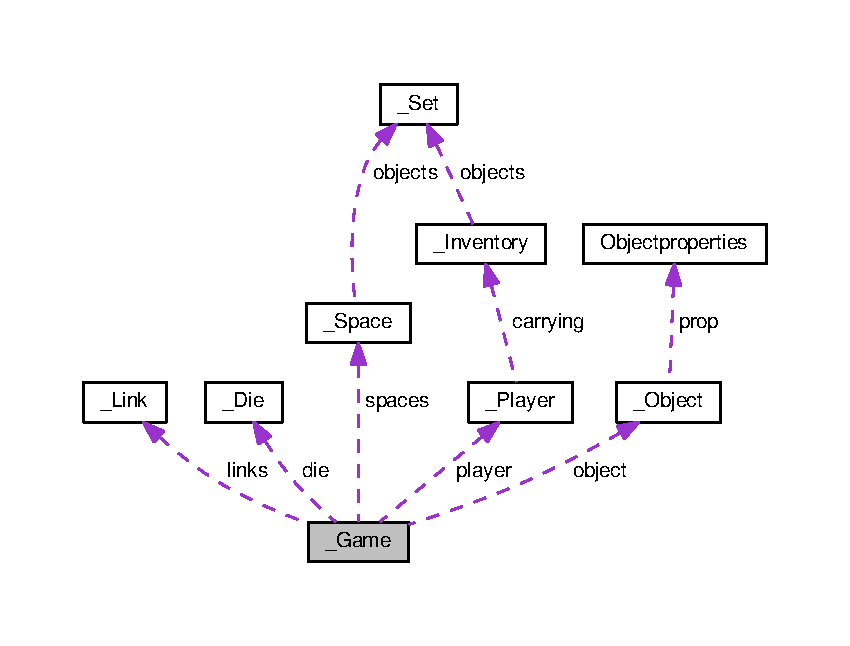
\includegraphics[width=350pt]{struct__Game__coll__graph}
\end{center}
\end{figure}
\subsection*{Data Fields}
\begin{DoxyCompactItemize}
\item 
\hyperlink{player_8h_af30e2030635a69690f85e48bc6ef202f}{Player} $\ast$ \hyperlink{struct__Game_a31406605782d71ec00c4bf258ea76267}{player}
\item 
\hyperlink{object_8h_a7f8bbcda919b65ce67f92fba08e0212f}{Object} $\ast$ \hyperlink{struct__Game_a805ef4ca82198bff524ed40d8ae867e7}{object} \mbox{[}\hyperlink{game_8h_a8e497c59a3362df6102c893a8498acd0}{M\+A\+X\+\_\+\+O\+BJ}\mbox{]}
\item 
\hyperlink{space_8h_a67533ffc2b70463baecc38fb0629bbfc}{Space} $\ast$ \hyperlink{struct__Game_ab4180417d9148f8abb2233ca6c4ecfe5}{spaces} \mbox{[}\hyperlink{space_8h_a5f54fd55f983a2e33ce076cd9f587e82}{M\+A\+X\+\_\+\+S\+P\+A\+C\+ES}+1\mbox{]}
\item 
\hyperlink{command_8h_a0473597db8c45c0289b6b8e2f8abbe32}{T\+\_\+\+Command} \hyperlink{struct__Game_a27727b50ea0904a1fe9e1c55c27f2cf1}{last\+\_\+cmd}
\item 
\hyperlink{die_8h_a892f0b0bf81d69a1f7a14ea238e36dd3}{Die} $\ast$ \hyperlink{struct__Game_a0d6009b5dcb080489c192a9198fa7d46}{die}
\item 
\hyperlink{types_8h_a32c27cc471df37f4fc818d65de0a56c4}{S\+T\+A\+T\+US} \hyperlink{struct__Game_ac553fd756c47abf8e7066c20f6b7dc82}{last\+\_\+command\+\_\+status}
\item 
char \hyperlink{struct__Game_a3aefc7ea654ec68acee732527bb660e8}{aux} \mbox{[}\hyperlink{types_8h_a92ed8507d1cd2331ad09275c5c4c1c89}{W\+O\+R\+D\+\_\+\+S\+I\+ZE}\mbox{]}
\item 
\hyperlink{link_8h_ae3b299941e67be6971bfd64a25505eff}{Link} $\ast$ \hyperlink{struct__Game_a2b766f0814f66dcf437600a9c526142e}{links} \mbox{[}\hyperlink{game_8h_a660ed1ec8604982002a0d6eced0e0367}{M\+A\+X\+\_\+\+L\+I\+N\+KS}\mbox{]}
\end{DoxyCompactItemize}


\subsection{Detailed Description}
game definition 

Struct for storing the elements of the game. 

\subsection{Field Documentation}
\index{\+\_\+\+Game@{\+\_\+\+Game}!aux@{aux}}
\index{aux@{aux}!\+\_\+\+Game@{\+\_\+\+Game}}
\subsubsection[{\texorpdfstring{aux}{aux}}]{\setlength{\rightskip}{0pt plus 5cm}char \+\_\+\+Game\+::aux\mbox{[}{\bf W\+O\+R\+D\+\_\+\+S\+I\+ZE}\mbox{]}}\hypertarget{struct__Game_a3aefc7ea654ec68acee732527bb660e8}{}\label{struct__Game_a3aefc7ea654ec68acee732527bb660e8}
character for writing \index{\+\_\+\+Game@{\+\_\+\+Game}!die@{die}}
\index{die@{die}!\+\_\+\+Game@{\+\_\+\+Game}}
\subsubsection[{\texorpdfstring{die}{die}}]{\setlength{\rightskip}{0pt plus 5cm}{\bf Die}$\ast$ \+\_\+\+Game\+::die}\hypertarget{struct__Game_a0d6009b5dcb080489c192a9198fa7d46}{}\label{struct__Game_a0d6009b5dcb080489c192a9198fa7d46}
Contains a die \index{\+\_\+\+Game@{\+\_\+\+Game}!last\+\_\+cmd@{last\+\_\+cmd}}
\index{last\+\_\+cmd@{last\+\_\+cmd}!\+\_\+\+Game@{\+\_\+\+Game}}
\subsubsection[{\texorpdfstring{last\+\_\+cmd}{last_cmd}}]{\setlength{\rightskip}{0pt plus 5cm}{\bf T\+\_\+\+Command} \+\_\+\+Game\+::last\+\_\+cmd}\hypertarget{struct__Game_a27727b50ea0904a1fe9e1c55c27f2cf1}{}\label{struct__Game_a27727b50ea0904a1fe9e1c55c27f2cf1}
Saves the last command typed \index{\+\_\+\+Game@{\+\_\+\+Game}!last\+\_\+command\+\_\+status@{last\+\_\+command\+\_\+status}}
\index{last\+\_\+command\+\_\+status@{last\+\_\+command\+\_\+status}!\+\_\+\+Game@{\+\_\+\+Game}}
\subsubsection[{\texorpdfstring{last\+\_\+command\+\_\+status}{last_command_status}}]{\setlength{\rightskip}{0pt plus 5cm}{\bf S\+T\+A\+T\+US} \+\_\+\+Game\+::last\+\_\+command\+\_\+status}\hypertarget{struct__Game_ac553fd756c47abf8e7066c20f6b7dc82}{}\label{struct__Game_ac553fd756c47abf8e7066c20f6b7dc82}
Saves the last command typed\textquotesingle{}s result \index{\+\_\+\+Game@{\+\_\+\+Game}!links@{links}}
\index{links@{links}!\+\_\+\+Game@{\+\_\+\+Game}}
\subsubsection[{\texorpdfstring{links}{links}}]{\setlength{\rightskip}{0pt plus 5cm}{\bf Link}$\ast$ \+\_\+\+Game\+::links\mbox{[}{\bf M\+A\+X\+\_\+\+L\+I\+N\+KS}\mbox{]}}\hypertarget{struct__Game_a2b766f0814f66dcf437600a9c526142e}{}\label{struct__Game_a2b766f0814f66dcf437600a9c526142e}
link variable \index{\+\_\+\+Game@{\+\_\+\+Game}!object@{object}}
\index{object@{object}!\+\_\+\+Game@{\+\_\+\+Game}}
\subsubsection[{\texorpdfstring{object}{object}}]{\setlength{\rightskip}{0pt plus 5cm}{\bf Object}$\ast$ \+\_\+\+Game\+::object\mbox{[}{\bf M\+A\+X\+\_\+\+O\+BJ}\mbox{]}}\hypertarget{struct__Game_a805ef4ca82198bff524ed40d8ae867e7}{}\label{struct__Game_a805ef4ca82198bff524ed40d8ae867e7}
Information about the object/s \index{\+\_\+\+Game@{\+\_\+\+Game}!player@{player}}
\index{player@{player}!\+\_\+\+Game@{\+\_\+\+Game}}
\subsubsection[{\texorpdfstring{player}{player}}]{\setlength{\rightskip}{0pt plus 5cm}{\bf Player}$\ast$ \+\_\+\+Game\+::player}\hypertarget{struct__Game_a31406605782d71ec00c4bf258ea76267}{}\label{struct__Game_a31406605782d71ec00c4bf258ea76267}
Information about the player/s \index{\+\_\+\+Game@{\+\_\+\+Game}!spaces@{spaces}}
\index{spaces@{spaces}!\+\_\+\+Game@{\+\_\+\+Game}}
\subsubsection[{\texorpdfstring{spaces}{spaces}}]{\setlength{\rightskip}{0pt plus 5cm}{\bf Space}$\ast$ \+\_\+\+Game\+::spaces\mbox{[}{\bf M\+A\+X\+\_\+\+S\+P\+A\+C\+ES}+1\mbox{]}}\hypertarget{struct__Game_ab4180417d9148f8abb2233ca6c4ecfe5}{}\label{struct__Game_ab4180417d9148f8abb2233ca6c4ecfe5}
Information about the spaces defined in the board 

The documentation for this struct was generated from the following file\+:\begin{DoxyCompactItemize}
\item 
src/\hyperlink{game_8c}{game.\+c}\end{DoxyCompactItemize}

\hypertarget{struct__Graphic__engine}{}\section{\+\_\+\+Graphic\+\_\+engine Struct Reference}
\label{struct__Graphic__engine}\index{\+\_\+\+Graphic\+\_\+engine@{\+\_\+\+Graphic\+\_\+engine}}


graphic design  




Collaboration diagram for \+\_\+\+Graphic\+\_\+engine\+:
\nopagebreak
\begin{figure}[H]
\begin{center}
\leavevmode
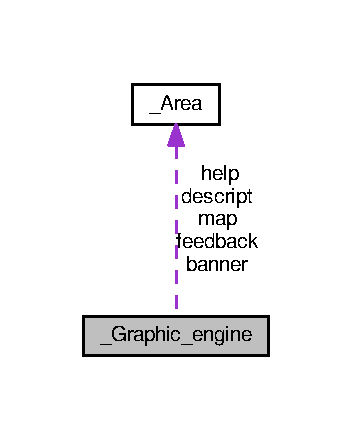
\includegraphics[width=169pt]{struct__Graphic__engine__coll__graph}
\end{center}
\end{figure}
\subsection*{Data Fields}
\begin{DoxyCompactItemize}
\item 
\hyperlink{screen_8h_acfdfc42f6522d75fa3c16713afde8127}{Area} $\ast$ \hyperlink{struct__Graphic__engine_a1ea06bb881d335da8c31d63b3e834bdb}{map}
\item 
\hyperlink{screen_8h_acfdfc42f6522d75fa3c16713afde8127}{Area} $\ast$ \hyperlink{struct__Graphic__engine_a414bb888ecce3389c7ce348264758e58}{descript}
\item 
\hyperlink{screen_8h_acfdfc42f6522d75fa3c16713afde8127}{Area} $\ast$ \hyperlink{struct__Graphic__engine_a440dfb2c23c3c4b7d3871187371117b9}{banner}
\item 
\hyperlink{screen_8h_acfdfc42f6522d75fa3c16713afde8127}{Area} $\ast$ \hyperlink{struct__Graphic__engine_ade1d3e95ad6def427f613a4a2d101875}{help}
\item 
\hyperlink{screen_8h_acfdfc42f6522d75fa3c16713afde8127}{Area} $\ast$ \hyperlink{struct__Graphic__engine_a4fc0ef353d000b20d57fb75d898c6d2d}{feedback}
\end{DoxyCompactItemize}


\subsection{Detailed Description}
graphic design 

Struct that include the variables that will help us show the design of our game. 

\subsection{Field Documentation}
\index{\+\_\+\+Graphic\+\_\+engine@{\+\_\+\+Graphic\+\_\+engine}!banner@{banner}}
\index{banner@{banner}!\+\_\+\+Graphic\+\_\+engine@{\+\_\+\+Graphic\+\_\+engine}}
\subsubsection[{\texorpdfstring{banner}{banner}}]{\setlength{\rightskip}{0pt plus 5cm}{\bf Area}$\ast$ \+\_\+\+Graphic\+\_\+engine\+::banner}\hypertarget{struct__Graphic__engine_a440dfb2c23c3c4b7d3871187371117b9}{}\label{struct__Graphic__engine_a440dfb2c23c3c4b7d3871187371117b9}
pointer to area (banner) \index{\+\_\+\+Graphic\+\_\+engine@{\+\_\+\+Graphic\+\_\+engine}!descript@{descript}}
\index{descript@{descript}!\+\_\+\+Graphic\+\_\+engine@{\+\_\+\+Graphic\+\_\+engine}}
\subsubsection[{\texorpdfstring{descript}{descript}}]{\setlength{\rightskip}{0pt plus 5cm}{\bf Area}$\ast$ \+\_\+\+Graphic\+\_\+engine\+::descript}\hypertarget{struct__Graphic__engine_a414bb888ecce3389c7ce348264758e58}{}\label{struct__Graphic__engine_a414bb888ecce3389c7ce348264758e58}
pointer to area (description) \index{\+\_\+\+Graphic\+\_\+engine@{\+\_\+\+Graphic\+\_\+engine}!feedback@{feedback}}
\index{feedback@{feedback}!\+\_\+\+Graphic\+\_\+engine@{\+\_\+\+Graphic\+\_\+engine}}
\subsubsection[{\texorpdfstring{feedback}{feedback}}]{\setlength{\rightskip}{0pt plus 5cm}{\bf Area}$\ast$ \+\_\+\+Graphic\+\_\+engine\+::feedback}\hypertarget{struct__Graphic__engine_a4fc0ef353d000b20d57fb75d898c6d2d}{}\label{struct__Graphic__engine_a4fc0ef353d000b20d57fb75d898c6d2d}
pointer to area (feedback) \index{\+\_\+\+Graphic\+\_\+engine@{\+\_\+\+Graphic\+\_\+engine}!help@{help}}
\index{help@{help}!\+\_\+\+Graphic\+\_\+engine@{\+\_\+\+Graphic\+\_\+engine}}
\subsubsection[{\texorpdfstring{help}{help}}]{\setlength{\rightskip}{0pt plus 5cm}{\bf Area}$\ast$ \+\_\+\+Graphic\+\_\+engine\+::help}\hypertarget{struct__Graphic__engine_ade1d3e95ad6def427f613a4a2d101875}{}\label{struct__Graphic__engine_ade1d3e95ad6def427f613a4a2d101875}
pointer to area (help) \index{\+\_\+\+Graphic\+\_\+engine@{\+\_\+\+Graphic\+\_\+engine}!map@{map}}
\index{map@{map}!\+\_\+\+Graphic\+\_\+engine@{\+\_\+\+Graphic\+\_\+engine}}
\subsubsection[{\texorpdfstring{map}{map}}]{\setlength{\rightskip}{0pt plus 5cm}{\bf Area}$\ast$ \+\_\+\+Graphic\+\_\+engine\+::map}\hypertarget{struct__Graphic__engine_a1ea06bb881d335da8c31d63b3e834bdb}{}\label{struct__Graphic__engine_a1ea06bb881d335da8c31d63b3e834bdb}
pointer to area (map) 

The documentation for this struct was generated from the following file\+:\begin{DoxyCompactItemize}
\item 
src/\hyperlink{graphic__engine_8c}{graphic\+\_\+engine.\+c}\end{DoxyCompactItemize}

\hypertarget{struct__Inventory}{}\section{\+\_\+\+Inventory Struct Reference}
\label{struct__Inventory}\index{\+\_\+\+Inventory@{\+\_\+\+Inventory}}


set and max objects.  




Collaboration diagram for \+\_\+\+Inventory\+:
\nopagebreak
\begin{figure}[H]
\begin{center}
\leavevmode
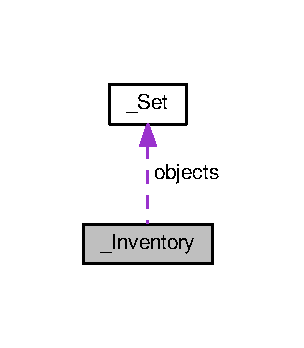
\includegraphics[width=146pt]{struct__Inventory__coll__graph}
\end{center}
\end{figure}
\subsection*{Data Fields}
\begin{DoxyCompactItemize}
\item 
\hyperlink{set_8h_a6d3b7f7c92cbb4577ef3ef7ddbf93161}{Set} $\ast$ \hyperlink{struct__Inventory_a478e4b50a62b9e7d5b17e335319faa97}{objects}
\item 
int \hyperlink{struct__Inventory_a230ffe8c2f84e67f284d43f8a8622d53}{num}
\end{DoxyCompactItemize}


\subsection{Detailed Description}
set and max objects. 

Struct for organising the objects using a pointer to set and a maximum number of objects(int). 

\subsection{Field Documentation}
\index{\+\_\+\+Inventory@{\+\_\+\+Inventory}!num@{num}}
\index{num@{num}!\+\_\+\+Inventory@{\+\_\+\+Inventory}}
\subsubsection[{\texorpdfstring{num}{num}}]{\setlength{\rightskip}{0pt plus 5cm}int \+\_\+\+Inventory\+::num}\hypertarget{struct__Inventory_a230ffe8c2f84e67f284d43f8a8622d53}{}\label{struct__Inventory_a230ffe8c2f84e67f284d43f8a8622d53}
max number of objects \index{\+\_\+\+Inventory@{\+\_\+\+Inventory}!objects@{objects}}
\index{objects@{objects}!\+\_\+\+Inventory@{\+\_\+\+Inventory}}
\subsubsection[{\texorpdfstring{objects}{objects}}]{\setlength{\rightskip}{0pt plus 5cm}{\bf Set}$\ast$ \+\_\+\+Inventory\+::objects}\hypertarget{struct__Inventory_a478e4b50a62b9e7d5b17e335319faa97}{}\label{struct__Inventory_a478e4b50a62b9e7d5b17e335319faa97}
set of ids 

The documentation for this struct was generated from the following file\+:\begin{DoxyCompactItemize}
\item 
src/inventory.\+c\end{DoxyCompactItemize}

\hypertarget{struct__Link}{}\section{\+\_\+\+Link Struct Reference}
\label{struct__Link}\index{\+\_\+\+Link@{\+\_\+\+Link}}


link definition  


\subsection*{Data Fields}
\begin{DoxyCompactItemize}
\item 
\hyperlink{types_8h_a845e604fb28f7e3d97549da3448149d3}{Id} \hyperlink{struct__Link_a151212e7a8e8274c2a1ee991ba95878b}{id}
\item 
char \hyperlink{struct__Link_a020ee863120055b29609157b9de3c84d}{name} \mbox{[}\hyperlink{types_8h_a92ed8507d1cd2331ad09275c5c4c1c89}{W\+O\+R\+D\+\_\+\+S\+I\+ZE}+1\mbox{]}
\item 
\hyperlink{types_8h_a845e604fb28f7e3d97549da3448149d3}{Id} \hyperlink{struct__Link_a5e7fbb3e1b15bf0cf981153c08be0729}{link1}
\item 
\hyperlink{types_8h_a845e604fb28f7e3d97549da3448149d3}{Id} \hyperlink{struct__Link_a7ea0ebc1c732428f2cc7e66b6b8832e4}{link2}
\item 
\hyperlink{types_8h_a3425906c2a1ce4f324e3b2006ece02cd}{L\+I\+N\+K\+\_\+\+ST} \hyperlink{struct__Link_a48f4cacf668ee2063e79d927bf50578a}{mode}
\item 
\hyperlink{types_8h_a845e604fb28f7e3d97549da3448149d3}{Id} \hyperlink{struct__Link_a51a17371bac3cb3d09e011a95da238b6}{key}
\end{DoxyCompactItemize}


\subsection{Detailed Description}
link definition 

Struct for storing a link with its properties. 

\subsection{Field Documentation}
\index{\+\_\+\+Link@{\+\_\+\+Link}!id@{id}}
\index{id@{id}!\+\_\+\+Link@{\+\_\+\+Link}}
\subsubsection[{\texorpdfstring{id}{id}}]{\setlength{\rightskip}{0pt plus 5cm}{\bf Id} \+\_\+\+Link\+::id}\hypertarget{struct__Link_a151212e7a8e8274c2a1ee991ba95878b}{}\label{struct__Link_a151212e7a8e8274c2a1ee991ba95878b}
id (long int) \index{\+\_\+\+Link@{\+\_\+\+Link}!key@{key}}
\index{key@{key}!\+\_\+\+Link@{\+\_\+\+Link}}
\subsubsection[{\texorpdfstring{key}{key}}]{\setlength{\rightskip}{0pt plus 5cm}{\bf Id} \+\_\+\+Link\+::key}\hypertarget{struct__Link_a51a17371bac3cb3d09e011a95da238b6}{}\label{struct__Link_a51a17371bac3cb3d09e011a95da238b6}
key id \index{\+\_\+\+Link@{\+\_\+\+Link}!link1@{link1}}
\index{link1@{link1}!\+\_\+\+Link@{\+\_\+\+Link}}
\subsubsection[{\texorpdfstring{link1}{link1}}]{\setlength{\rightskip}{0pt plus 5cm}{\bf Id} \+\_\+\+Link\+::link1}\hypertarget{struct__Link_a5e7fbb3e1b15bf0cf981153c08be0729}{}\label{struct__Link_a5e7fbb3e1b15bf0cf981153c08be0729}
L\+E\+FT L\+I\+NK (north/west) \index{\+\_\+\+Link@{\+\_\+\+Link}!link2@{link2}}
\index{link2@{link2}!\+\_\+\+Link@{\+\_\+\+Link}}
\subsubsection[{\texorpdfstring{link2}{link2}}]{\setlength{\rightskip}{0pt plus 5cm}{\bf Id} \+\_\+\+Link\+::link2}\hypertarget{struct__Link_a7ea0ebc1c732428f2cc7e66b6b8832e4}{}\label{struct__Link_a7ea0ebc1c732428f2cc7e66b6b8832e4}
R\+I\+G\+HT L\+I\+NK (south/east) \index{\+\_\+\+Link@{\+\_\+\+Link}!mode@{mode}}
\index{mode@{mode}!\+\_\+\+Link@{\+\_\+\+Link}}
\subsubsection[{\texorpdfstring{mode}{mode}}]{\setlength{\rightskip}{0pt plus 5cm}{\bf L\+I\+N\+K\+\_\+\+ST} \+\_\+\+Link\+::mode}\hypertarget{struct__Link_a48f4cacf668ee2063e79d927bf50578a}{}\label{struct__Link_a48f4cacf668ee2063e79d927bf50578a}
link enumeration \index{\+\_\+\+Link@{\+\_\+\+Link}!name@{name}}
\index{name@{name}!\+\_\+\+Link@{\+\_\+\+Link}}
\subsubsection[{\texorpdfstring{name}{name}}]{\setlength{\rightskip}{0pt plus 5cm}char \+\_\+\+Link\+::name\mbox{[}{\bf W\+O\+R\+D\+\_\+\+S\+I\+ZE}+1\mbox{]}}\hypertarget{struct__Link_a020ee863120055b29609157b9de3c84d}{}\label{struct__Link_a020ee863120055b29609157b9de3c84d}
char string 

The documentation for this struct was generated from the following file\+:\begin{DoxyCompactItemize}
\item 
src/link.\+c\end{DoxyCompactItemize}

\hypertarget{struct__Object}{}\section{\+\_\+\+Object Struct Reference}
\label{struct__Object}\index{\+\_\+\+Object@{\+\_\+\+Object}}


object of the game  




Collaboration diagram for \+\_\+\+Object\+:
\nopagebreak
\begin{figure}[H]
\begin{center}
\leavevmode
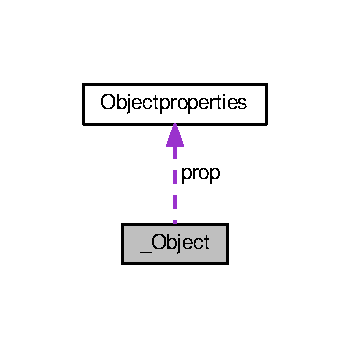
\includegraphics[width=168pt]{struct__Object__coll__graph}
\end{center}
\end{figure}
\subsection*{Data Fields}
\begin{DoxyCompactItemize}
\item 
\hyperlink{types_8h_a845e604fb28f7e3d97549da3448149d3}{Id} \hyperlink{struct__Object_a3cff7a0e8dc4e9d23895ed9af1b7653a}{id}
\item 
\hyperlink{types_8h_a845e604fb28f7e3d97549da3448149d3}{Id} \hyperlink{struct__Object_a3c596b8898734de2f71fd1a33dfa72fb}{location}
\item 
\hyperlink{types_8h_a845e604fb28f7e3d97549da3448149d3}{Id} \hyperlink{struct__Object_a14c4dfa849520565b86f235c87827546}{initialpos}
\item 
char \hyperlink{struct__Object_ada77f97bbe2b9be36715adba222eebc6}{name} \mbox{[}\hyperlink{object_8h_a88b1ded1b83576bfb0683aeab25ae052}{M\+A\+X\+O\+B\+J\+N\+A\+ME}\mbox{]}
\item 
char \hyperlink{struct__Object_ae9fbe2f03c6902aa879c5ff437fa2444}{sdescription} \mbox{[}\hyperlink{types_8h_a2b9d4cb1200ff8c085b0a4902e0d7229}{M\+A\+X\+\_\+\+D\+E\+S\+C\+R\+I\+P\+T\+I\+ON}\mbox{]}
\item 
char \hyperlink{struct__Object_ace9493f4f8d73f26e2cc79bb65bf6309}{ldescription} \mbox{[}\hyperlink{types_8h_a2b9d4cb1200ff8c085b0a4902e0d7229}{M\+A\+X\+\_\+\+D\+E\+S\+C\+R\+I\+P\+T\+I\+ON}\mbox{]}
\item 
\hyperlink{structObjectproperties}{Objectproperties} \hyperlink{struct__Object_a2acdcc90e7417c2ab1bc41e52a107c2d}{prop}
\end{DoxyCompactItemize}


\subsection{Detailed Description}
object of the game 

Struct for storing the different variables that an object should have 

\subsection{Field Documentation}
\index{\+\_\+\+Object@{\+\_\+\+Object}!id@{id}}
\index{id@{id}!\+\_\+\+Object@{\+\_\+\+Object}}
\subsubsection[{\texorpdfstring{id}{id}}]{\setlength{\rightskip}{0pt plus 5cm}{\bf Id} \+\_\+\+Object\+::id}\hypertarget{struct__Object_a3cff7a0e8dc4e9d23895ed9af1b7653a}{}\label{struct__Object_a3cff7a0e8dc4e9d23895ed9af1b7653a}
Object identifier \index{\+\_\+\+Object@{\+\_\+\+Object}!initialpos@{initialpos}}
\index{initialpos@{initialpos}!\+\_\+\+Object@{\+\_\+\+Object}}
\subsubsection[{\texorpdfstring{initialpos}{initialpos}}]{\setlength{\rightskip}{0pt plus 5cm}{\bf Id} \+\_\+\+Object\+::initialpos}\hypertarget{struct__Object_a14c4dfa849520565b86f235c87827546}{}\label{struct__Object_a14c4dfa849520565b86f235c87827546}
Original object location \index{\+\_\+\+Object@{\+\_\+\+Object}!ldescription@{ldescription}}
\index{ldescription@{ldescription}!\+\_\+\+Object@{\+\_\+\+Object}}
\subsubsection[{\texorpdfstring{ldescription}{ldescription}}]{\setlength{\rightskip}{0pt plus 5cm}char \+\_\+\+Object\+::ldescription\mbox{[}{\bf M\+A\+X\+\_\+\+D\+E\+S\+C\+R\+I\+P\+T\+I\+ON}\mbox{]}}\hypertarget{struct__Object_ace9493f4f8d73f26e2cc79bb65bf6309}{}\label{struct__Object_ace9493f4f8d73f26e2cc79bb65bf6309}
Object description to be shown ingame (moved) \index{\+\_\+\+Object@{\+\_\+\+Object}!location@{location}}
\index{location@{location}!\+\_\+\+Object@{\+\_\+\+Object}}
\subsubsection[{\texorpdfstring{location}{location}}]{\setlength{\rightskip}{0pt plus 5cm}{\bf Id} \+\_\+\+Object\+::location}\hypertarget{struct__Object_a3c596b8898734de2f71fd1a33dfa72fb}{}\label{struct__Object_a3c596b8898734de2f71fd1a33dfa72fb}
Object location \index{\+\_\+\+Object@{\+\_\+\+Object}!name@{name}}
\index{name@{name}!\+\_\+\+Object@{\+\_\+\+Object}}
\subsubsection[{\texorpdfstring{name}{name}}]{\setlength{\rightskip}{0pt plus 5cm}char \+\_\+\+Object\+::name\mbox{[}{\bf M\+A\+X\+O\+B\+J\+N\+A\+ME}\mbox{]}}\hypertarget{struct__Object_ada77f97bbe2b9be36715adba222eebc6}{}\label{struct__Object_ada77f97bbe2b9be36715adba222eebc6}
Object name to be shown ingame \index{\+\_\+\+Object@{\+\_\+\+Object}!prop@{prop}}
\index{prop@{prop}!\+\_\+\+Object@{\+\_\+\+Object}}
\subsubsection[{\texorpdfstring{prop}{prop}}]{\setlength{\rightskip}{0pt plus 5cm}{\bf Objectproperties} \+\_\+\+Object\+::prop}\hypertarget{struct__Object_a2acdcc90e7417c2ab1bc41e52a107c2d}{}\label{struct__Object_a2acdcc90e7417c2ab1bc41e52a107c2d}
Struct properties \index{\+\_\+\+Object@{\+\_\+\+Object}!sdescription@{sdescription}}
\index{sdescription@{sdescription}!\+\_\+\+Object@{\+\_\+\+Object}}
\subsubsection[{\texorpdfstring{sdescription}{sdescription}}]{\setlength{\rightskip}{0pt plus 5cm}char \+\_\+\+Object\+::sdescription\mbox{[}{\bf M\+A\+X\+\_\+\+D\+E\+S\+C\+R\+I\+P\+T\+I\+ON}\mbox{]}}\hypertarget{struct__Object_ae9fbe2f03c6902aa879c5ff437fa2444}{}\label{struct__Object_ae9fbe2f03c6902aa879c5ff437fa2444}
Object description to be shown ingame (original) 

The documentation for this struct was generated from the following file\+:\begin{DoxyCompactItemize}
\item 
src/\hyperlink{object_8c}{object.\+c}\end{DoxyCompactItemize}

\hypertarget{struct__Player}{}\section{\+\_\+\+Player Struct Reference}
\label{struct__Player}\index{\+\_\+\+Player@{\+\_\+\+Player}}


player definition  




Collaboration diagram for \+\_\+\+Player\+:
\nopagebreak
\begin{figure}[H]
\begin{center}
\leavevmode
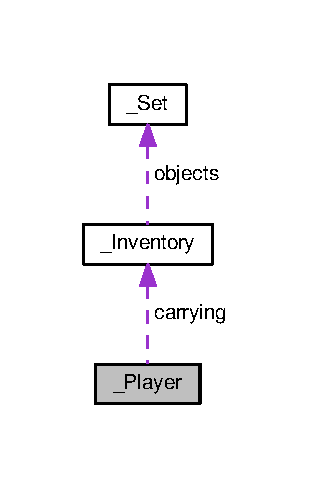
\includegraphics[width=149pt]{struct__Player__coll__graph}
\end{center}
\end{figure}
\subsection*{Data Fields}
\begin{DoxyCompactItemize}
\item 
\hyperlink{types_8h_a845e604fb28f7e3d97549da3448149d3}{Id} \hyperlink{struct__Player_a60d635cd063816a9c1bd873f4868bb90}{id}
\item 
char \hyperlink{struct__Player_ae3931f4219966e5a8b9fd2621f26956a}{name} \mbox{[}\hyperlink{player_8h_a5bb4369b60f4886b73026bb884053640}{M\+A\+X\+P\+L\+A\+Y\+N\+A\+ME}\mbox{]}
\item 
\hyperlink{types_8h_a845e604fb28f7e3d97549da3448149d3}{Id} \hyperlink{struct__Player_adbb6195d15b88f3f658e74274eff52d8}{location}
\item 
\hyperlink{inventory_8h_a2253bf64ac4ce6a9c1d6f39c0b0d32a3}{Inventory} $\ast$ \hyperlink{struct__Player_a816df014a3e27f7ef65b16007bc26b41}{carrying}
\end{DoxyCompactItemize}


\subsection{Detailed Description}
player definition 

The Player structure contains the player related information Privacy\+: private structure Struct for storing a player and the elements it will use while playing. 

\subsection{Field Documentation}
\index{\+\_\+\+Player@{\+\_\+\+Player}!carrying@{carrying}}
\index{carrying@{carrying}!\+\_\+\+Player@{\+\_\+\+Player}}
\subsubsection[{\texorpdfstring{carrying}{carrying}}]{\setlength{\rightskip}{0pt plus 5cm}{\bf Inventory}$\ast$ \+\_\+\+Player\+::carrying}\hypertarget{struct__Player_a816df014a3e27f7ef65b16007bc26b41}{}\label{struct__Player_a816df014a3e27f7ef65b16007bc26b41}
objects that player will carry \index{\+\_\+\+Player@{\+\_\+\+Player}!id@{id}}
\index{id@{id}!\+\_\+\+Player@{\+\_\+\+Player}}
\subsubsection[{\texorpdfstring{id}{id}}]{\setlength{\rightskip}{0pt plus 5cm}{\bf Id} \+\_\+\+Player\+::id}\hypertarget{struct__Player_a60d635cd063816a9c1bd873f4868bb90}{}\label{struct__Player_a60d635cd063816a9c1bd873f4868bb90}
Player Identifier ingame \index{\+\_\+\+Player@{\+\_\+\+Player}!location@{location}}
\index{location@{location}!\+\_\+\+Player@{\+\_\+\+Player}}
\subsubsection[{\texorpdfstring{location}{location}}]{\setlength{\rightskip}{0pt plus 5cm}{\bf Id} \+\_\+\+Player\+::location}\hypertarget{struct__Player_adbb6195d15b88f3f658e74274eff52d8}{}\label{struct__Player_adbb6195d15b88f3f658e74274eff52d8}
Additional ID, for saving the space where the player is located \index{\+\_\+\+Player@{\+\_\+\+Player}!name@{name}}
\index{name@{name}!\+\_\+\+Player@{\+\_\+\+Player}}
\subsubsection[{\texorpdfstring{name}{name}}]{\setlength{\rightskip}{0pt plus 5cm}char \+\_\+\+Player\+::name\mbox{[}{\bf M\+A\+X\+P\+L\+A\+Y\+N\+A\+ME}\mbox{]}}\hypertarget{struct__Player_ae3931f4219966e5a8b9fd2621f26956a}{}\label{struct__Player_ae3931f4219966e5a8b9fd2621f26956a}
Player name 

The documentation for this struct was generated from the following file\+:\begin{DoxyCompactItemize}
\item 
src/\hyperlink{player_8c}{player.\+c}\end{DoxyCompactItemize}

\hypertarget{struct__Set}{}\section{\+\_\+\+Set Struct Reference}
\label{struct__Set}\index{\+\_\+\+Set@{\+\_\+\+Set}}


id and number of ids  


\subsection*{Data Fields}
\begin{DoxyCompactItemize}
\item 
\hyperlink{types_8h_a845e604fb28f7e3d97549da3448149d3}{Id} \hyperlink{struct__Set_a1b17ea0ae355f78db02768ad4e6fd85d}{ids} \mbox{[}M\+A\+X\+S\+ET\mbox{]}
\item 
int \hyperlink{struct__Set_a9bdd7b9ab8cf4d6568c4eea567f8e56a}{nids}
\end{DoxyCompactItemize}


\subsection{Detailed Description}
id and number of ids 

Struct for managing the values and adding ids by using an id and the number of ids. 

\subsection{Field Documentation}
\index{\+\_\+\+Set@{\+\_\+\+Set}!ids@{ids}}
\index{ids@{ids}!\+\_\+\+Set@{\+\_\+\+Set}}
\subsubsection[{\texorpdfstring{ids}{ids}}]{\setlength{\rightskip}{0pt plus 5cm}{\bf Id} \+\_\+\+Set\+::ids\mbox{[}M\+A\+X\+S\+ET\mbox{]}}\hypertarget{struct__Set_a1b17ea0ae355f78db02768ad4e6fd85d}{}\label{struct__Set_a1b17ea0ae355f78db02768ad4e6fd85d}
id (long int) \index{\+\_\+\+Set@{\+\_\+\+Set}!nids@{nids}}
\index{nids@{nids}!\+\_\+\+Set@{\+\_\+\+Set}}
\subsubsection[{\texorpdfstring{nids}{nids}}]{\setlength{\rightskip}{0pt plus 5cm}int \+\_\+\+Set\+::nids}\hypertarget{struct__Set_a9bdd7b9ab8cf4d6568c4eea567f8e56a}{}\label{struct__Set_a9bdd7b9ab8cf4d6568c4eea567f8e56a}
number of ids 

The documentation for this struct was generated from the following file\+:\begin{DoxyCompactItemize}
\item 
src/set.\+c\end{DoxyCompactItemize}

\hypertarget{struct__Space}{}\section{\+\_\+\+Space Struct Reference}
\label{struct__Space}\index{\+\_\+\+Space@{\+\_\+\+Space}}


spaces of the game  




Collaboration diagram for \+\_\+\+Space\+:
\nopagebreak
\begin{figure}[H]
\begin{center}
\leavevmode
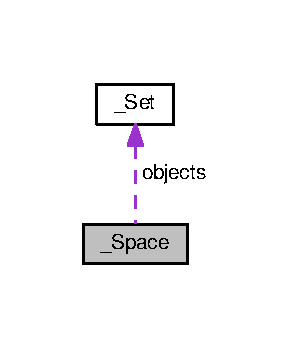
\includegraphics[width=140pt]{struct__Space__coll__graph}
\end{center}
\end{figure}
\subsection*{Data Fields}
\begin{DoxyCompactItemize}
\item 
\hyperlink{types_8h_a845e604fb28f7e3d97549da3448149d3}{Id} \hyperlink{struct__Space_a70cb461deb9ac073e401b607339b567f}{id}
\item 
char \hyperlink{struct__Space_aa1c9c994c2d16ecf3ef46138685fdfdc}{name} \mbox{[}\hyperlink{types_8h_a92ed8507d1cd2331ad09275c5c4c1c89}{W\+O\+R\+D\+\_\+\+S\+I\+ZE}+1\mbox{]}
\item 
\hyperlink{types_8h_a845e604fb28f7e3d97549da3448149d3}{Id} \hyperlink{struct__Space_ae5ebe53ce79514d7d2d93911e0159252}{north}
\item 
\hyperlink{types_8h_a845e604fb28f7e3d97549da3448149d3}{Id} \hyperlink{struct__Space_a646b68c22a0bbf1685033c96109d31d1}{south}
\item 
\hyperlink{types_8h_a845e604fb28f7e3d97549da3448149d3}{Id} \hyperlink{struct__Space_a41ce2bf33cf0c157b358221f094ee05b}{east}
\item 
\hyperlink{types_8h_a845e604fb28f7e3d97549da3448149d3}{Id} \hyperlink{struct__Space_a20c1d259e93b44e24ba82982e142eb9b}{west}
\item 
\hyperlink{types_8h_a845e604fb28f7e3d97549da3448149d3}{Id} \hyperlink{struct__Space_af2a50145d93dfb8d82b8b42138dc57a1}{up}
\item 
\hyperlink{types_8h_a845e604fb28f7e3d97549da3448149d3}{Id} \hyperlink{struct__Space_ac20194f418676bb03cca7e0fdcb6f559}{down}
\item 
\hyperlink{set_8h_a6d3b7f7c92cbb4577ef3ef7ddbf93161}{Set} $\ast$ \hyperlink{struct__Space_a661ed8b0fc8085b6db70188aa5085625}{objects}
\item 
char \hyperlink{struct__Space_a60637342523b393b7cae073324f57be2}{gdesc} \mbox{[}30\mbox{]}\mbox{[}110\mbox{]}
\item 
char \hyperlink{struct__Space_af8b371dd53e49a83a287175f0e686245}{sdescription} \mbox{[}\hyperlink{types_8h_a2b9d4cb1200ff8c085b0a4902e0d7229}{M\+A\+X\+\_\+\+D\+E\+S\+C\+R\+I\+P\+T\+I\+ON}\mbox{]}
\item 
char \hyperlink{struct__Space_a6cf737a07c4a3cd79aa80062a06d73d3}{ldescription} \mbox{[}\hyperlink{types_8h_a3a96a0e39038d30582bfa0cf12e87f0c}{M\+A\+X\+\_\+\+L\+O\+N\+G\+\_\+\+D\+E\+S\+C\+R\+I\+P\+T\+I\+ON}\mbox{]}
\item 
\hyperlink{types_8h_a3e5b8192e7d9ffaf3542f1210aec18dd}{B\+O\+OL} \hyperlink{struct__Space_a3e7f0cd158600936103895aa2bb9f0b4}{iluminate}
\end{DoxyCompactItemize}


\subsection{Detailed Description}
spaces of the game 

The space structure codes the maps (saved in data.\+dat) Privacy\+: private structure Struct for storing the different variables and characteristics that spaces should have. 

\subsection{Field Documentation}
\index{\+\_\+\+Space@{\+\_\+\+Space}!down@{down}}
\index{down@{down}!\+\_\+\+Space@{\+\_\+\+Space}}
\subsubsection[{\texorpdfstring{down}{down}}]{\setlength{\rightskip}{0pt plus 5cm}{\bf Id} \+\_\+\+Space\+::down}\hypertarget{struct__Space_ac20194f418676bb03cca7e0fdcb6f559}{}\label{struct__Space_ac20194f418676bb03cca7e0fdcb6f559}
Id of the space located downwards \index{\+\_\+\+Space@{\+\_\+\+Space}!east@{east}}
\index{east@{east}!\+\_\+\+Space@{\+\_\+\+Space}}
\subsubsection[{\texorpdfstring{east}{east}}]{\setlength{\rightskip}{0pt plus 5cm}{\bf Id} \+\_\+\+Space\+::east}\hypertarget{struct__Space_a41ce2bf33cf0c157b358221f094ee05b}{}\label{struct__Space_a41ce2bf33cf0c157b358221f094ee05b}
Id of the space located in the east \index{\+\_\+\+Space@{\+\_\+\+Space}!gdesc@{gdesc}}
\index{gdesc@{gdesc}!\+\_\+\+Space@{\+\_\+\+Space}}
\subsubsection[{\texorpdfstring{gdesc}{gdesc}}]{\setlength{\rightskip}{0pt plus 5cm}char \+\_\+\+Space\+::gdesc\mbox{[}30\mbox{]}\mbox{[}110\mbox{]}}\hypertarget{struct__Space_a60637342523b393b7cae073324f57be2}{}\label{struct__Space_a60637342523b393b7cae073324f57be2}
Graphic description \index{\+\_\+\+Space@{\+\_\+\+Space}!id@{id}}
\index{id@{id}!\+\_\+\+Space@{\+\_\+\+Space}}
\subsubsection[{\texorpdfstring{id}{id}}]{\setlength{\rightskip}{0pt plus 5cm}{\bf Id} \+\_\+\+Space\+::id}\hypertarget{struct__Space_a70cb461deb9ac073e401b607339b567f}{}\label{struct__Space_a70cb461deb9ac073e401b607339b567f}
Space identifier \index{\+\_\+\+Space@{\+\_\+\+Space}!iluminate@{iluminate}}
\index{iluminate@{iluminate}!\+\_\+\+Space@{\+\_\+\+Space}}
\subsubsection[{\texorpdfstring{iluminate}{iluminate}}]{\setlength{\rightskip}{0pt plus 5cm}{\bf B\+O\+OL} \+\_\+\+Space\+::iluminate}\hypertarget{struct__Space_a3e7f0cd158600936103895aa2bb9f0b4}{}\label{struct__Space_a3e7f0cd158600936103895aa2bb9f0b4}
space ilumination properties \index{\+\_\+\+Space@{\+\_\+\+Space}!ldescription@{ldescription}}
\index{ldescription@{ldescription}!\+\_\+\+Space@{\+\_\+\+Space}}
\subsubsection[{\texorpdfstring{ldescription}{ldescription}}]{\setlength{\rightskip}{0pt plus 5cm}char \+\_\+\+Space\+::ldescription\mbox{[}{\bf M\+A\+X\+\_\+\+L\+O\+N\+G\+\_\+\+D\+E\+S\+C\+R\+I\+P\+T\+I\+ON}\mbox{]}}\hypertarget{struct__Space_a6cf737a07c4a3cd79aa80062a06d73d3}{}\label{struct__Space_a6cf737a07c4a3cd79aa80062a06d73d3}
space description \index{\+\_\+\+Space@{\+\_\+\+Space}!name@{name}}
\index{name@{name}!\+\_\+\+Space@{\+\_\+\+Space}}
\subsubsection[{\texorpdfstring{name}{name}}]{\setlength{\rightskip}{0pt plus 5cm}char \+\_\+\+Space\+::name\mbox{[}{\bf W\+O\+R\+D\+\_\+\+S\+I\+ZE}+1\mbox{]}}\hypertarget{struct__Space_aa1c9c994c2d16ecf3ef46138685fdfdc}{}\label{struct__Space_aa1c9c994c2d16ecf3ef46138685fdfdc}
Space name \index{\+\_\+\+Space@{\+\_\+\+Space}!north@{north}}
\index{north@{north}!\+\_\+\+Space@{\+\_\+\+Space}}
\subsubsection[{\texorpdfstring{north}{north}}]{\setlength{\rightskip}{0pt plus 5cm}{\bf Id} \+\_\+\+Space\+::north}\hypertarget{struct__Space_ae5ebe53ce79514d7d2d93911e0159252}{}\label{struct__Space_ae5ebe53ce79514d7d2d93911e0159252}
Id of the space located in the north \index{\+\_\+\+Space@{\+\_\+\+Space}!objects@{objects}}
\index{objects@{objects}!\+\_\+\+Space@{\+\_\+\+Space}}
\subsubsection[{\texorpdfstring{objects}{objects}}]{\setlength{\rightskip}{0pt plus 5cm}{\bf Set}$\ast$ \+\_\+\+Space\+::objects}\hypertarget{struct__Space_a661ed8b0fc8085b6db70188aa5085625}{}\label{struct__Space_a661ed8b0fc8085b6db70188aa5085625}
Object located in that space \index{\+\_\+\+Space@{\+\_\+\+Space}!sdescription@{sdescription}}
\index{sdescription@{sdescription}!\+\_\+\+Space@{\+\_\+\+Space}}
\subsubsection[{\texorpdfstring{sdescription}{sdescription}}]{\setlength{\rightskip}{0pt plus 5cm}char \+\_\+\+Space\+::sdescription\mbox{[}{\bf M\+A\+X\+\_\+\+D\+E\+S\+C\+R\+I\+P\+T\+I\+ON}\mbox{]}}\hypertarget{struct__Space_af8b371dd53e49a83a287175f0e686245}{}\label{struct__Space_af8b371dd53e49a83a287175f0e686245}
space description \index{\+\_\+\+Space@{\+\_\+\+Space}!south@{south}}
\index{south@{south}!\+\_\+\+Space@{\+\_\+\+Space}}
\subsubsection[{\texorpdfstring{south}{south}}]{\setlength{\rightskip}{0pt plus 5cm}{\bf Id} \+\_\+\+Space\+::south}\hypertarget{struct__Space_a646b68c22a0bbf1685033c96109d31d1}{}\label{struct__Space_a646b68c22a0bbf1685033c96109d31d1}
Id of the space located in the south \index{\+\_\+\+Space@{\+\_\+\+Space}!up@{up}}
\index{up@{up}!\+\_\+\+Space@{\+\_\+\+Space}}
\subsubsection[{\texorpdfstring{up}{up}}]{\setlength{\rightskip}{0pt plus 5cm}{\bf Id} \+\_\+\+Space\+::up}\hypertarget{struct__Space_af2a50145d93dfb8d82b8b42138dc57a1}{}\label{struct__Space_af2a50145d93dfb8d82b8b42138dc57a1}
Id of the space located upwards \index{\+\_\+\+Space@{\+\_\+\+Space}!west@{west}}
\index{west@{west}!\+\_\+\+Space@{\+\_\+\+Space}}
\subsubsection[{\texorpdfstring{west}{west}}]{\setlength{\rightskip}{0pt plus 5cm}{\bf Id} \+\_\+\+Space\+::west}\hypertarget{struct__Space_a20c1d259e93b44e24ba82982e142eb9b}{}\label{struct__Space_a20c1d259e93b44e24ba82982e142eb9b}
Id of the space located in the west 

The documentation for this struct was generated from the following file\+:\begin{DoxyCompactItemize}
\item 
src/\hyperlink{space_8c}{space.\+c}\end{DoxyCompactItemize}

\hypertarget{structObjectproperties}{}\section{Objectproperties Struct Reference}
\label{structObjectproperties}\index{Objectproperties@{Objectproperties}}


properties of the objects in the game  


\subsection*{Data Fields}
\begin{DoxyCompactItemize}
\item 
\hyperlink{types_8h_a3e5b8192e7d9ffaf3542f1210aec18dd}{B\+O\+OL} \hyperlink{structObjectproperties_a565388c789e2f3333f0de535e19ac0fd}{Movable}
\item 
\hyperlink{types_8h_a3e5b8192e7d9ffaf3542f1210aec18dd}{B\+O\+OL} \hyperlink{structObjectproperties_a95af66b2771daa4b3509b28fb6ce904f}{Moved}
\item 
\hyperlink{types_8h_a3e5b8192e7d9ffaf3542f1210aec18dd}{B\+O\+OL} \hyperlink{structObjectproperties_ac7b53b9dc45c682287bf8a81ac29f5ea}{Hidden}
\item 
\hyperlink{types_8h_a845e604fb28f7e3d97549da3448149d3}{Id} \hyperlink{structObjectproperties_a346e3a6d314b69a30c356800c31ca3a0}{Open}
\item 
\hyperlink{types_8h_a3e5b8192e7d9ffaf3542f1210aec18dd}{B\+O\+OL} \hyperlink{structObjectproperties_ab32cc1dcd3dcb84df653c09d0560fe84}{Illuminate}
\item 
\hyperlink{types_8h_a3e5b8192e7d9ffaf3542f1210aec18dd}{B\+O\+OL} \hyperlink{structObjectproperties_a53e5cff11358955ab939ac4066aee6ff}{Switched\+On}
\end{DoxyCompactItemize}


\subsection{Detailed Description}
properties of the objects in the game 

The object structure places together the object id and name Privacy\+: private structure Struct for storing the different properties that an object should have 

\subsection{Field Documentation}
\index{Objectproperties@{Objectproperties}!Hidden@{Hidden}}
\index{Hidden@{Hidden}!Objectproperties@{Objectproperties}}
\subsubsection[{\texorpdfstring{Hidden}{Hidden}}]{\setlength{\rightskip}{0pt plus 5cm}{\bf B\+O\+OL} Objectproperties\+::\+Hidden}\hypertarget{structObjectproperties_ac7b53b9dc45c682287bf8a81ac29f5ea}{}\label{structObjectproperties_ac7b53b9dc45c682287bf8a81ac29f5ea}
Hidden property \index{Objectproperties@{Objectproperties}!Illuminate@{Illuminate}}
\index{Illuminate@{Illuminate}!Objectproperties@{Objectproperties}}
\subsubsection[{\texorpdfstring{Illuminate}{Illuminate}}]{\setlength{\rightskip}{0pt plus 5cm}{\bf B\+O\+OL} Objectproperties\+::\+Illuminate}\hypertarget{structObjectproperties_ab32cc1dcd3dcb84df653c09d0560fe84}{}\label{structObjectproperties_ab32cc1dcd3dcb84df653c09d0560fe84}
Iluminate property \index{Objectproperties@{Objectproperties}!Movable@{Movable}}
\index{Movable@{Movable}!Objectproperties@{Objectproperties}}
\subsubsection[{\texorpdfstring{Movable}{Movable}}]{\setlength{\rightskip}{0pt plus 5cm}{\bf B\+O\+OL} Objectproperties\+::\+Movable}\hypertarget{structObjectproperties_a565388c789e2f3333f0de535e19ac0fd}{}\label{structObjectproperties_a565388c789e2f3333f0de535e19ac0fd}
Movable property \index{Objectproperties@{Objectproperties}!Moved@{Moved}}
\index{Moved@{Moved}!Objectproperties@{Objectproperties}}
\subsubsection[{\texorpdfstring{Moved}{Moved}}]{\setlength{\rightskip}{0pt plus 5cm}{\bf B\+O\+OL} Objectproperties\+::\+Moved}\hypertarget{structObjectproperties_a95af66b2771daa4b3509b28fb6ce904f}{}\label{structObjectproperties_a95af66b2771daa4b3509b28fb6ce904f}
Moved property \index{Objectproperties@{Objectproperties}!Open@{Open}}
\index{Open@{Open}!Objectproperties@{Objectproperties}}
\subsubsection[{\texorpdfstring{Open}{Open}}]{\setlength{\rightskip}{0pt plus 5cm}{\bf Id} Objectproperties\+::\+Open}\hypertarget{structObjectproperties_a346e3a6d314b69a30c356800c31ca3a0}{}\label{structObjectproperties_a346e3a6d314b69a30c356800c31ca3a0}
Id status \index{Objectproperties@{Objectproperties}!Switched\+On@{Switched\+On}}
\index{Switched\+On@{Switched\+On}!Objectproperties@{Objectproperties}}
\subsubsection[{\texorpdfstring{Switched\+On}{SwitchedOn}}]{\setlength{\rightskip}{0pt plus 5cm}{\bf B\+O\+OL} Objectproperties\+::\+Switched\+On}\hypertarget{structObjectproperties_a53e5cff11358955ab939ac4066aee6ff}{}\label{structObjectproperties_a53e5cff11358955ab939ac4066aee6ff}
Switched\+On property 

The documentation for this struct was generated from the following file\+:\begin{DoxyCompactItemize}
\item 
src/\hyperlink{object_8c}{object.\+c}\end{DoxyCompactItemize}

\chapter{File Documentation}
\hypertarget{command_8h}{}\section{include/command.h File Reference}
\label{command_8h}\index{include/command.\+h@{include/command.\+h}}


Contains the command list and the declaration of the get user input function.  


This graph shows which files directly or indirectly include this file\+:
\nopagebreak
\begin{figure}[H]
\begin{center}
\leavevmode
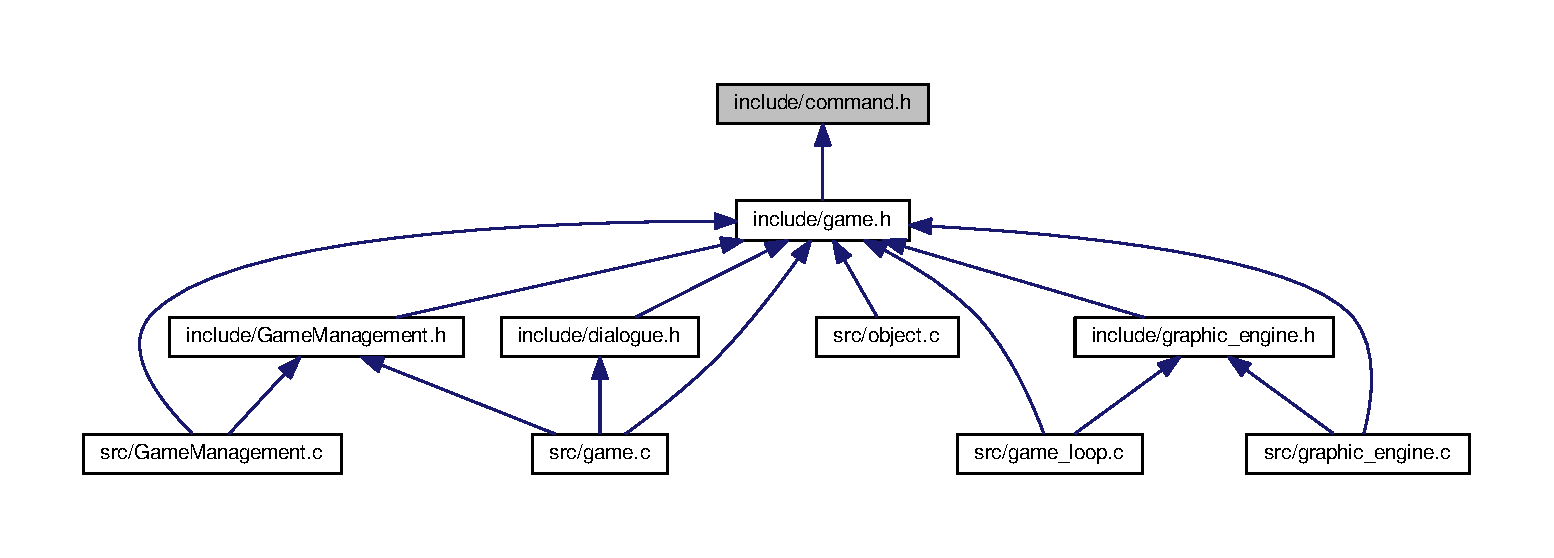
\includegraphics[width=350pt]{command_8h__dep__incl}
\end{center}
\end{figure}
\subsection*{Typedefs}
\begin{DoxyCompactItemize}
\item 
typedef enum \hyperlink{command_8h_ace19ba2296a74e4aef53304e0934c50c}{enum\+\_\+\+Command} \hyperlink{command_8h_a0473597db8c45c0289b6b8e2f8abbe32}{T\+\_\+\+Command}\hypertarget{command_8h_a0473597db8c45c0289b6b8e2f8abbe32}{}\label{command_8h_a0473597db8c45c0289b6b8e2f8abbe32}

\begin{DoxyCompactList}\small\item\em command list \end{DoxyCompactList}\end{DoxyCompactItemize}
\subsection*{Enumerations}
\begin{DoxyCompactItemize}
\item 
enum \hyperlink{command_8h_ace19ba2296a74e4aef53304e0934c50c}{enum\+\_\+\+Command} \{ \\*
\hyperlink{command_8h_ace19ba2296a74e4aef53304e0934c50ca785693a1d550a18688638e9124af41d0}{N\+O\+\_\+\+C\+MD} = -\/1, 
\hyperlink{command_8h_ace19ba2296a74e4aef53304e0934c50ca6ce26a62afab55d7606ad4e92428b30c}{U\+N\+K\+N\+O\+WN}, 
\hyperlink{command_8h_ace19ba2296a74e4aef53304e0934c50ca7a10b5d68d31711288e1fe0fa17dbf4f}{E\+X\+IT}, 
\hyperlink{command_8h_ace19ba2296a74e4aef53304e0934c50ca362b5ae0e519db264a4b2607d37d2a7e}{G\+R\+A\+SP}, 
\\*
\hyperlink{command_8h_ace19ba2296a74e4aef53304e0934c50ca8b0b0025af76a3d8f0b7b1d4758e51a6}{D\+R\+OP}, 
\hyperlink{command_8h_ace19ba2296a74e4aef53304e0934c50cabc5a79c786d2b239440dd3b92c402ef4}{T\+H\+R\+OW}, 
\hyperlink{command_8h_ace19ba2296a74e4aef53304e0934c50caed65b7dfe470f4e500b15f7074bb7fa2}{C\+H\+E\+CK}, 
\hyperlink{command_8h_ace19ba2296a74e4aef53304e0934c50caed3ef32890b6da0919b57254c5206c62}{M\+O\+VE}, 
\\*
\hyperlink{command_8h_ace19ba2296a74e4aef53304e0934c50ca141759a3bd88e1f969f53ce070705fcd}{T\+U\+R\+N\+ON}, 
\hyperlink{command_8h_ace19ba2296a74e4aef53304e0934c50ca564ee0e901bafdd34855cf0ad96ef60c}{T\+U\+R\+N\+O\+FF}, 
{\bfseries U\+N\+L\+O\+CK}, 
{\bfseries S\+A\+VE}, 
\\*
{\bfseries L\+O\+AD}
 \}\begin{DoxyCompactList}\small\item\em command list \end{DoxyCompactList}
\end{DoxyCompactItemize}
\subsection*{Functions}
\begin{DoxyCompactItemize}
\item 
\hyperlink{command_8h_a0473597db8c45c0289b6b8e2f8abbe32}{T\+\_\+\+Command} \hyperlink{command_8h_a7ad92506157db30fe6e1941d62752291}{command\+\_\+get\+\_\+user\+\_\+input} ()
\begin{DoxyCompactList}\small\item\em gets the command selected \end{DoxyCompactList}\end{DoxyCompactItemize}


\subsection{Detailed Description}
Contains the command list and the declaration of the get user input function. 

It is composed by the enumeration that lists all the commands available in the game. These are the actions that a player can make when playing the game.

\begin{DoxyAuthor}{Author}
Juan Moreno 
\end{DoxyAuthor}
\begin{DoxyVersion}{Version}
3.\+0 
\end{DoxyVersion}
\begin{DoxyDate}{Date}
07-\/04-\/2018 
\end{DoxyDate}


\subsection{Enumeration Type Documentation}
\index{command.\+h@{command.\+h}!enum\+\_\+\+Command@{enum\+\_\+\+Command}}
\index{enum\+\_\+\+Command@{enum\+\_\+\+Command}!command.\+h@{command.\+h}}
\subsubsection[{\texorpdfstring{enum\+\_\+\+Command}{enum_Command}}]{\setlength{\rightskip}{0pt plus 5cm}enum {\bf enum\+\_\+\+Command}}\hypertarget{command_8h_ace19ba2296a74e4aef53304e0934c50c}{}\label{command_8h_ace19ba2296a74e4aef53304e0934c50c}


command list 

\begin{Desc}
\item[Enumerator]\par
\begin{description}
\index{N\+O\+\_\+\+C\+MD@{N\+O\+\_\+\+C\+MD}!command.\+h@{command.\+h}}\index{command.\+h@{command.\+h}!N\+O\+\_\+\+C\+MD@{N\+O\+\_\+\+C\+MD}}\item[{\em 
N\+O\+\_\+\+C\+MD\hypertarget{command_8h_ace19ba2296a74e4aef53304e0934c50ca785693a1d550a18688638e9124af41d0}{}\label{command_8h_ace19ba2296a74e4aef53304e0934c50ca785693a1d550a18688638e9124af41d0}
}]error \index{U\+N\+K\+N\+O\+WN@{U\+N\+K\+N\+O\+WN}!command.\+h@{command.\+h}}\index{command.\+h@{command.\+h}!U\+N\+K\+N\+O\+WN@{U\+N\+K\+N\+O\+WN}}\item[{\em 
U\+N\+K\+N\+O\+WN\hypertarget{command_8h_ace19ba2296a74e4aef53304e0934c50ca6ce26a62afab55d7606ad4e92428b30c}{}\label{command_8h_ace19ba2296a74e4aef53304e0934c50ca6ce26a62afab55d7606ad4e92428b30c}
}]unknown command \index{E\+X\+IT@{E\+X\+IT}!command.\+h@{command.\+h}}\index{command.\+h@{command.\+h}!E\+X\+IT@{E\+X\+IT}}\item[{\em 
E\+X\+IT\hypertarget{command_8h_ace19ba2296a74e4aef53304e0934c50ca7a10b5d68d31711288e1fe0fa17dbf4f}{}\label{command_8h_ace19ba2296a74e4aef53304e0934c50ca7a10b5d68d31711288e1fe0fa17dbf4f}
}]exit command \index{G\+R\+A\+SP@{G\+R\+A\+SP}!command.\+h@{command.\+h}}\index{command.\+h@{command.\+h}!G\+R\+A\+SP@{G\+R\+A\+SP}}\item[{\em 
G\+R\+A\+SP\hypertarget{command_8h_ace19ba2296a74e4aef53304e0934c50ca362b5ae0e519db264a4b2607d37d2a7e}{}\label{command_8h_ace19ba2296a74e4aef53304e0934c50ca362b5ae0e519db264a4b2607d37d2a7e}
}]grasp command \index{D\+R\+OP@{D\+R\+OP}!command.\+h@{command.\+h}}\index{command.\+h@{command.\+h}!D\+R\+OP@{D\+R\+OP}}\item[{\em 
D\+R\+OP\hypertarget{command_8h_ace19ba2296a74e4aef53304e0934c50ca8b0b0025af76a3d8f0b7b1d4758e51a6}{}\label{command_8h_ace19ba2296a74e4aef53304e0934c50ca8b0b0025af76a3d8f0b7b1d4758e51a6}
}]drop command \index{T\+H\+R\+OW@{T\+H\+R\+OW}!command.\+h@{command.\+h}}\index{command.\+h@{command.\+h}!T\+H\+R\+OW@{T\+H\+R\+OW}}\item[{\em 
T\+H\+R\+OW\hypertarget{command_8h_ace19ba2296a74e4aef53304e0934c50cabc5a79c786d2b239440dd3b92c402ef4}{}\label{command_8h_ace19ba2296a74e4aef53304e0934c50cabc5a79c786d2b239440dd3b92c402ef4}
}]throw command \index{C\+H\+E\+CK@{C\+H\+E\+CK}!command.\+h@{command.\+h}}\index{command.\+h@{command.\+h}!C\+H\+E\+CK@{C\+H\+E\+CK}}\item[{\em 
C\+H\+E\+CK\hypertarget{command_8h_ace19ba2296a74e4aef53304e0934c50caed65b7dfe470f4e500b15f7074bb7fa2}{}\label{command_8h_ace19ba2296a74e4aef53304e0934c50caed65b7dfe470f4e500b15f7074bb7fa2}
}]check command \index{M\+O\+VE@{M\+O\+VE}!command.\+h@{command.\+h}}\index{command.\+h@{command.\+h}!M\+O\+VE@{M\+O\+VE}}\item[{\em 
M\+O\+VE\hypertarget{command_8h_ace19ba2296a74e4aef53304e0934c50caed3ef32890b6da0919b57254c5206c62}{}\label{command_8h_ace19ba2296a74e4aef53304e0934c50caed3ef32890b6da0919b57254c5206c62}
}]move command \index{T\+U\+R\+N\+ON@{T\+U\+R\+N\+ON}!command.\+h@{command.\+h}}\index{command.\+h@{command.\+h}!T\+U\+R\+N\+ON@{T\+U\+R\+N\+ON}}\item[{\em 
T\+U\+R\+N\+ON\hypertarget{command_8h_ace19ba2296a74e4aef53304e0934c50ca141759a3bd88e1f969f53ce070705fcd}{}\label{command_8h_ace19ba2296a74e4aef53304e0934c50ca141759a3bd88e1f969f53ce070705fcd}
}]swithcing on command \index{T\+U\+R\+N\+O\+FF@{T\+U\+R\+N\+O\+FF}!command.\+h@{command.\+h}}\index{command.\+h@{command.\+h}!T\+U\+R\+N\+O\+FF@{T\+U\+R\+N\+O\+FF}}\item[{\em 
T\+U\+R\+N\+O\+FF\hypertarget{command_8h_ace19ba2296a74e4aef53304e0934c50ca564ee0e901bafdd34855cf0ad96ef60c}{}\label{command_8h_ace19ba2296a74e4aef53304e0934c50ca564ee0e901bafdd34855cf0ad96ef60c}
}]swithcing off command \end{description}
\end{Desc}


\subsection{Function Documentation}
\index{command.\+h@{command.\+h}!command\+\_\+get\+\_\+user\+\_\+input@{command\+\_\+get\+\_\+user\+\_\+input}}
\index{command\+\_\+get\+\_\+user\+\_\+input@{command\+\_\+get\+\_\+user\+\_\+input}!command.\+h@{command.\+h}}
\subsubsection[{\texorpdfstring{command\+\_\+get\+\_\+user\+\_\+input()}{command_get_user_input()}}]{\setlength{\rightskip}{0pt plus 5cm}{\bf T\+\_\+\+Command} command\+\_\+get\+\_\+user\+\_\+input (
\begin{DoxyParamCaption}
{}
\end{DoxyParamCaption}
)}\hypertarget{command_8h_a7ad92506157db30fe6e1941d62752291}{}\label{command_8h_a7ad92506157db30fe6e1941d62752291}


gets the command selected 

Detects the command a user has written and converts it to a numerical code.

\begin{DoxyReturn}{Returns}
\hyperlink{command_8h_a0473597db8c45c0289b6b8e2f8abbe32}{T\+\_\+\+Command} ==$>$ Number from -\/1 to 9 with the command code. 
\end{DoxyReturn}

\hypertarget{dialogue_8h}{}\section{include/dialogue.h File Reference}
\label{dialogue_8h}\index{include/dialogue.\+h@{include/dialogue.\+h}}


Includes all the functionality used in the dialogue module.  


{\ttfamily \#include $<$stdio.\+h$>$}\\*
{\ttfamily \#include \char`\"{}game.\+h\char`\"{}}\\*
{\ttfamily \#include \char`\"{}types.\+h\char`\"{}}\\*
Include dependency graph for dialogue.\+h\+:
\nopagebreak
\begin{figure}[H]
\begin{center}
\leavevmode
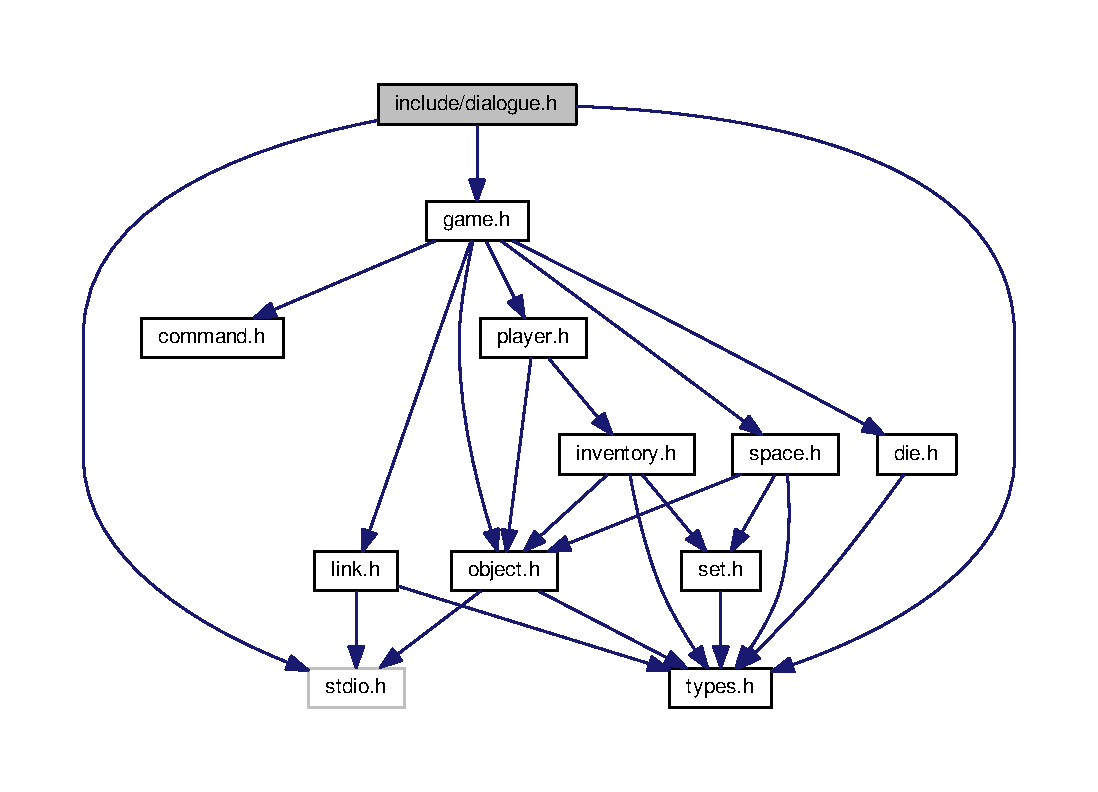
\includegraphics[width=350pt]{dialogue_8h__incl}
\end{center}
\end{figure}
This graph shows which files directly or indirectly include this file\+:
\nopagebreak
\begin{figure}[H]
\begin{center}
\leavevmode
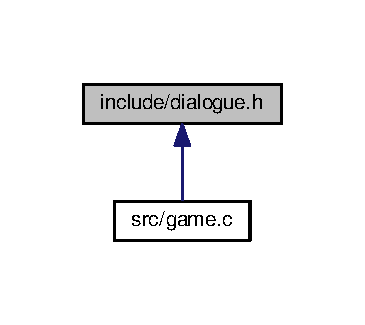
\includegraphics[width=175pt]{dialogue_8h__dep__incl}
\end{center}
\end{figure}
\subsection*{Functions}
\begin{DoxyCompactItemize}
\item 
char $\ast$ \hyperlink{dialogue_8h_ad069233c613ec944c257e638a784995c}{dialogue\+\_\+check\+\_\+space\+\_\+error} (\hyperlink{game_8h_a57156d39c530aec3fba3a9dad8c2dc6a}{Game} $\ast$game, \hyperlink{types_8h_a845e604fb28f7e3d97549da3448149d3}{Id} space)
\begin{DoxyCompactList}\small\item\em shows dialogue when error in spaces \end{DoxyCompactList}\item 
char $\ast$ \hyperlink{dialogue_8h_afa8c48c70f3237e9bda43359431fdfae}{dialogue\+\_\+check\+\_\+error} (char $\ast$oname)
\begin{DoxyCompactList}\small\item\em shows dialogue when error in spaces and objects \end{DoxyCompactList}\item 
char $\ast$ \hyperlink{dialogue_8h_a61a500ac7fd9354bcd02e6ea87bf004e}{dialogue\+\_\+check\+\_\+space\+\_\+success} (\hyperlink{game_8h_a57156d39c530aec3fba3a9dad8c2dc6a}{Game} $\ast$game, \hyperlink{types_8h_a845e604fb28f7e3d97549da3448149d3}{Id} space)
\begin{DoxyCompactList}\small\item\em shows dialogue when success in spaces \end{DoxyCompactList}\item 
char $\ast$ \hyperlink{dialogue_8h_adb5a55e8a732244ce0098876ba8d71e9}{dialogue\+\_\+movement\+\_\+success} (\hyperlink{game_8h_a57156d39c530aec3fba3a9dad8c2dc6a}{Game} $\ast$game, \hyperlink{types_8h_a845e604fb28f7e3d97549da3448149d3}{Id} space, char $\ast$cardinal)
\begin{DoxyCompactList}\small\item\em shows dialogue when success in movements \end{DoxyCompactList}\item 
char $\ast$ \hyperlink{dialogue_8h_a5e2d393f794a28c1599c82deebc86eec}{dialogue\+\_\+check\+\_\+object\+\_\+success} (\hyperlink{object_8h_a7f8bbcda919b65ce67f92fba08e0212f}{Object} $\ast$object)
\begin{DoxyCompactList}\small\item\em shows dialogue when success in checking an object \end{DoxyCompactList}\item 
char $\ast$ \hyperlink{dialogue_8h_a2afe0a62619498c4901bfad95623ca68}{dialogue\+\_\+movement\+\_\+error} (\hyperlink{game_8h_a57156d39c530aec3fba3a9dad8c2dc6a}{Game} $\ast$game, \hyperlink{types_8h_a845e604fb28f7e3d97549da3448149d3}{Id} space, char $\ast$cardinal)
\begin{DoxyCompactList}\small\item\em shows dialogue when error in movements \end{DoxyCompactList}\item 
char $\ast$ \hyperlink{dialogue_8h_afaccfa0802694861fd16d341f5fe0000}{dialogue\+\_\+throw\+\_\+die} (\hyperlink{die_8h_a892f0b0bf81d69a1f7a14ea238e36dd3}{Die} $\ast$die)
\begin{DoxyCompactList}\small\item\em shows dialogue when throwing the die \end{DoxyCompactList}\item 
char $\ast$ \hyperlink{dialogue_8h_a9bdc603b507386d5b571bff73e76446f}{dialogue\+\_\+drop\+\_\+object\+\_\+error} (char $\ast$oname, \hyperlink{game_8h_a57156d39c530aec3fba3a9dad8c2dc6a}{Game} $\ast$game, \hyperlink{types_8h_a845e604fb28f7e3d97549da3448149d3}{Id} act\+\_\+space, int j)
\begin{DoxyCompactList}\small\item\em shows dialogue when error while dropping an object \end{DoxyCompactList}\item 
char $\ast$ \hyperlink{dialogue_8h_a1a76549390e0e8fe0d995868d15d38ee}{dialogue\+\_\+drop\+\_\+object\+\_\+success} (\hyperlink{object_8h_a7f8bbcda919b65ce67f92fba08e0212f}{Object} $\ast$object, \hyperlink{game_8h_a57156d39c530aec3fba3a9dad8c2dc6a}{Game} $\ast$game, \hyperlink{types_8h_a845e604fb28f7e3d97549da3448149d3}{Id} act\+\_\+space)
\begin{DoxyCompactList}\small\item\em shows dialogue when success while dropping an object \end{DoxyCompactList}\item 
char $\ast$ \hyperlink{dialogue_8h_a1fa4917a65fd5b37d13b17de45c29e3d}{dialogue\+\_\+grasp\+\_\+object\+\_\+error} (char $\ast$oname, \hyperlink{game_8h_a57156d39c530aec3fba3a9dad8c2dc6a}{Game} $\ast$game, \hyperlink{types_8h_a845e604fb28f7e3d97549da3448149d3}{Id} act\+\_\+space, int j)
\begin{DoxyCompactList}\small\item\em shows dialogue when error while grasping an object \end{DoxyCompactList}\item 
char $\ast$ \hyperlink{dialogue_8h_a8ea8137ea45fcf20d2bc1f5d27a8860c}{dialogue\+\_\+grasp\+\_\+object\+\_\+success} (\hyperlink{object_8h_a7f8bbcda919b65ce67f92fba08e0212f}{Object} $\ast$object, \hyperlink{game_8h_a57156d39c530aec3fba3a9dad8c2dc6a}{Game} $\ast$game, \hyperlink{types_8h_a845e604fb28f7e3d97549da3448149d3}{Id} act\+\_\+space)
\begin{DoxyCompactList}\small\item\em shows dialogue when success while grasping an object \end{DoxyCompactList}\item 
char $\ast$ \hyperlink{dialogue_8h_adfed869e8fea0bac5b67f567f51ae95b}{dialogue\+\_\+unknown} ()
\begin{DoxyCompactList}\small\item\em shows dialogue when introducing an unknown command \end{DoxyCompactList}\item 
char $\ast$ \hyperlink{dialogue_8h_adaac05650dd4cc6312b3200c8cfbc5e3}{dialogue\+\_\+grasp\+\_\+object\+\_\+error\+\_\+movable} (char $\ast$oname, \hyperlink{game_8h_a57156d39c530aec3fba3a9dad8c2dc6a}{Game} $\ast$game, \hyperlink{types_8h_a845e604fb28f7e3d97549da3448149d3}{Id} space\+\_\+id)
\begin{DoxyCompactList}\small\item\em shows dialogue when error while grasping an object that is not movable \end{DoxyCompactList}\item 
char $\ast$ \hyperlink{dialogue_8h_a6a65260ade4162e962f190894dedd04a}{dialogue\+\_\+turnon\+\_\+object\+\_\+success} (char $\ast$oname)
\begin{DoxyCompactList}\small\item\em shows dialogue when success while turning on an object \end{DoxyCompactList}\item 
char $\ast$ \hyperlink{dialogue_8h_ab273e8bc8c74be3e695ddd0b20383535}{dialogue\+\_\+turnon\+\_\+object\+\_\+error} (char $\ast$oname, int j, int k)
\begin{DoxyCompactList}\small\item\em shows dialogue when error while turning on an object \end{DoxyCompactList}\item 
char $\ast$ \hyperlink{dialogue_8h_a03bb4bcb30b096b81c60e18c6727c6e0}{dialogue\+\_\+turnoff\+\_\+object\+\_\+success} (char $\ast$oname)
\begin{DoxyCompactList}\small\item\em shows dialogue when success while turning off an object \end{DoxyCompactList}\item 
char $\ast$ \hyperlink{dialogue_8h_a50e5a6b2c821cea158ceada240c542d6}{dialogue\+\_\+turnoff\+\_\+object\+\_\+error} (char $\ast$oname, int j)
\begin{DoxyCompactList}\small\item\em shows dialogue when error while turning off an object \end{DoxyCompactList}\item 
char $\ast$ \hyperlink{dialogue_8h_a2bd7ede8cc08a3a5dbac38f1990de814}{dialogue\+\_\+unlock\+\_\+success} (char $\ast$object, char $\ast$link)
\begin{DoxyCompactList}\small\item\em shows dialogue when success while unlocking a door \end{DoxyCompactList}\item 
char $\ast$ \hyperlink{dialogue_8h_a992dfad74514a3fe7dfe081b993aca95}{dialogue\+\_\+unlock\+\_\+error} (char $\ast$object, char $\ast$link, int j, int k)
\begin{DoxyCompactList}\small\item\em shows dialogue when error while unlocking a door \end{DoxyCompactList}\item 
char $\ast$ \hyperlink{dialogue_8h_ace7e6623bd79b3e3d9dc5f65f278776a}{dialogue\+\_\+movement\+\_\+link\+\_\+error} (\hyperlink{game_8h_a57156d39c530aec3fba3a9dad8c2dc6a}{Game} $\ast$game, \hyperlink{types_8h_a845e604fb28f7e3d97549da3448149d3}{Id} space, char $\ast$cardinal)
\begin{DoxyCompactList}\small\item\em shows dialogue when error while moving \end{DoxyCompactList}\end{DoxyCompactItemize}


\subsection{Detailed Description}
Includes all the functionality used in the dialogue module. 

\begin{DoxyAuthor}{Author}
Andrés Mena 
\end{DoxyAuthor}
\begin{DoxyVersion}{Version}
1.\+0 
\end{DoxyVersion}
\begin{DoxyDate}{Date}
29-\/04-\/2018 
\end{DoxyDate}


\subsection{Function Documentation}
\index{dialogue.\+h@{dialogue.\+h}!dialogue\+\_\+check\+\_\+error@{dialogue\+\_\+check\+\_\+error}}
\index{dialogue\+\_\+check\+\_\+error@{dialogue\+\_\+check\+\_\+error}!dialogue.\+h@{dialogue.\+h}}
\subsubsection[{\texorpdfstring{dialogue\+\_\+check\+\_\+error(char $\ast$oname)}{dialogue_check_error(char *oname)}}]{\setlength{\rightskip}{0pt plus 5cm}char$\ast$ dialogue\+\_\+check\+\_\+error (
\begin{DoxyParamCaption}
\item[{char $\ast$}]{oname}
\end{DoxyParamCaption}
)}\hypertarget{dialogue_8h_afa8c48c70f3237e9bda43359431fdfae}{}\label{dialogue_8h_afa8c48c70f3237e9bda43359431fdfae}


shows dialogue when error in spaces and objects 

Checks if there is an error in the location of spaces and objects.

\begin{DoxyAuthor}{Author}
Andrés Mena 
\end{DoxyAuthor}

\begin{DoxyParams}{Parameters}
{\em oname} & (pointer to char). \\
\hline
\end{DoxyParams}
\begin{DoxyReturn}{Returns}
pointer to char (string of characters that shows a message if there is an error). 
\end{DoxyReturn}
\index{dialogue.\+h@{dialogue.\+h}!dialogue\+\_\+check\+\_\+object\+\_\+success@{dialogue\+\_\+check\+\_\+object\+\_\+success}}
\index{dialogue\+\_\+check\+\_\+object\+\_\+success@{dialogue\+\_\+check\+\_\+object\+\_\+success}!dialogue.\+h@{dialogue.\+h}}
\subsubsection[{\texorpdfstring{dialogue\+\_\+check\+\_\+object\+\_\+success(\+Object $\ast$object)}{dialogue_check_object_success(Object *object)}}]{\setlength{\rightskip}{0pt plus 5cm}char$\ast$ dialogue\+\_\+check\+\_\+object\+\_\+success (
\begin{DoxyParamCaption}
\item[{{\bf Object} $\ast$}]{object}
\end{DoxyParamCaption}
)}\hypertarget{dialogue_8h_a5e2d393f794a28c1599c82deebc86eec}{}\label{dialogue_8h_a5e2d393f794a28c1599c82deebc86eec}


shows dialogue when success in checking an object 

Checks the position of an object and shows a message either it is in its original position or not.

\begin{DoxyAuthor}{Author}
Andrés Mena 
\end{DoxyAuthor}

\begin{DoxyParams}{Parameters}
{\em object} & pointer to object. \\
\hline
\end{DoxyParams}
\begin{DoxyReturn}{Returns}
pointer to char (string of characters that shows a message if there is success). 
\end{DoxyReturn}
\index{dialogue.\+h@{dialogue.\+h}!dialogue\+\_\+check\+\_\+space\+\_\+error@{dialogue\+\_\+check\+\_\+space\+\_\+error}}
\index{dialogue\+\_\+check\+\_\+space\+\_\+error@{dialogue\+\_\+check\+\_\+space\+\_\+error}!dialogue.\+h@{dialogue.\+h}}
\subsubsection[{\texorpdfstring{dialogue\+\_\+check\+\_\+space\+\_\+error(\+Game $\ast$game, Id space)}{dialogue_check_space_error(Game *game, Id space)}}]{\setlength{\rightskip}{0pt plus 5cm}char$\ast$ dialogue\+\_\+check\+\_\+space\+\_\+error (
\begin{DoxyParamCaption}
\item[{{\bf Game} $\ast$}]{game, }
\item[{{\bf Id}}]{space}
\end{DoxyParamCaption}
)}\hypertarget{dialogue_8h_ad069233c613ec944c257e638a784995c}{}\label{dialogue_8h_ad069233c613ec944c257e638a784995c}


shows dialogue when error in spaces 

Checks if there is an error in the space that the player wants to interact with.

\begin{DoxyAuthor}{Author}
Andrés Mena 
\end{DoxyAuthor}

\begin{DoxyParams}{Parameters}
{\em game} & pointer to game. \\
\hline
{\em space} & Id (long int). \\
\hline
\end{DoxyParams}
\begin{DoxyReturn}{Returns}
pointer to char (string of characters that shows a message if there is an error). 
\end{DoxyReturn}
\index{dialogue.\+h@{dialogue.\+h}!dialogue\+\_\+check\+\_\+space\+\_\+success@{dialogue\+\_\+check\+\_\+space\+\_\+success}}
\index{dialogue\+\_\+check\+\_\+space\+\_\+success@{dialogue\+\_\+check\+\_\+space\+\_\+success}!dialogue.\+h@{dialogue.\+h}}
\subsubsection[{\texorpdfstring{dialogue\+\_\+check\+\_\+space\+\_\+success(\+Game $\ast$game, Id space)}{dialogue_check_space_success(Game *game, Id space)}}]{\setlength{\rightskip}{0pt plus 5cm}char$\ast$ dialogue\+\_\+check\+\_\+space\+\_\+success (
\begin{DoxyParamCaption}
\item[{{\bf Game} $\ast$}]{game, }
\item[{{\bf Id}}]{space}
\end{DoxyParamCaption}
)}\hypertarget{dialogue_8h_a61a500ac7fd9354bcd02e6ea87bf004e}{}\label{dialogue_8h_a61a500ac7fd9354bcd02e6ea87bf004e}


shows dialogue when success in spaces 

Checks if there is something wrong with the space you want to interact with and shows a message if there is no error.

\begin{DoxyAuthor}{Author}
Andrés Mena 
\end{DoxyAuthor}

\begin{DoxyParams}{Parameters}
{\em game} & pointer to game. \\
\hline
{\em space} & Id (long int). \\
\hline
\end{DoxyParams}
\begin{DoxyReturn}{Returns}
pointer to char (string of characters that shows a message if there is success). 
\end{DoxyReturn}
\index{dialogue.\+h@{dialogue.\+h}!dialogue\+\_\+drop\+\_\+object\+\_\+error@{dialogue\+\_\+drop\+\_\+object\+\_\+error}}
\index{dialogue\+\_\+drop\+\_\+object\+\_\+error@{dialogue\+\_\+drop\+\_\+object\+\_\+error}!dialogue.\+h@{dialogue.\+h}}
\subsubsection[{\texorpdfstring{dialogue\+\_\+drop\+\_\+object\+\_\+error(char $\ast$oname, Game $\ast$game, Id act\+\_\+space, int j)}{dialogue_drop_object_error(char *oname, Game *game, Id act_space, int j)}}]{\setlength{\rightskip}{0pt plus 5cm}char$\ast$ dialogue\+\_\+drop\+\_\+object\+\_\+error (
\begin{DoxyParamCaption}
\item[{char $\ast$}]{oname, }
\item[{{\bf Game} $\ast$}]{game, }
\item[{{\bf Id}}]{act\+\_\+space, }
\item[{int}]{j}
\end{DoxyParamCaption}
)}\hypertarget{dialogue_8h_a9bdc603b507386d5b571bff73e76446f}{}\label{dialogue_8h_a9bdc603b507386d5b571bff73e76446f}


shows dialogue when error while dropping an object 

Checks if there is an error when trying to drop an object and shows a message.

\begin{DoxyAuthor}{Author}
Andrés Mena 
\end{DoxyAuthor}

\begin{DoxyParams}{Parameters}
{\em oname} & pointer to char. \\
\hline
{\em game} & pointer to game. \\
\hline
{\em act\+\_\+space} & Id (long int). \\
\hline
{\em j} & (int value). \\
\hline
\end{DoxyParams}
\begin{DoxyReturn}{Returns}
pointer to char (string of characters that shows a message if there is an error). 
\end{DoxyReturn}
\index{dialogue.\+h@{dialogue.\+h}!dialogue\+\_\+drop\+\_\+object\+\_\+success@{dialogue\+\_\+drop\+\_\+object\+\_\+success}}
\index{dialogue\+\_\+drop\+\_\+object\+\_\+success@{dialogue\+\_\+drop\+\_\+object\+\_\+success}!dialogue.\+h@{dialogue.\+h}}
\subsubsection[{\texorpdfstring{dialogue\+\_\+drop\+\_\+object\+\_\+success(\+Object $\ast$object, Game $\ast$game, Id act\+\_\+space)}{dialogue_drop_object_success(Object *object, Game *game, Id act_space)}}]{\setlength{\rightskip}{0pt plus 5cm}char$\ast$ dialogue\+\_\+drop\+\_\+object\+\_\+success (
\begin{DoxyParamCaption}
\item[{{\bf Object} $\ast$}]{object, }
\item[{{\bf Game} $\ast$}]{game, }
\item[{{\bf Id}}]{act\+\_\+space}
\end{DoxyParamCaption}
)}\hypertarget{dialogue_8h_a1a76549390e0e8fe0d995868d15d38ee}{}\label{dialogue_8h_a1a76549390e0e8fe0d995868d15d38ee}


shows dialogue when success while dropping an object 

Checks if there is an error when trying to drop an object and shows a message if the object has been dropped succesfully.

\begin{DoxyAuthor}{Author}
Andrés Mena 
\end{DoxyAuthor}

\begin{DoxyParams}{Parameters}
{\em object} & pointer to object. \\
\hline
{\em game} & pointer to game. \\
\hline
{\em act\+\_\+space} & Id (long int). \\
\hline
\end{DoxyParams}
\begin{DoxyReturn}{Returns}
pointer to char (string of characters that shows a message if there is success). 
\end{DoxyReturn}
\index{dialogue.\+h@{dialogue.\+h}!dialogue\+\_\+grasp\+\_\+object\+\_\+error@{dialogue\+\_\+grasp\+\_\+object\+\_\+error}}
\index{dialogue\+\_\+grasp\+\_\+object\+\_\+error@{dialogue\+\_\+grasp\+\_\+object\+\_\+error}!dialogue.\+h@{dialogue.\+h}}
\subsubsection[{\texorpdfstring{dialogue\+\_\+grasp\+\_\+object\+\_\+error(char $\ast$oname, Game $\ast$game, Id act\+\_\+space, int j)}{dialogue_grasp_object_error(char *oname, Game *game, Id act_space, int j)}}]{\setlength{\rightskip}{0pt plus 5cm}char$\ast$ dialogue\+\_\+grasp\+\_\+object\+\_\+error (
\begin{DoxyParamCaption}
\item[{char $\ast$}]{oname, }
\item[{{\bf Game} $\ast$}]{game, }
\item[{{\bf Id}}]{act\+\_\+space, }
\item[{int}]{j}
\end{DoxyParamCaption}
)}\hypertarget{dialogue_8h_a1fa4917a65fd5b37d13b17de45c29e3d}{}\label{dialogue_8h_a1fa4917a65fd5b37d13b17de45c29e3d}


shows dialogue when error while grasping an object 

Checks if there is an error when trying to grasp an object and shows a message.

\begin{DoxyAuthor}{Author}
Andrés Mena 
\end{DoxyAuthor}

\begin{DoxyParams}{Parameters}
{\em oname} & pointer to char. \\
\hline
{\em game} & pointer to game. \\
\hline
{\em act\+\_\+space} & Id (long int). \\
\hline
{\em j} & (int value). \\
\hline
\end{DoxyParams}
\begin{DoxyReturn}{Returns}
pointer to char (string of characters that shows a message if there is an error). 
\end{DoxyReturn}
\index{dialogue.\+h@{dialogue.\+h}!dialogue\+\_\+grasp\+\_\+object\+\_\+error\+\_\+movable@{dialogue\+\_\+grasp\+\_\+object\+\_\+error\+\_\+movable}}
\index{dialogue\+\_\+grasp\+\_\+object\+\_\+error\+\_\+movable@{dialogue\+\_\+grasp\+\_\+object\+\_\+error\+\_\+movable}!dialogue.\+h@{dialogue.\+h}}
\subsubsection[{\texorpdfstring{dialogue\+\_\+grasp\+\_\+object\+\_\+error\+\_\+movable(char $\ast$oname, Game $\ast$game, Id space\+\_\+id)}{dialogue_grasp_object_error_movable(char *oname, Game *game, Id space_id)}}]{\setlength{\rightskip}{0pt plus 5cm}char$\ast$ dialogue\+\_\+grasp\+\_\+object\+\_\+error\+\_\+movable (
\begin{DoxyParamCaption}
\item[{char $\ast$}]{oname, }
\item[{{\bf Game} $\ast$}]{game, }
\item[{{\bf Id}}]{space\+\_\+id}
\end{DoxyParamCaption}
)}\hypertarget{dialogue_8h_adaac05650dd4cc6312b3200c8cfbc5e3}{}\label{dialogue_8h_adaac05650dd4cc6312b3200c8cfbc5e3}


shows dialogue when error while grasping an object that is not movable 

Checks if there is an error when trying to grasp a non-\/movable object and shows a message.

\begin{DoxyAuthor}{Author}
Andrés Mena 
\end{DoxyAuthor}

\begin{DoxyParams}{Parameters}
{\em oname} & pointer to char. \\
\hline
{\em game} & pointer to game. \\
\hline
{\em space\+\_\+id} & Id (long int). \\
\hline
\end{DoxyParams}
\begin{DoxyReturn}{Returns}
pointer to char (string of characters that shows a message if there is an error). 
\end{DoxyReturn}
\index{dialogue.\+h@{dialogue.\+h}!dialogue\+\_\+grasp\+\_\+object\+\_\+success@{dialogue\+\_\+grasp\+\_\+object\+\_\+success}}
\index{dialogue\+\_\+grasp\+\_\+object\+\_\+success@{dialogue\+\_\+grasp\+\_\+object\+\_\+success}!dialogue.\+h@{dialogue.\+h}}
\subsubsection[{\texorpdfstring{dialogue\+\_\+grasp\+\_\+object\+\_\+success(\+Object $\ast$object, Game $\ast$game, Id act\+\_\+space)}{dialogue_grasp_object_success(Object *object, Game *game, Id act_space)}}]{\setlength{\rightskip}{0pt plus 5cm}char$\ast$ dialogue\+\_\+grasp\+\_\+object\+\_\+success (
\begin{DoxyParamCaption}
\item[{{\bf Object} $\ast$}]{object, }
\item[{{\bf Game} $\ast$}]{game, }
\item[{{\bf Id}}]{act\+\_\+space}
\end{DoxyParamCaption}
)}\hypertarget{dialogue_8h_a8ea8137ea45fcf20d2bc1f5d27a8860c}{}\label{dialogue_8h_a8ea8137ea45fcf20d2bc1f5d27a8860c}


shows dialogue when success while grasping an object 

Checks if there is an error when trying to grasp an object and shows a message if the object has been grasped succesfully.

\begin{DoxyAuthor}{Author}
Andrés Mena 
\end{DoxyAuthor}

\begin{DoxyParams}{Parameters}
{\em object} & pointer to object. \\
\hline
{\em game} & pointer to game. \\
\hline
{\em act\+\_\+space} & Id (long int). \\
\hline
\end{DoxyParams}
\begin{DoxyReturn}{Returns}
pointer to char (string of characters that shows a message if there is success). 
\end{DoxyReturn}
\index{dialogue.\+h@{dialogue.\+h}!dialogue\+\_\+movement\+\_\+error@{dialogue\+\_\+movement\+\_\+error}}
\index{dialogue\+\_\+movement\+\_\+error@{dialogue\+\_\+movement\+\_\+error}!dialogue.\+h@{dialogue.\+h}}
\subsubsection[{\texorpdfstring{dialogue\+\_\+movement\+\_\+error(\+Game $\ast$game, Id space, char $\ast$cardinal)}{dialogue_movement_error(Game *game, Id space, char *cardinal)}}]{\setlength{\rightskip}{0pt plus 5cm}char$\ast$ dialogue\+\_\+movement\+\_\+error (
\begin{DoxyParamCaption}
\item[{{\bf Game} $\ast$}]{game, }
\item[{{\bf Id}}]{space, }
\item[{char $\ast$}]{cardinal}
\end{DoxyParamCaption}
)}\hypertarget{dialogue_8h_a2afe0a62619498c4901bfad95623ca68}{}\label{dialogue_8h_a2afe0a62619498c4901bfad95623ca68}


shows dialogue when error in movements 

Checks the different movements and shows a message that tells the player that the movement is not allowed if there is an error while checking the movement.

\begin{DoxyAuthor}{Author}
Andrés Mena 
\end{DoxyAuthor}

\begin{DoxyParams}{Parameters}
{\em game} & pointer to game. \\
\hline
{\em space} & Id (long int). \\
\hline
{\em cardinal} & (char). \\
\hline
\end{DoxyParams}
\begin{DoxyReturn}{Returns}
pointer to char (string of characters that shows a message if there is an error). 
\end{DoxyReturn}
\index{dialogue.\+h@{dialogue.\+h}!dialogue\+\_\+movement\+\_\+link\+\_\+error@{dialogue\+\_\+movement\+\_\+link\+\_\+error}}
\index{dialogue\+\_\+movement\+\_\+link\+\_\+error@{dialogue\+\_\+movement\+\_\+link\+\_\+error}!dialogue.\+h@{dialogue.\+h}}
\subsubsection[{\texorpdfstring{dialogue\+\_\+movement\+\_\+link\+\_\+error(\+Game $\ast$game, Id space, char $\ast$cardinal)}{dialogue_movement_link_error(Game *game, Id space, char *cardinal)}}]{\setlength{\rightskip}{0pt plus 5cm}char$\ast$ dialogue\+\_\+movement\+\_\+link\+\_\+error (
\begin{DoxyParamCaption}
\item[{{\bf Game} $\ast$}]{game, }
\item[{{\bf Id}}]{space, }
\item[{char $\ast$}]{cardinal}
\end{DoxyParamCaption}
)}\hypertarget{dialogue_8h_ace7e6623bd79b3e3d9dc5f65f278776a}{}\label{dialogue_8h_ace7e6623bd79b3e3d9dc5f65f278776a}


shows dialogue when error while moving 

Checks if there is an error when trying to make a move

\begin{DoxyAuthor}{Author}
Andrés Mena 
\end{DoxyAuthor}

\begin{DoxyParams}{Parameters}
{\em game} & pointer to game. \\
\hline
{\em space} & long int \\
\hline
{\em cardinal} & pointer to char \\
\hline
\end{DoxyParams}
\begin{DoxyReturn}{Returns}
pointer to char (string of characters that shows a message if there is an error). 
\end{DoxyReturn}
\index{dialogue.\+h@{dialogue.\+h}!dialogue\+\_\+movement\+\_\+success@{dialogue\+\_\+movement\+\_\+success}}
\index{dialogue\+\_\+movement\+\_\+success@{dialogue\+\_\+movement\+\_\+success}!dialogue.\+h@{dialogue.\+h}}
\subsubsection[{\texorpdfstring{dialogue\+\_\+movement\+\_\+success(\+Game $\ast$game, Id space, char $\ast$cardinal)}{dialogue_movement_success(Game *game, Id space, char *cardinal)}}]{\setlength{\rightskip}{0pt plus 5cm}char$\ast$ dialogue\+\_\+movement\+\_\+success (
\begin{DoxyParamCaption}
\item[{{\bf Game} $\ast$}]{game, }
\item[{{\bf Id}}]{space, }
\item[{char $\ast$}]{cardinal}
\end{DoxyParamCaption}
)}\hypertarget{dialogue_8h_adb5a55e8a732244ce0098876ba8d71e9}{}\label{dialogue_8h_adb5a55e8a732244ce0098876ba8d71e9}


shows dialogue when success in movements 

Checks the different movements and shows a message that describes where have you been moved and the name of the space.

\begin{DoxyAuthor}{Author}
Andrés Mena 
\end{DoxyAuthor}

\begin{DoxyParams}{Parameters}
{\em game} & pointer to game. \\
\hline
{\em space} & Id (long int). \\
\hline
{\em cardinal} & (char). \\
\hline
\end{DoxyParams}
\begin{DoxyReturn}{Returns}
pointer to char (string of characters that shows a message if there is success). 
\end{DoxyReturn}
\index{dialogue.\+h@{dialogue.\+h}!dialogue\+\_\+throw\+\_\+die@{dialogue\+\_\+throw\+\_\+die}}
\index{dialogue\+\_\+throw\+\_\+die@{dialogue\+\_\+throw\+\_\+die}!dialogue.\+h@{dialogue.\+h}}
\subsubsection[{\texorpdfstring{dialogue\+\_\+throw\+\_\+die(\+Die $\ast$die)}{dialogue_throw_die(Die *die)}}]{\setlength{\rightskip}{0pt plus 5cm}char$\ast$ dialogue\+\_\+throw\+\_\+die (
\begin{DoxyParamCaption}
\item[{{\bf Die} $\ast$}]{die}
\end{DoxyParamCaption}
)}\hypertarget{dialogue_8h_afaccfa0802694861fd16d341f5fe0000}{}\label{dialogue_8h_afaccfa0802694861fd16d341f5fe0000}


shows dialogue when throwing the die 

Checks if there is any error with the die and shows a message with the value of the die.

\begin{DoxyAuthor}{Author}
Andrés Mena 
\end{DoxyAuthor}

\begin{DoxyParams}{Parameters}
{\em die} & pointer do Die. \\
\hline
\end{DoxyParams}
\begin{DoxyReturn}{Returns}
pointer to char (string of characters that shows a message when throwing the die). 
\end{DoxyReturn}
\index{dialogue.\+h@{dialogue.\+h}!dialogue\+\_\+turnoff\+\_\+object\+\_\+error@{dialogue\+\_\+turnoff\+\_\+object\+\_\+error}}
\index{dialogue\+\_\+turnoff\+\_\+object\+\_\+error@{dialogue\+\_\+turnoff\+\_\+object\+\_\+error}!dialogue.\+h@{dialogue.\+h}}
\subsubsection[{\texorpdfstring{dialogue\+\_\+turnoff\+\_\+object\+\_\+error(char $\ast$oname, int j)}{dialogue_turnoff_object_error(char *oname, int j)}}]{\setlength{\rightskip}{0pt plus 5cm}char$\ast$ dialogue\+\_\+turnoff\+\_\+object\+\_\+error (
\begin{DoxyParamCaption}
\item[{char $\ast$}]{oname, }
\item[{int}]{j}
\end{DoxyParamCaption}
)}\hypertarget{dialogue_8h_a50e5a6b2c821cea158ceada240c542d6}{}\label{dialogue_8h_a50e5a6b2c821cea158ceada240c542d6}


shows dialogue when error while turning off an object 

Checks if there is an error when trying to turn off an object and shows a message.

\begin{DoxyAuthor}{Author}
Andrés Mena 
\end{DoxyAuthor}

\begin{DoxyParams}{Parameters}
{\em oname} & pointer to char. \\
\hline
{\em j} & (int value). \\
\hline
\end{DoxyParams}
\begin{DoxyReturn}{Returns}
pointer to char (string of characters that shows a message if there is an error). 
\end{DoxyReturn}
\index{dialogue.\+h@{dialogue.\+h}!dialogue\+\_\+turnoff\+\_\+object\+\_\+success@{dialogue\+\_\+turnoff\+\_\+object\+\_\+success}}
\index{dialogue\+\_\+turnoff\+\_\+object\+\_\+success@{dialogue\+\_\+turnoff\+\_\+object\+\_\+success}!dialogue.\+h@{dialogue.\+h}}
\subsubsection[{\texorpdfstring{dialogue\+\_\+turnoff\+\_\+object\+\_\+success(char $\ast$oname)}{dialogue_turnoff_object_success(char *oname)}}]{\setlength{\rightskip}{0pt plus 5cm}char$\ast$ dialogue\+\_\+turnoff\+\_\+object\+\_\+success (
\begin{DoxyParamCaption}
\item[{char $\ast$}]{oname}
\end{DoxyParamCaption}
)}\hypertarget{dialogue_8h_a03bb4bcb30b096b81c60e18c6727c6e0}{}\label{dialogue_8h_a03bb4bcb30b096b81c60e18c6727c6e0}


shows dialogue when success while turning off an object 

Checks if there is an error when trying to turn off an object and shows a message if the object has been turned off succesfully.

\begin{DoxyAuthor}{Author}
Andrés Mena 
\end{DoxyAuthor}

\begin{DoxyParams}{Parameters}
{\em oname} & pointer to char. \\
\hline
\end{DoxyParams}
\begin{DoxyReturn}{Returns}
pointer to char (string of characters that shows a message if there is success). 
\end{DoxyReturn}
\index{dialogue.\+h@{dialogue.\+h}!dialogue\+\_\+turnon\+\_\+object\+\_\+error@{dialogue\+\_\+turnon\+\_\+object\+\_\+error}}
\index{dialogue\+\_\+turnon\+\_\+object\+\_\+error@{dialogue\+\_\+turnon\+\_\+object\+\_\+error}!dialogue.\+h@{dialogue.\+h}}
\subsubsection[{\texorpdfstring{dialogue\+\_\+turnon\+\_\+object\+\_\+error(char $\ast$oname, int j, int k)}{dialogue_turnon_object_error(char *oname, int j, int k)}}]{\setlength{\rightskip}{0pt plus 5cm}char$\ast$ dialogue\+\_\+turnon\+\_\+object\+\_\+error (
\begin{DoxyParamCaption}
\item[{char $\ast$}]{oname, }
\item[{int}]{j, }
\item[{int}]{k}
\end{DoxyParamCaption}
)}\hypertarget{dialogue_8h_ab273e8bc8c74be3e695ddd0b20383535}{}\label{dialogue_8h_ab273e8bc8c74be3e695ddd0b20383535}


shows dialogue when error while turning on an object 

Checks if there is an error when trying to turn on an object and shows a message.

\begin{DoxyAuthor}{Author}
Andrés Mena 
\end{DoxyAuthor}

\begin{DoxyParams}{Parameters}
{\em oname} & pointer to char. \\
\hline
{\em j} & (int value). \\
\hline
{\em k} & (int value). \\
\hline
\end{DoxyParams}
\begin{DoxyReturn}{Returns}
pointer to char (string of characters that shows a message if there is an error). 
\end{DoxyReturn}
\index{dialogue.\+h@{dialogue.\+h}!dialogue\+\_\+turnon\+\_\+object\+\_\+success@{dialogue\+\_\+turnon\+\_\+object\+\_\+success}}
\index{dialogue\+\_\+turnon\+\_\+object\+\_\+success@{dialogue\+\_\+turnon\+\_\+object\+\_\+success}!dialogue.\+h@{dialogue.\+h}}
\subsubsection[{\texorpdfstring{dialogue\+\_\+turnon\+\_\+object\+\_\+success(char $\ast$oname)}{dialogue_turnon_object_success(char *oname)}}]{\setlength{\rightskip}{0pt plus 5cm}char$\ast$ dialogue\+\_\+turnon\+\_\+object\+\_\+success (
\begin{DoxyParamCaption}
\item[{char $\ast$}]{oname}
\end{DoxyParamCaption}
)}\hypertarget{dialogue_8h_a6a65260ade4162e962f190894dedd04a}{}\label{dialogue_8h_a6a65260ade4162e962f190894dedd04a}


shows dialogue when success while turning on an object 

Checks if there is an error when trying to turn on an object and shows a message if the object has been turned on succesfully.

\begin{DoxyAuthor}{Author}
Andrés Mena 
\end{DoxyAuthor}

\begin{DoxyParams}{Parameters}
{\em oname} & pointer to char. \\
\hline
\end{DoxyParams}
\begin{DoxyReturn}{Returns}
pointer to char (string of characters that shows a message if there is success). 
\end{DoxyReturn}
\index{dialogue.\+h@{dialogue.\+h}!dialogue\+\_\+unknown@{dialogue\+\_\+unknown}}
\index{dialogue\+\_\+unknown@{dialogue\+\_\+unknown}!dialogue.\+h@{dialogue.\+h}}
\subsubsection[{\texorpdfstring{dialogue\+\_\+unknown()}{dialogue_unknown()}}]{\setlength{\rightskip}{0pt plus 5cm}char$\ast$ dialogue\+\_\+unknown (
\begin{DoxyParamCaption}
{}
\end{DoxyParamCaption}
)}\hypertarget{dialogue_8h_adfed869e8fea0bac5b67f567f51ae95b}{}\label{dialogue_8h_adfed869e8fea0bac5b67f567f51ae95b}


shows dialogue when introducing an unknown command 

Checks if there is an error while introducing a command and shows an error message.

\begin{DoxyAuthor}{Author}
Andrés Mena 
\end{DoxyAuthor}
\begin{DoxyReturn}{Returns}
pointer to char (string of characters that shows a message if the command is unknown). 
\end{DoxyReturn}
\index{dialogue.\+h@{dialogue.\+h}!dialogue\+\_\+unlock\+\_\+error@{dialogue\+\_\+unlock\+\_\+error}}
\index{dialogue\+\_\+unlock\+\_\+error@{dialogue\+\_\+unlock\+\_\+error}!dialogue.\+h@{dialogue.\+h}}
\subsubsection[{\texorpdfstring{dialogue\+\_\+unlock\+\_\+error(char $\ast$object, char $\ast$link, int j, int k)}{dialogue_unlock_error(char *object, char *link, int j, int k)}}]{\setlength{\rightskip}{0pt plus 5cm}char$\ast$ dialogue\+\_\+unlock\+\_\+error (
\begin{DoxyParamCaption}
\item[{char $\ast$}]{object, }
\item[{char $\ast$}]{link, }
\item[{int}]{j, }
\item[{int}]{k}
\end{DoxyParamCaption}
)}\hypertarget{dialogue_8h_a992dfad74514a3fe7dfe081b993aca95}{}\label{dialogue_8h_a992dfad74514a3fe7dfe081b993aca95}


shows dialogue when error while unlocking a door 

Checks if there is an error when trying to unlock a door shows a message

\begin{DoxyAuthor}{Author}
Andrés Mena 
\end{DoxyAuthor}

\begin{DoxyParams}{Parameters}
{\em object} & pointer to char. \\
\hline
{\em link} & pointer to char. \\
\hline
{\em j} & (int value). \\
\hline
{\em k} & (int value). \\
\hline
\end{DoxyParams}
\begin{DoxyReturn}{Returns}
pointer to char (string of characters that shows a message if there is an error). 
\end{DoxyReturn}
\index{dialogue.\+h@{dialogue.\+h}!dialogue\+\_\+unlock\+\_\+success@{dialogue\+\_\+unlock\+\_\+success}}
\index{dialogue\+\_\+unlock\+\_\+success@{dialogue\+\_\+unlock\+\_\+success}!dialogue.\+h@{dialogue.\+h}}
\subsubsection[{\texorpdfstring{dialogue\+\_\+unlock\+\_\+success(char $\ast$object, char $\ast$link)}{dialogue_unlock_success(char *object, char *link)}}]{\setlength{\rightskip}{0pt plus 5cm}char$\ast$ dialogue\+\_\+unlock\+\_\+success (
\begin{DoxyParamCaption}
\item[{char $\ast$}]{object, }
\item[{char $\ast$}]{link}
\end{DoxyParamCaption}
)}\hypertarget{dialogue_8h_a2bd7ede8cc08a3a5dbac38f1990de814}{}\label{dialogue_8h_a2bd7ede8cc08a3a5dbac38f1990de814}


shows dialogue when success while unlocking a door 

Checks if there is an error when trying to unlock a door

\begin{DoxyAuthor}{Author}
Andrés Mena 
\end{DoxyAuthor}

\begin{DoxyParams}{Parameters}
{\em object} & pointer to char. \\
\hline
{\em link} & pointer to char. \\
\hline
\end{DoxyParams}
\begin{DoxyReturn}{Returns}
pointer to char (string of characters that shows a message if there is success). 
\end{DoxyReturn}

\hypertarget{die_8h}{}\section{include/die.h File Reference}
\label{die_8h}\index{include/die.\+h@{include/die.\+h}}


generates a die  


{\ttfamily \#include \char`\"{}types.\+h\char`\"{}}\\*
Include dependency graph for die.\+h\+:
\nopagebreak
\begin{figure}[H]
\begin{center}
\leavevmode
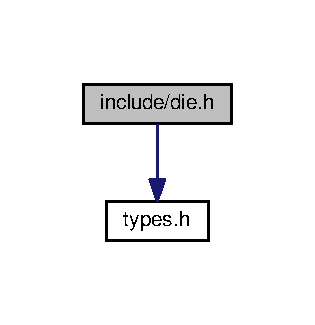
\includegraphics[width=151pt]{die_8h__incl}
\end{center}
\end{figure}
This graph shows which files directly or indirectly include this file\+:
\nopagebreak
\begin{figure}[H]
\begin{center}
\leavevmode
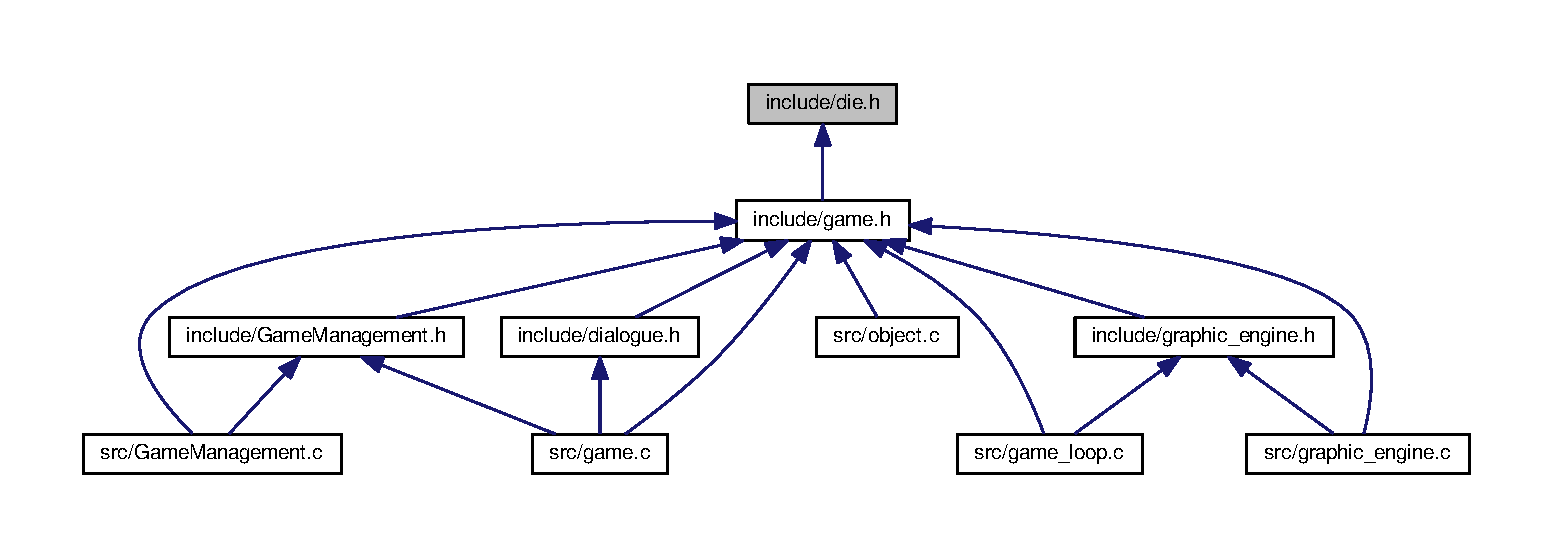
\includegraphics[width=350pt]{die_8h__dep__incl}
\end{center}
\end{figure}
\subsection*{Typedefs}
\begin{DoxyCompactItemize}
\item 
typedef struct \hyperlink{struct__Die}{\+\_\+\+Die} \hyperlink{die_8h_a892f0b0bf81d69a1f7a14ea238e36dd3}{Die}
\begin{DoxyCompactList}\small\item\em die with id and last number \end{DoxyCompactList}\end{DoxyCompactItemize}
\subsection*{Functions}
\begin{DoxyCompactItemize}
\item 
\hyperlink{die_8h_a892f0b0bf81d69a1f7a14ea238e36dd3}{Die} $\ast$ \hyperlink{die_8h_a413bced882cd5cadbb1d8feaf367ed3f}{die\+\_\+create} (\hyperlink{types_8h_a845e604fb28f7e3d97549da3448149d3}{Id} id)
\begin{DoxyCompactList}\small\item\em creates a die \end{DoxyCompactList}\item 
void \hyperlink{die_8h_a80d368f2c29bd18044c0f38fd0817bd6}{die\+\_\+destroy} (\hyperlink{die_8h_a892f0b0bf81d69a1f7a14ea238e36dd3}{Die} $\ast$d)
\begin{DoxyCompactList}\small\item\em frees memory \end{DoxyCompactList}\item 
\hyperlink{types_8h_a845e604fb28f7e3d97549da3448149d3}{Id} \hyperlink{die_8h_a39aff188cafaf3090455610aeb712a86}{die\+\_\+get\+\_\+id} (\hyperlink{die_8h_a892f0b0bf81d69a1f7a14ea238e36dd3}{Die} $\ast$d)
\begin{DoxyCompactList}\small\item\em returns the id of a die \end{DoxyCompactList}\item 
int \hyperlink{die_8h_a8f39093739dafbc2da02203255aa8930}{die\+\_\+get\+\_\+lastroll} (\hyperlink{die_8h_a892f0b0bf81d69a1f7a14ea238e36dd3}{Die} $\ast$d)
\begin{DoxyCompactList}\small\item\em returns the last value of the die \end{DoxyCompactList}\item 
\hyperlink{types_8h_a32c27cc471df37f4fc818d65de0a56c4}{S\+T\+A\+T\+US} \hyperlink{die_8h_adedf377ce1667f5506b0ee1aff756852}{die\+\_\+roll} (\hyperlink{die_8h_a892f0b0bf81d69a1f7a14ea238e36dd3}{Die} $\ast$d)
\begin{DoxyCompactList}\small\item\em generates a number between 1 and 6 \end{DoxyCompactList}\item 
void \hyperlink{die_8h_a6fffbb733d4e104d0bc4e64f13c78e9d}{die\+\_\+print\+\_\+content} (\hyperlink{die_8h_a892f0b0bf81d69a1f7a14ea238e36dd3}{Die} $\ast$d)
\begin{DoxyCompactList}\small\item\em prints the id and last roll of a die \end{DoxyCompactList}\end{DoxyCompactItemize}


\subsection{Detailed Description}
generates a die 

This module creates a dice that will generate a random number between 1 and 6 that will be the number of spaces that an object should move.

\begin{DoxyAuthor}{Author}
Juan Moreno 
\end{DoxyAuthor}
\begin{DoxyVersion}{Version}
2.\+0 
\end{DoxyVersion}
\begin{DoxyDate}{Date}
07-\/04-\/2018 
\end{DoxyDate}


\subsection{Typedef Documentation}
\index{die.\+h@{die.\+h}!Die@{Die}}
\index{Die@{Die}!die.\+h@{die.\+h}}
\subsubsection[{\texorpdfstring{Die}{Die}}]{\setlength{\rightskip}{0pt plus 5cm}typedef struct {\bf \+\_\+\+Die} {\bf Die}}\hypertarget{die_8h_a892f0b0bf81d69a1f7a14ea238e36dd3}{}\label{die_8h_a892f0b0bf81d69a1f7a14ea238e36dd3}


die with id and last number 

Struct for storing a die that will show a random number and get the last roll. 

\subsection{Function Documentation}
\index{die.\+h@{die.\+h}!die\+\_\+create@{die\+\_\+create}}
\index{die\+\_\+create@{die\+\_\+create}!die.\+h@{die.\+h}}
\subsubsection[{\texorpdfstring{die\+\_\+create(\+Id id)}{die_create(Id id)}}]{\setlength{\rightskip}{0pt plus 5cm}{\bf Die}$\ast$ die\+\_\+create (
\begin{DoxyParamCaption}
\item[{{\bf Id}}]{id}
\end{DoxyParamCaption}
)}\hypertarget{die_8h_a413bced882cd5cadbb1d8feaf367ed3f}{}\label{die_8h_a413bced882cd5cadbb1d8feaf367ed3f}


creates a die 

It creates a new inventory by initializing the variables of the structure and allocating mamory for a new die.

\begin{DoxyAuthor}{Author}
Juan Moreno 
\end{DoxyAuthor}

\begin{DoxyParams}{Parameters}
{\em id} & long int. \\
\hline
\end{DoxyParams}
\begin{DoxyReturn}{Returns}
pointer to die. 
\end{DoxyReturn}
\index{die.\+h@{die.\+h}!die\+\_\+destroy@{die\+\_\+destroy}}
\index{die\+\_\+destroy@{die\+\_\+destroy}!die.\+h@{die.\+h}}
\subsubsection[{\texorpdfstring{die\+\_\+destroy(\+Die $\ast$d)}{die_destroy(Die *d)}}]{\setlength{\rightskip}{0pt plus 5cm}void die\+\_\+destroy (
\begin{DoxyParamCaption}
\item[{{\bf Die} $\ast$}]{d}
\end{DoxyParamCaption}
)}\hypertarget{die_8h_a80d368f2c29bd18044c0f38fd0817bd6}{}\label{die_8h_a80d368f2c29bd18044c0f38fd0817bd6}


frees memory 

Receives pointer to die and frees the memory it occupied.

\begin{DoxyAuthor}{Author}
Juan Moreno 
\end{DoxyAuthor}

\begin{DoxyParams}{Parameters}
{\em d} & pointer to die. \\
\hline
\end{DoxyParams}
\begin{DoxyReturn}{Returns}
V\+O\+ID F\+U\+N\+C\+T\+I\+ON, F\+R\+E\+ES M\+E\+M\+O\+RY O\+N\+LY. 
\end{DoxyReturn}
\index{die.\+h@{die.\+h}!die\+\_\+get\+\_\+id@{die\+\_\+get\+\_\+id}}
\index{die\+\_\+get\+\_\+id@{die\+\_\+get\+\_\+id}!die.\+h@{die.\+h}}
\subsubsection[{\texorpdfstring{die\+\_\+get\+\_\+id(\+Die $\ast$d)}{die_get_id(Die *d)}}]{\setlength{\rightskip}{0pt plus 5cm}{\bf Id} die\+\_\+get\+\_\+id (
\begin{DoxyParamCaption}
\item[{{\bf Die} $\ast$}]{d}
\end{DoxyParamCaption}
)}\hypertarget{die_8h_a39aff188cafaf3090455610aeb712a86}{}\label{die_8h_a39aff188cafaf3090455610aeb712a86}


returns the id of a die 

Function in charge of returning the id of a die already created.

\begin{DoxyAuthor}{Author}
Juan Moreno 
\end{DoxyAuthor}

\begin{DoxyParams}{Parameters}
{\em d} & pointer to die. \\
\hline
\end{DoxyParams}
\begin{DoxyReturn}{Returns}
pointer to die(id of the die). 
\end{DoxyReturn}
\index{die.\+h@{die.\+h}!die\+\_\+get\+\_\+lastroll@{die\+\_\+get\+\_\+lastroll}}
\index{die\+\_\+get\+\_\+lastroll@{die\+\_\+get\+\_\+lastroll}!die.\+h@{die.\+h}}
\subsubsection[{\texorpdfstring{die\+\_\+get\+\_\+lastroll(\+Die $\ast$d)}{die_get_lastroll(Die *d)}}]{\setlength{\rightskip}{0pt plus 5cm}int die\+\_\+get\+\_\+lastroll (
\begin{DoxyParamCaption}
\item[{{\bf Die} $\ast$}]{d}
\end{DoxyParamCaption}
)}\hypertarget{die_8h_a8f39093739dafbc2da02203255aa8930}{}\label{die_8h_a8f39093739dafbc2da02203255aa8930}


returns the last value of the die 

Function in charge of returning the last roll generated by the die in orther to keep that value.

\begin{DoxyAuthor}{Author}
Juan Moreno 
\end{DoxyAuthor}

\begin{DoxyParams}{Parameters}
{\em d} & pointer to die. \\
\hline
\end{DoxyParams}
\begin{DoxyReturn}{Returns}
Number that the die rolled last time. 
\end{DoxyReturn}
\index{die.\+h@{die.\+h}!die\+\_\+print\+\_\+content@{die\+\_\+print\+\_\+content}}
\index{die\+\_\+print\+\_\+content@{die\+\_\+print\+\_\+content}!die.\+h@{die.\+h}}
\subsubsection[{\texorpdfstring{die\+\_\+print\+\_\+content(\+Die $\ast$d)}{die_print_content(Die *d)}}]{\setlength{\rightskip}{0pt plus 5cm}void die\+\_\+print\+\_\+content (
\begin{DoxyParamCaption}
\item[{{\bf Die} $\ast$}]{d}
\end{DoxyParamCaption}
)}\hypertarget{die_8h_a6fffbb733d4e104d0bc4e64f13c78e9d}{}\label{die_8h_a6fffbb733d4e104d0bc4e64f13c78e9d}


prints the id and last roll of a die 

Function in charge of printing the last roll of a die and its id in order to check that it is working correctly.

\begin{DoxyAuthor}{Author}
Juan Moreno 
\end{DoxyAuthor}

\begin{DoxyParams}{Parameters}
{\em d} & pointer to die. \\
\hline
\end{DoxyParams}
\begin{DoxyReturn}{Returns}
V\+O\+ID F\+U\+N\+C\+T\+I\+ON, O\+N\+LY P\+R\+I\+N\+TS ID A\+ND N\+U\+M\+B\+ER OF T\+HE D\+IE BY C\+A\+L\+L\+I\+NG die\+\_\+get\+\_\+lastroll. 
\end{DoxyReturn}
\index{die.\+h@{die.\+h}!die\+\_\+roll@{die\+\_\+roll}}
\index{die\+\_\+roll@{die\+\_\+roll}!die.\+h@{die.\+h}}
\subsubsection[{\texorpdfstring{die\+\_\+roll(\+Die $\ast$d)}{die_roll(Die *d)}}]{\setlength{\rightskip}{0pt plus 5cm}{\bf S\+T\+A\+T\+US} die\+\_\+roll (
\begin{DoxyParamCaption}
\item[{{\bf Die} $\ast$}]{d}
\end{DoxyParamCaption}
)}\hypertarget{die_8h_adedf377ce1667f5506b0ee1aff756852}{}\label{die_8h_adedf377ce1667f5506b0ee1aff756852}


generates a number between 1 and 6 

Rolls a die, giving a random number between 1 and 6 and storing it in lastroll.

\begin{DoxyAuthor}{Author}
Juan Moreno 
\end{DoxyAuthor}

\begin{DoxyParams}{Parameters}
{\em d} & pointer to die. \\
\hline
\end{DoxyParams}
\begin{DoxyReturn}{Returns}
S\+T\+A\+T\+US, E\+R\+R\+OR if argument received is N\+U\+LL, if not, OK. 
\end{DoxyReturn}

\hypertarget{game_8h}{}\section{include/game.h File Reference}
\label{game_8h}\index{include/game.\+h@{include/game.\+h}}


It implements the G\+A\+ME structure declarates all public \hyperlink{game_8c}{game.\+c} functions.  


{\ttfamily \#include \char`\"{}command.\+h\char`\"{}}\\*
{\ttfamily \#include \char`\"{}space.\+h\char`\"{}}\\*
{\ttfamily \#include \char`\"{}object.\+h\char`\"{}}\\*
{\ttfamily \#include \char`\"{}player.\+h\char`\"{}}\\*
{\ttfamily \#include \char`\"{}die.\+h\char`\"{}}\\*
{\ttfamily \#include \char`\"{}link.\+h\char`\"{}}\\*
Include dependency graph for game.\+h\+:
\nopagebreak
\begin{figure}[H]
\begin{center}
\leavevmode
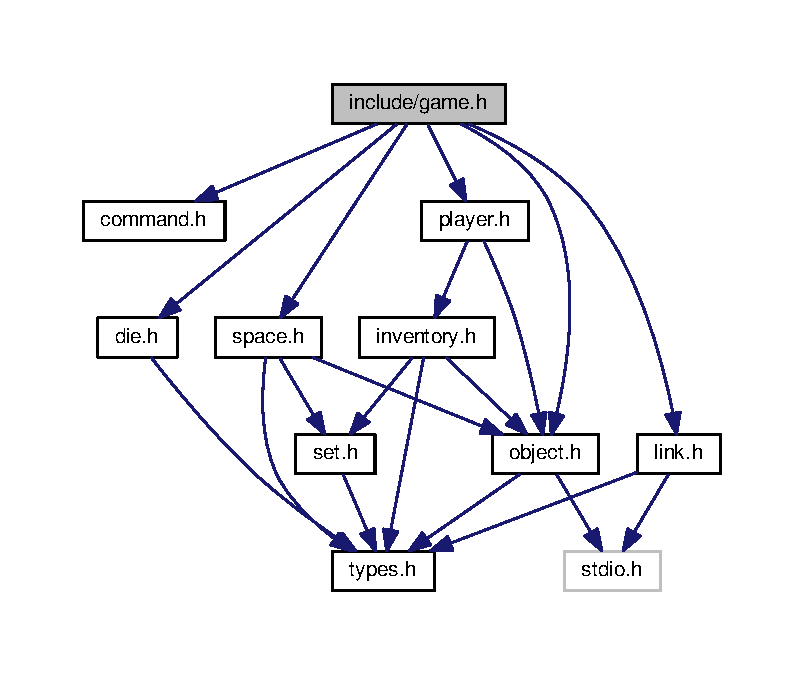
\includegraphics[width=350pt]{game_8h__incl}
\end{center}
\end{figure}
This graph shows which files directly or indirectly include this file\+:
\nopagebreak
\begin{figure}[H]
\begin{center}
\leavevmode
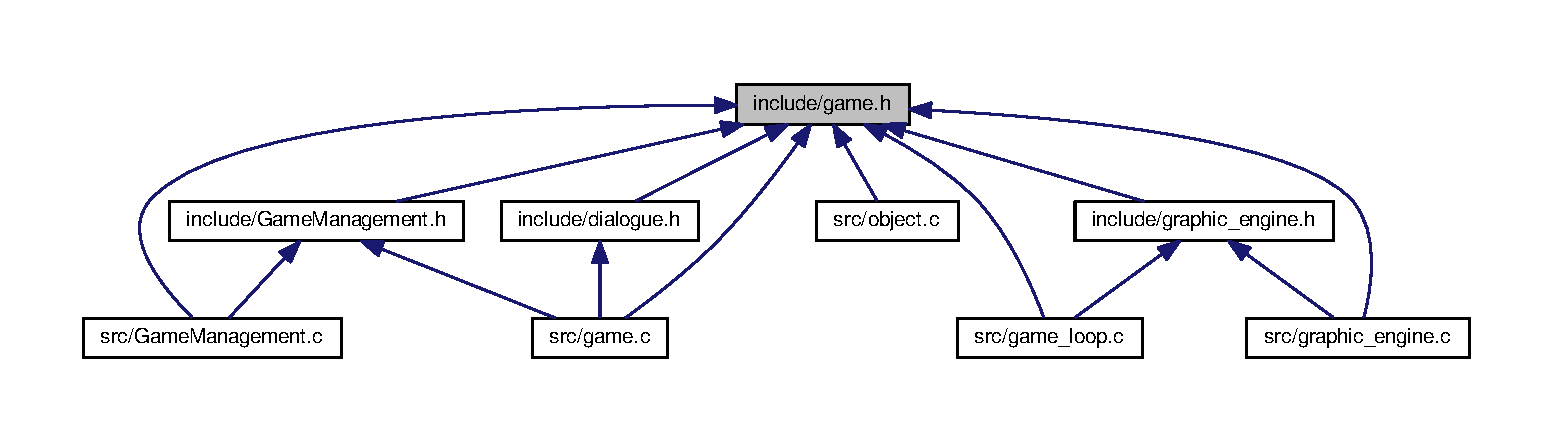
\includegraphics[width=350pt]{game_8h__dep__incl}
\end{center}
\end{figure}
\subsection*{Macros}
\begin{DoxyCompactItemize}
\item 
\#define \hyperlink{game_8h_a8e497c59a3362df6102c893a8498acd0}{M\+A\+X\+\_\+\+O\+BJ}~20
\item 
\#define \hyperlink{game_8h_a660ed1ec8604982002a0d6eced0e0367}{M\+A\+X\+\_\+\+L\+I\+N\+KS}~64
\end{DoxyCompactItemize}
\subsection*{Typedefs}
\begin{DoxyCompactItemize}
\item 
typedef struct \hyperlink{struct__Game}{\+\_\+\+Game} \hyperlink{game_8h_a57156d39c530aec3fba3a9dad8c2dc6a}{Game}
\begin{DoxyCompactList}\small\item\em game definition \end{DoxyCompactList}\end{DoxyCompactItemize}
\subsection*{Functions}
\begin{DoxyCompactItemize}
\item 
\hyperlink{game_8h_a57156d39c530aec3fba3a9dad8c2dc6a}{Game} $\ast$ \hyperlink{game_8h_a1cdbe3f06b9bf49eb5e334a22ad3b2b9}{game\+\_\+create} ()
\begin{DoxyCompactList}\small\item\em creates a game \end{DoxyCompactList}\item 
\hyperlink{types_8h_a32c27cc471df37f4fc818d65de0a56c4}{S\+T\+A\+T\+US} \hyperlink{game_8h_ae5ad86de0a92d9eccb234948458da7f1}{game\+\_\+add\+\_\+space} (\hyperlink{game_8h_a57156d39c530aec3fba3a9dad8c2dc6a}{Game} $\ast$game, \hyperlink{space_8h_a67533ffc2b70463baecc38fb0629bbfc}{Space} $\ast$space)
\begin{DoxyCompactList}\small\item\em adds a space to the game \end{DoxyCompactList}\item 
\hyperlink{types_8h_a32c27cc471df37f4fc818d65de0a56c4}{S\+T\+A\+T\+US} \hyperlink{game_8h_a9597a8e456aa74db536e87d56f56c3b4}{game\+\_\+add\+\_\+object} (\hyperlink{game_8h_a57156d39c530aec3fba3a9dad8c2dc6a}{Game} $\ast$game, \hyperlink{object_8h_a7f8bbcda919b65ce67f92fba08e0212f}{Object} $\ast$object)
\begin{DoxyCompactList}\small\item\em adds an object to the game \end{DoxyCompactList}\item 
\hyperlink{types_8h_a32c27cc471df37f4fc818d65de0a56c4}{S\+T\+A\+T\+US} \hyperlink{game_8h_afc77f90739be0fd45b7f5616e543bfae}{game\+\_\+create\+\_\+from\+\_\+file} (\hyperlink{game_8h_a57156d39c530aec3fba3a9dad8c2dc6a}{Game} $\ast$game, char $\ast$filename)
\begin{DoxyCompactList}\small\item\em calls the game\+\_\+reader functions \end{DoxyCompactList}\item 
\hyperlink{types_8h_a32c27cc471df37f4fc818d65de0a56c4}{S\+T\+A\+T\+US} \hyperlink{game_8h_a005b4f436300333e7fff8fba2027337e}{game\+\_\+update} (\hyperlink{game_8h_a57156d39c530aec3fba3a9dad8c2dc6a}{Game} $\ast$game, \hyperlink{command_8h_a0473597db8c45c0289b6b8e2f8abbe32}{T\+\_\+\+Command} cmd)
\begin{DoxyCompactList}\small\item\em executes commands \end{DoxyCompactList}\item 
\hyperlink{types_8h_a32c27cc471df37f4fc818d65de0a56c4}{S\+T\+A\+T\+US} \hyperlink{game_8h_a0736924a1235c0e6fe9b6d91c2a12af8}{game\+\_\+destroy} (\hyperlink{game_8h_a57156d39c530aec3fba3a9dad8c2dc6a}{Game} $\ast$game)
\begin{DoxyCompactList}\small\item\em Frees the memory of all the elements in a game. \end{DoxyCompactList}\item 
\hyperlink{types_8h_a3e5b8192e7d9ffaf3542f1210aec18dd}{B\+O\+OL} \hyperlink{game_8h_aa6efe0650af110bbd84e742cc8046d93}{game\+\_\+is\+\_\+over} (\hyperlink{game_8h_a57156d39c530aec3fba3a9dad8c2dc6a}{Game} $\ast$game)
\begin{DoxyCompactList}\small\item\em Checks if the game has ended. \end{DoxyCompactList}\item 
void \hyperlink{game_8h_a108f413649a6dc99d3ffeed092dc15f5}{game\+\_\+print\+\_\+screen} (\hyperlink{game_8h_a57156d39c530aec3fba3a9dad8c2dc6a}{Game} $\ast$game)
\begin{DoxyCompactList}\small\item\em prints the screen of the game \end{DoxyCompactList}\item 
void \hyperlink{game_8h_a33a5ed8937423f8c012df3cedad4fa4c}{game\+\_\+print\+\_\+data} (\hyperlink{game_8h_a57156d39c530aec3fba3a9dad8c2dc6a}{Game} $\ast$game)
\begin{DoxyCompactList}\small\item\em prints the data of the game \end{DoxyCompactList}\item 
\hyperlink{space_8h_a67533ffc2b70463baecc38fb0629bbfc}{Space} $\ast$ \hyperlink{game_8h_a69d94da9d27b542d3ebdeb8b60f1f2dc}{game\+\_\+get\+\_\+space} (\hyperlink{game_8h_a57156d39c530aec3fba3a9dad8c2dc6a}{Game} $\ast$game, \hyperlink{types_8h_a845e604fb28f7e3d97549da3448149d3}{Id} id)
\begin{DoxyCompactList}\small\item\em gets the spaces of the game \end{DoxyCompactList}\item 
\hyperlink{types_8h_a845e604fb28f7e3d97549da3448149d3}{Id} \hyperlink{game_8h_ac6a628f2106f81c37d0e83c67920615f}{game\+\_\+get\+\_\+player\+\_\+location} (\hyperlink{game_8h_a57156d39c530aec3fba3a9dad8c2dc6a}{Game} $\ast$game)
\begin{DoxyCompactList}\small\item\em gets the location of the player \end{DoxyCompactList}\item 
\hyperlink{types_8h_a845e604fb28f7e3d97549da3448149d3}{Id} \hyperlink{game_8h_a7825a43a120a5240133cd4c09f5364e1}{game\+\_\+get\+\_\+object\+\_\+location} (\hyperlink{object_8h_a7f8bbcda919b65ce67f92fba08e0212f}{Object} $\ast$object)
\begin{DoxyCompactList}\small\item\em gets the location of an object \end{DoxyCompactList}\item 
int \hyperlink{game_8h_a8726102792afb740eb8e654d933b1cc1}{game\+\_\+get\+\_\+die\+\_\+lastroll} (\hyperlink{game_8h_a57156d39c530aec3fba3a9dad8c2dc6a}{Game} $\ast$game)
\begin{DoxyCompactList}\small\item\em gets the last value of the die \end{DoxyCompactList}\item 
\hyperlink{types_8h_a32c27cc471df37f4fc818d65de0a56c4}{S\+T\+A\+T\+US} \hyperlink{game_8h_abb8b884baa9dc2d492f60210e827f5dd}{game\+\_\+get\+\_\+last\+\_\+command\+\_\+status} (\hyperlink{game_8h_a57156d39c530aec3fba3a9dad8c2dc6a}{Game} $\ast$game)
\begin{DoxyCompactList}\small\item\em gets the last command \end{DoxyCompactList}\item 
\hyperlink{types_8h_a32c27cc471df37f4fc818d65de0a56c4}{S\+T\+A\+T\+US} \hyperlink{game_8h_a7376b540583e0df561780afe83a82370}{game\+\_\+set\+\_\+object\+\_\+location} (\hyperlink{object_8h_a7f8bbcda919b65ce67f92fba08e0212f}{Object} $\ast$object, \hyperlink{types_8h_a845e604fb28f7e3d97549da3448149d3}{Id} id)
\begin{DoxyCompactList}\small\item\em sets a location for an object \end{DoxyCompactList}\item 
\hyperlink{command_8h_a0473597db8c45c0289b6b8e2f8abbe32}{T\+\_\+\+Command} \hyperlink{game_8h_ac35df1afdade2b7659ebbcfeca1f0c35}{game\+\_\+get\+\_\+last\+\_\+command} (\hyperlink{game_8h_a57156d39c530aec3fba3a9dad8c2dc6a}{Game} $\ast$game)
\begin{DoxyCompactList}\small\item\em gets the last command selected \end{DoxyCompactList}\item 
\hyperlink{object_8h_a7f8bbcda919b65ce67f92fba08e0212f}{Object} $\ast$ \hyperlink{game_8h_a286c704414005130dab85638f34ca48d}{get\+\_\+object\+\_\+from\+\_\+game} (\hyperlink{game_8h_a57156d39c530aec3fba3a9dad8c2dc6a}{Game} $\ast$game, int i)
\begin{DoxyCompactList}\small\item\em gets and object from the game \end{DoxyCompactList}\item 
char $\ast$ \hyperlink{game_8h_a0c9027fd711bd96429bee8fdfc964493}{game\+\_\+get\+\_\+aux} (\hyperlink{game_8h_a57156d39c530aec3fba3a9dad8c2dc6a}{Game} $\ast$game)
\begin{DoxyCompactList}\small\item\em gets an auxiliary string \end{DoxyCompactList}\item 
\hyperlink{types_8h_a32c27cc471df37f4fc818d65de0a56c4}{S\+T\+A\+T\+US} \hyperlink{game_8h_a4691bee17d5784ad6eb257dfbb252c27}{game\+\_\+add\+\_\+link} (\hyperlink{game_8h_a57156d39c530aec3fba3a9dad8c2dc6a}{Game} $\ast$game, \hyperlink{link_8h_ae3b299941e67be6971bfd64a25505eff}{Link} $\ast$link)
\begin{DoxyCompactList}\small\item\em adds a link to the game \end{DoxyCompactList}\item 
\hyperlink{link_8h_ae3b299941e67be6971bfd64a25505eff}{Link} $\ast$ \hyperlink{game_8h_a1064ec927b8c33cf55982b73845db7d3}{game\+\_\+get\+\_\+link} (\hyperlink{game_8h_a57156d39c530aec3fba3a9dad8c2dc6a}{Game} $\ast$game, \hyperlink{types_8h_a845e604fb28f7e3d97549da3448149d3}{Id} id)
\begin{DoxyCompactList}\small\item\em gets link of the game \end{DoxyCompactList}\item 
\hyperlink{types_8h_a32c27cc471df37f4fc818d65de0a56c4}{S\+T\+A\+T\+US} \hyperlink{game_8h_a492ca9fb594442dc43fc7d18a3820426}{game\+\_\+set\+\_\+player\+\_\+location} (\hyperlink{game_8h_a57156d39c530aec3fba3a9dad8c2dc6a}{Game} $\ast$game, \hyperlink{types_8h_a845e604fb28f7e3d97549da3448149d3}{Id} id)
\begin{DoxyCompactList}\small\item\em sets location to player \end{DoxyCompactList}\item 
\hyperlink{player_8h_af30e2030635a69690f85e48bc6ef202f}{Player} $\ast$ \hyperlink{game_8h_a7ea36d7b226f6ff5196214524b296557}{get\+\_\+player\+\_\+from\+\_\+game} (\hyperlink{game_8h_a57156d39c530aec3fba3a9dad8c2dc6a}{Game} $\ast$game)
\begin{DoxyCompactList}\small\item\em gets the player \end{DoxyCompactList}\item 
\hyperlink{die_8h_a892f0b0bf81d69a1f7a14ea238e36dd3}{Die} $\ast$ \hyperlink{game_8h_acfa528e54998d1b0e522d20b59c548e5}{get\+\_\+die\+\_\+from\+\_\+game} (\hyperlink{game_8h_a57156d39c530aec3fba3a9dad8c2dc6a}{Game} $\ast$game)
\begin{DoxyCompactList}\small\item\em gets die of the game \end{DoxyCompactList}\item 
\hyperlink{types_8h_a845e604fb28f7e3d97549da3448149d3}{Id} \hyperlink{game_8h_ad2dfd865e2bd2c545a15d33f4d1cf3ae}{game\+\_\+get\+\_\+space\+\_\+id\+\_\+at} (\hyperlink{game_8h_a57156d39c530aec3fba3a9dad8c2dc6a}{Game} $\ast$game, int position)
\begin{DoxyCompactList}\small\item\em gets the location of an space \end{DoxyCompactList}\end{DoxyCompactItemize}


\subsection{Detailed Description}
It implements the G\+A\+ME structure declarates all public \hyperlink{game_8c}{game.\+c} functions. 

\begin{DoxyAuthor}{Author}
Juan Moreno 
\end{DoxyAuthor}
\begin{DoxyVersion}{Version}
2.\+1 
\end{DoxyVersion}
\begin{DoxyDate}{Date}
07-\/04-\/2018 
\end{DoxyDate}


\subsection{Macro Definition Documentation}
\index{game.\+h@{game.\+h}!M\+A\+X\+\_\+\+L\+I\+N\+KS@{M\+A\+X\+\_\+\+L\+I\+N\+KS}}
\index{M\+A\+X\+\_\+\+L\+I\+N\+KS@{M\+A\+X\+\_\+\+L\+I\+N\+KS}!game.\+h@{game.\+h}}
\subsubsection[{\texorpdfstring{M\+A\+X\+\_\+\+L\+I\+N\+KS}{MAX_LINKS}}]{\setlength{\rightskip}{0pt plus 5cm}\#define M\+A\+X\+\_\+\+L\+I\+N\+KS~64}\hypertarget{game_8h_a660ed1ec8604982002a0d6eced0e0367}{}\label{game_8h_a660ed1ec8604982002a0d6eced0e0367}
Maximum number of links \index{game.\+h@{game.\+h}!M\+A\+X\+\_\+\+O\+BJ@{M\+A\+X\+\_\+\+O\+BJ}}
\index{M\+A\+X\+\_\+\+O\+BJ@{M\+A\+X\+\_\+\+O\+BJ}!game.\+h@{game.\+h}}
\subsubsection[{\texorpdfstring{M\+A\+X\+\_\+\+O\+BJ}{MAX_OBJ}}]{\setlength{\rightskip}{0pt plus 5cm}\#define M\+A\+X\+\_\+\+O\+BJ~20}\hypertarget{game_8h_a8e497c59a3362df6102c893a8498acd0}{}\label{game_8h_a8e497c59a3362df6102c893a8498acd0}
Maximum number of objects 

\subsection{Typedef Documentation}
\index{game.\+h@{game.\+h}!Game@{Game}}
\index{Game@{Game}!game.\+h@{game.\+h}}
\subsubsection[{\texorpdfstring{Game}{Game}}]{\setlength{\rightskip}{0pt plus 5cm}typedef struct {\bf \+\_\+\+Game} {\bf Game}}\hypertarget{game_8h_a57156d39c530aec3fba3a9dad8c2dc6a}{}\label{game_8h_a57156d39c530aec3fba3a9dad8c2dc6a}


game definition 

The game structure has everything our game needs for working excepting the graphics Privacy\+: public structure Struct for storing the elements of the game. 

\subsection{Function Documentation}
\index{game.\+h@{game.\+h}!game\+\_\+add\+\_\+link@{game\+\_\+add\+\_\+link}}
\index{game\+\_\+add\+\_\+link@{game\+\_\+add\+\_\+link}!game.\+h@{game.\+h}}
\subsubsection[{\texorpdfstring{game\+\_\+add\+\_\+link(\+Game $\ast$game, Link $\ast$link)}{game_add_link(Game *game, Link *link)}}]{\setlength{\rightskip}{0pt plus 5cm}{\bf S\+T\+A\+T\+US} game\+\_\+add\+\_\+link (
\begin{DoxyParamCaption}
\item[{{\bf Game} $\ast$}]{game, }
\item[{{\bf Link} $\ast$}]{link}
\end{DoxyParamCaption}
)}\hypertarget{game_8h_a4691bee17d5784ad6eb257dfbb252c27}{}\label{game_8h_a4691bee17d5784ad6eb257dfbb252c27}


adds a link to the game 

It is the function in charge of adding links to the game when considering it appropriate.

\begin{DoxyAuthor}{Author}
Juan Moreno 
\end{DoxyAuthor}

\begin{DoxyParams}{Parameters}
{\em game} & pointer to game. \\
\hline
{\em link} & pointer to link \\
\hline
\end{DoxyParams}
\begin{DoxyReturn}{Returns}
S\+T\+A\+T\+US, E\+R\+R\+OR if argument received is N\+U\+LL, if not, OK. 
\end{DoxyReturn}
\index{game.\+h@{game.\+h}!game\+\_\+add\+\_\+object@{game\+\_\+add\+\_\+object}}
\index{game\+\_\+add\+\_\+object@{game\+\_\+add\+\_\+object}!game.\+h@{game.\+h}}
\subsubsection[{\texorpdfstring{game\+\_\+add\+\_\+object(\+Game $\ast$game, Object $\ast$object)}{game_add_object(Game *game, Object *object)}}]{\setlength{\rightskip}{0pt plus 5cm}{\bf S\+T\+A\+T\+US} game\+\_\+add\+\_\+object (
\begin{DoxyParamCaption}
\item[{{\bf Game} $\ast$}]{game, }
\item[{{\bf Object} $\ast$}]{object}
\end{DoxyParamCaption}
)}\hypertarget{game_8h_a9597a8e456aa74db536e87d56f56c3b4}{}\label{game_8h_a9597a8e456aa74db536e87d56f56c3b4}


adds an object to the game 

\begin{DoxyAuthor}{Author}
Juan Moreno 
\end{DoxyAuthor}

\begin{DoxyParams}{Parameters}
{\em game} & pointer to game. \\
\hline
{\em object} & pointer to object. \\
\hline
\end{DoxyParams}
\begin{DoxyReturn}{Returns}
S\+T\+A\+T\+US, E\+R\+R\+OR if argument received is N\+U\+LL, if not, OK. 
\end{DoxyReturn}
\index{game.\+h@{game.\+h}!game\+\_\+add\+\_\+space@{game\+\_\+add\+\_\+space}}
\index{game\+\_\+add\+\_\+space@{game\+\_\+add\+\_\+space}!game.\+h@{game.\+h}}
\subsubsection[{\texorpdfstring{game\+\_\+add\+\_\+space(\+Game $\ast$game, Space $\ast$space)}{game_add_space(Game *game, Space *space)}}]{\setlength{\rightskip}{0pt plus 5cm}{\bf S\+T\+A\+T\+US} game\+\_\+add\+\_\+space (
\begin{DoxyParamCaption}
\item[{{\bf Game} $\ast$}]{game, }
\item[{{\bf Space} $\ast$}]{space}
\end{DoxyParamCaption}
)}\hypertarget{game_8h_ae5ad86de0a92d9eccb234948458da7f1}{}\label{game_8h_ae5ad86de0a92d9eccb234948458da7f1}


adds a space to the game 

\begin{DoxyAuthor}{Author}
Juan Moreno 
\end{DoxyAuthor}

\begin{DoxyParams}{Parameters}
{\em game} & pointer to game. \\
\hline
{\em space} & pointer to space. \\
\hline
\end{DoxyParams}
\begin{DoxyReturn}{Returns}
S\+T\+A\+T\+US, E\+R\+R\+OR if argument received is N\+U\+LL, if not, OK.
\end{DoxyReturn}
adds a space to the game

Private functions Function that implements spaces by using the set module to add values.

\begin{DoxyAuthor}{Author}
Juan Moreno 
\end{DoxyAuthor}

\begin{DoxyParams}{Parameters}
{\em game} & pointer to game. \\
\hline
{\em space} & pointer to space. \\
\hline
\end{DoxyParams}
\begin{DoxyReturn}{Returns}
S\+T\+A\+T\+US, E\+R\+R\+OR if argument received is N\+U\+LL, if not, OK. 
\end{DoxyReturn}
\index{game.\+h@{game.\+h}!game\+\_\+create@{game\+\_\+create}}
\index{game\+\_\+create@{game\+\_\+create}!game.\+h@{game.\+h}}
\subsubsection[{\texorpdfstring{game\+\_\+create()}{game_create()}}]{\setlength{\rightskip}{0pt plus 5cm}{\bf Game}$\ast$ game\+\_\+create (
\begin{DoxyParamCaption}
{}
\end{DoxyParamCaption}
)}\hypertarget{game_8h_a1cdbe3f06b9bf49eb5e334a22ad3b2b9}{}\label{game_8h_a1cdbe3f06b9bf49eb5e334a22ad3b2b9}


creates a game 

Creates a new game, allocating memory for its spaces and for the structure game itself and initializating to null other. It also creates a die.

\begin{DoxyAuthor}{Author}
Juan Moreno 
\end{DoxyAuthor}
\begin{DoxyReturn}{Returns}
Pointer to game if everything wen correctly, N\+U\+LL in other case
\end{DoxyReturn}
Game interface implementation \index{game.\+h@{game.\+h}!game\+\_\+create\+\_\+from\+\_\+file@{game\+\_\+create\+\_\+from\+\_\+file}}
\index{game\+\_\+create\+\_\+from\+\_\+file@{game\+\_\+create\+\_\+from\+\_\+file}!game.\+h@{game.\+h}}
\subsubsection[{\texorpdfstring{game\+\_\+create\+\_\+from\+\_\+file(\+Game $\ast$game, char $\ast$filename)}{game_create_from_file(Game *game, char *filename)}}]{\setlength{\rightskip}{0pt plus 5cm}{\bf S\+T\+A\+T\+US} game\+\_\+create\+\_\+from\+\_\+file (
\begin{DoxyParamCaption}
\item[{{\bf Game} $\ast$}]{game, }
\item[{char $\ast$}]{filename}
\end{DoxyParamCaption}
)}\hypertarget{game_8h_afc77f90739be0fd45b7f5616e543bfae}{}\label{game_8h_afc77f90739be0fd45b7f5616e543bfae}


calls the game\+\_\+reader functions 

Calls to game create to create a new game and calls the game\+\_\+reader functions to load the game\textquotesingle{}s content from the file.

\begin{DoxyAuthor}{Author}
Juan Moreno 
\end{DoxyAuthor}

\begin{DoxyParams}{Parameters}
{\em game} & pointer to game. \\
\hline
{\em filename} & a string containing the name of the file to open. \\
\hline
\end{DoxyParams}
\begin{DoxyReturn}{Returns}
S\+T\+A\+T\+US, E\+R\+R\+OR if argument received is N\+U\+LL, if not, OK. 
\end{DoxyReturn}
\index{game.\+h@{game.\+h}!game\+\_\+destroy@{game\+\_\+destroy}}
\index{game\+\_\+destroy@{game\+\_\+destroy}!game.\+h@{game.\+h}}
\subsubsection[{\texorpdfstring{game\+\_\+destroy(\+Game $\ast$game)}{game_destroy(Game *game)}}]{\setlength{\rightskip}{0pt plus 5cm}{\bf S\+T\+A\+T\+US} game\+\_\+destroy (
\begin{DoxyParamCaption}
\item[{{\bf Game} $\ast$}]{game}
\end{DoxyParamCaption}
)}\hypertarget{game_8h_a0736924a1235c0e6fe9b6d91c2a12af8}{}\label{game_8h_a0736924a1235c0e6fe9b6d91c2a12af8}


Frees the memory of all the elements in a game. 

Receives pointer to game and frees the memory it occupied.

\begin{DoxyAuthor}{Author}
Juan Moreno 
\end{DoxyAuthor}

\begin{DoxyParams}{Parameters}
{\em game} & pointer to game. \\
\hline
\end{DoxyParams}
\begin{DoxyReturn}{Returns}
S\+T\+A\+T\+US, E\+R\+R\+OR if argument received is N\+U\+LL, if not, OK. 
\end{DoxyReturn}
\index{game.\+h@{game.\+h}!game\+\_\+get\+\_\+aux@{game\+\_\+get\+\_\+aux}}
\index{game\+\_\+get\+\_\+aux@{game\+\_\+get\+\_\+aux}!game.\+h@{game.\+h}}
\subsubsection[{\texorpdfstring{game\+\_\+get\+\_\+aux(\+Game $\ast$game)}{game_get_aux(Game *game)}}]{\setlength{\rightskip}{0pt plus 5cm}char$\ast$ game\+\_\+get\+\_\+aux (
\begin{DoxyParamCaption}
\item[{{\bf Game} $\ast$}]{game}
\end{DoxyParamCaption}
)}\hypertarget{game_8h_a0c9027fd711bd96429bee8fdfc964493}{}\label{game_8h_a0c9027fd711bd96429bee8fdfc964493}


gets an auxiliary string 

Function that returns a string that enables the writing

\begin{DoxyAuthor}{Author}
Juan Moreno 
\end{DoxyAuthor}

\begin{DoxyParams}{Parameters}
{\em game} & pointer to game. \\
\hline
\end{DoxyParams}
\begin{DoxyReturn}{Returns}
pointer to game (char string). 
\end{DoxyReturn}
\index{game.\+h@{game.\+h}!game\+\_\+get\+\_\+die\+\_\+lastroll@{game\+\_\+get\+\_\+die\+\_\+lastroll}}
\index{game\+\_\+get\+\_\+die\+\_\+lastroll@{game\+\_\+get\+\_\+die\+\_\+lastroll}!game.\+h@{game.\+h}}
\subsubsection[{\texorpdfstring{game\+\_\+get\+\_\+die\+\_\+lastroll(\+Game $\ast$game)}{game_get_die_lastroll(Game *game)}}]{\setlength{\rightskip}{0pt plus 5cm}int game\+\_\+get\+\_\+die\+\_\+lastroll (
\begin{DoxyParamCaption}
\item[{{\bf Game} $\ast$}]{game}
\end{DoxyParamCaption}
)}\hypertarget{game_8h_a8726102792afb740eb8e654d933b1cc1}{}\label{game_8h_a8726102792afb740eb8e654d933b1cc1}


gets the last value of the die 

Returns the value of the game\textquotesingle{}s die last roll.

\begin{DoxyAuthor}{Author}
Juan Moreno 
\end{DoxyAuthor}

\begin{DoxyParams}{Parameters}
{\em game} & pointer to game. \\
\hline
\end{DoxyParams}
\begin{DoxyReturn}{Returns}
the last number generated of the die (int). 
\end{DoxyReturn}
\index{game.\+h@{game.\+h}!game\+\_\+get\+\_\+last\+\_\+command@{game\+\_\+get\+\_\+last\+\_\+command}}
\index{game\+\_\+get\+\_\+last\+\_\+command@{game\+\_\+get\+\_\+last\+\_\+command}!game.\+h@{game.\+h}}
\subsubsection[{\texorpdfstring{game\+\_\+get\+\_\+last\+\_\+command(\+Game $\ast$game)}{game_get_last_command(Game *game)}}]{\setlength{\rightskip}{0pt plus 5cm}{\bf T\+\_\+\+Command} game\+\_\+get\+\_\+last\+\_\+command (
\begin{DoxyParamCaption}
\item[{{\bf Game} $\ast$}]{game}
\end{DoxyParamCaption}
)}\hypertarget{game_8h_ac35df1afdade2b7659ebbcfeca1f0c35}{}\label{game_8h_ac35df1afdade2b7659ebbcfeca1f0c35}


gets the last command selected 

Returns the last command used by the player.

\begin{DoxyAuthor}{Author}
Juan Moreno 
\end{DoxyAuthor}

\begin{DoxyParams}{Parameters}
{\em game} & pointer to game. \\
\hline
\end{DoxyParams}
\begin{DoxyReturn}{Returns}
\hyperlink{command_8h_a0473597db8c45c0289b6b8e2f8abbe32}{T\+\_\+\+Command} ==$>$ The last command used by the player. 
\end{DoxyReturn}
\index{game.\+h@{game.\+h}!game\+\_\+get\+\_\+last\+\_\+command\+\_\+status@{game\+\_\+get\+\_\+last\+\_\+command\+\_\+status}}
\index{game\+\_\+get\+\_\+last\+\_\+command\+\_\+status@{game\+\_\+get\+\_\+last\+\_\+command\+\_\+status}!game.\+h@{game.\+h}}
\subsubsection[{\texorpdfstring{game\+\_\+get\+\_\+last\+\_\+command\+\_\+status(\+Game $\ast$game)}{game_get_last_command_status(Game *game)}}]{\setlength{\rightskip}{0pt plus 5cm}{\bf S\+T\+A\+T\+US} game\+\_\+get\+\_\+last\+\_\+command\+\_\+status (
\begin{DoxyParamCaption}
\item[{{\bf Game} $\ast$}]{game}
\end{DoxyParamCaption}
)}\hypertarget{game_8h_abb8b884baa9dc2d492f60210e827f5dd}{}\label{game_8h_abb8b884baa9dc2d492f60210e827f5dd}


gets the last command 

Returns the status of the last command used

\begin{DoxyAuthor}{Author}
Juan Moreno 
\end{DoxyAuthor}

\begin{DoxyParams}{Parameters}
{\em game} & pointer to game. \\
\hline
\end{DoxyParams}
\begin{DoxyReturn}{Returns}
S\+T\+A\+T\+US, E\+R\+R\+OR if argument received is N\+U\+LL, if not, OK. 
\end{DoxyReturn}
\index{game.\+h@{game.\+h}!game\+\_\+get\+\_\+link@{game\+\_\+get\+\_\+link}}
\index{game\+\_\+get\+\_\+link@{game\+\_\+get\+\_\+link}!game.\+h@{game.\+h}}
\subsubsection[{\texorpdfstring{game\+\_\+get\+\_\+link(\+Game $\ast$game, Id id)}{game_get_link(Game *game, Id id)}}]{\setlength{\rightskip}{0pt plus 5cm}{\bf Link}$\ast$ game\+\_\+get\+\_\+link (
\begin{DoxyParamCaption}
\item[{{\bf Game} $\ast$}]{game, }
\item[{{\bf Id}}]{id}
\end{DoxyParamCaption}
)}\hypertarget{game_8h_a1064ec927b8c33cf55982b73845db7d3}{}\label{game_8h_a1064ec927b8c33cf55982b73845db7d3}


gets link of the game 

Returns the id of a link doing it in the game module.

\begin{DoxyAuthor}{Author}
Juan Moreno 
\end{DoxyAuthor}

\begin{DoxyParams}{Parameters}
{\em game} & pointer to game. \\
\hline
{\em id} & long int. \\
\hline
\end{DoxyParams}
\begin{DoxyReturn}{Returns}
pointer to link. 
\end{DoxyReturn}
\index{game.\+h@{game.\+h}!game\+\_\+get\+\_\+object\+\_\+location@{game\+\_\+get\+\_\+object\+\_\+location}}
\index{game\+\_\+get\+\_\+object\+\_\+location@{game\+\_\+get\+\_\+object\+\_\+location}!game.\+h@{game.\+h}}
\subsubsection[{\texorpdfstring{game\+\_\+get\+\_\+object\+\_\+location(\+Object $\ast$object)}{game_get_object_location(Object *object)}}]{\setlength{\rightskip}{0pt plus 5cm}{\bf Id} game\+\_\+get\+\_\+object\+\_\+location (
\begin{DoxyParamCaption}
\item[{{\bf Object} $\ast$}]{object}
\end{DoxyParamCaption}
)}\hypertarget{game_8h_a7825a43a120a5240133cd4c09f5364e1}{}\label{game_8h_a7825a43a120a5240133cd4c09f5364e1}


gets the location of an object 

Returns the id where the object is located at that moment.

\begin{DoxyAuthor}{Author}
Juan Moreno 
\end{DoxyAuthor}

\begin{DoxyParams}{Parameters}
{\em object} & pointer to object. \\
\hline
\end{DoxyParams}
\begin{DoxyReturn}{Returns}
An id representing the player\textquotesingle{}s location. 
\end{DoxyReturn}
\index{game.\+h@{game.\+h}!game\+\_\+get\+\_\+player\+\_\+location@{game\+\_\+get\+\_\+player\+\_\+location}}
\index{game\+\_\+get\+\_\+player\+\_\+location@{game\+\_\+get\+\_\+player\+\_\+location}!game.\+h@{game.\+h}}
\subsubsection[{\texorpdfstring{game\+\_\+get\+\_\+player\+\_\+location(\+Game $\ast$game)}{game_get_player_location(Game *game)}}]{\setlength{\rightskip}{0pt plus 5cm}{\bf Id} game\+\_\+get\+\_\+player\+\_\+location (
\begin{DoxyParamCaption}
\item[{{\bf Game} $\ast$}]{game}
\end{DoxyParamCaption}
)}\hypertarget{game_8h_ac6a628f2106f81c37d0e83c67920615f}{}\label{game_8h_ac6a628f2106f81c37d0e83c67920615f}


gets the location of the player 

Returns the id where the player is located at that moment.

\begin{DoxyAuthor}{Author}
Juan Moreno 
\end{DoxyAuthor}

\begin{DoxyParams}{Parameters}
{\em game} & pointer to game \\
\hline
\end{DoxyParams}
\begin{DoxyReturn}{Returns}
An id representing the player\textquotesingle{}s location. 
\end{DoxyReturn}
\index{game.\+h@{game.\+h}!game\+\_\+get\+\_\+space@{game\+\_\+get\+\_\+space}}
\index{game\+\_\+get\+\_\+space@{game\+\_\+get\+\_\+space}!game.\+h@{game.\+h}}
\subsubsection[{\texorpdfstring{game\+\_\+get\+\_\+space(\+Game $\ast$game, Id id)}{game_get_space(Game *game, Id id)}}]{\setlength{\rightskip}{0pt plus 5cm}{\bf Space}$\ast$ game\+\_\+get\+\_\+space (
\begin{DoxyParamCaption}
\item[{{\bf Game} $\ast$}]{game, }
\item[{{\bf Id}}]{id}
\end{DoxyParamCaption}
)}\hypertarget{game_8h_a69d94da9d27b542d3ebdeb8b60f1f2dc}{}\label{game_8h_a69d94da9d27b542d3ebdeb8b60f1f2dc}


gets the spaces of the game 

Returns a pointer to a space with a determined id.

\begin{DoxyAuthor}{Author}
Juan Moreno 
\end{DoxyAuthor}

\begin{DoxyParams}{Parameters}
{\em game} & pointer to game \\
\hline
{\em id} & long int. \\
\hline
\end{DoxyParams}
\begin{DoxyReturn}{Returns}
the spaces of the game(pointer to space), N\+U\+LL if something goes wrong. 
\end{DoxyReturn}
\index{game.\+h@{game.\+h}!game\+\_\+get\+\_\+space\+\_\+id\+\_\+at@{game\+\_\+get\+\_\+space\+\_\+id\+\_\+at}}
\index{game\+\_\+get\+\_\+space\+\_\+id\+\_\+at@{game\+\_\+get\+\_\+space\+\_\+id\+\_\+at}!game.\+h@{game.\+h}}
\subsubsection[{\texorpdfstring{game\+\_\+get\+\_\+space\+\_\+id\+\_\+at(\+Game $\ast$game, int position)}{game_get_space_id_at(Game *game, int position)}}]{\setlength{\rightskip}{0pt plus 5cm}{\bf Id} game\+\_\+get\+\_\+space\+\_\+id\+\_\+at (
\begin{DoxyParamCaption}
\item[{{\bf Game} $\ast$}]{game, }
\item[{int}]{position}
\end{DoxyParamCaption}
)}\hypertarget{game_8h_ad2dfd865e2bd2c545a15d33f4d1cf3ae}{}\label{game_8h_ad2dfd865e2bd2c545a15d33f4d1cf3ae}


gets the location of an space 

Returns the id where the space is located at.

\begin{DoxyAuthor}{Author}
Juan Moreno 
\end{DoxyAuthor}

\begin{DoxyParams}{Parameters}
{\em game} & pointer to game. \\
\hline
{\em position} & int value. \\
\hline
\end{DoxyParams}
\begin{DoxyReturn}{Returns}
An id representing the space´s location.
\end{DoxyReturn}
gets the location of an space

Function in charge of returning the id of a space in the game.

\begin{DoxyAuthor}{Author}
Juan Moreno 
\end{DoxyAuthor}

\begin{DoxyParams}{Parameters}
{\em game} & pointer to game. \\
\hline
{\em position} & int. \\
\hline
\end{DoxyParams}
\begin{DoxyReturn}{Returns}
Id, N\+O\+\_\+\+ID if inventory is pointing N\+U\+LL. 
\end{DoxyReturn}
\index{game.\+h@{game.\+h}!game\+\_\+is\+\_\+over@{game\+\_\+is\+\_\+over}}
\index{game\+\_\+is\+\_\+over@{game\+\_\+is\+\_\+over}!game.\+h@{game.\+h}}
\subsubsection[{\texorpdfstring{game\+\_\+is\+\_\+over(\+Game $\ast$game)}{game_is_over(Game *game)}}]{\setlength{\rightskip}{0pt plus 5cm}{\bf B\+O\+OL} game\+\_\+is\+\_\+over (
\begin{DoxyParamCaption}
\item[{{\bf Game} $\ast$}]{game}
\end{DoxyParamCaption}
)}\hypertarget{game_8h_aa6efe0650af110bbd84e742cc8046d93}{}\label{game_8h_aa6efe0650af110bbd84e742cc8046d93}


Checks if the game has ended. 

\begin{DoxyAuthor}{Author}
Juan Moreno 
\end{DoxyAuthor}

\begin{DoxyParams}{Parameters}
{\em game} & pointer to game. \\
\hline
\end{DoxyParams}
\begin{DoxyReturn}{Returns}
B\+O\+OL, F\+A\+L\+SE if when checking is not correct, if it is correct, T\+R\+UE. 
\end{DoxyReturn}
\index{game.\+h@{game.\+h}!game\+\_\+print\+\_\+data@{game\+\_\+print\+\_\+data}}
\index{game\+\_\+print\+\_\+data@{game\+\_\+print\+\_\+data}!game.\+h@{game.\+h}}
\subsubsection[{\texorpdfstring{game\+\_\+print\+\_\+data(\+Game $\ast$game)}{game_print_data(Game *game)}}]{\setlength{\rightskip}{0pt plus 5cm}void game\+\_\+print\+\_\+data (
\begin{DoxyParamCaption}
\item[{{\bf Game} $\ast$}]{game}
\end{DoxyParamCaption}
)}\hypertarget{game_8h_a33a5ed8937423f8c012df3cedad4fa4c}{}\label{game_8h_a33a5ed8937423f8c012df3cedad4fa4c}


prints the data of the game 

If game is not pointing to N\+U\+LL, the function prints the data of the game.

\begin{DoxyAuthor}{Author}
Juan Moreno 
\end{DoxyAuthor}

\begin{DoxyParams}{Parameters}
{\em game} & pointer to game. \\
\hline
\end{DoxyParams}
\begin{DoxyReturn}{Returns}
void function. 
\end{DoxyReturn}
\index{game.\+h@{game.\+h}!game\+\_\+print\+\_\+screen@{game\+\_\+print\+\_\+screen}}
\index{game\+\_\+print\+\_\+screen@{game\+\_\+print\+\_\+screen}!game.\+h@{game.\+h}}
\subsubsection[{\texorpdfstring{game\+\_\+print\+\_\+screen(\+Game $\ast$game)}{game_print_screen(Game *game)}}]{\setlength{\rightskip}{0pt plus 5cm}void game\+\_\+print\+\_\+screen (
\begin{DoxyParamCaption}
\item[{{\bf Game} $\ast$}]{game}
\end{DoxyParamCaption}
)}\hypertarget{game_8h_a108f413649a6dc99d3ffeed092dc15f5}{}\label{game_8h_a108f413649a6dc99d3ffeed092dc15f5}


prints the screen of the game 

If game is not pointing to N\+U\+LL, the function prints the screen of the game.

\begin{DoxyAuthor}{Author}
Juan Moreno 
\end{DoxyAuthor}

\begin{DoxyParams}{Parameters}
{\em game} & pointer to game. \\
\hline
\end{DoxyParams}
\begin{DoxyReturn}{Returns}
void function. 
\end{DoxyReturn}
\index{game.\+h@{game.\+h}!game\+\_\+set\+\_\+object\+\_\+location@{game\+\_\+set\+\_\+object\+\_\+location}}
\index{game\+\_\+set\+\_\+object\+\_\+location@{game\+\_\+set\+\_\+object\+\_\+location}!game.\+h@{game.\+h}}
\subsubsection[{\texorpdfstring{game\+\_\+set\+\_\+object\+\_\+location(\+Object $\ast$object, Id id)}{game_set_object_location(Object *object, Id id)}}]{\setlength{\rightskip}{0pt plus 5cm}{\bf S\+T\+A\+T\+US} game\+\_\+set\+\_\+object\+\_\+location (
\begin{DoxyParamCaption}
\item[{{\bf Object} $\ast$}]{object, }
\item[{{\bf Id}}]{id}
\end{DoxyParamCaption}
)}\hypertarget{game_8h_a7376b540583e0df561780afe83a82370}{}\label{game_8h_a7376b540583e0df561780afe83a82370}


sets a location for an object 

Modifies the location where an object is placed.

\begin{DoxyAuthor}{Author}
Juan Moreno 
\end{DoxyAuthor}

\begin{DoxyParams}{Parameters}
{\em object} & pointer to object. \\
\hline
{\em id} & long int. \\
\hline
\end{DoxyParams}
\begin{DoxyReturn}{Returns}
S\+T\+A\+T\+US, E\+R\+R\+OR if argument received is N\+U\+LL, if not, OK. 
\end{DoxyReturn}
\index{game.\+h@{game.\+h}!game\+\_\+set\+\_\+player\+\_\+location@{game\+\_\+set\+\_\+player\+\_\+location}}
\index{game\+\_\+set\+\_\+player\+\_\+location@{game\+\_\+set\+\_\+player\+\_\+location}!game.\+h@{game.\+h}}
\subsubsection[{\texorpdfstring{game\+\_\+set\+\_\+player\+\_\+location(\+Game $\ast$game, Id id)}{game_set_player_location(Game *game, Id id)}}]{\setlength{\rightskip}{0pt plus 5cm}{\bf S\+T\+A\+T\+US} game\+\_\+set\+\_\+player\+\_\+location (
\begin{DoxyParamCaption}
\item[{{\bf Game} $\ast$}]{game, }
\item[{{\bf Id}}]{id}
\end{DoxyParamCaption}
)}\hypertarget{game_8h_a492ca9fb594442dc43fc7d18a3820426}{}\label{game_8h_a492ca9fb594442dc43fc7d18a3820426}


sets location to player 

It is the function in charge of setting a principal location(id) to the player.

\begin{DoxyAuthor}{Author}
Juan Moreno 
\end{DoxyAuthor}

\begin{DoxyParams}{Parameters}
{\em game} & pointer to game. \\
\hline
{\em id} & long int. \\
\hline
\end{DoxyParams}
\begin{DoxyReturn}{Returns}
S\+T\+A\+T\+US, E\+R\+R\+OR if argument received is N\+U\+LL, if not, OK.
\end{DoxyReturn}
sets location to player

Function in charge of setting a location for a player in the game.

\begin{DoxyAuthor}{Author}
Juan Moreno 
\end{DoxyAuthor}

\begin{DoxyParams}{Parameters}
{\em game} & pointer to game. \\
\hline
{\em id} & long int. \\
\hline
\end{DoxyParams}
\begin{DoxyReturn}{Returns}
S\+T\+A\+T\+US, E\+R\+R\+OR if argument received is N\+U\+LL, if not, OK. 
\end{DoxyReturn}
\index{game.\+h@{game.\+h}!game\+\_\+update@{game\+\_\+update}}
\index{game\+\_\+update@{game\+\_\+update}!game.\+h@{game.\+h}}
\subsubsection[{\texorpdfstring{game\+\_\+update(\+Game $\ast$game, T\+\_\+\+Command cmd)}{game_update(Game *game, T_Command cmd)}}]{\setlength{\rightskip}{0pt plus 5cm}{\bf S\+T\+A\+T\+US} game\+\_\+update (
\begin{DoxyParamCaption}
\item[{{\bf Game} $\ast$}]{game, }
\item[{{\bf T\+\_\+\+Command}}]{cmd}
\end{DoxyParamCaption}
)}\hypertarget{game_8h_a005b4f436300333e7fff8fba2027337e}{}\label{game_8h_a005b4f436300333e7fff8fba2027337e}


executes commands 

Calls a callback function executing the command defined in it.

\begin{DoxyAuthor}{Author}
Juan Moreno 
\end{DoxyAuthor}

\begin{DoxyParams}{Parameters}
{\em game} & pointer to game. \\
\hline
{\em cmd} & the command to be used. \\
\hline
\end{DoxyParams}
\begin{DoxyReturn}{Returns}
S\+T\+A\+T\+US, E\+R\+R\+OR if argument received is N\+U\+LL, if not, OK. 
\end{DoxyReturn}
\index{game.\+h@{game.\+h}!get\+\_\+die\+\_\+from\+\_\+game@{get\+\_\+die\+\_\+from\+\_\+game}}
\index{get\+\_\+die\+\_\+from\+\_\+game@{get\+\_\+die\+\_\+from\+\_\+game}!game.\+h@{game.\+h}}
\subsubsection[{\texorpdfstring{get\+\_\+die\+\_\+from\+\_\+game(\+Game $\ast$game)}{get_die_from_game(Game *game)}}]{\setlength{\rightskip}{0pt plus 5cm}{\bf Die}$\ast$ get\+\_\+die\+\_\+from\+\_\+game (
\begin{DoxyParamCaption}
\item[{{\bf Game} $\ast$}]{game}
\end{DoxyParamCaption}
)}\hypertarget{game_8h_acfa528e54998d1b0e522d20b59c548e5}{}\label{game_8h_acfa528e54998d1b0e522d20b59c548e5}


gets die of the game 

Returns the value of the die in the game.

\begin{DoxyAuthor}{Author}
Juan Moreno 
\end{DoxyAuthor}

\begin{DoxyParams}{Parameters}
{\em game} & pointer to game. \\
\hline
\end{DoxyParams}
\begin{DoxyReturn}{Returns}
pointer to die. 
\end{DoxyReturn}
\index{game.\+h@{game.\+h}!get\+\_\+object\+\_\+from\+\_\+game@{get\+\_\+object\+\_\+from\+\_\+game}}
\index{get\+\_\+object\+\_\+from\+\_\+game@{get\+\_\+object\+\_\+from\+\_\+game}!game.\+h@{game.\+h}}
\subsubsection[{\texorpdfstring{get\+\_\+object\+\_\+from\+\_\+game(\+Game $\ast$game, int i)}{get_object_from_game(Game *game, int i)}}]{\setlength{\rightskip}{0pt plus 5cm}{\bf Object}$\ast$ get\+\_\+object\+\_\+from\+\_\+game (
\begin{DoxyParamCaption}
\item[{{\bf Game} $\ast$}]{game, }
\item[{int}]{i}
\end{DoxyParamCaption}
)}\hypertarget{game_8h_a286c704414005130dab85638f34ca48d}{}\label{game_8h_a286c704414005130dab85638f34ca48d}


gets and object from the game 

Returns an object, but this time it will be defined with a pointer to game.

\begin{DoxyAuthor}{Author}
Juan Moreno 
\end{DoxyAuthor}

\begin{DoxyParams}{Parameters}
{\em game} & pointer to game. \\
\hline
{\em i} & int (i). \\
\hline
\end{DoxyParams}
\begin{DoxyReturn}{Returns}
pointer to game (object from game struct), N\+U\+LL if something goes wrong. 
\end{DoxyReturn}
\index{game.\+h@{game.\+h}!get\+\_\+player\+\_\+from\+\_\+game@{get\+\_\+player\+\_\+from\+\_\+game}}
\index{get\+\_\+player\+\_\+from\+\_\+game@{get\+\_\+player\+\_\+from\+\_\+game}!game.\+h@{game.\+h}}
\subsubsection[{\texorpdfstring{get\+\_\+player\+\_\+from\+\_\+game(\+Game $\ast$game)}{get_player_from_game(Game *game)}}]{\setlength{\rightskip}{0pt plus 5cm}{\bf Player}$\ast$ get\+\_\+player\+\_\+from\+\_\+game (
\begin{DoxyParamCaption}
\item[{{\bf Game} $\ast$}]{game}
\end{DoxyParamCaption}
)}\hypertarget{game_8h_a7ea36d7b226f6ff5196214524b296557}{}\label{game_8h_a7ea36d7b226f6ff5196214524b296557}


gets the player 

Function in charge of returning the actual player that is playing the game.

\begin{DoxyAuthor}{Author}
Juan Moreno 
\end{DoxyAuthor}

\begin{DoxyParams}{Parameters}
{\em game} & pointer to game. \\
\hline
\end{DoxyParams}
\begin{DoxyReturn}{Returns}
pointer to player. 
\end{DoxyReturn}

\hypertarget{GameManagement_8h}{}\section{include/\+Game\+Management.h File Reference}
\label{GameManagement_8h}\index{include/\+Game\+Management.\+h@{include/\+Game\+Management.\+h}}


Contains the declaration for game\+\_\+reader.\+c functions.  


{\ttfamily \#include \char`\"{}game.\+h\char`\"{}}\\*
Include dependency graph for Game\+Management.\+h\+:
\nopagebreak
\begin{figure}[H]
\begin{center}
\leavevmode
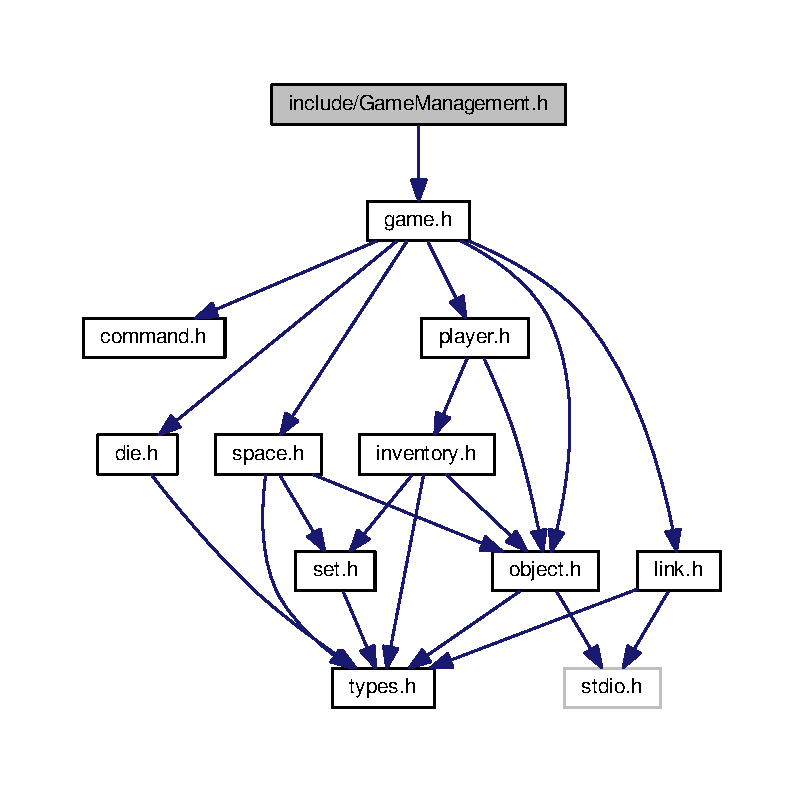
\includegraphics[width=350pt]{GameManagement_8h__incl}
\end{center}
\end{figure}
This graph shows which files directly or indirectly include this file\+:
\nopagebreak
\begin{figure}[H]
\begin{center}
\leavevmode
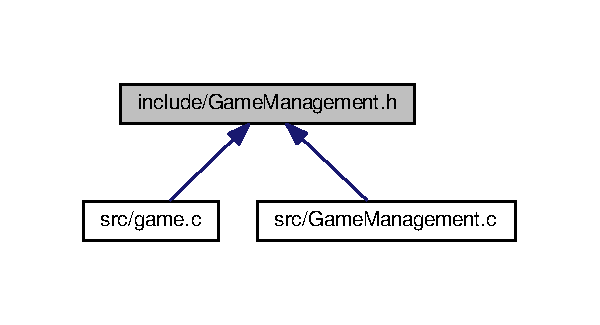
\includegraphics[width=288pt]{GameManagement_8h__dep__incl}
\end{center}
\end{figure}
\subsection*{Functions}
\begin{DoxyCompactItemize}
\item 
\hyperlink{types_8h_a32c27cc471df37f4fc818d65de0a56c4}{S\+T\+A\+T\+US} \hyperlink{GameManagement_8h_a51753ca919dffdc97f2249bd5edc4fa5}{game\+\_\+management\+\_\+load\+\_\+spaces} (\hyperlink{game_8h_a57156d39c530aec3fba3a9dad8c2dc6a}{Game} $\ast$game, char $\ast$filename)
\begin{DoxyCompactList}\small\item\em loads the spaces \end{DoxyCompactList}\item 
\hyperlink{types_8h_a32c27cc471df37f4fc818d65de0a56c4}{S\+T\+A\+T\+US} \hyperlink{GameManagement_8h_a59fad5fbf3d2f209ff5ab55060ad6974}{game\+\_\+management\+\_\+load\+\_\+objects} (\hyperlink{game_8h_a57156d39c530aec3fba3a9dad8c2dc6a}{Game} $\ast$game, char $\ast$filename)
\begin{DoxyCompactList}\small\item\em loads the objects \end{DoxyCompactList}\item 
\hyperlink{types_8h_a32c27cc471df37f4fc818d65de0a56c4}{S\+T\+A\+T\+US} \hyperlink{GameManagement_8h_a784e0d137d6ffdade3b65165be3a24bc}{game\+\_\+management\+\_\+load\+\_\+links} (\hyperlink{game_8h_a57156d39c530aec3fba3a9dad8c2dc6a}{Game} $\ast$game, char $\ast$filename)
\begin{DoxyCompactList}\small\item\em loads the links \end{DoxyCompactList}\item 
\hyperlink{types_8h_a32c27cc471df37f4fc818d65de0a56c4}{S\+T\+A\+T\+US} \hyperlink{GameManagement_8h_a7deb885075e008a0f2637330ce753047}{game\+\_\+management\+\_\+save\+\_\+game} (\hyperlink{game_8h_a57156d39c530aec3fba3a9dad8c2dc6a}{Game} $\ast$game, char $\ast$filename)
\begin{DoxyCompactList}\small\item\em saves the game \end{DoxyCompactList}\item 
\hyperlink{types_8h_a32c27cc471df37f4fc818d65de0a56c4}{S\+T\+A\+T\+US} \hyperlink{GameManagement_8h_afc72ef5dcc7b540e92ce2bec4fc0c466}{game\+\_\+management\+\_\+load\+\_\+game} (\hyperlink{game_8h_a57156d39c530aec3fba3a9dad8c2dc6a}{Game} $\ast$game, char $\ast$filename)
\begin{DoxyCompactList}\small\item\em saves the game \end{DoxyCompactList}\end{DoxyCompactItemize}


\subsection{Detailed Description}
Contains the declaration for game\+\_\+reader.\+c functions. 

\begin{DoxyAuthor}{Author}
Borja Pérez 
\end{DoxyAuthor}
\begin{DoxyVersion}{Version}
2.\+0 
\end{DoxyVersion}
\begin{DoxyDate}{Date}
29-\/04-\/2018 
\end{DoxyDate}


\subsection{Function Documentation}
\index{Game\+Management.\+h@{Game\+Management.\+h}!game\+\_\+management\+\_\+load\+\_\+game@{game\+\_\+management\+\_\+load\+\_\+game}}
\index{game\+\_\+management\+\_\+load\+\_\+game@{game\+\_\+management\+\_\+load\+\_\+game}!Game\+Management.\+h@{Game\+Management.\+h}}
\subsubsection[{\texorpdfstring{game\+\_\+management\+\_\+load\+\_\+game(\+Game $\ast$game, char $\ast$filename)}{game_management_load_game(Game *game, char *filename)}}]{\setlength{\rightskip}{0pt plus 5cm}{\bf S\+T\+A\+T\+US} game\+\_\+management\+\_\+load\+\_\+game (
\begin{DoxyParamCaption}
\item[{{\bf Game} $\ast$}]{game, }
\item[{char $\ast$}]{filename}
\end{DoxyParamCaption}
)}\hypertarget{GameManagement_8h_afc72ef5dcc7b540e92ce2bec4fc0c466}{}\label{GameManagement_8h_afc72ef5dcc7b540e92ce2bec4fc0c466}


saves the game 

Function used to load the currect game positioning of objects, spaces, etc. and loads a new file

\begin{DoxyAuthor}{Author}
Borja Pérez 
\end{DoxyAuthor}

\begin{DoxyParams}{Parameters}
{\em game} & a pointer to the game. \\
\hline
{\em filename} & a string with the name of the file from where the game is load. \\
\hline
\end{DoxyParams}
\begin{DoxyReturn}{Returns}
S\+T\+A\+T\+US, E\+R\+R\+OR if argument received is N\+U\+LL, if not, OK. 
\end{DoxyReturn}
\index{Game\+Management.\+h@{Game\+Management.\+h}!game\+\_\+management\+\_\+load\+\_\+links@{game\+\_\+management\+\_\+load\+\_\+links}}
\index{game\+\_\+management\+\_\+load\+\_\+links@{game\+\_\+management\+\_\+load\+\_\+links}!Game\+Management.\+h@{Game\+Management.\+h}}
\subsubsection[{\texorpdfstring{game\+\_\+management\+\_\+load\+\_\+links(\+Game $\ast$game, char $\ast$filename)}{game_management_load_links(Game *game, char *filename)}}]{\setlength{\rightskip}{0pt plus 5cm}{\bf S\+T\+A\+T\+US} game\+\_\+management\+\_\+load\+\_\+links (
\begin{DoxyParamCaption}
\item[{{\bf Game} $\ast$}]{game, }
\item[{char $\ast$}]{filename}
\end{DoxyParamCaption}
)}\hypertarget{GameManagement_8h_a784e0d137d6ffdade3b65165be3a24bc}{}\label{GameManagement_8h_a784e0d137d6ffdade3b65165be3a24bc}


loads the links 

Detects links in a file (P.\+E. data.\+dat) and loads them into a game

\begin{DoxyAuthor}{Author}
Borja Pérez 
\end{DoxyAuthor}

\begin{DoxyParams}{Parameters}
{\em game} & a pointer to the game where the links will be loaded. \\
\hline
{\em filename} & a string with the name of the file in where the links are saved. \\
\hline
\end{DoxyParams}
\begin{DoxyReturn}{Returns}
S\+T\+A\+T\+US, E\+R\+R\+OR if argument received is N\+U\+LL, if not, OK. 
\end{DoxyReturn}
\index{Game\+Management.\+h@{Game\+Management.\+h}!game\+\_\+management\+\_\+load\+\_\+objects@{game\+\_\+management\+\_\+load\+\_\+objects}}
\index{game\+\_\+management\+\_\+load\+\_\+objects@{game\+\_\+management\+\_\+load\+\_\+objects}!Game\+Management.\+h@{Game\+Management.\+h}}
\subsubsection[{\texorpdfstring{game\+\_\+management\+\_\+load\+\_\+objects(\+Game $\ast$game, char $\ast$filename)}{game_management_load_objects(Game *game, char *filename)}}]{\setlength{\rightskip}{0pt plus 5cm}{\bf S\+T\+A\+T\+US} game\+\_\+management\+\_\+load\+\_\+objects (
\begin{DoxyParamCaption}
\item[{{\bf Game} $\ast$}]{game, }
\item[{char $\ast$}]{filename}
\end{DoxyParamCaption}
)}\hypertarget{GameManagement_8h_a59fad5fbf3d2f209ff5ab55060ad6974}{}\label{GameManagement_8h_a59fad5fbf3d2f209ff5ab55060ad6974}


loads the objects 

Detects objects in a file (P.\+E. data.\+dat) and loads them into a game

\begin{DoxyAuthor}{Author}
Borja Pérez 
\end{DoxyAuthor}

\begin{DoxyParams}{Parameters}
{\em game} & a pointer to the game where the objects will be loaded. \\
\hline
{\em filename} & a string with the name of the file in where the objects are saved. \\
\hline
\end{DoxyParams}
\begin{DoxyReturn}{Returns}
S\+T\+A\+T\+US, E\+R\+R\+OR if argument received is N\+U\+LL, if not, OK. 
\end{DoxyReturn}
\index{Game\+Management.\+h@{Game\+Management.\+h}!game\+\_\+management\+\_\+load\+\_\+spaces@{game\+\_\+management\+\_\+load\+\_\+spaces}}
\index{game\+\_\+management\+\_\+load\+\_\+spaces@{game\+\_\+management\+\_\+load\+\_\+spaces}!Game\+Management.\+h@{Game\+Management.\+h}}
\subsubsection[{\texorpdfstring{game\+\_\+management\+\_\+load\+\_\+spaces(\+Game $\ast$game, char $\ast$filename)}{game_management_load_spaces(Game *game, char *filename)}}]{\setlength{\rightskip}{0pt plus 5cm}{\bf S\+T\+A\+T\+US} game\+\_\+management\+\_\+load\+\_\+spaces (
\begin{DoxyParamCaption}
\item[{{\bf Game} $\ast$}]{game, }
\item[{char $\ast$}]{filename}
\end{DoxyParamCaption}
)}\hypertarget{GameManagement_8h_a51753ca919dffdc97f2249bd5edc4fa5}{}\label{GameManagement_8h_a51753ca919dffdc97f2249bd5edc4fa5}


loads the spaces 

Detects spaces in a file (P.\+E. data.\+dat) and loads them into a game.

\begin{DoxyAuthor}{Author}
Borja Pérez 
\end{DoxyAuthor}

\begin{DoxyParams}{Parameters}
{\em game} & a pointer to the game where the spaces will be loaded. \\
\hline
{\em filename} & a string with the name of the file in where the spaces are saved. \\
\hline
\end{DoxyParams}
\begin{DoxyReturn}{Returns}
S\+T\+A\+T\+US, E\+R\+R\+OR if argument received is N\+U\+LL, if not, OK. 
\end{DoxyReturn}
\index{Game\+Management.\+h@{Game\+Management.\+h}!game\+\_\+management\+\_\+save\+\_\+game@{game\+\_\+management\+\_\+save\+\_\+game}}
\index{game\+\_\+management\+\_\+save\+\_\+game@{game\+\_\+management\+\_\+save\+\_\+game}!Game\+Management.\+h@{Game\+Management.\+h}}
\subsubsection[{\texorpdfstring{game\+\_\+management\+\_\+save\+\_\+game(\+Game $\ast$game, char $\ast$filename)}{game_management_save_game(Game *game, char *filename)}}]{\setlength{\rightskip}{0pt plus 5cm}{\bf S\+T\+A\+T\+US} game\+\_\+management\+\_\+save\+\_\+game (
\begin{DoxyParamCaption}
\item[{{\bf Game} $\ast$}]{game, }
\item[{char $\ast$}]{filename}
\end{DoxyParamCaption}
)}\hypertarget{GameManagement_8h_a7deb885075e008a0f2637330ce753047}{}\label{GameManagement_8h_a7deb885075e008a0f2637330ce753047}


saves the game 

Function used to save the currect game positioning of objects, spaces, etc. and creates a new file

\begin{DoxyAuthor}{Author}
Borja Pérez 
\end{DoxyAuthor}

\begin{DoxyParams}{Parameters}
{\em game} & a pointer to the game. \\
\hline
{\em filename} & a string with the name of the file in where the game is saved. \\
\hline
\end{DoxyParams}
\begin{DoxyReturn}{Returns}
S\+T\+A\+T\+US, E\+R\+R\+OR if argument received is N\+U\+LL, if not, OK. 
\end{DoxyReturn}

\hypertarget{graphic__engine_8h}{}\section{include/graphic\+\_\+engine.h File Reference}
\label{graphic__engine_8h}\index{include/graphic\+\_\+engine.\+h@{include/graphic\+\_\+engine.\+h}}


defines the graphic engine  


{\ttfamily \#include \char`\"{}game.\+h\char`\"{}}\\*
Include dependency graph for graphic\+\_\+engine.\+h\+:
\nopagebreak
\begin{figure}[H]
\begin{center}
\leavevmode
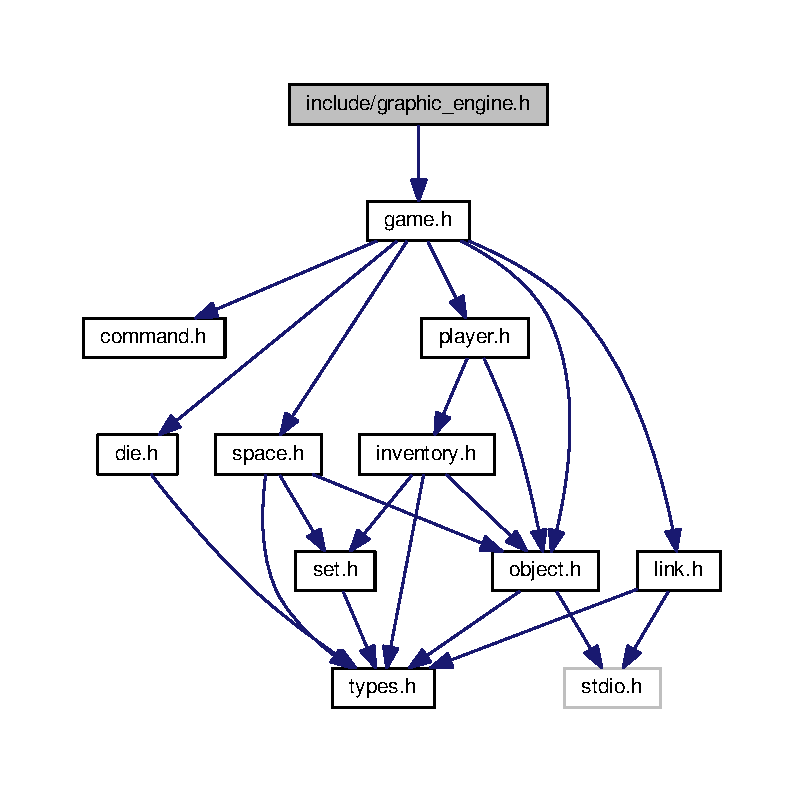
\includegraphics[width=350pt]{graphic__engine_8h__incl}
\end{center}
\end{figure}
This graph shows which files directly or indirectly include this file\+:
\nopagebreak
\begin{figure}[H]
\begin{center}
\leavevmode
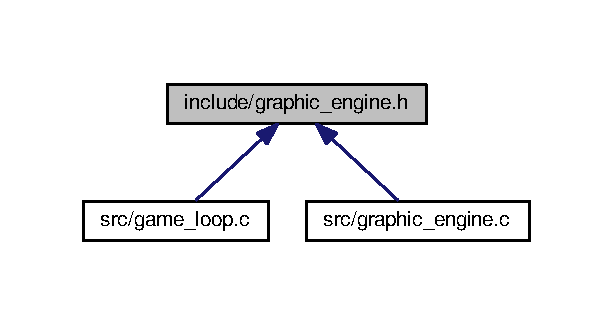
\includegraphics[width=294pt]{graphic__engine_8h__dep__incl}
\end{center}
\end{figure}
\subsection*{Typedefs}
\begin{DoxyCompactItemize}
\item 
typedef struct \hyperlink{struct__Graphic__engine}{\+\_\+\+Graphic\+\_\+engine} \hyperlink{graphic__engine_8h_ae1bc5cdbfce93098f066274fdea49af1}{Graphic\+\_\+engine}
\begin{DoxyCompactList}\small\item\em graphic design \end{DoxyCompactList}\end{DoxyCompactItemize}
\subsection*{Functions}
\begin{DoxyCompactItemize}
\item 
\hyperlink{graphic__engine_8h_ae1bc5cdbfce93098f066274fdea49af1}{Graphic\+\_\+engine} $\ast$ \hyperlink{graphic__engine_8h_a8c3d9abe7282bee1d77d23ea80a4bdec}{graphic\+\_\+engine\+\_\+create} ()
\begin{DoxyCompactList}\small\item\em creates the graphic engine \end{DoxyCompactList}\item 
void \hyperlink{graphic__engine_8h_a5a5eac4ef2033c5ad71aa6895f362f79}{graphic\+\_\+engine\+\_\+destroy} (\hyperlink{graphic__engine_8h_ae1bc5cdbfce93098f066274fdea49af1}{Graphic\+\_\+engine} $\ast$ge)
\begin{DoxyCompactList}\small\item\em frees memory \end{DoxyCompactList}\item 
void \hyperlink{graphic__engine_8h_a0e275aa477d5fa59e903da33a2a40a5d}{graphic\+\_\+engine\+\_\+paint\+\_\+game} (\hyperlink{graphic__engine_8h_ae1bc5cdbfce93098f066274fdea49af1}{Graphic\+\_\+engine} $\ast$ge, \hyperlink{game_8h_a57156d39c530aec3fba3a9dad8c2dc6a}{Game} $\ast$game)
\begin{DoxyCompactList}\small\item\em paints the game \end{DoxyCompactList}\item 
void \hyperlink{graphic__engine_8h_a112605879db4582a6d9cd6c12bd0e90c}{graphic\+\_\+engine\+\_\+write\+\_\+command} (\hyperlink{graphic__engine_8h_ae1bc5cdbfce93098f066274fdea49af1}{Graphic\+\_\+engine} $\ast$ge, char $\ast$str)
\begin{DoxyCompactList}\small\item\em writes the commands \end{DoxyCompactList}\end{DoxyCompactItemize}


\subsection{Detailed Description}
defines the graphic engine 

\begin{DoxyAuthor}{Author}
Dan Roife 
\end{DoxyAuthor}
\begin{DoxyVersion}{Version}
2.\+0 
\end{DoxyVersion}
\begin{DoxyDate}{Date}
07-\/04-\/2018 
\end{DoxyDate}


\subsection{Typedef Documentation}
\index{graphic\+\_\+engine.\+h@{graphic\+\_\+engine.\+h}!Graphic\+\_\+engine@{Graphic\+\_\+engine}}
\index{Graphic\+\_\+engine@{Graphic\+\_\+engine}!graphic\+\_\+engine.\+h@{graphic\+\_\+engine.\+h}}
\subsubsection[{\texorpdfstring{Graphic\+\_\+engine}{Graphic_engine}}]{\setlength{\rightskip}{0pt plus 5cm}typedef struct {\bf \+\_\+\+Graphic\+\_\+engine} {\bf Graphic\+\_\+engine}}\hypertarget{graphic__engine_8h_ae1bc5cdbfce93098f066274fdea49af1}{}\label{graphic__engine_8h_ae1bc5cdbfce93098f066274fdea49af1}


graphic design 

Struct that include the variables that will help us show the design of our game. 

\subsection{Function Documentation}
\index{graphic\+\_\+engine.\+h@{graphic\+\_\+engine.\+h}!graphic\+\_\+engine\+\_\+create@{graphic\+\_\+engine\+\_\+create}}
\index{graphic\+\_\+engine\+\_\+create@{graphic\+\_\+engine\+\_\+create}!graphic\+\_\+engine.\+h@{graphic\+\_\+engine.\+h}}
\subsubsection[{\texorpdfstring{graphic\+\_\+engine\+\_\+create()}{graphic_engine_create()}}]{\setlength{\rightskip}{0pt plus 5cm}{\bf Graphic\+\_\+engine}$\ast$ graphic\+\_\+engine\+\_\+create (
\begin{DoxyParamCaption}
{}
\end{DoxyParamCaption}
)}\hypertarget{graphic__engine_8h_a8c3d9abe7282bee1d77d23ea80a4bdec}{}\label{graphic__engine_8h_a8c3d9abe7282bee1d77d23ea80a4bdec}


creates the graphic engine 

Allocates the memory for a new graphic engine and declares its parts

\begin{DoxyAuthor}{Author}
Dan Roife 
\end{DoxyAuthor}
\begin{DoxyReturn}{Returns}
pointer to a graphic engine. 
\end{DoxyReturn}
\index{graphic\+\_\+engine.\+h@{graphic\+\_\+engine.\+h}!graphic\+\_\+engine\+\_\+destroy@{graphic\+\_\+engine\+\_\+destroy}}
\index{graphic\+\_\+engine\+\_\+destroy@{graphic\+\_\+engine\+\_\+destroy}!graphic\+\_\+engine.\+h@{graphic\+\_\+engine.\+h}}
\subsubsection[{\texorpdfstring{graphic\+\_\+engine\+\_\+destroy(\+Graphic\+\_\+engine $\ast$ge)}{graphic_engine_destroy(Graphic_engine *ge)}}]{\setlength{\rightskip}{0pt plus 5cm}void graphic\+\_\+engine\+\_\+destroy (
\begin{DoxyParamCaption}
\item[{{\bf Graphic\+\_\+engine} $\ast$}]{ge}
\end{DoxyParamCaption}
)}\hypertarget{graphic__engine_8h_a5a5eac4ef2033c5ad71aa6895f362f79}{}\label{graphic__engine_8h_a5a5eac4ef2033c5ad71aa6895f362f79}


frees memory 

Frees the memory allocated for the graphic engine and its parts.

\begin{DoxyAuthor}{Author}
Dan Roife 
\end{DoxyAuthor}

\begin{DoxyParams}{Parameters}
{\em ge} & pointer to graphic engine. \\
\hline
\end{DoxyParams}
\begin{DoxyReturn}{Returns}
void function. 
\end{DoxyReturn}
\index{graphic\+\_\+engine.\+h@{graphic\+\_\+engine.\+h}!graphic\+\_\+engine\+\_\+paint\+\_\+game@{graphic\+\_\+engine\+\_\+paint\+\_\+game}}
\index{graphic\+\_\+engine\+\_\+paint\+\_\+game@{graphic\+\_\+engine\+\_\+paint\+\_\+game}!graphic\+\_\+engine.\+h@{graphic\+\_\+engine.\+h}}
\subsubsection[{\texorpdfstring{graphic\+\_\+engine\+\_\+paint\+\_\+game(\+Graphic\+\_\+engine $\ast$ge, Game $\ast$game)}{graphic_engine_paint_game(Graphic_engine *ge, Game *game)}}]{\setlength{\rightskip}{0pt plus 5cm}void graphic\+\_\+engine\+\_\+paint\+\_\+game (
\begin{DoxyParamCaption}
\item[{{\bf Graphic\+\_\+engine} $\ast$}]{ge, }
\item[{{\bf Game} $\ast$}]{game}
\end{DoxyParamCaption}
)}\hypertarget{graphic__engine_8h_a0e275aa477d5fa59e903da33a2a40a5d}{}\label{graphic__engine_8h_a0e275aa477d5fa59e903da33a2a40a5d}


paints the game 

Shows a graphic interface with the contents of the game.

\begin{DoxyAuthor}{Author}
Dan Roife 
\end{DoxyAuthor}

\begin{DoxyParams}{Parameters}
{\em ge} & pointer to graphic engine. \\
\hline
{\em game} & pointer to game. \\
\hline
\end{DoxyParams}
\begin{DoxyReturn}{Returns}
void function. 
\end{DoxyReturn}
\index{graphic\+\_\+engine.\+h@{graphic\+\_\+engine.\+h}!graphic\+\_\+engine\+\_\+write\+\_\+command@{graphic\+\_\+engine\+\_\+write\+\_\+command}}
\index{graphic\+\_\+engine\+\_\+write\+\_\+command@{graphic\+\_\+engine\+\_\+write\+\_\+command}!graphic\+\_\+engine.\+h@{graphic\+\_\+engine.\+h}}
\subsubsection[{\texorpdfstring{graphic\+\_\+engine\+\_\+write\+\_\+command(\+Graphic\+\_\+engine $\ast$ge, char $\ast$str)}{graphic_engine_write_command(Graphic_engine *ge, char *str)}}]{\setlength{\rightskip}{0pt plus 5cm}void graphic\+\_\+engine\+\_\+write\+\_\+command (
\begin{DoxyParamCaption}
\item[{{\bf Graphic\+\_\+engine} $\ast$}]{ge, }
\item[{char $\ast$}]{str}
\end{DoxyParamCaption}
)}\hypertarget{graphic__engine_8h_a112605879db4582a6d9cd6c12bd0e90c}{}\label{graphic__engine_8h_a112605879db4582a6d9cd6c12bd0e90c}


writes the commands 

Enables us to write the command that we want to use in a certain moment.

\begin{DoxyAuthor}{Author}
Dan Roife 
\end{DoxyAuthor}

\begin{DoxyParams}{Parameters}
{\em ge} & pointer to graphic engine. \\
\hline
{\em str} & string. \\
\hline
\end{DoxyParams}
\begin{DoxyReturn}{Returns}
void function. 
\end{DoxyReturn}

\hypertarget{inventory_8h}{}\section{include/inventory.h File Reference}
\label{inventory_8h}\index{include/inventory.\+h@{include/inventory.\+h}}


organises the objects in a backpack  


{\ttfamily \#include \char`\"{}types.\+h\char`\"{}}\\*
{\ttfamily \#include \char`\"{}object.\+h\char`\"{}}\\*
{\ttfamily \#include \char`\"{}set.\+h\char`\"{}}\\*
Include dependency graph for inventory.\+h\+:
\nopagebreak
\begin{figure}[H]
\begin{center}
\leavevmode
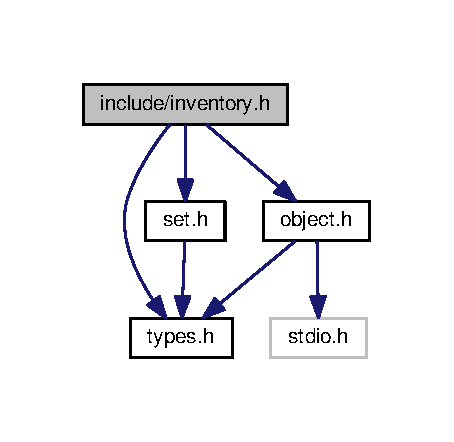
\includegraphics[width=218pt]{inventory_8h__incl}
\end{center}
\end{figure}
This graph shows which files directly or indirectly include this file\+:
\nopagebreak
\begin{figure}[H]
\begin{center}
\leavevmode
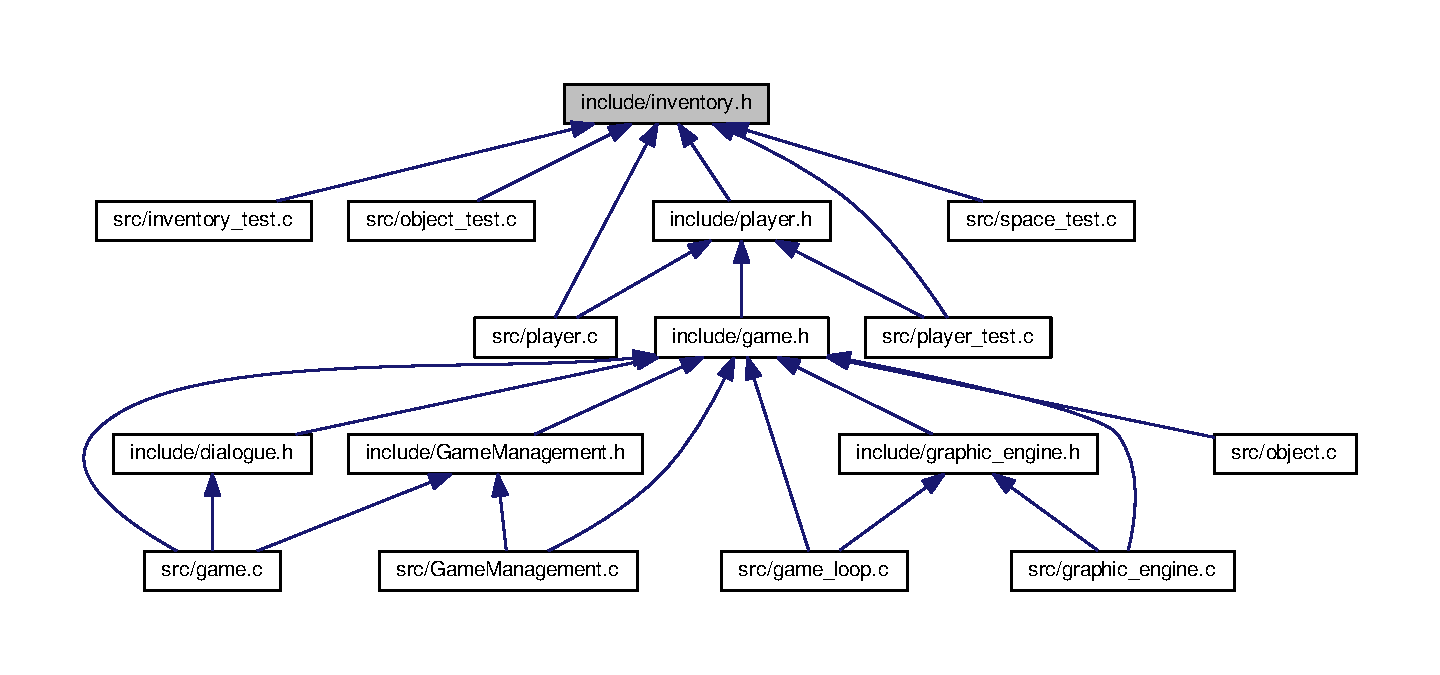
\includegraphics[width=350pt]{inventory_8h__dep__incl}
\end{center}
\end{figure}
\subsection*{Typedefs}
\begin{DoxyCompactItemize}
\item 
typedef struct \hyperlink{struct__Inventory}{\+\_\+\+Inventory} \hyperlink{inventory_8h_a2253bf64ac4ce6a9c1d6f39c0b0d32a3}{Inventory}
\begin{DoxyCompactList}\small\item\em set and max objects. \end{DoxyCompactList}\end{DoxyCompactItemize}
\subsection*{Functions}
\begin{DoxyCompactItemize}
\item 
\hyperlink{inventory_8h_a2253bf64ac4ce6a9c1d6f39c0b0d32a3}{Inventory} $\ast$ \hyperlink{inventory_8h_a5d6b47f7a727932c56d66a65fb540910}{inventory\+\_\+create} ()
\begin{DoxyCompactList}\small\item\em creates an inventory \end{DoxyCompactList}\item 
\hyperlink{types_8h_a32c27cc471df37f4fc818d65de0a56c4}{S\+T\+A\+T\+US} \hyperlink{inventory_8h_a670571ee9591b73ca5dfbc0b79b45882}{inventory\+\_\+destroy} (\hyperlink{inventory_8h_a2253bf64ac4ce6a9c1d6f39c0b0d32a3}{Inventory} $\ast$inv)
\begin{DoxyCompactList}\small\item\em frees memory \end{DoxyCompactList}\item 
\hyperlink{types_8h_a32c27cc471df37f4fc818d65de0a56c4}{S\+T\+A\+T\+US} \hyperlink{inventory_8h_a91549cebec2fd5c6f3ec0c7d6448dc31}{inventory\+\_\+add\+\_\+id} (\hyperlink{inventory_8h_a2253bf64ac4ce6a9c1d6f39c0b0d32a3}{Inventory} $\ast$inv, \hyperlink{types_8h_a845e604fb28f7e3d97549da3448149d3}{Id} id)
\begin{DoxyCompactList}\small\item\em adds an id \end{DoxyCompactList}\item 
\hyperlink{types_8h_a32c27cc471df37f4fc818d65de0a56c4}{S\+T\+A\+T\+US} \hyperlink{inventory_8h_a3e4734307f0bc60bdb14a432328495f7}{inventory\+\_\+delete\+\_\+id} (\hyperlink{inventory_8h_a2253bf64ac4ce6a9c1d6f39c0b0d32a3}{Inventory} $\ast$inv, \hyperlink{types_8h_a845e604fb28f7e3d97549da3448149d3}{Id} id)
\begin{DoxyCompactList}\small\item\em deletes and id \end{DoxyCompactList}\item 
\hyperlink{types_8h_a845e604fb28f7e3d97549da3448149d3}{Id} \hyperlink{inventory_8h_a5d7d0f3bbe7439f1f7e47f3cf4acc704}{inventory\+\_\+get\+\_\+object} (\hyperlink{inventory_8h_a2253bf64ac4ce6a9c1d6f39c0b0d32a3}{Inventory} $\ast$inv, int position)
\begin{DoxyCompactList}\small\item\em gets the id of an object \end{DoxyCompactList}\item 
\hyperlink{types_8h_a3e5b8192e7d9ffaf3542f1210aec18dd}{B\+O\+OL} \hyperlink{inventory_8h_a49a57de1417c72d6a976a31af7ed9f33}{inventory\+\_\+has\+\_\+object} (\hyperlink{inventory_8h_a2253bf64ac4ce6a9c1d6f39c0b0d32a3}{Inventory} $\ast$inv, \hyperlink{types_8h_a845e604fb28f7e3d97549da3448149d3}{Id} id)
\begin{DoxyCompactList}\small\item\em checks if there is an object in the inventory \end{DoxyCompactList}\item 
\hyperlink{set_8h_a6d3b7f7c92cbb4577ef3ef7ddbf93161}{Set} $\ast$ \hyperlink{inventory_8h_a4b9a14258433fc87eadf9354547ab938}{inventory\+\_\+get\+\_\+set} (\hyperlink{inventory_8h_a2253bf64ac4ce6a9c1d6f39c0b0d32a3}{Inventory} $\ast$inv)
\begin{DoxyCompactList}\small\item\em gets and id using pointer to set \end{DoxyCompactList}\item 
\hyperlink{types_8h_a32c27cc471df37f4fc818d65de0a56c4}{S\+T\+A\+T\+US} \hyperlink{inventory_8h_a7e6e5fac8c72945a9022ff69772cb72c}{inventory\+\_\+print} (\hyperlink{inventory_8h_a2253bf64ac4ce6a9c1d6f39c0b0d32a3}{Inventory} $\ast$inv)
\begin{DoxyCompactList}\small\item\em prints the inventory \end{DoxyCompactList}\item 
\hyperlink{types_8h_a3e5b8192e7d9ffaf3542f1210aec18dd}{B\+O\+OL} \hyperlink{inventory_8h_a294538bee7ebbc19c120d63a6bc603cf}{inventory\+\_\+is\+\_\+empty} (\hyperlink{inventory_8h_a2253bf64ac4ce6a9c1d6f39c0b0d32a3}{Inventory} $\ast$inv)
\begin{DoxyCompactList}\small\item\em checks if the inventory is empty \end{DoxyCompactList}\item 
\hyperlink{types_8h_a3e5b8192e7d9ffaf3542f1210aec18dd}{B\+O\+OL} \hyperlink{inventory_8h_a046e96fa72b449e8efca96fee6a33062}{inventory\+\_\+is\+\_\+full} (\hyperlink{inventory_8h_a2253bf64ac4ce6a9c1d6f39c0b0d32a3}{Inventory} $\ast$inv)
\begin{DoxyCompactList}\small\item\em checks if the inventory is full \end{DoxyCompactList}\end{DoxyCompactItemize}


\subsection{Detailed Description}
organises the objects in a backpack 

This module helps the organisation and the managing of the objects by using different functions that enables the player to work with an inventory of objects.

\begin{DoxyAuthor}{Author}
Juan Moreno 
\end{DoxyAuthor}
\begin{DoxyVersion}{Version}
1.\+0 
\end{DoxyVersion}
\begin{DoxyDate}{Date}
05-\/04-\/2018 
\end{DoxyDate}


\subsection{Typedef Documentation}
\index{inventory.\+h@{inventory.\+h}!Inventory@{Inventory}}
\index{Inventory@{Inventory}!inventory.\+h@{inventory.\+h}}
\subsubsection[{\texorpdfstring{Inventory}{Inventory}}]{\setlength{\rightskip}{0pt plus 5cm}typedef struct {\bf \+\_\+\+Inventory} {\bf Inventory}}\hypertarget{inventory_8h_a2253bf64ac4ce6a9c1d6f39c0b0d32a3}{}\label{inventory_8h_a2253bf64ac4ce6a9c1d6f39c0b0d32a3}


set and max objects. 

Struct for organising the objects using a pointer to set and a maximum number of objects(int). 

\subsection{Function Documentation}
\index{inventory.\+h@{inventory.\+h}!inventory\+\_\+add\+\_\+id@{inventory\+\_\+add\+\_\+id}}
\index{inventory\+\_\+add\+\_\+id@{inventory\+\_\+add\+\_\+id}!inventory.\+h@{inventory.\+h}}
\subsubsection[{\texorpdfstring{inventory\+\_\+add\+\_\+id(\+Inventory $\ast$inv, Id id)}{inventory_add_id(Inventory *inv, Id id)}}]{\setlength{\rightskip}{0pt plus 5cm}{\bf S\+T\+A\+T\+US} inventory\+\_\+add\+\_\+id (
\begin{DoxyParamCaption}
\item[{{\bf Inventory} $\ast$}]{inv, }
\item[{{\bf Id}}]{id}
\end{DoxyParamCaption}
)}\hypertarget{inventory_8h_a91549cebec2fd5c6f3ec0c7d6448dc31}{}\label{inventory_8h_a91549cebec2fd5c6f3ec0c7d6448dc31}


adds an id 

It is the function in charge of adding ids to the inventory by using the appropriate set function.

\begin{DoxyAuthor}{Author}
Juan Moreno 
\end{DoxyAuthor}

\begin{DoxyParams}{Parameters}
{\em inv} & pointer to inventory. \\
\hline
{\em id} & long int. \\
\hline
\end{DoxyParams}
\begin{DoxyReturn}{Returns}
S\+T\+A\+T\+US, E\+R\+R\+OR if argument received is N\+U\+LL, if not, OK. 
\end{DoxyReturn}
\index{inventory.\+h@{inventory.\+h}!inventory\+\_\+create@{inventory\+\_\+create}}
\index{inventory\+\_\+create@{inventory\+\_\+create}!inventory.\+h@{inventory.\+h}}
\subsubsection[{\texorpdfstring{inventory\+\_\+create()}{inventory_create()}}]{\setlength{\rightskip}{0pt plus 5cm}{\bf Inventory}$\ast$ inventory\+\_\+create (
\begin{DoxyParamCaption}
{}
\end{DoxyParamCaption}
)}\hypertarget{inventory_8h_a5d6b47f7a727932c56d66a65fb540910}{}\label{inventory_8h_a5d6b47f7a727932c56d66a65fb540910}


creates an inventory 

It creates a new inventory initializing the variables of the structure, checks is something goes wrong and if it does go wrong, returns N\+U\+LL.

\begin{DoxyAuthor}{Author}
Juan Moreno 
\end{DoxyAuthor}
\begin{DoxyReturn}{Returns}
Pointer to inventory, N\+U\+LL if something goes wrong. 
\end{DoxyReturn}
\index{inventory.\+h@{inventory.\+h}!inventory\+\_\+delete\+\_\+id@{inventory\+\_\+delete\+\_\+id}}
\index{inventory\+\_\+delete\+\_\+id@{inventory\+\_\+delete\+\_\+id}!inventory.\+h@{inventory.\+h}}
\subsubsection[{\texorpdfstring{inventory\+\_\+delete\+\_\+id(\+Inventory $\ast$inv, Id id)}{inventory_delete_id(Inventory *inv, Id id)}}]{\setlength{\rightskip}{0pt plus 5cm}{\bf S\+T\+A\+T\+US} inventory\+\_\+delete\+\_\+id (
\begin{DoxyParamCaption}
\item[{{\bf Inventory} $\ast$}]{inv, }
\item[{{\bf Id}}]{id}
\end{DoxyParamCaption}
)}\hypertarget{inventory_8h_a3e4734307f0bc60bdb14a432328495f7}{}\label{inventory_8h_a3e4734307f0bc60bdb14a432328495f7}


deletes and id 

Function in charge of deleting and id of the inventory that you have already added when it is necessary.

\begin{DoxyAuthor}{Author}
Juan Moreno 
\end{DoxyAuthor}

\begin{DoxyParams}{Parameters}
{\em inv} & pointer to inventory. \\
\hline
{\em id} & long int. \\
\hline
\end{DoxyParams}
\begin{DoxyReturn}{Returns}
S\+T\+A\+T\+US, E\+R\+R\+OR if argument received is N\+U\+LL, if not, OK. 
\end{DoxyReturn}
\index{inventory.\+h@{inventory.\+h}!inventory\+\_\+destroy@{inventory\+\_\+destroy}}
\index{inventory\+\_\+destroy@{inventory\+\_\+destroy}!inventory.\+h@{inventory.\+h}}
\subsubsection[{\texorpdfstring{inventory\+\_\+destroy(\+Inventory $\ast$inv)}{inventory_destroy(Inventory *inv)}}]{\setlength{\rightskip}{0pt plus 5cm}{\bf S\+T\+A\+T\+US} inventory\+\_\+destroy (
\begin{DoxyParamCaption}
\item[{{\bf Inventory} $\ast$}]{inv}
\end{DoxyParamCaption}
)}\hypertarget{inventory_8h_a670571ee9591b73ca5dfbc0b79b45882}{}\label{inventory_8h_a670571ee9591b73ca5dfbc0b79b45882}


frees memory 

Receives pointer to inventory and frees the memory it occupied.

\begin{DoxyAuthor}{Author}
Juan Moreno 
\end{DoxyAuthor}

\begin{DoxyParams}{Parameters}
{\em inv} & pointer to inventory. \\
\hline
\end{DoxyParams}
\begin{DoxyReturn}{Returns}
S\+T\+A\+T\+US, E\+R\+R\+OR if argument received is N\+U\+LL, if not, OK. 
\end{DoxyReturn}
\index{inventory.\+h@{inventory.\+h}!inventory\+\_\+get\+\_\+object@{inventory\+\_\+get\+\_\+object}}
\index{inventory\+\_\+get\+\_\+object@{inventory\+\_\+get\+\_\+object}!inventory.\+h@{inventory.\+h}}
\subsubsection[{\texorpdfstring{inventory\+\_\+get\+\_\+object(\+Inventory $\ast$inv, int position)}{inventory_get_object(Inventory *inv, int position)}}]{\setlength{\rightskip}{0pt plus 5cm}{\bf Id} inventory\+\_\+get\+\_\+object (
\begin{DoxyParamCaption}
\item[{{\bf Inventory} $\ast$}]{inv, }
\item[{int}]{position}
\end{DoxyParamCaption}
)}\hypertarget{inventory_8h_a5d7d0f3bbe7439f1f7e47f3cf4acc704}{}\label{inventory_8h_a5d7d0f3bbe7439f1f7e47f3cf4acc704}


gets the id of an object 

Function in charge of getting an object by using its id, that id is selected with a position (int).

\begin{DoxyAuthor}{Author}
Juan Moreno 
\end{DoxyAuthor}

\begin{DoxyParams}{Parameters}
{\em inv} & pointer to inventory. \\
\hline
{\em position} & position of the object (int). \\
\hline
\end{DoxyParams}
\begin{DoxyReturn}{Returns}
Id, N\+O\+\_\+\+ID if inventory is pointing N\+U\+LL. 
\end{DoxyReturn}
\index{inventory.\+h@{inventory.\+h}!inventory\+\_\+get\+\_\+set@{inventory\+\_\+get\+\_\+set}}
\index{inventory\+\_\+get\+\_\+set@{inventory\+\_\+get\+\_\+set}!inventory.\+h@{inventory.\+h}}
\subsubsection[{\texorpdfstring{inventory\+\_\+get\+\_\+set(\+Inventory $\ast$inv)}{inventory_get_set(Inventory *inv)}}]{\setlength{\rightskip}{0pt plus 5cm}{\bf Set}$\ast$ inventory\+\_\+get\+\_\+set (
\begin{DoxyParamCaption}
\item[{{\bf Inventory} $\ast$}]{inv}
\end{DoxyParamCaption}
)}\hypertarget{inventory_8h_a4b9a14258433fc87eadf9354547ab938}{}\label{inventory_8h_a4b9a14258433fc87eadf9354547ab938}


gets and id using pointer to set 

Function in which we will get the set of ids by using our pointer to set which is defined in the data structure.

\begin{DoxyAuthor}{Author}
Juan Moreno 
\end{DoxyAuthor}

\begin{DoxyParams}{Parameters}
{\em inv} & pointer to inventory. \\
\hline
\end{DoxyParams}
\begin{DoxyReturn}{Returns}
Pointer to inventory(set of ids). 
\end{DoxyReturn}
\index{inventory.\+h@{inventory.\+h}!inventory\+\_\+has\+\_\+object@{inventory\+\_\+has\+\_\+object}}
\index{inventory\+\_\+has\+\_\+object@{inventory\+\_\+has\+\_\+object}!inventory.\+h@{inventory.\+h}}
\subsubsection[{\texorpdfstring{inventory\+\_\+has\+\_\+object(\+Inventory $\ast$inv, Id id)}{inventory_has_object(Inventory *inv, Id id)}}]{\setlength{\rightskip}{0pt plus 5cm}{\bf B\+O\+OL} inventory\+\_\+has\+\_\+object (
\begin{DoxyParamCaption}
\item[{{\bf Inventory} $\ast$}]{inv, }
\item[{{\bf Id}}]{id}
\end{DoxyParamCaption}
)}\hypertarget{inventory_8h_a49a57de1417c72d6a976a31af7ed9f33}{}\label{inventory_8h_a49a57de1417c72d6a976a31af7ed9f33}


checks if there is an object in the inventory 

Function that, by calling the function\+: set\+\_\+has\+\_\+id can check that there is an object in the inventory using its id.

\begin{DoxyAuthor}{Author}
Juan Moreno 
\end{DoxyAuthor}

\begin{DoxyParams}{Parameters}
{\em inv} & pointer to inventory. \\
\hline
{\em id} & long int. \\
\hline
\end{DoxyParams}
\begin{DoxyReturn}{Returns}
B\+O\+OL, F\+A\+L\+SE if when checking is not correct, if it is correct, T\+R\+UE. 
\end{DoxyReturn}
\index{inventory.\+h@{inventory.\+h}!inventory\+\_\+is\+\_\+empty@{inventory\+\_\+is\+\_\+empty}}
\index{inventory\+\_\+is\+\_\+empty@{inventory\+\_\+is\+\_\+empty}!inventory.\+h@{inventory.\+h}}
\subsubsection[{\texorpdfstring{inventory\+\_\+is\+\_\+empty(\+Inventory $\ast$inv)}{inventory_is_empty(Inventory *inv)}}]{\setlength{\rightskip}{0pt plus 5cm}{\bf B\+O\+OL} inventory\+\_\+is\+\_\+empty (
\begin{DoxyParamCaption}
\item[{{\bf Inventory} $\ast$}]{inv}
\end{DoxyParamCaption}
)}\hypertarget{inventory_8h_a294538bee7ebbc19c120d63a6bc603cf}{}\label{inventory_8h_a294538bee7ebbc19c120d63a6bc603cf}


checks if the inventory is empty 

Function that will help us in other functions that need to check if there is any object in the inventory.

\begin{DoxyAuthor}{Author}
Juan Moreno 
\end{DoxyAuthor}

\begin{DoxyParams}{Parameters}
{\em inv} & pointer to inventory. \\
\hline
\end{DoxyParams}
\begin{DoxyReturn}{Returns}
B\+O\+OL, F\+A\+L\+SE if when checking is not correct, if it is correct, T\+R\+UE. 
\end{DoxyReturn}
\index{inventory.\+h@{inventory.\+h}!inventory\+\_\+is\+\_\+full@{inventory\+\_\+is\+\_\+full}}
\index{inventory\+\_\+is\+\_\+full@{inventory\+\_\+is\+\_\+full}!inventory.\+h@{inventory.\+h}}
\subsubsection[{\texorpdfstring{inventory\+\_\+is\+\_\+full(\+Inventory $\ast$inv)}{inventory_is_full(Inventory *inv)}}]{\setlength{\rightskip}{0pt plus 5cm}{\bf B\+O\+OL} inventory\+\_\+is\+\_\+full (
\begin{DoxyParamCaption}
\item[{{\bf Inventory} $\ast$}]{inv}
\end{DoxyParamCaption}
)}\hypertarget{inventory_8h_a046e96fa72b449e8efca96fee6a33062}{}\label{inventory_8h_a046e96fa72b449e8efca96fee6a33062}


checks if the inventory is full 

Function that will help us in other functions that need to check if the entire inventory is full of objects

\begin{DoxyAuthor}{Author}
Juan Moreno 
\end{DoxyAuthor}

\begin{DoxyParams}{Parameters}
{\em inv} & pointer to inventory. \\
\hline
\end{DoxyParams}
\begin{DoxyReturn}{Returns}
B\+O\+OL, F\+A\+L\+SE if when checking is not correct, if it is correct, T\+R\+UE. 
\end{DoxyReturn}
\index{inventory.\+h@{inventory.\+h}!inventory\+\_\+print@{inventory\+\_\+print}}
\index{inventory\+\_\+print@{inventory\+\_\+print}!inventory.\+h@{inventory.\+h}}
\subsubsection[{\texorpdfstring{inventory\+\_\+print(\+Inventory $\ast$inv)}{inventory_print(Inventory *inv)}}]{\setlength{\rightskip}{0pt plus 5cm}{\bf S\+T\+A\+T\+US} inventory\+\_\+print (
\begin{DoxyParamCaption}
\item[{{\bf Inventory} $\ast$}]{inv}
\end{DoxyParamCaption}
)}\hypertarget{inventory_8h_a7e6e5fac8c72945a9022ff69772cb72c}{}\label{inventory_8h_a7e6e5fac8c72945a9022ff69772cb72c}


prints the inventory 

Function in charge of printing the inventory, in order to check that everything is working correctly by calling the function in set module that prints the values.

\begin{DoxyAuthor}{Author}
Juan Moreno 
\end{DoxyAuthor}

\begin{DoxyParams}{Parameters}
{\em inv} & pointer to inventory. \\
\hline
\end{DoxyParams}
\begin{DoxyReturn}{Returns}
S\+T\+A\+T\+US, E\+R\+R\+OR if argument received is N\+U\+LL, if not, OK. 
\end{DoxyReturn}

\hypertarget{inventory__test_8h}{}\section{include/inventory\+\_\+test.h File Reference}
\label{inventory__test_8h}\index{include/inventory\+\_\+test.\+h@{include/inventory\+\_\+test.\+h}}


It declares the tests for the inventory module.  


This graph shows which files directly or indirectly include this file\+:
\nopagebreak
\begin{figure}[H]
\begin{center}
\leavevmode
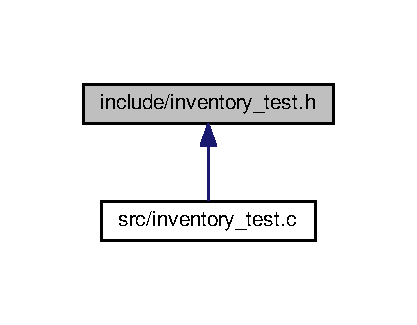
\includegraphics[width=200pt]{inventory__test_8h__dep__incl}
\end{center}
\end{figure}
\subsection*{Functions}
\begin{DoxyCompactItemize}
\item 
void \hyperlink{inventory__test_8h_a33638f1a88ae16ab8d6bee00145b82b8}{test1\+\_\+inventory\+\_\+create} ()
\item 
void \hyperlink{inventory__test_8h_a40a21fc4411716ecfa2bbb33c783df94}{test1\+\_\+inventory\+\_\+add\+\_\+id} ()
\item 
void \hyperlink{inventory__test_8h_abfb3407529398f76999549e42d567a7e}{test2\+\_\+inventory\+\_\+add\+\_\+id} ()
\item 
void \hyperlink{inventory__test_8h_adb75e7f71748feea51900c782343f550}{test3\+\_\+inventory\+\_\+add\+\_\+id} ()
\item 
void \hyperlink{inventory__test_8h_a967d37c163cbf8ea9335b506c1713f4a}{test4\+\_\+inventory\+\_\+add\+\_\+id} ()
\item 
void \hyperlink{inventory__test_8h_a8e69ae5a26b0115971e51ab94616fb85}{test5\+\_\+inventory\+\_\+add\+\_\+id} ()
\item 
void \hyperlink{inventory__test_8h_ac38fe4f7cdf9fa3972e975ee07caf876}{test1\+\_\+inventory\+\_\+get\+\_\+set} ()
\item 
void \hyperlink{inventory__test_8h_a66737b763a088f8a85549e846b01fbdb}{test2\+\_\+inventory\+\_\+get\+\_\+set} ()
\item 
void \hyperlink{inventory__test_8h_a30d80ddf084113e14192c7a5031528c5}{test1\+\_\+inventory\+\_\+delete\+\_\+id} ()
\item 
void \hyperlink{inventory__test_8h_a23c8b0ed664f86b5fdafbfbd875ee27d}{test2\+\_\+inventory\+\_\+delete\+\_\+id} ()
\item 
void \hyperlink{inventory__test_8h_a3dc930ea10c0e538e9f7227d5a7cdfa1}{test3\+\_\+inventory\+\_\+delete\+\_\+id} ()
\item 
void \hyperlink{inventory__test_8h_ab161eafe6a61db39b2237e97c677d822}{test1\+\_\+inventory\+\_\+destroy} ()
\item 
void \hyperlink{inventory__test_8h_a9f3daec28c696c0671e6a3e905359741}{test2\+\_\+inventory\+\_\+destroy} ()
\item 
void \hyperlink{inventory__test_8h_a7229ceb1916b0da955d23598da89d5ea}{test1\+\_\+inventory\+\_\+print} ()
\item 
void \hyperlink{inventory__test_8h_a7eb3ba387e33c42ff45331c9d9aada34}{test1\+\_\+inventory\+\_\+is\+\_\+full} ()
\item 
void \hyperlink{inventory__test_8h_a1c9e567d4919d5aaccc9580815a8a81d}{test2\+\_\+inventory\+\_\+is\+\_\+full} ()
\item 
void \hyperlink{inventory__test_8h_afe8c9730e30b58535afc0481970ab2b1}{test1\+\_\+inventory\+\_\+is\+\_\+empty} ()
\item 
void \hyperlink{inventory__test_8h_a4d2a2a4d4ba59446d013debfe9bf05dc}{test2\+\_\+inventory\+\_\+is\+\_\+empty} ()
\item 
void \hyperlink{inventory__test_8h_a9c8daeb141dbec6ddd5621edade53091}{test3\+\_\+inventory\+\_\+is\+\_\+empty} ()
\item 
void \hyperlink{inventory__test_8h_a76718582c0fbf43fbfc9e6bf3264f48e}{test1\+\_\+inventory\+\_\+get\+\_\+object} ()
\item 
void \hyperlink{inventory__test_8h_a6a440546c4b5335db5bb0e93688bf847}{test2\+\_\+inventory\+\_\+get\+\_\+object} ()
\end{DoxyCompactItemize}


\subsection{Detailed Description}
It declares the tests for the inventory module. 

\begin{DoxyAuthor}{Author}
Andres Mena 
\end{DoxyAuthor}
\begin{DoxyVersion}{Version}
2.\+0 
\end{DoxyVersion}
\begin{DoxyDate}{Date}
01-\/04-\/2018 
\end{DoxyDate}
\begin{DoxyCopyright}{Copyright}
G\+NU Public License 
\end{DoxyCopyright}


\subsection{Function Documentation}
\index{inventory\+\_\+test.\+h@{inventory\+\_\+test.\+h}!test1\+\_\+inventory\+\_\+add\+\_\+id@{test1\+\_\+inventory\+\_\+add\+\_\+id}}
\index{test1\+\_\+inventory\+\_\+add\+\_\+id@{test1\+\_\+inventory\+\_\+add\+\_\+id}!inventory\+\_\+test.\+h@{inventory\+\_\+test.\+h}}
\subsubsection[{\texorpdfstring{test1\+\_\+inventory\+\_\+add\+\_\+id()}{test1_inventory_add_id()}}]{\setlength{\rightskip}{0pt plus 5cm}void test1\+\_\+inventory\+\_\+add\+\_\+id (
\begin{DoxyParamCaption}
{}
\end{DoxyParamCaption}
)}\hypertarget{inventory__test_8h_a40a21fc4411716ecfa2bbb33c783df94}{}\label{inventory__test_8h_a40a21fc4411716ecfa2bbb33c783df94}
\begin{DoxyRefDesc}{Test}
\item[\hyperlink{test__test000002}{Test}]Test adding id to inventory \end{DoxyRefDesc}
\begin{DoxyPrecond}{Precondition}
N\+U\+LL pointer to inventory 
\end{DoxyPrecond}
\begin{DoxyPostcond}{Postcondition}
S\+T\+A\+T\+US == E\+R\+R\+OR 
\end{DoxyPostcond}
\index{inventory\+\_\+test.\+h@{inventory\+\_\+test.\+h}!test1\+\_\+inventory\+\_\+create@{test1\+\_\+inventory\+\_\+create}}
\index{test1\+\_\+inventory\+\_\+create@{test1\+\_\+inventory\+\_\+create}!inventory\+\_\+test.\+h@{inventory\+\_\+test.\+h}}
\subsubsection[{\texorpdfstring{test1\+\_\+inventory\+\_\+create()}{test1_inventory_create()}}]{\setlength{\rightskip}{0pt plus 5cm}void test1\+\_\+inventory\+\_\+create (
\begin{DoxyParamCaption}
{}
\end{DoxyParamCaption}
)}\hypertarget{inventory__test_8h_a33638f1a88ae16ab8d6bee00145b82b8}{}\label{inventory__test_8h_a33638f1a88ae16ab8d6bee00145b82b8}
\begin{DoxyRefDesc}{Test}
\item[\hyperlink{test__test000001}{Test}]Test inventory creation \end{DoxyRefDesc}
\begin{DoxyPrecond}{Precondition}
link ID 
\end{DoxyPrecond}
\begin{DoxyPostcond}{Postcondition}
Non N\+U\+LL pointer to inventory 
\end{DoxyPostcond}
\index{inventory\+\_\+test.\+h@{inventory\+\_\+test.\+h}!test1\+\_\+inventory\+\_\+delete\+\_\+id@{test1\+\_\+inventory\+\_\+delete\+\_\+id}}
\index{test1\+\_\+inventory\+\_\+delete\+\_\+id@{test1\+\_\+inventory\+\_\+delete\+\_\+id}!inventory\+\_\+test.\+h@{inventory\+\_\+test.\+h}}
\subsubsection[{\texorpdfstring{test1\+\_\+inventory\+\_\+delete\+\_\+id()}{test1_inventory_delete_id()}}]{\setlength{\rightskip}{0pt plus 5cm}void test1\+\_\+inventory\+\_\+delete\+\_\+id (
\begin{DoxyParamCaption}
{}
\end{DoxyParamCaption}
)}\hypertarget{inventory__test_8h_a30d80ddf084113e14192c7a5031528c5}{}\label{inventory__test_8h_a30d80ddf084113e14192c7a5031528c5}
\begin{DoxyRefDesc}{Test}
\item[\hyperlink{test__test000009}{Test}]Test deleting id from inventory \end{DoxyRefDesc}
\begin{DoxyPrecond}{Precondition}
N\+U\+LL pointer to inventory and N\+O\+\_\+\+ID 
\end{DoxyPrecond}
\begin{DoxyPostcond}{Postcondition}
E\+R\+R\+OR 
\end{DoxyPostcond}
\index{inventory\+\_\+test.\+h@{inventory\+\_\+test.\+h}!test1\+\_\+inventory\+\_\+destroy@{test1\+\_\+inventory\+\_\+destroy}}
\index{test1\+\_\+inventory\+\_\+destroy@{test1\+\_\+inventory\+\_\+destroy}!inventory\+\_\+test.\+h@{inventory\+\_\+test.\+h}}
\subsubsection[{\texorpdfstring{test1\+\_\+inventory\+\_\+destroy()}{test1_inventory_destroy()}}]{\setlength{\rightskip}{0pt plus 5cm}void test1\+\_\+inventory\+\_\+destroy (
\begin{DoxyParamCaption}
{}
\end{DoxyParamCaption}
)}\hypertarget{inventory__test_8h_ab161eafe6a61db39b2237e97c677d822}{}\label{inventory__test_8h_ab161eafe6a61db39b2237e97c677d822}
\begin{DoxyRefDesc}{Test}
\item[\hyperlink{test__test000012}{Test}]Test destroying inventory \end{DoxyRefDesc}
\begin{DoxyPrecond}{Precondition}
N\+U\+LL pointer to inventory 
\end{DoxyPrecond}
\begin{DoxyPostcond}{Postcondition}
E\+R\+R\+OR 
\end{DoxyPostcond}
\index{inventory\+\_\+test.\+h@{inventory\+\_\+test.\+h}!test1\+\_\+inventory\+\_\+get\+\_\+object@{test1\+\_\+inventory\+\_\+get\+\_\+object}}
\index{test1\+\_\+inventory\+\_\+get\+\_\+object@{test1\+\_\+inventory\+\_\+get\+\_\+object}!inventory\+\_\+test.\+h@{inventory\+\_\+test.\+h}}
\subsubsection[{\texorpdfstring{test1\+\_\+inventory\+\_\+get\+\_\+object()}{test1_inventory_get_object()}}]{\setlength{\rightskip}{0pt plus 5cm}void test1\+\_\+inventory\+\_\+get\+\_\+object (
\begin{DoxyParamCaption}
{}
\end{DoxyParamCaption}
)}\hypertarget{inventory__test_8h_a76718582c0fbf43fbfc9e6bf3264f48e}{}\label{inventory__test_8h_a76718582c0fbf43fbfc9e6bf3264f48e}
\begin{DoxyRefDesc}{Test}
\item[\hyperlink{test__test000020}{Test}]Test getting objects from inventory \end{DoxyRefDesc}
\begin{DoxyPrecond}{Precondition}
N\+U\+LL pointer to inventory 
\end{DoxyPrecond}
\begin{DoxyPostcond}{Postcondition}
N\+O\+\_\+\+ID 
\end{DoxyPostcond}
\index{inventory\+\_\+test.\+h@{inventory\+\_\+test.\+h}!test1\+\_\+inventory\+\_\+get\+\_\+set@{test1\+\_\+inventory\+\_\+get\+\_\+set}}
\index{test1\+\_\+inventory\+\_\+get\+\_\+set@{test1\+\_\+inventory\+\_\+get\+\_\+set}!inventory\+\_\+test.\+h@{inventory\+\_\+test.\+h}}
\subsubsection[{\texorpdfstring{test1\+\_\+inventory\+\_\+get\+\_\+set()}{test1_inventory_get_set()}}]{\setlength{\rightskip}{0pt plus 5cm}void test1\+\_\+inventory\+\_\+get\+\_\+set (
\begin{DoxyParamCaption}
{}
\end{DoxyParamCaption}
)}\hypertarget{inventory__test_8h_ac38fe4f7cdf9fa3972e975ee07caf876}{}\label{inventory__test_8h_ac38fe4f7cdf9fa3972e975ee07caf876}
\begin{DoxyRefDesc}{Test}
\item[\hyperlink{test__test000007}{Test}]Test getting set from inventory \end{DoxyRefDesc}
\begin{DoxyPrecond}{Precondition}
N\+U\+LL pointer to inventory 
\end{DoxyPrecond}
\begin{DoxyPostcond}{Postcondition}
N\+U\+LL set pointer 
\end{DoxyPostcond}
\index{inventory\+\_\+test.\+h@{inventory\+\_\+test.\+h}!test1\+\_\+inventory\+\_\+is\+\_\+empty@{test1\+\_\+inventory\+\_\+is\+\_\+empty}}
\index{test1\+\_\+inventory\+\_\+is\+\_\+empty@{test1\+\_\+inventory\+\_\+is\+\_\+empty}!inventory\+\_\+test.\+h@{inventory\+\_\+test.\+h}}
\subsubsection[{\texorpdfstring{test1\+\_\+inventory\+\_\+is\+\_\+empty()}{test1_inventory_is_empty()}}]{\setlength{\rightskip}{0pt plus 5cm}void test1\+\_\+inventory\+\_\+is\+\_\+empty (
\begin{DoxyParamCaption}
{}
\end{DoxyParamCaption}
)}\hypertarget{inventory__test_8h_afe8c9730e30b58535afc0481970ab2b1}{}\label{inventory__test_8h_afe8c9730e30b58535afc0481970ab2b1}
\begin{DoxyRefDesc}{Test}
\item[\hyperlink{test__test000017}{Test}]Test if inventory is empty \end{DoxyRefDesc}
\begin{DoxyPrecond}{Precondition}
N\+U\+LL Ponter to inventory 
\end{DoxyPrecond}
\begin{DoxyPostcond}{Postcondition}
B\+O\+OL == F\+A\+L\+SE 
\end{DoxyPostcond}
\index{inventory\+\_\+test.\+h@{inventory\+\_\+test.\+h}!test1\+\_\+inventory\+\_\+is\+\_\+full@{test1\+\_\+inventory\+\_\+is\+\_\+full}}
\index{test1\+\_\+inventory\+\_\+is\+\_\+full@{test1\+\_\+inventory\+\_\+is\+\_\+full}!inventory\+\_\+test.\+h@{inventory\+\_\+test.\+h}}
\subsubsection[{\texorpdfstring{test1\+\_\+inventory\+\_\+is\+\_\+full()}{test1_inventory_is_full()}}]{\setlength{\rightskip}{0pt plus 5cm}void test1\+\_\+inventory\+\_\+is\+\_\+full (
\begin{DoxyParamCaption}
{}
\end{DoxyParamCaption}
)}\hypertarget{inventory__test_8h_a7eb3ba387e33c42ff45331c9d9aada34}{}\label{inventory__test_8h_a7eb3ba387e33c42ff45331c9d9aada34}
\begin{DoxyRefDesc}{Test}
\item[\hyperlink{test__test000015}{Test}]Test if inventory is full \end{DoxyRefDesc}
\begin{DoxyPrecond}{Precondition}
N\+U\+LL pointer to inventory 
\end{DoxyPrecond}
\begin{DoxyPostcond}{Postcondition}
B\+O\+OL == F\+A\+L\+SE 
\end{DoxyPostcond}
\index{inventory\+\_\+test.\+h@{inventory\+\_\+test.\+h}!test1\+\_\+inventory\+\_\+print@{test1\+\_\+inventory\+\_\+print}}
\index{test1\+\_\+inventory\+\_\+print@{test1\+\_\+inventory\+\_\+print}!inventory\+\_\+test.\+h@{inventory\+\_\+test.\+h}}
\subsubsection[{\texorpdfstring{test1\+\_\+inventory\+\_\+print()}{test1_inventory_print()}}]{\setlength{\rightskip}{0pt plus 5cm}void test1\+\_\+inventory\+\_\+print (
\begin{DoxyParamCaption}
{}
\end{DoxyParamCaption}
)}\hypertarget{inventory__test_8h_a7229ceb1916b0da955d23598da89d5ea}{}\label{inventory__test_8h_a7229ceb1916b0da955d23598da89d5ea}
\begin{DoxyRefDesc}{Test}
\item[\hyperlink{test__test000014}{Test}]Test printing inventory \end{DoxyRefDesc}
\begin{DoxyPrecond}{Precondition}
N\+U\+LL pointer to inventory 
\end{DoxyPrecond}
\begin{DoxyPostcond}{Postcondition}
E\+R\+R\+OR 
\end{DoxyPostcond}
\index{inventory\+\_\+test.\+h@{inventory\+\_\+test.\+h}!test2\+\_\+inventory\+\_\+add\+\_\+id@{test2\+\_\+inventory\+\_\+add\+\_\+id}}
\index{test2\+\_\+inventory\+\_\+add\+\_\+id@{test2\+\_\+inventory\+\_\+add\+\_\+id}!inventory\+\_\+test.\+h@{inventory\+\_\+test.\+h}}
\subsubsection[{\texorpdfstring{test2\+\_\+inventory\+\_\+add\+\_\+id()}{test2_inventory_add_id()}}]{\setlength{\rightskip}{0pt plus 5cm}void test2\+\_\+inventory\+\_\+add\+\_\+id (
\begin{DoxyParamCaption}
{}
\end{DoxyParamCaption}
)}\hypertarget{inventory__test_8h_abfb3407529398f76999549e42d567a7e}{}\label{inventory__test_8h_abfb3407529398f76999549e42d567a7e}
\begin{DoxyRefDesc}{Test}
\item[\hyperlink{test__test000003}{Test}]Test adding id to inventory \end{DoxyRefDesc}
\begin{DoxyPrecond}{Precondition}
N\+U\+LL pointer to inventory and N\+O\+\_\+\+ID 
\end{DoxyPrecond}
\begin{DoxyPostcond}{Postcondition}
S\+T\+A\+T\+US == E\+R\+R\+OR 
\end{DoxyPostcond}
\index{inventory\+\_\+test.\+h@{inventory\+\_\+test.\+h}!test2\+\_\+inventory\+\_\+delete\+\_\+id@{test2\+\_\+inventory\+\_\+delete\+\_\+id}}
\index{test2\+\_\+inventory\+\_\+delete\+\_\+id@{test2\+\_\+inventory\+\_\+delete\+\_\+id}!inventory\+\_\+test.\+h@{inventory\+\_\+test.\+h}}
\subsubsection[{\texorpdfstring{test2\+\_\+inventory\+\_\+delete\+\_\+id()}{test2_inventory_delete_id()}}]{\setlength{\rightskip}{0pt plus 5cm}void test2\+\_\+inventory\+\_\+delete\+\_\+id (
\begin{DoxyParamCaption}
{}
\end{DoxyParamCaption}
)}\hypertarget{inventory__test_8h_a23c8b0ed664f86b5fdafbfbd875ee27d}{}\label{inventory__test_8h_a23c8b0ed664f86b5fdafbfbd875ee27d}
\begin{DoxyRefDesc}{Test}
\item[\hyperlink{test__test000010}{Test}]Test deleting id from inventory \end{DoxyRefDesc}
\begin{DoxyPrecond}{Precondition}
N\+U\+LL pointer to inventory and ID 
\end{DoxyPrecond}
\begin{DoxyPostcond}{Postcondition}
E\+R\+R\+OR 
\end{DoxyPostcond}
\index{inventory\+\_\+test.\+h@{inventory\+\_\+test.\+h}!test2\+\_\+inventory\+\_\+destroy@{test2\+\_\+inventory\+\_\+destroy}}
\index{test2\+\_\+inventory\+\_\+destroy@{test2\+\_\+inventory\+\_\+destroy}!inventory\+\_\+test.\+h@{inventory\+\_\+test.\+h}}
\subsubsection[{\texorpdfstring{test2\+\_\+inventory\+\_\+destroy()}{test2_inventory_destroy()}}]{\setlength{\rightskip}{0pt plus 5cm}void test2\+\_\+inventory\+\_\+destroy (
\begin{DoxyParamCaption}
{}
\end{DoxyParamCaption}
)}\hypertarget{inventory__test_8h_a9f3daec28c696c0671e6a3e905359741}{}\label{inventory__test_8h_a9f3daec28c696c0671e6a3e905359741}
\begin{DoxyRefDesc}{Test}
\item[\hyperlink{test__test000013}{Test}]Test destroying inventory \end{DoxyRefDesc}
\begin{DoxyPrecond}{Precondition}
Pointer to inventory 
\end{DoxyPrecond}
\begin{DoxyPostcond}{Postcondition}
OK 
\end{DoxyPostcond}
\index{inventory\+\_\+test.\+h@{inventory\+\_\+test.\+h}!test2\+\_\+inventory\+\_\+get\+\_\+object@{test2\+\_\+inventory\+\_\+get\+\_\+object}}
\index{test2\+\_\+inventory\+\_\+get\+\_\+object@{test2\+\_\+inventory\+\_\+get\+\_\+object}!inventory\+\_\+test.\+h@{inventory\+\_\+test.\+h}}
\subsubsection[{\texorpdfstring{test2\+\_\+inventory\+\_\+get\+\_\+object()}{test2_inventory_get_object()}}]{\setlength{\rightskip}{0pt plus 5cm}void test2\+\_\+inventory\+\_\+get\+\_\+object (
\begin{DoxyParamCaption}
{}
\end{DoxyParamCaption}
)}\hypertarget{inventory__test_8h_a6a440546c4b5335db5bb0e93688bf847}{}\label{inventory__test_8h_a6a440546c4b5335db5bb0e93688bf847}
\begin{DoxyRefDesc}{Test}
\item[\hyperlink{test__test000021}{Test}]Test getting objects from inventory \end{DoxyRefDesc}
\begin{DoxyPrecond}{Precondition}
Pointer to inventory with object 
\end{DoxyPrecond}
\begin{DoxyPostcond}{Postcondition}
id of object 
\end{DoxyPostcond}
\index{inventory\+\_\+test.\+h@{inventory\+\_\+test.\+h}!test2\+\_\+inventory\+\_\+get\+\_\+set@{test2\+\_\+inventory\+\_\+get\+\_\+set}}
\index{test2\+\_\+inventory\+\_\+get\+\_\+set@{test2\+\_\+inventory\+\_\+get\+\_\+set}!inventory\+\_\+test.\+h@{inventory\+\_\+test.\+h}}
\subsubsection[{\texorpdfstring{test2\+\_\+inventory\+\_\+get\+\_\+set()}{test2_inventory_get_set()}}]{\setlength{\rightskip}{0pt plus 5cm}void test2\+\_\+inventory\+\_\+get\+\_\+set (
\begin{DoxyParamCaption}
{}
\end{DoxyParamCaption}
)}\hypertarget{inventory__test_8h_a66737b763a088f8a85549e846b01fbdb}{}\label{inventory__test_8h_a66737b763a088f8a85549e846b01fbdb}
\begin{DoxyRefDesc}{Test}
\item[\hyperlink{test__test000008}{Test}]Test getting set from inventory \end{DoxyRefDesc}
\begin{DoxyPrecond}{Precondition}
Pointer to inventory 
\end{DoxyPrecond}
\begin{DoxyPostcond}{Postcondition}
non N\+U\+LL set pointer 
\end{DoxyPostcond}
\index{inventory\+\_\+test.\+h@{inventory\+\_\+test.\+h}!test2\+\_\+inventory\+\_\+is\+\_\+empty@{test2\+\_\+inventory\+\_\+is\+\_\+empty}}
\index{test2\+\_\+inventory\+\_\+is\+\_\+empty@{test2\+\_\+inventory\+\_\+is\+\_\+empty}!inventory\+\_\+test.\+h@{inventory\+\_\+test.\+h}}
\subsubsection[{\texorpdfstring{test2\+\_\+inventory\+\_\+is\+\_\+empty()}{test2_inventory_is_empty()}}]{\setlength{\rightskip}{0pt plus 5cm}void test2\+\_\+inventory\+\_\+is\+\_\+empty (
\begin{DoxyParamCaption}
{}
\end{DoxyParamCaption}
)}\hypertarget{inventory__test_8h_a4d2a2a4d4ba59446d013debfe9bf05dc}{}\label{inventory__test_8h_a4d2a2a4d4ba59446d013debfe9bf05dc}
\begin{DoxyRefDesc}{Test}
\item[\hyperlink{test__test000018}{Test}]Test if inventory is empty \end{DoxyRefDesc}
\begin{DoxyPrecond}{Precondition}
Ponter to inventory (with no objects) 
\end{DoxyPrecond}
\begin{DoxyPostcond}{Postcondition}
B\+O\+OL == F\+A\+L\+SE 
\end{DoxyPostcond}
\index{inventory\+\_\+test.\+h@{inventory\+\_\+test.\+h}!test2\+\_\+inventory\+\_\+is\+\_\+full@{test2\+\_\+inventory\+\_\+is\+\_\+full}}
\index{test2\+\_\+inventory\+\_\+is\+\_\+full@{test2\+\_\+inventory\+\_\+is\+\_\+full}!inventory\+\_\+test.\+h@{inventory\+\_\+test.\+h}}
\subsubsection[{\texorpdfstring{test2\+\_\+inventory\+\_\+is\+\_\+full()}{test2_inventory_is_full()}}]{\setlength{\rightskip}{0pt plus 5cm}void test2\+\_\+inventory\+\_\+is\+\_\+full (
\begin{DoxyParamCaption}
{}
\end{DoxyParamCaption}
)}\hypertarget{inventory__test_8h_a1c9e567d4919d5aaccc9580815a8a81d}{}\label{inventory__test_8h_a1c9e567d4919d5aaccc9580815a8a81d}
\begin{DoxyRefDesc}{Test}
\item[\hyperlink{test__test000016}{Test}]Test if inventory is full \end{DoxyRefDesc}
\begin{DoxyPrecond}{Precondition}
Ponter to inventory (not full) 
\end{DoxyPrecond}
\begin{DoxyPostcond}{Postcondition}
B\+O\+OL == F\+A\+L\+SE 
\end{DoxyPostcond}
\index{inventory\+\_\+test.\+h@{inventory\+\_\+test.\+h}!test3\+\_\+inventory\+\_\+add\+\_\+id@{test3\+\_\+inventory\+\_\+add\+\_\+id}}
\index{test3\+\_\+inventory\+\_\+add\+\_\+id@{test3\+\_\+inventory\+\_\+add\+\_\+id}!inventory\+\_\+test.\+h@{inventory\+\_\+test.\+h}}
\subsubsection[{\texorpdfstring{test3\+\_\+inventory\+\_\+add\+\_\+id()}{test3_inventory_add_id()}}]{\setlength{\rightskip}{0pt plus 5cm}void test3\+\_\+inventory\+\_\+add\+\_\+id (
\begin{DoxyParamCaption}
{}
\end{DoxyParamCaption}
)}\hypertarget{inventory__test_8h_adb75e7f71748feea51900c782343f550}{}\label{inventory__test_8h_adb75e7f71748feea51900c782343f550}
\begin{DoxyRefDesc}{Test}
\item[\hyperlink{test__test000004}{Test}]Test adding id to inventory \end{DoxyRefDesc}
\begin{DoxyPrecond}{Precondition}
Pointer to inventory and N\+O\+\_\+\+ID 
\end{DoxyPrecond}
\begin{DoxyPostcond}{Postcondition}
S\+T\+A\+T\+US == E\+R\+R\+OR 
\end{DoxyPostcond}
\index{inventory\+\_\+test.\+h@{inventory\+\_\+test.\+h}!test3\+\_\+inventory\+\_\+delete\+\_\+id@{test3\+\_\+inventory\+\_\+delete\+\_\+id}}
\index{test3\+\_\+inventory\+\_\+delete\+\_\+id@{test3\+\_\+inventory\+\_\+delete\+\_\+id}!inventory\+\_\+test.\+h@{inventory\+\_\+test.\+h}}
\subsubsection[{\texorpdfstring{test3\+\_\+inventory\+\_\+delete\+\_\+id()}{test3_inventory_delete_id()}}]{\setlength{\rightskip}{0pt plus 5cm}void test3\+\_\+inventory\+\_\+delete\+\_\+id (
\begin{DoxyParamCaption}
{}
\end{DoxyParamCaption}
)}\hypertarget{inventory__test_8h_a3dc930ea10c0e538e9f7227d5a7cdfa1}{}\label{inventory__test_8h_a3dc930ea10c0e538e9f7227d5a7cdfa1}
\begin{DoxyRefDesc}{Test}
\item[\hyperlink{test__test000011}{Test}]Test deleting id from inventory \end{DoxyRefDesc}
\begin{DoxyPrecond}{Precondition}
Pointer to inventory and id 
\end{DoxyPrecond}
\begin{DoxyPostcond}{Postcondition}
OK 
\end{DoxyPostcond}
\index{inventory\+\_\+test.\+h@{inventory\+\_\+test.\+h}!test3\+\_\+inventory\+\_\+is\+\_\+empty@{test3\+\_\+inventory\+\_\+is\+\_\+empty}}
\index{test3\+\_\+inventory\+\_\+is\+\_\+empty@{test3\+\_\+inventory\+\_\+is\+\_\+empty}!inventory\+\_\+test.\+h@{inventory\+\_\+test.\+h}}
\subsubsection[{\texorpdfstring{test3\+\_\+inventory\+\_\+is\+\_\+empty()}{test3_inventory_is_empty()}}]{\setlength{\rightskip}{0pt plus 5cm}void test3\+\_\+inventory\+\_\+is\+\_\+empty (
\begin{DoxyParamCaption}
{}
\end{DoxyParamCaption}
)}\hypertarget{inventory__test_8h_a9c8daeb141dbec6ddd5621edade53091}{}\label{inventory__test_8h_a9c8daeb141dbec6ddd5621edade53091}
\begin{DoxyRefDesc}{Test}
\item[\hyperlink{test__test000019}{Test}]Test if inventory is empty \end{DoxyRefDesc}
\begin{DoxyPrecond}{Precondition}
Ponter to inventory (with objects) 
\end{DoxyPrecond}
\begin{DoxyPostcond}{Postcondition}
B\+O\+OL == T\+R\+UE 
\end{DoxyPostcond}
\index{inventory\+\_\+test.\+h@{inventory\+\_\+test.\+h}!test4\+\_\+inventory\+\_\+add\+\_\+id@{test4\+\_\+inventory\+\_\+add\+\_\+id}}
\index{test4\+\_\+inventory\+\_\+add\+\_\+id@{test4\+\_\+inventory\+\_\+add\+\_\+id}!inventory\+\_\+test.\+h@{inventory\+\_\+test.\+h}}
\subsubsection[{\texorpdfstring{test4\+\_\+inventory\+\_\+add\+\_\+id()}{test4_inventory_add_id()}}]{\setlength{\rightskip}{0pt plus 5cm}void test4\+\_\+inventory\+\_\+add\+\_\+id (
\begin{DoxyParamCaption}
{}
\end{DoxyParamCaption}
)}\hypertarget{inventory__test_8h_a967d37c163cbf8ea9335b506c1713f4a}{}\label{inventory__test_8h_a967d37c163cbf8ea9335b506c1713f4a}
\begin{DoxyRefDesc}{Test}
\item[\hyperlink{test__test000005}{Test}]Test adding id to inventory \end{DoxyRefDesc}
\begin{DoxyPrecond}{Precondition}
Pointer to inventory and ID 
\end{DoxyPrecond}
\begin{DoxyPostcond}{Postcondition}
S\+T\+A\+T\+US == OK 
\end{DoxyPostcond}
\index{inventory\+\_\+test.\+h@{inventory\+\_\+test.\+h}!test5\+\_\+inventory\+\_\+add\+\_\+id@{test5\+\_\+inventory\+\_\+add\+\_\+id}}
\index{test5\+\_\+inventory\+\_\+add\+\_\+id@{test5\+\_\+inventory\+\_\+add\+\_\+id}!inventory\+\_\+test.\+h@{inventory\+\_\+test.\+h}}
\subsubsection[{\texorpdfstring{test5\+\_\+inventory\+\_\+add\+\_\+id()}{test5_inventory_add_id()}}]{\setlength{\rightskip}{0pt plus 5cm}void test5\+\_\+inventory\+\_\+add\+\_\+id (
\begin{DoxyParamCaption}
{}
\end{DoxyParamCaption}
)}\hypertarget{inventory__test_8h_a8e69ae5a26b0115971e51ab94616fb85}{}\label{inventory__test_8h_a8e69ae5a26b0115971e51ab94616fb85}
\begin{DoxyRefDesc}{Test}
\item[\hyperlink{test__test000006}{Test}]Test adding id to inventory \end{DoxyRefDesc}
\begin{DoxyPrecond}{Precondition}
Pointer to inventory and ID (full inventory) 
\end{DoxyPrecond}
\begin{DoxyPostcond}{Postcondition}
S\+T\+A\+T\+US == E\+R\+R\+OR 
\end{DoxyPostcond}

\hypertarget{link_8h}{}\section{include/link.h File Reference}
\label{link_8h}\index{include/link.\+h@{include/link.\+h}}


links spaces  


{\ttfamily \#include $<$stdio.\+h$>$}\\*
{\ttfamily \#include \char`\"{}types.\+h\char`\"{}}\\*
Include dependency graph for link.\+h\+:
\nopagebreak
\begin{figure}[H]
\begin{center}
\leavevmode
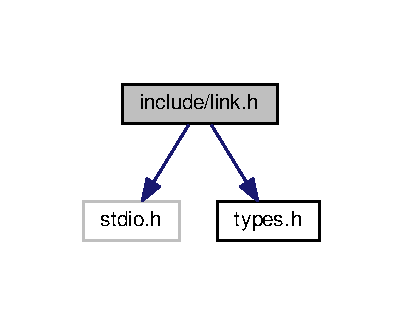
\includegraphics[width=194pt]{link_8h__incl}
\end{center}
\end{figure}
This graph shows which files directly or indirectly include this file\+:
\nopagebreak
\begin{figure}[H]
\begin{center}
\leavevmode
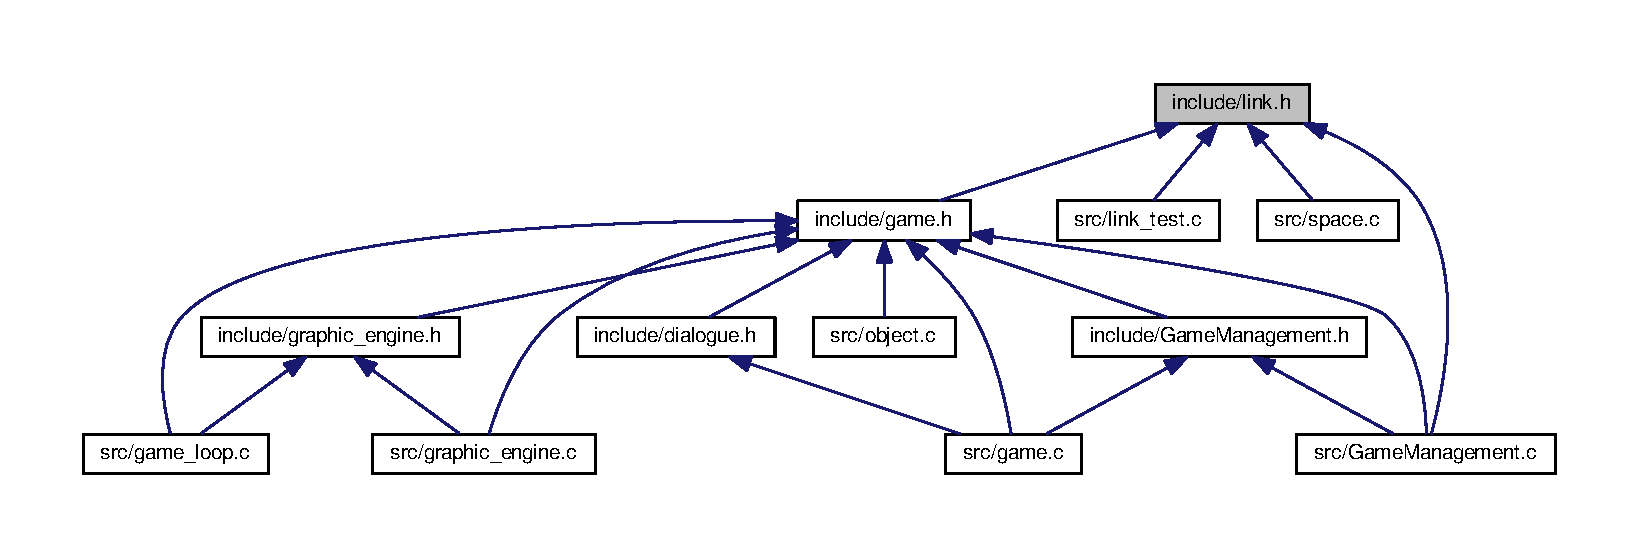
\includegraphics[width=350pt]{link_8h__dep__incl}
\end{center}
\end{figure}
\subsection*{Typedefs}
\begin{DoxyCompactItemize}
\item 
typedef struct \hyperlink{struct__Link}{\+\_\+\+Link} \hyperlink{link_8h_ae3b299941e67be6971bfd64a25505eff}{Link}
\begin{DoxyCompactList}\small\item\em link definition \end{DoxyCompactList}\end{DoxyCompactItemize}
\subsection*{Functions}
\begin{DoxyCompactItemize}
\item 
\hyperlink{link_8h_ae3b299941e67be6971bfd64a25505eff}{Link} $\ast$ \hyperlink{link_8h_a8090d7f529cfd6a2fc5df3dd379fe514}{link\+\_\+create} (\hyperlink{types_8h_a845e604fb28f7e3d97549da3448149d3}{Id} id)
\begin{DoxyCompactList}\small\item\em creates a link \end{DoxyCompactList}\item 
\hyperlink{types_8h_a32c27cc471df37f4fc818d65de0a56c4}{S\+T\+A\+T\+US} \hyperlink{link_8h_a85c4dd77887bf31f651ea1162144d712}{link\+\_\+destroy} (\hyperlink{link_8h_ae3b299941e67be6971bfd64a25505eff}{Link} $\ast$link)
\begin{DoxyCompactList}\small\item\em frees memory \end{DoxyCompactList}\item 
\hyperlink{types_8h_a32c27cc471df37f4fc818d65de0a56c4}{S\+T\+A\+T\+US} \hyperlink{link_8h_a3fd49fb1a3f19be4fc800ff07820cafb}{link\+\_\+set\+\_\+id} (\hyperlink{link_8h_ae3b299941e67be6971bfd64a25505eff}{Link} $\ast$link, \hyperlink{types_8h_a845e604fb28f7e3d97549da3448149d3}{Id} id)
\begin{DoxyCompactList}\small\item\em sets an id \end{DoxyCompactList}\item 
\hyperlink{types_8h_a32c27cc471df37f4fc818d65de0a56c4}{S\+T\+A\+T\+US} \hyperlink{link_8h_a6c7a3bd7a856288c377edbcd045912e6}{link\+\_\+set\+\_\+name} (\hyperlink{link_8h_ae3b299941e67be6971bfd64a25505eff}{Link} $\ast$link, char $\ast$name)
\begin{DoxyCompactList}\small\item\em sets a name \end{DoxyCompactList}\item 
\hyperlink{types_8h_a32c27cc471df37f4fc818d65de0a56c4}{S\+T\+A\+T\+US} \hyperlink{link_8h_a526a62eef81c93938b7e8ee4a754c63c}{link\+\_\+set\+\_\+link1} (\hyperlink{link_8h_ae3b299941e67be6971bfd64a25505eff}{Link} $\ast$link, \hyperlink{types_8h_a845e604fb28f7e3d97549da3448149d3}{Id} id)
\begin{DoxyCompactList}\small\item\em sets link number one \end{DoxyCompactList}\item 
\hyperlink{types_8h_a32c27cc471df37f4fc818d65de0a56c4}{S\+T\+A\+T\+US} \hyperlink{link_8h_a5e595d652382a65538d7017b82774d42}{link\+\_\+set\+\_\+link2} (\hyperlink{link_8h_ae3b299941e67be6971bfd64a25505eff}{Link} $\ast$link, \hyperlink{types_8h_a845e604fb28f7e3d97549da3448149d3}{Id} id)
\begin{DoxyCompactList}\small\item\em sets link number two \end{DoxyCompactList}\item 
\hyperlink{types_8h_a32c27cc471df37f4fc818d65de0a56c4}{S\+T\+A\+T\+US} \hyperlink{link_8h_a172c8b5a328c0451c74647439c74a60d}{link\+\_\+set\+\_\+status} (\hyperlink{link_8h_ae3b299941e67be6971bfd64a25505eff}{Link} $\ast$link, \hyperlink{types_8h_a3425906c2a1ce4f324e3b2006ece02cd}{L\+I\+N\+K\+\_\+\+ST} st)
\begin{DoxyCompactList}\small\item\em sets the status of the link \end{DoxyCompactList}\item 
\hyperlink{types_8h_a845e604fb28f7e3d97549da3448149d3}{Id} \hyperlink{link_8h_a2bbd320f995a72b2ea7ea639b1c81892}{link\+\_\+get\+\_\+id} (\hyperlink{link_8h_ae3b299941e67be6971bfd64a25505eff}{Link} $\ast$link)
\begin{DoxyCompactList}\small\item\em gets id of the link \end{DoxyCompactList}\item 
\hyperlink{types_8h_a845e604fb28f7e3d97549da3448149d3}{Id} \hyperlink{link_8h_a5ab57cf8161d09e8cda55c234d22ab66}{link\+\_\+get\+\_\+link1} (\hyperlink{link_8h_ae3b299941e67be6971bfd64a25505eff}{Link} $\ast$link)
\begin{DoxyCompactList}\small\item\em gets id of the link number one \end{DoxyCompactList}\item 
\hyperlink{types_8h_a845e604fb28f7e3d97549da3448149d3}{Id} \hyperlink{link_8h_ad274fe544465f3684d22b2a4dfa2c0bd}{link\+\_\+get\+\_\+link2} (\hyperlink{link_8h_ae3b299941e67be6971bfd64a25505eff}{Link} $\ast$link)
\begin{DoxyCompactList}\small\item\em gets id of the link number two \end{DoxyCompactList}\item 
const char $\ast$ \hyperlink{link_8h_aaab4c9c7d5492873cafd9e11dc0f8059}{link\+\_\+get\+\_\+name} (\hyperlink{link_8h_ae3b299941e67be6971bfd64a25505eff}{Link} $\ast$link)
\begin{DoxyCompactList}\small\item\em gets name of the link \end{DoxyCompactList}\item 
\hyperlink{types_8h_a3425906c2a1ce4f324e3b2006ece02cd}{L\+I\+N\+K\+\_\+\+ST} \hyperlink{link_8h_a477b0cf9e85264be7ef7e41d69ff2154}{link\+\_\+get\+\_\+status} (\hyperlink{link_8h_ae3b299941e67be6971bfd64a25505eff}{Link} $\ast$link)
\begin{DoxyCompactList}\small\item\em gets the status of the link \end{DoxyCompactList}\item 
\hyperlink{types_8h_a32c27cc471df37f4fc818d65de0a56c4}{S\+T\+A\+T\+US} \hyperlink{link_8h_a95ea756dad592e65440a33dfbe47edcf}{link\+\_\+print} (\hyperlink{link_8h_ae3b299941e67be6971bfd64a25505eff}{Link} $\ast$link)
\begin{DoxyCompactList}\small\item\em prints links \end{DoxyCompactList}\item 
\hyperlink{types_8h_a845e604fb28f7e3d97549da3448149d3}{Id} \hyperlink{link_8h_ad064a2ab07b42a46988ae27c57bfc0b6}{link\+\_\+get\+\_\+key} (\hyperlink{link_8h_ae3b299941e67be6971bfd64a25505eff}{Link} $\ast$link)
\begin{DoxyCompactList}\small\item\em gets key to open link \end{DoxyCompactList}\item 
\hyperlink{types_8h_a32c27cc471df37f4fc818d65de0a56c4}{S\+T\+A\+T\+US} \hyperlink{link_8h_a394f1e4bd521e02c72a6473f14bab609}{link\+\_\+set\+\_\+key} (\hyperlink{link_8h_ae3b299941e67be6971bfd64a25505eff}{Link} $\ast$link, \hyperlink{types_8h_a845e604fb28f7e3d97549da3448149d3}{Id} key)
\begin{DoxyCompactList}\small\item\em sets key to open link \end{DoxyCompactList}\end{DoxyCompactItemize}


\subsection{Detailed Description}
links spaces 

Module that links the spaces of the game by putting together the ones who are\+: \char`\"{}death\char`\"{}, \char`\"{}goose\char`\"{} and \char`\"{}bridge\char`\"{}. It also links spaces which distance is one space between them.

\begin{DoxyAuthor}{Author}
Andrés Mena 
\end{DoxyAuthor}
\begin{DoxyVersion}{Version}
1.\+1 
\end{DoxyVersion}
\begin{DoxyDate}{Date}
07-\/04-\/2018 
\end{DoxyDate}


\subsection{Typedef Documentation}
\index{link.\+h@{link.\+h}!Link@{Link}}
\index{Link@{Link}!link.\+h@{link.\+h}}
\subsubsection[{\texorpdfstring{Link}{Link}}]{\setlength{\rightskip}{0pt plus 5cm}typedef struct {\bf \+\_\+\+Link} {\bf Link}}\hypertarget{link_8h_ae3b299941e67be6971bfd64a25505eff}{}\label{link_8h_ae3b299941e67be6971bfd64a25505eff}


link definition 

Struct for storing a link with its properties. 

\subsection{Function Documentation}
\index{link.\+h@{link.\+h}!link\+\_\+create@{link\+\_\+create}}
\index{link\+\_\+create@{link\+\_\+create}!link.\+h@{link.\+h}}
\subsubsection[{\texorpdfstring{link\+\_\+create(\+Id id)}{link_create(Id id)}}]{\setlength{\rightskip}{0pt plus 5cm}{\bf Link}$\ast$ link\+\_\+create (
\begin{DoxyParamCaption}
\item[{{\bf Id}}]{id}
\end{DoxyParamCaption}
)}\hypertarget{link_8h_a8090d7f529cfd6a2fc5df3dd379fe514}{}\label{link_8h_a8090d7f529cfd6a2fc5df3dd379fe514}


creates a link 

It creates a new link, if id is -\/1(N\+O\+\_\+\+ID), N\+U\+LL is returned, if not, memory for a new link is reserved and created. If anything goes wrong, it returns N\+U\+LL.

\begin{DoxyAuthor}{Author}
Andrés Mena 
\end{DoxyAuthor}

\begin{DoxyParams}{Parameters}
{\em id} & long int. \\
\hline
\end{DoxyParams}
\begin{DoxyReturn}{Returns}
pointer to link, N\+U\+LL if something goes wrong. 
\end{DoxyReturn}
\index{link.\+h@{link.\+h}!link\+\_\+destroy@{link\+\_\+destroy}}
\index{link\+\_\+destroy@{link\+\_\+destroy}!link.\+h@{link.\+h}}
\subsubsection[{\texorpdfstring{link\+\_\+destroy(\+Link $\ast$link)}{link_destroy(Link *link)}}]{\setlength{\rightskip}{0pt plus 5cm}{\bf S\+T\+A\+T\+US} link\+\_\+destroy (
\begin{DoxyParamCaption}
\item[{{\bf Link} $\ast$}]{link}
\end{DoxyParamCaption}
)}\hypertarget{link_8h_a85c4dd77887bf31f651ea1162144d712}{}\label{link_8h_a85c4dd77887bf31f651ea1162144d712}


frees memory 

Receives pointer to link and frees the memory it occupied.

\begin{DoxyAuthor}{Author}
Andrés Mena 
\end{DoxyAuthor}

\begin{DoxyParams}{Parameters}
{\em link} & pointer to link. \\
\hline
\end{DoxyParams}
\begin{DoxyReturn}{Returns}
S\+T\+A\+T\+US, E\+R\+R\+OR if argument received is N\+U\+LL, if not, OK. 
\end{DoxyReturn}
\index{link.\+h@{link.\+h}!link\+\_\+get\+\_\+id@{link\+\_\+get\+\_\+id}}
\index{link\+\_\+get\+\_\+id@{link\+\_\+get\+\_\+id}!link.\+h@{link.\+h}}
\subsubsection[{\texorpdfstring{link\+\_\+get\+\_\+id(\+Link $\ast$link)}{link_get_id(Link *link)}}]{\setlength{\rightskip}{0pt plus 5cm}{\bf Id} link\+\_\+get\+\_\+id (
\begin{DoxyParamCaption}
\item[{{\bf Link} $\ast$}]{link}
\end{DoxyParamCaption}
)}\hypertarget{link_8h_a2bbd320f995a72b2ea7ea639b1c81892}{}\label{link_8h_a2bbd320f995a72b2ea7ea639b1c81892}


gets id of the link 

Returns the id of the link, if ID = N\+O\+\_\+\+ID(-\/1), gives E\+R\+R\+OR and returns N\+O\+\_\+\+ID.

\begin{DoxyAuthor}{Author}
Andrés Mena 
\end{DoxyAuthor}

\begin{DoxyParams}{Parameters}
{\em link} & pointer to link. \\
\hline
\end{DoxyParams}
\begin{DoxyReturn}{Returns}
Id, N\+O\+\_\+\+ID if link is pointing N\+U\+LL. 
\end{DoxyReturn}
\index{link.\+h@{link.\+h}!link\+\_\+get\+\_\+key@{link\+\_\+get\+\_\+key}}
\index{link\+\_\+get\+\_\+key@{link\+\_\+get\+\_\+key}!link.\+h@{link.\+h}}
\subsubsection[{\texorpdfstring{link\+\_\+get\+\_\+key(\+Link $\ast$link)}{link_get_key(Link *link)}}]{\setlength{\rightskip}{0pt plus 5cm}{\bf Id} link\+\_\+get\+\_\+key (
\begin{DoxyParamCaption}
\item[{{\bf Link} $\ast$}]{link}
\end{DoxyParamCaption}
)}\hypertarget{link_8h_ad064a2ab07b42a46988ae27c57bfc0b6}{}\label{link_8h_ad064a2ab07b42a46988ae27c57bfc0b6}


gets key to open link 

Function in charge of returning the key that is used to open a link.

\begin{DoxyAuthor}{Author}
Andrés Mena 
\end{DoxyAuthor}

\begin{DoxyParams}{Parameters}
{\em link} & pointer to link. \\
\hline
\end{DoxyParams}
\begin{DoxyReturn}{Returns}
Id, N\+O\+\_\+\+ID if object is pointing N\+U\+LL. 
\end{DoxyReturn}
\index{link.\+h@{link.\+h}!link\+\_\+get\+\_\+link1@{link\+\_\+get\+\_\+link1}}
\index{link\+\_\+get\+\_\+link1@{link\+\_\+get\+\_\+link1}!link.\+h@{link.\+h}}
\subsubsection[{\texorpdfstring{link\+\_\+get\+\_\+link1(\+Link $\ast$link)}{link_get_link1(Link *link)}}]{\setlength{\rightskip}{0pt plus 5cm}{\bf Id} link\+\_\+get\+\_\+link1 (
\begin{DoxyParamCaption}
\item[{{\bf Link} $\ast$}]{link}
\end{DoxyParamCaption}
)}\hypertarget{link_8h_a5ab57cf8161d09e8cda55c234d22ab66}{}\label{link_8h_a5ab57cf8161d09e8cda55c234d22ab66}


gets id of the link number one 

Returns the id of the link number one compared, if ID = N\+O\+\_\+\+ID(-\/1), gives E\+R\+R\+OR and returns N\+O\+\_\+\+ID.

\begin{DoxyAuthor}{Author}
Andrés Mena 
\end{DoxyAuthor}

\begin{DoxyParams}{Parameters}
{\em link} & pointer to link. \\
\hline
\end{DoxyParams}
\begin{DoxyReturn}{Returns}
Id, N\+O\+\_\+\+ID if link is pointing N\+U\+LL. 
\end{DoxyReturn}
\index{link.\+h@{link.\+h}!link\+\_\+get\+\_\+link2@{link\+\_\+get\+\_\+link2}}
\index{link\+\_\+get\+\_\+link2@{link\+\_\+get\+\_\+link2}!link.\+h@{link.\+h}}
\subsubsection[{\texorpdfstring{link\+\_\+get\+\_\+link2(\+Link $\ast$link)}{link_get_link2(Link *link)}}]{\setlength{\rightskip}{0pt plus 5cm}{\bf Id} link\+\_\+get\+\_\+link2 (
\begin{DoxyParamCaption}
\item[{{\bf Link} $\ast$}]{link}
\end{DoxyParamCaption}
)}\hypertarget{link_8h_ad274fe544465f3684d22b2a4dfa2c0bd}{}\label{link_8h_ad274fe544465f3684d22b2a4dfa2c0bd}


gets id of the link number two 

Returns the id of the link number two, if ID = N\+O\+\_\+\+ID(-\/1), gives E\+R\+R\+OR and returns N\+O\+\_\+\+ID.

\begin{DoxyAuthor}{Author}
Andrés Mena 
\end{DoxyAuthor}

\begin{DoxyParams}{Parameters}
{\em link} & pointer to link. \\
\hline
\end{DoxyParams}
\begin{DoxyReturn}{Returns}
Id, N\+O\+\_\+\+ID if link is pointing N\+U\+LL. 
\end{DoxyReturn}
\index{link.\+h@{link.\+h}!link\+\_\+get\+\_\+name@{link\+\_\+get\+\_\+name}}
\index{link\+\_\+get\+\_\+name@{link\+\_\+get\+\_\+name}!link.\+h@{link.\+h}}
\subsubsection[{\texorpdfstring{link\+\_\+get\+\_\+name(\+Link $\ast$link)}{link_get_name(Link *link)}}]{\setlength{\rightskip}{0pt plus 5cm}const char$\ast$ link\+\_\+get\+\_\+name (
\begin{DoxyParamCaption}
\item[{{\bf Link} $\ast$}]{link}
\end{DoxyParamCaption}
)}\hypertarget{link_8h_aaab4c9c7d5492873cafd9e11dc0f8059}{}\label{link_8h_aaab4c9c7d5492873cafd9e11dc0f8059}


gets name of the link 

Returns a constant string of characters which will be the name of the link.

\begin{DoxyAuthor}{Author}
Andrés Mena 
\end{DoxyAuthor}

\begin{DoxyParams}{Parameters}
{\em link} & pointer to link. \\
\hline
\end{DoxyParams}
\begin{DoxyReturn}{Returns}
constant string of characters. 
\end{DoxyReturn}
\index{link.\+h@{link.\+h}!link\+\_\+get\+\_\+status@{link\+\_\+get\+\_\+status}}
\index{link\+\_\+get\+\_\+status@{link\+\_\+get\+\_\+status}!link.\+h@{link.\+h}}
\subsubsection[{\texorpdfstring{link\+\_\+get\+\_\+status(\+Link $\ast$link)}{link_get_status(Link *link)}}]{\setlength{\rightskip}{0pt plus 5cm}{\bf L\+I\+N\+K\+\_\+\+ST} link\+\_\+get\+\_\+status (
\begin{DoxyParamCaption}
\item[{{\bf Link} $\ast$}]{link}
\end{DoxyParamCaption}
)}\hypertarget{link_8h_a477b0cf9e85264be7ef7e41d69ff2154}{}\label{link_8h_a477b0cf9e85264be7ef7e41d69ff2154}


gets the status of the link 

If there is an error, C\+L\+O\+SE is returned, normally it will return the O\+P\+EN status because it will be working properly.

\begin{DoxyAuthor}{Author}
Andrés Mena 
\end{DoxyAuthor}

\begin{DoxyParams}{Parameters}
{\em link} & pointer to link. \\
\hline
\end{DoxyParams}
\begin{DoxyReturn}{Returns}
L\+I\+NK S\+T\+A\+T\+US, C\+L\+O\+SE if argument received is N\+U\+LL, if not, O\+P\+EN. 
\end{DoxyReturn}
\index{link.\+h@{link.\+h}!link\+\_\+print@{link\+\_\+print}}
\index{link\+\_\+print@{link\+\_\+print}!link.\+h@{link.\+h}}
\subsubsection[{\texorpdfstring{link\+\_\+print(\+Link $\ast$link)}{link_print(Link *link)}}]{\setlength{\rightskip}{0pt plus 5cm}{\bf S\+T\+A\+T\+US} link\+\_\+print (
\begin{DoxyParamCaption}
\item[{{\bf Link} $\ast$}]{link}
\end{DoxyParamCaption}
)}\hypertarget{link_8h_a95ea756dad592e65440a33dfbe47edcf}{}\label{link_8h_a95ea756dad592e65440a33dfbe47edcf}


prints links 

Function in charge of printing the link, in order to check that everything is working correctly by calling some of its functions.

\begin{DoxyAuthor}{Author}
Andrés Mena 
\end{DoxyAuthor}

\begin{DoxyParams}{Parameters}
{\em link} & pointer to link. \\
\hline
\end{DoxyParams}
\begin{DoxyReturn}{Returns}
S\+T\+A\+T\+US, E\+R\+R\+OR if argument received is N\+U\+LL, if not, OK. 
\end{DoxyReturn}
\index{link.\+h@{link.\+h}!link\+\_\+set\+\_\+id@{link\+\_\+set\+\_\+id}}
\index{link\+\_\+set\+\_\+id@{link\+\_\+set\+\_\+id}!link.\+h@{link.\+h}}
\subsubsection[{\texorpdfstring{link\+\_\+set\+\_\+id(\+Link $\ast$link, Id id)}{link_set_id(Link *link, Id id)}}]{\setlength{\rightskip}{0pt plus 5cm}{\bf S\+T\+A\+T\+US} link\+\_\+set\+\_\+id (
\begin{DoxyParamCaption}
\item[{{\bf Link} $\ast$}]{link, }
\item[{{\bf Id}}]{id}
\end{DoxyParamCaption}
)}\hypertarget{link_8h_a3fd49fb1a3f19be4fc800ff07820cafb}{}\label{link_8h_a3fd49fb1a3f19be4fc800ff07820cafb}


sets an id 

If there is an error, E\+R\+R\+OR is returned, if not, it establishes an id for the link.

\begin{DoxyAuthor}{Author}
Andrés Mena 
\end{DoxyAuthor}

\begin{DoxyParams}{Parameters}
{\em link} & pointer to link. \\
\hline
{\em id} & long int. \\
\hline
\end{DoxyParams}
\begin{DoxyReturn}{Returns}
S\+T\+A\+T\+US, E\+R\+R\+OR if argument received is N\+U\+LL, if not, OK. 
\end{DoxyReturn}
\index{link.\+h@{link.\+h}!link\+\_\+set\+\_\+key@{link\+\_\+set\+\_\+key}}
\index{link\+\_\+set\+\_\+key@{link\+\_\+set\+\_\+key}!link.\+h@{link.\+h}}
\subsubsection[{\texorpdfstring{link\+\_\+set\+\_\+key(\+Link $\ast$link, Id key)}{link_set_key(Link *link, Id key)}}]{\setlength{\rightskip}{0pt plus 5cm}{\bf S\+T\+A\+T\+US} link\+\_\+set\+\_\+key (
\begin{DoxyParamCaption}
\item[{{\bf Link} $\ast$}]{link, }
\item[{{\bf Id}}]{key}
\end{DoxyParamCaption}
)}\hypertarget{link_8h_a394f1e4bd521e02c72a6473f14bab609}{}\label{link_8h_a394f1e4bd521e02c72a6473f14bab609}


sets key to open link 

Function that it is used to set a link to the key that enables us to open that link with the key.

\begin{DoxyAuthor}{Author}
Andrés Mena 
\end{DoxyAuthor}

\begin{DoxyParams}{Parameters}
{\em link} & pointer to link. \\
\hline
{\em key} & long int. \\
\hline
\end{DoxyParams}
\begin{DoxyReturn}{Returns}
S\+T\+A\+T\+US, E\+R\+R\+OR if argument received is N\+U\+LL, if not, OK. 
\end{DoxyReturn}
\index{link.\+h@{link.\+h}!link\+\_\+set\+\_\+link1@{link\+\_\+set\+\_\+link1}}
\index{link\+\_\+set\+\_\+link1@{link\+\_\+set\+\_\+link1}!link.\+h@{link.\+h}}
\subsubsection[{\texorpdfstring{link\+\_\+set\+\_\+link1(\+Link $\ast$link, Id id)}{link_set_link1(Link *link, Id id)}}]{\setlength{\rightskip}{0pt plus 5cm}{\bf S\+T\+A\+T\+US} link\+\_\+set\+\_\+link1 (
\begin{DoxyParamCaption}
\item[{{\bf Link} $\ast$}]{link, }
\item[{{\bf Id}}]{id}
\end{DoxyParamCaption}
)}\hypertarget{link_8h_a526a62eef81c93938b7e8ee4a754c63c}{}\label{link_8h_a526a62eef81c93938b7e8ee4a754c63c}


sets link number one 

If there is an error, E\+R\+R\+OR is returned, if not, it gives an id to the first link compared.

\begin{DoxyAuthor}{Author}
Andrés Mena 
\end{DoxyAuthor}

\begin{DoxyParams}{Parameters}
{\em link} & pointer to link. \\
\hline
{\em id} & long int. \\
\hline
\end{DoxyParams}
\begin{DoxyReturn}{Returns}
S\+T\+A\+T\+US, E\+R\+R\+OR if argument received is N\+U\+LL, if not, OK. 
\end{DoxyReturn}
\index{link.\+h@{link.\+h}!link\+\_\+set\+\_\+link2@{link\+\_\+set\+\_\+link2}}
\index{link\+\_\+set\+\_\+link2@{link\+\_\+set\+\_\+link2}!link.\+h@{link.\+h}}
\subsubsection[{\texorpdfstring{link\+\_\+set\+\_\+link2(\+Link $\ast$link, Id id)}{link_set_link2(Link *link, Id id)}}]{\setlength{\rightskip}{0pt plus 5cm}{\bf S\+T\+A\+T\+US} link\+\_\+set\+\_\+link2 (
\begin{DoxyParamCaption}
\item[{{\bf Link} $\ast$}]{link, }
\item[{{\bf Id}}]{id}
\end{DoxyParamCaption}
)}\hypertarget{link_8h_a5e595d652382a65538d7017b82774d42}{}\label{link_8h_a5e595d652382a65538d7017b82774d42}


sets link number two 

If there is an error, E\+R\+R\+OR is returned, if not, it gives an id to the second link compared.

\begin{DoxyAuthor}{Author}
Andrés Mena 
\end{DoxyAuthor}

\begin{DoxyParams}{Parameters}
{\em link} & pointer to link. \\
\hline
{\em id} & long int. \\
\hline
\end{DoxyParams}
\begin{DoxyReturn}{Returns}
S\+T\+A\+T\+US, E\+R\+R\+OR if argument received is N\+U\+LL, if not, OK. 
\end{DoxyReturn}
\index{link.\+h@{link.\+h}!link\+\_\+set\+\_\+name@{link\+\_\+set\+\_\+name}}
\index{link\+\_\+set\+\_\+name@{link\+\_\+set\+\_\+name}!link.\+h@{link.\+h}}
\subsubsection[{\texorpdfstring{link\+\_\+set\+\_\+name(\+Link $\ast$link, char $\ast$name)}{link_set_name(Link *link, char *name)}}]{\setlength{\rightskip}{0pt plus 5cm}{\bf S\+T\+A\+T\+US} link\+\_\+set\+\_\+name (
\begin{DoxyParamCaption}
\item[{{\bf Link} $\ast$}]{link, }
\item[{char $\ast$}]{name}
\end{DoxyParamCaption}
)}\hypertarget{link_8h_a6c7a3bd7a856288c377edbcd045912e6}{}\label{link_8h_a6c7a3bd7a856288c377edbcd045912e6}


sets a name 

If there is an error, E\+R\+R\+OR is returned, if not, it copies the char string into the link name.

\begin{DoxyAuthor}{Author}
Andrés Mena 
\end{DoxyAuthor}

\begin{DoxyParams}{Parameters}
{\em link} & pointer to link. \\
\hline
{\em name} & name (char string). \\
\hline
\end{DoxyParams}
\begin{DoxyReturn}{Returns}
S\+T\+A\+T\+US, E\+R\+R\+OR if argument received is N\+U\+LL, if not, OK. 
\end{DoxyReturn}
\index{link.\+h@{link.\+h}!link\+\_\+set\+\_\+status@{link\+\_\+set\+\_\+status}}
\index{link\+\_\+set\+\_\+status@{link\+\_\+set\+\_\+status}!link.\+h@{link.\+h}}
\subsubsection[{\texorpdfstring{link\+\_\+set\+\_\+status(\+Link $\ast$link, L\+I\+N\+K\+\_\+\+S\+T st)}{link_set_status(Link *link, LINK_ST st)}}]{\setlength{\rightskip}{0pt plus 5cm}{\bf S\+T\+A\+T\+US} link\+\_\+set\+\_\+status (
\begin{DoxyParamCaption}
\item[{{\bf Link} $\ast$}]{link, }
\item[{{\bf L\+I\+N\+K\+\_\+\+ST}}]{st}
\end{DoxyParamCaption}
)}\hypertarget{link_8h_a172c8b5a328c0451c74647439c74a60d}{}\label{link_8h_a172c8b5a328c0451c74647439c74a60d}


sets the status of the link 

If the link is open, it returns O\+P\+EN, if not, the link is not working and returns C\+L\+O\+SE.

\begin{DoxyAuthor}{Author}
Andrés Mena 
\end{DoxyAuthor}

\begin{DoxyParams}{Parameters}
{\em link} & pointer to link. \\
\hline
{\em st} & link status. \\
\hline
\end{DoxyParams}
\begin{DoxyReturn}{Returns}
S\+T\+A\+T\+US, E\+R\+R\+OR if argument received is N\+U\+LL, if not, OK. 
\end{DoxyReturn}

\hypertarget{link__test_8h}{}\section{include/link\+\_\+test.h File Reference}
\label{link__test_8h}\index{include/link\+\_\+test.\+h@{include/link\+\_\+test.\+h}}


It declares the tests for the link module.  


This graph shows which files directly or indirectly include this file\+:
\nopagebreak
\begin{figure}[H]
\begin{center}
\leavevmode
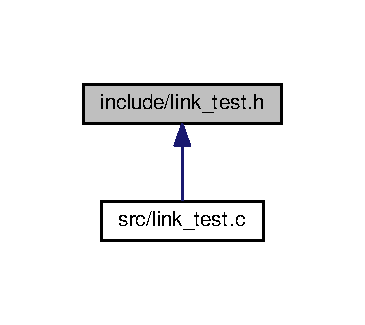
\includegraphics[width=175pt]{link__test_8h__dep__incl}
\end{center}
\end{figure}
\subsection*{Functions}
\begin{DoxyCompactItemize}
\item 
void \hyperlink{link__test_8h_a82c5ee441ad22caad8272212a9e9cc26}{test1\+\_\+link\+\_\+create} ()
\item 
void \hyperlink{link__test_8h_a24b5463da176c3e578b0a0fa8bb1f9f0}{test2\+\_\+link\+\_\+create} ()
\item 
void \hyperlink{link__test_8h_ae0e478a0540bed26befc071591e3ff6c}{test1\+\_\+link\+\_\+set\+\_\+name} ()
\item 
void \hyperlink{link__test_8h_aa66c1e991620a5a758ba6e4d6b4a8b73}{test2\+\_\+link\+\_\+set\+\_\+name} ()
\item 
void \hyperlink{link__test_8h_a8396e33f601deb52c940cb89cd7c6bfe}{test3\+\_\+link\+\_\+set\+\_\+name} ()
\item 
void \hyperlink{link__test_8h_a994aea17881a284366d11ac85d8c60a9}{test1\+\_\+link\+\_\+set\+\_\+link1} ()
\item 
void \hyperlink{link__test_8h_af0f992e367c55a169d9d3f1f4cf58d37}{test2\+\_\+link\+\_\+set\+\_\+link1} ()
\item 
void \hyperlink{link__test_8h_a4e44e515a644abf600efd18aaca7963a}{test1\+\_\+link\+\_\+set\+\_\+link2} ()
\item 
void \hyperlink{link__test_8h_ac4fcf188fc807162c5c279962367faa0}{test2\+\_\+link\+\_\+set\+\_\+link2} ()
\item 
void \hyperlink{link__test_8h_a3b39fdba0c3c967716572bfb01beec27}{test1\+\_\+link\+\_\+set\+\_\+status} ()
\item 
void \hyperlink{link__test_8h_a315ea19cd24434d2153b5df9f372a561}{test2\+\_\+link\+\_\+set\+\_\+status} ()
\item 
void \hyperlink{link__test_8h_a044128db00a5cc385d7157dea8bdf3c3}{test1\+\_\+link\+\_\+get\+\_\+name} ()
\item 
void \hyperlink{link__test_8h_a4efc6cfcdc210e2803f9d285734c571e}{test2\+\_\+link\+\_\+get\+\_\+name} ()
\item 
void \hyperlink{link__test_8h_a4e076db559af261fc8e6994cf9cde12c}{test1\+\_\+link\+\_\+get\+\_\+link1} ()
\item 
void \hyperlink{link__test_8h_a7e180eb974324d38e9bec8bada8d2f7a}{test2\+\_\+link\+\_\+get\+\_\+link1} ()
\item 
void \hyperlink{link__test_8h_a7a8a4b1f4730d248d2c7d648ee4da602}{test1\+\_\+link\+\_\+get\+\_\+link2} ()
\item 
void \hyperlink{link__test_8h_ab74179d7a6e4ceff70117cd20b82c95b}{test2\+\_\+link\+\_\+get\+\_\+link2} ()
\item 
void \hyperlink{link__test_8h_a19c70f79fd51d123173f7aaf6ae50bf8}{test1\+\_\+link\+\_\+get\+\_\+id} ()
\item 
void \hyperlink{link__test_8h_a0f967a1782dd7264e73ad428d22d125d}{test2\+\_\+link\+\_\+get\+\_\+id} ()
\item 
void \hyperlink{link__test_8h_ad4ca02e93472a080362a005ea4840218}{test1\+\_\+link\+\_\+destroy} ()
\item 
void \hyperlink{link__test_8h_afae7294e1213cade145448511cfae536}{test2\+\_\+link\+\_\+destroy} ()
\item 
void \hyperlink{link__test_8h_af99aa73f22b107610780db4877e34448}{test1\+\_\+link\+\_\+print} ()
\item 
void \hyperlink{link__test_8h_a0e42040390aae2aae9f0adee136fe359}{test1\+\_\+link\+\_\+set\+\_\+key} ()
\item 
void \hyperlink{link__test_8h_a502c73e4043204f9fa22f744506bf4e9}{test2\+\_\+link\+\_\+set\+\_\+key} ()
\item 
void \hyperlink{link__test_8h_ab9c08837de834dc139566cefae8e25c2}{test3\+\_\+link\+\_\+set\+\_\+key} ()
\item 
void \hyperlink{link__test_8h_a7dbdc2cfa491e66bba605d96304cf9a9}{test1\+\_\+link\+\_\+get\+\_\+key} ()
\item 
void \hyperlink{link__test_8h_abae02eb503ca35d9198dd4cb2f1c8d5e}{test2\+\_\+link\+\_\+get\+\_\+key} ()
\item 
void \hyperlink{link__test_8h_ac096b0cd1e6b6b44682dc43191a94296}{test3\+\_\+link\+\_\+get\+\_\+key} ()
\end{DoxyCompactItemize}


\subsection{Detailed Description}
It declares the tests for the link module. 

\begin{DoxyAuthor}{Author}
Andres Mena Godino 
\end{DoxyAuthor}
\begin{DoxyVersion}{Version}
2.\+0 
\end{DoxyVersion}
\begin{DoxyDate}{Date}
01-\/03-\/2018 
\end{DoxyDate}
\begin{DoxyCopyright}{Copyright}
G\+NU Public License 
\end{DoxyCopyright}


\subsection{Function Documentation}
\index{link\+\_\+test.\+h@{link\+\_\+test.\+h}!test1\+\_\+link\+\_\+create@{test1\+\_\+link\+\_\+create}}
\index{test1\+\_\+link\+\_\+create@{test1\+\_\+link\+\_\+create}!link\+\_\+test.\+h@{link\+\_\+test.\+h}}
\subsubsection[{\texorpdfstring{test1\+\_\+link\+\_\+create()}{test1_link_create()}}]{\setlength{\rightskip}{0pt plus 5cm}void test1\+\_\+link\+\_\+create (
\begin{DoxyParamCaption}
{}
\end{DoxyParamCaption}
)}\hypertarget{link__test_8h_a82c5ee441ad22caad8272212a9e9cc26}{}\label{link__test_8h_a82c5ee441ad22caad8272212a9e9cc26}
\begin{DoxyRefDesc}{Test}
\item[\hyperlink{test__test000022}{Test}]Test link creation \end{DoxyRefDesc}
\begin{DoxyPrecond}{Precondition}
N\+O\+\_\+\+ID 
\end{DoxyPrecond}
\begin{DoxyPostcond}{Postcondition}
N\+U\+LL pointer to link 
\end{DoxyPostcond}
\index{link\+\_\+test.\+h@{link\+\_\+test.\+h}!test1\+\_\+link\+\_\+destroy@{test1\+\_\+link\+\_\+destroy}}
\index{test1\+\_\+link\+\_\+destroy@{test1\+\_\+link\+\_\+destroy}!link\+\_\+test.\+h@{link\+\_\+test.\+h}}
\subsubsection[{\texorpdfstring{test1\+\_\+link\+\_\+destroy()}{test1_link_destroy()}}]{\setlength{\rightskip}{0pt plus 5cm}void test1\+\_\+link\+\_\+destroy (
\begin{DoxyParamCaption}
{}
\end{DoxyParamCaption}
)}\hypertarget{link__test_8h_ad4ca02e93472a080362a005ea4840218}{}\label{link__test_8h_ad4ca02e93472a080362a005ea4840218}
\begin{DoxyRefDesc}{Test}
\item[\hyperlink{test__test000041}{Test}]Test function for destroying link \end{DoxyRefDesc}
\begin{DoxyPrecond}{Precondition}
N\+U\+LL pointer to link 
\end{DoxyPrecond}
\begin{DoxyPostcond}{Postcondition}
E\+R\+R\+OR 
\end{DoxyPostcond}
\index{link\+\_\+test.\+h@{link\+\_\+test.\+h}!test1\+\_\+link\+\_\+get\+\_\+id@{test1\+\_\+link\+\_\+get\+\_\+id}}
\index{test1\+\_\+link\+\_\+get\+\_\+id@{test1\+\_\+link\+\_\+get\+\_\+id}!link\+\_\+test.\+h@{link\+\_\+test.\+h}}
\subsubsection[{\texorpdfstring{test1\+\_\+link\+\_\+get\+\_\+id()}{test1_link_get_id()}}]{\setlength{\rightskip}{0pt plus 5cm}void test1\+\_\+link\+\_\+get\+\_\+id (
\begin{DoxyParamCaption}
{}
\end{DoxyParamCaption}
)}\hypertarget{link__test_8h_a19c70f79fd51d123173f7aaf6ae50bf8}{}\label{link__test_8h_a19c70f79fd51d123173f7aaf6ae50bf8}
\begin{DoxyRefDesc}{Test}
\item[\hyperlink{test__test000039}{Test}]Test function for getting link id \end{DoxyRefDesc}
\begin{DoxyPrecond}{Precondition}
Pointer to link 
\end{DoxyPrecond}
\begin{DoxyPostcond}{Postcondition}
link\+\_\+\+ID == Supplied link Id 
\end{DoxyPostcond}
\index{link\+\_\+test.\+h@{link\+\_\+test.\+h}!test1\+\_\+link\+\_\+get\+\_\+key@{test1\+\_\+link\+\_\+get\+\_\+key}}
\index{test1\+\_\+link\+\_\+get\+\_\+key@{test1\+\_\+link\+\_\+get\+\_\+key}!link\+\_\+test.\+h@{link\+\_\+test.\+h}}
\subsubsection[{\texorpdfstring{test1\+\_\+link\+\_\+get\+\_\+key()}{test1_link_get_key()}}]{\setlength{\rightskip}{0pt plus 5cm}void test1\+\_\+link\+\_\+get\+\_\+key (
\begin{DoxyParamCaption}
{}
\end{DoxyParamCaption}
)}\hypertarget{link__test_8h_a7dbdc2cfa491e66bba605d96304cf9a9}{}\label{link__test_8h_a7dbdc2cfa491e66bba605d96304cf9a9}
\begin{DoxyRefDesc}{Test}
\item[\hyperlink{test__test000047}{Test}]Test function for getting link key \end{DoxyRefDesc}
\begin{DoxyPrecond}{Precondition}
null Pointer to link 
\end{DoxyPrecond}
\begin{DoxyPostcond}{Postcondition}
N\+O\+\_\+\+ID 
\end{DoxyPostcond}
\index{link\+\_\+test.\+h@{link\+\_\+test.\+h}!test1\+\_\+link\+\_\+get\+\_\+link1@{test1\+\_\+link\+\_\+get\+\_\+link1}}
\index{test1\+\_\+link\+\_\+get\+\_\+link1@{test1\+\_\+link\+\_\+get\+\_\+link1}!link\+\_\+test.\+h@{link\+\_\+test.\+h}}
\subsubsection[{\texorpdfstring{test1\+\_\+link\+\_\+get\+\_\+link1()}{test1_link_get_link1()}}]{\setlength{\rightskip}{0pt plus 5cm}void test1\+\_\+link\+\_\+get\+\_\+link1 (
\begin{DoxyParamCaption}
{}
\end{DoxyParamCaption}
)}\hypertarget{link__test_8h_a4e076db559af261fc8e6994cf9cde12c}{}\label{link__test_8h_a4e076db559af261fc8e6994cf9cde12c}
\begin{DoxyRefDesc}{Test}
\item[\hyperlink{test__test000035}{Test}]Test function for getting first link \end{DoxyRefDesc}
\begin{DoxyPrecond}{Precondition}
Link pointer (with first link created) 
\end{DoxyPrecond}
\begin{DoxyPostcond}{Postcondition}
id of first link 
\end{DoxyPostcond}
\index{link\+\_\+test.\+h@{link\+\_\+test.\+h}!test1\+\_\+link\+\_\+get\+\_\+link2@{test1\+\_\+link\+\_\+get\+\_\+link2}}
\index{test1\+\_\+link\+\_\+get\+\_\+link2@{test1\+\_\+link\+\_\+get\+\_\+link2}!link\+\_\+test.\+h@{link\+\_\+test.\+h}}
\subsubsection[{\texorpdfstring{test1\+\_\+link\+\_\+get\+\_\+link2()}{test1_link_get_link2()}}]{\setlength{\rightskip}{0pt plus 5cm}void test1\+\_\+link\+\_\+get\+\_\+link2 (
\begin{DoxyParamCaption}
{}
\end{DoxyParamCaption}
)}\hypertarget{link__test_8h_a7a8a4b1f4730d248d2c7d648ee4da602}{}\label{link__test_8h_a7a8a4b1f4730d248d2c7d648ee4da602}
\begin{DoxyRefDesc}{Test}
\item[\hyperlink{test__test000037}{Test}]Test function for getting second link \end{DoxyRefDesc}
\begin{DoxyPrecond}{Precondition}
Link pointer (with second link created) 
\end{DoxyPrecond}
\begin{DoxyPostcond}{Postcondition}
id of second link 
\end{DoxyPostcond}
\index{link\+\_\+test.\+h@{link\+\_\+test.\+h}!test1\+\_\+link\+\_\+get\+\_\+name@{test1\+\_\+link\+\_\+get\+\_\+name}}
\index{test1\+\_\+link\+\_\+get\+\_\+name@{test1\+\_\+link\+\_\+get\+\_\+name}!link\+\_\+test.\+h@{link\+\_\+test.\+h}}
\subsubsection[{\texorpdfstring{test1\+\_\+link\+\_\+get\+\_\+name()}{test1_link_get_name()}}]{\setlength{\rightskip}{0pt plus 5cm}void test1\+\_\+link\+\_\+get\+\_\+name (
\begin{DoxyParamCaption}
{}
\end{DoxyParamCaption}
)}\hypertarget{link__test_8h_a044128db00a5cc385d7157dea8bdf3c3}{}\label{link__test_8h_a044128db00a5cc385d7157dea8bdf3c3}
\begin{DoxyRefDesc}{Test}
\item[\hyperlink{test__test000033}{Test}]Test function for link\+\_\+name obtaining \end{DoxyRefDesc}
\begin{DoxyPrecond}{Precondition}
Link pointer 
\end{DoxyPrecond}
\begin{DoxyPostcond}{Postcondition}
String with name 
\end{DoxyPostcond}
\index{link\+\_\+test.\+h@{link\+\_\+test.\+h}!test1\+\_\+link\+\_\+print@{test1\+\_\+link\+\_\+print}}
\index{test1\+\_\+link\+\_\+print@{test1\+\_\+link\+\_\+print}!link\+\_\+test.\+h@{link\+\_\+test.\+h}}
\subsubsection[{\texorpdfstring{test1\+\_\+link\+\_\+print()}{test1_link_print()}}]{\setlength{\rightskip}{0pt plus 5cm}void test1\+\_\+link\+\_\+print (
\begin{DoxyParamCaption}
{}
\end{DoxyParamCaption}
)}\hypertarget{link__test_8h_af99aa73f22b107610780db4877e34448}{}\label{link__test_8h_af99aa73f22b107610780db4877e34448}
\begin{DoxyRefDesc}{Test}
\item[\hyperlink{test__test000043}{Test}]Test function for printing link \end{DoxyRefDesc}
\begin{DoxyPrecond}{Precondition}
N\+U\+LL pointer to link 
\end{DoxyPrecond}
\begin{DoxyPostcond}{Postcondition}
E\+R\+R\+OR 
\end{DoxyPostcond}
\index{link\+\_\+test.\+h@{link\+\_\+test.\+h}!test1\+\_\+link\+\_\+set\+\_\+key@{test1\+\_\+link\+\_\+set\+\_\+key}}
\index{test1\+\_\+link\+\_\+set\+\_\+key@{test1\+\_\+link\+\_\+set\+\_\+key}!link\+\_\+test.\+h@{link\+\_\+test.\+h}}
\subsubsection[{\texorpdfstring{test1\+\_\+link\+\_\+set\+\_\+key()}{test1_link_set_key()}}]{\setlength{\rightskip}{0pt plus 5cm}void test1\+\_\+link\+\_\+set\+\_\+key (
\begin{DoxyParamCaption}
{}
\end{DoxyParamCaption}
)}\hypertarget{link__test_8h_a0e42040390aae2aae9f0adee136fe359}{}\label{link__test_8h_a0e42040390aae2aae9f0adee136fe359}
\begin{DoxyRefDesc}{Test}
\item[\hyperlink{test__test000044}{Test}]Test function for setting link key \end{DoxyRefDesc}
\begin{DoxyPrecond}{Precondition}
N\+U\+LL pointer to link 
\end{DoxyPrecond}
\begin{DoxyPostcond}{Postcondition}
E\+R\+R\+OR 
\end{DoxyPostcond}
\index{link\+\_\+test.\+h@{link\+\_\+test.\+h}!test1\+\_\+link\+\_\+set\+\_\+link1@{test1\+\_\+link\+\_\+set\+\_\+link1}}
\index{test1\+\_\+link\+\_\+set\+\_\+link1@{test1\+\_\+link\+\_\+set\+\_\+link1}!link\+\_\+test.\+h@{link\+\_\+test.\+h}}
\subsubsection[{\texorpdfstring{test1\+\_\+link\+\_\+set\+\_\+link1()}{test1_link_set_link1()}}]{\setlength{\rightskip}{0pt plus 5cm}void test1\+\_\+link\+\_\+set\+\_\+link1 (
\begin{DoxyParamCaption}
{}
\end{DoxyParamCaption}
)}\hypertarget{link__test_8h_a994aea17881a284366d11ac85d8c60a9}{}\label{link__test_8h_a994aea17881a284366d11ac85d8c60a9}
\begin{DoxyRefDesc}{Test}
\item[\hyperlink{test__test000027}{Test}]Test function for setting first link \end{DoxyRefDesc}
\begin{DoxyPrecond}{Precondition}
pointer to link and id 
\end{DoxyPrecond}
\begin{DoxyPostcond}{Postcondition}
Ouput==OK 
\end{DoxyPostcond}
\index{link\+\_\+test.\+h@{link\+\_\+test.\+h}!test1\+\_\+link\+\_\+set\+\_\+link2@{test1\+\_\+link\+\_\+set\+\_\+link2}}
\index{test1\+\_\+link\+\_\+set\+\_\+link2@{test1\+\_\+link\+\_\+set\+\_\+link2}!link\+\_\+test.\+h@{link\+\_\+test.\+h}}
\subsubsection[{\texorpdfstring{test1\+\_\+link\+\_\+set\+\_\+link2()}{test1_link_set_link2()}}]{\setlength{\rightskip}{0pt plus 5cm}void test1\+\_\+link\+\_\+set\+\_\+link2 (
\begin{DoxyParamCaption}
{}
\end{DoxyParamCaption}
)}\hypertarget{link__test_8h_a4e44e515a644abf600efd18aaca7963a}{}\label{link__test_8h_a4e44e515a644abf600efd18aaca7963a}
\begin{DoxyRefDesc}{Test}
\item[\hyperlink{test__test000029}{Test}]Test function for setting second link \end{DoxyRefDesc}
\begin{DoxyPrecond}{Precondition}
pointer to link and id 
\end{DoxyPrecond}
\begin{DoxyPostcond}{Postcondition}
Ouput==OK 
\end{DoxyPostcond}
\index{link\+\_\+test.\+h@{link\+\_\+test.\+h}!test1\+\_\+link\+\_\+set\+\_\+name@{test1\+\_\+link\+\_\+set\+\_\+name}}
\index{test1\+\_\+link\+\_\+set\+\_\+name@{test1\+\_\+link\+\_\+set\+\_\+name}!link\+\_\+test.\+h@{link\+\_\+test.\+h}}
\subsubsection[{\texorpdfstring{test1\+\_\+link\+\_\+set\+\_\+name()}{test1_link_set_name()}}]{\setlength{\rightskip}{0pt plus 5cm}void test1\+\_\+link\+\_\+set\+\_\+name (
\begin{DoxyParamCaption}
{}
\end{DoxyParamCaption}
)}\hypertarget{link__test_8h_ae0e478a0540bed26befc071591e3ff6c}{}\label{link__test_8h_ae0e478a0540bed26befc071591e3ff6c}
\begin{DoxyRefDesc}{Test}
\item[\hyperlink{test__test000024}{Test}]Test function for link\+\_\+name setting \end{DoxyRefDesc}
\begin{DoxyPrecond}{Precondition}
pointer to link and string with link name 
\end{DoxyPrecond}
\begin{DoxyPostcond}{Postcondition}
Ouput==OK 
\end{DoxyPostcond}
\index{link\+\_\+test.\+h@{link\+\_\+test.\+h}!test1\+\_\+link\+\_\+set\+\_\+status@{test1\+\_\+link\+\_\+set\+\_\+status}}
\index{test1\+\_\+link\+\_\+set\+\_\+status@{test1\+\_\+link\+\_\+set\+\_\+status}!link\+\_\+test.\+h@{link\+\_\+test.\+h}}
\subsubsection[{\texorpdfstring{test1\+\_\+link\+\_\+set\+\_\+status()}{test1_link_set_status()}}]{\setlength{\rightskip}{0pt plus 5cm}void test1\+\_\+link\+\_\+set\+\_\+status (
\begin{DoxyParamCaption}
{}
\end{DoxyParamCaption}
)}\hypertarget{link__test_8h_a3b39fdba0c3c967716572bfb01beec27}{}\label{link__test_8h_a3b39fdba0c3c967716572bfb01beec27}
\begin{DoxyRefDesc}{Test}
\item[\hyperlink{test__test000031}{Test}]Test function for setting status of link \end{DoxyRefDesc}
\begin{DoxyPrecond}{Precondition}
Pointer to link and L\+I\+N\+K\+\_\+\+ST 
\end{DoxyPrecond}
\begin{DoxyPostcond}{Postcondition}
Ouput==OK 
\end{DoxyPostcond}
\index{link\+\_\+test.\+h@{link\+\_\+test.\+h}!test2\+\_\+link\+\_\+create@{test2\+\_\+link\+\_\+create}}
\index{test2\+\_\+link\+\_\+create@{test2\+\_\+link\+\_\+create}!link\+\_\+test.\+h@{link\+\_\+test.\+h}}
\subsubsection[{\texorpdfstring{test2\+\_\+link\+\_\+create()}{test2_link_create()}}]{\setlength{\rightskip}{0pt plus 5cm}void test2\+\_\+link\+\_\+create (
\begin{DoxyParamCaption}
{}
\end{DoxyParamCaption}
)}\hypertarget{link__test_8h_a24b5463da176c3e578b0a0fa8bb1f9f0}{}\label{link__test_8h_a24b5463da176c3e578b0a0fa8bb1f9f0}
\begin{DoxyRefDesc}{Test}
\item[\hyperlink{test__test000023}{Test}]Test link creation \end{DoxyRefDesc}
\begin{DoxyPrecond}{Precondition}
ID 
\end{DoxyPrecond}
\begin{DoxyPostcond}{Postcondition}
link ID == id introduced 
\end{DoxyPostcond}
\index{link\+\_\+test.\+h@{link\+\_\+test.\+h}!test2\+\_\+link\+\_\+destroy@{test2\+\_\+link\+\_\+destroy}}
\index{test2\+\_\+link\+\_\+destroy@{test2\+\_\+link\+\_\+destroy}!link\+\_\+test.\+h@{link\+\_\+test.\+h}}
\subsubsection[{\texorpdfstring{test2\+\_\+link\+\_\+destroy()}{test2_link_destroy()}}]{\setlength{\rightskip}{0pt plus 5cm}void test2\+\_\+link\+\_\+destroy (
\begin{DoxyParamCaption}
{}
\end{DoxyParamCaption}
)}\hypertarget{link__test_8h_afae7294e1213cade145448511cfae536}{}\label{link__test_8h_afae7294e1213cade145448511cfae536}
\begin{DoxyRefDesc}{Test}
\item[\hyperlink{test__test000042}{Test}]Test function for destroying link \end{DoxyRefDesc}
\begin{DoxyPrecond}{Precondition}
pointer to link 
\end{DoxyPrecond}
\begin{DoxyPostcond}{Postcondition}
OK 
\end{DoxyPostcond}
\index{link\+\_\+test.\+h@{link\+\_\+test.\+h}!test2\+\_\+link\+\_\+get\+\_\+id@{test2\+\_\+link\+\_\+get\+\_\+id}}
\index{test2\+\_\+link\+\_\+get\+\_\+id@{test2\+\_\+link\+\_\+get\+\_\+id}!link\+\_\+test.\+h@{link\+\_\+test.\+h}}
\subsubsection[{\texorpdfstring{test2\+\_\+link\+\_\+get\+\_\+id()}{test2_link_get_id()}}]{\setlength{\rightskip}{0pt plus 5cm}void test2\+\_\+link\+\_\+get\+\_\+id (
\begin{DoxyParamCaption}
{}
\end{DoxyParamCaption}
)}\hypertarget{link__test_8h_a0f967a1782dd7264e73ad428d22d125d}{}\label{link__test_8h_a0f967a1782dd7264e73ad428d22d125d}
\begin{DoxyRefDesc}{Test}
\item[\hyperlink{test__test000040}{Test}]Test function for getting link id \end{DoxyRefDesc}
\begin{DoxyPrecond}{Precondition}
N\+U\+LL pointer to link 
\end{DoxyPrecond}
\begin{DoxyPostcond}{Postcondition}
N\+O\+\_\+\+ID 
\end{DoxyPostcond}
\index{link\+\_\+test.\+h@{link\+\_\+test.\+h}!test2\+\_\+link\+\_\+get\+\_\+key@{test2\+\_\+link\+\_\+get\+\_\+key}}
\index{test2\+\_\+link\+\_\+get\+\_\+key@{test2\+\_\+link\+\_\+get\+\_\+key}!link\+\_\+test.\+h@{link\+\_\+test.\+h}}
\subsubsection[{\texorpdfstring{test2\+\_\+link\+\_\+get\+\_\+key()}{test2_link_get_key()}}]{\setlength{\rightskip}{0pt plus 5cm}void test2\+\_\+link\+\_\+get\+\_\+key (
\begin{DoxyParamCaption}
{}
\end{DoxyParamCaption}
)}\hypertarget{link__test_8h_abae02eb503ca35d9198dd4cb2f1c8d5e}{}\label{link__test_8h_abae02eb503ca35d9198dd4cb2f1c8d5e}
\begin{DoxyRefDesc}{Test}
\item[\hyperlink{test__test000048}{Test}]Test function for getting link key \end{DoxyRefDesc}
\begin{DoxyPrecond}{Precondition}
Pointer to link 
\end{DoxyPrecond}
\begin{DoxyPostcond}{Postcondition}
Zero 
\end{DoxyPostcond}
\index{link\+\_\+test.\+h@{link\+\_\+test.\+h}!test2\+\_\+link\+\_\+get\+\_\+link1@{test2\+\_\+link\+\_\+get\+\_\+link1}}
\index{test2\+\_\+link\+\_\+get\+\_\+link1@{test2\+\_\+link\+\_\+get\+\_\+link1}!link\+\_\+test.\+h@{link\+\_\+test.\+h}}
\subsubsection[{\texorpdfstring{test2\+\_\+link\+\_\+get\+\_\+link1()}{test2_link_get_link1()}}]{\setlength{\rightskip}{0pt plus 5cm}void test2\+\_\+link\+\_\+get\+\_\+link1 (
\begin{DoxyParamCaption}
{}
\end{DoxyParamCaption}
)}\hypertarget{link__test_8h_a7e180eb974324d38e9bec8bada8d2f7a}{}\label{link__test_8h_a7e180eb974324d38e9bec8bada8d2f7a}
\begin{DoxyRefDesc}{Test}
\item[\hyperlink{test__test000036}{Test}]Test function for getting first link \end{DoxyRefDesc}
\begin{DoxyPrecond}{Precondition}
N\+U\+LL link pointer 
\end{DoxyPrecond}
\begin{DoxyPostcond}{Postcondition}
N\+O\+\_\+\+ID 
\end{DoxyPostcond}
\index{link\+\_\+test.\+h@{link\+\_\+test.\+h}!test2\+\_\+link\+\_\+get\+\_\+link2@{test2\+\_\+link\+\_\+get\+\_\+link2}}
\index{test2\+\_\+link\+\_\+get\+\_\+link2@{test2\+\_\+link\+\_\+get\+\_\+link2}!link\+\_\+test.\+h@{link\+\_\+test.\+h}}
\subsubsection[{\texorpdfstring{test2\+\_\+link\+\_\+get\+\_\+link2()}{test2_link_get_link2()}}]{\setlength{\rightskip}{0pt plus 5cm}void test2\+\_\+link\+\_\+get\+\_\+link2 (
\begin{DoxyParamCaption}
{}
\end{DoxyParamCaption}
)}\hypertarget{link__test_8h_ab74179d7a6e4ceff70117cd20b82c95b}{}\label{link__test_8h_ab74179d7a6e4ceff70117cd20b82c95b}
\begin{DoxyRefDesc}{Test}
\item[\hyperlink{test__test000038}{Test}]Test function for getting second link \end{DoxyRefDesc}
\begin{DoxyPrecond}{Precondition}
N\+U\+LL link pointer 
\end{DoxyPrecond}
\begin{DoxyPostcond}{Postcondition}
N\+O\+\_\+\+ID 
\end{DoxyPostcond}
\index{link\+\_\+test.\+h@{link\+\_\+test.\+h}!test2\+\_\+link\+\_\+get\+\_\+name@{test2\+\_\+link\+\_\+get\+\_\+name}}
\index{test2\+\_\+link\+\_\+get\+\_\+name@{test2\+\_\+link\+\_\+get\+\_\+name}!link\+\_\+test.\+h@{link\+\_\+test.\+h}}
\subsubsection[{\texorpdfstring{test2\+\_\+link\+\_\+get\+\_\+name()}{test2_link_get_name()}}]{\setlength{\rightskip}{0pt plus 5cm}void test2\+\_\+link\+\_\+get\+\_\+name (
\begin{DoxyParamCaption}
{}
\end{DoxyParamCaption}
)}\hypertarget{link__test_8h_a4efc6cfcdc210e2803f9d285734c571e}{}\label{link__test_8h_a4efc6cfcdc210e2803f9d285734c571e}
\begin{DoxyRefDesc}{Test}
\item[\hyperlink{test__test000034}{Test}]Test function for link\+\_\+name obtaining \end{DoxyRefDesc}
\begin{DoxyPrecond}{Precondition}
N\+U\+LL link pointer 
\end{DoxyPrecond}
\begin{DoxyPostcond}{Postcondition}
N\+U\+LL string 
\end{DoxyPostcond}
\index{link\+\_\+test.\+h@{link\+\_\+test.\+h}!test2\+\_\+link\+\_\+set\+\_\+key@{test2\+\_\+link\+\_\+set\+\_\+key}}
\index{test2\+\_\+link\+\_\+set\+\_\+key@{test2\+\_\+link\+\_\+set\+\_\+key}!link\+\_\+test.\+h@{link\+\_\+test.\+h}}
\subsubsection[{\texorpdfstring{test2\+\_\+link\+\_\+set\+\_\+key()}{test2_link_set_key()}}]{\setlength{\rightskip}{0pt plus 5cm}void test2\+\_\+link\+\_\+set\+\_\+key (
\begin{DoxyParamCaption}
{}
\end{DoxyParamCaption}
)}\hypertarget{link__test_8h_a502c73e4043204f9fa22f744506bf4e9}{}\label{link__test_8h_a502c73e4043204f9fa22f744506bf4e9}
\begin{DoxyRefDesc}{Test}
\item[\hyperlink{test__test000045}{Test}]Test function for setting link key \end{DoxyRefDesc}
\begin{DoxyPrecond}{Precondition}
Pointer to link and N\+O\+\_\+\+ID 
\end{DoxyPrecond}
\begin{DoxyPostcond}{Postcondition}
E\+R\+R\+OR 
\end{DoxyPostcond}
\index{link\+\_\+test.\+h@{link\+\_\+test.\+h}!test2\+\_\+link\+\_\+set\+\_\+link1@{test2\+\_\+link\+\_\+set\+\_\+link1}}
\index{test2\+\_\+link\+\_\+set\+\_\+link1@{test2\+\_\+link\+\_\+set\+\_\+link1}!link\+\_\+test.\+h@{link\+\_\+test.\+h}}
\subsubsection[{\texorpdfstring{test2\+\_\+link\+\_\+set\+\_\+link1()}{test2_link_set_link1()}}]{\setlength{\rightskip}{0pt plus 5cm}void test2\+\_\+link\+\_\+set\+\_\+link1 (
\begin{DoxyParamCaption}
{}
\end{DoxyParamCaption}
)}\hypertarget{link__test_8h_af0f992e367c55a169d9d3f1f4cf58d37}{}\label{link__test_8h_af0f992e367c55a169d9d3f1f4cf58d37}
\begin{DoxyRefDesc}{Test}
\item[\hyperlink{test__test000028}{Test}]Test function for setting first link \end{DoxyRefDesc}
\begin{DoxyPrecond}{Precondition}
N\+U\+LL pointer to link and id 
\end{DoxyPrecond}
\begin{DoxyPostcond}{Postcondition}
Ouput==E\+R\+R\+OR 
\end{DoxyPostcond}
\index{link\+\_\+test.\+h@{link\+\_\+test.\+h}!test2\+\_\+link\+\_\+set\+\_\+link2@{test2\+\_\+link\+\_\+set\+\_\+link2}}
\index{test2\+\_\+link\+\_\+set\+\_\+link2@{test2\+\_\+link\+\_\+set\+\_\+link2}!link\+\_\+test.\+h@{link\+\_\+test.\+h}}
\subsubsection[{\texorpdfstring{test2\+\_\+link\+\_\+set\+\_\+link2()}{test2_link_set_link2()}}]{\setlength{\rightskip}{0pt plus 5cm}void test2\+\_\+link\+\_\+set\+\_\+link2 (
\begin{DoxyParamCaption}
{}
\end{DoxyParamCaption}
)}\hypertarget{link__test_8h_ac4fcf188fc807162c5c279962367faa0}{}\label{link__test_8h_ac4fcf188fc807162c5c279962367faa0}
\begin{DoxyRefDesc}{Test}
\item[\hyperlink{test__test000030}{Test}]Test function for setting second link \end{DoxyRefDesc}
\begin{DoxyPrecond}{Precondition}
N\+U\+LL pointer to link and id 
\end{DoxyPrecond}
\begin{DoxyPostcond}{Postcondition}
Ouput==E\+R\+R\+OR 
\end{DoxyPostcond}
\index{link\+\_\+test.\+h@{link\+\_\+test.\+h}!test2\+\_\+link\+\_\+set\+\_\+name@{test2\+\_\+link\+\_\+set\+\_\+name}}
\index{test2\+\_\+link\+\_\+set\+\_\+name@{test2\+\_\+link\+\_\+set\+\_\+name}!link\+\_\+test.\+h@{link\+\_\+test.\+h}}
\subsubsection[{\texorpdfstring{test2\+\_\+link\+\_\+set\+\_\+name()}{test2_link_set_name()}}]{\setlength{\rightskip}{0pt plus 5cm}void test2\+\_\+link\+\_\+set\+\_\+name (
\begin{DoxyParamCaption}
{}
\end{DoxyParamCaption}
)}\hypertarget{link__test_8h_aa66c1e991620a5a758ba6e4d6b4a8b73}{}\label{link__test_8h_aa66c1e991620a5a758ba6e4d6b4a8b73}
\begin{DoxyRefDesc}{Test}
\item[\hyperlink{test__test000025}{Test}]Test function for link\+\_\+name setting \end{DoxyRefDesc}
\begin{DoxyPrecond}{Precondition}
N\+U\+LL pointer to link and string with link name 
\end{DoxyPrecond}
\begin{DoxyPostcond}{Postcondition}
Ouput==E\+R\+R\+OR 
\end{DoxyPostcond}
\index{link\+\_\+test.\+h@{link\+\_\+test.\+h}!test2\+\_\+link\+\_\+set\+\_\+status@{test2\+\_\+link\+\_\+set\+\_\+status}}
\index{test2\+\_\+link\+\_\+set\+\_\+status@{test2\+\_\+link\+\_\+set\+\_\+status}!link\+\_\+test.\+h@{link\+\_\+test.\+h}}
\subsubsection[{\texorpdfstring{test2\+\_\+link\+\_\+set\+\_\+status()}{test2_link_set_status()}}]{\setlength{\rightskip}{0pt plus 5cm}void test2\+\_\+link\+\_\+set\+\_\+status (
\begin{DoxyParamCaption}
{}
\end{DoxyParamCaption}
)}\hypertarget{link__test_8h_a315ea19cd24434d2153b5df9f372a561}{}\label{link__test_8h_a315ea19cd24434d2153b5df9f372a561}
\begin{DoxyRefDesc}{Test}
\item[\hyperlink{test__test000032}{Test}]Test function for setting status of link \end{DoxyRefDesc}
\begin{DoxyPrecond}{Precondition}
N\+U\+LL pointer to link and L\+I\+N\+K\+\_\+\+ST 
\end{DoxyPrecond}
\begin{DoxyPostcond}{Postcondition}
Ouput==E\+R\+R\+OR 
\end{DoxyPostcond}
\index{link\+\_\+test.\+h@{link\+\_\+test.\+h}!test3\+\_\+link\+\_\+get\+\_\+key@{test3\+\_\+link\+\_\+get\+\_\+key}}
\index{test3\+\_\+link\+\_\+get\+\_\+key@{test3\+\_\+link\+\_\+get\+\_\+key}!link\+\_\+test.\+h@{link\+\_\+test.\+h}}
\subsubsection[{\texorpdfstring{test3\+\_\+link\+\_\+get\+\_\+key()}{test3_link_get_key()}}]{\setlength{\rightskip}{0pt plus 5cm}void test3\+\_\+link\+\_\+get\+\_\+key (
\begin{DoxyParamCaption}
{}
\end{DoxyParamCaption}
)}\hypertarget{link__test_8h_ac096b0cd1e6b6b44682dc43191a94296}{}\label{link__test_8h_ac096b0cd1e6b6b44682dc43191a94296}
\begin{DoxyRefDesc}{Test}
\item[\hyperlink{test__test000049}{Test}]Test function for getting link key \end{DoxyRefDesc}
\begin{DoxyPrecond}{Precondition}
Pointer to link and introduced id 
\end{DoxyPrecond}
\begin{DoxyPostcond}{Postcondition}
Id previosuly introduced 
\end{DoxyPostcond}
\index{link\+\_\+test.\+h@{link\+\_\+test.\+h}!test3\+\_\+link\+\_\+set\+\_\+key@{test3\+\_\+link\+\_\+set\+\_\+key}}
\index{test3\+\_\+link\+\_\+set\+\_\+key@{test3\+\_\+link\+\_\+set\+\_\+key}!link\+\_\+test.\+h@{link\+\_\+test.\+h}}
\subsubsection[{\texorpdfstring{test3\+\_\+link\+\_\+set\+\_\+key()}{test3_link_set_key()}}]{\setlength{\rightskip}{0pt plus 5cm}void test3\+\_\+link\+\_\+set\+\_\+key (
\begin{DoxyParamCaption}
{}
\end{DoxyParamCaption}
)}\hypertarget{link__test_8h_ab9c08837de834dc139566cefae8e25c2}{}\label{link__test_8h_ab9c08837de834dc139566cefae8e25c2}
\begin{DoxyRefDesc}{Test}
\item[\hyperlink{test__test000046}{Test}]Test function for setting link key \end{DoxyRefDesc}
\begin{DoxyPrecond}{Precondition}
Pointer to link and ID 
\end{DoxyPrecond}
\begin{DoxyPostcond}{Postcondition}
OK 
\end{DoxyPostcond}
\index{link\+\_\+test.\+h@{link\+\_\+test.\+h}!test3\+\_\+link\+\_\+set\+\_\+name@{test3\+\_\+link\+\_\+set\+\_\+name}}
\index{test3\+\_\+link\+\_\+set\+\_\+name@{test3\+\_\+link\+\_\+set\+\_\+name}!link\+\_\+test.\+h@{link\+\_\+test.\+h}}
\subsubsection[{\texorpdfstring{test3\+\_\+link\+\_\+set\+\_\+name()}{test3_link_set_name()}}]{\setlength{\rightskip}{0pt plus 5cm}void test3\+\_\+link\+\_\+set\+\_\+name (
\begin{DoxyParamCaption}
{}
\end{DoxyParamCaption}
)}\hypertarget{link__test_8h_a8396e33f601deb52c940cb89cd7c6bfe}{}\label{link__test_8h_a8396e33f601deb52c940cb89cd7c6bfe}
\begin{DoxyRefDesc}{Test}
\item[\hyperlink{test__test000026}{Test}]Test function for link\+\_\+name setting \end{DoxyRefDesc}
\begin{DoxyPrecond}{Precondition}
pointer to link and N\+U\+LL string of characters 
\end{DoxyPrecond}
\begin{DoxyPostcond}{Postcondition}
Ouput==E\+R\+R\+OR 
\end{DoxyPostcond}

\hypertarget{object_8h}{}\section{include/object.h File Reference}
\label{object_8h}\index{include/object.\+h@{include/object.\+h}}


Implements the game object commands.  


{\ttfamily \#include $<$stdio.\+h$>$}\\*
{\ttfamily \#include \char`\"{}types.\+h\char`\"{}}\\*
Include dependency graph for object.\+h\+:
\nopagebreak
\begin{figure}[H]
\begin{center}
\leavevmode
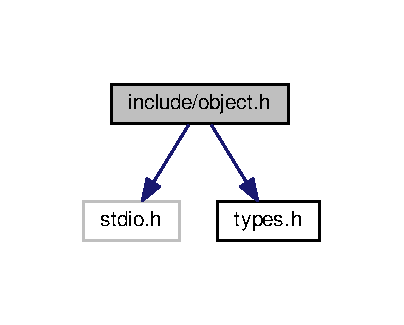
\includegraphics[width=194pt]{object_8h__incl}
\end{center}
\end{figure}
This graph shows which files directly or indirectly include this file\+:
\nopagebreak
\begin{figure}[H]
\begin{center}
\leavevmode
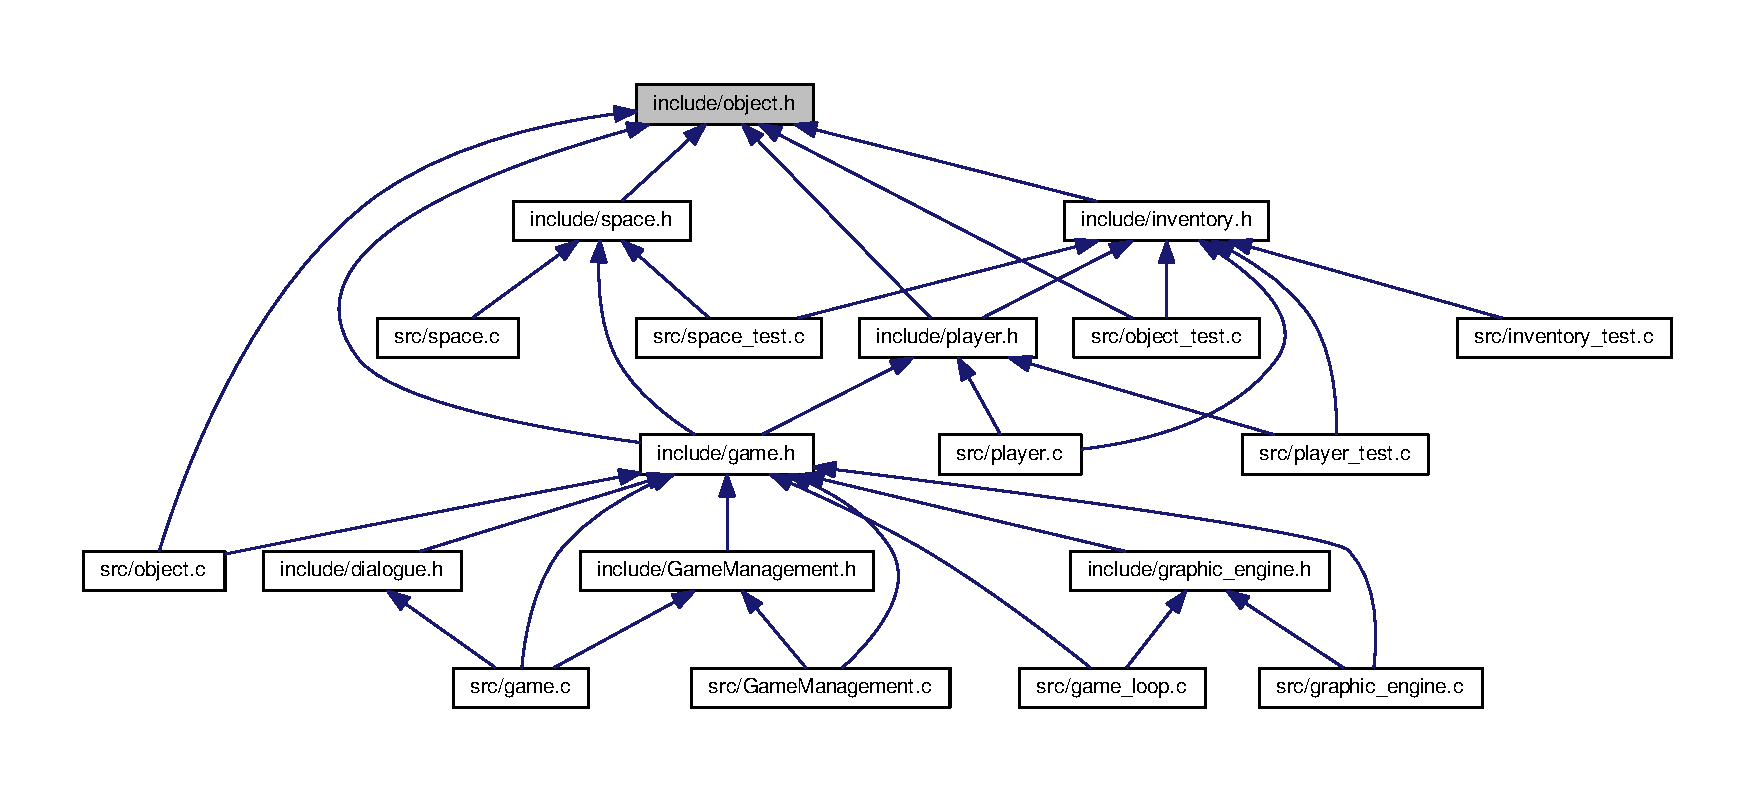
\includegraphics[width=350pt]{object_8h__dep__incl}
\end{center}
\end{figure}
\subsection*{Macros}
\begin{DoxyCompactItemize}
\item 
\#define \hyperlink{object_8h_a88b1ded1b83576bfb0683aeab25ae052}{M\+A\+X\+O\+B\+J\+N\+A\+ME}~30
\end{DoxyCompactItemize}
\subsection*{Typedefs}
\begin{DoxyCompactItemize}
\item 
typedef struct \hyperlink{struct__Object}{\+\_\+\+Object} \hyperlink{object_8h_a7f8bbcda919b65ce67f92fba08e0212f}{Object}
\begin{DoxyCompactList}\small\item\em object of the game \end{DoxyCompactList}\end{DoxyCompactItemize}
\subsection*{Functions}
\begin{DoxyCompactItemize}
\item 
\hyperlink{object_8h_a7f8bbcda919b65ce67f92fba08e0212f}{Object} $\ast$ \hyperlink{object_8h_abb0cd30fca5fbddf137c6c04df66bbc7}{object\+\_\+create} (\hyperlink{types_8h_a845e604fb28f7e3d97549da3448149d3}{Id} id)
\begin{DoxyCompactList}\small\item\em creates an object \end{DoxyCompactList}\item 
void \hyperlink{object_8h_a26c44b44a0fbeb25ef0984614c752dfc}{object\+\_\+destroy} (\hyperlink{object_8h_a7f8bbcda919b65ce67f92fba08e0212f}{Object} $\ast$o)
\begin{DoxyCompactList}\small\item\em frees memory \end{DoxyCompactList}\item 
\hyperlink{types_8h_a845e604fb28f7e3d97549da3448149d3}{Id} \hyperlink{object_8h_a9752f952077d92e3caad01bc0ef88219}{object\+\_\+get\+\_\+id} (\hyperlink{object_8h_a7f8bbcda919b65ce67f92fba08e0212f}{Object} $\ast$o)
\begin{DoxyCompactList}\small\item\em gets the id of an object \end{DoxyCompactList}\item 
char $\ast$ \hyperlink{object_8h_a1d9c831b8ea3bc3667c4bf166bd458dd}{object\+\_\+get\+\_\+name} (\hyperlink{object_8h_a7f8bbcda919b65ce67f92fba08e0212f}{Object} $\ast$o)
\begin{DoxyCompactList}\small\item\em gets the name of an object \end{DoxyCompactList}\item 
\hyperlink{types_8h_a845e604fb28f7e3d97549da3448149d3}{Id} \hyperlink{object_8h_acf961fc31f1928c71c59d96a2ff0d1cd}{object\+\_\+get\+\_\+location} (\hyperlink{object_8h_a7f8bbcda919b65ce67f92fba08e0212f}{Object} $\ast$o)
\begin{DoxyCompactList}\small\item\em gets the location of an object \end{DoxyCompactList}\item 
\hyperlink{types_8h_a32c27cc471df37f4fc818d65de0a56c4}{S\+T\+A\+T\+US} \hyperlink{object_8h_a839f09c377c10dc0138e844c5c2f9324}{object\+\_\+set\+\_\+name} (\hyperlink{object_8h_a7f8bbcda919b65ce67f92fba08e0212f}{Object} $\ast$o, char $\ast$name)
\begin{DoxyCompactList}\small\item\em sets the name of an object \end{DoxyCompactList}\item 
\hyperlink{types_8h_a32c27cc471df37f4fc818d65de0a56c4}{S\+T\+A\+T\+US} \hyperlink{object_8h_a8d07c8e2c06363c4a41b36198e57fc10}{object\+\_\+set\+\_\+id} (\hyperlink{object_8h_a7f8bbcda919b65ce67f92fba08e0212f}{Object} $\ast$o, \hyperlink{types_8h_a845e604fb28f7e3d97549da3448149d3}{Id} id)
\begin{DoxyCompactList}\small\item\em sets an id for an object \end{DoxyCompactList}\item 
\hyperlink{types_8h_a32c27cc471df37f4fc818d65de0a56c4}{S\+T\+A\+T\+US} \hyperlink{object_8h_a0a4d910353d6334df5831468ff5524f9}{object\+\_\+set\+\_\+location} (\hyperlink{object_8h_a7f8bbcda919b65ce67f92fba08e0212f}{Object} $\ast$o, \hyperlink{types_8h_a845e604fb28f7e3d97549da3448149d3}{Id} id)
\begin{DoxyCompactList}\small\item\em sets location \end{DoxyCompactList}\item 
\hyperlink{types_8h_a32c27cc471df37f4fc818d65de0a56c4}{S\+T\+A\+T\+US} \hyperlink{object_8h_a4a4f1a7f753ec9295548c099ec755718}{object\+\_\+print} (\hyperlink{object_8h_a7f8bbcda919b65ce67f92fba08e0212f}{Object} $\ast$o, F\+I\+LE $\ast$f)
\begin{DoxyCompactList}\small\item\em prints an object \end{DoxyCompactList}\item 
char $\ast$ \hyperlink{object_8h_a66311e7f25b9eba333bc2ddec8aba14f}{object\+\_\+get\+\_\+original\+\_\+description} (\hyperlink{object_8h_a7f8bbcda919b65ce67f92fba08e0212f}{Object} $\ast$o)
\begin{DoxyCompactList}\small\item\em gets description \end{DoxyCompactList}\item 
\hyperlink{types_8h_a32c27cc471df37f4fc818d65de0a56c4}{S\+T\+A\+T\+US} \hyperlink{object_8h_ae70e3276ecd61873f1f0a540ee785e3f}{object\+\_\+set\+\_\+original\+\_\+description} (\hyperlink{object_8h_a7f8bbcda919b65ce67f92fba08e0212f}{Object} $\ast$o, char $\ast$description)
\begin{DoxyCompactList}\small\item\em sets description \end{DoxyCompactList}\item 
\hyperlink{types_8h_a32c27cc471df37f4fc818d65de0a56c4}{S\+T\+A\+T\+US} \hyperlink{object_8h_a169ccd54cbbdc828f67fd819ede6000d}{object\+\_\+set\+\_\+original\+\_\+position} (\hyperlink{object_8h_a7f8bbcda919b65ce67f92fba08e0212f}{Object} $\ast$o, \hyperlink{types_8h_a845e604fb28f7e3d97549da3448149d3}{Id} id)
\begin{DoxyCompactList}\small\item\em sets position \end{DoxyCompactList}\item 
\hyperlink{types_8h_a845e604fb28f7e3d97549da3448149d3}{Id} \hyperlink{object_8h_a0f486e12d9d5db67ed56f40b5cdc0f7f}{object\+\_\+get\+\_\+original\+\_\+position} (\hyperlink{object_8h_a7f8bbcda919b65ce67f92fba08e0212f}{Object} $\ast$o)
\begin{DoxyCompactList}\small\item\em gets description \end{DoxyCompactList}\item 
\hyperlink{types_8h_a32c27cc471df37f4fc818d65de0a56c4}{S\+T\+A\+T\+US} \hyperlink{object_8h_a684297abcecea4f985c22c09d7a2683e}{object\+\_\+set\+\_\+moved\+\_\+description} (\hyperlink{object_8h_a7f8bbcda919b65ce67f92fba08e0212f}{Object} $\ast$o, char $\ast$description)
\begin{DoxyCompactList}\small\item\em sets description \end{DoxyCompactList}\item 
\hyperlink{types_8h_a32c27cc471df37f4fc818d65de0a56c4}{S\+T\+A\+T\+US} \hyperlink{object_8h_a259c9fd13df4766071af2e0a0d7a1a87}{object\+\_\+set\+\_\+prop\+\_\+\+Movable} (\hyperlink{object_8h_a7f8bbcda919b65ce67f92fba08e0212f}{Object} $\ast$o, \hyperlink{types_8h_a3e5b8192e7d9ffaf3542f1210aec18dd}{B\+O\+OL} st)
\begin{DoxyCompactList}\small\item\em sets status of mobility \end{DoxyCompactList}\item 
\hyperlink{types_8h_a3e5b8192e7d9ffaf3542f1210aec18dd}{B\+O\+OL} \hyperlink{object_8h_a98f562a9ee1801aea8f5f0212bdba008}{object\+\_\+get\+\_\+prop\+\_\+\+Movable} (\hyperlink{object_8h_a7f8bbcda919b65ce67f92fba08e0212f}{Object} $\ast$o)
\begin{DoxyCompactList}\small\item\em gets the mobility status \end{DoxyCompactList}\item 
\hyperlink{types_8h_a32c27cc471df37f4fc818d65de0a56c4}{S\+T\+A\+T\+US} \hyperlink{object_8h_a2b49f5b9d0eba678c034bdf9c91b36b1}{object\+\_\+set\+\_\+prop\+\_\+\+Moved} (\hyperlink{object_8h_a7f8bbcda919b65ce67f92fba08e0212f}{Object} $\ast$o, \hyperlink{types_8h_a3e5b8192e7d9ffaf3542f1210aec18dd}{B\+O\+OL} st)
\begin{DoxyCompactList}\small\item\em sets status of being moved \end{DoxyCompactList}\item 
\hyperlink{types_8h_a3e5b8192e7d9ffaf3542f1210aec18dd}{B\+O\+OL} \hyperlink{object_8h_a6dcd51ad45ff363d05ad96ca06ee56f5}{object\+\_\+get\+\_\+prop\+\_\+\+Moved} (\hyperlink{object_8h_a7f8bbcda919b65ce67f92fba08e0212f}{Object} $\ast$o)
\begin{DoxyCompactList}\small\item\em gets the moved object \end{DoxyCompactList}\item 
\hyperlink{types_8h_a32c27cc471df37f4fc818d65de0a56c4}{S\+T\+A\+T\+US} \hyperlink{object_8h_a1514debf4d64d167eaf1dce61e0675df}{object\+\_\+set\+\_\+prop\+\_\+\+Hidden} (\hyperlink{object_8h_a7f8bbcda919b65ce67f92fba08e0212f}{Object} $\ast$o, \hyperlink{types_8h_a3e5b8192e7d9ffaf3542f1210aec18dd}{B\+O\+OL} st)
\begin{DoxyCompactList}\small\item\em sets status of hidden \end{DoxyCompactList}\item 
\hyperlink{types_8h_a3e5b8192e7d9ffaf3542f1210aec18dd}{B\+O\+OL} \hyperlink{object_8h_a9a6ddffc3ac22a73f1161e1efda8b92d}{object\+\_\+get\+\_\+prop\+\_\+\+Hidden} (\hyperlink{object_8h_a7f8bbcda919b65ce67f92fba08e0212f}{Object} $\ast$o)
\begin{DoxyCompactList}\small\item\em gets the hidden status \end{DoxyCompactList}\item 
\hyperlink{types_8h_a32c27cc471df37f4fc818d65de0a56c4}{S\+T\+A\+T\+US} \hyperlink{object_8h_a7a1071b9008fced8261ba7ea1b3f20b0}{object\+\_\+set\+\_\+prop\+\_\+\+Illuminate} (\hyperlink{object_8h_a7f8bbcda919b65ce67f92fba08e0212f}{Object} $\ast$o, \hyperlink{types_8h_a3e5b8192e7d9ffaf3542f1210aec18dd}{B\+O\+OL} st)
\begin{DoxyCompactList}\small\item\em sets status of ilumination \end{DoxyCompactList}\item 
\hyperlink{types_8h_a3e5b8192e7d9ffaf3542f1210aec18dd}{B\+O\+OL} \hyperlink{object_8h_af6837f83ac2983f6e3214a16257afa59}{object\+\_\+get\+\_\+prop\+\_\+\+Illuminate} (\hyperlink{object_8h_a7f8bbcda919b65ce67f92fba08e0212f}{Object} $\ast$o)
\begin{DoxyCompactList}\small\item\em gets the ilumination status \end{DoxyCompactList}\item 
\hyperlink{types_8h_a32c27cc471df37f4fc818d65de0a56c4}{S\+T\+A\+T\+US} \hyperlink{object_8h_ae8d09d72e32a824c6eac741a623747ed}{object\+\_\+set\+\_\+prop\+\_\+\+Switched\+On} (\hyperlink{object_8h_a7f8bbcda919b65ce67f92fba08e0212f}{Object} $\ast$o, \hyperlink{types_8h_a3e5b8192e7d9ffaf3542f1210aec18dd}{B\+O\+OL} st)
\begin{DoxyCompactList}\small\item\em sets status of switching on \end{DoxyCompactList}\item 
\hyperlink{types_8h_a3e5b8192e7d9ffaf3542f1210aec18dd}{B\+O\+OL} \hyperlink{object_8h_a85049c1ca7de81feec4e99e9951491c0}{object\+\_\+get\+\_\+prop\+\_\+\+Switched\+On} (\hyperlink{object_8h_a7f8bbcda919b65ce67f92fba08e0212f}{Object} $\ast$o)
\begin{DoxyCompactList}\small\item\em gets the switched on status \end{DoxyCompactList}\item 
\hyperlink{types_8h_a32c27cc471df37f4fc818d65de0a56c4}{S\+T\+A\+T\+US} \hyperlink{object_8h_a7ada936990bfb9c93bf2f188de1a585b}{object\+\_\+set\+\_\+prop\+\_\+\+Open} (\hyperlink{object_8h_a7f8bbcda919b65ce67f92fba08e0212f}{Object} $\ast$o, \hyperlink{types_8h_a845e604fb28f7e3d97549da3448149d3}{Id} id)
\begin{DoxyCompactList}\small\item\em sets status of opening \end{DoxyCompactList}\item 
\hyperlink{types_8h_a845e604fb28f7e3d97549da3448149d3}{Id} \hyperlink{object_8h_a1ab2ce1f8aa99b8502044a6a78ff4993}{object\+\_\+get\+\_\+prop\+\_\+\+Open} (\hyperlink{object_8h_a7f8bbcda919b65ce67f92fba08e0212f}{Object} $\ast$o)
\begin{DoxyCompactList}\small\item\em gets the opened object \end{DoxyCompactList}\item 
char $\ast$ \hyperlink{object_8h_ac1254bf414022a80a5e3d07887c89121}{object\+\_\+get\+\_\+moved\+\_\+description} (\hyperlink{object_8h_a7f8bbcda919b65ce67f92fba08e0212f}{Object} $\ast$o)
\begin{DoxyCompactList}\small\item\em gets description \end{DoxyCompactList}\end{DoxyCompactItemize}


\subsection{Detailed Description}
Implements the game object commands. 

\begin{DoxyAuthor}{Author}
Juan Moreno 
\end{DoxyAuthor}
\begin{DoxyVersion}{Version}
1.\+1 
\end{DoxyVersion}
\begin{DoxyDate}{Date}
07-\/04-\/2018 
\end{DoxyDate}


\subsection{Macro Definition Documentation}
\index{object.\+h@{object.\+h}!M\+A\+X\+O\+B\+J\+N\+A\+ME@{M\+A\+X\+O\+B\+J\+N\+A\+ME}}
\index{M\+A\+X\+O\+B\+J\+N\+A\+ME@{M\+A\+X\+O\+B\+J\+N\+A\+ME}!object.\+h@{object.\+h}}
\subsubsection[{\texorpdfstring{M\+A\+X\+O\+B\+J\+N\+A\+ME}{MAXOBJNAME}}]{\setlength{\rightskip}{0pt plus 5cm}\#define M\+A\+X\+O\+B\+J\+N\+A\+ME~30}\hypertarget{object_8h_a88b1ded1b83576bfb0683aeab25ae052}{}\label{object_8h_a88b1ded1b83576bfb0683aeab25ae052}
defines maximum number of objects 

\subsection{Typedef Documentation}
\index{object.\+h@{object.\+h}!Object@{Object}}
\index{Object@{Object}!object.\+h@{object.\+h}}
\subsubsection[{\texorpdfstring{Object}{Object}}]{\setlength{\rightskip}{0pt plus 5cm}typedef struct {\bf \+\_\+\+Object} {\bf Object}}\hypertarget{object_8h_a7f8bbcda919b65ce67f92fba08e0212f}{}\label{object_8h_a7f8bbcda919b65ce67f92fba08e0212f}


object of the game 

Struct for storing the different variables that an object should have 

\subsection{Function Documentation}
\index{object.\+h@{object.\+h}!object\+\_\+create@{object\+\_\+create}}
\index{object\+\_\+create@{object\+\_\+create}!object.\+h@{object.\+h}}
\subsubsection[{\texorpdfstring{object\+\_\+create(\+Id id)}{object_create(Id id)}}]{\setlength{\rightskip}{0pt plus 5cm}{\bf Object}$\ast$ object\+\_\+create (
\begin{DoxyParamCaption}
\item[{{\bf Id}}]{id}
\end{DoxyParamCaption}
)}\hypertarget{object_8h_abb0cd30fca5fbddf137c6c04df66bbc7}{}\label{object_8h_abb0cd30fca5fbddf137c6c04df66bbc7}


creates an object 

It creates a new object initializing the variables of the structure, checks is something goes wrong and if it does go wrong, returns N\+U\+LL.

\begin{DoxyAuthor}{Author}
Juan Moreno 
\end{DoxyAuthor}

\begin{DoxyParams}{Parameters}
{\em id} & long int. \\
\hline
\end{DoxyParams}
\begin{DoxyReturn}{Returns}
Pointer to object, N\+U\+LL if something goes wrong. 
\end{DoxyReturn}
\index{object.\+h@{object.\+h}!object\+\_\+destroy@{object\+\_\+destroy}}
\index{object\+\_\+destroy@{object\+\_\+destroy}!object.\+h@{object.\+h}}
\subsubsection[{\texorpdfstring{object\+\_\+destroy(\+Object $\ast$o)}{object_destroy(Object *o)}}]{\setlength{\rightskip}{0pt plus 5cm}void object\+\_\+destroy (
\begin{DoxyParamCaption}
\item[{{\bf Object} $\ast$}]{o}
\end{DoxyParamCaption}
)}\hypertarget{object_8h_a26c44b44a0fbeb25ef0984614c752dfc}{}\label{object_8h_a26c44b44a0fbeb25ef0984614c752dfc}


frees memory 

Receives pointer to object and frees the memory it occupied.

\begin{DoxyAuthor}{Author}
Juan Moreno 
\end{DoxyAuthor}

\begin{DoxyParams}{Parameters}
{\em o} & pointer to object. \\
\hline
\end{DoxyParams}
\begin{DoxyReturn}{Returns}
void function. 
\end{DoxyReturn}
\index{object.\+h@{object.\+h}!object\+\_\+get\+\_\+id@{object\+\_\+get\+\_\+id}}
\index{object\+\_\+get\+\_\+id@{object\+\_\+get\+\_\+id}!object.\+h@{object.\+h}}
\subsubsection[{\texorpdfstring{object\+\_\+get\+\_\+id(\+Object $\ast$o)}{object_get_id(Object *o)}}]{\setlength{\rightskip}{0pt plus 5cm}{\bf Id} object\+\_\+get\+\_\+id (
\begin{DoxyParamCaption}
\item[{{\bf Object} $\ast$}]{o}
\end{DoxyParamCaption}
)}\hypertarget{object_8h_a9752f952077d92e3caad01bc0ef88219}{}\label{object_8h_a9752f952077d92e3caad01bc0ef88219}


gets the id of an object 

Function in charge of getting the id of an object by using a pointer to object.

\begin{DoxyAuthor}{Author}
Juan Moreno 
\end{DoxyAuthor}

\begin{DoxyParams}{Parameters}
{\em o} & pointer to object. \\
\hline
\end{DoxyParams}
\begin{DoxyReturn}{Returns}
Id, N\+O\+\_\+\+ID if object is pointing N\+U\+LL. 
\end{DoxyReturn}
\index{object.\+h@{object.\+h}!object\+\_\+get\+\_\+location@{object\+\_\+get\+\_\+location}}
\index{object\+\_\+get\+\_\+location@{object\+\_\+get\+\_\+location}!object.\+h@{object.\+h}}
\subsubsection[{\texorpdfstring{object\+\_\+get\+\_\+location(\+Object $\ast$o)}{object_get_location(Object *o)}}]{\setlength{\rightskip}{0pt plus 5cm}{\bf Id} object\+\_\+get\+\_\+location (
\begin{DoxyParamCaption}
\item[{{\bf Object} $\ast$}]{o}
\end{DoxyParamCaption}
)}\hypertarget{object_8h_acf961fc31f1928c71c59d96a2ff0d1cd}{}\label{object_8h_acf961fc31f1928c71c59d96a2ff0d1cd}


gets the location of an object 

Function in charge of getting the location of an object and returning it.

\begin{DoxyAuthor}{Author}
Juan Moreno 
\end{DoxyAuthor}

\begin{DoxyParams}{Parameters}
{\em o} & pointer to object. \\
\hline
\end{DoxyParams}
\begin{DoxyReturn}{Returns}
Id, N\+O\+\_\+\+ID if inventory is pointing N\+U\+LL. 
\end{DoxyReturn}
\index{object.\+h@{object.\+h}!object\+\_\+get\+\_\+moved\+\_\+description@{object\+\_\+get\+\_\+moved\+\_\+description}}
\index{object\+\_\+get\+\_\+moved\+\_\+description@{object\+\_\+get\+\_\+moved\+\_\+description}!object.\+h@{object.\+h}}
\subsubsection[{\texorpdfstring{object\+\_\+get\+\_\+moved\+\_\+description(\+Object $\ast$o)}{object_get_moved_description(Object *o)}}]{\setlength{\rightskip}{0pt plus 5cm}char$\ast$ object\+\_\+get\+\_\+moved\+\_\+description (
\begin{DoxyParamCaption}
\item[{{\bf Object} $\ast$}]{o}
\end{DoxyParamCaption}
)}\hypertarget{object_8h_ac1254bf414022a80a5e3d07887c89121}{}\label{object_8h_ac1254bf414022a80a5e3d07887c89121}


gets description 

Changes the description of the object that has already been created.

\begin{DoxyAuthor}{Author}
Juan Moreno 
\end{DoxyAuthor}

\begin{DoxyParams}{Parameters}
{\em o} & pointer to object. \\
\hline
\end{DoxyParams}
\begin{DoxyReturn}{Returns}
the description of the object (char). 
\end{DoxyReturn}
\index{object.\+h@{object.\+h}!object\+\_\+get\+\_\+name@{object\+\_\+get\+\_\+name}}
\index{object\+\_\+get\+\_\+name@{object\+\_\+get\+\_\+name}!object.\+h@{object.\+h}}
\subsubsection[{\texorpdfstring{object\+\_\+get\+\_\+name(\+Object $\ast$o)}{object_get_name(Object *o)}}]{\setlength{\rightskip}{0pt plus 5cm}char$\ast$ object\+\_\+get\+\_\+name (
\begin{DoxyParamCaption}
\item[{{\bf Object} $\ast$}]{o}
\end{DoxyParamCaption}
)}\hypertarget{object_8h_a1d9c831b8ea3bc3667c4bf166bd458dd}{}\label{object_8h_a1d9c831b8ea3bc3667c4bf166bd458dd}


gets the name of an object 

Function in charge of showing the name of an object that has already been set.

\begin{DoxyAuthor}{Author}
Juan Moreno 
\end{DoxyAuthor}

\begin{DoxyParams}{Parameters}
{\em o} & pointer to object. \\
\hline
\end{DoxyParams}
\begin{DoxyReturn}{Returns}
char (name of the object). 
\end{DoxyReturn}
\index{object.\+h@{object.\+h}!object\+\_\+get\+\_\+original\+\_\+description@{object\+\_\+get\+\_\+original\+\_\+description}}
\index{object\+\_\+get\+\_\+original\+\_\+description@{object\+\_\+get\+\_\+original\+\_\+description}!object.\+h@{object.\+h}}
\subsubsection[{\texorpdfstring{object\+\_\+get\+\_\+original\+\_\+description(\+Object $\ast$o)}{object_get_original_description(Object *o)}}]{\setlength{\rightskip}{0pt plus 5cm}char$\ast$ object\+\_\+get\+\_\+original\+\_\+description (
\begin{DoxyParamCaption}
\item[{{\bf Object} $\ast$}]{o}
\end{DoxyParamCaption}
)}\hypertarget{object_8h_a66311e7f25b9eba333bc2ddec8aba14f}{}\label{object_8h_a66311e7f25b9eba333bc2ddec8aba14f}


gets description 

Changes the description of the object that has already been created.

\begin{DoxyAuthor}{Author}
Juan Moreno 
\end{DoxyAuthor}

\begin{DoxyParams}{Parameters}
{\em o} & pointer to object. \\
\hline
\end{DoxyParams}
\begin{DoxyReturn}{Returns}
the description of the object (char). 
\end{DoxyReturn}
\index{object.\+h@{object.\+h}!object\+\_\+get\+\_\+original\+\_\+position@{object\+\_\+get\+\_\+original\+\_\+position}}
\index{object\+\_\+get\+\_\+original\+\_\+position@{object\+\_\+get\+\_\+original\+\_\+position}!object.\+h@{object.\+h}}
\subsubsection[{\texorpdfstring{object\+\_\+get\+\_\+original\+\_\+position(\+Object $\ast$o)}{object_get_original_position(Object *o)}}]{\setlength{\rightskip}{0pt plus 5cm}{\bf Id} object\+\_\+get\+\_\+original\+\_\+position (
\begin{DoxyParamCaption}
\item[{{\bf Object} $\ast$}]{o}
\end{DoxyParamCaption}
)}\hypertarget{object_8h_a0f486e12d9d5db67ed56f40b5cdc0f7f}{}\label{object_8h_a0f486e12d9d5db67ed56f40b5cdc0f7f}


gets description 

It returns the description that has already been set for an object.

\begin{DoxyAuthor}{Author}
Juan Moreno 
\end{DoxyAuthor}

\begin{DoxyParams}{Parameters}
{\em o} & pointer to object. \\
\hline
\end{DoxyParams}
\begin{DoxyReturn}{Returns}
pointer to char, string of characters that return the description of the object. 
\end{DoxyReturn}
\index{object.\+h@{object.\+h}!object\+\_\+get\+\_\+prop\+\_\+\+Hidden@{object\+\_\+get\+\_\+prop\+\_\+\+Hidden}}
\index{object\+\_\+get\+\_\+prop\+\_\+\+Hidden@{object\+\_\+get\+\_\+prop\+\_\+\+Hidden}!object.\+h@{object.\+h}}
\subsubsection[{\texorpdfstring{object\+\_\+get\+\_\+prop\+\_\+\+Hidden(\+Object $\ast$o)}{object_get_prop_Hidden(Object *o)}}]{\setlength{\rightskip}{0pt plus 5cm}{\bf B\+O\+OL} object\+\_\+get\+\_\+prop\+\_\+\+Hidden (
\begin{DoxyParamCaption}
\item[{{\bf Object} $\ast$}]{o}
\end{DoxyParamCaption}
)}\hypertarget{object_8h_a9a6ddffc3ac22a73f1161e1efda8b92d}{}\label{object_8h_a9a6ddffc3ac22a73f1161e1efda8b92d}


gets the hidden status 

Function that returns a hidden object.

\begin{DoxyAuthor}{Author}
Juan Moreno 
\end{DoxyAuthor}

\begin{DoxyParams}{Parameters}
{\em o} & pointer to object. \\
\hline
\end{DoxyParams}
\begin{DoxyReturn}{Returns}
B\+O\+OL, F\+A\+L\+SE if when checking is not correct, if it is correct, T\+R\+UE. 
\end{DoxyReturn}
\index{object.\+h@{object.\+h}!object\+\_\+get\+\_\+prop\+\_\+\+Illuminate@{object\+\_\+get\+\_\+prop\+\_\+\+Illuminate}}
\index{object\+\_\+get\+\_\+prop\+\_\+\+Illuminate@{object\+\_\+get\+\_\+prop\+\_\+\+Illuminate}!object.\+h@{object.\+h}}
\subsubsection[{\texorpdfstring{object\+\_\+get\+\_\+prop\+\_\+\+Illuminate(\+Object $\ast$o)}{object_get_prop_Illuminate(Object *o)}}]{\setlength{\rightskip}{0pt plus 5cm}{\bf B\+O\+OL} object\+\_\+get\+\_\+prop\+\_\+\+Illuminate (
\begin{DoxyParamCaption}
\item[{{\bf Object} $\ast$}]{o}
\end{DoxyParamCaption}
)}\hypertarget{object_8h_af6837f83ac2983f6e3214a16257afa59}{}\label{object_8h_af6837f83ac2983f6e3214a16257afa59}


gets the ilumination status 

Function that returns an iluminated object.

\begin{DoxyAuthor}{Author}
Juan Moreno 
\end{DoxyAuthor}

\begin{DoxyParams}{Parameters}
{\em o} & pointer to object. \\
\hline
\end{DoxyParams}
\begin{DoxyReturn}{Returns}
B\+O\+OL, F\+A\+L\+SE if when checking is not correct, if it is correct, T\+R\+UE. 
\end{DoxyReturn}
\index{object.\+h@{object.\+h}!object\+\_\+get\+\_\+prop\+\_\+\+Movable@{object\+\_\+get\+\_\+prop\+\_\+\+Movable}}
\index{object\+\_\+get\+\_\+prop\+\_\+\+Movable@{object\+\_\+get\+\_\+prop\+\_\+\+Movable}!object.\+h@{object.\+h}}
\subsubsection[{\texorpdfstring{object\+\_\+get\+\_\+prop\+\_\+\+Movable(\+Object $\ast$o)}{object_get_prop_Movable(Object *o)}}]{\setlength{\rightskip}{0pt plus 5cm}{\bf B\+O\+OL} object\+\_\+get\+\_\+prop\+\_\+\+Movable (
\begin{DoxyParamCaption}
\item[{{\bf Object} $\ast$}]{o}
\end{DoxyParamCaption}
)}\hypertarget{object_8h_a98f562a9ee1801aea8f5f0212bdba008}{}\label{object_8h_a98f562a9ee1801aea8f5f0212bdba008}


gets the mobility status 

Function that returns whether an object is movable or not.

\begin{DoxyAuthor}{Author}
Juan Moreno 
\end{DoxyAuthor}

\begin{DoxyParams}{Parameters}
{\em o} & pointer to object. \\
\hline
\end{DoxyParams}
\begin{DoxyReturn}{Returns}
B\+O\+OL, F\+A\+L\+SE if when checking is not correct, if it is correct, T\+R\+UE. 
\end{DoxyReturn}
\index{object.\+h@{object.\+h}!object\+\_\+get\+\_\+prop\+\_\+\+Moved@{object\+\_\+get\+\_\+prop\+\_\+\+Moved}}
\index{object\+\_\+get\+\_\+prop\+\_\+\+Moved@{object\+\_\+get\+\_\+prop\+\_\+\+Moved}!object.\+h@{object.\+h}}
\subsubsection[{\texorpdfstring{object\+\_\+get\+\_\+prop\+\_\+\+Moved(\+Object $\ast$o)}{object_get_prop_Moved(Object *o)}}]{\setlength{\rightskip}{0pt plus 5cm}{\bf B\+O\+OL} object\+\_\+get\+\_\+prop\+\_\+\+Moved (
\begin{DoxyParamCaption}
\item[{{\bf Object} $\ast$}]{o}
\end{DoxyParamCaption}
)}\hypertarget{object_8h_a6dcd51ad45ff363d05ad96ca06ee56f5}{}\label{object_8h_a6dcd51ad45ff363d05ad96ca06ee56f5}


gets the moved object 

Function that returns the moved object that you already know that can be movable.

\begin{DoxyAuthor}{Author}
Juan Moreno 
\end{DoxyAuthor}

\begin{DoxyParams}{Parameters}
{\em o} & pointer to object. \\
\hline
\end{DoxyParams}
\begin{DoxyReturn}{Returns}
B\+O\+OL, F\+A\+L\+SE if when checking is not correct, if it is correct, T\+R\+UE. 
\end{DoxyReturn}
\index{object.\+h@{object.\+h}!object\+\_\+get\+\_\+prop\+\_\+\+Open@{object\+\_\+get\+\_\+prop\+\_\+\+Open}}
\index{object\+\_\+get\+\_\+prop\+\_\+\+Open@{object\+\_\+get\+\_\+prop\+\_\+\+Open}!object.\+h@{object.\+h}}
\subsubsection[{\texorpdfstring{object\+\_\+get\+\_\+prop\+\_\+\+Open(\+Object $\ast$o)}{object_get_prop_Open(Object *o)}}]{\setlength{\rightskip}{0pt plus 5cm}{\bf Id} object\+\_\+get\+\_\+prop\+\_\+\+Open (
\begin{DoxyParamCaption}
\item[{{\bf Object} $\ast$}]{o}
\end{DoxyParamCaption}
)}\hypertarget{object_8h_a1ab2ce1f8aa99b8502044a6a78ff4993}{}\label{object_8h_a1ab2ce1f8aa99b8502044a6a78ff4993}


gets the opened object 

It gets the position of the objects which is defined in data.\+dat file that can be opened.

\begin{DoxyAuthor}{Author}
Juan Moreno 
\end{DoxyAuthor}

\begin{DoxyParams}{Parameters}
{\em o} & pointer to object. \\
\hline
\end{DoxyParams}
\begin{DoxyReturn}{Returns}
Id, N\+O\+\_\+\+ID if inventory is pointing N\+U\+LL. 
\end{DoxyReturn}
\index{object.\+h@{object.\+h}!object\+\_\+get\+\_\+prop\+\_\+\+Switched\+On@{object\+\_\+get\+\_\+prop\+\_\+\+Switched\+On}}
\index{object\+\_\+get\+\_\+prop\+\_\+\+Switched\+On@{object\+\_\+get\+\_\+prop\+\_\+\+Switched\+On}!object.\+h@{object.\+h}}
\subsubsection[{\texorpdfstring{object\+\_\+get\+\_\+prop\+\_\+\+Switched\+On(\+Object $\ast$o)}{object_get_prop_SwitchedOn(Object *o)}}]{\setlength{\rightskip}{0pt plus 5cm}{\bf B\+O\+OL} object\+\_\+get\+\_\+prop\+\_\+\+Switched\+On (
\begin{DoxyParamCaption}
\item[{{\bf Object} $\ast$}]{o}
\end{DoxyParamCaption}
)}\hypertarget{object_8h_a85049c1ca7de81feec4e99e9951491c0}{}\label{object_8h_a85049c1ca7de81feec4e99e9951491c0}


gets the switched on status 

Function that returns a status that can be iluminated and also is switched on.

\begin{DoxyAuthor}{Author}
Juan Moreno 
\end{DoxyAuthor}

\begin{DoxyParams}{Parameters}
{\em o} & pointer to object. \\
\hline
\end{DoxyParams}
\begin{DoxyReturn}{Returns}
B\+O\+OL, F\+A\+L\+SE if when checking is not correct, if it is correct, T\+R\+UE. 
\end{DoxyReturn}
\index{object.\+h@{object.\+h}!object\+\_\+print@{object\+\_\+print}}
\index{object\+\_\+print@{object\+\_\+print}!object.\+h@{object.\+h}}
\subsubsection[{\texorpdfstring{object\+\_\+print(\+Object $\ast$o, F\+I\+L\+E $\ast$f)}{object_print(Object *o, FILE *f)}}]{\setlength{\rightskip}{0pt plus 5cm}{\bf S\+T\+A\+T\+US} object\+\_\+print (
\begin{DoxyParamCaption}
\item[{{\bf Object} $\ast$}]{o, }
\item[{F\+I\+LE $\ast$}]{f}
\end{DoxyParamCaption}
)}\hypertarget{object_8h_a4a4f1a7f753ec9295548c099ec755718}{}\label{object_8h_a4a4f1a7f753ec9295548c099ec755718}


prints an object 

Writes the object data, used for debugging.

\begin{DoxyAuthor}{Author}
Juan Moreno 
\end{DoxyAuthor}

\begin{DoxyParams}{Parameters}
{\em o} & pointer to object. \\
\hline
{\em f} & file to write the object. \\
\hline
\end{DoxyParams}
\begin{DoxyReturn}{Returns}
S\+T\+A\+T\+US, E\+R\+R\+OR if argument received is N\+U\+LL, if not, OK. 
\end{DoxyReturn}
\index{object.\+h@{object.\+h}!object\+\_\+set\+\_\+id@{object\+\_\+set\+\_\+id}}
\index{object\+\_\+set\+\_\+id@{object\+\_\+set\+\_\+id}!object.\+h@{object.\+h}}
\subsubsection[{\texorpdfstring{object\+\_\+set\+\_\+id(\+Object $\ast$o, Id id)}{object_set_id(Object *o, Id id)}}]{\setlength{\rightskip}{0pt plus 5cm}{\bf S\+T\+A\+T\+US} object\+\_\+set\+\_\+id (
\begin{DoxyParamCaption}
\item[{{\bf Object} $\ast$}]{o, }
\item[{{\bf Id}}]{id}
\end{DoxyParamCaption}
)}\hypertarget{object_8h_a8d07c8e2c06363c4a41b36198e57fc10}{}\label{object_8h_a8d07c8e2c06363c4a41b36198e57fc10}


sets an id for an object 

It spececifically changes the id of a particular object.

\begin{DoxyAuthor}{Author}
Juan Moreno 
\end{DoxyAuthor}

\begin{DoxyParams}{Parameters}
{\em o} & pointer to object. \\
\hline
{\em id} & long int. \\
\hline
\end{DoxyParams}
\begin{DoxyReturn}{Returns}
S\+T\+A\+T\+US, E\+R\+R\+OR if argument received is N\+U\+LL, if not, OK. 
\end{DoxyReturn}
\index{object.\+h@{object.\+h}!object\+\_\+set\+\_\+location@{object\+\_\+set\+\_\+location}}
\index{object\+\_\+set\+\_\+location@{object\+\_\+set\+\_\+location}!object.\+h@{object.\+h}}
\subsubsection[{\texorpdfstring{object\+\_\+set\+\_\+location(\+Object $\ast$o, Id id)}{object_set_location(Object *o, Id id)}}]{\setlength{\rightskip}{0pt plus 5cm}{\bf S\+T\+A\+T\+US} object\+\_\+set\+\_\+location (
\begin{DoxyParamCaption}
\item[{{\bf Object} $\ast$}]{o, }
\item[{{\bf Id}}]{id}
\end{DoxyParamCaption}
)}\hypertarget{object_8h_a0a4d910353d6334df5831468ff5524f9}{}\label{object_8h_a0a4d910353d6334df5831468ff5524f9}


sets location 

Changes an object\textquotesingle{}s location ingame

\begin{DoxyAuthor}{Author}
Juan Moreno 
\end{DoxyAuthor}

\begin{DoxyParams}{Parameters}
{\em o} & pointer to object. \\
\hline
{\em id} & id of the object\textquotesingle{}s location. \\
\hline
\end{DoxyParams}
\begin{DoxyReturn}{Returns}
S\+T\+A\+T\+US, E\+R\+R\+OR if argument received is N\+U\+LL, if not, OK. 
\end{DoxyReturn}
\index{object.\+h@{object.\+h}!object\+\_\+set\+\_\+moved\+\_\+description@{object\+\_\+set\+\_\+moved\+\_\+description}}
\index{object\+\_\+set\+\_\+moved\+\_\+description@{object\+\_\+set\+\_\+moved\+\_\+description}!object.\+h@{object.\+h}}
\subsubsection[{\texorpdfstring{object\+\_\+set\+\_\+moved\+\_\+description(\+Object $\ast$o, char $\ast$description)}{object_set_moved_description(Object *o, char *description)}}]{\setlength{\rightskip}{0pt plus 5cm}{\bf S\+T\+A\+T\+US} object\+\_\+set\+\_\+moved\+\_\+description (
\begin{DoxyParamCaption}
\item[{{\bf Object} $\ast$}]{o, }
\item[{char $\ast$}]{description}
\end{DoxyParamCaption}
)}\hypertarget{object_8h_a684297abcecea4f985c22c09d7a2683e}{}\label{object_8h_a684297abcecea4f985c22c09d7a2683e}


sets description 

It prepares the description of an object that has been moved.

\begin{DoxyAuthor}{Author}
Juan Moreno 
\end{DoxyAuthor}

\begin{DoxyParams}{Parameters}
{\em o} & pointer to object. \\
\hline
{\em description} & pointer to char. \\
\hline
\end{DoxyParams}
\begin{DoxyReturn}{Returns}
S\+T\+A\+T\+US, E\+R\+R\+OR if argument received is N\+U\+LL, if not, OK. 
\end{DoxyReturn}
\index{object.\+h@{object.\+h}!object\+\_\+set\+\_\+name@{object\+\_\+set\+\_\+name}}
\index{object\+\_\+set\+\_\+name@{object\+\_\+set\+\_\+name}!object.\+h@{object.\+h}}
\subsubsection[{\texorpdfstring{object\+\_\+set\+\_\+name(\+Object $\ast$o, char $\ast$name)}{object_set_name(Object *o, char *name)}}]{\setlength{\rightskip}{0pt plus 5cm}{\bf S\+T\+A\+T\+US} object\+\_\+set\+\_\+name (
\begin{DoxyParamCaption}
\item[{{\bf Object} $\ast$}]{o, }
\item[{char $\ast$}]{name}
\end{DoxyParamCaption}
)}\hypertarget{object_8h_a839f09c377c10dc0138e844c5c2f9324}{}\label{object_8h_a839f09c377c10dc0138e844c5c2f9324}


sets the name of an object 

Modifies an object\textquotesingle{}s name in order to set an specific name por each object.

\begin{DoxyAuthor}{Author}
Juan Moreno 
\end{DoxyAuthor}

\begin{DoxyParams}{Parameters}
{\em o} & pointer to object. \\
\hline
{\em name} & name of the object(char). \\
\hline
\end{DoxyParams}
\begin{DoxyReturn}{Returns}
S\+T\+A\+T\+US, E\+R\+R\+OR if argument received is N\+U\+LL, if not, OK. 
\end{DoxyReturn}
\index{object.\+h@{object.\+h}!object\+\_\+set\+\_\+original\+\_\+description@{object\+\_\+set\+\_\+original\+\_\+description}}
\index{object\+\_\+set\+\_\+original\+\_\+description@{object\+\_\+set\+\_\+original\+\_\+description}!object.\+h@{object.\+h}}
\subsubsection[{\texorpdfstring{object\+\_\+set\+\_\+original\+\_\+description(\+Object $\ast$o, char $\ast$description)}{object_set_original_description(Object *o, char *description)}}]{\setlength{\rightskip}{0pt plus 5cm}{\bf S\+T\+A\+T\+US} object\+\_\+set\+\_\+original\+\_\+description (
\begin{DoxyParamCaption}
\item[{{\bf Object} $\ast$}]{o, }
\item[{char $\ast$}]{description}
\end{DoxyParamCaption}
)}\hypertarget{object_8h_ae70e3276ecd61873f1f0a540ee785e3f}{}\label{object_8h_ae70e3276ecd61873f1f0a540ee785e3f}


sets description 

It prepares the description of the objects which is defined in data.\+dat file. Principally describes what the objects do.

\begin{DoxyAuthor}{Author}
Juan Moreno 
\end{DoxyAuthor}

\begin{DoxyParams}{Parameters}
{\em o} & pointer to object. \\
\hline
{\em description} & char (description of the object). \\
\hline
\end{DoxyParams}
\begin{DoxyReturn}{Returns}
S\+T\+A\+T\+US, E\+R\+R\+OR if argument received is N\+U\+LL, if not, OK. 
\end{DoxyReturn}
\index{object.\+h@{object.\+h}!object\+\_\+set\+\_\+original\+\_\+position@{object\+\_\+set\+\_\+original\+\_\+position}}
\index{object\+\_\+set\+\_\+original\+\_\+position@{object\+\_\+set\+\_\+original\+\_\+position}!object.\+h@{object.\+h}}
\subsubsection[{\texorpdfstring{object\+\_\+set\+\_\+original\+\_\+position(\+Object $\ast$o, Id id)}{object_set_original_position(Object *o, Id id)}}]{\setlength{\rightskip}{0pt plus 5cm}{\bf S\+T\+A\+T\+US} object\+\_\+set\+\_\+original\+\_\+position (
\begin{DoxyParamCaption}
\item[{{\bf Object} $\ast$}]{o, }
\item[{{\bf Id}}]{id}
\end{DoxyParamCaption}
)}\hypertarget{object_8h_a169ccd54cbbdc828f67fd819ede6000d}{}\label{object_8h_a169ccd54cbbdc828f67fd819ede6000d}


sets position 

It prepares the position of the objects which is defined in data.\+dat file. Principally defines a position for the object.

\begin{DoxyAuthor}{Author}
Juan Moreno 
\end{DoxyAuthor}

\begin{DoxyParams}{Parameters}
{\em o} & pointer to object. \\
\hline
{\em id} & long int. \\
\hline
\end{DoxyParams}
\begin{DoxyReturn}{Returns}
S\+T\+A\+T\+US, E\+R\+R\+OR if argument received is N\+U\+LL, if not, OK. 
\end{DoxyReturn}
\index{object.\+h@{object.\+h}!object\+\_\+set\+\_\+prop\+\_\+\+Hidden@{object\+\_\+set\+\_\+prop\+\_\+\+Hidden}}
\index{object\+\_\+set\+\_\+prop\+\_\+\+Hidden@{object\+\_\+set\+\_\+prop\+\_\+\+Hidden}!object.\+h@{object.\+h}}
\subsubsection[{\texorpdfstring{object\+\_\+set\+\_\+prop\+\_\+\+Hidden(\+Object $\ast$o, B\+O\+O\+L st)}{object_set_prop_Hidden(Object *o, BOOL st)}}]{\setlength{\rightskip}{0pt plus 5cm}{\bf S\+T\+A\+T\+US} object\+\_\+set\+\_\+prop\+\_\+\+Hidden (
\begin{DoxyParamCaption}
\item[{{\bf Object} $\ast$}]{o, }
\item[{{\bf B\+O\+OL}}]{st}
\end{DoxyParamCaption}
)}\hypertarget{object_8h_a1514debf4d64d167eaf1dce61e0675df}{}\label{object_8h_a1514debf4d64d167eaf1dce61e0675df}


sets status of hidden 

It sets a new status to objects, a hidden status that allows the player to hide objects.

\begin{DoxyAuthor}{Author}
Juan Moreno 
\end{DoxyAuthor}

\begin{DoxyParams}{Parameters}
{\em o} & pointer to object. \\
\hline
{\em st} & Boolean \\
\hline
\end{DoxyParams}
\begin{DoxyReturn}{Returns}
S\+T\+A\+T\+US, E\+R\+R\+OR if argument received is N\+U\+LL, if not, OK. 
\end{DoxyReturn}
\index{object.\+h@{object.\+h}!object\+\_\+set\+\_\+prop\+\_\+\+Illuminate@{object\+\_\+set\+\_\+prop\+\_\+\+Illuminate}}
\index{object\+\_\+set\+\_\+prop\+\_\+\+Illuminate@{object\+\_\+set\+\_\+prop\+\_\+\+Illuminate}!object.\+h@{object.\+h}}
\subsubsection[{\texorpdfstring{object\+\_\+set\+\_\+prop\+\_\+\+Illuminate(\+Object $\ast$o, B\+O\+O\+L st)}{object_set_prop_Illuminate(Object *o, BOOL st)}}]{\setlength{\rightskip}{0pt plus 5cm}{\bf S\+T\+A\+T\+US} object\+\_\+set\+\_\+prop\+\_\+\+Illuminate (
\begin{DoxyParamCaption}
\item[{{\bf Object} $\ast$}]{o, }
\item[{{\bf B\+O\+OL}}]{st}
\end{DoxyParamCaption}
)}\hypertarget{object_8h_a7a1071b9008fced8261ba7ea1b3f20b0}{}\label{object_8h_a7a1071b9008fced8261ba7ea1b3f20b0}


sets status of ilumination 

It sets a new status to objects, an ilumination status that allows the player to iluminate objects.

\begin{DoxyAuthor}{Author}
Juan Moreno 
\end{DoxyAuthor}

\begin{DoxyParams}{Parameters}
{\em o} & pointer to object. \\
\hline
{\em st} & Boolean \\
\hline
\end{DoxyParams}
\begin{DoxyReturn}{Returns}
S\+T\+A\+T\+US, E\+R\+R\+OR if argument received is N\+U\+LL, if not, OK. 
\end{DoxyReturn}
\index{object.\+h@{object.\+h}!object\+\_\+set\+\_\+prop\+\_\+\+Movable@{object\+\_\+set\+\_\+prop\+\_\+\+Movable}}
\index{object\+\_\+set\+\_\+prop\+\_\+\+Movable@{object\+\_\+set\+\_\+prop\+\_\+\+Movable}!object.\+h@{object.\+h}}
\subsubsection[{\texorpdfstring{object\+\_\+set\+\_\+prop\+\_\+\+Movable(\+Object $\ast$o, B\+O\+O\+L st)}{object_set_prop_Movable(Object *o, BOOL st)}}]{\setlength{\rightskip}{0pt plus 5cm}{\bf S\+T\+A\+T\+US} object\+\_\+set\+\_\+prop\+\_\+\+Movable (
\begin{DoxyParamCaption}
\item[{{\bf Object} $\ast$}]{o, }
\item[{{\bf B\+O\+OL}}]{st}
\end{DoxyParamCaption}
)}\hypertarget{object_8h_a259c9fd13df4766071af2e0a0d7a1a87}{}\label{object_8h_a259c9fd13df4766071af2e0a0d7a1a87}


sets status of mobility 

It sets a new status to objects, defines if an object can me movable or not.

\begin{DoxyAuthor}{Author}
Juan Moreno 
\end{DoxyAuthor}

\begin{DoxyParams}{Parameters}
{\em o} & pointer to object. \\
\hline
{\em st} & Boolean \\
\hline
\end{DoxyParams}
\begin{DoxyReturn}{Returns}
S\+T\+A\+T\+US, E\+R\+R\+OR if argument received is N\+U\+LL, if not, OK. 
\end{DoxyReturn}
\index{object.\+h@{object.\+h}!object\+\_\+set\+\_\+prop\+\_\+\+Moved@{object\+\_\+set\+\_\+prop\+\_\+\+Moved}}
\index{object\+\_\+set\+\_\+prop\+\_\+\+Moved@{object\+\_\+set\+\_\+prop\+\_\+\+Moved}!object.\+h@{object.\+h}}
\subsubsection[{\texorpdfstring{object\+\_\+set\+\_\+prop\+\_\+\+Moved(\+Object $\ast$o, B\+O\+O\+L st)}{object_set_prop_Moved(Object *o, BOOL st)}}]{\setlength{\rightskip}{0pt plus 5cm}{\bf S\+T\+A\+T\+US} object\+\_\+set\+\_\+prop\+\_\+\+Moved (
\begin{DoxyParamCaption}
\item[{{\bf Object} $\ast$}]{o, }
\item[{{\bf B\+O\+OL}}]{st}
\end{DoxyParamCaption}
)}\hypertarget{object_8h_a2b49f5b9d0eba678c034bdf9c91b36b1}{}\label{object_8h_a2b49f5b9d0eba678c034bdf9c91b36b1}


sets status of being moved 

Defines an object that is movable and sets if that object is moved or not.

\begin{DoxyAuthor}{Author}
Juan Moreno 
\end{DoxyAuthor}

\begin{DoxyParams}{Parameters}
{\em o} & pointer to object. \\
\hline
{\em st} & Boolean \\
\hline
\end{DoxyParams}
\begin{DoxyReturn}{Returns}
S\+T\+A\+T\+US, E\+R\+R\+OR if argument received is N\+U\+LL, if not, OK. 
\end{DoxyReturn}
\index{object.\+h@{object.\+h}!object\+\_\+set\+\_\+prop\+\_\+\+Open@{object\+\_\+set\+\_\+prop\+\_\+\+Open}}
\index{object\+\_\+set\+\_\+prop\+\_\+\+Open@{object\+\_\+set\+\_\+prop\+\_\+\+Open}!object.\+h@{object.\+h}}
\subsubsection[{\texorpdfstring{object\+\_\+set\+\_\+prop\+\_\+\+Open(\+Object $\ast$o, Id id)}{object_set_prop_Open(Object *o, Id id)}}]{\setlength{\rightskip}{0pt plus 5cm}{\bf S\+T\+A\+T\+US} object\+\_\+set\+\_\+prop\+\_\+\+Open (
\begin{DoxyParamCaption}
\item[{{\bf Object} $\ast$}]{o, }
\item[{{\bf Id}}]{id}
\end{DoxyParamCaption}
)}\hypertarget{object_8h_a7ada936990bfb9c93bf2f188de1a585b}{}\label{object_8h_a7ada936990bfb9c93bf2f188de1a585b}


sets status of opening 

It sets a new status to objects, with this function, objects can be used to open other objects.

\begin{DoxyAuthor}{Author}
Juan Moreno 
\end{DoxyAuthor}

\begin{DoxyParams}{Parameters}
{\em o} & pointer to object. \\
\hline
{\em id} & long int. \\
\hline
\end{DoxyParams}
\begin{DoxyReturn}{Returns}
S\+T\+A\+T\+US, E\+R\+R\+OR if argument received is N\+U\+LL, if not, OK. 
\end{DoxyReturn}
\index{object.\+h@{object.\+h}!object\+\_\+set\+\_\+prop\+\_\+\+Switched\+On@{object\+\_\+set\+\_\+prop\+\_\+\+Switched\+On}}
\index{object\+\_\+set\+\_\+prop\+\_\+\+Switched\+On@{object\+\_\+set\+\_\+prop\+\_\+\+Switched\+On}!object.\+h@{object.\+h}}
\subsubsection[{\texorpdfstring{object\+\_\+set\+\_\+prop\+\_\+\+Switched\+On(\+Object $\ast$o, B\+O\+O\+L st)}{object_set_prop_SwitchedOn(Object *o, BOOL st)}}]{\setlength{\rightskip}{0pt plus 5cm}{\bf S\+T\+A\+T\+US} object\+\_\+set\+\_\+prop\+\_\+\+Switched\+On (
\begin{DoxyParamCaption}
\item[{{\bf Object} $\ast$}]{o, }
\item[{{\bf B\+O\+OL}}]{st}
\end{DoxyParamCaption}
)}\hypertarget{object_8h_ae8d09d72e32a824c6eac741a623747ed}{}\label{object_8h_ae8d09d72e32a824c6eac741a623747ed}


sets status of switching on 

It sets a new status to objects, objects that can be iluminated, should also be able to be turned on and off with the help of the callback commands and this function.

\begin{DoxyAuthor}{Author}
Juan Moreno 
\end{DoxyAuthor}

\begin{DoxyParams}{Parameters}
{\em o} & pointer to object. \\
\hline
{\em st} & Boolean \\
\hline
\end{DoxyParams}
\begin{DoxyReturn}{Returns}
S\+T\+A\+T\+US, E\+R\+R\+OR if argument received is N\+U\+LL, if not, OK. 
\end{DoxyReturn}

\hypertarget{object__test_8h}{}\section{include/object\+\_\+test.h File Reference}
\label{object__test_8h}\index{include/object\+\_\+test.\+h@{include/object\+\_\+test.\+h}}


It declares the tests for the object module.  


{\ttfamily \#include $<$stdio.\+h$>$}\\*
{\ttfamily \#include \char`\"{}types.\+h\char`\"{}}\\*
Include dependency graph for object\+\_\+test.\+h\+:
\nopagebreak
\begin{figure}[H]
\begin{center}
\leavevmode
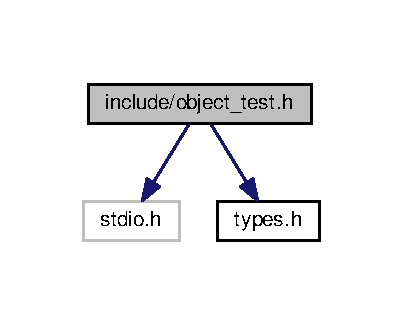
\includegraphics[width=194pt]{object__test_8h__incl}
\end{center}
\end{figure}
This graph shows which files directly or indirectly include this file\+:
\nopagebreak
\begin{figure}[H]
\begin{center}
\leavevmode
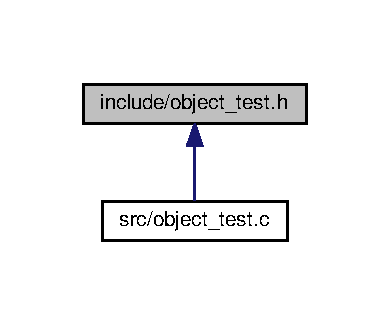
\includegraphics[width=187pt]{object__test_8h__dep__incl}
\end{center}
\end{figure}
\subsection*{Functions}
\begin{DoxyCompactItemize}
\item 
void \hyperlink{object__test_8h_a3836d69f92ce7149d56bafcaec83f516}{test1\+\_\+object\+\_\+create} ()
\item 
void \hyperlink{object__test_8h_add54ab5e33a1b0a93e9ddcf73591bd9f}{test2\+\_\+object\+\_\+create} ()
\item 
void \hyperlink{object__test_8h_aa88e9e9dab92ba9c58851d7a7a8415f0}{test1\+\_\+object\+\_\+get\+\_\+id} ()
\item 
void \hyperlink{object__test_8h_a1ff250f0f43297f57fcce1f3a6ae490b}{test2\+\_\+object\+\_\+get\+\_\+id} ()
\item 
void \hyperlink{object__test_8h_ac62fbd4db0970e9942aa900a3ee2bba4}{test1\+\_\+object\+\_\+get\+\_\+location} ()
\item 
void \hyperlink{object__test_8h_aa8e3d1f2c80097572d9a453737d8cd44}{test2\+\_\+object\+\_\+get\+\_\+location} ()
\item 
void \hyperlink{object__test_8h_a74e25ad653c4a32b9922fff8e4f916fd}{test1\+\_\+object\+\_\+set\+\_\+name} ()
\item 
void \hyperlink{object__test_8h_acf42b7e7be91ede243f2aaa56c4c9347}{test2\+\_\+object\+\_\+set\+\_\+name} ()
\item 
void \hyperlink{object__test_8h_ab40669b5d083b6484197d917fb6882b1}{test3\+\_\+object\+\_\+set\+\_\+name} ()
\item 
void \hyperlink{object__test_8h_ad2411bc3cc47c9905e63a3d9c561d369}{test1\+\_\+object\+\_\+get\+\_\+name} ()
\item 
void \hyperlink{object__test_8h_abdfafbc7b8588d3dcdb05fd2beb2397e}{test2\+\_\+object\+\_\+get\+\_\+name} ()
\item 
void \hyperlink{object__test_8h_a364b4f750a8a99ee3edd8eace90766da}{test1\+\_\+object\+\_\+set\+\_\+original\+\_\+description} ()
\item 
void \hyperlink{object__test_8h_a9f99963e555263ceef814fec86db4758}{test2\+\_\+object\+\_\+set\+\_\+original\+\_\+description} ()
\item 
void \hyperlink{object__test_8h_a61b511105851e73fb0bdaf0b7624370b}{test3\+\_\+object\+\_\+set\+\_\+original\+\_\+description} ()
\item 
void \hyperlink{object__test_8h_a239d56f1aad1ab85ca1ed897abc98052}{test1\+\_\+object\+\_\+get\+\_\+original\+\_\+description} ()
\item 
void \hyperlink{object__test_8h_af05f0ac1f5b56dd4cd7bedf9f5170cda}{test2\+\_\+object\+\_\+get\+\_\+original\+\_\+description} ()
\item 
void \hyperlink{object__test_8h_a6f19ebf6034115c2cdcc3c7bfea25964}{test1\+\_\+object\+\_\+set\+\_\+id} ()
\item 
void \hyperlink{object__test_8h_a1f0cfd69428a6cf954fe37c9c21f8cb3}{test2\+\_\+object\+\_\+set\+\_\+id} ()
\item 
void \hyperlink{object__test_8h_aeed901e95aa669185059c85183e68a24}{test1\+\_\+object\+\_\+set\+\_\+location} ()
\item 
void \hyperlink{object__test_8h_a728404dd60089346883f325281e88f5f}{test1\+\_\+object\+\_\+get\+\_\+prop\+\_\+\+Movable} ()
\item 
void \hyperlink{object__test_8h_a2b377a9a92a83b71996a961426983bca}{test2\+\_\+object\+\_\+get\+\_\+prop\+\_\+\+Movable} ()
\item 
void \hyperlink{object__test_8h_a3c03468ba567762d74f481366784209d}{test1\+\_\+object\+\_\+set\+\_\+prop\+\_\+\+Movable} ()
\item 
void \hyperlink{object__test_8h_a90b53ff8f01a8c2c233af68f0e59cb82}{test2\+\_\+object\+\_\+set\+\_\+prop\+\_\+\+Movable} ()
\item 
void \hyperlink{object__test_8h_a8764a4a50a115de3c998d6ae53e8020e}{test3\+\_\+object\+\_\+set\+\_\+prop\+\_\+\+Movable} ()
\item 
void \hyperlink{object__test_8h_acc9f038ee43213c830877448b76ccfdf}{test1\+\_\+object\+\_\+get\+\_\+prop\+\_\+\+Moved} ()
\item 
void \hyperlink{object__test_8h_a6c5952b03a7737bb7b44ae4a63a8ff0b}{test2\+\_\+object\+\_\+get\+\_\+prop\+\_\+\+Moved} ()
\item 
void \hyperlink{object__test_8h_a04878b6ba45bdf63222c309bd97f6b65}{test1\+\_\+object\+\_\+set\+\_\+prop\+\_\+\+Moved} ()
\item 
void \hyperlink{object__test_8h_ab357bb60ef2e7c2c32aa8f5bf96dc7f0}{test2\+\_\+object\+\_\+set\+\_\+prop\+\_\+\+Moved} ()
\item 
void \hyperlink{object__test_8h_a7789238ee5681e10b4d49e6e9f457d40}{test3\+\_\+object\+\_\+set\+\_\+prop\+\_\+\+Moved} ()
\item 
void \hyperlink{object__test_8h_a40fbfa7d317b726cb6d02b23deb3914f}{test1\+\_\+object\+\_\+get\+\_\+prop\+\_\+\+Illuminate} ()
\item 
void \hyperlink{object__test_8h_a689e4149735a5543014921c1579950a1}{test2\+\_\+object\+\_\+get\+\_\+prop\+\_\+\+Illuminate} ()
\item 
void \hyperlink{object__test_8h_a31cda74045f4f4a7f222705974dcf6de}{test1\+\_\+object\+\_\+set\+\_\+prop\+\_\+\+Illuminate} ()
\item 
void \hyperlink{object__test_8h_afb0a0cc9ade8ecc2c15ae9e5697e7211}{test2\+\_\+object\+\_\+set\+\_\+prop\+\_\+\+Illuminate} ()
\item 
void \hyperlink{object__test_8h_aa6e6c87c5a7f2d3552dd33d7a5f160cf}{test3\+\_\+object\+\_\+set\+\_\+prop\+\_\+\+Illuminate} ()
\item 
void \hyperlink{object__test_8h_a02608a9321ba268814c20a67e8fbce27}{test1\+\_\+object\+\_\+get\+\_\+prop\+\_\+\+Switched\+On} ()
\item 
void \hyperlink{object__test_8h_a1a023ed883d17c1fd32b924548306cf4}{test2\+\_\+object\+\_\+get\+\_\+prop\+\_\+\+Switched\+On} ()
\item 
void \hyperlink{object__test_8h_a3a0e24b6614bcad78cc6025165d4ab87}{test1\+\_\+object\+\_\+set\+\_\+prop\+\_\+\+Switched\+On} ()
\item 
void \hyperlink{object__test_8h_a08c0ca2b1c356924ca66dcbb15d9e970}{test2\+\_\+object\+\_\+set\+\_\+prop\+\_\+\+Switched\+On} ()
\item 
void \hyperlink{object__test_8h_a404400e229425a94d3ef8c5d826ece78}{test3\+\_\+object\+\_\+set\+\_\+prop\+\_\+\+Switched\+On} ()
\item 
void \hyperlink{object__test_8h_a27e7bae76305733c1a8036bf54a4ff34}{test1\+\_\+object\+\_\+get\+\_\+prop\+\_\+\+Open} ()
\item 
void \hyperlink{object__test_8h_a300abd0f902e0c5865a1351dbb6e65c4}{test2\+\_\+object\+\_\+get\+\_\+prop\+\_\+\+Open} ()
\item 
void \hyperlink{object__test_8h_a353246fe61194086aea1ca9f94008d9a}{test1\+\_\+object\+\_\+set\+\_\+prop\+\_\+\+Open} ()
\item 
void \hyperlink{object__test_8h_a197746b5a031a7d4fda89035f22050f8}{test2\+\_\+object\+\_\+set\+\_\+prop\+\_\+\+Open} ()
\item 
void \hyperlink{object__test_8h_ae36abb53263ed855bde4dc2f47195813}{test3\+\_\+object\+\_\+set\+\_\+prop\+\_\+\+Open} ()
\item 
void \hyperlink{object__test_8h_ad36938109a07bb264f1005fe9ff5b118}{test1\+\_\+object\+\_\+get\+\_\+original\+\_\+position} ()
\item 
void \hyperlink{object__test_8h_a90212ac853f2702bcf7f83046f493810}{test2\+\_\+object\+\_\+get\+\_\+original\+\_\+position} ()
\item 
void \hyperlink{object__test_8h_aaef8c81d135b0e5dcc9972bc04991c69}{test3\+\_\+object\+\_\+get\+\_\+original\+\_\+position} ()
\item 
void \hyperlink{object__test_8h_af3fb1a489226895731af93b686741849}{test1\+\_\+object\+\_\+set\+\_\+original\+\_\+position} ()
\item 
void \hyperlink{object__test_8h_a64501207ceb4c2481bb45a334c71668f}{test2\+\_\+object\+\_\+set\+\_\+original\+\_\+position} ()
\item 
void \hyperlink{object__test_8h_a1a521d43a34ab0744c551f547120b24e}{test3\+\_\+object\+\_\+set\+\_\+original\+\_\+position} ()
\item 
void \hyperlink{object__test_8h_ae1755561dd25ae3c9826c095b081e4bb}{test1\+\_\+object\+\_\+get\+\_\+prop\+\_\+\+Hidden} ()
\item 
void \hyperlink{object__test_8h_a2aa1c98ca2de8aab36614e37217a0907}{test2\+\_\+object\+\_\+get\+\_\+prop\+\_\+\+Hidden} ()
\item 
void \hyperlink{object__test_8h_a3684b2ca710956aa6e61d26236497b34}{test1\+\_\+object\+\_\+set\+\_\+prop\+\_\+\+Hidden} ()
\item 
void \hyperlink{object__test_8h_a5f05b32f7e951027ca0fca90da4ae89e}{test2\+\_\+object\+\_\+set\+\_\+prop\+\_\+\+Hidden} ()
\item 
void \hyperlink{object__test_8h_a83a9139598c0d1683c39a390ce4af8ad}{test3\+\_\+object\+\_\+set\+\_\+prop\+\_\+\+Hidden} ()
\end{DoxyCompactItemize}


\subsection{Detailed Description}
It declares the tests for the object module. 

\begin{DoxyAuthor}{Author}
Andrés Mena 
\end{DoxyAuthor}
\begin{DoxyVersion}{Version}
2.\+0 
\end{DoxyVersion}
\begin{DoxyDate}{Date}
01-\/04-\/2018 
\end{DoxyDate}
\begin{DoxyCopyright}{Copyright}
G\+NU Public License 
\end{DoxyCopyright}


\subsection{Function Documentation}
\index{object\+\_\+test.\+h@{object\+\_\+test.\+h}!test1\+\_\+object\+\_\+create@{test1\+\_\+object\+\_\+create}}
\index{test1\+\_\+object\+\_\+create@{test1\+\_\+object\+\_\+create}!object\+\_\+test.\+h@{object\+\_\+test.\+h}}
\subsubsection[{\texorpdfstring{test1\+\_\+object\+\_\+create()}{test1_object_create()}}]{\setlength{\rightskip}{0pt plus 5cm}void test1\+\_\+object\+\_\+create (
\begin{DoxyParamCaption}
{}
\end{DoxyParamCaption}
)}\hypertarget{object__test_8h_a3836d69f92ce7149d56bafcaec83f516}{}\label{object__test_8h_a3836d69f92ce7149d56bafcaec83f516}
\begin{DoxyRefDesc}{Test}
\item[\hyperlink{test__test000050}{Test}]Test object creation \end{DoxyRefDesc}
\begin{DoxyPrecond}{Precondition}
object ID 
\end{DoxyPrecond}
\begin{DoxyPostcond}{Postcondition}
Non N\+U\+LL pointer to object 
\end{DoxyPostcond}
\index{object\+\_\+test.\+h@{object\+\_\+test.\+h}!test1\+\_\+object\+\_\+get\+\_\+id@{test1\+\_\+object\+\_\+get\+\_\+id}}
\index{test1\+\_\+object\+\_\+get\+\_\+id@{test1\+\_\+object\+\_\+get\+\_\+id}!object\+\_\+test.\+h@{object\+\_\+test.\+h}}
\subsubsection[{\texorpdfstring{test1\+\_\+object\+\_\+get\+\_\+id()}{test1_object_get_id()}}]{\setlength{\rightskip}{0pt plus 5cm}void test1\+\_\+object\+\_\+get\+\_\+id (
\begin{DoxyParamCaption}
{}
\end{DoxyParamCaption}
)}\hypertarget{object__test_8h_aa88e9e9dab92ba9c58851d7a7a8415f0}{}\label{object__test_8h_aa88e9e9dab92ba9c58851d7a7a8415f0}
\begin{DoxyRefDesc}{Test}
\item[\hyperlink{test__test000052}{Test}]Test obtaining id of object \end{DoxyRefDesc}
\begin{DoxyPrecond}{Precondition}
Object pointer N\+U\+LL 
\end{DoxyPrecond}
\begin{DoxyPostcond}{Postcondition}
N\+O\+\_\+\+ID 
\end{DoxyPostcond}
\index{object\+\_\+test.\+h@{object\+\_\+test.\+h}!test1\+\_\+object\+\_\+get\+\_\+location@{test1\+\_\+object\+\_\+get\+\_\+location}}
\index{test1\+\_\+object\+\_\+get\+\_\+location@{test1\+\_\+object\+\_\+get\+\_\+location}!object\+\_\+test.\+h@{object\+\_\+test.\+h}}
\subsubsection[{\texorpdfstring{test1\+\_\+object\+\_\+get\+\_\+location()}{test1_object_get_location()}}]{\setlength{\rightskip}{0pt plus 5cm}void test1\+\_\+object\+\_\+get\+\_\+location (
\begin{DoxyParamCaption}
{}
\end{DoxyParamCaption}
)}\hypertarget{object__test_8h_ac62fbd4db0970e9942aa900a3ee2bba4}{}\label{object__test_8h_ac62fbd4db0970e9942aa900a3ee2bba4}
\begin{DoxyRefDesc}{Test}
\item[\hyperlink{test__test000054}{Test}]Test obtaining location of object \end{DoxyRefDesc}
\begin{DoxyPrecond}{Precondition}
Object pointer N\+U\+LL 
\end{DoxyPrecond}
\begin{DoxyPostcond}{Postcondition}
N\+O\+\_\+\+ID 
\end{DoxyPostcond}
\index{object\+\_\+test.\+h@{object\+\_\+test.\+h}!test1\+\_\+object\+\_\+get\+\_\+name@{test1\+\_\+object\+\_\+get\+\_\+name}}
\index{test1\+\_\+object\+\_\+get\+\_\+name@{test1\+\_\+object\+\_\+get\+\_\+name}!object\+\_\+test.\+h@{object\+\_\+test.\+h}}
\subsubsection[{\texorpdfstring{test1\+\_\+object\+\_\+get\+\_\+name()}{test1_object_get_name()}}]{\setlength{\rightskip}{0pt plus 5cm}void test1\+\_\+object\+\_\+get\+\_\+name (
\begin{DoxyParamCaption}
{}
\end{DoxyParamCaption}
)}\hypertarget{object__test_8h_ad2411bc3cc47c9905e63a3d9c561d369}{}\label{object__test_8h_ad2411bc3cc47c9905e63a3d9c561d369}
\begin{DoxyRefDesc}{Test}
\item[\hyperlink{test__test000059}{Test}]Test function for object\+\_\+name obtaining \end{DoxyRefDesc}
\begin{DoxyPrecond}{Precondition}
Object pointer 
\end{DoxyPrecond}
\begin{DoxyPostcond}{Postcondition}
string of characters (previously added) 
\end{DoxyPostcond}
\index{object\+\_\+test.\+h@{object\+\_\+test.\+h}!test1\+\_\+object\+\_\+get\+\_\+original\+\_\+description@{test1\+\_\+object\+\_\+get\+\_\+original\+\_\+description}}
\index{test1\+\_\+object\+\_\+get\+\_\+original\+\_\+description@{test1\+\_\+object\+\_\+get\+\_\+original\+\_\+description}!object\+\_\+test.\+h@{object\+\_\+test.\+h}}
\subsubsection[{\texorpdfstring{test1\+\_\+object\+\_\+get\+\_\+original\+\_\+description()}{test1_object_get_original_description()}}]{\setlength{\rightskip}{0pt plus 5cm}void test1\+\_\+object\+\_\+get\+\_\+original\+\_\+description (
\begin{DoxyParamCaption}
{}
\end{DoxyParamCaption}
)}\hypertarget{object__test_8h_a239d56f1aad1ab85ca1ed897abc98052}{}\label{object__test_8h_a239d56f1aad1ab85ca1ed897abc98052}
\begin{DoxyRefDesc}{Test}
\item[\hyperlink{test__test000064}{Test}]Test function for description of object obtaining \end{DoxyRefDesc}
\begin{DoxyPrecond}{Precondition}
Object pointer 
\end{DoxyPrecond}
\begin{DoxyPostcond}{Postcondition}
String with name 
\end{DoxyPostcond}
\index{object\+\_\+test.\+h@{object\+\_\+test.\+h}!test1\+\_\+object\+\_\+get\+\_\+original\+\_\+position@{test1\+\_\+object\+\_\+get\+\_\+original\+\_\+position}}
\index{test1\+\_\+object\+\_\+get\+\_\+original\+\_\+position@{test1\+\_\+object\+\_\+get\+\_\+original\+\_\+position}!object\+\_\+test.\+h@{object\+\_\+test.\+h}}
\subsubsection[{\texorpdfstring{test1\+\_\+object\+\_\+get\+\_\+original\+\_\+position()}{test1_object_get_original_position()}}]{\setlength{\rightskip}{0pt plus 5cm}void test1\+\_\+object\+\_\+get\+\_\+original\+\_\+position (
\begin{DoxyParamCaption}
{}
\end{DoxyParamCaption}
)}\hypertarget{object__test_8h_ad36938109a07bb264f1005fe9ff5b118}{}\label{object__test_8h_ad36938109a07bb264f1005fe9ff5b118}
\begin{DoxyRefDesc}{Test}
\item[\hyperlink{test__test000094}{Test}]Test getting original position of object \end{DoxyRefDesc}
\begin{DoxyPrecond}{Precondition}
Object pointer 
\end{DoxyPrecond}
\begin{DoxyPostcond}{Postcondition}
N\+O\+\_\+\+ID 
\end{DoxyPostcond}
\index{object\+\_\+test.\+h@{object\+\_\+test.\+h}!test1\+\_\+object\+\_\+get\+\_\+prop\+\_\+\+Hidden@{test1\+\_\+object\+\_\+get\+\_\+prop\+\_\+\+Hidden}}
\index{test1\+\_\+object\+\_\+get\+\_\+prop\+\_\+\+Hidden@{test1\+\_\+object\+\_\+get\+\_\+prop\+\_\+\+Hidden}!object\+\_\+test.\+h@{object\+\_\+test.\+h}}
\subsubsection[{\texorpdfstring{test1\+\_\+object\+\_\+get\+\_\+prop\+\_\+\+Hidden()}{test1_object_get_prop_Hidden()}}]{\setlength{\rightskip}{0pt plus 5cm}void test1\+\_\+object\+\_\+get\+\_\+prop\+\_\+\+Hidden (
\begin{DoxyParamCaption}
{}
\end{DoxyParamCaption}
)}\hypertarget{object__test_8h_ae1755561dd25ae3c9826c095b081e4bb}{}\label{object__test_8h_ae1755561dd25ae3c9826c095b081e4bb}
\begin{DoxyRefDesc}{Test}
\item[\hyperlink{test__test000100}{Test}]Test obtaining property Hidden of object \end{DoxyRefDesc}
\begin{DoxyPrecond}{Precondition}
Object pointer 
\end{DoxyPrecond}
\begin{DoxyPostcond}{Postcondition}
F\+A\+L\+SE property 
\end{DoxyPostcond}
\index{object\+\_\+test.\+h@{object\+\_\+test.\+h}!test1\+\_\+object\+\_\+get\+\_\+prop\+\_\+\+Illuminate@{test1\+\_\+object\+\_\+get\+\_\+prop\+\_\+\+Illuminate}}
\index{test1\+\_\+object\+\_\+get\+\_\+prop\+\_\+\+Illuminate@{test1\+\_\+object\+\_\+get\+\_\+prop\+\_\+\+Illuminate}!object\+\_\+test.\+h@{object\+\_\+test.\+h}}
\subsubsection[{\texorpdfstring{test1\+\_\+object\+\_\+get\+\_\+prop\+\_\+\+Illuminate()}{test1_object_get_prop_Illuminate()}}]{\setlength{\rightskip}{0pt plus 5cm}void test1\+\_\+object\+\_\+get\+\_\+prop\+\_\+\+Illuminate (
\begin{DoxyParamCaption}
{}
\end{DoxyParamCaption}
)}\hypertarget{object__test_8h_a40fbfa7d317b726cb6d02b23deb3914f}{}\label{object__test_8h_a40fbfa7d317b726cb6d02b23deb3914f}
\begin{DoxyRefDesc}{Test}
\item[\hyperlink{test__test000079}{Test}]Test obtaining property illuminate of object \end{DoxyRefDesc}
\begin{DoxyPrecond}{Precondition}
Object pointer 
\end{DoxyPrecond}
\begin{DoxyPostcond}{Postcondition}
F\+A\+L\+SE property 
\end{DoxyPostcond}
\index{object\+\_\+test.\+h@{object\+\_\+test.\+h}!test1\+\_\+object\+\_\+get\+\_\+prop\+\_\+\+Movable@{test1\+\_\+object\+\_\+get\+\_\+prop\+\_\+\+Movable}}
\index{test1\+\_\+object\+\_\+get\+\_\+prop\+\_\+\+Movable@{test1\+\_\+object\+\_\+get\+\_\+prop\+\_\+\+Movable}!object\+\_\+test.\+h@{object\+\_\+test.\+h}}
\subsubsection[{\texorpdfstring{test1\+\_\+object\+\_\+get\+\_\+prop\+\_\+\+Movable()}{test1_object_get_prop_Movable()}}]{\setlength{\rightskip}{0pt plus 5cm}void test1\+\_\+object\+\_\+get\+\_\+prop\+\_\+\+Movable (
\begin{DoxyParamCaption}
{}
\end{DoxyParamCaption}
)}\hypertarget{object__test_8h_a728404dd60089346883f325281e88f5f}{}\label{object__test_8h_a728404dd60089346883f325281e88f5f}
\begin{DoxyRefDesc}{Test}
\item[\hyperlink{test__test000069}{Test}]Test obtaining property movable of object \end{DoxyRefDesc}
\begin{DoxyPrecond}{Precondition}
Object pointer 
\end{DoxyPrecond}
\begin{DoxyPostcond}{Postcondition}
F\+A\+L\+SE property 
\end{DoxyPostcond}
\index{object\+\_\+test.\+h@{object\+\_\+test.\+h}!test1\+\_\+object\+\_\+get\+\_\+prop\+\_\+\+Moved@{test1\+\_\+object\+\_\+get\+\_\+prop\+\_\+\+Moved}}
\index{test1\+\_\+object\+\_\+get\+\_\+prop\+\_\+\+Moved@{test1\+\_\+object\+\_\+get\+\_\+prop\+\_\+\+Moved}!object\+\_\+test.\+h@{object\+\_\+test.\+h}}
\subsubsection[{\texorpdfstring{test1\+\_\+object\+\_\+get\+\_\+prop\+\_\+\+Moved()}{test1_object_get_prop_Moved()}}]{\setlength{\rightskip}{0pt plus 5cm}void test1\+\_\+object\+\_\+get\+\_\+prop\+\_\+\+Moved (
\begin{DoxyParamCaption}
{}
\end{DoxyParamCaption}
)}\hypertarget{object__test_8h_acc9f038ee43213c830877448b76ccfdf}{}\label{object__test_8h_acc9f038ee43213c830877448b76ccfdf}
\begin{DoxyRefDesc}{Test}
\item[\hyperlink{test__test000074}{Test}]Test obtaining property moved of object \end{DoxyRefDesc}
\begin{DoxyPrecond}{Precondition}
Object pointer 
\end{DoxyPrecond}
\begin{DoxyPostcond}{Postcondition}
F\+A\+L\+SE property 
\end{DoxyPostcond}
\index{object\+\_\+test.\+h@{object\+\_\+test.\+h}!test1\+\_\+object\+\_\+get\+\_\+prop\+\_\+\+Open@{test1\+\_\+object\+\_\+get\+\_\+prop\+\_\+\+Open}}
\index{test1\+\_\+object\+\_\+get\+\_\+prop\+\_\+\+Open@{test1\+\_\+object\+\_\+get\+\_\+prop\+\_\+\+Open}!object\+\_\+test.\+h@{object\+\_\+test.\+h}}
\subsubsection[{\texorpdfstring{test1\+\_\+object\+\_\+get\+\_\+prop\+\_\+\+Open()}{test1_object_get_prop_Open()}}]{\setlength{\rightskip}{0pt plus 5cm}void test1\+\_\+object\+\_\+get\+\_\+prop\+\_\+\+Open (
\begin{DoxyParamCaption}
{}
\end{DoxyParamCaption}
)}\hypertarget{object__test_8h_a27e7bae76305733c1a8036bf54a4ff34}{}\label{object__test_8h_a27e7bae76305733c1a8036bf54a4ff34}
\begin{DoxyRefDesc}{Test}
\item[\hyperlink{test__test000089}{Test}]Test getting property open of object \end{DoxyRefDesc}
\begin{DoxyPrecond}{Precondition}
Object pointer 
\end{DoxyPrecond}
\begin{DoxyPostcond}{Postcondition}
N\+O\+\_\+\+ID 
\end{DoxyPostcond}
\index{object\+\_\+test.\+h@{object\+\_\+test.\+h}!test1\+\_\+object\+\_\+get\+\_\+prop\+\_\+\+Switched\+On@{test1\+\_\+object\+\_\+get\+\_\+prop\+\_\+\+Switched\+On}}
\index{test1\+\_\+object\+\_\+get\+\_\+prop\+\_\+\+Switched\+On@{test1\+\_\+object\+\_\+get\+\_\+prop\+\_\+\+Switched\+On}!object\+\_\+test.\+h@{object\+\_\+test.\+h}}
\subsubsection[{\texorpdfstring{test1\+\_\+object\+\_\+get\+\_\+prop\+\_\+\+Switched\+On()}{test1_object_get_prop_SwitchedOn()}}]{\setlength{\rightskip}{0pt plus 5cm}void test1\+\_\+object\+\_\+get\+\_\+prop\+\_\+\+Switched\+On (
\begin{DoxyParamCaption}
{}
\end{DoxyParamCaption}
)}\hypertarget{object__test_8h_a02608a9321ba268814c20a67e8fbce27}{}\label{object__test_8h_a02608a9321ba268814c20a67e8fbce27}
\begin{DoxyRefDesc}{Test}
\item[\hyperlink{test__test000084}{Test}]Test obtaining property switchedon of object \end{DoxyRefDesc}
\begin{DoxyPrecond}{Precondition}
Object pointer 
\end{DoxyPrecond}
\begin{DoxyPostcond}{Postcondition}
F\+A\+L\+SE property 
\end{DoxyPostcond}
\index{object\+\_\+test.\+h@{object\+\_\+test.\+h}!test1\+\_\+object\+\_\+set\+\_\+id@{test1\+\_\+object\+\_\+set\+\_\+id}}
\index{test1\+\_\+object\+\_\+set\+\_\+id@{test1\+\_\+object\+\_\+set\+\_\+id}!object\+\_\+test.\+h@{object\+\_\+test.\+h}}
\subsubsection[{\texorpdfstring{test1\+\_\+object\+\_\+set\+\_\+id()}{test1_object_set_id()}}]{\setlength{\rightskip}{0pt plus 5cm}void test1\+\_\+object\+\_\+set\+\_\+id (
\begin{DoxyParamCaption}
{}
\end{DoxyParamCaption}
)}\hypertarget{object__test_8h_a6f19ebf6034115c2cdcc3c7bfea25964}{}\label{object__test_8h_a6f19ebf6034115c2cdcc3c7bfea25964}
\begin{DoxyRefDesc}{Test}
\item[\hyperlink{test__test000066}{Test}]Test obtaining id of object \end{DoxyRefDesc}
\begin{DoxyPrecond}{Precondition}
Object pointer (with object id) 
\end{DoxyPrecond}
\begin{DoxyPostcond}{Postcondition}
Id of object 
\end{DoxyPostcond}
\index{object\+\_\+test.\+h@{object\+\_\+test.\+h}!test1\+\_\+object\+\_\+set\+\_\+location@{test1\+\_\+object\+\_\+set\+\_\+location}}
\index{test1\+\_\+object\+\_\+set\+\_\+location@{test1\+\_\+object\+\_\+set\+\_\+location}!object\+\_\+test.\+h@{object\+\_\+test.\+h}}
\subsubsection[{\texorpdfstring{test1\+\_\+object\+\_\+set\+\_\+location()}{test1_object_set_location()}}]{\setlength{\rightskip}{0pt plus 5cm}void test1\+\_\+object\+\_\+set\+\_\+location (
\begin{DoxyParamCaption}
{}
\end{DoxyParamCaption}
)}\hypertarget{object__test_8h_aeed901e95aa669185059c85183e68a24}{}\label{object__test_8h_aeed901e95aa669185059c85183e68a24}
\begin{DoxyRefDesc}{Test}
\item[\hyperlink{test__test000068}{Test}]Test obtaining location of object \end{DoxyRefDesc}
\begin{DoxyPrecond}{Precondition}
Object pointer with object added 
\end{DoxyPrecond}
\begin{DoxyPostcond}{Postcondition}
object location == location sent 
\end{DoxyPostcond}
\index{object\+\_\+test.\+h@{object\+\_\+test.\+h}!test1\+\_\+object\+\_\+set\+\_\+name@{test1\+\_\+object\+\_\+set\+\_\+name}}
\index{test1\+\_\+object\+\_\+set\+\_\+name@{test1\+\_\+object\+\_\+set\+\_\+name}!object\+\_\+test.\+h@{object\+\_\+test.\+h}}
\subsubsection[{\texorpdfstring{test1\+\_\+object\+\_\+set\+\_\+name()}{test1_object_set_name()}}]{\setlength{\rightskip}{0pt plus 5cm}void test1\+\_\+object\+\_\+set\+\_\+name (
\begin{DoxyParamCaption}
{}
\end{DoxyParamCaption}
)}\hypertarget{object__test_8h_a74e25ad653c4a32b9922fff8e4f916fd}{}\label{object__test_8h_a74e25ad653c4a32b9922fff8e4f916fd}
\begin{DoxyRefDesc}{Test}
\item[\hyperlink{test__test000056}{Test}]Test function object\+\_\+name setting \end{DoxyRefDesc}
\begin{DoxyPrecond}{Precondition}
String with space name and Object pointer 
\end{DoxyPrecond}
\begin{DoxyPostcond}{Postcondition}
Ouput==OK 
\end{DoxyPostcond}
\index{object\+\_\+test.\+h@{object\+\_\+test.\+h}!test1\+\_\+object\+\_\+set\+\_\+original\+\_\+description@{test1\+\_\+object\+\_\+set\+\_\+original\+\_\+description}}
\index{test1\+\_\+object\+\_\+set\+\_\+original\+\_\+description@{test1\+\_\+object\+\_\+set\+\_\+original\+\_\+description}!object\+\_\+test.\+h@{object\+\_\+test.\+h}}
\subsubsection[{\texorpdfstring{test1\+\_\+object\+\_\+set\+\_\+original\+\_\+description()}{test1_object_set_original_description()}}]{\setlength{\rightskip}{0pt plus 5cm}void test1\+\_\+object\+\_\+set\+\_\+original\+\_\+description (
\begin{DoxyParamCaption}
{}
\end{DoxyParamCaption}
)}\hypertarget{object__test_8h_a364b4f750a8a99ee3edd8eace90766da}{}\label{object__test_8h_a364b4f750a8a99ee3edd8eace90766da}
\begin{DoxyRefDesc}{Test}
\item[\hyperlink{test__test000061}{Test}]Test function for description of object setting \end{DoxyRefDesc}
\begin{DoxyPrecond}{Precondition}
String of characters and Object pointer 
\end{DoxyPrecond}
\begin{DoxyPostcond}{Postcondition}
S\+T\+A\+T\+US=OK 
\end{DoxyPostcond}
\index{object\+\_\+test.\+h@{object\+\_\+test.\+h}!test1\+\_\+object\+\_\+set\+\_\+original\+\_\+position@{test1\+\_\+object\+\_\+set\+\_\+original\+\_\+position}}
\index{test1\+\_\+object\+\_\+set\+\_\+original\+\_\+position@{test1\+\_\+object\+\_\+set\+\_\+original\+\_\+position}!object\+\_\+test.\+h@{object\+\_\+test.\+h}}
\subsubsection[{\texorpdfstring{test1\+\_\+object\+\_\+set\+\_\+original\+\_\+position()}{test1_object_set_original_position()}}]{\setlength{\rightskip}{0pt plus 5cm}void test1\+\_\+object\+\_\+set\+\_\+original\+\_\+position (
\begin{DoxyParamCaption}
{}
\end{DoxyParamCaption}
)}\hypertarget{object__test_8h_af3fb1a489226895731af93b686741849}{}\label{object__test_8h_af3fb1a489226895731af93b686741849}
\begin{DoxyRefDesc}{Test}
\item[\hyperlink{test__test000097}{Test}]Test setting original position of object \end{DoxyRefDesc}
\begin{DoxyPrecond}{Precondition}
Object pointer with a position 
\end{DoxyPrecond}
\begin{DoxyPostcond}{Postcondition}
Position introduced previously 
\end{DoxyPostcond}
\index{object\+\_\+test.\+h@{object\+\_\+test.\+h}!test1\+\_\+object\+\_\+set\+\_\+prop\+\_\+\+Hidden@{test1\+\_\+object\+\_\+set\+\_\+prop\+\_\+\+Hidden}}
\index{test1\+\_\+object\+\_\+set\+\_\+prop\+\_\+\+Hidden@{test1\+\_\+object\+\_\+set\+\_\+prop\+\_\+\+Hidden}!object\+\_\+test.\+h@{object\+\_\+test.\+h}}
\subsubsection[{\texorpdfstring{test1\+\_\+object\+\_\+set\+\_\+prop\+\_\+\+Hidden()}{test1_object_set_prop_Hidden()}}]{\setlength{\rightskip}{0pt plus 5cm}void test1\+\_\+object\+\_\+set\+\_\+prop\+\_\+\+Hidden (
\begin{DoxyParamCaption}
{}
\end{DoxyParamCaption}
)}\hypertarget{object__test_8h_a3684b2ca710956aa6e61d26236497b34}{}\label{object__test_8h_a3684b2ca710956aa6e61d26236497b34}
\begin{DoxyRefDesc}{Test}
\item[\hyperlink{test__test000102}{Test}]Test setting property Hidden of object \end{DoxyRefDesc}
\begin{DoxyPrecond}{Precondition}
Object pointer and T\+R\+UE boolean 
\end{DoxyPrecond}
\begin{DoxyPostcond}{Postcondition}
T\+R\+UE property 
\end{DoxyPostcond}
\index{object\+\_\+test.\+h@{object\+\_\+test.\+h}!test1\+\_\+object\+\_\+set\+\_\+prop\+\_\+\+Illuminate@{test1\+\_\+object\+\_\+set\+\_\+prop\+\_\+\+Illuminate}}
\index{test1\+\_\+object\+\_\+set\+\_\+prop\+\_\+\+Illuminate@{test1\+\_\+object\+\_\+set\+\_\+prop\+\_\+\+Illuminate}!object\+\_\+test.\+h@{object\+\_\+test.\+h}}
\subsubsection[{\texorpdfstring{test1\+\_\+object\+\_\+set\+\_\+prop\+\_\+\+Illuminate()}{test1_object_set_prop_Illuminate()}}]{\setlength{\rightskip}{0pt plus 5cm}void test1\+\_\+object\+\_\+set\+\_\+prop\+\_\+\+Illuminate (
\begin{DoxyParamCaption}
{}
\end{DoxyParamCaption}
)}\hypertarget{object__test_8h_a31cda74045f4f4a7f222705974dcf6de}{}\label{object__test_8h_a31cda74045f4f4a7f222705974dcf6de}
\begin{DoxyRefDesc}{Test}
\item[\hyperlink{test__test000081}{Test}]Test setting property illuminate of object \end{DoxyRefDesc}
\begin{DoxyPrecond}{Precondition}
Object pointer and T\+R\+UE boolean 
\end{DoxyPrecond}
\begin{DoxyPostcond}{Postcondition}
T\+R\+UE property 
\end{DoxyPostcond}
\index{object\+\_\+test.\+h@{object\+\_\+test.\+h}!test1\+\_\+object\+\_\+set\+\_\+prop\+\_\+\+Movable@{test1\+\_\+object\+\_\+set\+\_\+prop\+\_\+\+Movable}}
\index{test1\+\_\+object\+\_\+set\+\_\+prop\+\_\+\+Movable@{test1\+\_\+object\+\_\+set\+\_\+prop\+\_\+\+Movable}!object\+\_\+test.\+h@{object\+\_\+test.\+h}}
\subsubsection[{\texorpdfstring{test1\+\_\+object\+\_\+set\+\_\+prop\+\_\+\+Movable()}{test1_object_set_prop_Movable()}}]{\setlength{\rightskip}{0pt plus 5cm}void test1\+\_\+object\+\_\+set\+\_\+prop\+\_\+\+Movable (
\begin{DoxyParamCaption}
{}
\end{DoxyParamCaption}
)}\hypertarget{object__test_8h_a3c03468ba567762d74f481366784209d}{}\label{object__test_8h_a3c03468ba567762d74f481366784209d}
\begin{DoxyRefDesc}{Test}
\item[\hyperlink{test__test000071}{Test}]Test setting property movable of object \end{DoxyRefDesc}
\begin{DoxyPrecond}{Precondition}
Object pointer and T\+R\+UE boolean 
\end{DoxyPrecond}
\begin{DoxyPostcond}{Postcondition}
T\+R\+UE property 
\end{DoxyPostcond}
\index{object\+\_\+test.\+h@{object\+\_\+test.\+h}!test1\+\_\+object\+\_\+set\+\_\+prop\+\_\+\+Moved@{test1\+\_\+object\+\_\+set\+\_\+prop\+\_\+\+Moved}}
\index{test1\+\_\+object\+\_\+set\+\_\+prop\+\_\+\+Moved@{test1\+\_\+object\+\_\+set\+\_\+prop\+\_\+\+Moved}!object\+\_\+test.\+h@{object\+\_\+test.\+h}}
\subsubsection[{\texorpdfstring{test1\+\_\+object\+\_\+set\+\_\+prop\+\_\+\+Moved()}{test1_object_set_prop_Moved()}}]{\setlength{\rightskip}{0pt plus 5cm}void test1\+\_\+object\+\_\+set\+\_\+prop\+\_\+\+Moved (
\begin{DoxyParamCaption}
{}
\end{DoxyParamCaption}
)}\hypertarget{object__test_8h_a04878b6ba45bdf63222c309bd97f6b65}{}\label{object__test_8h_a04878b6ba45bdf63222c309bd97f6b65}
\begin{DoxyRefDesc}{Test}
\item[\hyperlink{test__test000076}{Test}]Test setting property moved of object \end{DoxyRefDesc}
\begin{DoxyPrecond}{Precondition}
Object pointer and T\+R\+UE boolean 
\end{DoxyPrecond}
\begin{DoxyPostcond}{Postcondition}
T\+R\+UE property 
\end{DoxyPostcond}
\index{object\+\_\+test.\+h@{object\+\_\+test.\+h}!test1\+\_\+object\+\_\+set\+\_\+prop\+\_\+\+Open@{test1\+\_\+object\+\_\+set\+\_\+prop\+\_\+\+Open}}
\index{test1\+\_\+object\+\_\+set\+\_\+prop\+\_\+\+Open@{test1\+\_\+object\+\_\+set\+\_\+prop\+\_\+\+Open}!object\+\_\+test.\+h@{object\+\_\+test.\+h}}
\subsubsection[{\texorpdfstring{test1\+\_\+object\+\_\+set\+\_\+prop\+\_\+\+Open()}{test1_object_set_prop_Open()}}]{\setlength{\rightskip}{0pt plus 5cm}void test1\+\_\+object\+\_\+set\+\_\+prop\+\_\+\+Open (
\begin{DoxyParamCaption}
{}
\end{DoxyParamCaption}
)}\hypertarget{object__test_8h_a353246fe61194086aea1ca9f94008d9a}{}\label{object__test_8h_a353246fe61194086aea1ca9f94008d9a}
\begin{DoxyRefDesc}{Test}
\item[\hyperlink{test__test000091}{Test}]Test setting property open of object \end{DoxyRefDesc}
\begin{DoxyPrecond}{Precondition}
Object pointer and ID 
\end{DoxyPrecond}
\begin{DoxyPostcond}{Postcondition}
ID previously introduced 
\end{DoxyPostcond}
\index{object\+\_\+test.\+h@{object\+\_\+test.\+h}!test1\+\_\+object\+\_\+set\+\_\+prop\+\_\+\+Switched\+On@{test1\+\_\+object\+\_\+set\+\_\+prop\+\_\+\+Switched\+On}}
\index{test1\+\_\+object\+\_\+set\+\_\+prop\+\_\+\+Switched\+On@{test1\+\_\+object\+\_\+set\+\_\+prop\+\_\+\+Switched\+On}!object\+\_\+test.\+h@{object\+\_\+test.\+h}}
\subsubsection[{\texorpdfstring{test1\+\_\+object\+\_\+set\+\_\+prop\+\_\+\+Switched\+On()}{test1_object_set_prop_SwitchedOn()}}]{\setlength{\rightskip}{0pt plus 5cm}void test1\+\_\+object\+\_\+set\+\_\+prop\+\_\+\+Switched\+On (
\begin{DoxyParamCaption}
{}
\end{DoxyParamCaption}
)}\hypertarget{object__test_8h_a3a0e24b6614bcad78cc6025165d4ab87}{}\label{object__test_8h_a3a0e24b6614bcad78cc6025165d4ab87}
\begin{DoxyRefDesc}{Test}
\item[\hyperlink{test__test000086}{Test}]Test setting property switchedon of object \end{DoxyRefDesc}
\begin{DoxyPrecond}{Precondition}
Object pointer and T\+R\+UE boolean 
\end{DoxyPrecond}
\begin{DoxyPostcond}{Postcondition}
T\+R\+UE property 
\end{DoxyPostcond}
\index{object\+\_\+test.\+h@{object\+\_\+test.\+h}!test2\+\_\+object\+\_\+create@{test2\+\_\+object\+\_\+create}}
\index{test2\+\_\+object\+\_\+create@{test2\+\_\+object\+\_\+create}!object\+\_\+test.\+h@{object\+\_\+test.\+h}}
\subsubsection[{\texorpdfstring{test2\+\_\+object\+\_\+create()}{test2_object_create()}}]{\setlength{\rightskip}{0pt plus 5cm}void test2\+\_\+object\+\_\+create (
\begin{DoxyParamCaption}
{}
\end{DoxyParamCaption}
)}\hypertarget{object__test_8h_add54ab5e33a1b0a93e9ddcf73591bd9f}{}\label{object__test_8h_add54ab5e33a1b0a93e9ddcf73591bd9f}
\begin{DoxyRefDesc}{Test}
\item[\hyperlink{test__test000051}{Test}]Test object creation \end{DoxyRefDesc}
\begin{DoxyPrecond}{Precondition}
object ID 
\end{DoxyPrecond}
\begin{DoxyPostcond}{Postcondition}
Object\+\_\+\+ID == Supplied Object Id 
\end{DoxyPostcond}
\index{object\+\_\+test.\+h@{object\+\_\+test.\+h}!test2\+\_\+object\+\_\+get\+\_\+id@{test2\+\_\+object\+\_\+get\+\_\+id}}
\index{test2\+\_\+object\+\_\+get\+\_\+id@{test2\+\_\+object\+\_\+get\+\_\+id}!object\+\_\+test.\+h@{object\+\_\+test.\+h}}
\subsubsection[{\texorpdfstring{test2\+\_\+object\+\_\+get\+\_\+id()}{test2_object_get_id()}}]{\setlength{\rightskip}{0pt plus 5cm}void test2\+\_\+object\+\_\+get\+\_\+id (
\begin{DoxyParamCaption}
{}
\end{DoxyParamCaption}
)}\hypertarget{object__test_8h_a1ff250f0f43297f57fcce1f3a6ae490b}{}\label{object__test_8h_a1ff250f0f43297f57fcce1f3a6ae490b}
\begin{DoxyRefDesc}{Test}
\item[\hyperlink{test__test000053}{Test}]Test obtaining id of object \end{DoxyRefDesc}
\begin{DoxyPrecond}{Precondition}
Object pointer 
\end{DoxyPrecond}
\begin{DoxyPostcond}{Postcondition}
id of the object 
\end{DoxyPostcond}
\index{object\+\_\+test.\+h@{object\+\_\+test.\+h}!test2\+\_\+object\+\_\+get\+\_\+location@{test2\+\_\+object\+\_\+get\+\_\+location}}
\index{test2\+\_\+object\+\_\+get\+\_\+location@{test2\+\_\+object\+\_\+get\+\_\+location}!object\+\_\+test.\+h@{object\+\_\+test.\+h}}
\subsubsection[{\texorpdfstring{test2\+\_\+object\+\_\+get\+\_\+location()}{test2_object_get_location()}}]{\setlength{\rightskip}{0pt plus 5cm}void test2\+\_\+object\+\_\+get\+\_\+location (
\begin{DoxyParamCaption}
{}
\end{DoxyParamCaption}
)}\hypertarget{object__test_8h_aa8e3d1f2c80097572d9a453737d8cd44}{}\label{object__test_8h_aa8e3d1f2c80097572d9a453737d8cd44}
\begin{DoxyRefDesc}{Test}
\item[\hyperlink{test__test000055}{Test}]Test obtaining location of object \end{DoxyRefDesc}
\begin{DoxyPrecond}{Precondition}
Object pointer 
\end{DoxyPrecond}
\begin{DoxyPostcond}{Postcondition}
id of object previously added 
\end{DoxyPostcond}
\index{object\+\_\+test.\+h@{object\+\_\+test.\+h}!test2\+\_\+object\+\_\+get\+\_\+name@{test2\+\_\+object\+\_\+get\+\_\+name}}
\index{test2\+\_\+object\+\_\+get\+\_\+name@{test2\+\_\+object\+\_\+get\+\_\+name}!object\+\_\+test.\+h@{object\+\_\+test.\+h}}
\subsubsection[{\texorpdfstring{test2\+\_\+object\+\_\+get\+\_\+name()}{test2_object_get_name()}}]{\setlength{\rightskip}{0pt plus 5cm}void test2\+\_\+object\+\_\+get\+\_\+name (
\begin{DoxyParamCaption}
{}
\end{DoxyParamCaption}
)}\hypertarget{object__test_8h_abdfafbc7b8588d3dcdb05fd2beb2397e}{}\label{object__test_8h_abdfafbc7b8588d3dcdb05fd2beb2397e}
\begin{DoxyRefDesc}{Test}
\item[\hyperlink{test__test000060}{Test}]Test function for object\+\_\+name obtaining \end{DoxyRefDesc}
\begin{DoxyPrecond}{Precondition}
Object pointer N\+U\+LL 
\end{DoxyPrecond}
\begin{DoxyPostcond}{Postcondition}
N\+U\+LL 
\end{DoxyPostcond}
\index{object\+\_\+test.\+h@{object\+\_\+test.\+h}!test2\+\_\+object\+\_\+get\+\_\+original\+\_\+description@{test2\+\_\+object\+\_\+get\+\_\+original\+\_\+description}}
\index{test2\+\_\+object\+\_\+get\+\_\+original\+\_\+description@{test2\+\_\+object\+\_\+get\+\_\+original\+\_\+description}!object\+\_\+test.\+h@{object\+\_\+test.\+h}}
\subsubsection[{\texorpdfstring{test2\+\_\+object\+\_\+get\+\_\+original\+\_\+description()}{test2_object_get_original_description()}}]{\setlength{\rightskip}{0pt plus 5cm}void test2\+\_\+object\+\_\+get\+\_\+original\+\_\+description (
\begin{DoxyParamCaption}
{}
\end{DoxyParamCaption}
)}\hypertarget{object__test_8h_af05f0ac1f5b56dd4cd7bedf9f5170cda}{}\label{object__test_8h_af05f0ac1f5b56dd4cd7bedf9f5170cda}
\begin{DoxyRefDesc}{Test}
\item[\hyperlink{test__test000065}{Test}]Test function for description of object obtaining \end{DoxyRefDesc}
\begin{DoxyPrecond}{Precondition}
Object pointer N\+U\+LL 
\end{DoxyPrecond}
\begin{DoxyPostcond}{Postcondition}
N\+U\+LL 
\end{DoxyPostcond}
\index{object\+\_\+test.\+h@{object\+\_\+test.\+h}!test2\+\_\+object\+\_\+get\+\_\+original\+\_\+position@{test2\+\_\+object\+\_\+get\+\_\+original\+\_\+position}}
\index{test2\+\_\+object\+\_\+get\+\_\+original\+\_\+position@{test2\+\_\+object\+\_\+get\+\_\+original\+\_\+position}!object\+\_\+test.\+h@{object\+\_\+test.\+h}}
\subsubsection[{\texorpdfstring{test2\+\_\+object\+\_\+get\+\_\+original\+\_\+position()}{test2_object_get_original_position()}}]{\setlength{\rightskip}{0pt plus 5cm}void test2\+\_\+object\+\_\+get\+\_\+original\+\_\+position (
\begin{DoxyParamCaption}
{}
\end{DoxyParamCaption}
)}\hypertarget{object__test_8h_a90212ac853f2702bcf7f83046f493810}{}\label{object__test_8h_a90212ac853f2702bcf7f83046f493810}
\begin{DoxyRefDesc}{Test}
\item[\hyperlink{test__test000095}{Test}]Test getting original position of object \end{DoxyRefDesc}
\begin{DoxyPrecond}{Precondition}
N\+U\+LL Object pointer 
\end{DoxyPrecond}
\begin{DoxyPostcond}{Postcondition}
N\+O\+\_\+\+ID 
\end{DoxyPostcond}
\index{object\+\_\+test.\+h@{object\+\_\+test.\+h}!test2\+\_\+object\+\_\+get\+\_\+prop\+\_\+\+Hidden@{test2\+\_\+object\+\_\+get\+\_\+prop\+\_\+\+Hidden}}
\index{test2\+\_\+object\+\_\+get\+\_\+prop\+\_\+\+Hidden@{test2\+\_\+object\+\_\+get\+\_\+prop\+\_\+\+Hidden}!object\+\_\+test.\+h@{object\+\_\+test.\+h}}
\subsubsection[{\texorpdfstring{test2\+\_\+object\+\_\+get\+\_\+prop\+\_\+\+Hidden()}{test2_object_get_prop_Hidden()}}]{\setlength{\rightskip}{0pt plus 5cm}void test2\+\_\+object\+\_\+get\+\_\+prop\+\_\+\+Hidden (
\begin{DoxyParamCaption}
{}
\end{DoxyParamCaption}
)}\hypertarget{object__test_8h_a2aa1c98ca2de8aab36614e37217a0907}{}\label{object__test_8h_a2aa1c98ca2de8aab36614e37217a0907}
\begin{DoxyRefDesc}{Test}
\item[\hyperlink{test__test000101}{Test}]Test obtaining property Hidden of object \end{DoxyRefDesc}
\begin{DoxyPrecond}{Precondition}
N\+U\+LL Object pointer 
\end{DoxyPrecond}
\begin{DoxyPostcond}{Postcondition}
F\+A\+L\+SE property 
\end{DoxyPostcond}
\index{object\+\_\+test.\+h@{object\+\_\+test.\+h}!test2\+\_\+object\+\_\+get\+\_\+prop\+\_\+\+Illuminate@{test2\+\_\+object\+\_\+get\+\_\+prop\+\_\+\+Illuminate}}
\index{test2\+\_\+object\+\_\+get\+\_\+prop\+\_\+\+Illuminate@{test2\+\_\+object\+\_\+get\+\_\+prop\+\_\+\+Illuminate}!object\+\_\+test.\+h@{object\+\_\+test.\+h}}
\subsubsection[{\texorpdfstring{test2\+\_\+object\+\_\+get\+\_\+prop\+\_\+\+Illuminate()}{test2_object_get_prop_Illuminate()}}]{\setlength{\rightskip}{0pt plus 5cm}void test2\+\_\+object\+\_\+get\+\_\+prop\+\_\+\+Illuminate (
\begin{DoxyParamCaption}
{}
\end{DoxyParamCaption}
)}\hypertarget{object__test_8h_a689e4149735a5543014921c1579950a1}{}\label{object__test_8h_a689e4149735a5543014921c1579950a1}
\begin{DoxyRefDesc}{Test}
\item[\hyperlink{test__test000080}{Test}]Test obtaining property illuminate of object \end{DoxyRefDesc}
\begin{DoxyPrecond}{Precondition}
N\+U\+LL Object pointer 
\end{DoxyPrecond}
\begin{DoxyPostcond}{Postcondition}
F\+A\+L\+SE property 
\end{DoxyPostcond}
\index{object\+\_\+test.\+h@{object\+\_\+test.\+h}!test2\+\_\+object\+\_\+get\+\_\+prop\+\_\+\+Movable@{test2\+\_\+object\+\_\+get\+\_\+prop\+\_\+\+Movable}}
\index{test2\+\_\+object\+\_\+get\+\_\+prop\+\_\+\+Movable@{test2\+\_\+object\+\_\+get\+\_\+prop\+\_\+\+Movable}!object\+\_\+test.\+h@{object\+\_\+test.\+h}}
\subsubsection[{\texorpdfstring{test2\+\_\+object\+\_\+get\+\_\+prop\+\_\+\+Movable()}{test2_object_get_prop_Movable()}}]{\setlength{\rightskip}{0pt plus 5cm}void test2\+\_\+object\+\_\+get\+\_\+prop\+\_\+\+Movable (
\begin{DoxyParamCaption}
{}
\end{DoxyParamCaption}
)}\hypertarget{object__test_8h_a2b377a9a92a83b71996a961426983bca}{}\label{object__test_8h_a2b377a9a92a83b71996a961426983bca}
\begin{DoxyRefDesc}{Test}
\item[\hyperlink{test__test000070}{Test}]Test obtaining property movable of object \end{DoxyRefDesc}
\begin{DoxyPrecond}{Precondition}
N\+U\+LL Object pointer 
\end{DoxyPrecond}
\begin{DoxyPostcond}{Postcondition}
F\+A\+L\+SE property 
\end{DoxyPostcond}
\index{object\+\_\+test.\+h@{object\+\_\+test.\+h}!test2\+\_\+object\+\_\+get\+\_\+prop\+\_\+\+Moved@{test2\+\_\+object\+\_\+get\+\_\+prop\+\_\+\+Moved}}
\index{test2\+\_\+object\+\_\+get\+\_\+prop\+\_\+\+Moved@{test2\+\_\+object\+\_\+get\+\_\+prop\+\_\+\+Moved}!object\+\_\+test.\+h@{object\+\_\+test.\+h}}
\subsubsection[{\texorpdfstring{test2\+\_\+object\+\_\+get\+\_\+prop\+\_\+\+Moved()}{test2_object_get_prop_Moved()}}]{\setlength{\rightskip}{0pt plus 5cm}void test2\+\_\+object\+\_\+get\+\_\+prop\+\_\+\+Moved (
\begin{DoxyParamCaption}
{}
\end{DoxyParamCaption}
)}\hypertarget{object__test_8h_a6c5952b03a7737bb7b44ae4a63a8ff0b}{}\label{object__test_8h_a6c5952b03a7737bb7b44ae4a63a8ff0b}
\begin{DoxyRefDesc}{Test}
\item[\hyperlink{test__test000075}{Test}]Test obtaining property moved of object \end{DoxyRefDesc}
\begin{DoxyPrecond}{Precondition}
N\+U\+LL Object pointer 
\end{DoxyPrecond}
\begin{DoxyPostcond}{Postcondition}
F\+A\+L\+SE property 
\end{DoxyPostcond}
\index{object\+\_\+test.\+h@{object\+\_\+test.\+h}!test2\+\_\+object\+\_\+get\+\_\+prop\+\_\+\+Open@{test2\+\_\+object\+\_\+get\+\_\+prop\+\_\+\+Open}}
\index{test2\+\_\+object\+\_\+get\+\_\+prop\+\_\+\+Open@{test2\+\_\+object\+\_\+get\+\_\+prop\+\_\+\+Open}!object\+\_\+test.\+h@{object\+\_\+test.\+h}}
\subsubsection[{\texorpdfstring{test2\+\_\+object\+\_\+get\+\_\+prop\+\_\+\+Open()}{test2_object_get_prop_Open()}}]{\setlength{\rightskip}{0pt plus 5cm}void test2\+\_\+object\+\_\+get\+\_\+prop\+\_\+\+Open (
\begin{DoxyParamCaption}
{}
\end{DoxyParamCaption}
)}\hypertarget{object__test_8h_a300abd0f902e0c5865a1351dbb6e65c4}{}\label{object__test_8h_a300abd0f902e0c5865a1351dbb6e65c4}
\begin{DoxyRefDesc}{Test}
\item[\hyperlink{test__test000090}{Test}]Test getting property open of object \end{DoxyRefDesc}
\begin{DoxyPrecond}{Precondition}
null Object pointer 
\end{DoxyPrecond}
\begin{DoxyPostcond}{Postcondition}
N\+O\+\_\+\+ID 
\end{DoxyPostcond}
\index{object\+\_\+test.\+h@{object\+\_\+test.\+h}!test2\+\_\+object\+\_\+get\+\_\+prop\+\_\+\+Switched\+On@{test2\+\_\+object\+\_\+get\+\_\+prop\+\_\+\+Switched\+On}}
\index{test2\+\_\+object\+\_\+get\+\_\+prop\+\_\+\+Switched\+On@{test2\+\_\+object\+\_\+get\+\_\+prop\+\_\+\+Switched\+On}!object\+\_\+test.\+h@{object\+\_\+test.\+h}}
\subsubsection[{\texorpdfstring{test2\+\_\+object\+\_\+get\+\_\+prop\+\_\+\+Switched\+On()}{test2_object_get_prop_SwitchedOn()}}]{\setlength{\rightskip}{0pt plus 5cm}void test2\+\_\+object\+\_\+get\+\_\+prop\+\_\+\+Switched\+On (
\begin{DoxyParamCaption}
{}
\end{DoxyParamCaption}
)}\hypertarget{object__test_8h_a1a023ed883d17c1fd32b924548306cf4}{}\label{object__test_8h_a1a023ed883d17c1fd32b924548306cf4}
\begin{DoxyRefDesc}{Test}
\item[\hyperlink{test__test000085}{Test}]Test obtaining property switchedon of object \end{DoxyRefDesc}
\begin{DoxyPrecond}{Precondition}
N\+U\+LL Object pointer 
\end{DoxyPrecond}
\begin{DoxyPostcond}{Postcondition}
F\+A\+L\+SE property 
\end{DoxyPostcond}
\index{object\+\_\+test.\+h@{object\+\_\+test.\+h}!test2\+\_\+object\+\_\+set\+\_\+id@{test2\+\_\+object\+\_\+set\+\_\+id}}
\index{test2\+\_\+object\+\_\+set\+\_\+id@{test2\+\_\+object\+\_\+set\+\_\+id}!object\+\_\+test.\+h@{object\+\_\+test.\+h}}
\subsubsection[{\texorpdfstring{test2\+\_\+object\+\_\+set\+\_\+id()}{test2_object_set_id()}}]{\setlength{\rightskip}{0pt plus 5cm}void test2\+\_\+object\+\_\+set\+\_\+id (
\begin{DoxyParamCaption}
{}
\end{DoxyParamCaption}
)}\hypertarget{object__test_8h_a1f0cfd69428a6cf954fe37c9c21f8cb3}{}\label{object__test_8h_a1f0cfd69428a6cf954fe37c9c21f8cb3}
\begin{DoxyRefDesc}{Test}
\item[\hyperlink{test__test000067}{Test}]Test obtaining id of object \end{DoxyRefDesc}
\begin{DoxyPrecond}{Precondition}
N\+U\+LL Object pointer 
\end{DoxyPrecond}
\begin{DoxyPostcond}{Postcondition}
N\+U\+LL 
\end{DoxyPostcond}
\index{object\+\_\+test.\+h@{object\+\_\+test.\+h}!test2\+\_\+object\+\_\+set\+\_\+name@{test2\+\_\+object\+\_\+set\+\_\+name}}
\index{test2\+\_\+object\+\_\+set\+\_\+name@{test2\+\_\+object\+\_\+set\+\_\+name}!object\+\_\+test.\+h@{object\+\_\+test.\+h}}
\subsubsection[{\texorpdfstring{test2\+\_\+object\+\_\+set\+\_\+name()}{test2_object_set_name()}}]{\setlength{\rightskip}{0pt plus 5cm}void test2\+\_\+object\+\_\+set\+\_\+name (
\begin{DoxyParamCaption}
{}
\end{DoxyParamCaption}
)}\hypertarget{object__test_8h_acf42b7e7be91ede243f2aaa56c4c9347}{}\label{object__test_8h_acf42b7e7be91ede243f2aaa56c4c9347}
\begin{DoxyRefDesc}{Test}
\item[\hyperlink{test__test000057}{Test}]Test function for object\+\_\+name setting \end{DoxyRefDesc}
\begin{DoxyPrecond}{Precondition}
Space pointer = N\+U\+LL 
\end{DoxyPrecond}
\begin{DoxyPostcond}{Postcondition}
S\+T\+A\+T\+US=E\+R\+R\+OR 
\end{DoxyPostcond}
\index{object\+\_\+test.\+h@{object\+\_\+test.\+h}!test2\+\_\+object\+\_\+set\+\_\+original\+\_\+description@{test2\+\_\+object\+\_\+set\+\_\+original\+\_\+description}}
\index{test2\+\_\+object\+\_\+set\+\_\+original\+\_\+description@{test2\+\_\+object\+\_\+set\+\_\+original\+\_\+description}!object\+\_\+test.\+h@{object\+\_\+test.\+h}}
\subsubsection[{\texorpdfstring{test2\+\_\+object\+\_\+set\+\_\+original\+\_\+description()}{test2_object_set_original_description()}}]{\setlength{\rightskip}{0pt plus 5cm}void test2\+\_\+object\+\_\+set\+\_\+original\+\_\+description (
\begin{DoxyParamCaption}
{}
\end{DoxyParamCaption}
)}\hypertarget{object__test_8h_a9f99963e555263ceef814fec86db4758}{}\label{object__test_8h_a9f99963e555263ceef814fec86db4758}
\begin{DoxyRefDesc}{Test}
\item[\hyperlink{test__test000062}{Test}]Test function for description of object setting \end{DoxyRefDesc}
\begin{DoxyPrecond}{Precondition}
N\+U\+LL space pointer and string of characters 
\end{DoxyPrecond}
\begin{DoxyPostcond}{Postcondition}
S\+T\+A\+T\+US=E\+R\+R\+OR 
\end{DoxyPostcond}
\index{object\+\_\+test.\+h@{object\+\_\+test.\+h}!test2\+\_\+object\+\_\+set\+\_\+original\+\_\+position@{test2\+\_\+object\+\_\+set\+\_\+original\+\_\+position}}
\index{test2\+\_\+object\+\_\+set\+\_\+original\+\_\+position@{test2\+\_\+object\+\_\+set\+\_\+original\+\_\+position}!object\+\_\+test.\+h@{object\+\_\+test.\+h}}
\subsubsection[{\texorpdfstring{test2\+\_\+object\+\_\+set\+\_\+original\+\_\+position()}{test2_object_set_original_position()}}]{\setlength{\rightskip}{0pt plus 5cm}void test2\+\_\+object\+\_\+set\+\_\+original\+\_\+position (
\begin{DoxyParamCaption}
{}
\end{DoxyParamCaption}
)}\hypertarget{object__test_8h_a64501207ceb4c2481bb45a334c71668f}{}\label{object__test_8h_a64501207ceb4c2481bb45a334c71668f}
\begin{DoxyRefDesc}{Test}
\item[\hyperlink{test__test000098}{Test}]Test setting original position of object \end{DoxyRefDesc}
\begin{DoxyPrecond}{Precondition}
Object pointer with N\+O\+\_\+\+ID 
\end{DoxyPrecond}
\begin{DoxyPostcond}{Postcondition}
E\+R\+R\+OR 
\end{DoxyPostcond}
\index{object\+\_\+test.\+h@{object\+\_\+test.\+h}!test2\+\_\+object\+\_\+set\+\_\+prop\+\_\+\+Hidden@{test2\+\_\+object\+\_\+set\+\_\+prop\+\_\+\+Hidden}}
\index{test2\+\_\+object\+\_\+set\+\_\+prop\+\_\+\+Hidden@{test2\+\_\+object\+\_\+set\+\_\+prop\+\_\+\+Hidden}!object\+\_\+test.\+h@{object\+\_\+test.\+h}}
\subsubsection[{\texorpdfstring{test2\+\_\+object\+\_\+set\+\_\+prop\+\_\+\+Hidden()}{test2_object_set_prop_Hidden()}}]{\setlength{\rightskip}{0pt plus 5cm}void test2\+\_\+object\+\_\+set\+\_\+prop\+\_\+\+Hidden (
\begin{DoxyParamCaption}
{}
\end{DoxyParamCaption}
)}\hypertarget{object__test_8h_a5f05b32f7e951027ca0fca90da4ae89e}{}\label{object__test_8h_a5f05b32f7e951027ca0fca90da4ae89e}
\begin{DoxyRefDesc}{Test}
\item[\hyperlink{test__test000103}{Test}]Test setting property Hidden of object \end{DoxyRefDesc}
\begin{DoxyPrecond}{Precondition}
null Object pointer and F\+A\+L\+SE boolean 
\end{DoxyPrecond}
\begin{DoxyPostcond}{Postcondition}
F\+A\+L\+SE property 
\end{DoxyPostcond}
\index{object\+\_\+test.\+h@{object\+\_\+test.\+h}!test2\+\_\+object\+\_\+set\+\_\+prop\+\_\+\+Illuminate@{test2\+\_\+object\+\_\+set\+\_\+prop\+\_\+\+Illuminate}}
\index{test2\+\_\+object\+\_\+set\+\_\+prop\+\_\+\+Illuminate@{test2\+\_\+object\+\_\+set\+\_\+prop\+\_\+\+Illuminate}!object\+\_\+test.\+h@{object\+\_\+test.\+h}}
\subsubsection[{\texorpdfstring{test2\+\_\+object\+\_\+set\+\_\+prop\+\_\+\+Illuminate()}{test2_object_set_prop_Illuminate()}}]{\setlength{\rightskip}{0pt plus 5cm}void test2\+\_\+object\+\_\+set\+\_\+prop\+\_\+\+Illuminate (
\begin{DoxyParamCaption}
{}
\end{DoxyParamCaption}
)}\hypertarget{object__test_8h_afb0a0cc9ade8ecc2c15ae9e5697e7211}{}\label{object__test_8h_afb0a0cc9ade8ecc2c15ae9e5697e7211}
\begin{DoxyRefDesc}{Test}
\item[\hyperlink{test__test000082}{Test}]Test setting property illuminate of object \end{DoxyRefDesc}
\begin{DoxyPrecond}{Precondition}
null Object pointer and F\+A\+L\+SE boolean 
\end{DoxyPrecond}
\begin{DoxyPostcond}{Postcondition}
F\+A\+L\+SE property 
\end{DoxyPostcond}
\index{object\+\_\+test.\+h@{object\+\_\+test.\+h}!test2\+\_\+object\+\_\+set\+\_\+prop\+\_\+\+Movable@{test2\+\_\+object\+\_\+set\+\_\+prop\+\_\+\+Movable}}
\index{test2\+\_\+object\+\_\+set\+\_\+prop\+\_\+\+Movable@{test2\+\_\+object\+\_\+set\+\_\+prop\+\_\+\+Movable}!object\+\_\+test.\+h@{object\+\_\+test.\+h}}
\subsubsection[{\texorpdfstring{test2\+\_\+object\+\_\+set\+\_\+prop\+\_\+\+Movable()}{test2_object_set_prop_Movable()}}]{\setlength{\rightskip}{0pt plus 5cm}void test2\+\_\+object\+\_\+set\+\_\+prop\+\_\+\+Movable (
\begin{DoxyParamCaption}
{}
\end{DoxyParamCaption}
)}\hypertarget{object__test_8h_a90b53ff8f01a8c2c233af68f0e59cb82}{}\label{object__test_8h_a90b53ff8f01a8c2c233af68f0e59cb82}
\begin{DoxyRefDesc}{Test}
\item[\hyperlink{test__test000072}{Test}]Test setting property movable of object \end{DoxyRefDesc}
\begin{DoxyPrecond}{Precondition}
null Object pointer and F\+A\+L\+SE boolean 
\end{DoxyPrecond}
\begin{DoxyPostcond}{Postcondition}
F\+A\+L\+SE property 
\end{DoxyPostcond}
\index{object\+\_\+test.\+h@{object\+\_\+test.\+h}!test2\+\_\+object\+\_\+set\+\_\+prop\+\_\+\+Moved@{test2\+\_\+object\+\_\+set\+\_\+prop\+\_\+\+Moved}}
\index{test2\+\_\+object\+\_\+set\+\_\+prop\+\_\+\+Moved@{test2\+\_\+object\+\_\+set\+\_\+prop\+\_\+\+Moved}!object\+\_\+test.\+h@{object\+\_\+test.\+h}}
\subsubsection[{\texorpdfstring{test2\+\_\+object\+\_\+set\+\_\+prop\+\_\+\+Moved()}{test2_object_set_prop_Moved()}}]{\setlength{\rightskip}{0pt plus 5cm}void test2\+\_\+object\+\_\+set\+\_\+prop\+\_\+\+Moved (
\begin{DoxyParamCaption}
{}
\end{DoxyParamCaption}
)}\hypertarget{object__test_8h_ab357bb60ef2e7c2c32aa8f5bf96dc7f0}{}\label{object__test_8h_ab357bb60ef2e7c2c32aa8f5bf96dc7f0}
\begin{DoxyRefDesc}{Test}
\item[\hyperlink{test__test000077}{Test}]Test setting property moved of object \end{DoxyRefDesc}
\begin{DoxyPrecond}{Precondition}
null Object pointer and F\+A\+L\+SE boolean 
\end{DoxyPrecond}
\begin{DoxyPostcond}{Postcondition}
F\+A\+L\+SE property 
\end{DoxyPostcond}
\index{object\+\_\+test.\+h@{object\+\_\+test.\+h}!test2\+\_\+object\+\_\+set\+\_\+prop\+\_\+\+Open@{test2\+\_\+object\+\_\+set\+\_\+prop\+\_\+\+Open}}
\index{test2\+\_\+object\+\_\+set\+\_\+prop\+\_\+\+Open@{test2\+\_\+object\+\_\+set\+\_\+prop\+\_\+\+Open}!object\+\_\+test.\+h@{object\+\_\+test.\+h}}
\subsubsection[{\texorpdfstring{test2\+\_\+object\+\_\+set\+\_\+prop\+\_\+\+Open()}{test2_object_set_prop_Open()}}]{\setlength{\rightskip}{0pt plus 5cm}void test2\+\_\+object\+\_\+set\+\_\+prop\+\_\+\+Open (
\begin{DoxyParamCaption}
{}
\end{DoxyParamCaption}
)}\hypertarget{object__test_8h_a197746b5a031a7d4fda89035f22050f8}{}\label{object__test_8h_a197746b5a031a7d4fda89035f22050f8}
\begin{DoxyRefDesc}{Test}
\item[\hyperlink{test__test000092}{Test}]Test setting property open of object \end{DoxyRefDesc}
\begin{DoxyPrecond}{Precondition}
Object pointer and N\+O\+\_\+\+ID 
\end{DoxyPrecond}
\begin{DoxyPostcond}{Postcondition}
E\+R\+R\+OR 
\end{DoxyPostcond}
\index{object\+\_\+test.\+h@{object\+\_\+test.\+h}!test2\+\_\+object\+\_\+set\+\_\+prop\+\_\+\+Switched\+On@{test2\+\_\+object\+\_\+set\+\_\+prop\+\_\+\+Switched\+On}}
\index{test2\+\_\+object\+\_\+set\+\_\+prop\+\_\+\+Switched\+On@{test2\+\_\+object\+\_\+set\+\_\+prop\+\_\+\+Switched\+On}!object\+\_\+test.\+h@{object\+\_\+test.\+h}}
\subsubsection[{\texorpdfstring{test2\+\_\+object\+\_\+set\+\_\+prop\+\_\+\+Switched\+On()}{test2_object_set_prop_SwitchedOn()}}]{\setlength{\rightskip}{0pt plus 5cm}void test2\+\_\+object\+\_\+set\+\_\+prop\+\_\+\+Switched\+On (
\begin{DoxyParamCaption}
{}
\end{DoxyParamCaption}
)}\hypertarget{object__test_8h_a08c0ca2b1c356924ca66dcbb15d9e970}{}\label{object__test_8h_a08c0ca2b1c356924ca66dcbb15d9e970}
\begin{DoxyRefDesc}{Test}
\item[\hyperlink{test__test000087}{Test}]Test setting property switchedon of object \end{DoxyRefDesc}
\begin{DoxyPrecond}{Precondition}
null Object pointer and F\+A\+L\+SE boolean 
\end{DoxyPrecond}
\begin{DoxyPostcond}{Postcondition}
F\+A\+L\+SE property 
\end{DoxyPostcond}
\index{object\+\_\+test.\+h@{object\+\_\+test.\+h}!test3\+\_\+object\+\_\+get\+\_\+original\+\_\+position@{test3\+\_\+object\+\_\+get\+\_\+original\+\_\+position}}
\index{test3\+\_\+object\+\_\+get\+\_\+original\+\_\+position@{test3\+\_\+object\+\_\+get\+\_\+original\+\_\+position}!object\+\_\+test.\+h@{object\+\_\+test.\+h}}
\subsubsection[{\texorpdfstring{test3\+\_\+object\+\_\+get\+\_\+original\+\_\+position()}{test3_object_get_original_position()}}]{\setlength{\rightskip}{0pt plus 5cm}void test3\+\_\+object\+\_\+get\+\_\+original\+\_\+position (
\begin{DoxyParamCaption}
{}
\end{DoxyParamCaption}
)}\hypertarget{object__test_8h_aaef8c81d135b0e5dcc9972bc04991c69}{}\label{object__test_8h_aaef8c81d135b0e5dcc9972bc04991c69}
\begin{DoxyRefDesc}{Test}
\item[\hyperlink{test__test000096}{Test}]Test getting original position of object \end{DoxyRefDesc}
\begin{DoxyPrecond}{Precondition}
Object pointer with a position 
\end{DoxyPrecond}
\begin{DoxyPostcond}{Postcondition}
Position introduced previously 
\end{DoxyPostcond}
\index{object\+\_\+test.\+h@{object\+\_\+test.\+h}!test3\+\_\+object\+\_\+set\+\_\+name@{test3\+\_\+object\+\_\+set\+\_\+name}}
\index{test3\+\_\+object\+\_\+set\+\_\+name@{test3\+\_\+object\+\_\+set\+\_\+name}!object\+\_\+test.\+h@{object\+\_\+test.\+h}}
\subsubsection[{\texorpdfstring{test3\+\_\+object\+\_\+set\+\_\+name()}{test3_object_set_name()}}]{\setlength{\rightskip}{0pt plus 5cm}void test3\+\_\+object\+\_\+set\+\_\+name (
\begin{DoxyParamCaption}
{}
\end{DoxyParamCaption}
)}\hypertarget{object__test_8h_ab40669b5d083b6484197d917fb6882b1}{}\label{object__test_8h_ab40669b5d083b6484197d917fb6882b1}
\begin{DoxyRefDesc}{Test}
\item[\hyperlink{test__test000058}{Test}]Test function for object\+\_\+name setting \end{DoxyRefDesc}
\begin{DoxyPrecond}{Precondition}
N\+U\+LL string 
\end{DoxyPrecond}
\begin{DoxyPostcond}{Postcondition}
S\+T\+A\+T\+US=E\+R\+R\+OR 
\end{DoxyPostcond}
\index{object\+\_\+test.\+h@{object\+\_\+test.\+h}!test3\+\_\+object\+\_\+set\+\_\+original\+\_\+description@{test3\+\_\+object\+\_\+set\+\_\+original\+\_\+description}}
\index{test3\+\_\+object\+\_\+set\+\_\+original\+\_\+description@{test3\+\_\+object\+\_\+set\+\_\+original\+\_\+description}!object\+\_\+test.\+h@{object\+\_\+test.\+h}}
\subsubsection[{\texorpdfstring{test3\+\_\+object\+\_\+set\+\_\+original\+\_\+description()}{test3_object_set_original_description()}}]{\setlength{\rightskip}{0pt plus 5cm}void test3\+\_\+object\+\_\+set\+\_\+original\+\_\+description (
\begin{DoxyParamCaption}
{}
\end{DoxyParamCaption}
)}\hypertarget{object__test_8h_a61b511105851e73fb0bdaf0b7624370b}{}\label{object__test_8h_a61b511105851e73fb0bdaf0b7624370b}
\begin{DoxyRefDesc}{Test}
\item[\hyperlink{test__test000063}{Test}]Test function for description of object setting \end{DoxyRefDesc}
\begin{DoxyPrecond}{Precondition}
String of characters N\+U\+LL and object pointer 
\end{DoxyPrecond}
\begin{DoxyPostcond}{Postcondition}
S\+T\+A\+T\+US=E\+R\+R\+OR 
\end{DoxyPostcond}
\index{object\+\_\+test.\+h@{object\+\_\+test.\+h}!test3\+\_\+object\+\_\+set\+\_\+original\+\_\+position@{test3\+\_\+object\+\_\+set\+\_\+original\+\_\+position}}
\index{test3\+\_\+object\+\_\+set\+\_\+original\+\_\+position@{test3\+\_\+object\+\_\+set\+\_\+original\+\_\+position}!object\+\_\+test.\+h@{object\+\_\+test.\+h}}
\subsubsection[{\texorpdfstring{test3\+\_\+object\+\_\+set\+\_\+original\+\_\+position()}{test3_object_set_original_position()}}]{\setlength{\rightskip}{0pt plus 5cm}void test3\+\_\+object\+\_\+set\+\_\+original\+\_\+position (
\begin{DoxyParamCaption}
{}
\end{DoxyParamCaption}
)}\hypertarget{object__test_8h_a1a521d43a34ab0744c551f547120b24e}{}\label{object__test_8h_a1a521d43a34ab0744c551f547120b24e}
\begin{DoxyRefDesc}{Test}
\item[\hyperlink{test__test000099}{Test}]Test setting original position of object \end{DoxyRefDesc}
\begin{DoxyPrecond}{Precondition}
null Object pointer 
\end{DoxyPrecond}
\begin{DoxyPostcond}{Postcondition}
E\+R\+R\+OR 
\end{DoxyPostcond}
\index{object\+\_\+test.\+h@{object\+\_\+test.\+h}!test3\+\_\+object\+\_\+set\+\_\+prop\+\_\+\+Hidden@{test3\+\_\+object\+\_\+set\+\_\+prop\+\_\+\+Hidden}}
\index{test3\+\_\+object\+\_\+set\+\_\+prop\+\_\+\+Hidden@{test3\+\_\+object\+\_\+set\+\_\+prop\+\_\+\+Hidden}!object\+\_\+test.\+h@{object\+\_\+test.\+h}}
\subsubsection[{\texorpdfstring{test3\+\_\+object\+\_\+set\+\_\+prop\+\_\+\+Hidden()}{test3_object_set_prop_Hidden()}}]{\setlength{\rightskip}{0pt plus 5cm}void test3\+\_\+object\+\_\+set\+\_\+prop\+\_\+\+Hidden (
\begin{DoxyParamCaption}
{}
\end{DoxyParamCaption}
)}\hypertarget{object__test_8h_a83a9139598c0d1683c39a390ce4af8ad}{}\label{object__test_8h_a83a9139598c0d1683c39a390ce4af8ad}
\begin{DoxyRefDesc}{Test}
\item[\hyperlink{test__test000104}{Test}]Test setting property Hidden of object \end{DoxyRefDesc}
\begin{DoxyPrecond}{Precondition}
null Object pointer 
\end{DoxyPrecond}
\begin{DoxyPostcond}{Postcondition}
E\+R\+R\+OR 
\end{DoxyPostcond}
\index{object\+\_\+test.\+h@{object\+\_\+test.\+h}!test3\+\_\+object\+\_\+set\+\_\+prop\+\_\+\+Illuminate@{test3\+\_\+object\+\_\+set\+\_\+prop\+\_\+\+Illuminate}}
\index{test3\+\_\+object\+\_\+set\+\_\+prop\+\_\+\+Illuminate@{test3\+\_\+object\+\_\+set\+\_\+prop\+\_\+\+Illuminate}!object\+\_\+test.\+h@{object\+\_\+test.\+h}}
\subsubsection[{\texorpdfstring{test3\+\_\+object\+\_\+set\+\_\+prop\+\_\+\+Illuminate()}{test3_object_set_prop_Illuminate()}}]{\setlength{\rightskip}{0pt plus 5cm}void test3\+\_\+object\+\_\+set\+\_\+prop\+\_\+\+Illuminate (
\begin{DoxyParamCaption}
{}
\end{DoxyParamCaption}
)}\hypertarget{object__test_8h_aa6e6c87c5a7f2d3552dd33d7a5f160cf}{}\label{object__test_8h_aa6e6c87c5a7f2d3552dd33d7a5f160cf}
\begin{DoxyRefDesc}{Test}
\item[\hyperlink{test__test000083}{Test}]Test setting property illuminate of object \end{DoxyRefDesc}
\begin{DoxyPrecond}{Precondition}
null Object pointer 
\end{DoxyPrecond}
\begin{DoxyPostcond}{Postcondition}
E\+R\+R\+OR 
\end{DoxyPostcond}
\index{object\+\_\+test.\+h@{object\+\_\+test.\+h}!test3\+\_\+object\+\_\+set\+\_\+prop\+\_\+\+Movable@{test3\+\_\+object\+\_\+set\+\_\+prop\+\_\+\+Movable}}
\index{test3\+\_\+object\+\_\+set\+\_\+prop\+\_\+\+Movable@{test3\+\_\+object\+\_\+set\+\_\+prop\+\_\+\+Movable}!object\+\_\+test.\+h@{object\+\_\+test.\+h}}
\subsubsection[{\texorpdfstring{test3\+\_\+object\+\_\+set\+\_\+prop\+\_\+\+Movable()}{test3_object_set_prop_Movable()}}]{\setlength{\rightskip}{0pt plus 5cm}void test3\+\_\+object\+\_\+set\+\_\+prop\+\_\+\+Movable (
\begin{DoxyParamCaption}
{}
\end{DoxyParamCaption}
)}\hypertarget{object__test_8h_a8764a4a50a115de3c998d6ae53e8020e}{}\label{object__test_8h_a8764a4a50a115de3c998d6ae53e8020e}
\begin{DoxyRefDesc}{Test}
\item[\hyperlink{test__test000073}{Test}]Test setting property movable of object \end{DoxyRefDesc}
\begin{DoxyPrecond}{Precondition}
null Object pointer 
\end{DoxyPrecond}
\begin{DoxyPostcond}{Postcondition}
E\+R\+R\+OR 
\end{DoxyPostcond}
\index{object\+\_\+test.\+h@{object\+\_\+test.\+h}!test3\+\_\+object\+\_\+set\+\_\+prop\+\_\+\+Moved@{test3\+\_\+object\+\_\+set\+\_\+prop\+\_\+\+Moved}}
\index{test3\+\_\+object\+\_\+set\+\_\+prop\+\_\+\+Moved@{test3\+\_\+object\+\_\+set\+\_\+prop\+\_\+\+Moved}!object\+\_\+test.\+h@{object\+\_\+test.\+h}}
\subsubsection[{\texorpdfstring{test3\+\_\+object\+\_\+set\+\_\+prop\+\_\+\+Moved()}{test3_object_set_prop_Moved()}}]{\setlength{\rightskip}{0pt plus 5cm}void test3\+\_\+object\+\_\+set\+\_\+prop\+\_\+\+Moved (
\begin{DoxyParamCaption}
{}
\end{DoxyParamCaption}
)}\hypertarget{object__test_8h_a7789238ee5681e10b4d49e6e9f457d40}{}\label{object__test_8h_a7789238ee5681e10b4d49e6e9f457d40}
\begin{DoxyRefDesc}{Test}
\item[\hyperlink{test__test000078}{Test}]Test setting property moved of object \end{DoxyRefDesc}
\begin{DoxyPrecond}{Precondition}
null Object pointer 
\end{DoxyPrecond}
\begin{DoxyPostcond}{Postcondition}
E\+R\+R\+OR 
\end{DoxyPostcond}
\index{object\+\_\+test.\+h@{object\+\_\+test.\+h}!test3\+\_\+object\+\_\+set\+\_\+prop\+\_\+\+Open@{test3\+\_\+object\+\_\+set\+\_\+prop\+\_\+\+Open}}
\index{test3\+\_\+object\+\_\+set\+\_\+prop\+\_\+\+Open@{test3\+\_\+object\+\_\+set\+\_\+prop\+\_\+\+Open}!object\+\_\+test.\+h@{object\+\_\+test.\+h}}
\subsubsection[{\texorpdfstring{test3\+\_\+object\+\_\+set\+\_\+prop\+\_\+\+Open()}{test3_object_set_prop_Open()}}]{\setlength{\rightskip}{0pt plus 5cm}void test3\+\_\+object\+\_\+set\+\_\+prop\+\_\+\+Open (
\begin{DoxyParamCaption}
{}
\end{DoxyParamCaption}
)}\hypertarget{object__test_8h_ae36abb53263ed855bde4dc2f47195813}{}\label{object__test_8h_ae36abb53263ed855bde4dc2f47195813}
\begin{DoxyRefDesc}{Test}
\item[\hyperlink{test__test000093}{Test}]Test setting property open of object \end{DoxyRefDesc}
\begin{DoxyPrecond}{Precondition}
null Object pointer 
\end{DoxyPrecond}
\begin{DoxyPostcond}{Postcondition}
E\+R\+R\+OR 
\end{DoxyPostcond}
\index{object\+\_\+test.\+h@{object\+\_\+test.\+h}!test3\+\_\+object\+\_\+set\+\_\+prop\+\_\+\+Switched\+On@{test3\+\_\+object\+\_\+set\+\_\+prop\+\_\+\+Switched\+On}}
\index{test3\+\_\+object\+\_\+set\+\_\+prop\+\_\+\+Switched\+On@{test3\+\_\+object\+\_\+set\+\_\+prop\+\_\+\+Switched\+On}!object\+\_\+test.\+h@{object\+\_\+test.\+h}}
\subsubsection[{\texorpdfstring{test3\+\_\+object\+\_\+set\+\_\+prop\+\_\+\+Switched\+On()}{test3_object_set_prop_SwitchedOn()}}]{\setlength{\rightskip}{0pt plus 5cm}void test3\+\_\+object\+\_\+set\+\_\+prop\+\_\+\+Switched\+On (
\begin{DoxyParamCaption}
{}
\end{DoxyParamCaption}
)}\hypertarget{object__test_8h_a404400e229425a94d3ef8c5d826ece78}{}\label{object__test_8h_a404400e229425a94d3ef8c5d826ece78}
\begin{DoxyRefDesc}{Test}
\item[\hyperlink{test__test000088}{Test}]Test setting property switchedon of object \end{DoxyRefDesc}
\begin{DoxyPrecond}{Precondition}
null Object pointer 
\end{DoxyPrecond}
\begin{DoxyPostcond}{Postcondition}
E\+R\+R\+OR 
\end{DoxyPostcond}

\hypertarget{player_8h}{}\section{include/player.h File Reference}
\label{player_8h}\index{include/player.\+h@{include/player.\+h}}


Implements the game player commands.  


{\ttfamily \#include \char`\"{}object.\+h\char`\"{}}\\*
{\ttfamily \#include \char`\"{}inventory.\+h\char`\"{}}\\*
Include dependency graph for player.\+h\+:
\nopagebreak
\begin{figure}[H]
\begin{center}
\leavevmode
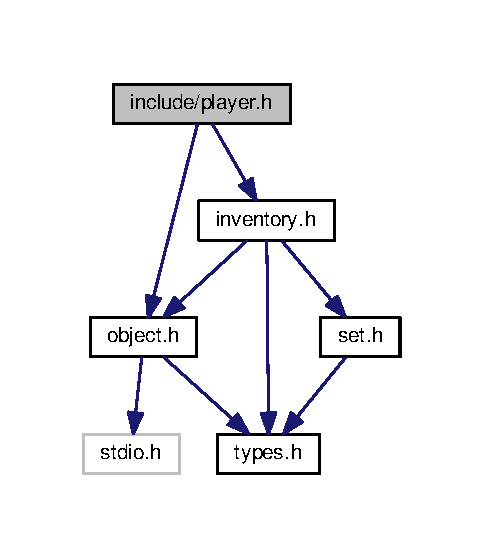
\includegraphics[width=232pt]{player_8h__incl}
\end{center}
\end{figure}
This graph shows which files directly or indirectly include this file\+:
\nopagebreak
\begin{figure}[H]
\begin{center}
\leavevmode
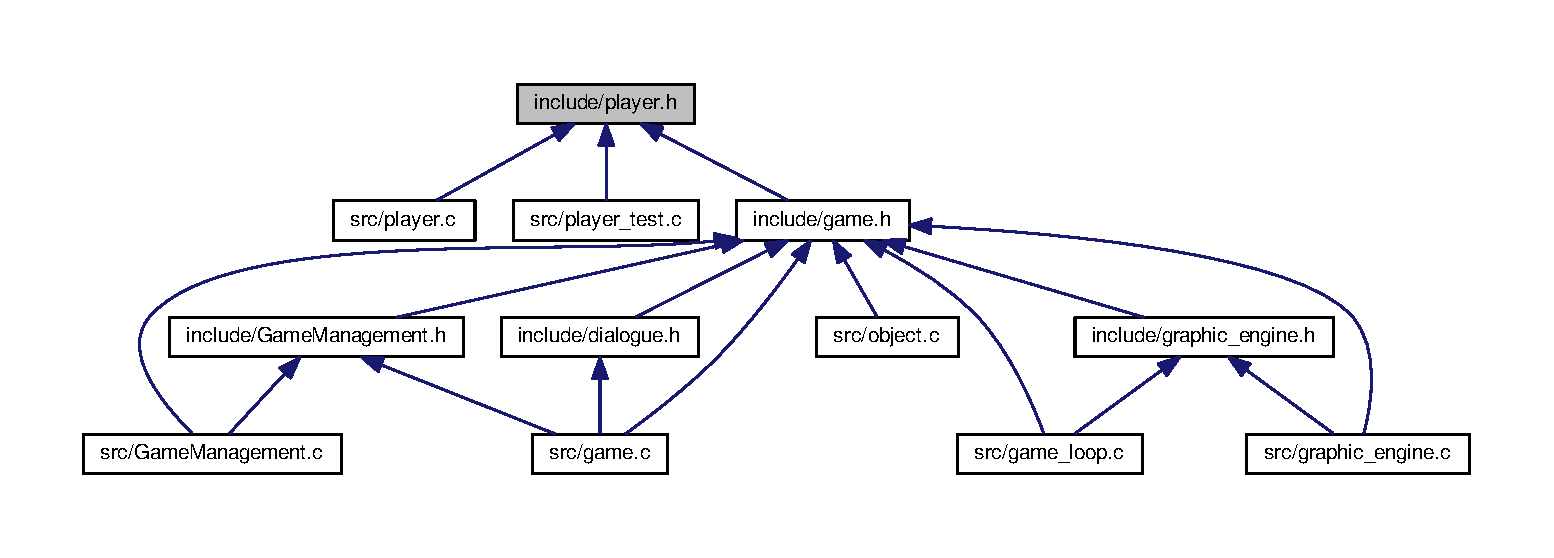
\includegraphics[width=350pt]{player_8h__dep__incl}
\end{center}
\end{figure}
\subsection*{Macros}
\begin{DoxyCompactItemize}
\item 
\#define \hyperlink{player_8h_a5bb4369b60f4886b73026bb884053640}{M\+A\+X\+P\+L\+A\+Y\+N\+A\+ME}~50
\end{DoxyCompactItemize}
\subsection*{Typedefs}
\begin{DoxyCompactItemize}
\item 
typedef struct \hyperlink{struct__Player}{\+\_\+\+Player} \hyperlink{player_8h_af30e2030635a69690f85e48bc6ef202f}{Player}
\begin{DoxyCompactList}\small\item\em player definition \end{DoxyCompactList}\end{DoxyCompactItemize}
\subsection*{Functions}
\begin{DoxyCompactItemize}
\item 
\hyperlink{player_8h_af30e2030635a69690f85e48bc6ef202f}{Player} $\ast$ \hyperlink{player_8h_a97ea1d0deda3c51ef6ce63a13dab7a38}{player\+\_\+create} (\hyperlink{types_8h_a845e604fb28f7e3d97549da3448149d3}{Id} id)
\begin{DoxyCompactList}\small\item\em creates a player \end{DoxyCompactList}\item 
\hyperlink{types_8h_a32c27cc471df37f4fc818d65de0a56c4}{S\+T\+A\+T\+US} \hyperlink{player_8h_a4a602c75f8e3391cbd288c35a83a10fe}{player\+\_\+destroy} (\hyperlink{player_8h_af30e2030635a69690f85e48bc6ef202f}{Player} $\ast$p)
\begin{DoxyCompactList}\small\item\em frees memory \end{DoxyCompactList}\item 
char $\ast$ \hyperlink{player_8h_aaec42336dad00b854be6f071c653d645}{player\+\_\+get\+\_\+name} (\hyperlink{player_8h_af30e2030635a69690f85e48bc6ef202f}{Player} $\ast$p)
\begin{DoxyCompactList}\small\item\em gets the name of a player \end{DoxyCompactList}\item 
\hyperlink{types_8h_a845e604fb28f7e3d97549da3448149d3}{Id} \hyperlink{player_8h_ace9de3676a44420727bcc1d2935ae3e4}{player\+\_\+get\+\_\+id} (\hyperlink{player_8h_af30e2030635a69690f85e48bc6ef202f}{Player} $\ast$p)
\begin{DoxyCompactList}\small\item\em gets the id of a player \end{DoxyCompactList}\item 
\hyperlink{types_8h_a845e604fb28f7e3d97549da3448149d3}{Id} \hyperlink{player_8h_a00fd04dabfe1024ea62fe7c335097db7}{player\+\_\+get\+\_\+location} (\hyperlink{player_8h_af30e2030635a69690f85e48bc6ef202f}{Player} $\ast$p)
\begin{DoxyCompactList}\small\item\em gets the location of an player \end{DoxyCompactList}\item 
\hyperlink{types_8h_a845e604fb28f7e3d97549da3448149d3}{Id} \hyperlink{player_8h_afdb5019868014ca1647d716989664795}{player\+\_\+get\+\_\+object} (\hyperlink{player_8h_af30e2030635a69690f85e48bc6ef202f}{Player} $\ast$p, int position)
\begin{DoxyCompactList}\small\item\em gets an object \end{DoxyCompactList}\item 
\hyperlink{inventory_8h_a2253bf64ac4ce6a9c1d6f39c0b0d32a3}{Inventory} $\ast$ \hyperlink{player_8h_a727c2314037de6f622a513eb1291838f}{player\+\_\+get\+\_\+inventory} (\hyperlink{player_8h_af30e2030635a69690f85e48bc6ef202f}{Player} $\ast$p)
\begin{DoxyCompactList}\small\item\em gets an inventory \end{DoxyCompactList}\item 
\hyperlink{types_8h_a32c27cc471df37f4fc818d65de0a56c4}{S\+T\+A\+T\+US} \hyperlink{player_8h_a5c123d5c69f8d8fa0610c8212e56a3cd}{player\+\_\+set\+\_\+name} (\hyperlink{player_8h_af30e2030635a69690f85e48bc6ef202f}{Player} $\ast$p, char $\ast$name)
\begin{DoxyCompactList}\small\item\em sets name \end{DoxyCompactList}\item 
\hyperlink{types_8h_a32c27cc471df37f4fc818d65de0a56c4}{S\+T\+A\+T\+US} \hyperlink{player_8h_a1df02c30af1e7fd4ed798b62823d0206}{player\+\_\+set\+\_\+id} (\hyperlink{player_8h_af30e2030635a69690f85e48bc6ef202f}{Player} $\ast$p, \hyperlink{types_8h_a845e604fb28f7e3d97549da3448149d3}{Id} id)
\begin{DoxyCompactList}\small\item\em sets an id for a player \end{DoxyCompactList}\item 
\hyperlink{types_8h_a32c27cc471df37f4fc818d65de0a56c4}{S\+T\+A\+T\+US} \hyperlink{player_8h_a53cf87aa437ae42972050bd6da169888}{player\+\_\+set\+\_\+location} (\hyperlink{player_8h_af30e2030635a69690f85e48bc6ef202f}{Player} $\ast$p, \hyperlink{types_8h_a845e604fb28f7e3d97549da3448149d3}{Id} location)
\begin{DoxyCompactList}\small\item\em sets location \end{DoxyCompactList}\item 
\hyperlink{types_8h_a3e5b8192e7d9ffaf3542f1210aec18dd}{B\+O\+OL} \hyperlink{player_8h_a50d2d4bf00b796ffd28bd91bfcfd4685}{player\+\_\+has\+\_\+id} (\hyperlink{player_8h_af30e2030635a69690f85e48bc6ef202f}{Player} $\ast$p, \hyperlink{types_8h_a845e604fb28f7e3d97549da3448149d3}{Id} id)
\begin{DoxyCompactList}\small\item\em checks if player has an id \end{DoxyCompactList}\item 
\hyperlink{types_8h_a32c27cc471df37f4fc818d65de0a56c4}{S\+T\+A\+T\+US} \hyperlink{player_8h_a4096c89077192eedd36aebdba24e9e5e}{player\+\_\+set\+\_\+object} (\hyperlink{player_8h_af30e2030635a69690f85e48bc6ef202f}{Player} $\ast$p, \hyperlink{types_8h_a845e604fb28f7e3d97549da3448149d3}{Id} id)
\begin{DoxyCompactList}\small\item\em sets object \end{DoxyCompactList}\item 
\hyperlink{types_8h_a3e5b8192e7d9ffaf3542f1210aec18dd}{B\+O\+OL} \hyperlink{player_8h_a8b27bf719c2fe3fa9a4712d28dc6f316}{player\+\_\+inventory\+\_\+is\+\_\+empty} (\hyperlink{player_8h_af30e2030635a69690f85e48bc6ef202f}{Player} $\ast$p)
\begin{DoxyCompactList}\small\item\em checks if inventory is empty \end{DoxyCompactList}\item 
\hyperlink{types_8h_a3e5b8192e7d9ffaf3542f1210aec18dd}{B\+O\+OL} \hyperlink{player_8h_a5b4a99b2bcfc728a1bc61d7d33db649e}{player\+\_\+inventory\+\_\+is\+\_\+full} (\hyperlink{player_8h_af30e2030635a69690f85e48bc6ef202f}{Player} $\ast$p)
\begin{DoxyCompactList}\small\item\em checks if inventory is full \end{DoxyCompactList}\item 
\hyperlink{types_8h_a32c27cc471df37f4fc818d65de0a56c4}{S\+T\+A\+T\+US} \hyperlink{player_8h_a45c2b556f12fb90a1b9940bf8d79841f}{player\+\_\+remove\+\_\+object} (\hyperlink{player_8h_af30e2030635a69690f85e48bc6ef202f}{Player} $\ast$p, \hyperlink{types_8h_a845e604fb28f7e3d97549da3448149d3}{Id} id)
\begin{DoxyCompactList}\small\item\em removes an object \end{DoxyCompactList}\end{DoxyCompactItemize}


\subsection{Detailed Description}
Implements the game player commands. 

\begin{DoxyAuthor}{Author}
Borja Pérez 
\end{DoxyAuthor}
\begin{DoxyVersion}{Version}
1.\+6 
\end{DoxyVersion}
\begin{DoxyDate}{Date}
09-\/04-\/2018 
\end{DoxyDate}


\subsection{Macro Definition Documentation}
\index{player.\+h@{player.\+h}!M\+A\+X\+P\+L\+A\+Y\+N\+A\+ME@{M\+A\+X\+P\+L\+A\+Y\+N\+A\+ME}}
\index{M\+A\+X\+P\+L\+A\+Y\+N\+A\+ME@{M\+A\+X\+P\+L\+A\+Y\+N\+A\+ME}!player.\+h@{player.\+h}}
\subsubsection[{\texorpdfstring{M\+A\+X\+P\+L\+A\+Y\+N\+A\+ME}{MAXPLAYNAME}}]{\setlength{\rightskip}{0pt plus 5cm}\#define M\+A\+X\+P\+L\+A\+Y\+N\+A\+ME~50}\hypertarget{player_8h_a5bb4369b60f4886b73026bb884053640}{}\label{player_8h_a5bb4369b60f4886b73026bb884053640}
maximum number of characters for a player name 

\subsection{Typedef Documentation}
\index{player.\+h@{player.\+h}!Player@{Player}}
\index{Player@{Player}!player.\+h@{player.\+h}}
\subsubsection[{\texorpdfstring{Player}{Player}}]{\setlength{\rightskip}{0pt plus 5cm}typedef struct {\bf \+\_\+\+Player} {\bf Player}}\hypertarget{player_8h_af30e2030635a69690f85e48bc6ef202f}{}\label{player_8h_af30e2030635a69690f85e48bc6ef202f}


player definition 

Struct for storing a player and the elements it will use while playing. 

\subsection{Function Documentation}
\index{player.\+h@{player.\+h}!player\+\_\+create@{player\+\_\+create}}
\index{player\+\_\+create@{player\+\_\+create}!player.\+h@{player.\+h}}
\subsubsection[{\texorpdfstring{player\+\_\+create(\+Id id)}{player_create(Id id)}}]{\setlength{\rightskip}{0pt plus 5cm}{\bf Player}$\ast$ player\+\_\+create (
\begin{DoxyParamCaption}
\item[{{\bf Id}}]{id}
\end{DoxyParamCaption}
)}\hypertarget{player_8h_a97ea1d0deda3c51ef6ce63a13dab7a38}{}\label{player_8h_a97ea1d0deda3c51ef6ce63a13dab7a38}


creates a player 

It creates a new object initializing the variables of the structure.

\begin{DoxyAuthor}{Author}
Borja Pérez 
\end{DoxyAuthor}

\begin{DoxyParams}{Parameters}
{\em id} & long int. \\
\hline
\end{DoxyParams}
\begin{DoxyReturn}{Returns}
pointer to player, N\+U\+LL if something goes wrong. 
\end{DoxyReturn}
\index{player.\+h@{player.\+h}!player\+\_\+destroy@{player\+\_\+destroy}}
\index{player\+\_\+destroy@{player\+\_\+destroy}!player.\+h@{player.\+h}}
\subsubsection[{\texorpdfstring{player\+\_\+destroy(\+Player $\ast$p)}{player_destroy(Player *p)}}]{\setlength{\rightskip}{0pt plus 5cm}{\bf S\+T\+A\+T\+US} player\+\_\+destroy (
\begin{DoxyParamCaption}
\item[{{\bf Player} $\ast$}]{p}
\end{DoxyParamCaption}
)}\hypertarget{player_8h_a4a602c75f8e3391cbd288c35a83a10fe}{}\label{player_8h_a4a602c75f8e3391cbd288c35a83a10fe}


frees memory 

Receives pointer to player and frees the memory it occupied.

\begin{DoxyAuthor}{Author}
Borja Pérez 
\end{DoxyAuthor}

\begin{DoxyParams}{Parameters}
{\em p} & pointer to player. \\
\hline
\end{DoxyParams}
\begin{DoxyReturn}{Returns}
S\+T\+A\+T\+US, E\+R\+R\+OR if argument received is N\+U\+LL, if not, OK. 
\end{DoxyReturn}
\index{player.\+h@{player.\+h}!player\+\_\+get\+\_\+id@{player\+\_\+get\+\_\+id}}
\index{player\+\_\+get\+\_\+id@{player\+\_\+get\+\_\+id}!player.\+h@{player.\+h}}
\subsubsection[{\texorpdfstring{player\+\_\+get\+\_\+id(\+Player $\ast$p)}{player_get_id(Player *p)}}]{\setlength{\rightskip}{0pt plus 5cm}{\bf Id} player\+\_\+get\+\_\+id (
\begin{DoxyParamCaption}
\item[{{\bf Player} $\ast$}]{p}
\end{DoxyParamCaption}
)}\hypertarget{player_8h_ace9de3676a44420727bcc1d2935ae3e4}{}\label{player_8h_ace9de3676a44420727bcc1d2935ae3e4}


gets the id of a player 

Function in charge of getting the id of an player by using a pointer to it.

\begin{DoxyAuthor}{Author}
Borja Pérez 
\end{DoxyAuthor}

\begin{DoxyParams}{Parameters}
{\em p} & pointer to player. \\
\hline
\end{DoxyParams}
\begin{DoxyReturn}{Returns}
Id, N\+O\+\_\+\+ID if object is pointing N\+U\+LL. 
\end{DoxyReturn}
\index{player.\+h@{player.\+h}!player\+\_\+get\+\_\+inventory@{player\+\_\+get\+\_\+inventory}}
\index{player\+\_\+get\+\_\+inventory@{player\+\_\+get\+\_\+inventory}!player.\+h@{player.\+h}}
\subsubsection[{\texorpdfstring{player\+\_\+get\+\_\+inventory(\+Player $\ast$p)}{player_get_inventory(Player *p)}}]{\setlength{\rightskip}{0pt plus 5cm}{\bf Inventory}$\ast$ player\+\_\+get\+\_\+inventory (
\begin{DoxyParamCaption}
\item[{{\bf Player} $\ast$}]{p}
\end{DoxyParamCaption}
)}\hypertarget{player_8h_a727c2314037de6f622a513eb1291838f}{}\label{player_8h_a727c2314037de6f622a513eb1291838f}


gets an inventory 

The player has an inventory that enables the player to take more than one object.

\begin{DoxyAuthor}{Author}
Borja Pérez 
\end{DoxyAuthor}

\begin{DoxyParams}{Parameters}
{\em p} & pointer to player. \\
\hline
\end{DoxyParams}
\begin{DoxyReturn}{Returns}
pointer to inventory (objects). 
\end{DoxyReturn}
\index{player.\+h@{player.\+h}!player\+\_\+get\+\_\+location@{player\+\_\+get\+\_\+location}}
\index{player\+\_\+get\+\_\+location@{player\+\_\+get\+\_\+location}!player.\+h@{player.\+h}}
\subsubsection[{\texorpdfstring{player\+\_\+get\+\_\+location(\+Player $\ast$p)}{player_get_location(Player *p)}}]{\setlength{\rightskip}{0pt plus 5cm}{\bf Id} player\+\_\+get\+\_\+location (
\begin{DoxyParamCaption}
\item[{{\bf Player} $\ast$}]{p}
\end{DoxyParamCaption}
)}\hypertarget{player_8h_a00fd04dabfe1024ea62fe7c335097db7}{}\label{player_8h_a00fd04dabfe1024ea62fe7c335097db7}


gets the location of an player 

Function in charge of getting the location of a player and returning it.

\begin{DoxyAuthor}{Author}
Borja Pérez 
\end{DoxyAuthor}

\begin{DoxyParams}{Parameters}
{\em p} & pointer to player \\
\hline
\end{DoxyParams}
\begin{DoxyReturn}{Returns}
Id, N\+O\+\_\+\+ID if inventory is pointing N\+U\+LL. 
\end{DoxyReturn}
\index{player.\+h@{player.\+h}!player\+\_\+get\+\_\+name@{player\+\_\+get\+\_\+name}}
\index{player\+\_\+get\+\_\+name@{player\+\_\+get\+\_\+name}!player.\+h@{player.\+h}}
\subsubsection[{\texorpdfstring{player\+\_\+get\+\_\+name(\+Player $\ast$p)}{player_get_name(Player *p)}}]{\setlength{\rightskip}{0pt plus 5cm}char$\ast$ player\+\_\+get\+\_\+name (
\begin{DoxyParamCaption}
\item[{{\bf Player} $\ast$}]{p}
\end{DoxyParamCaption}
)}\hypertarget{player_8h_aaec42336dad00b854be6f071c653d645}{}\label{player_8h_aaec42336dad00b854be6f071c653d645}


gets the name of a player 

Function in charge of showing the name of a player that has already been set.

\begin{DoxyAuthor}{Author}
Borja Pérez 
\end{DoxyAuthor}

\begin{DoxyParams}{Parameters}
{\em p} & pointer to object. \\
\hline
\end{DoxyParams}
\begin{DoxyReturn}{Returns}
char (name of the player). 
\end{DoxyReturn}
\index{player.\+h@{player.\+h}!player\+\_\+get\+\_\+object@{player\+\_\+get\+\_\+object}}
\index{player\+\_\+get\+\_\+object@{player\+\_\+get\+\_\+object}!player.\+h@{player.\+h}}
\subsubsection[{\texorpdfstring{player\+\_\+get\+\_\+object(\+Player $\ast$p, int position)}{player_get_object(Player *p, int position)}}]{\setlength{\rightskip}{0pt plus 5cm}{\bf Id} player\+\_\+get\+\_\+object (
\begin{DoxyParamCaption}
\item[{{\bf Player} $\ast$}]{p, }
\item[{int}]{position}
\end{DoxyParamCaption}
)}\hypertarget{player_8h_afdb5019868014ca1647d716989664795}{}\label{player_8h_afdb5019868014ca1647d716989664795}


gets an object 

Function in charge of getting the object that the player will carry.

\begin{DoxyAuthor}{Author}
Borja Pérez 
\end{DoxyAuthor}

\begin{DoxyParams}{Parameters}
{\em p} & pointer to player. \\
\hline
{\em position} & int (position of the object). \\
\hline
\end{DoxyParams}
\begin{DoxyReturn}{Returns}
Id, N\+O\+\_\+\+ID if inventory is pointing N\+U\+LL. 
\end{DoxyReturn}
\index{player.\+h@{player.\+h}!player\+\_\+has\+\_\+id@{player\+\_\+has\+\_\+id}}
\index{player\+\_\+has\+\_\+id@{player\+\_\+has\+\_\+id}!player.\+h@{player.\+h}}
\subsubsection[{\texorpdfstring{player\+\_\+has\+\_\+id(\+Player $\ast$p, Id id)}{player_has_id(Player *p, Id id)}}]{\setlength{\rightskip}{0pt plus 5cm}{\bf B\+O\+OL} player\+\_\+has\+\_\+id (
\begin{DoxyParamCaption}
\item[{{\bf Player} $\ast$}]{p, }
\item[{{\bf Id}}]{id}
\end{DoxyParamCaption}
)}\hypertarget{player_8h_a50d2d4bf00b796ffd28bd91bfcfd4685}{}\label{player_8h_a50d2d4bf00b796ffd28bd91bfcfd4685}


checks if player has an id 

Function in charge of making sure that the player is getting an id.

\begin{DoxyAuthor}{Author}
Borja Pérez 
\end{DoxyAuthor}

\begin{DoxyParams}{Parameters}
{\em p} & pointer to player. \\
\hline
{\em id} & long int. \\
\hline
\end{DoxyParams}
\begin{DoxyReturn}{Returns}
B\+O\+OL, F\+A\+L\+SE if when checking is not correct, if it is correct, T\+R\+UE. 
\end{DoxyReturn}
\index{player.\+h@{player.\+h}!player\+\_\+inventory\+\_\+is\+\_\+empty@{player\+\_\+inventory\+\_\+is\+\_\+empty}}
\index{player\+\_\+inventory\+\_\+is\+\_\+empty@{player\+\_\+inventory\+\_\+is\+\_\+empty}!player.\+h@{player.\+h}}
\subsubsection[{\texorpdfstring{player\+\_\+inventory\+\_\+is\+\_\+empty(\+Player $\ast$p)}{player_inventory_is_empty(Player *p)}}]{\setlength{\rightskip}{0pt plus 5cm}{\bf B\+O\+OL} player\+\_\+inventory\+\_\+is\+\_\+empty (
\begin{DoxyParamCaption}
\item[{{\bf Player} $\ast$}]{p}
\end{DoxyParamCaption}
)}\hypertarget{player_8h_a8b27bf719c2fe3fa9a4712d28dc6f316}{}\label{player_8h_a8b27bf719c2fe3fa9a4712d28dc6f316}


checks if inventory is empty 

Function in charge of making sure that the inventory is empty using a pointer to player in order to work with other modules more easily.

\begin{DoxyAuthor}{Author}
Borja Pérez 
\end{DoxyAuthor}

\begin{DoxyParams}{Parameters}
{\em p} & pointer to player. \\
\hline
\end{DoxyParams}
\begin{DoxyReturn}{Returns}
B\+O\+OL, F\+A\+L\+SE if when checking is not correct, if it is correct, T\+R\+UE. 
\end{DoxyReturn}
\index{player.\+h@{player.\+h}!player\+\_\+inventory\+\_\+is\+\_\+full@{player\+\_\+inventory\+\_\+is\+\_\+full}}
\index{player\+\_\+inventory\+\_\+is\+\_\+full@{player\+\_\+inventory\+\_\+is\+\_\+full}!player.\+h@{player.\+h}}
\subsubsection[{\texorpdfstring{player\+\_\+inventory\+\_\+is\+\_\+full(\+Player $\ast$p)}{player_inventory_is_full(Player *p)}}]{\setlength{\rightskip}{0pt plus 5cm}{\bf B\+O\+OL} player\+\_\+inventory\+\_\+is\+\_\+full (
\begin{DoxyParamCaption}
\item[{{\bf Player} $\ast$}]{p}
\end{DoxyParamCaption}
)}\hypertarget{player_8h_a5b4a99b2bcfc728a1bc61d7d33db649e}{}\label{player_8h_a5b4a99b2bcfc728a1bc61d7d33db649e}


checks if inventory is full 

Function in charge of making sure that the inventory is full using a pointer to player in order to work with other modules more easily.

\begin{DoxyAuthor}{Author}
Borja Pérez 
\end{DoxyAuthor}

\begin{DoxyParams}{Parameters}
{\em p} & pointer to player. \\
\hline
\end{DoxyParams}
\begin{DoxyReturn}{Returns}
B\+O\+OL, F\+A\+L\+SE if when checking is not correct, if it is correct, T\+R\+UE. 
\end{DoxyReturn}
\index{player.\+h@{player.\+h}!player\+\_\+remove\+\_\+object@{player\+\_\+remove\+\_\+object}}
\index{player\+\_\+remove\+\_\+object@{player\+\_\+remove\+\_\+object}!player.\+h@{player.\+h}}
\subsubsection[{\texorpdfstring{player\+\_\+remove\+\_\+object(\+Player $\ast$p, Id id)}{player_remove_object(Player *p, Id id)}}]{\setlength{\rightskip}{0pt plus 5cm}{\bf S\+T\+A\+T\+US} player\+\_\+remove\+\_\+object (
\begin{DoxyParamCaption}
\item[{{\bf Player} $\ast$}]{p, }
\item[{{\bf Id}}]{id}
\end{DoxyParamCaption}
)}\hypertarget{player_8h_a45c2b556f12fb90a1b9940bf8d79841f}{}\label{player_8h_a45c2b556f12fb90a1b9940bf8d79841f}


removes an object 

Deletes an object by using other functions prepared for this specific one.

\begin{DoxyAuthor}{Author}
Borja Pérez 
\end{DoxyAuthor}

\begin{DoxyParams}{Parameters}
{\em p} & pointer to player. \\
\hline
{\em id} & long int. \\
\hline
\end{DoxyParams}
\begin{DoxyReturn}{Returns}
S\+T\+A\+T\+US, E\+R\+R\+OR if argument received is N\+U\+LL, if not, OK. 
\end{DoxyReturn}
\index{player.\+h@{player.\+h}!player\+\_\+set\+\_\+id@{player\+\_\+set\+\_\+id}}
\index{player\+\_\+set\+\_\+id@{player\+\_\+set\+\_\+id}!player.\+h@{player.\+h}}
\subsubsection[{\texorpdfstring{player\+\_\+set\+\_\+id(\+Player $\ast$p, Id id)}{player_set_id(Player *p, Id id)}}]{\setlength{\rightskip}{0pt plus 5cm}{\bf S\+T\+A\+T\+US} player\+\_\+set\+\_\+id (
\begin{DoxyParamCaption}
\item[{{\bf Player} $\ast$}]{p, }
\item[{{\bf Id}}]{id}
\end{DoxyParamCaption}
)}\hypertarget{player_8h_a1df02c30af1e7fd4ed798b62823d0206}{}\label{player_8h_a1df02c30af1e7fd4ed798b62823d0206}


sets an id for a player 

Function in charge of changing a player\textquotesingle{}s id.

\begin{DoxyAuthor}{Author}
Borja Pérez 
\end{DoxyAuthor}

\begin{DoxyParams}{Parameters}
{\em p} & pointer to player. \\
\hline
{\em id} & long int. \\
\hline
\end{DoxyParams}
\begin{DoxyReturn}{Returns}
S\+T\+A\+T\+US, E\+R\+R\+OR if argument received is N\+U\+LL, if not, OK. 
\end{DoxyReturn}
\index{player.\+h@{player.\+h}!player\+\_\+set\+\_\+location@{player\+\_\+set\+\_\+location}}
\index{player\+\_\+set\+\_\+location@{player\+\_\+set\+\_\+location}!player.\+h@{player.\+h}}
\subsubsection[{\texorpdfstring{player\+\_\+set\+\_\+location(\+Player $\ast$p, Id location)}{player_set_location(Player *p, Id location)}}]{\setlength{\rightskip}{0pt plus 5cm}{\bf S\+T\+A\+T\+US} player\+\_\+set\+\_\+location (
\begin{DoxyParamCaption}
\item[{{\bf Player} $\ast$}]{p, }
\item[{{\bf Id}}]{location}
\end{DoxyParamCaption}
)}\hypertarget{player_8h_a53cf87aa437ae42972050bd6da169888}{}\label{player_8h_a53cf87aa437ae42972050bd6da169888}


sets location 

Changes a player\textquotesingle{}s location.

\begin{DoxyAuthor}{Author}
Borja Pérez 
\end{DoxyAuthor}

\begin{DoxyParams}{Parameters}
{\em p} & pointer to player. \\
\hline
{\em location} & The id of the player\textquotesingle{}s location. \\
\hline
\end{DoxyParams}
\begin{DoxyReturn}{Returns}
S\+T\+A\+T\+US, E\+R\+R\+OR if argument received is N\+U\+LL, if not, OK. 
\end{DoxyReturn}
\index{player.\+h@{player.\+h}!player\+\_\+set\+\_\+name@{player\+\_\+set\+\_\+name}}
\index{player\+\_\+set\+\_\+name@{player\+\_\+set\+\_\+name}!player.\+h@{player.\+h}}
\subsubsection[{\texorpdfstring{player\+\_\+set\+\_\+name(\+Player $\ast$p, char $\ast$name)}{player_set_name(Player *p, char *name)}}]{\setlength{\rightskip}{0pt plus 5cm}{\bf S\+T\+A\+T\+US} player\+\_\+set\+\_\+name (
\begin{DoxyParamCaption}
\item[{{\bf Player} $\ast$}]{p, }
\item[{char $\ast$}]{name}
\end{DoxyParamCaption}
)}\hypertarget{player_8h_a5c123d5c69f8d8fa0610c8212e56a3cd}{}\label{player_8h_a5c123d5c69f8d8fa0610c8212e56a3cd}


sets name 

Function in charge of changing the name of a player.

\begin{DoxyAuthor}{Author}
Borja Pérez 
\end{DoxyAuthor}

\begin{DoxyParams}{Parameters}
{\em p} & pointer to player. \\
\hline
{\em name} & char( string for the name of the player). \\
\hline
\end{DoxyParams}
\begin{DoxyReturn}{Returns}
S\+T\+A\+T\+US, E\+R\+R\+OR if argument received is N\+U\+LL, if not, OK. 
\end{DoxyReturn}
\index{player.\+h@{player.\+h}!player\+\_\+set\+\_\+object@{player\+\_\+set\+\_\+object}}
\index{player\+\_\+set\+\_\+object@{player\+\_\+set\+\_\+object}!player.\+h@{player.\+h}}
\subsubsection[{\texorpdfstring{player\+\_\+set\+\_\+object(\+Player $\ast$p, Id id)}{player_set_object(Player *p, Id id)}}]{\setlength{\rightskip}{0pt plus 5cm}{\bf S\+T\+A\+T\+US} player\+\_\+set\+\_\+object (
\begin{DoxyParamCaption}
\item[{{\bf Player} $\ast$}]{p, }
\item[{{\bf Id}}]{id}
\end{DoxyParamCaption}
)}\hypertarget{player_8h_a4096c89077192eedd36aebdba24e9e5e}{}\label{player_8h_a4096c89077192eedd36aebdba24e9e5e}


sets object 

Changes the object carried by a player.

\begin{DoxyAuthor}{Author}
Borja Pérez 
\end{DoxyAuthor}

\begin{DoxyParams}{Parameters}
{\em p} & pointer to player. \\
\hline
{\em id} & long int. \\
\hline
\end{DoxyParams}
\begin{DoxyReturn}{Returns}
S\+T\+A\+T\+US, E\+R\+R\+OR if argument received is N\+U\+LL, if not, OK. 
\end{DoxyReturn}

\hypertarget{player__test_8h}{}\section{include/player\+\_\+test.h File Reference}
\label{player__test_8h}\index{include/player\+\_\+test.\+h@{include/player\+\_\+test.\+h}}


It declares the tests for the player module.  


{\ttfamily \#include $<$stdio.\+h$>$}\\*
{\ttfamily \#include \char`\"{}types.\+h\char`\"{}}\\*
Include dependency graph for player\+\_\+test.\+h\+:
\nopagebreak
\begin{figure}[H]
\begin{center}
\leavevmode
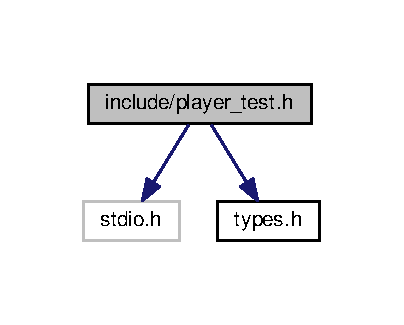
\includegraphics[width=194pt]{player__test_8h__incl}
\end{center}
\end{figure}
This graph shows which files directly or indirectly include this file\+:
\nopagebreak
\begin{figure}[H]
\begin{center}
\leavevmode
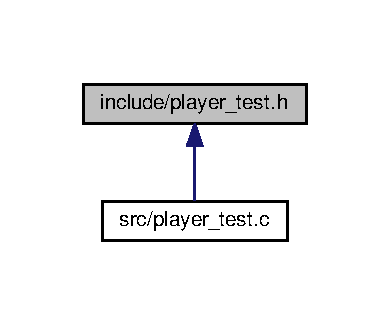
\includegraphics[width=187pt]{player__test_8h__dep__incl}
\end{center}
\end{figure}
\subsection*{Functions}
\begin{DoxyCompactItemize}
\item 
void \hyperlink{player__test_8h_ab29768452373e16bb6aaa1f7998f62fb}{test1\+\_\+player\+\_\+create} ()
\item 
void \hyperlink{player__test_8h_a4f6eca5f9d8c08d2a7fc70c209ecf854}{test2\+\_\+player\+\_\+create} ()
\item 
void \hyperlink{player__test_8h_aae84b37f9cc0fbde18a62807385c359a}{test3\+\_\+player\+\_\+create} ()
\item 
void \hyperlink{player__test_8h_a14d75d99f9fce3bd703b0c242c8690f9}{test1\+\_\+player\+\_\+destroy} ()
\item 
void \hyperlink{player__test_8h_ae873be01647faf96d3906aa9629e87f0}{test2\+\_\+player\+\_\+destroy} ()
\item 
void \hyperlink{player__test_8h_a8841b3b289649eb76edaa8110ad5899c}{test1\+\_\+player\+\_\+has\+\_\+id} ()
\item 
void \hyperlink{player__test_8h_afa75f333281fc35b24968a5629f09b0b}{test2\+\_\+player\+\_\+has\+\_\+id} ()
\item 
void \hyperlink{player__test_8h_a3b450c7540eddb05810dc9c25e4de082}{test3\+\_\+player\+\_\+has\+\_\+id} ()
\item 
void \hyperlink{player__test_8h_ad4a86b57bc18593265c205d7b27b9ecb}{test1\+\_\+player\+\_\+get\+\_\+inventory} ()
\item 
void \hyperlink{player__test_8h_a8f3a62c708fbed848568841ca8b1cd26}{test2\+\_\+player\+\_\+get\+\_\+inventory} ()
\item 
void \hyperlink{player__test_8h_a53eb6ee101f01fe988c5da03129d2e2f}{test1\+\_\+player\+\_\+get\+\_\+object} ()
\item 
void \hyperlink{player__test_8h_a83e8fea42cd87151cd67d0643a78134f}{test2\+\_\+player\+\_\+get\+\_\+object} ()
\item 
void \hyperlink{player__test_8h_ac8d8b030a98c0e44f4e98e08cda59537}{test1\+\_\+player\+\_\+set\+\_\+object} ()
\item 
void \hyperlink{player__test_8h_a9e7db6b857907187146df64abd16aca5}{test2\+\_\+player\+\_\+set\+\_\+object} ()
\item 
void \hyperlink{player__test_8h_a0685839b423f685dcdabb7b9fe411cd1}{test1\+\_\+player\+\_\+remove\+\_\+object} ()
\item 
void \hyperlink{player__test_8h_af9e74e12ad6961761f1ff61afa56be3e}{test2\+\_\+player\+\_\+remove\+\_\+object} ()
\end{DoxyCompactItemize}


\subsection{Detailed Description}
It declares the tests for the player module. 

\begin{DoxyAuthor}{Author}
Andrés Mena 
\end{DoxyAuthor}
\begin{DoxyVersion}{Version}
2.\+0 
\end{DoxyVersion}
\begin{DoxyDate}{Date}
01-\/04-\/2018 
\end{DoxyDate}
\begin{DoxyCopyright}{Copyright}
G\+NU Public License 
\end{DoxyCopyright}


\subsection{Function Documentation}
\index{player\+\_\+test.\+h@{player\+\_\+test.\+h}!test1\+\_\+player\+\_\+create@{test1\+\_\+player\+\_\+create}}
\index{test1\+\_\+player\+\_\+create@{test1\+\_\+player\+\_\+create}!player\+\_\+test.\+h@{player\+\_\+test.\+h}}
\subsubsection[{\texorpdfstring{test1\+\_\+player\+\_\+create()}{test1_player_create()}}]{\setlength{\rightskip}{0pt plus 5cm}void test1\+\_\+player\+\_\+create (
\begin{DoxyParamCaption}
{}
\end{DoxyParamCaption}
)}\hypertarget{player__test_8h_ab29768452373e16bb6aaa1f7998f62fb}{}\label{player__test_8h_ab29768452373e16bb6aaa1f7998f62fb}
\begin{DoxyRefDesc}{Test}
\item[\hyperlink{test__test000105}{Test}]Test player creation \end{DoxyRefDesc}
\begin{DoxyPrecond}{Precondition}
ID 
\end{DoxyPrecond}
\begin{DoxyPostcond}{Postcondition}
Non N\+U\+LL pointer to player 
\end{DoxyPostcond}
\index{player\+\_\+test.\+h@{player\+\_\+test.\+h}!test1\+\_\+player\+\_\+destroy@{test1\+\_\+player\+\_\+destroy}}
\index{test1\+\_\+player\+\_\+destroy@{test1\+\_\+player\+\_\+destroy}!player\+\_\+test.\+h@{player\+\_\+test.\+h}}
\subsubsection[{\texorpdfstring{test1\+\_\+player\+\_\+destroy()}{test1_player_destroy()}}]{\setlength{\rightskip}{0pt plus 5cm}void test1\+\_\+player\+\_\+destroy (
\begin{DoxyParamCaption}
{}
\end{DoxyParamCaption}
)}\hypertarget{player__test_8h_a14d75d99f9fce3bd703b0c242c8690f9}{}\label{player__test_8h_a14d75d99f9fce3bd703b0c242c8690f9}
\begin{DoxyRefDesc}{Test}
\item[\hyperlink{test__test000108}{Test}]Test player creation \end{DoxyRefDesc}
\begin{DoxyPrecond}{Precondition}
N\+U\+LL pointer to player 
\end{DoxyPrecond}
\begin{DoxyPostcond}{Postcondition}
S\+T\+A\+T\+US == E\+R\+R\+OR 
\end{DoxyPostcond}
\index{player\+\_\+test.\+h@{player\+\_\+test.\+h}!test1\+\_\+player\+\_\+get\+\_\+inventory@{test1\+\_\+player\+\_\+get\+\_\+inventory}}
\index{test1\+\_\+player\+\_\+get\+\_\+inventory@{test1\+\_\+player\+\_\+get\+\_\+inventory}!player\+\_\+test.\+h@{player\+\_\+test.\+h}}
\subsubsection[{\texorpdfstring{test1\+\_\+player\+\_\+get\+\_\+inventory()}{test1_player_get_inventory()}}]{\setlength{\rightskip}{0pt plus 5cm}void test1\+\_\+player\+\_\+get\+\_\+inventory (
\begin{DoxyParamCaption}
{}
\end{DoxyParamCaption}
)}\hypertarget{player__test_8h_ad4a86b57bc18593265c205d7b27b9ecb}{}\label{player__test_8h_ad4a86b57bc18593265c205d7b27b9ecb}
\begin{DoxyRefDesc}{Test}
\item[\hyperlink{test__test000113}{Test}]Test player inventory \end{DoxyRefDesc}
\begin{DoxyPrecond}{Precondition}
N\+U\+LL pointer to player 
\end{DoxyPrecond}
\begin{DoxyPostcond}{Postcondition}
N\+U\+LL 
\end{DoxyPostcond}
\index{player\+\_\+test.\+h@{player\+\_\+test.\+h}!test1\+\_\+player\+\_\+get\+\_\+object@{test1\+\_\+player\+\_\+get\+\_\+object}}
\index{test1\+\_\+player\+\_\+get\+\_\+object@{test1\+\_\+player\+\_\+get\+\_\+object}!player\+\_\+test.\+h@{player\+\_\+test.\+h}}
\subsubsection[{\texorpdfstring{test1\+\_\+player\+\_\+get\+\_\+object()}{test1_player_get_object()}}]{\setlength{\rightskip}{0pt plus 5cm}void test1\+\_\+player\+\_\+get\+\_\+object (
\begin{DoxyParamCaption}
{}
\end{DoxyParamCaption}
)}\hypertarget{player__test_8h_a53eb6ee101f01fe988c5da03129d2e2f}{}\label{player__test_8h_a53eb6ee101f01fe988c5da03129d2e2f}
\begin{DoxyRefDesc}{Test}
\item[\hyperlink{test__test000115}{Test}]Test getting objects from player \end{DoxyRefDesc}
\begin{DoxyPrecond}{Precondition}
N\+U\+LL pointer to player 
\end{DoxyPrecond}
\begin{DoxyPostcond}{Postcondition}
N\+O\+\_\+\+ID 
\end{DoxyPostcond}
\index{player\+\_\+test.\+h@{player\+\_\+test.\+h}!test1\+\_\+player\+\_\+has\+\_\+id@{test1\+\_\+player\+\_\+has\+\_\+id}}
\index{test1\+\_\+player\+\_\+has\+\_\+id@{test1\+\_\+player\+\_\+has\+\_\+id}!player\+\_\+test.\+h@{player\+\_\+test.\+h}}
\subsubsection[{\texorpdfstring{test1\+\_\+player\+\_\+has\+\_\+id()}{test1_player_has_id()}}]{\setlength{\rightskip}{0pt plus 5cm}void test1\+\_\+player\+\_\+has\+\_\+id (
\begin{DoxyParamCaption}
{}
\end{DoxyParamCaption}
)}\hypertarget{player__test_8h_a8841b3b289649eb76edaa8110ad5899c}{}\label{player__test_8h_a8841b3b289649eb76edaa8110ad5899c}
\begin{DoxyRefDesc}{Test}
\item[\hyperlink{test__test000110}{Test}]Test if player has id \end{DoxyRefDesc}
\begin{DoxyPrecond}{Precondition}
N\+U\+LL pointer to player 
\end{DoxyPrecond}
\begin{DoxyPostcond}{Postcondition}
B\+O\+OL == F\+A\+L\+SE 
\end{DoxyPostcond}
\index{player\+\_\+test.\+h@{player\+\_\+test.\+h}!test1\+\_\+player\+\_\+remove\+\_\+object@{test1\+\_\+player\+\_\+remove\+\_\+object}}
\index{test1\+\_\+player\+\_\+remove\+\_\+object@{test1\+\_\+player\+\_\+remove\+\_\+object}!player\+\_\+test.\+h@{player\+\_\+test.\+h}}
\subsubsection[{\texorpdfstring{test1\+\_\+player\+\_\+remove\+\_\+object()}{test1_player_remove_object()}}]{\setlength{\rightskip}{0pt plus 5cm}void test1\+\_\+player\+\_\+remove\+\_\+object (
\begin{DoxyParamCaption}
{}
\end{DoxyParamCaption}
)}\hypertarget{player__test_8h_a0685839b423f685dcdabb7b9fe411cd1}{}\label{player__test_8h_a0685839b423f685dcdabb7b9fe411cd1}
\begin{DoxyRefDesc}{Test}
\item[\hyperlink{test__test000119}{Test}]Test removing objects from player \end{DoxyRefDesc}
\begin{DoxyPrecond}{Precondition}
N\+U\+LL pointer to player 
\end{DoxyPrecond}
\begin{DoxyPostcond}{Postcondition}
E\+R\+R\+OR 
\end{DoxyPostcond}
\index{player\+\_\+test.\+h@{player\+\_\+test.\+h}!test1\+\_\+player\+\_\+set\+\_\+object@{test1\+\_\+player\+\_\+set\+\_\+object}}
\index{test1\+\_\+player\+\_\+set\+\_\+object@{test1\+\_\+player\+\_\+set\+\_\+object}!player\+\_\+test.\+h@{player\+\_\+test.\+h}}
\subsubsection[{\texorpdfstring{test1\+\_\+player\+\_\+set\+\_\+object()}{test1_player_set_object()}}]{\setlength{\rightskip}{0pt plus 5cm}void test1\+\_\+player\+\_\+set\+\_\+object (
\begin{DoxyParamCaption}
{}
\end{DoxyParamCaption}
)}\hypertarget{player__test_8h_ac8d8b030a98c0e44f4e98e08cda59537}{}\label{player__test_8h_ac8d8b030a98c0e44f4e98e08cda59537}
\begin{DoxyRefDesc}{Test}
\item[\hyperlink{test__test000117}{Test}]Test setting objects to player \end{DoxyRefDesc}
\begin{DoxyPrecond}{Precondition}
N\+U\+LL pointer to player 
\end{DoxyPrecond}
\begin{DoxyPostcond}{Postcondition}
E\+R\+R\+OR 
\end{DoxyPostcond}
\index{player\+\_\+test.\+h@{player\+\_\+test.\+h}!test2\+\_\+player\+\_\+create@{test2\+\_\+player\+\_\+create}}
\index{test2\+\_\+player\+\_\+create@{test2\+\_\+player\+\_\+create}!player\+\_\+test.\+h@{player\+\_\+test.\+h}}
\subsubsection[{\texorpdfstring{test2\+\_\+player\+\_\+create()}{test2_player_create()}}]{\setlength{\rightskip}{0pt plus 5cm}void test2\+\_\+player\+\_\+create (
\begin{DoxyParamCaption}
{}
\end{DoxyParamCaption}
)}\hypertarget{player__test_8h_a4f6eca5f9d8c08d2a7fc70c209ecf854}{}\label{player__test_8h_a4f6eca5f9d8c08d2a7fc70c209ecf854}
\begin{DoxyRefDesc}{Test}
\item[\hyperlink{test__test000106}{Test}]Test player creation \end{DoxyRefDesc}
\begin{DoxyPrecond}{Precondition}
Player ID 
\end{DoxyPrecond}
\begin{DoxyPostcond}{Postcondition}
Player\+\_\+\+ID == Supplied player Id 
\end{DoxyPostcond}
\index{player\+\_\+test.\+h@{player\+\_\+test.\+h}!test2\+\_\+player\+\_\+destroy@{test2\+\_\+player\+\_\+destroy}}
\index{test2\+\_\+player\+\_\+destroy@{test2\+\_\+player\+\_\+destroy}!player\+\_\+test.\+h@{player\+\_\+test.\+h}}
\subsubsection[{\texorpdfstring{test2\+\_\+player\+\_\+destroy()}{test2_player_destroy()}}]{\setlength{\rightskip}{0pt plus 5cm}void test2\+\_\+player\+\_\+destroy (
\begin{DoxyParamCaption}
{}
\end{DoxyParamCaption}
)}\hypertarget{player__test_8h_ae873be01647faf96d3906aa9629e87f0}{}\label{player__test_8h_ae873be01647faf96d3906aa9629e87f0}
\begin{DoxyRefDesc}{Test}
\item[\hyperlink{test__test000109}{Test}]Test player creation \end{DoxyRefDesc}
\begin{DoxyPrecond}{Precondition}
Pointer to player 
\end{DoxyPrecond}
\begin{DoxyPostcond}{Postcondition}
S\+T\+A\+T\+US == OK 
\end{DoxyPostcond}
\index{player\+\_\+test.\+h@{player\+\_\+test.\+h}!test2\+\_\+player\+\_\+get\+\_\+inventory@{test2\+\_\+player\+\_\+get\+\_\+inventory}}
\index{test2\+\_\+player\+\_\+get\+\_\+inventory@{test2\+\_\+player\+\_\+get\+\_\+inventory}!player\+\_\+test.\+h@{player\+\_\+test.\+h}}
\subsubsection[{\texorpdfstring{test2\+\_\+player\+\_\+get\+\_\+inventory()}{test2_player_get_inventory()}}]{\setlength{\rightskip}{0pt plus 5cm}void test2\+\_\+player\+\_\+get\+\_\+inventory (
\begin{DoxyParamCaption}
{}
\end{DoxyParamCaption}
)}\hypertarget{player__test_8h_a8f3a62c708fbed848568841ca8b1cd26}{}\label{player__test_8h_a8f3a62c708fbed848568841ca8b1cd26}
\begin{DoxyRefDesc}{Test}
\item[\hyperlink{test__test000114}{Test}]Test player inventory \end{DoxyRefDesc}
\begin{DoxyPrecond}{Precondition}
Pointer to player and inventory 
\end{DoxyPrecond}
\begin{DoxyPostcond}{Postcondition}
inventory not N\+U\+LL 
\end{DoxyPostcond}
\index{player\+\_\+test.\+h@{player\+\_\+test.\+h}!test2\+\_\+player\+\_\+get\+\_\+object@{test2\+\_\+player\+\_\+get\+\_\+object}}
\index{test2\+\_\+player\+\_\+get\+\_\+object@{test2\+\_\+player\+\_\+get\+\_\+object}!player\+\_\+test.\+h@{player\+\_\+test.\+h}}
\subsubsection[{\texorpdfstring{test2\+\_\+player\+\_\+get\+\_\+object()}{test2_player_get_object()}}]{\setlength{\rightskip}{0pt plus 5cm}void test2\+\_\+player\+\_\+get\+\_\+object (
\begin{DoxyParamCaption}
{}
\end{DoxyParamCaption}
)}\hypertarget{player__test_8h_a83e8fea42cd87151cd67d0643a78134f}{}\label{player__test_8h_a83e8fea42cd87151cd67d0643a78134f}
\begin{DoxyRefDesc}{Test}
\item[\hyperlink{test__test000116}{Test}]Test getting objects from player \end{DoxyRefDesc}
\begin{DoxyPrecond}{Precondition}
Pointer to player (with object) 
\end{DoxyPrecond}
\begin{DoxyPostcond}{Postcondition}
object ID 
\end{DoxyPostcond}
\index{player\+\_\+test.\+h@{player\+\_\+test.\+h}!test2\+\_\+player\+\_\+has\+\_\+id@{test2\+\_\+player\+\_\+has\+\_\+id}}
\index{test2\+\_\+player\+\_\+has\+\_\+id@{test2\+\_\+player\+\_\+has\+\_\+id}!player\+\_\+test.\+h@{player\+\_\+test.\+h}}
\subsubsection[{\texorpdfstring{test2\+\_\+player\+\_\+has\+\_\+id()}{test2_player_has_id()}}]{\setlength{\rightskip}{0pt plus 5cm}void test2\+\_\+player\+\_\+has\+\_\+id (
\begin{DoxyParamCaption}
{}
\end{DoxyParamCaption}
)}\hypertarget{player__test_8h_afa75f333281fc35b24968a5629f09b0b}{}\label{player__test_8h_afa75f333281fc35b24968a5629f09b0b}
\begin{DoxyRefDesc}{Test}
\item[\hyperlink{test__test000111}{Test}]Test if player has id \end{DoxyRefDesc}
\begin{DoxyPrecond}{Precondition}
Pointer to player and id 
\end{DoxyPrecond}
\begin{DoxyPostcond}{Postcondition}
B\+O\+OL == F\+A\+L\+SE 
\end{DoxyPostcond}
\index{player\+\_\+test.\+h@{player\+\_\+test.\+h}!test2\+\_\+player\+\_\+remove\+\_\+object@{test2\+\_\+player\+\_\+remove\+\_\+object}}
\index{test2\+\_\+player\+\_\+remove\+\_\+object@{test2\+\_\+player\+\_\+remove\+\_\+object}!player\+\_\+test.\+h@{player\+\_\+test.\+h}}
\subsubsection[{\texorpdfstring{test2\+\_\+player\+\_\+remove\+\_\+object()}{test2_player_remove_object()}}]{\setlength{\rightskip}{0pt plus 5cm}void test2\+\_\+player\+\_\+remove\+\_\+object (
\begin{DoxyParamCaption}
{}
\end{DoxyParamCaption}
)}\hypertarget{player__test_8h_af9e74e12ad6961761f1ff61afa56be3e}{}\label{player__test_8h_af9e74e12ad6961761f1ff61afa56be3e}
\begin{DoxyRefDesc}{Test}
\item[\hyperlink{test__test000120}{Test}]Test removing objects from player \end{DoxyRefDesc}
\begin{DoxyPrecond}{Precondition}
Pointer to player (with objects) 
\end{DoxyPrecond}
\begin{DoxyPostcond}{Postcondition}
OK 
\end{DoxyPostcond}
\index{player\+\_\+test.\+h@{player\+\_\+test.\+h}!test2\+\_\+player\+\_\+set\+\_\+object@{test2\+\_\+player\+\_\+set\+\_\+object}}
\index{test2\+\_\+player\+\_\+set\+\_\+object@{test2\+\_\+player\+\_\+set\+\_\+object}!player\+\_\+test.\+h@{player\+\_\+test.\+h}}
\subsubsection[{\texorpdfstring{test2\+\_\+player\+\_\+set\+\_\+object()}{test2_player_set_object()}}]{\setlength{\rightskip}{0pt plus 5cm}void test2\+\_\+player\+\_\+set\+\_\+object (
\begin{DoxyParamCaption}
{}
\end{DoxyParamCaption}
)}\hypertarget{player__test_8h_a9e7db6b857907187146df64abd16aca5}{}\label{player__test_8h_a9e7db6b857907187146df64abd16aca5}
\begin{DoxyRefDesc}{Test}
\item[\hyperlink{test__test000118}{Test}]Test setting objects to player \end{DoxyRefDesc}
\begin{DoxyPrecond}{Precondition}
Pointer to player and id 
\end{DoxyPrecond}
\begin{DoxyPostcond}{Postcondition}
OK 
\end{DoxyPostcond}
\index{player\+\_\+test.\+h@{player\+\_\+test.\+h}!test3\+\_\+player\+\_\+create@{test3\+\_\+player\+\_\+create}}
\index{test3\+\_\+player\+\_\+create@{test3\+\_\+player\+\_\+create}!player\+\_\+test.\+h@{player\+\_\+test.\+h}}
\subsubsection[{\texorpdfstring{test3\+\_\+player\+\_\+create()}{test3_player_create()}}]{\setlength{\rightskip}{0pt plus 5cm}void test3\+\_\+player\+\_\+create (
\begin{DoxyParamCaption}
{}
\end{DoxyParamCaption}
)}\hypertarget{player__test_8h_aae84b37f9cc0fbde18a62807385c359a}{}\label{player__test_8h_aae84b37f9cc0fbde18a62807385c359a}
\begin{DoxyRefDesc}{Test}
\item[\hyperlink{test__test000107}{Test}]Test player creation \end{DoxyRefDesc}
\begin{DoxyPrecond}{Precondition}
Player ID 
\end{DoxyPrecond}
\begin{DoxyPostcond}{Postcondition}
Player location == 0 
\end{DoxyPostcond}
\index{player\+\_\+test.\+h@{player\+\_\+test.\+h}!test3\+\_\+player\+\_\+has\+\_\+id@{test3\+\_\+player\+\_\+has\+\_\+id}}
\index{test3\+\_\+player\+\_\+has\+\_\+id@{test3\+\_\+player\+\_\+has\+\_\+id}!player\+\_\+test.\+h@{player\+\_\+test.\+h}}
\subsubsection[{\texorpdfstring{test3\+\_\+player\+\_\+has\+\_\+id()}{test3_player_has_id()}}]{\setlength{\rightskip}{0pt plus 5cm}void test3\+\_\+player\+\_\+has\+\_\+id (
\begin{DoxyParamCaption}
{}
\end{DoxyParamCaption}
)}\hypertarget{player__test_8h_a3b450c7540eddb05810dc9c25e4de082}{}\label{player__test_8h_a3b450c7540eddb05810dc9c25e4de082}
\begin{DoxyRefDesc}{Test}
\item[\hyperlink{test__test000112}{Test}]Test if player has id \end{DoxyRefDesc}
\begin{DoxyPrecond}{Precondition}
Pointer to player and id 
\end{DoxyPrecond}
\begin{DoxyPostcond}{Postcondition}
B\+O\+OL == T\+R\+UE 
\end{DoxyPostcond}

\hypertarget{screen_8h}{}\section{include/screen.h File Reference}
\label{screen_8h}\index{include/screen.\+h@{include/screen.\+h}}


Defines the screen.  


This graph shows which files directly or indirectly include this file\+:
\nopagebreak
\begin{figure}[H]
\begin{center}
\leavevmode
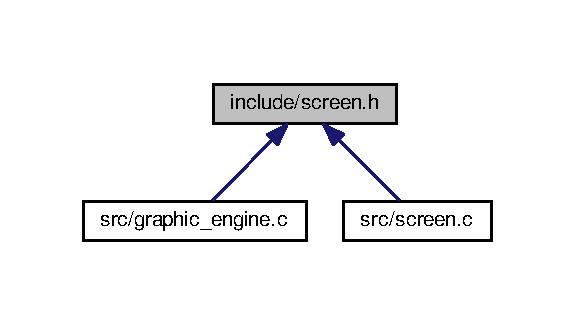
\includegraphics[width=276pt]{screen_8h__dep__incl}
\end{center}
\end{figure}
\subsection*{Macros}
\begin{DoxyCompactItemize}
\item 
\#define \hyperlink{screen_8h_aab63df3ae7b979d59ea0188055ea0763}{S\+C\+R\+E\+E\+N\+\_\+\+M\+A\+X\+\_\+\+S\+TR}~80
\end{DoxyCompactItemize}
\subsection*{Typedefs}
\begin{DoxyCompactItemize}
\item 
typedef struct \hyperlink{struct__Area}{\+\_\+\+Area} \hyperlink{screen_8h_acfdfc42f6522d75fa3c16713afde8127}{Area}
\begin{DoxyCompactList}\small\item\em screen of the game \end{DoxyCompactList}\end{DoxyCompactItemize}
\subsection*{Functions}
\begin{DoxyCompactItemize}
\item 
void \hyperlink{screen_8h_a9dbb6c251337c03c078dc330caee48d2}{screen\+\_\+init} ()
\begin{DoxyCompactList}\small\item\em initialises a new screen \end{DoxyCompactList}\item 
void \hyperlink{screen_8h_a3d6d82dde2bb4f3ddc4d276dabe313ef}{screen\+\_\+destroy} ()
\begin{DoxyCompactList}\small\item\em frees memory \end{DoxyCompactList}\item 
void \hyperlink{screen_8h_a3eaa0547a956d39b6c55c9593524e0d1}{screen\+\_\+paint} ()
\begin{DoxyCompactList}\small\item\em paints the screen \end{DoxyCompactList}\item 
void \hyperlink{screen_8h_a57b2f852be623dca59255306c1482eb2}{screen\+\_\+gets} (char $\ast$str)
\begin{DoxyCompactList}\small\item\em gets the data \end{DoxyCompactList}\item 
\hyperlink{screen_8h_acfdfc42f6522d75fa3c16713afde8127}{Area} $\ast$ \hyperlink{screen_8h_a194528bec3ed3b57618a8f2df9bea743}{screen\+\_\+area\+\_\+init} (int x, int y, int width, int height)
\begin{DoxyCompactList}\small\item\em creates new area \end{DoxyCompactList}\item 
void \hyperlink{screen_8h_aca5123ed5a7afb75e79c0001e5d1df4f}{screen\+\_\+area\+\_\+destroy} (\hyperlink{screen_8h_acfdfc42f6522d75fa3c16713afde8127}{Area} $\ast$area)
\begin{DoxyCompactList}\small\item\em frees memory \end{DoxyCompactList}\item 
void \hyperlink{screen_8h_a0950dc68cba3d491b909a8abaac1c666}{screen\+\_\+area\+\_\+clear} (\hyperlink{screen_8h_acfdfc42f6522d75fa3c16713afde8127}{Area} $\ast$area)
\begin{DoxyCompactList}\small\item\em clears the area \end{DoxyCompactList}\item 
void \hyperlink{screen_8h_af77fa9df4f7170e1e3bf1c6209b7f0c2}{screen\+\_\+area\+\_\+reset\+\_\+cursor} (\hyperlink{screen_8h_acfdfc42f6522d75fa3c16713afde8127}{Area} $\ast$area)
\begin{DoxyCompactList}\small\item\em resets cursor \end{DoxyCompactList}\item 
void \hyperlink{screen_8h_a4f4cd4c7899c096d6c90cc33de9a9814}{screen\+\_\+area\+\_\+puts} (\hyperlink{screen_8h_acfdfc42f6522d75fa3c16713afde8127}{Area} $\ast$area, char $\ast$str)
\begin{DoxyCompactList}\small\item\em puts area \end{DoxyCompactList}\end{DoxyCompactItemize}


\subsection{Detailed Description}
Defines the screen. 

Composes the screen of the game which is the visual part where we will be seeing every element of the game.

\begin{DoxyAuthor}{Author}
Andrés Mena 
\end{DoxyAuthor}
\begin{DoxyVersion}{Version}
1.\+1 
\end{DoxyVersion}
\begin{DoxyDate}{Date}
08-\/04-\/2018 
\end{DoxyDate}


\subsection{Macro Definition Documentation}
\index{screen.\+h@{screen.\+h}!S\+C\+R\+E\+E\+N\+\_\+\+M\+A\+X\+\_\+\+S\+TR@{S\+C\+R\+E\+E\+N\+\_\+\+M\+A\+X\+\_\+\+S\+TR}}
\index{S\+C\+R\+E\+E\+N\+\_\+\+M\+A\+X\+\_\+\+S\+TR@{S\+C\+R\+E\+E\+N\+\_\+\+M\+A\+X\+\_\+\+S\+TR}!screen.\+h@{screen.\+h}}
\subsubsection[{\texorpdfstring{S\+C\+R\+E\+E\+N\+\_\+\+M\+A\+X\+\_\+\+S\+TR}{SCREEN_MAX_STR}}]{\setlength{\rightskip}{0pt plus 5cm}\#define S\+C\+R\+E\+E\+N\+\_\+\+M\+A\+X\+\_\+\+S\+TR~80}\hypertarget{screen_8h_aab63df3ae7b979d59ea0188055ea0763}{}\label{screen_8h_aab63df3ae7b979d59ea0188055ea0763}
max str of the screen 

\subsection{Typedef Documentation}
\index{screen.\+h@{screen.\+h}!Area@{Area}}
\index{Area@{Area}!screen.\+h@{screen.\+h}}
\subsubsection[{\texorpdfstring{Area}{Area}}]{\setlength{\rightskip}{0pt plus 5cm}typedef struct {\bf \+\_\+\+Area} {\bf Area}}\hypertarget{screen_8h_acfdfc42f6522d75fa3c16713afde8127}{}\label{screen_8h_acfdfc42f6522d75fa3c16713afde8127}


screen of the game 

Struct for storing the variables that compose the screen of the game. 

\subsection{Function Documentation}
\index{screen.\+h@{screen.\+h}!screen\+\_\+area\+\_\+clear@{screen\+\_\+area\+\_\+clear}}
\index{screen\+\_\+area\+\_\+clear@{screen\+\_\+area\+\_\+clear}!screen.\+h@{screen.\+h}}
\subsubsection[{\texorpdfstring{screen\+\_\+area\+\_\+clear(\+Area $\ast$area)}{screen_area_clear(Area *area)}}]{\setlength{\rightskip}{0pt plus 5cm}void screen\+\_\+area\+\_\+clear (
\begin{DoxyParamCaption}
\item[{{\bf Area} $\ast$}]{area}
\end{DoxyParamCaption}
)}\hypertarget{screen_8h_a0950dc68cba3d491b909a8abaac1c666}{}\label{screen_8h_a0950dc68cba3d491b909a8abaac1c666}


clears the area 

Deletes everthing in the area, leaving it as if it was just created.

\begin{DoxyAuthor}{Author}
Andrés Mena 
\end{DoxyAuthor}

\begin{DoxyParams}{Parameters}
{\em area} & pointer to area. \\
\hline
\end{DoxyParams}
\begin{DoxyReturn}{Returns}
void. 
\end{DoxyReturn}
\index{screen.\+h@{screen.\+h}!screen\+\_\+area\+\_\+destroy@{screen\+\_\+area\+\_\+destroy}}
\index{screen\+\_\+area\+\_\+destroy@{screen\+\_\+area\+\_\+destroy}!screen.\+h@{screen.\+h}}
\subsubsection[{\texorpdfstring{screen\+\_\+area\+\_\+destroy(\+Area $\ast$area)}{screen_area_destroy(Area *area)}}]{\setlength{\rightskip}{0pt plus 5cm}void screen\+\_\+area\+\_\+destroy (
\begin{DoxyParamCaption}
\item[{{\bf Area} $\ast$}]{area}
\end{DoxyParamCaption}
)}\hypertarget{screen_8h_aca5123ed5a7afb75e79c0001e5d1df4f}{}\label{screen_8h_aca5123ed5a7afb75e79c0001e5d1df4f}


frees memory 

Receives pointer to area and frees the memory it occupied.

\begin{DoxyAuthor}{Author}
Andrés Mena 
\end{DoxyAuthor}

\begin{DoxyParams}{Parameters}
{\em area} & pointer to area. \\
\hline
\end{DoxyParams}
\begin{DoxyReturn}{Returns}
void. 
\end{DoxyReturn}
\index{screen.\+h@{screen.\+h}!screen\+\_\+area\+\_\+init@{screen\+\_\+area\+\_\+init}}
\index{screen\+\_\+area\+\_\+init@{screen\+\_\+area\+\_\+init}!screen.\+h@{screen.\+h}}
\subsubsection[{\texorpdfstring{screen\+\_\+area\+\_\+init(int x, int y, int width, int height)}{screen_area_init(int x, int y, int width, int height)}}]{\setlength{\rightskip}{0pt plus 5cm}{\bf Area}$\ast$ screen\+\_\+area\+\_\+init (
\begin{DoxyParamCaption}
\item[{int}]{x, }
\item[{int}]{y, }
\item[{int}]{width, }
\item[{int}]{height}
\end{DoxyParamCaption}
)}\hypertarget{screen_8h_a194528bec3ed3b57618a8f2df9bea743}{}\label{screen_8h_a194528bec3ed3b57618a8f2df9bea743}


creates new area 

Allocates memory for an area, using x and y coordinates as a start point and width and height as the size.

\begin{DoxyAuthor}{Author}
Andrés Mena 
\end{DoxyAuthor}

\begin{DoxyParams}{Parameters}
{\em x} & int (coord x). \\
\hline
{\em y} & int (coord y). \\
\hline
{\em width} & int (width of the area). \\
\hline
{\em height} & int (height of the area). \\
\hline
\end{DoxyParams}
\begin{DoxyReturn}{Returns}
pointer to area. 
\end{DoxyReturn}
\index{screen.\+h@{screen.\+h}!screen\+\_\+area\+\_\+puts@{screen\+\_\+area\+\_\+puts}}
\index{screen\+\_\+area\+\_\+puts@{screen\+\_\+area\+\_\+puts}!screen.\+h@{screen.\+h}}
\subsubsection[{\texorpdfstring{screen\+\_\+area\+\_\+puts(\+Area $\ast$area, char $\ast$str)}{screen_area_puts(Area *area, char *str)}}]{\setlength{\rightskip}{0pt plus 5cm}void screen\+\_\+area\+\_\+puts (
\begin{DoxyParamCaption}
\item[{{\bf Area} $\ast$}]{area, }
\item[{char $\ast$}]{str}
\end{DoxyParamCaption}
)}\hypertarget{screen_8h_a4f4cd4c7899c096d6c90cc33de9a9814}{}\label{screen_8h_a4f4cd4c7899c096d6c90cc33de9a9814}


puts area 

Starts a new line in the area.

\begin{DoxyAuthor}{Author}
Andrés Mena 
\end{DoxyAuthor}

\begin{DoxyParams}{Parameters}
{\em area} & pointer to area. \\
\hline
{\em str} & char. \\
\hline
\end{DoxyParams}
\begin{DoxyReturn}{Returns}
void. 
\end{DoxyReturn}
\index{screen.\+h@{screen.\+h}!screen\+\_\+area\+\_\+reset\+\_\+cursor@{screen\+\_\+area\+\_\+reset\+\_\+cursor}}
\index{screen\+\_\+area\+\_\+reset\+\_\+cursor@{screen\+\_\+area\+\_\+reset\+\_\+cursor}!screen.\+h@{screen.\+h}}
\subsubsection[{\texorpdfstring{screen\+\_\+area\+\_\+reset\+\_\+cursor(\+Area $\ast$area)}{screen_area_reset_cursor(Area *area)}}]{\setlength{\rightskip}{0pt plus 5cm}void screen\+\_\+area\+\_\+reset\+\_\+cursor (
\begin{DoxyParamCaption}
\item[{{\bf Area} $\ast$}]{area}
\end{DoxyParamCaption}
)}\hypertarget{screen_8h_af77fa9df4f7170e1e3bf1c6209b7f0c2}{}\label{screen_8h_af77fa9df4f7170e1e3bf1c6209b7f0c2}


resets cursor 

Resets the cursor, leaving it in the 0,0 coordinates of the area.

\begin{DoxyAuthor}{Author}
Andrés Mena 
\end{DoxyAuthor}

\begin{DoxyParams}{Parameters}
{\em area} & pointer to area. \\
\hline
\end{DoxyParams}
\begin{DoxyReturn}{Returns}
void. 
\end{DoxyReturn}
\index{screen.\+h@{screen.\+h}!screen\+\_\+destroy@{screen\+\_\+destroy}}
\index{screen\+\_\+destroy@{screen\+\_\+destroy}!screen.\+h@{screen.\+h}}
\subsubsection[{\texorpdfstring{screen\+\_\+destroy()}{screen_destroy()}}]{\setlength{\rightskip}{0pt plus 5cm}void screen\+\_\+destroy (
\begin{DoxyParamCaption}
{}
\end{DoxyParamCaption}
)}\hypertarget{screen_8h_a3d6d82dde2bb4f3ddc4d276dabe313ef}{}\label{screen_8h_a3d6d82dde2bb4f3ddc4d276dabe313ef}


frees memory 

frees the data that screen occupied.

\begin{DoxyAuthor}{Author}
Andrés Mena 
\end{DoxyAuthor}
\begin{DoxyReturn}{Returns}
void. 
\end{DoxyReturn}
\index{screen.\+h@{screen.\+h}!screen\+\_\+gets@{screen\+\_\+gets}}
\index{screen\+\_\+gets@{screen\+\_\+gets}!screen.\+h@{screen.\+h}}
\subsubsection[{\texorpdfstring{screen\+\_\+gets(char $\ast$str)}{screen_gets(char *str)}}]{\setlength{\rightskip}{0pt plus 5cm}void screen\+\_\+gets (
\begin{DoxyParamCaption}
\item[{char $\ast$}]{str}
\end{DoxyParamCaption}
)}\hypertarget{screen_8h_a57b2f852be623dca59255306c1482eb2}{}\label{screen_8h_a57b2f852be623dca59255306c1482eb2}


gets the data 

Gets the data typed in the ingame console (commands).

\begin{DoxyAuthor}{Author}
Andrés Mena 
\end{DoxyAuthor}

\begin{DoxyParams}{Parameters}
{\em str} & char (data of the console). \\
\hline
\end{DoxyParams}
\begin{DoxyReturn}{Returns}
void. 
\end{DoxyReturn}
\index{screen.\+h@{screen.\+h}!screen\+\_\+init@{screen\+\_\+init}}
\index{screen\+\_\+init@{screen\+\_\+init}!screen.\+h@{screen.\+h}}
\subsubsection[{\texorpdfstring{screen\+\_\+init()}{screen_init()}}]{\setlength{\rightskip}{0pt plus 5cm}void screen\+\_\+init (
\begin{DoxyParamCaption}
{}
\end{DoxyParamCaption}
)}\hypertarget{screen_8h_a9dbb6c251337c03c078dc330caee48d2}{}\label{screen_8h_a9dbb6c251337c03c078dc330caee48d2}


initialises a new screen 

Destroys any previous screen and allocates memory for a new one.

\begin{DoxyAuthor}{Author}
Andrés Mena 
\end{DoxyAuthor}
\begin{DoxyReturn}{Returns}
void. 
\end{DoxyReturn}
\index{screen.\+h@{screen.\+h}!screen\+\_\+paint@{screen\+\_\+paint}}
\index{screen\+\_\+paint@{screen\+\_\+paint}!screen.\+h@{screen.\+h}}
\subsubsection[{\texorpdfstring{screen\+\_\+paint()}{screen_paint()}}]{\setlength{\rightskip}{0pt plus 5cm}void screen\+\_\+paint (
\begin{DoxyParamCaption}
{}
\end{DoxyParamCaption}
)}\hypertarget{screen_8h_a3eaa0547a956d39b6c55c9593524e0d1}{}\label{screen_8h_a3eaa0547a956d39b6c55c9593524e0d1}


paints the screen 

Prints a screen in the console.

\begin{DoxyAuthor}{Author}
Andrés Mena 
\end{DoxyAuthor}
\begin{DoxyReturn}{Returns}
void. 
\end{DoxyReturn}

\hypertarget{set_8h}{}\section{include/set.h File Reference}
\label{set_8h}\index{include/set.\+h@{include/set.\+h}}


helps us manage other modules with a better organisation using its functions to change values.  


{\ttfamily \#include \char`\"{}types.\+h\char`\"{}}\\*
Include dependency graph for set.\+h\+:
\nopagebreak
\begin{figure}[H]
\begin{center}
\leavevmode
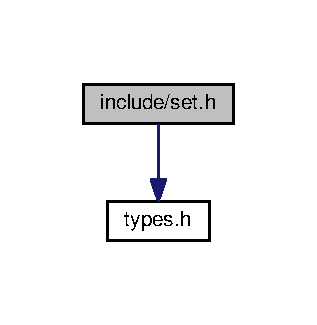
\includegraphics[width=152pt]{set_8h__incl}
\end{center}
\end{figure}
This graph shows which files directly or indirectly include this file\+:
\nopagebreak
\begin{figure}[H]
\begin{center}
\leavevmode
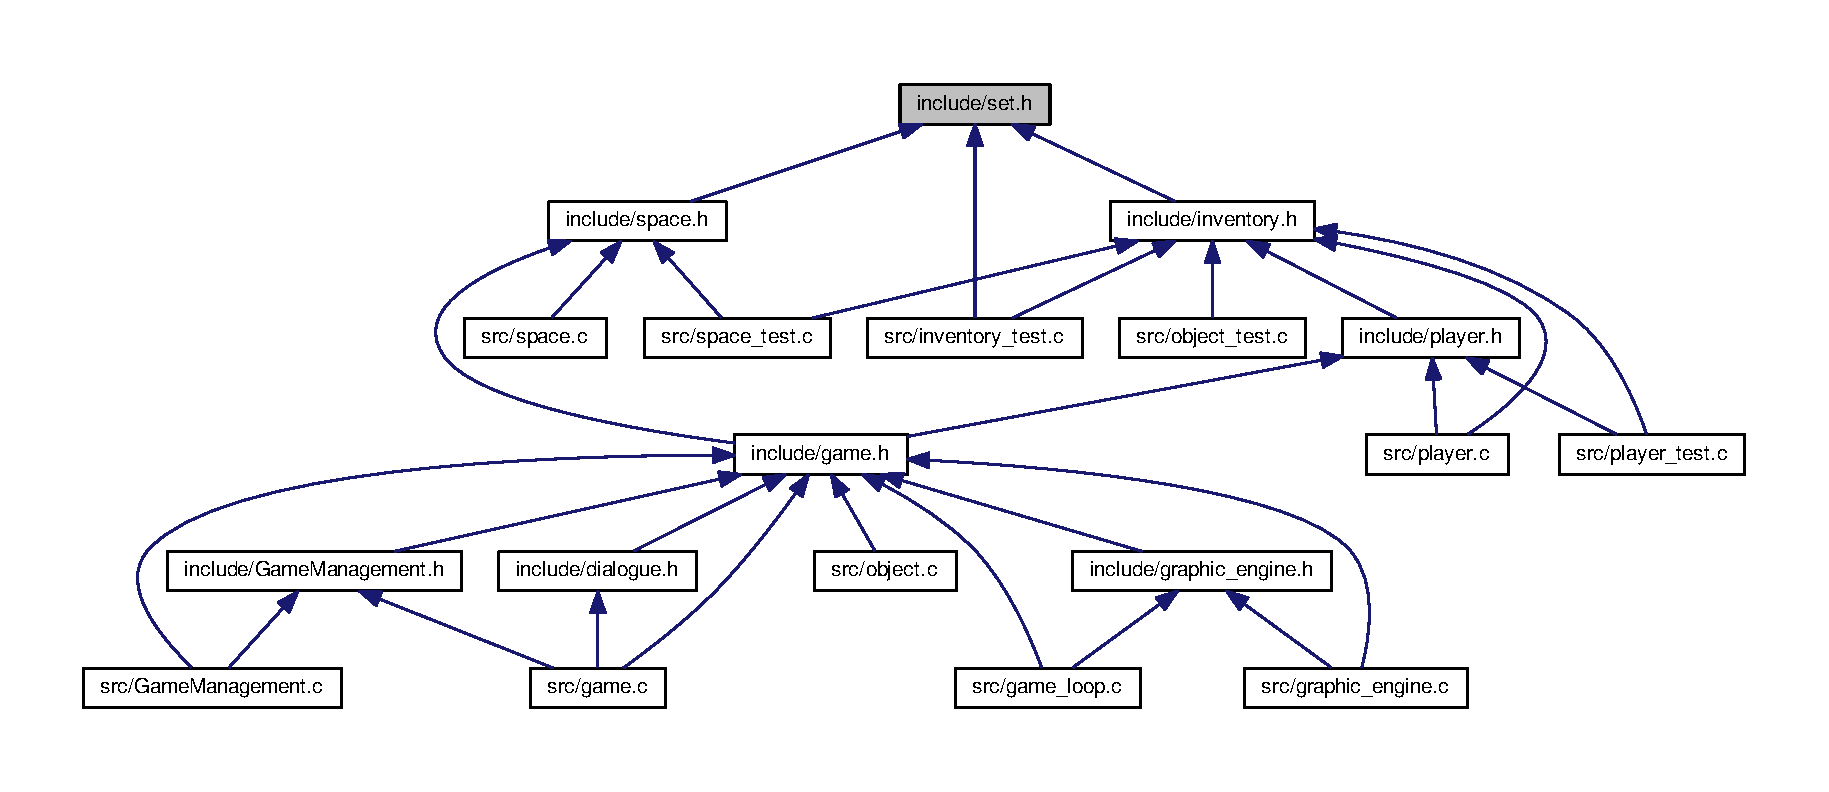
\includegraphics[width=350pt]{set_8h__dep__incl}
\end{center}
\end{figure}
\subsection*{Typedefs}
\begin{DoxyCompactItemize}
\item 
typedef struct \hyperlink{struct__Set}{\+\_\+\+Set} \hyperlink{set_8h_a6d3b7f7c92cbb4577ef3ef7ddbf93161}{Set}
\begin{DoxyCompactList}\small\item\em id and number of ids \end{DoxyCompactList}\end{DoxyCompactItemize}
\subsection*{Functions}
\begin{DoxyCompactItemize}
\item 
\hyperlink{set_8h_a6d3b7f7c92cbb4577ef3ef7ddbf93161}{Set} $\ast$ \hyperlink{set_8h_abcc73b7ad3913fc92dd95d366c9c8687}{set\+\_\+create} ()
\begin{DoxyCompactList}\small\item\em creates a set \end{DoxyCompactList}\item 
void \hyperlink{set_8h_a9d762a027f1c3bcdd22f70ee9093a7dd}{set\+\_\+destroy} (\hyperlink{set_8h_a6d3b7f7c92cbb4577ef3ef7ddbf93161}{Set} $\ast$set)
\begin{DoxyCompactList}\small\item\em frees memory \end{DoxyCompactList}\item 
\hyperlink{types_8h_a32c27cc471df37f4fc818d65de0a56c4}{S\+T\+A\+T\+US} \hyperlink{set_8h_ab464b368bff979f29376f9b85675e547}{set\+\_\+add\+\_\+value} (\hyperlink{types_8h_a845e604fb28f7e3d97549da3448149d3}{Id} id, \hyperlink{set_8h_a6d3b7f7c92cbb4577ef3ef7ddbf93161}{Set} $\ast$set)
\begin{DoxyCompactList}\small\item\em adds a value defined by the set \end{DoxyCompactList}\item 
\hyperlink{types_8h_a32c27cc471df37f4fc818d65de0a56c4}{S\+T\+A\+T\+US} \hyperlink{set_8h_ad46a5d9be2d890c89866723df02d39ef}{set\+\_\+delete\+\_\+value} (\hyperlink{types_8h_a845e604fb28f7e3d97549da3448149d3}{Id} id, \hyperlink{set_8h_a6d3b7f7c92cbb4577ef3ef7ddbf93161}{Set} $\ast$set)
\begin{DoxyCompactList}\small\item\em deletes a value already defined \end{DoxyCompactList}\item 
int \hyperlink{set_8h_a844c749b0d18e9a97156a8aa9caabcd9}{set\+\_\+get\+\_\+nids} (\hyperlink{set_8h_a6d3b7f7c92cbb4577ef3ef7ddbf93161}{Set} $\ast$set)
\begin{DoxyCompactList}\small\item\em gets the number of ids \end{DoxyCompactList}\item 
\hyperlink{types_8h_a845e604fb28f7e3d97549da3448149d3}{Id} \hyperlink{set_8h_a319cad66db01db8729d86139a9743aa4}{get\+\_\+set} (\hyperlink{set_8h_a6d3b7f7c92cbb4577ef3ef7ddbf93161}{Set} $\ast$set, int position)
\begin{DoxyCompactList}\small\item\em gets an id using a set \end{DoxyCompactList}\item 
\hyperlink{types_8h_a3e5b8192e7d9ffaf3542f1210aec18dd}{B\+O\+OL} \hyperlink{set_8h_a796847f6bc6d359fd8e757323b30514a}{set\+\_\+has\+\_\+id} (\hyperlink{set_8h_a6d3b7f7c92cbb4577ef3ef7ddbf93161}{Set} $\ast$set, \hyperlink{types_8h_a845e604fb28f7e3d97549da3448149d3}{Id} id)
\begin{DoxyCompactList}\small\item\em checks the id of a set \end{DoxyCompactList}\item 
void \hyperlink{set_8h_a1c41ccff75cd22c0bd739b3cc61f16b9}{set\+\_\+print\+\_\+values} (\hyperlink{set_8h_a6d3b7f7c92cbb4577ef3ef7ddbf93161}{Set} $\ast$set)
\begin{DoxyCompactList}\small\item\em Prints a list with the ids of the elements of a list. \end{DoxyCompactList}\end{DoxyCompactItemize}


\subsection{Detailed Description}
helps us manage other modules with a better organisation using its functions to change values. 

The functions of the set module, will help us in other modules. By using the functions of this module, we will be able to modify and change values such as the id of an object and we will be able to do it in a more organised way.

\begin{DoxyAuthor}{Author}
Juan Moreno 
\end{DoxyAuthor}
\begin{DoxyVersion}{Version}
2.\+0 
\end{DoxyVersion}
\begin{DoxyDate}{Date}
05-\/04-\/2018 
\end{DoxyDate}


\subsection{Typedef Documentation}
\index{set.\+h@{set.\+h}!Set@{Set}}
\index{Set@{Set}!set.\+h@{set.\+h}}
\subsubsection[{\texorpdfstring{Set}{Set}}]{\setlength{\rightskip}{0pt plus 5cm}typedef struct {\bf \+\_\+\+Set} {\bf Set}}\hypertarget{set_8h_a6d3b7f7c92cbb4577ef3ef7ddbf93161}{}\label{set_8h_a6d3b7f7c92cbb4577ef3ef7ddbf93161}


id and number of ids 

Struct for managing the values and adding ids by using an id and the number of ids. 

\subsection{Function Documentation}
\index{set.\+h@{set.\+h}!get\+\_\+set@{get\+\_\+set}}
\index{get\+\_\+set@{get\+\_\+set}!set.\+h@{set.\+h}}
\subsubsection[{\texorpdfstring{get\+\_\+set(\+Set $\ast$set, int position)}{get_set(Set *set, int position)}}]{\setlength{\rightskip}{0pt plus 5cm}{\bf Id} get\+\_\+set (
\begin{DoxyParamCaption}
\item[{{\bf Set} $\ast$}]{set, }
\item[{int}]{position}
\end{DoxyParamCaption}
)}\hypertarget{set_8h_a319cad66db01db8729d86139a9743aa4}{}\label{set_8h_a319cad66db01db8729d86139a9743aa4}


gets an id using a set 

Function in which the Id of the object in a received position is returned.

\begin{DoxyAuthor}{Author}
Juan Moreno 
\end{DoxyAuthor}

\begin{DoxyParams}{Parameters}
{\em set} & pointer to set. \\
\hline
{\em position} & position of the set(int). \\
\hline
\end{DoxyParams}
\begin{DoxyReturn}{Returns}
Id, N\+O\+\_\+\+ID if set is pointing N\+U\+LL. 
\end{DoxyReturn}
\index{set.\+h@{set.\+h}!set\+\_\+add\+\_\+value@{set\+\_\+add\+\_\+value}}
\index{set\+\_\+add\+\_\+value@{set\+\_\+add\+\_\+value}!set.\+h@{set.\+h}}
\subsubsection[{\texorpdfstring{set\+\_\+add\+\_\+value(\+Id id, Set $\ast$set)}{set_add_value(Id id, Set *set)}}]{\setlength{\rightskip}{0pt plus 5cm}{\bf S\+T\+A\+T\+US} set\+\_\+add\+\_\+value (
\begin{DoxyParamCaption}
\item[{{\bf Id}}]{id, }
\item[{{\bf Set} $\ast$}]{set}
\end{DoxyParamCaption}
)}\hypertarget{set_8h_ab464b368bff979f29376f9b85675e547}{}\label{set_8h_ab464b368bff979f29376f9b85675e547}


adds a value defined by the set 

It is the function in charge of adding sets to other functions that require it.

\begin{DoxyAuthor}{Author}
Juan Moreno 
\end{DoxyAuthor}

\begin{DoxyParams}{Parameters}
{\em id} & (long int). \\
\hline
{\em set} & pointer to set. \\
\hline
\end{DoxyParams}
\begin{DoxyReturn}{Returns}
S\+T\+A\+T\+US, E\+R\+R\+OR if argument received is N\+U\+LL, if not, OK. 
\end{DoxyReturn}
\index{set.\+h@{set.\+h}!set\+\_\+create@{set\+\_\+create}}
\index{set\+\_\+create@{set\+\_\+create}!set.\+h@{set.\+h}}
\subsubsection[{\texorpdfstring{set\+\_\+create()}{set_create()}}]{\setlength{\rightskip}{0pt plus 5cm}{\bf Set}$\ast$ set\+\_\+create (
\begin{DoxyParamCaption}
{}
\end{DoxyParamCaption}
)}\hypertarget{set_8h_abcc73b7ad3913fc92dd95d366c9c8687}{}\label{set_8h_abcc73b7ad3913fc92dd95d366c9c8687}


creates a set 

It creates a new set, if id is -\/1(N\+O\+\_\+\+ID), N\+U\+LL is returned, if not, memory for a new set is reserved and created. If anything goes wrong, it returns N\+U\+LL.

\begin{DoxyAuthor}{Author}
Juan Moreno 
\end{DoxyAuthor}
\begin{DoxyReturn}{Returns}
Pointer to set, N\+U\+LL if something goes wrong. 
\end{DoxyReturn}
\index{set.\+h@{set.\+h}!set\+\_\+delete\+\_\+value@{set\+\_\+delete\+\_\+value}}
\index{set\+\_\+delete\+\_\+value@{set\+\_\+delete\+\_\+value}!set.\+h@{set.\+h}}
\subsubsection[{\texorpdfstring{set\+\_\+delete\+\_\+value(\+Id id, Set $\ast$set)}{set_delete_value(Id id, Set *set)}}]{\setlength{\rightskip}{0pt plus 5cm}{\bf S\+T\+A\+T\+US} set\+\_\+delete\+\_\+value (
\begin{DoxyParamCaption}
\item[{{\bf Id}}]{id, }
\item[{{\bf Set} $\ast$}]{set}
\end{DoxyParamCaption}
)}\hypertarget{set_8h_ad46a5d9be2d890c89866723df02d39ef}{}\label{set_8h_ad46a5d9be2d890c89866723df02d39ef}


deletes a value already defined 

Function in charge of deleting sets when you are willing to do it and when it is necessary.

\begin{DoxyAuthor}{Author}
Juan Moreno 
\end{DoxyAuthor}

\begin{DoxyParams}{Parameters}
{\em id} & long int. \\
\hline
{\em set} & pointer to set. \\
\hline
\end{DoxyParams}
\begin{DoxyReturn}{Returns}
S\+T\+A\+T\+US, E\+R\+R\+OR if argument received is N\+U\+LL, if not, OK. 
\end{DoxyReturn}
\index{set.\+h@{set.\+h}!set\+\_\+destroy@{set\+\_\+destroy}}
\index{set\+\_\+destroy@{set\+\_\+destroy}!set.\+h@{set.\+h}}
\subsubsection[{\texorpdfstring{set\+\_\+destroy(\+Set $\ast$set)}{set_destroy(Set *set)}}]{\setlength{\rightskip}{0pt plus 5cm}void set\+\_\+destroy (
\begin{DoxyParamCaption}
\item[{{\bf Set} $\ast$}]{set}
\end{DoxyParamCaption}
)}\hypertarget{set_8h_a9d762a027f1c3bcdd22f70ee9093a7dd}{}\label{set_8h_a9d762a027f1c3bcdd22f70ee9093a7dd}


frees memory 

Receives pointer to set and frees the memory it occupied.

\begin{DoxyAuthor}{Author}
Juan Moreno 
\end{DoxyAuthor}

\begin{DoxyParams}{Parameters}
{\em set} & pointer to set. \\
\hline
\end{DoxyParams}
\begin{DoxyReturn}{Returns}
V\+O\+ID F\+U\+N\+C\+T\+I\+ON T\+Y\+PE. 
\end{DoxyReturn}
\index{set.\+h@{set.\+h}!set\+\_\+get\+\_\+nids@{set\+\_\+get\+\_\+nids}}
\index{set\+\_\+get\+\_\+nids@{set\+\_\+get\+\_\+nids}!set.\+h@{set.\+h}}
\subsubsection[{\texorpdfstring{set\+\_\+get\+\_\+nids(\+Set $\ast$set)}{set_get_nids(Set *set)}}]{\setlength{\rightskip}{0pt plus 5cm}int set\+\_\+get\+\_\+nids (
\begin{DoxyParamCaption}
\item[{{\bf Set} $\ast$}]{set}
\end{DoxyParamCaption}
)}\hypertarget{set_8h_a844c749b0d18e9a97156a8aa9caabcd9}{}\label{set_8h_a844c749b0d18e9a97156a8aa9caabcd9}


gets the number of ids 

Function in charge of returning the number of ids by using that will be used when considered useful and convenient.

\begin{DoxyAuthor}{Author}
Juan Moreno 
\end{DoxyAuthor}

\begin{DoxyParams}{Parameters}
{\em set} & pointer to set. \\
\hline
\end{DoxyParams}
\begin{DoxyReturn}{Returns}
pointer to set (int) referring to the number of ids. 
\end{DoxyReturn}
\index{set.\+h@{set.\+h}!set\+\_\+has\+\_\+id@{set\+\_\+has\+\_\+id}}
\index{set\+\_\+has\+\_\+id@{set\+\_\+has\+\_\+id}!set.\+h@{set.\+h}}
\subsubsection[{\texorpdfstring{set\+\_\+has\+\_\+id(\+Set $\ast$set, Id id)}{set_has_id(Set *set, Id id)}}]{\setlength{\rightskip}{0pt plus 5cm}{\bf B\+O\+OL} set\+\_\+has\+\_\+id (
\begin{DoxyParamCaption}
\item[{{\bf Set} $\ast$}]{set, }
\item[{{\bf Id}}]{id}
\end{DoxyParamCaption}
)}\hypertarget{set_8h_a796847f6bc6d359fd8e757323b30514a}{}\label{set_8h_a796847f6bc6d359fd8e757323b30514a}


checks the id of a set 

It is the function that will be used in other modules to check if that function is using an id by passing two arguments\+: a pointer to set and an id.

\begin{DoxyAuthor}{Author}
Juan Moreno 
\end{DoxyAuthor}

\begin{DoxyParams}{Parameters}
{\em set} & pointer to set. \\
\hline
{\em id} & long int. \\
\hline
\end{DoxyParams}
\begin{DoxyReturn}{Returns}
B\+O\+OL, F\+A\+L\+SE if when checking is not correct, if it is correct, T\+R\+UE. 
\end{DoxyReturn}
\index{set.\+h@{set.\+h}!set\+\_\+print\+\_\+values@{set\+\_\+print\+\_\+values}}
\index{set\+\_\+print\+\_\+values@{set\+\_\+print\+\_\+values}!set.\+h@{set.\+h}}
\subsubsection[{\texorpdfstring{set\+\_\+print\+\_\+values(\+Set $\ast$set)}{set_print_values(Set *set)}}]{\setlength{\rightskip}{0pt plus 5cm}void set\+\_\+print\+\_\+values (
\begin{DoxyParamCaption}
\item[{{\bf Set} $\ast$}]{set}
\end{DoxyParamCaption}
)}\hypertarget{set_8h_a1c41ccff75cd22c0bd739b3cc61f16b9}{}\label{set_8h_a1c41ccff75cd22c0bd739b3cc61f16b9}


Prints a list with the ids of the elements of a list. 

Function in charge of printing the set, in order to check that everything is working correctly.

\begin{DoxyAuthor}{Author}
Juan Moreno 
\end{DoxyAuthor}

\begin{DoxyParams}{Parameters}
{\em set} & pointer to set. \\
\hline
\end{DoxyParams}
\begin{DoxyReturn}{Returns}
V\+O\+ID F\+U\+N\+C\+T\+I\+ON T\+Y\+PE, IT O\+N\+LY P\+R\+I\+N\+TS T\+HE L\+I\+NE WE O\+R\+D\+E\+R\+ED IT TO P\+R\+I\+NT. 
\end{DoxyReturn}

\hypertarget{space_8h}{}\section{include/space.h File Reference}
\label{space_8h}\index{include/space.\+h@{include/space.\+h}}


Defines the space related function.  


{\ttfamily \#include \char`\"{}types.\+h\char`\"{}}\\*
{\ttfamily \#include \char`\"{}object.\+h\char`\"{}}\\*
{\ttfamily \#include \char`\"{}set.\+h\char`\"{}}\\*
Include dependency graph for space.\+h\+:
\nopagebreak
\begin{figure}[H]
\begin{center}
\leavevmode
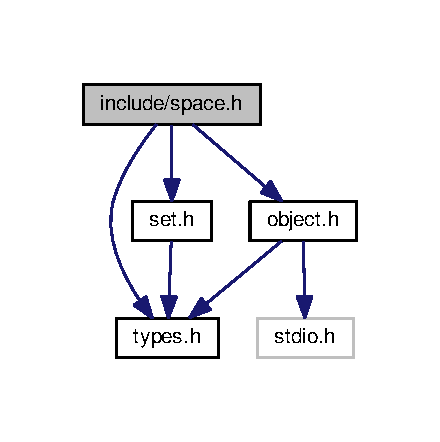
\includegraphics[width=211pt]{space_8h__incl}
\end{center}
\end{figure}
This graph shows which files directly or indirectly include this file\+:
\nopagebreak
\begin{figure}[H]
\begin{center}
\leavevmode
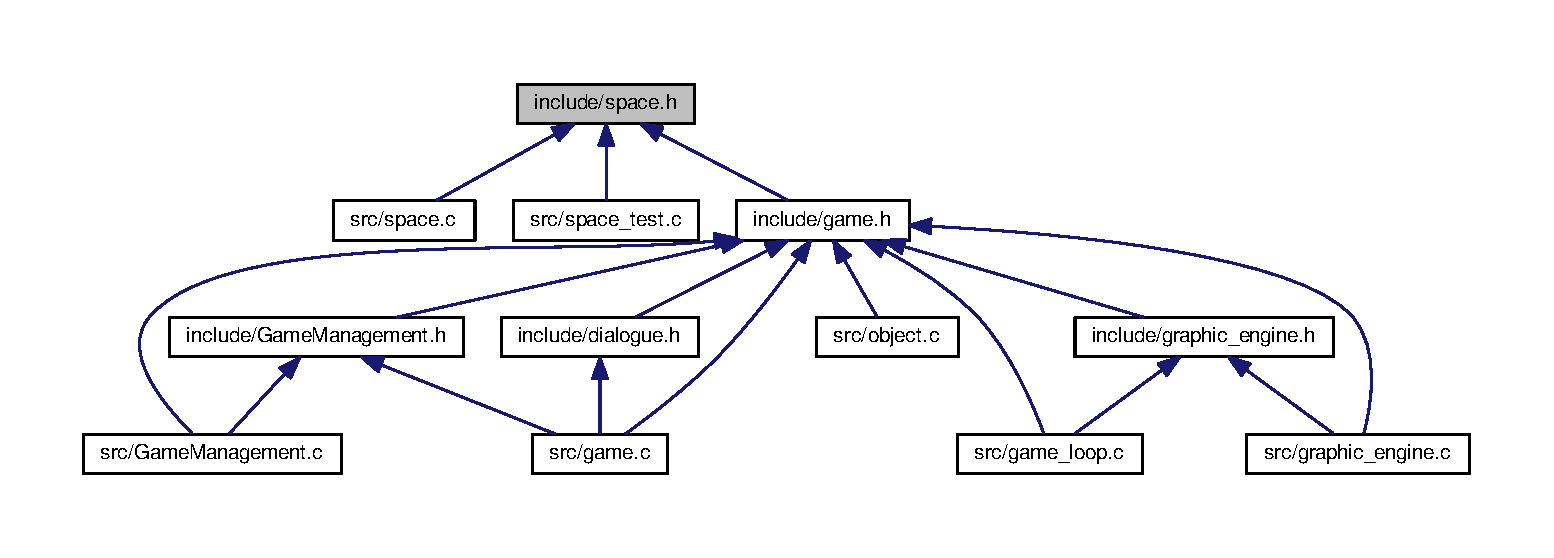
\includegraphics[width=350pt]{space_8h__dep__incl}
\end{center}
\end{figure}
\subsection*{Macros}
\begin{DoxyCompactItemize}
\item 
\#define \hyperlink{space_8h_a5f54fd55f983a2e33ce076cd9f587e82}{M\+A\+X\+\_\+\+S\+P\+A\+C\+ES}~100
\item 
\#define \hyperlink{space_8h_a088cbe7c6f78264d46c2624194c5c680}{F\+I\+R\+S\+T\+\_\+\+S\+P\+A\+CE}~1
\end{DoxyCompactItemize}
\subsection*{Typedefs}
\begin{DoxyCompactItemize}
\item 
typedef struct \hyperlink{struct__Space}{\+\_\+\+Space} \hyperlink{space_8h_a67533ffc2b70463baecc38fb0629bbfc}{Space}
\begin{DoxyCompactList}\small\item\em spaces of the game \end{DoxyCompactList}\end{DoxyCompactItemize}
\subsection*{Functions}
\begin{DoxyCompactItemize}
\item 
\hyperlink{space_8h_a67533ffc2b70463baecc38fb0629bbfc}{Space} $\ast$ \hyperlink{space_8h_a162866fcea156b800fd546d0ffd271c9}{space\+\_\+create} (\hyperlink{types_8h_a845e604fb28f7e3d97549da3448149d3}{Id} id)
\begin{DoxyCompactList}\small\item\em allocates memory for a new space \end{DoxyCompactList}\item 
\hyperlink{types_8h_a32c27cc471df37f4fc818d65de0a56c4}{S\+T\+A\+T\+US} \hyperlink{space_8h_a5c70c70398923693ddbe4dfac8d72a0d}{space\+\_\+destroy} (\hyperlink{space_8h_a67533ffc2b70463baecc38fb0629bbfc}{Space} $\ast$space)
\begin{DoxyCompactList}\small\item\em frees memory \end{DoxyCompactList}\item 
\hyperlink{types_8h_a845e604fb28f7e3d97549da3448149d3}{Id} \hyperlink{space_8h_ac8ddfd0d8692fd852ee49698c446cb50}{space\+\_\+get\+\_\+id} (\hyperlink{space_8h_a67533ffc2b70463baecc38fb0629bbfc}{Space} $\ast$space)
\begin{DoxyCompactList}\small\item\em gets the id of a space \end{DoxyCompactList}\item 
int \hyperlink{space_8h_ab39ec663cd2f64cd8406f5ba6f5493ea}{space\+\_\+get\+\_\+object\+\_\+number} (\hyperlink{space_8h_a67533ffc2b70463baecc38fb0629bbfc}{Space} $\ast$space)
\begin{DoxyCompactList}\small\item\em gets number \end{DoxyCompactList}\item 
\hyperlink{types_8h_a32c27cc471df37f4fc818d65de0a56c4}{S\+T\+A\+T\+US} \hyperlink{space_8h_aab5b468f9822ab78dbe16d1321870d93}{space\+\_\+set\+\_\+name} (\hyperlink{space_8h_a67533ffc2b70463baecc38fb0629bbfc}{Space} $\ast$space, char $\ast$name)
\begin{DoxyCompactList}\small\item\em sets the name of a space \end{DoxyCompactList}\item 
const char $\ast$ \hyperlink{space_8h_a310c540cd6e11073f7328add1f927001}{space\+\_\+get\+\_\+name} (\hyperlink{space_8h_a67533ffc2b70463baecc38fb0629bbfc}{Space} $\ast$space)
\begin{DoxyCompactList}\small\item\em gets the name of a space \end{DoxyCompactList}\item 
\hyperlink{types_8h_a32c27cc471df37f4fc818d65de0a56c4}{S\+T\+A\+T\+US} \hyperlink{space_8h_a9e6e3e3bac4996ac6b8bd555e52bfb26}{space\+\_\+set\+\_\+north} (\hyperlink{space_8h_a67533ffc2b70463baecc38fb0629bbfc}{Space} $\ast$space, \hyperlink{types_8h_a845e604fb28f7e3d97549da3448149d3}{Id} id)
\begin{DoxyCompactList}\small\item\em sets location of spaces \end{DoxyCompactList}\item 
\hyperlink{types_8h_a845e604fb28f7e3d97549da3448149d3}{Id} \hyperlink{space_8h_ad331fba774897900f615d9d2e8d81a90}{space\+\_\+get\+\_\+north} (\hyperlink{space_8h_a67533ffc2b70463baecc38fb0629bbfc}{Space} $\ast$space)
\begin{DoxyCompactList}\small\item\em gets location of spaces \end{DoxyCompactList}\item 
\hyperlink{types_8h_a32c27cc471df37f4fc818d65de0a56c4}{S\+T\+A\+T\+US} \hyperlink{space_8h_a422ab9f220b4c471c44256a27377de1a}{space\+\_\+set\+\_\+south} (\hyperlink{space_8h_a67533ffc2b70463baecc38fb0629bbfc}{Space} $\ast$space, \hyperlink{types_8h_a845e604fb28f7e3d97549da3448149d3}{Id} id)
\begin{DoxyCompactList}\small\item\em sets location of spaces \end{DoxyCompactList}\item 
\hyperlink{types_8h_a845e604fb28f7e3d97549da3448149d3}{Id} \hyperlink{space_8h_a9b86e1335c423eaad832e50d4c12cf1f}{space\+\_\+get\+\_\+south} (\hyperlink{space_8h_a67533ffc2b70463baecc38fb0629bbfc}{Space} $\ast$space)
\begin{DoxyCompactList}\small\item\em gets location of spaces \end{DoxyCompactList}\item 
\hyperlink{types_8h_a32c27cc471df37f4fc818d65de0a56c4}{S\+T\+A\+T\+US} \hyperlink{space_8h_a860a8f3e0227955ad56d1a12f0bdc44a}{space\+\_\+set\+\_\+east} (\hyperlink{space_8h_a67533ffc2b70463baecc38fb0629bbfc}{Space} $\ast$space, \hyperlink{types_8h_a845e604fb28f7e3d97549da3448149d3}{Id} id)
\begin{DoxyCompactList}\small\item\em sets location of spaces \end{DoxyCompactList}\item 
\hyperlink{types_8h_a845e604fb28f7e3d97549da3448149d3}{Id} \hyperlink{space_8h_a978a22b77f74bb2dab68a00571abbe0b}{space\+\_\+get\+\_\+east} (\hyperlink{space_8h_a67533ffc2b70463baecc38fb0629bbfc}{Space} $\ast$space)
\begin{DoxyCompactList}\small\item\em gets location of spaces \end{DoxyCompactList}\item 
\hyperlink{types_8h_a32c27cc471df37f4fc818d65de0a56c4}{S\+T\+A\+T\+US} \hyperlink{space_8h_ad44b14cb38902cf31fa1f341beaab0db}{space\+\_\+set\+\_\+west} (\hyperlink{space_8h_a67533ffc2b70463baecc38fb0629bbfc}{Space} $\ast$space, \hyperlink{types_8h_a845e604fb28f7e3d97549da3448149d3}{Id} id)
\begin{DoxyCompactList}\small\item\em sets location of spaces \end{DoxyCompactList}\item 
\hyperlink{types_8h_a845e604fb28f7e3d97549da3448149d3}{Id} \hyperlink{space_8h_af495ebfd5d13eba1a48cebd10992a17f}{space\+\_\+get\+\_\+west} (\hyperlink{space_8h_a67533ffc2b70463baecc38fb0629bbfc}{Space} $\ast$space)
\begin{DoxyCompactList}\small\item\em gets location of spaces \end{DoxyCompactList}\item 
\hyperlink{types_8h_a32c27cc471df37f4fc818d65de0a56c4}{S\+T\+A\+T\+US} \hyperlink{space_8h_a902da49e4ca892778f89a2722d52c45d}{space\+\_\+set\+\_\+gdesc1} (\hyperlink{space_8h_a67533ffc2b70463baecc38fb0629bbfc}{Space} $\ast$space, char $\ast$c)
\begin{DoxyCompactList}\small\item\em sets a graphic description \end{DoxyCompactList}\item 
char $\ast$ \hyperlink{space_8h_af3f47f8a1cbcad3fdeaf1d288afba10f}{space\+\_\+get\+\_\+gdesc1} (\hyperlink{space_8h_a67533ffc2b70463baecc38fb0629bbfc}{Space} $\ast$space)
\begin{DoxyCompactList}\small\item\em returns the graphic description \end{DoxyCompactList}\item 
\hyperlink{types_8h_a32c27cc471df37f4fc818d65de0a56c4}{S\+T\+A\+T\+US} \hyperlink{space_8h_af6117bf6bde9509f097257d98bd46970}{space\+\_\+set\+\_\+gdesc2} (\hyperlink{space_8h_a67533ffc2b70463baecc38fb0629bbfc}{Space} $\ast$space, char $\ast$c)
\begin{DoxyCompactList}\small\item\em sets a graphic description \end{DoxyCompactList}\item 
char $\ast$ \hyperlink{space_8h_a095abfb28adfae37d023160df0e3bf49}{space\+\_\+get\+\_\+gdesc2} (\hyperlink{space_8h_a67533ffc2b70463baecc38fb0629bbfc}{Space} $\ast$space)
\begin{DoxyCompactList}\small\item\em returns the graphic description \end{DoxyCompactList}\item 
\hyperlink{types_8h_a32c27cc471df37f4fc818d65de0a56c4}{S\+T\+A\+T\+US} \hyperlink{space_8h_a087794c057f78113c1e1cf007178f3ac}{space\+\_\+set\+\_\+gdesc3} (\hyperlink{space_8h_a67533ffc2b70463baecc38fb0629bbfc}{Space} $\ast$space, char $\ast$c)
\begin{DoxyCompactList}\small\item\em sets a graphic description \end{DoxyCompactList}\item 
char $\ast$ \hyperlink{space_8h_ae7ec02a0cd76f82599817fba31c5d912}{space\+\_\+get\+\_\+gdesc3} (\hyperlink{space_8h_a67533ffc2b70463baecc38fb0629bbfc}{Space} $\ast$space)
\begin{DoxyCompactList}\small\item\em returns the graphic description \end{DoxyCompactList}\item 
\hyperlink{types_8h_a32c27cc471df37f4fc818d65de0a56c4}{S\+T\+A\+T\+US} \hyperlink{space_8h_a97f27baaafef8eb986d167788dc84bec}{space\+\_\+set\+\_\+object} (\hyperlink{space_8h_a67533ffc2b70463baecc38fb0629bbfc}{Space} $\ast$space, \hyperlink{object_8h_a7f8bbcda919b65ce67f92fba08e0212f}{Object} $\ast$o)
\begin{DoxyCompactList}\small\item\em sets an object for a space \end{DoxyCompactList}\item 
\hyperlink{set_8h_a6d3b7f7c92cbb4577ef3ef7ddbf93161}{Set} $\ast$ \hyperlink{space_8h_ab24abae4e127bf0bca596cd71ba3aad6}{space\+\_\+get\+\_\+object} (\hyperlink{space_8h_a67533ffc2b70463baecc38fb0629bbfc}{Space} $\ast$space)
\begin{DoxyCompactList}\small\item\em gets an object from a space \end{DoxyCompactList}\item 
\hyperlink{types_8h_a32c27cc471df37f4fc818d65de0a56c4}{S\+T\+A\+T\+US} \hyperlink{space_8h_a52d48979efbb5ba49c0988ddffc33769}{space\+\_\+set\+\_\+short\+\_\+description} (\hyperlink{space_8h_a67533ffc2b70463baecc38fb0629bbfc}{Space} $\ast$space, char $\ast$description)
\begin{DoxyCompactList}\small\item\em sets description \end{DoxyCompactList}\item 
char $\ast$ \hyperlink{space_8h_aa389d6b22e635bb9d2f1a18d9cd0d1cb}{space\+\_\+get\+\_\+short\+\_\+description} (\hyperlink{space_8h_a67533ffc2b70463baecc38fb0629bbfc}{Space} $\ast$space)
\begin{DoxyCompactList}\small\item\em gets description \end{DoxyCompactList}\item 
\hyperlink{types_8h_a32c27cc471df37f4fc818d65de0a56c4}{S\+T\+A\+T\+US} \hyperlink{space_8h_adaea1c731830282c8a29f3477a93ac2e}{space\+\_\+set\+\_\+long\+\_\+description} (\hyperlink{space_8h_a67533ffc2b70463baecc38fb0629bbfc}{Space} $\ast$space, char $\ast$description)
\begin{DoxyCompactList}\small\item\em sets description \end{DoxyCompactList}\item 
char $\ast$ \hyperlink{space_8h_a5c38e8f0892b1683b4f058d17ea1549d}{space\+\_\+get\+\_\+long\+\_\+description} (\hyperlink{space_8h_a67533ffc2b70463baecc38fb0629bbfc}{Space} $\ast$space)
\begin{DoxyCompactList}\small\item\em gets description \end{DoxyCompactList}\item 
\hyperlink{types_8h_a32c27cc471df37f4fc818d65de0a56c4}{S\+T\+A\+T\+US} \hyperlink{space_8h_a18eca058da6cdf20ae5eda9d122d992e}{space\+\_\+print} (\hyperlink{space_8h_a67533ffc2b70463baecc38fb0629bbfc}{Space} $\ast$space)
\begin{DoxyCompactList}\small\item\em prints the spaces \end{DoxyCompactList}\item 
\hyperlink{types_8h_a32c27cc471df37f4fc818d65de0a56c4}{S\+T\+A\+T\+US} \hyperlink{space_8h_ab7c8deb146adb40f1c07660e5442650e}{space\+\_\+object\+\_\+destroy} (\hyperlink{space_8h_a67533ffc2b70463baecc38fb0629bbfc}{Space} $\ast$s, \hyperlink{types_8h_a845e604fb28f7e3d97549da3448149d3}{Id} id)
\begin{DoxyCompactList}\small\item\em frees memory \end{DoxyCompactList}\item 
\hyperlink{types_8h_a3e5b8192e7d9ffaf3542f1210aec18dd}{B\+O\+OL} \hyperlink{space_8h_a0642818ac93d8696fa46f371b8c2801d}{space\+\_\+is\+\_\+linked} (\hyperlink{space_8h_a67533ffc2b70463baecc38fb0629bbfc}{Space} $\ast$s)
\begin{DoxyCompactList}\small\item\em checks if space is linked \end{DoxyCompactList}\item 
\hyperlink{types_8h_a32c27cc471df37f4fc818d65de0a56c4}{S\+T\+A\+T\+US} \hyperlink{space_8h_ab2803dc6dee6ca4360860b0b9a66b34e}{space\+\_\+set\+\_\+iluminate} (\hyperlink{space_8h_a67533ffc2b70463baecc38fb0629bbfc}{Space} $\ast$space, \hyperlink{types_8h_a3e5b8192e7d9ffaf3542f1210aec18dd}{B\+O\+OL} iluminate)
\begin{DoxyCompactList}\small\item\em sets ilumination \end{DoxyCompactList}\item 
\hyperlink{types_8h_a3e5b8192e7d9ffaf3542f1210aec18dd}{B\+O\+OL} \hyperlink{space_8h_aef4fa60815bc64dde3c16855aa470f63}{space\+\_\+get\+\_\+iluminate} (\hyperlink{space_8h_a67533ffc2b70463baecc38fb0629bbfc}{Space} $\ast$space)
\begin{DoxyCompactList}\small\item\em returns the iluminated space \end{DoxyCompactList}\item 
char $\ast$ \hyperlink{space_8h_a82ebe192d237170b770156f2b2dd0ede}{space\+\_\+get\+\_\+gdesc\+\_\+line} (\hyperlink{space_8h_a67533ffc2b70463baecc38fb0629bbfc}{Space} $\ast$s, int line)
\begin{DoxyCompactList}\small\item\em gets description \end{DoxyCompactList}\item 
\hyperlink{types_8h_a32c27cc471df37f4fc818d65de0a56c4}{S\+T\+A\+T\+US} \hyperlink{space_8h_a3d92143458bc73e064379d54b363ffb1}{space\+\_\+set\+\_\+gdesc\+\_\+line} (\hyperlink{space_8h_a67533ffc2b70463baecc38fb0629bbfc}{Space} $\ast$s, int line, char $\ast$c)
\begin{DoxyCompactList}\small\item\em sets description \end{DoxyCompactList}\item 
\hyperlink{types_8h_a32c27cc471df37f4fc818d65de0a56c4}{S\+T\+A\+T\+US} \hyperlink{space_8h_aa2707bdca8fd356ed8d15fd48e820a4f}{space\+\_\+set\+\_\+up} (\hyperlink{space_8h_a67533ffc2b70463baecc38fb0629bbfc}{Space} $\ast$space, \hyperlink{types_8h_a845e604fb28f7e3d97549da3448149d3}{Id} id)
\begin{DoxyCompactList}\small\item\em sets location of spaces \end{DoxyCompactList}\item 
\hyperlink{types_8h_a32c27cc471df37f4fc818d65de0a56c4}{S\+T\+A\+T\+US} \hyperlink{space_8h_ae5b9fef52456ffccffbd73f882a56d23}{space\+\_\+set\+\_\+down} (\hyperlink{space_8h_a67533ffc2b70463baecc38fb0629bbfc}{Space} $\ast$space, \hyperlink{types_8h_a845e604fb28f7e3d97549da3448149d3}{Id} id)
\begin{DoxyCompactList}\small\item\em sets location of spaces \end{DoxyCompactList}\item 
\hyperlink{types_8h_a845e604fb28f7e3d97549da3448149d3}{Id} \hyperlink{space_8h_a174a988b899d5a0db889a31b70763c9c}{space\+\_\+get\+\_\+up} (\hyperlink{space_8h_a67533ffc2b70463baecc38fb0629bbfc}{Space} $\ast$space)
\begin{DoxyCompactList}\small\item\em gets location of spaces \end{DoxyCompactList}\item 
\hyperlink{types_8h_a845e604fb28f7e3d97549da3448149d3}{Id} \hyperlink{space_8h_ab269eab72b9ea7254044b34b1c177602}{space\+\_\+get\+\_\+down} (\hyperlink{space_8h_a67533ffc2b70463baecc38fb0629bbfc}{Space} $\ast$space)
\begin{DoxyCompactList}\small\item\em gets location of spaces \end{DoxyCompactList}\end{DoxyCompactItemize}


\subsection{Detailed Description}
Defines the space related function. 

\begin{DoxyAuthor}{Author}
Dan Roife 
\end{DoxyAuthor}
\begin{DoxyVersion}{Version}
1.\+1 
\end{DoxyVersion}
\begin{DoxyDate}{Date}
07-\/04-\/2018 
\end{DoxyDate}


\subsection{Macro Definition Documentation}
\index{space.\+h@{space.\+h}!F\+I\+R\+S\+T\+\_\+\+S\+P\+A\+CE@{F\+I\+R\+S\+T\+\_\+\+S\+P\+A\+CE}}
\index{F\+I\+R\+S\+T\+\_\+\+S\+P\+A\+CE@{F\+I\+R\+S\+T\+\_\+\+S\+P\+A\+CE}!space.\+h@{space.\+h}}
\subsubsection[{\texorpdfstring{F\+I\+R\+S\+T\+\_\+\+S\+P\+A\+CE}{FIRST_SPACE}}]{\setlength{\rightskip}{0pt plus 5cm}\#define F\+I\+R\+S\+T\+\_\+\+S\+P\+A\+CE~1}\hypertarget{space_8h_a088cbe7c6f78264d46c2624194c5c680}{}\label{space_8h_a088cbe7c6f78264d46c2624194c5c680}
first space of the game \index{space.\+h@{space.\+h}!M\+A\+X\+\_\+\+S\+P\+A\+C\+ES@{M\+A\+X\+\_\+\+S\+P\+A\+C\+ES}}
\index{M\+A\+X\+\_\+\+S\+P\+A\+C\+ES@{M\+A\+X\+\_\+\+S\+P\+A\+C\+ES}!space.\+h@{space.\+h}}
\subsubsection[{\texorpdfstring{M\+A\+X\+\_\+\+S\+P\+A\+C\+ES}{MAX_SPACES}}]{\setlength{\rightskip}{0pt plus 5cm}\#define M\+A\+X\+\_\+\+S\+P\+A\+C\+ES~100}\hypertarget{space_8h_a5f54fd55f983a2e33ce076cd9f587e82}{}\label{space_8h_a5f54fd55f983a2e33ce076cd9f587e82}
maximum number of spaces 

\subsection{Typedef Documentation}
\index{space.\+h@{space.\+h}!Space@{Space}}
\index{Space@{Space}!space.\+h@{space.\+h}}
\subsubsection[{\texorpdfstring{Space}{Space}}]{\setlength{\rightskip}{0pt plus 5cm}typedef struct {\bf \+\_\+\+Space} {\bf Space}}\hypertarget{space_8h_a67533ffc2b70463baecc38fb0629bbfc}{}\label{space_8h_a67533ffc2b70463baecc38fb0629bbfc}


spaces of the game 

Struct for storing the different variables and characteristics that spaces should have. 

\subsection{Function Documentation}
\index{space.\+h@{space.\+h}!space\+\_\+create@{space\+\_\+create}}
\index{space\+\_\+create@{space\+\_\+create}!space.\+h@{space.\+h}}
\subsubsection[{\texorpdfstring{space\+\_\+create(\+Id id)}{space_create(Id id)}}]{\setlength{\rightskip}{0pt plus 5cm}{\bf Space}$\ast$ space\+\_\+create (
\begin{DoxyParamCaption}
\item[{{\bf Id}}]{id}
\end{DoxyParamCaption}
)}\hypertarget{space_8h_a162866fcea156b800fd546d0ffd271c9}{}\label{space_8h_a162866fcea156b800fd546d0ffd271c9}


allocates memory for a new space 

It creates a new space initializing the variables of the structure, checks is something goes wrong and if it does go wrong, returns N\+U\+LL.

\begin{DoxyAuthor}{Author}
Dan Roife 
\end{DoxyAuthor}

\begin{DoxyParams}{Parameters}
{\em id} & (long int). \\
\hline
\end{DoxyParams}
\begin{DoxyReturn}{Returns}
Pointer to space, N\+U\+LL if something goes wrong. 
\end{DoxyReturn}
\index{space.\+h@{space.\+h}!space\+\_\+destroy@{space\+\_\+destroy}}
\index{space\+\_\+destroy@{space\+\_\+destroy}!space.\+h@{space.\+h}}
\subsubsection[{\texorpdfstring{space\+\_\+destroy(\+Space $\ast$space)}{space_destroy(Space *space)}}]{\setlength{\rightskip}{0pt plus 5cm}{\bf S\+T\+A\+T\+US} space\+\_\+destroy (
\begin{DoxyParamCaption}
\item[{{\bf Space} $\ast$}]{space}
\end{DoxyParamCaption}
)}\hypertarget{space_8h_a5c70c70398923693ddbe4dfac8d72a0d}{}\label{space_8h_a5c70c70398923693ddbe4dfac8d72a0d}


frees memory 

Receives pointer to space and frees the memory it occupied.

\begin{DoxyAuthor}{Author}
Dan Roife 
\end{DoxyAuthor}

\begin{DoxyParams}{Parameters}
{\em space} & pointer to space. \\
\hline
\end{DoxyParams}
\begin{DoxyReturn}{Returns}
S\+T\+A\+T\+US, E\+R\+R\+OR if argument received is N\+U\+LL, if not, OK. 
\end{DoxyReturn}
\index{space.\+h@{space.\+h}!space\+\_\+get\+\_\+down@{space\+\_\+get\+\_\+down}}
\index{space\+\_\+get\+\_\+down@{space\+\_\+get\+\_\+down}!space.\+h@{space.\+h}}
\subsubsection[{\texorpdfstring{space\+\_\+get\+\_\+down(\+Space $\ast$space)}{space_get_down(Space *space)}}]{\setlength{\rightskip}{0pt plus 5cm}{\bf Id} space\+\_\+get\+\_\+down (
\begin{DoxyParamCaption}
\item[{{\bf Space} $\ast$}]{space}
\end{DoxyParamCaption}
)}\hypertarget{space_8h_ab269eab72b9ea7254044b34b1c177602}{}\label{space_8h_ab269eab72b9ea7254044b34b1c177602}


gets location of spaces 

Returns the down space\textquotesingle{}s id.

\begin{DoxyAuthor}{Author}
Dan Roife 
\end{DoxyAuthor}

\begin{DoxyParams}{Parameters}
{\em space} & pointer to space. \\
\hline
\end{DoxyParams}
\begin{DoxyReturn}{Returns}
Id, N\+O\+\_\+\+ID if inventory is pointing N\+U\+LL. 
\end{DoxyReturn}
\index{space.\+h@{space.\+h}!space\+\_\+get\+\_\+east@{space\+\_\+get\+\_\+east}}
\index{space\+\_\+get\+\_\+east@{space\+\_\+get\+\_\+east}!space.\+h@{space.\+h}}
\subsubsection[{\texorpdfstring{space\+\_\+get\+\_\+east(\+Space $\ast$space)}{space_get_east(Space *space)}}]{\setlength{\rightskip}{0pt plus 5cm}{\bf Id} space\+\_\+get\+\_\+east (
\begin{DoxyParamCaption}
\item[{{\bf Space} $\ast$}]{space}
\end{DoxyParamCaption}
)}\hypertarget{space_8h_a978a22b77f74bb2dab68a00571abbe0b}{}\label{space_8h_a978a22b77f74bb2dab68a00571abbe0b}


gets location of spaces 

Returns the eastern space\textquotesingle{}s id.

\begin{DoxyAuthor}{Author}
Dan Roife 
\end{DoxyAuthor}

\begin{DoxyParams}{Parameters}
{\em space} & pointer to space. \\
\hline
\end{DoxyParams}
\begin{DoxyReturn}{Returns}
Id, N\+O\+\_\+\+ID if inventory is pointing N\+U\+LL. 
\end{DoxyReturn}
\index{space.\+h@{space.\+h}!space\+\_\+get\+\_\+gdesc1@{space\+\_\+get\+\_\+gdesc1}}
\index{space\+\_\+get\+\_\+gdesc1@{space\+\_\+get\+\_\+gdesc1}!space.\+h@{space.\+h}}
\subsubsection[{\texorpdfstring{space\+\_\+get\+\_\+gdesc1(\+Space $\ast$space)}{space_get_gdesc1(Space *space)}}]{\setlength{\rightskip}{0pt plus 5cm}char$\ast$ space\+\_\+get\+\_\+gdesc1 (
\begin{DoxyParamCaption}
\item[{{\bf Space} $\ast$}]{space}
\end{DoxyParamCaption}
)}\hypertarget{space_8h_af3f47f8a1cbcad3fdeaf1d288afba10f}{}\label{space_8h_af3f47f8a1cbcad3fdeaf1d288afba10f}


returns the graphic description 

Returns a space\textquotesingle{}s first piece of graphic description.

\begin{DoxyAuthor}{Author}
Dan Roife 
\end{DoxyAuthor}

\begin{DoxyParams}{Parameters}
{\em space} & pointer to space. \\
\hline
\end{DoxyParams}
\begin{DoxyReturn}{Returns}
char (a string containing the first piece of the graphic description). 
\end{DoxyReturn}
\index{space.\+h@{space.\+h}!space\+\_\+get\+\_\+gdesc2@{space\+\_\+get\+\_\+gdesc2}}
\index{space\+\_\+get\+\_\+gdesc2@{space\+\_\+get\+\_\+gdesc2}!space.\+h@{space.\+h}}
\subsubsection[{\texorpdfstring{space\+\_\+get\+\_\+gdesc2(\+Space $\ast$space)}{space_get_gdesc2(Space *space)}}]{\setlength{\rightskip}{0pt plus 5cm}char$\ast$ space\+\_\+get\+\_\+gdesc2 (
\begin{DoxyParamCaption}
\item[{{\bf Space} $\ast$}]{space}
\end{DoxyParamCaption}
)}\hypertarget{space_8h_a095abfb28adfae37d023160df0e3bf49}{}\label{space_8h_a095abfb28adfae37d023160df0e3bf49}


returns the graphic description 

Returns a space\textquotesingle{}s second piece of graphic description.

\begin{DoxyAuthor}{Author}
Dan Roife 
\end{DoxyAuthor}

\begin{DoxyParams}{Parameters}
{\em space} & pointer to space. \\
\hline
\end{DoxyParams}
\begin{DoxyReturn}{Returns}
char (a string containing the second piece of the graphic description). 
\end{DoxyReturn}
\index{space.\+h@{space.\+h}!space\+\_\+get\+\_\+gdesc3@{space\+\_\+get\+\_\+gdesc3}}
\index{space\+\_\+get\+\_\+gdesc3@{space\+\_\+get\+\_\+gdesc3}!space.\+h@{space.\+h}}
\subsubsection[{\texorpdfstring{space\+\_\+get\+\_\+gdesc3(\+Space $\ast$space)}{space_get_gdesc3(Space *space)}}]{\setlength{\rightskip}{0pt plus 5cm}char$\ast$ space\+\_\+get\+\_\+gdesc3 (
\begin{DoxyParamCaption}
\item[{{\bf Space} $\ast$}]{space}
\end{DoxyParamCaption}
)}\hypertarget{space_8h_ae7ec02a0cd76f82599817fba31c5d912}{}\label{space_8h_ae7ec02a0cd76f82599817fba31c5d912}


returns the graphic description 

Returns a space\textquotesingle{}s third piece of graphic description.

\begin{DoxyAuthor}{Author}
Dan Roife 
\end{DoxyAuthor}

\begin{DoxyParams}{Parameters}
{\em space} & pointer to space. \\
\hline
\end{DoxyParams}
\begin{DoxyReturn}{Returns}
char (a string containing the third piece of the graphic description). 
\end{DoxyReturn}
\index{space.\+h@{space.\+h}!space\+\_\+get\+\_\+gdesc\+\_\+line@{space\+\_\+get\+\_\+gdesc\+\_\+line}}
\index{space\+\_\+get\+\_\+gdesc\+\_\+line@{space\+\_\+get\+\_\+gdesc\+\_\+line}!space.\+h@{space.\+h}}
\subsubsection[{\texorpdfstring{space\+\_\+get\+\_\+gdesc\+\_\+line(\+Space $\ast$s, int line)}{space_get_gdesc_line(Space *s, int line)}}]{\setlength{\rightskip}{0pt plus 5cm}char$\ast$ space\+\_\+get\+\_\+gdesc\+\_\+line (
\begin{DoxyParamCaption}
\item[{{\bf Space} $\ast$}]{s, }
\item[{int}]{line}
\end{DoxyParamCaption}
)}\hypertarget{space_8h_a82ebe192d237170b770156f2b2dd0ede}{}\label{space_8h_a82ebe192d237170b770156f2b2dd0ede}


gets description 

returns a char string with the graphic description.

\begin{DoxyAuthor}{Author}
Juan Moreno 
\end{DoxyAuthor}

\begin{DoxyParams}{Parameters}
{\em s} & pointer to space. \\
\hline
{\em line} & int value. \\
\hline
\end{DoxyParams}
\begin{DoxyReturn}{Returns}
pointer to char. 
\end{DoxyReturn}
\index{space.\+h@{space.\+h}!space\+\_\+get\+\_\+id@{space\+\_\+get\+\_\+id}}
\index{space\+\_\+get\+\_\+id@{space\+\_\+get\+\_\+id}!space.\+h@{space.\+h}}
\subsubsection[{\texorpdfstring{space\+\_\+get\+\_\+id(\+Space $\ast$space)}{space_get_id(Space *space)}}]{\setlength{\rightskip}{0pt plus 5cm}{\bf Id} space\+\_\+get\+\_\+id (
\begin{DoxyParamCaption}
\item[{{\bf Space} $\ast$}]{space}
\end{DoxyParamCaption}
)}\hypertarget{space_8h_ac8ddfd0d8692fd852ee49698c446cb50}{}\label{space_8h_ac8ddfd0d8692fd852ee49698c446cb50}


gets the id of a space 

Function in charge of getting the id of a space by using a pointer to it.

\begin{DoxyAuthor}{Author}
Dan Roife 
\end{DoxyAuthor}

\begin{DoxyParams}{Parameters}
{\em space} & pointer to space. \\
\hline
\end{DoxyParams}
\begin{DoxyReturn}{Returns}
Id, N\+O\+\_\+\+ID if space is pointing N\+U\+LL. 
\end{DoxyReturn}
\index{space.\+h@{space.\+h}!space\+\_\+get\+\_\+iluminate@{space\+\_\+get\+\_\+iluminate}}
\index{space\+\_\+get\+\_\+iluminate@{space\+\_\+get\+\_\+iluminate}!space.\+h@{space.\+h}}
\subsubsection[{\texorpdfstring{space\+\_\+get\+\_\+iluminate(\+Space $\ast$space)}{space_get_iluminate(Space *space)}}]{\setlength{\rightskip}{0pt plus 5cm}{\bf B\+O\+OL} space\+\_\+get\+\_\+iluminate (
\begin{DoxyParamCaption}
\item[{{\bf Space} $\ast$}]{space}
\end{DoxyParamCaption}
)}\hypertarget{space_8h_aef4fa60815bc64dde3c16855aa470f63}{}\label{space_8h_aef4fa60815bc64dde3c16855aa470f63}


returns the iluminated space 

It is the function in charge of returning a iluminated space that has already been set.

\begin{DoxyAuthor}{Author}
Dan Roife 
\end{DoxyAuthor}

\begin{DoxyParams}{Parameters}
{\em space} & pointer to space. \\
\hline
\end{DoxyParams}
\begin{DoxyReturn}{Returns}
B\+O\+OL, F\+A\+L\+SE if when checking is not correct, if it is correct, T\+R\+UE. 
\end{DoxyReturn}
\index{space.\+h@{space.\+h}!space\+\_\+get\+\_\+long\+\_\+description@{space\+\_\+get\+\_\+long\+\_\+description}}
\index{space\+\_\+get\+\_\+long\+\_\+description@{space\+\_\+get\+\_\+long\+\_\+description}!space.\+h@{space.\+h}}
\subsubsection[{\texorpdfstring{space\+\_\+get\+\_\+long\+\_\+description(\+Space $\ast$space)}{space_get_long_description(Space *space)}}]{\setlength{\rightskip}{0pt plus 5cm}char$\ast$ space\+\_\+get\+\_\+long\+\_\+description (
\begin{DoxyParamCaption}
\item[{{\bf Space} $\ast$}]{space}
\end{DoxyParamCaption}
)}\hypertarget{space_8h_a5c38e8f0892b1683b4f058d17ea1549d}{}\label{space_8h_a5c38e8f0892b1683b4f058d17ea1549d}


gets description 

Returns a char string that describe the space.

\begin{DoxyAuthor}{Author}
Dan Roife 
\end{DoxyAuthor}

\begin{DoxyParams}{Parameters}
{\em space} & pointer to space. \\
\hline
\end{DoxyParams}
\begin{DoxyReturn}{Returns}
pointer to space (char string). 
\end{DoxyReturn}
\index{space.\+h@{space.\+h}!space\+\_\+get\+\_\+name@{space\+\_\+get\+\_\+name}}
\index{space\+\_\+get\+\_\+name@{space\+\_\+get\+\_\+name}!space.\+h@{space.\+h}}
\subsubsection[{\texorpdfstring{space\+\_\+get\+\_\+name(\+Space $\ast$space)}{space_get_name(Space *space)}}]{\setlength{\rightskip}{0pt plus 5cm}const char$\ast$ space\+\_\+get\+\_\+name (
\begin{DoxyParamCaption}
\item[{{\bf Space} $\ast$}]{space}
\end{DoxyParamCaption}
)}\hypertarget{space_8h_a310c540cd6e11073f7328add1f927001}{}\label{space_8h_a310c540cd6e11073f7328add1f927001}


gets the name of a space 

Function in charge of showing the name of a space that has already been set.

\begin{DoxyAuthor}{Author}
Dan Roife 
\end{DoxyAuthor}

\begin{DoxyParams}{Parameters}
{\em space} & pointer to space. \\
\hline
\end{DoxyParams}
\begin{DoxyReturn}{Returns}
char (string that contains the name of the space). 
\end{DoxyReturn}
\index{space.\+h@{space.\+h}!space\+\_\+get\+\_\+north@{space\+\_\+get\+\_\+north}}
\index{space\+\_\+get\+\_\+north@{space\+\_\+get\+\_\+north}!space.\+h@{space.\+h}}
\subsubsection[{\texorpdfstring{space\+\_\+get\+\_\+north(\+Space $\ast$space)}{space_get_north(Space *space)}}]{\setlength{\rightskip}{0pt plus 5cm}{\bf Id} space\+\_\+get\+\_\+north (
\begin{DoxyParamCaption}
\item[{{\bf Space} $\ast$}]{space}
\end{DoxyParamCaption}
)}\hypertarget{space_8h_ad331fba774897900f615d9d2e8d81a90}{}\label{space_8h_ad331fba774897900f615d9d2e8d81a90}


gets location of spaces 

Returns the northern space\textquotesingle{}s id.

\begin{DoxyAuthor}{Author}
Dan Roife 
\end{DoxyAuthor}

\begin{DoxyParams}{Parameters}
{\em space} & pointer to space. \\
\hline
\end{DoxyParams}
\begin{DoxyReturn}{Returns}
Id, N\+O\+\_\+\+ID if inventory is pointing N\+U\+LL. 
\end{DoxyReturn}
\index{space.\+h@{space.\+h}!space\+\_\+get\+\_\+object@{space\+\_\+get\+\_\+object}}
\index{space\+\_\+get\+\_\+object@{space\+\_\+get\+\_\+object}!space.\+h@{space.\+h}}
\subsubsection[{\texorpdfstring{space\+\_\+get\+\_\+object(\+Space $\ast$space)}{space_get_object(Space *space)}}]{\setlength{\rightskip}{0pt plus 5cm}{\bf Set}$\ast$ space\+\_\+get\+\_\+object (
\begin{DoxyParamCaption}
\item[{{\bf Space} $\ast$}]{space}
\end{DoxyParamCaption}
)}\hypertarget{space_8h_ab24abae4e127bf0bca596cd71ba3aad6}{}\label{space_8h_ab24abae4e127bf0bca596cd71ba3aad6}


gets an object from a space 

Returns a space\textquotesingle{}s set where the ids of the objects in the space are saved.

\begin{DoxyAuthor}{Author}
Dan Roife 
\end{DoxyAuthor}

\begin{DoxyParams}{Parameters}
{\em space} & pointer to space. \\
\hline
\end{DoxyParams}
\begin{DoxyReturn}{Returns}
\hyperlink{set_8h_a6d3b7f7c92cbb4577ef3ef7ddbf93161}{Set} ==$>$ The space\textquotesingle{}s set 
\end{DoxyReturn}
\index{space.\+h@{space.\+h}!space\+\_\+get\+\_\+object\+\_\+number@{space\+\_\+get\+\_\+object\+\_\+number}}
\index{space\+\_\+get\+\_\+object\+\_\+number@{space\+\_\+get\+\_\+object\+\_\+number}!space.\+h@{space.\+h}}
\subsubsection[{\texorpdfstring{space\+\_\+get\+\_\+object\+\_\+number(\+Space $\ast$space)}{space_get_object_number(Space *space)}}]{\setlength{\rightskip}{0pt plus 5cm}int space\+\_\+get\+\_\+object\+\_\+number (
\begin{DoxyParamCaption}
\item[{{\bf Space} $\ast$}]{space}
\end{DoxyParamCaption}
)}\hypertarget{space_8h_ab39ec663cd2f64cd8406f5ba6f5493ea}{}\label{space_8h_ab39ec663cd2f64cd8406f5ba6f5493ea}


gets number 

Function in charge of getting the number of objects that are located in a space.

\begin{DoxyAuthor}{Author}
Dan Roife 
\end{DoxyAuthor}

\begin{DoxyParams}{Parameters}
{\em space} & pointer to space. \\
\hline
\end{DoxyParams}
\begin{DoxyReturn}{Returns}
int (number of objects). 
\end{DoxyReturn}
\index{space.\+h@{space.\+h}!space\+\_\+get\+\_\+short\+\_\+description@{space\+\_\+get\+\_\+short\+\_\+description}}
\index{space\+\_\+get\+\_\+short\+\_\+description@{space\+\_\+get\+\_\+short\+\_\+description}!space.\+h@{space.\+h}}
\subsubsection[{\texorpdfstring{space\+\_\+get\+\_\+short\+\_\+description(\+Space $\ast$space)}{space_get_short_description(Space *space)}}]{\setlength{\rightskip}{0pt plus 5cm}char$\ast$ space\+\_\+get\+\_\+short\+\_\+description (
\begin{DoxyParamCaption}
\item[{{\bf Space} $\ast$}]{space}
\end{DoxyParamCaption}
)}\hypertarget{space_8h_aa389d6b22e635bb9d2f1a18d9cd0d1cb}{}\label{space_8h_aa389d6b22e635bb9d2f1a18d9cd0d1cb}


gets description 

Returns a char string that describe the space.

\begin{DoxyAuthor}{Author}
Dan Roife 
\end{DoxyAuthor}

\begin{DoxyParams}{Parameters}
{\em space} & pointer to space. \\
\hline
\end{DoxyParams}
\begin{DoxyReturn}{Returns}
pointer to space (char string). 
\end{DoxyReturn}
\index{space.\+h@{space.\+h}!space\+\_\+get\+\_\+south@{space\+\_\+get\+\_\+south}}
\index{space\+\_\+get\+\_\+south@{space\+\_\+get\+\_\+south}!space.\+h@{space.\+h}}
\subsubsection[{\texorpdfstring{space\+\_\+get\+\_\+south(\+Space $\ast$space)}{space_get_south(Space *space)}}]{\setlength{\rightskip}{0pt plus 5cm}{\bf Id} space\+\_\+get\+\_\+south (
\begin{DoxyParamCaption}
\item[{{\bf Space} $\ast$}]{space}
\end{DoxyParamCaption}
)}\hypertarget{space_8h_a9b86e1335c423eaad832e50d4c12cf1f}{}\label{space_8h_a9b86e1335c423eaad832e50d4c12cf1f}


gets location of spaces 

Returns the southern space\textquotesingle{}s id.

\begin{DoxyAuthor}{Author}
Dan Roife 
\end{DoxyAuthor}

\begin{DoxyParams}{Parameters}
{\em space} & pointer to space. \\
\hline
\end{DoxyParams}
\begin{DoxyReturn}{Returns}
Id, N\+O\+\_\+\+ID if inventory is pointing N\+U\+LL. 
\end{DoxyReturn}
\index{space.\+h@{space.\+h}!space\+\_\+get\+\_\+up@{space\+\_\+get\+\_\+up}}
\index{space\+\_\+get\+\_\+up@{space\+\_\+get\+\_\+up}!space.\+h@{space.\+h}}
\subsubsection[{\texorpdfstring{space\+\_\+get\+\_\+up(\+Space $\ast$space)}{space_get_up(Space *space)}}]{\setlength{\rightskip}{0pt plus 5cm}{\bf Id} space\+\_\+get\+\_\+up (
\begin{DoxyParamCaption}
\item[{{\bf Space} $\ast$}]{space}
\end{DoxyParamCaption}
)}\hypertarget{space_8h_a174a988b899d5a0db889a31b70763c9c}{}\label{space_8h_a174a988b899d5a0db889a31b70763c9c}


gets location of spaces 

Returns the upper space\textquotesingle{}s id.

\begin{DoxyAuthor}{Author}
Dan Roife 
\end{DoxyAuthor}

\begin{DoxyParams}{Parameters}
{\em space} & pointer to space. \\
\hline
\end{DoxyParams}
\begin{DoxyReturn}{Returns}
Id, N\+O\+\_\+\+ID if inventory is pointing N\+U\+LL. 
\end{DoxyReturn}
\index{space.\+h@{space.\+h}!space\+\_\+get\+\_\+west@{space\+\_\+get\+\_\+west}}
\index{space\+\_\+get\+\_\+west@{space\+\_\+get\+\_\+west}!space.\+h@{space.\+h}}
\subsubsection[{\texorpdfstring{space\+\_\+get\+\_\+west(\+Space $\ast$space)}{space_get_west(Space *space)}}]{\setlength{\rightskip}{0pt plus 5cm}{\bf Id} space\+\_\+get\+\_\+west (
\begin{DoxyParamCaption}
\item[{{\bf Space} $\ast$}]{space}
\end{DoxyParamCaption}
)}\hypertarget{space_8h_af495ebfd5d13eba1a48cebd10992a17f}{}\label{space_8h_af495ebfd5d13eba1a48cebd10992a17f}


gets location of spaces 

Returns the western space\textquotesingle{}s id.

\begin{DoxyAuthor}{Author}
Dan Roife 
\end{DoxyAuthor}

\begin{DoxyParams}{Parameters}
{\em space} & pointer to space. \\
\hline
\end{DoxyParams}
\begin{DoxyReturn}{Returns}
Id, N\+O\+\_\+\+ID if inventory is pointing N\+U\+LL. 
\end{DoxyReturn}
\index{space.\+h@{space.\+h}!space\+\_\+is\+\_\+linked@{space\+\_\+is\+\_\+linked}}
\index{space\+\_\+is\+\_\+linked@{space\+\_\+is\+\_\+linked}!space.\+h@{space.\+h}}
\subsubsection[{\texorpdfstring{space\+\_\+is\+\_\+linked(\+Space $\ast$s)}{space_is_linked(Space *s)}}]{\setlength{\rightskip}{0pt plus 5cm}{\bf B\+O\+OL} space\+\_\+is\+\_\+linked (
\begin{DoxyParamCaption}
\item[{{\bf Space} $\ast$}]{s}
\end{DoxyParamCaption}
)}\hypertarget{space_8h_a0642818ac93d8696fa46f371b8c2801d}{}\label{space_8h_a0642818ac93d8696fa46f371b8c2801d}


checks if space is linked 

It determines if a space is linked to another one by using the \char`\"{}link\char`\"{} module functions.

\begin{DoxyAuthor}{Author}
Dan Roife 
\end{DoxyAuthor}

\begin{DoxyParams}{Parameters}
{\em s} & pointer to space. \\
\hline
\end{DoxyParams}
\begin{DoxyReturn}{Returns}
B\+O\+OL, F\+A\+L\+SE if when checking is not correct, if it is correct, T\+R\+UE. 
\end{DoxyReturn}
\index{space.\+h@{space.\+h}!space\+\_\+object\+\_\+destroy@{space\+\_\+object\+\_\+destroy}}
\index{space\+\_\+object\+\_\+destroy@{space\+\_\+object\+\_\+destroy}!space.\+h@{space.\+h}}
\subsubsection[{\texorpdfstring{space\+\_\+object\+\_\+destroy(\+Space $\ast$s, Id id)}{space_object_destroy(Space *s, Id id)}}]{\setlength{\rightskip}{0pt plus 5cm}{\bf S\+T\+A\+T\+US} space\+\_\+object\+\_\+destroy (
\begin{DoxyParamCaption}
\item[{{\bf Space} $\ast$}]{s, }
\item[{{\bf Id}}]{id}
\end{DoxyParamCaption}
)}\hypertarget{space_8h_ab7c8deb146adb40f1c07660e5442650e}{}\label{space_8h_ab7c8deb146adb40f1c07660e5442650e}


frees memory 

Receives pointer to space and frees the memory it occupied. I this case, it destroys an object from a space.

\begin{DoxyAuthor}{Author}
Dan Roife 
\end{DoxyAuthor}

\begin{DoxyParams}{Parameters}
{\em s} & pointer to space. \\
\hline
{\em id} & long int. \\
\hline
\end{DoxyParams}
\begin{DoxyReturn}{Returns}
S\+T\+A\+T\+US, E\+R\+R\+OR if argument received is N\+U\+LL, if not, OK. 
\end{DoxyReturn}
\index{space.\+h@{space.\+h}!space\+\_\+print@{space\+\_\+print}}
\index{space\+\_\+print@{space\+\_\+print}!space.\+h@{space.\+h}}
\subsubsection[{\texorpdfstring{space\+\_\+print(\+Space $\ast$space)}{space_print(Space *space)}}]{\setlength{\rightskip}{0pt plus 5cm}{\bf S\+T\+A\+T\+US} space\+\_\+print (
\begin{DoxyParamCaption}
\item[{{\bf Space} $\ast$}]{space}
\end{DoxyParamCaption}
)}\hypertarget{space_8h_a18eca058da6cdf20ae5eda9d122d992e}{}\label{space_8h_a18eca058da6cdf20ae5eda9d122d992e}


prints the spaces 

Function in charge of printing spaces, in order to check that everything is working correctly.

\begin{DoxyAuthor}{Author}
Dan Roife 
\end{DoxyAuthor}

\begin{DoxyParams}{Parameters}
{\em space} & pointer to space \\
\hline
\end{DoxyParams}
\begin{DoxyReturn}{Returns}
S\+T\+A\+T\+US, E\+R\+R\+OR if argument received is N\+U\+LL, if not, OK. 
\end{DoxyReturn}
\index{space.\+h@{space.\+h}!space\+\_\+set\+\_\+down@{space\+\_\+set\+\_\+down}}
\index{space\+\_\+set\+\_\+down@{space\+\_\+set\+\_\+down}!space.\+h@{space.\+h}}
\subsubsection[{\texorpdfstring{space\+\_\+set\+\_\+down(\+Space $\ast$space, Id id)}{space_set_down(Space *space, Id id)}}]{\setlength{\rightskip}{0pt plus 5cm}{\bf S\+T\+A\+T\+US} space\+\_\+set\+\_\+down (
\begin{DoxyParamCaption}
\item[{{\bf Space} $\ast$}]{space, }
\item[{{\bf Id}}]{id}
\end{DoxyParamCaption}
)}\hypertarget{space_8h_ae5b9fef52456ffccffbd73f882a56d23}{}\label{space_8h_ae5b9fef52456ffccffbd73f882a56d23}


sets location of spaces 

Modifies down link with another space.

\begin{DoxyAuthor}{Author}
Dan Roife 
\end{DoxyAuthor}

\begin{DoxyParams}{Parameters}
{\em space} & pointer to space. \\
\hline
{\em id} & (long int). \\
\hline
\end{DoxyParams}
\begin{DoxyReturn}{Returns}
S\+T\+A\+T\+US, E\+R\+R\+OR if argument received is N\+U\+LL, if not, OK. 
\end{DoxyReturn}
\index{space.\+h@{space.\+h}!space\+\_\+set\+\_\+east@{space\+\_\+set\+\_\+east}}
\index{space\+\_\+set\+\_\+east@{space\+\_\+set\+\_\+east}!space.\+h@{space.\+h}}
\subsubsection[{\texorpdfstring{space\+\_\+set\+\_\+east(\+Space $\ast$space, Id id)}{space_set_east(Space *space, Id id)}}]{\setlength{\rightskip}{0pt plus 5cm}{\bf S\+T\+A\+T\+US} space\+\_\+set\+\_\+east (
\begin{DoxyParamCaption}
\item[{{\bf Space} $\ast$}]{space, }
\item[{{\bf Id}}]{id}
\end{DoxyParamCaption}
)}\hypertarget{space_8h_a860a8f3e0227955ad56d1a12f0bdc44a}{}\label{space_8h_a860a8f3e0227955ad56d1a12f0bdc44a}


sets location of spaces 

Modifies the eastern link with another space.

\begin{DoxyAuthor}{Author}
Dan Roife 
\end{DoxyAuthor}

\begin{DoxyParams}{Parameters}
{\em space} & pointer to space. \\
\hline
{\em id} & (long int). \\
\hline
\end{DoxyParams}
\begin{DoxyReturn}{Returns}
S\+T\+A\+T\+US, E\+R\+R\+OR if argument received is N\+U\+LL, if not, OK. 
\end{DoxyReturn}
\index{space.\+h@{space.\+h}!space\+\_\+set\+\_\+gdesc1@{space\+\_\+set\+\_\+gdesc1}}
\index{space\+\_\+set\+\_\+gdesc1@{space\+\_\+set\+\_\+gdesc1}!space.\+h@{space.\+h}}
\subsubsection[{\texorpdfstring{space\+\_\+set\+\_\+gdesc1(\+Space $\ast$space, char $\ast$c)}{space_set_gdesc1(Space *space, char *c)}}]{\setlength{\rightskip}{0pt plus 5cm}{\bf S\+T\+A\+T\+US} space\+\_\+set\+\_\+gdesc1 (
\begin{DoxyParamCaption}
\item[{{\bf Space} $\ast$}]{space, }
\item[{char $\ast$}]{c}
\end{DoxyParamCaption}
)}\hypertarget{space_8h_a902da49e4ca892778f89a2722d52c45d}{}\label{space_8h_a902da49e4ca892778f89a2722d52c45d}


sets a graphic description 

Modifies a piece of the gdesc in a space.

\begin{DoxyAuthor}{Author}
Dan Roife 
\end{DoxyAuthor}

\begin{DoxyParams}{Parameters}
{\em space} & pointer to space. \\
\hline
{\em c} & string with graphic description. \\
\hline
\end{DoxyParams}
\begin{DoxyReturn}{Returns}
S\+T\+A\+T\+US, E\+R\+R\+OR if argument received is N\+U\+LL, if not, OK. 
\end{DoxyReturn}
\index{space.\+h@{space.\+h}!space\+\_\+set\+\_\+gdesc2@{space\+\_\+set\+\_\+gdesc2}}
\index{space\+\_\+set\+\_\+gdesc2@{space\+\_\+set\+\_\+gdesc2}!space.\+h@{space.\+h}}
\subsubsection[{\texorpdfstring{space\+\_\+set\+\_\+gdesc2(\+Space $\ast$space, char $\ast$c)}{space_set_gdesc2(Space *space, char *c)}}]{\setlength{\rightskip}{0pt plus 5cm}{\bf S\+T\+A\+T\+US} space\+\_\+set\+\_\+gdesc2 (
\begin{DoxyParamCaption}
\item[{{\bf Space} $\ast$}]{space, }
\item[{char $\ast$}]{c}
\end{DoxyParamCaption}
)}\hypertarget{space_8h_af6117bf6bde9509f097257d98bd46970}{}\label{space_8h_af6117bf6bde9509f097257d98bd46970}


sets a graphic description 

Modifies a piece of the gdesc in a space.

\begin{DoxyAuthor}{Author}
Dan Roife 
\end{DoxyAuthor}

\begin{DoxyParams}{Parameters}
{\em space} & pointer to space. \\
\hline
{\em c} & string with graphic description. \\
\hline
\end{DoxyParams}
\begin{DoxyReturn}{Returns}
S\+T\+A\+T\+US, E\+R\+R\+OR if argument received is N\+U\+LL, if not, OK. 
\end{DoxyReturn}
\index{space.\+h@{space.\+h}!space\+\_\+set\+\_\+gdesc3@{space\+\_\+set\+\_\+gdesc3}}
\index{space\+\_\+set\+\_\+gdesc3@{space\+\_\+set\+\_\+gdesc3}!space.\+h@{space.\+h}}
\subsubsection[{\texorpdfstring{space\+\_\+set\+\_\+gdesc3(\+Space $\ast$space, char $\ast$c)}{space_set_gdesc3(Space *space, char *c)}}]{\setlength{\rightskip}{0pt plus 5cm}{\bf S\+T\+A\+T\+US} space\+\_\+set\+\_\+gdesc3 (
\begin{DoxyParamCaption}
\item[{{\bf Space} $\ast$}]{space, }
\item[{char $\ast$}]{c}
\end{DoxyParamCaption}
)}\hypertarget{space_8h_a087794c057f78113c1e1cf007178f3ac}{}\label{space_8h_a087794c057f78113c1e1cf007178f3ac}


sets a graphic description 

Modifies a piece of the gdesc in a space.

\begin{DoxyAuthor}{Author}
Dan Roife 
\end{DoxyAuthor}

\begin{DoxyParams}{Parameters}
{\em space} & pointer to space. \\
\hline
{\em c} & string with graphic description. \\
\hline
\end{DoxyParams}
\begin{DoxyReturn}{Returns}
S\+T\+A\+T\+US, E\+R\+R\+OR if argument received is N\+U\+LL, if not, OK. 
\end{DoxyReturn}
\index{space.\+h@{space.\+h}!space\+\_\+set\+\_\+gdesc\+\_\+line@{space\+\_\+set\+\_\+gdesc\+\_\+line}}
\index{space\+\_\+set\+\_\+gdesc\+\_\+line@{space\+\_\+set\+\_\+gdesc\+\_\+line}!space.\+h@{space.\+h}}
\subsubsection[{\texorpdfstring{space\+\_\+set\+\_\+gdesc\+\_\+line(\+Space $\ast$s, int line, char $\ast$c)}{space_set_gdesc_line(Space *s, int line, char *c)}}]{\setlength{\rightskip}{0pt plus 5cm}{\bf S\+T\+A\+T\+US} space\+\_\+set\+\_\+gdesc\+\_\+line (
\begin{DoxyParamCaption}
\item[{{\bf Space} $\ast$}]{s, }
\item[{int}]{line, }
\item[{char $\ast$}]{c}
\end{DoxyParamCaption}
)}\hypertarget{space_8h_a3d92143458bc73e064379d54b363ffb1}{}\label{space_8h_a3d92143458bc73e064379d54b363ffb1}


sets description 

Sets a status for the graphic description.

\begin{DoxyAuthor}{Author}
Juan Moreno 
\end{DoxyAuthor}

\begin{DoxyParams}{Parameters}
{\em s} & pointer to space. \\
\hline
{\em line} & int value. \\
\hline
{\em c} & pointer to char. \\
\hline
\end{DoxyParams}
\begin{DoxyReturn}{Returns}
S\+T\+A\+T\+US, E\+R\+R\+OR if argument received is N\+U\+LL, if not, OK. 
\end{DoxyReturn}
\index{space.\+h@{space.\+h}!space\+\_\+set\+\_\+iluminate@{space\+\_\+set\+\_\+iluminate}}
\index{space\+\_\+set\+\_\+iluminate@{space\+\_\+set\+\_\+iluminate}!space.\+h@{space.\+h}}
\subsubsection[{\texorpdfstring{space\+\_\+set\+\_\+iluminate(\+Space $\ast$space, B\+O\+O\+L iluminate)}{space_set_iluminate(Space *space, BOOL iluminate)}}]{\setlength{\rightskip}{0pt plus 5cm}{\bf S\+T\+A\+T\+US} space\+\_\+set\+\_\+iluminate (
\begin{DoxyParamCaption}
\item[{{\bf Space} $\ast$}]{space, }
\item[{{\bf B\+O\+OL}}]{iluminate}
\end{DoxyParamCaption}
)}\hypertarget{space_8h_ab2803dc6dee6ca4360860b0b9a66b34e}{}\label{space_8h_ab2803dc6dee6ca4360860b0b9a66b34e}


sets ilumination 

Adds a new functionality that enables us to iluminate spaces.

\begin{DoxyAuthor}{Author}
Dan Roife 
\end{DoxyAuthor}

\begin{DoxyParams}{Parameters}
{\em space} & pointer to space. \\
\hline
{\em iluminate} & Boolean. \\
\hline
\end{DoxyParams}
\begin{DoxyReturn}{Returns}
S\+T\+A\+T\+US, E\+R\+R\+OR if argument received is N\+U\+LL, if not, OK. 
\end{DoxyReturn}
\index{space.\+h@{space.\+h}!space\+\_\+set\+\_\+long\+\_\+description@{space\+\_\+set\+\_\+long\+\_\+description}}
\index{space\+\_\+set\+\_\+long\+\_\+description@{space\+\_\+set\+\_\+long\+\_\+description}!space.\+h@{space.\+h}}
\subsubsection[{\texorpdfstring{space\+\_\+set\+\_\+long\+\_\+description(\+Space $\ast$space, char $\ast$description)}{space_set_long_description(Space *space, char *description)}}]{\setlength{\rightskip}{0pt plus 5cm}{\bf S\+T\+A\+T\+US} space\+\_\+set\+\_\+long\+\_\+description (
\begin{DoxyParamCaption}
\item[{{\bf Space} $\ast$}]{space, }
\item[{char $\ast$}]{description}
\end{DoxyParamCaption}
)}\hypertarget{space_8h_adaea1c731830282c8a29f3477a93ac2e}{}\label{space_8h_adaea1c731830282c8a29f3477a93ac2e}


sets description 

Adds a new description for an specific space.

\begin{DoxyAuthor}{Author}
Dan Roife 
\end{DoxyAuthor}

\begin{DoxyParams}{Parameters}
{\em space} & pointer to space. \\
\hline
{\em description} & char (description of the space). \\
\hline
\end{DoxyParams}
\begin{DoxyReturn}{Returns}
S\+T\+A\+T\+US, E\+R\+R\+OR if argument received is N\+U\+LL, if not, OK. 
\end{DoxyReturn}
\index{space.\+h@{space.\+h}!space\+\_\+set\+\_\+name@{space\+\_\+set\+\_\+name}}
\index{space\+\_\+set\+\_\+name@{space\+\_\+set\+\_\+name}!space.\+h@{space.\+h}}
\subsubsection[{\texorpdfstring{space\+\_\+set\+\_\+name(\+Space $\ast$space, char $\ast$name)}{space_set_name(Space *space, char *name)}}]{\setlength{\rightskip}{0pt plus 5cm}{\bf S\+T\+A\+T\+US} space\+\_\+set\+\_\+name (
\begin{DoxyParamCaption}
\item[{{\bf Space} $\ast$}]{space, }
\item[{char $\ast$}]{name}
\end{DoxyParamCaption}
)}\hypertarget{space_8h_aab5b468f9822ab78dbe16d1321870d93}{}\label{space_8h_aab5b468f9822ab78dbe16d1321870d93}


sets the name of a space 

Modifies a space\textquotesingle{}s name in order to set a name for that space.

\begin{DoxyAuthor}{Author}
Dan Roife 
\end{DoxyAuthor}

\begin{DoxyParams}{Parameters}
{\em space} & pointer to space. \\
\hline
{\em name} & char (name of the space). \\
\hline
\end{DoxyParams}
\begin{DoxyReturn}{Returns}
S\+T\+A\+T\+US, E\+R\+R\+OR if argument received is N\+U\+LL, if not, OK. 
\end{DoxyReturn}
\index{space.\+h@{space.\+h}!space\+\_\+set\+\_\+north@{space\+\_\+set\+\_\+north}}
\index{space\+\_\+set\+\_\+north@{space\+\_\+set\+\_\+north}!space.\+h@{space.\+h}}
\subsubsection[{\texorpdfstring{space\+\_\+set\+\_\+north(\+Space $\ast$space, Id id)}{space_set_north(Space *space, Id id)}}]{\setlength{\rightskip}{0pt plus 5cm}{\bf S\+T\+A\+T\+US} space\+\_\+set\+\_\+north (
\begin{DoxyParamCaption}
\item[{{\bf Space} $\ast$}]{space, }
\item[{{\bf Id}}]{id}
\end{DoxyParamCaption}
)}\hypertarget{space_8h_a9e6e3e3bac4996ac6b8bd555e52bfb26}{}\label{space_8h_a9e6e3e3bac4996ac6b8bd555e52bfb26}


sets location of spaces 

Modifies the northern link with another space.

\begin{DoxyAuthor}{Author}
Dan Roife 
\end{DoxyAuthor}

\begin{DoxyParams}{Parameters}
{\em space} & pointer to space. \\
\hline
{\em id} & (long int). \\
\hline
\end{DoxyParams}
\begin{DoxyReturn}{Returns}
S\+T\+A\+T\+US, E\+R\+R\+OR if argument received is N\+U\+LL, if not, OK. 
\end{DoxyReturn}
\index{space.\+h@{space.\+h}!space\+\_\+set\+\_\+object@{space\+\_\+set\+\_\+object}}
\index{space\+\_\+set\+\_\+object@{space\+\_\+set\+\_\+object}!space.\+h@{space.\+h}}
\subsubsection[{\texorpdfstring{space\+\_\+set\+\_\+object(\+Space $\ast$space, Object $\ast$o)}{space_set_object(Space *space, Object *o)}}]{\setlength{\rightskip}{0pt plus 5cm}{\bf S\+T\+A\+T\+US} space\+\_\+set\+\_\+object (
\begin{DoxyParamCaption}
\item[{{\bf Space} $\ast$}]{space, }
\item[{{\bf Object} $\ast$}]{o}
\end{DoxyParamCaption}
)}\hypertarget{space_8h_a97f27baaafef8eb986d167788dc84bec}{}\label{space_8h_a97f27baaafef8eb986d167788dc84bec}


sets an object for a space 

Adds a new id to the object set in the space.

\begin{DoxyAuthor}{Author}
Dan Roife 
\end{DoxyAuthor}

\begin{DoxyParams}{Parameters}
{\em space} & pointer to space. \\
\hline
{\em o} & pointer to object. \\
\hline
\end{DoxyParams}
\begin{DoxyReturn}{Returns}
S\+T\+A\+T\+US, E\+R\+R\+OR if argument received is N\+U\+LL, if not, OK. 
\end{DoxyReturn}
\index{space.\+h@{space.\+h}!space\+\_\+set\+\_\+short\+\_\+description@{space\+\_\+set\+\_\+short\+\_\+description}}
\index{space\+\_\+set\+\_\+short\+\_\+description@{space\+\_\+set\+\_\+short\+\_\+description}!space.\+h@{space.\+h}}
\subsubsection[{\texorpdfstring{space\+\_\+set\+\_\+short\+\_\+description(\+Space $\ast$space, char $\ast$description)}{space_set_short_description(Space *space, char *description)}}]{\setlength{\rightskip}{0pt plus 5cm}{\bf S\+T\+A\+T\+US} space\+\_\+set\+\_\+short\+\_\+description (
\begin{DoxyParamCaption}
\item[{{\bf Space} $\ast$}]{space, }
\item[{char $\ast$}]{description}
\end{DoxyParamCaption}
)}\hypertarget{space_8h_a52d48979efbb5ba49c0988ddffc33769}{}\label{space_8h_a52d48979efbb5ba49c0988ddffc33769}


sets description 

Adds a new description for an specific space.

\begin{DoxyAuthor}{Author}
Dan Roife 
\end{DoxyAuthor}

\begin{DoxyParams}{Parameters}
{\em space} & pointer to space. \\
\hline
{\em description} & char (description of the space). \\
\hline
\end{DoxyParams}
\begin{DoxyReturn}{Returns}
S\+T\+A\+T\+US, E\+R\+R\+OR if argument received is N\+U\+LL, if not, OK. 
\end{DoxyReturn}
\index{space.\+h@{space.\+h}!space\+\_\+set\+\_\+south@{space\+\_\+set\+\_\+south}}
\index{space\+\_\+set\+\_\+south@{space\+\_\+set\+\_\+south}!space.\+h@{space.\+h}}
\subsubsection[{\texorpdfstring{space\+\_\+set\+\_\+south(\+Space $\ast$space, Id id)}{space_set_south(Space *space, Id id)}}]{\setlength{\rightskip}{0pt plus 5cm}{\bf S\+T\+A\+T\+US} space\+\_\+set\+\_\+south (
\begin{DoxyParamCaption}
\item[{{\bf Space} $\ast$}]{space, }
\item[{{\bf Id}}]{id}
\end{DoxyParamCaption}
)}\hypertarget{space_8h_a422ab9f220b4c471c44256a27377de1a}{}\label{space_8h_a422ab9f220b4c471c44256a27377de1a}


sets location of spaces 

Modifies the southern link with another space.

\begin{DoxyAuthor}{Author}
Dan Roife 
\end{DoxyAuthor}

\begin{DoxyParams}{Parameters}
{\em space} & pointer to space. \\
\hline
{\em id} & (long int). \\
\hline
\end{DoxyParams}
\begin{DoxyReturn}{Returns}
S\+T\+A\+T\+US, E\+R\+R\+OR if argument received is N\+U\+LL, if not, OK. 
\end{DoxyReturn}
\index{space.\+h@{space.\+h}!space\+\_\+set\+\_\+up@{space\+\_\+set\+\_\+up}}
\index{space\+\_\+set\+\_\+up@{space\+\_\+set\+\_\+up}!space.\+h@{space.\+h}}
\subsubsection[{\texorpdfstring{space\+\_\+set\+\_\+up(\+Space $\ast$space, Id id)}{space_set_up(Space *space, Id id)}}]{\setlength{\rightskip}{0pt plus 5cm}{\bf S\+T\+A\+T\+US} space\+\_\+set\+\_\+up (
\begin{DoxyParamCaption}
\item[{{\bf Space} $\ast$}]{space, }
\item[{{\bf Id}}]{id}
\end{DoxyParamCaption}
)}\hypertarget{space_8h_aa2707bdca8fd356ed8d15fd48e820a4f}{}\label{space_8h_aa2707bdca8fd356ed8d15fd48e820a4f}


sets location of spaces 

Modifies the upper link with another space.

\begin{DoxyAuthor}{Author}
Dan Roife 
\end{DoxyAuthor}

\begin{DoxyParams}{Parameters}
{\em space} & pointer to space. \\
\hline
{\em id} & (long int). \\
\hline
\end{DoxyParams}
\begin{DoxyReturn}{Returns}
S\+T\+A\+T\+US, E\+R\+R\+OR if argument received is N\+U\+LL, if not, OK. 
\end{DoxyReturn}
\index{space.\+h@{space.\+h}!space\+\_\+set\+\_\+west@{space\+\_\+set\+\_\+west}}
\index{space\+\_\+set\+\_\+west@{space\+\_\+set\+\_\+west}!space.\+h@{space.\+h}}
\subsubsection[{\texorpdfstring{space\+\_\+set\+\_\+west(\+Space $\ast$space, Id id)}{space_set_west(Space *space, Id id)}}]{\setlength{\rightskip}{0pt plus 5cm}{\bf S\+T\+A\+T\+US} space\+\_\+set\+\_\+west (
\begin{DoxyParamCaption}
\item[{{\bf Space} $\ast$}]{space, }
\item[{{\bf Id}}]{id}
\end{DoxyParamCaption}
)}\hypertarget{space_8h_ad44b14cb38902cf31fa1f341beaab0db}{}\label{space_8h_ad44b14cb38902cf31fa1f341beaab0db}


sets location of spaces 

Modifies the western link with another space.

\begin{DoxyAuthor}{Author}
Dan Roife 
\end{DoxyAuthor}

\begin{DoxyParams}{Parameters}
{\em space} & pointer to space. \\
\hline
{\em id} & (long int). \\
\hline
\end{DoxyParams}
\begin{DoxyReturn}{Returns}
S\+T\+A\+T\+US, E\+R\+R\+OR if argument received is N\+U\+LL, if not, OK. 
\end{DoxyReturn}

\hypertarget{space__test_8h}{}\section{include/space\+\_\+test.h File Reference}
\label{space__test_8h}\index{include/space\+\_\+test.\+h@{include/space\+\_\+test.\+h}}


It declares the tests for the space module.  


{\ttfamily \#include $<$stdio.\+h$>$}\\*
{\ttfamily \#include \char`\"{}types.\+h\char`\"{}}\\*
Include dependency graph for space\+\_\+test.\+h\+:
\nopagebreak
\begin{figure}[H]
\begin{center}
\leavevmode
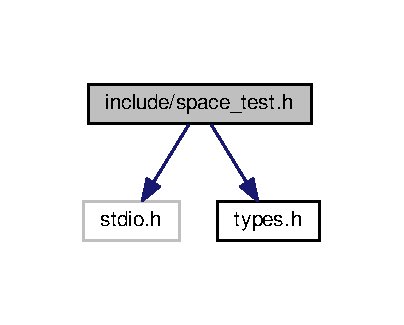
\includegraphics[width=194pt]{space__test_8h__incl}
\end{center}
\end{figure}
This graph shows which files directly or indirectly include this file\+:
\nopagebreak
\begin{figure}[H]
\begin{center}
\leavevmode
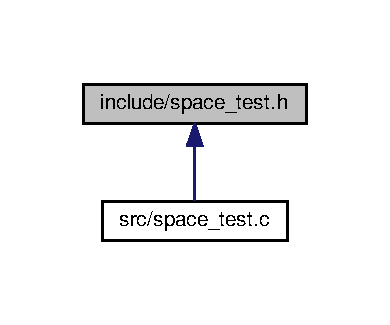
\includegraphics[width=187pt]{space__test_8h__dep__incl}
\end{center}
\end{figure}
\subsection*{Functions}
\begin{DoxyCompactItemize}
\item 
void \hyperlink{space__test_8h_a69278cc022dc5688d4725f8d36317b30}{test1\+\_\+space\+\_\+create} ()
\item 
void \hyperlink{space__test_8h_a012cd3cf37a8d91e2d7098a264c29d65}{test2\+\_\+space\+\_\+create} ()
\item 
void \hyperlink{space__test_8h_af3febdc46ce54799ebfcdbc4330ee93e}{test1\+\_\+space\+\_\+destroy} ()
\item 
void \hyperlink{space__test_8h_ad8a5df09bd9f731be1ce6048e92e58c4}{test2\+\_\+space\+\_\+destroy} ()
\item 
void \hyperlink{space__test_8h_a920df9e02482f4f1e6a5ebcaec523860}{test1\+\_\+space\+\_\+get\+\_\+id} ()
\item 
void \hyperlink{space__test_8h_af9087176b0d3c41d83a17a4918b13e31}{test2\+\_\+space\+\_\+get\+\_\+id} ()
\item 
void \hyperlink{space__test_8h_a07d793d51acfebb4d3261cafbbf35a4b}{test1\+\_\+space\+\_\+get\+\_\+object\+\_\+number} ()
\item 
void \hyperlink{space__test_8h_a77ab44cb3b3511ecdda66c13718d9048}{test2\+\_\+space\+\_\+get\+\_\+object\+\_\+number} ()
\item 
void \hyperlink{space__test_8h_ace18d8edf7b88e4b4d3e84dfa0b244bf}{test3\+\_\+space\+\_\+get\+\_\+object\+\_\+number} ()
\item 
void \hyperlink{space__test_8h_a2569bab6cfeec15f722d232bb8c78c9e}{test1\+\_\+space\+\_\+set\+\_\+name} ()
\item 
void \hyperlink{space__test_8h_a5a868ba017602ba6b58447cb394e81a6}{test2\+\_\+space\+\_\+set\+\_\+name} ()
\item 
void \hyperlink{space__test_8h_aa24a337830006e33706ab6ac1c416b47}{test3\+\_\+space\+\_\+set\+\_\+name} ()
\item 
void \hyperlink{space__test_8h_ad12c42523c517507566c5c68b1527689}{test1\+\_\+space\+\_\+get\+\_\+name} ()
\item 
void \hyperlink{space__test_8h_aee88ed31c63efc674051a4563aed86e2}{test2\+\_\+space\+\_\+get\+\_\+name} ()
\item 
void \hyperlink{space__test_8h_a36f278e9a36d1af63082a6aeb968a094}{test1\+\_\+space\+\_\+set\+\_\+short\+\_\+description} ()
\item 
void \hyperlink{space__test_8h_a1e5f764e51c98d987ceb47df09ed08d7}{test2\+\_\+space\+\_\+set\+\_\+short\+\_\+description} ()
\item 
void \hyperlink{space__test_8h_afe042540e90d5901e352bbd4a45ec4ac}{test3\+\_\+space\+\_\+set\+\_\+short\+\_\+description} ()
\item 
void \hyperlink{space__test_8h_ace49b6853779ebcd4d4d403e73ad6cda}{test1\+\_\+space\+\_\+get\+\_\+short\+\_\+description} ()
\item 
void \hyperlink{space__test_8h_a67b5e5c2289fb036c25e3618e2658954}{test2\+\_\+space\+\_\+get\+\_\+short\+\_\+description} ()
\item 
void \hyperlink{space__test_8h_a5eac430f7edc2c3c762186580bf2f7cb}{test1\+\_\+space\+\_\+set\+\_\+long\+\_\+description} ()
\item 
void \hyperlink{space__test_8h_a669293c8c232547b7bfc913e38856abd}{test2\+\_\+space\+\_\+set\+\_\+long\+\_\+description} ()
\item 
void \hyperlink{space__test_8h_a1273cecbf0126415fa33af5639ee3058}{test3\+\_\+space\+\_\+set\+\_\+long\+\_\+description} ()
\item 
void \hyperlink{space__test_8h_aaec8bbc606d2e3294f4efbe7c102d482}{test1\+\_\+space\+\_\+get\+\_\+long\+\_\+description} ()
\item 
void \hyperlink{space__test_8h_a102af2c9cd571ef59b393a93ecde63aa}{test2\+\_\+space\+\_\+get\+\_\+long\+\_\+description} ()
\item 
void \hyperlink{space__test_8h_a208ae9352ff979024f6ebef4e791356a}{test1\+\_\+space\+\_\+set\+\_\+object} ()
\item 
void \hyperlink{space__test_8h_a6349e2b547c71dee23b96d8bbf7a1806}{test2\+\_\+space\+\_\+set\+\_\+object} ()
\item 
void \hyperlink{space__test_8h_a4a1ca89fa511c04bb07c14edb19c17ba}{test1\+\_\+space\+\_\+get\+\_\+object} ()
\item 
void \hyperlink{space__test_8h_a3d3457a89f705948102cf1e5d4a7b45b}{test1\+\_\+space\+\_\+set\+\_\+north} ()
\item 
void \hyperlink{space__test_8h_a3bc7fe26c1e36ffd195099a9983206e1}{test2\+\_\+space\+\_\+set\+\_\+north} ()
\item 
void \hyperlink{space__test_8h_ac2961dcc4d7645660ca6953a70315b0a}{test3\+\_\+space\+\_\+set\+\_\+north} ()
\item 
void \hyperlink{space__test_8h_a3a87f1e1e173d622bfbd3bcd14e060ca}{test1\+\_\+space\+\_\+get\+\_\+north} ()
\item 
void \hyperlink{space__test_8h_a61891c9cebb9d26dc9f149ad8341517c}{test2\+\_\+space\+\_\+get\+\_\+north} ()
\item 
void \hyperlink{space__test_8h_a21938e16547b3080e9251f960117a859}{test1\+\_\+space\+\_\+set\+\_\+south} ()
\item 
void \hyperlink{space__test_8h_ac9f950741f12ccfcc5ad5d9e71d3d90a}{test2\+\_\+space\+\_\+set\+\_\+south} ()
\item 
void \hyperlink{space__test_8h_ab2626f0045b225c79a8c5d56298e2065}{test3\+\_\+space\+\_\+set\+\_\+south} ()
\item 
void \hyperlink{space__test_8h_a8e345065f58565e131bdb3a9d0096ed5}{test1\+\_\+space\+\_\+get\+\_\+south} ()
\item 
void \hyperlink{space__test_8h_a40fe07c07c1069023b362a9e506c4c59}{test2\+\_\+space\+\_\+get\+\_\+south} ()
\item 
void \hyperlink{space__test_8h_ab1f093af4be3ca8e525d0517cc846f47}{test1\+\_\+space\+\_\+set\+\_\+east} ()
\item 
void \hyperlink{space__test_8h_a5df66d103388be4518c379b224f53770}{test2\+\_\+space\+\_\+set\+\_\+east} ()
\item 
void \hyperlink{space__test_8h_adf98486d8745110660515d14b71b5656}{test3\+\_\+space\+\_\+set\+\_\+east} ()
\item 
void \hyperlink{space__test_8h_a354adb2722b06ec65b7212d2736d6417}{test1\+\_\+space\+\_\+get\+\_\+east} ()
\item 
void \hyperlink{space__test_8h_a249293510e61c6d5465f52c14343d02b}{test2\+\_\+space\+\_\+get\+\_\+east} ()
\item 
void \hyperlink{space__test_8h_ab680a8797f793dffd58546074b87d21f}{test1\+\_\+space\+\_\+set\+\_\+west} ()
\item 
void \hyperlink{space__test_8h_aa51b05ffd99b7bbd8f2dfc23c8f85870}{test2\+\_\+space\+\_\+set\+\_\+west} ()
\item 
void \hyperlink{space__test_8h_a8150758940559ef958649a2fab36bee0}{test3\+\_\+space\+\_\+set\+\_\+west} ()
\item 
void \hyperlink{space__test_8h_a1f08c6866885bfc093717f57b1b86539}{test1\+\_\+space\+\_\+get\+\_\+west} ()
\item 
void \hyperlink{space__test_8h_af1cf02b01c007aec0684186b39666c32}{test2\+\_\+space\+\_\+get\+\_\+west} ()
\item 
void \hyperlink{space__test_8h_a43e340258ebc17b956c845dd0f4d93fa}{test1\+\_\+space\+\_\+get\+\_\+iluminate} ()
\item 
void \hyperlink{space__test_8h_ac3a020093f98ed086245f3f80bd4d415}{test2\+\_\+space\+\_\+get\+\_\+iluminate} ()
\item 
void \hyperlink{space__test_8h_af91f2dc174c3e15c5db66317f1c1a25d}{test1\+\_\+space\+\_\+set\+\_\+iluminate} ()
\item 
void \hyperlink{space__test_8h_a2576a23407d714fa26ce8f988a5df0e5}{test2\+\_\+space\+\_\+set\+\_\+iluminate} ()
\item 
void \hyperlink{space__test_8h_a087e9efe152864bbb919b3d4208f66b7}{test1\+\_\+space\+\_\+set\+\_\+up} ()
\item 
void \hyperlink{space__test_8h_a93508104720cd2f5ba4ac9652d8d238e}{test2\+\_\+space\+\_\+set\+\_\+up} ()
\item 
void \hyperlink{space__test_8h_a4b9cd940aa6ec095996f2051ee938070}{test3\+\_\+space\+\_\+set\+\_\+up} ()
\item 
void \hyperlink{space__test_8h_a27def98869466837b2b9e46c8979b795}{test1\+\_\+space\+\_\+get\+\_\+up} ()
\item 
void \hyperlink{space__test_8h_a293a03e22f1bc96f193cc84abfd23fa4}{test2\+\_\+space\+\_\+get\+\_\+up} ()
\item 
void \hyperlink{space__test_8h_acfdc180b8543b1fd7e320423416a7eec}{test1\+\_\+space\+\_\+set\+\_\+down} ()
\item 
void \hyperlink{space__test_8h_a4d579ee19e22dfc43891f0dca5db14a6}{test2\+\_\+space\+\_\+set\+\_\+down} ()
\item 
void \hyperlink{space__test_8h_a38591396f4d83f2f2783de8944fe93eb}{test3\+\_\+space\+\_\+set\+\_\+down} ()
\item 
void \hyperlink{space__test_8h_a31b56fea7bd46484d0e2e21dda7add5d}{test1\+\_\+space\+\_\+get\+\_\+down} ()
\item 
void \hyperlink{space__test_8h_a4390a534575e1516d30140e8e40e3b52}{test2\+\_\+space\+\_\+get\+\_\+down} ()
\end{DoxyCompactItemize}


\subsection{Detailed Description}
It declares the tests for the space module. 

\begin{DoxyAuthor}{Author}
Juan Moreno 
\end{DoxyAuthor}
\begin{DoxyVersion}{Version}
2.\+0 
\end{DoxyVersion}
\begin{DoxyDate}{Date}
01-\/04-\/2018 
\end{DoxyDate}


\subsection{Function Documentation}
\index{space\+\_\+test.\+h@{space\+\_\+test.\+h}!test1\+\_\+space\+\_\+create@{test1\+\_\+space\+\_\+create}}
\index{test1\+\_\+space\+\_\+create@{test1\+\_\+space\+\_\+create}!space\+\_\+test.\+h@{space\+\_\+test.\+h}}
\subsubsection[{\texorpdfstring{test1\+\_\+space\+\_\+create()}{test1_space_create()}}]{\setlength{\rightskip}{0pt plus 5cm}void test1\+\_\+space\+\_\+create (
\begin{DoxyParamCaption}
{}
\end{DoxyParamCaption}
)}\hypertarget{space__test_8h_a69278cc022dc5688d4725f8d36317b30}{}\label{space__test_8h_a69278cc022dc5688d4725f8d36317b30}
\begin{DoxyRefDesc}{Test}
\item[\hyperlink{test__test000121}{Test}]Test space creation \end{DoxyRefDesc}
\begin{DoxyPrecond}{Precondition}
Space ID 
\end{DoxyPrecond}
\begin{DoxyPostcond}{Postcondition}
Non N\+U\+LL pointer to space 
\end{DoxyPostcond}
\index{space\+\_\+test.\+h@{space\+\_\+test.\+h}!test1\+\_\+space\+\_\+destroy@{test1\+\_\+space\+\_\+destroy}}
\index{test1\+\_\+space\+\_\+destroy@{test1\+\_\+space\+\_\+destroy}!space\+\_\+test.\+h@{space\+\_\+test.\+h}}
\subsubsection[{\texorpdfstring{test1\+\_\+space\+\_\+destroy()}{test1_space_destroy()}}]{\setlength{\rightskip}{0pt plus 5cm}void test1\+\_\+space\+\_\+destroy (
\begin{DoxyParamCaption}
{}
\end{DoxyParamCaption}
)}\hypertarget{space__test_8h_af3febdc46ce54799ebfcdbc4330ee93e}{}\label{space__test_8h_af3febdc46ce54799ebfcdbc4330ee93e}
\begin{DoxyRefDesc}{Test}
\item[\hyperlink{test__test000123}{Test}]Test space destruction \end{DoxyRefDesc}
\begin{DoxyPrecond}{Precondition}
N\+U\+LL pointer to space 
\end{DoxyPrecond}
\begin{DoxyPostcond}{Postcondition}
S\+T\+A\+T\+US==E\+R\+R\+OR 
\end{DoxyPostcond}
\index{space\+\_\+test.\+h@{space\+\_\+test.\+h}!test1\+\_\+space\+\_\+get\+\_\+down@{test1\+\_\+space\+\_\+get\+\_\+down}}
\index{test1\+\_\+space\+\_\+get\+\_\+down@{test1\+\_\+space\+\_\+get\+\_\+down}!space\+\_\+test.\+h@{space\+\_\+test.\+h}}
\subsubsection[{\texorpdfstring{test1\+\_\+space\+\_\+get\+\_\+down()}{test1_space_get_down()}}]{\setlength{\rightskip}{0pt plus 5cm}void test1\+\_\+space\+\_\+get\+\_\+down (
\begin{DoxyParamCaption}
{}
\end{DoxyParamCaption}
)}\hypertarget{space__test_8h_a31b56fea7bd46484d0e2e21dda7add5d}{}\label{space__test_8h_a31b56fea7bd46484d0e2e21dda7add5d}
\begin{DoxyRefDesc}{Test}
\item[\hyperlink{test__test000180}{Test}]Test function for getting down space \end{DoxyRefDesc}
\begin{DoxyPrecond}{Precondition}
Space pointer N\+U\+LL 
\end{DoxyPrecond}
\begin{DoxyPostcond}{Postcondition}
N\+O\+\_\+\+ID 
\end{DoxyPostcond}
\index{space\+\_\+test.\+h@{space\+\_\+test.\+h}!test1\+\_\+space\+\_\+get\+\_\+east@{test1\+\_\+space\+\_\+get\+\_\+east}}
\index{test1\+\_\+space\+\_\+get\+\_\+east@{test1\+\_\+space\+\_\+get\+\_\+east}!space\+\_\+test.\+h@{space\+\_\+test.\+h}}
\subsubsection[{\texorpdfstring{test1\+\_\+space\+\_\+get\+\_\+east()}{test1_space_get_east()}}]{\setlength{\rightskip}{0pt plus 5cm}void test1\+\_\+space\+\_\+get\+\_\+east (
\begin{DoxyParamCaption}
{}
\end{DoxyParamCaption}
)}\hypertarget{space__test_8h_a354adb2722b06ec65b7212d2736d6417}{}\label{space__test_8h_a354adb2722b06ec65b7212d2736d6417}
\begin{DoxyRefDesc}{Test}
\item[\hyperlink{test__test000161}{Test}]Test function for getting east space \end{DoxyRefDesc}
\begin{DoxyPrecond}{Precondition}
Space pointer N\+U\+LL 
\end{DoxyPrecond}
\begin{DoxyPostcond}{Postcondition}
N\+O\+\_\+\+ID 
\end{DoxyPostcond}
\index{space\+\_\+test.\+h@{space\+\_\+test.\+h}!test1\+\_\+space\+\_\+get\+\_\+id@{test1\+\_\+space\+\_\+get\+\_\+id}}
\index{test1\+\_\+space\+\_\+get\+\_\+id@{test1\+\_\+space\+\_\+get\+\_\+id}!space\+\_\+test.\+h@{space\+\_\+test.\+h}}
\subsubsection[{\texorpdfstring{test1\+\_\+space\+\_\+get\+\_\+id()}{test1_space_get_id()}}]{\setlength{\rightskip}{0pt plus 5cm}void test1\+\_\+space\+\_\+get\+\_\+id (
\begin{DoxyParamCaption}
{}
\end{DoxyParamCaption}
)}\hypertarget{space__test_8h_a920df9e02482f4f1e6a5ebcaec523860}{}\label{space__test_8h_a920df9e02482f4f1e6a5ebcaec523860}
\begin{DoxyRefDesc}{Test}
\item[\hyperlink{test__test000125}{Test}]Test id of space \end{DoxyRefDesc}
\begin{DoxyPrecond}{Precondition}
Space pointer N\+U\+LL 
\end{DoxyPrecond}
\begin{DoxyPostcond}{Postcondition}
N\+O\+\_\+\+ID 
\end{DoxyPostcond}
\index{space\+\_\+test.\+h@{space\+\_\+test.\+h}!test1\+\_\+space\+\_\+get\+\_\+iluminate@{test1\+\_\+space\+\_\+get\+\_\+iluminate}}
\index{test1\+\_\+space\+\_\+get\+\_\+iluminate@{test1\+\_\+space\+\_\+get\+\_\+iluminate}!space\+\_\+test.\+h@{space\+\_\+test.\+h}}
\subsubsection[{\texorpdfstring{test1\+\_\+space\+\_\+get\+\_\+iluminate()}{test1_space_get_iluminate()}}]{\setlength{\rightskip}{0pt plus 5cm}void test1\+\_\+space\+\_\+get\+\_\+iluminate (
\begin{DoxyParamCaption}
{}
\end{DoxyParamCaption}
)}\hypertarget{space__test_8h_a43e340258ebc17b956c845dd0f4d93fa}{}\label{space__test_8h_a43e340258ebc17b956c845dd0f4d93fa}
\begin{DoxyRefDesc}{Test}
\item[\hyperlink{test__test000168}{Test}]Test function for getting iluminate property of space \end{DoxyRefDesc}
\begin{DoxyPrecond}{Precondition}
Space pointer 
\end{DoxyPrecond}
\begin{DoxyPostcond}{Postcondition}
F\+A\+L\+SE 
\end{DoxyPostcond}
\index{space\+\_\+test.\+h@{space\+\_\+test.\+h}!test1\+\_\+space\+\_\+get\+\_\+long\+\_\+description@{test1\+\_\+space\+\_\+get\+\_\+long\+\_\+description}}
\index{test1\+\_\+space\+\_\+get\+\_\+long\+\_\+description@{test1\+\_\+space\+\_\+get\+\_\+long\+\_\+description}!space\+\_\+test.\+h@{space\+\_\+test.\+h}}
\subsubsection[{\texorpdfstring{test1\+\_\+space\+\_\+get\+\_\+long\+\_\+description()}{test1_space_get_long_description()}}]{\setlength{\rightskip}{0pt plus 5cm}void test1\+\_\+space\+\_\+get\+\_\+long\+\_\+description (
\begin{DoxyParamCaption}
{}
\end{DoxyParamCaption}
)}\hypertarget{space__test_8h_aaec8bbc606d2e3294f4efbe7c102d482}{}\label{space__test_8h_aaec8bbc606d2e3294f4efbe7c102d482}
\begin{DoxyRefDesc}{Test}
\item[\hyperlink{test__test000143}{Test}]Test function for description of space obtaining \end{DoxyRefDesc}
\begin{DoxyPrecond}{Precondition}
Space pointer 
\end{DoxyPrecond}
\begin{DoxyPostcond}{Postcondition}
String with name 
\end{DoxyPostcond}
\index{space\+\_\+test.\+h@{space\+\_\+test.\+h}!test1\+\_\+space\+\_\+get\+\_\+name@{test1\+\_\+space\+\_\+get\+\_\+name}}
\index{test1\+\_\+space\+\_\+get\+\_\+name@{test1\+\_\+space\+\_\+get\+\_\+name}!space\+\_\+test.\+h@{space\+\_\+test.\+h}}
\subsubsection[{\texorpdfstring{test1\+\_\+space\+\_\+get\+\_\+name()}{test1_space_get_name()}}]{\setlength{\rightskip}{0pt plus 5cm}void test1\+\_\+space\+\_\+get\+\_\+name (
\begin{DoxyParamCaption}
{}
\end{DoxyParamCaption}
)}\hypertarget{space__test_8h_ad12c42523c517507566c5c68b1527689}{}\label{space__test_8h_ad12c42523c517507566c5c68b1527689}
\begin{DoxyRefDesc}{Test}
\item[\hyperlink{test__test000133}{Test}]Test function for space\+\_\+name obtaining \end{DoxyRefDesc}
\begin{DoxyPrecond}{Precondition}
Space pointer 
\end{DoxyPrecond}
\begin{DoxyPostcond}{Postcondition}
String with name 
\end{DoxyPostcond}
\index{space\+\_\+test.\+h@{space\+\_\+test.\+h}!test1\+\_\+space\+\_\+get\+\_\+north@{test1\+\_\+space\+\_\+get\+\_\+north}}
\index{test1\+\_\+space\+\_\+get\+\_\+north@{test1\+\_\+space\+\_\+get\+\_\+north}!space\+\_\+test.\+h@{space\+\_\+test.\+h}}
\subsubsection[{\texorpdfstring{test1\+\_\+space\+\_\+get\+\_\+north()}{test1_space_get_north()}}]{\setlength{\rightskip}{0pt plus 5cm}void test1\+\_\+space\+\_\+get\+\_\+north (
\begin{DoxyParamCaption}
{}
\end{DoxyParamCaption}
)}\hypertarget{space__test_8h_a3a87f1e1e173d622bfbd3bcd14e060ca}{}\label{space__test_8h_a3a87f1e1e173d622bfbd3bcd14e060ca}
\begin{DoxyRefDesc}{Test}
\item[\hyperlink{test__test000151}{Test}]Test function for getting north space \end{DoxyRefDesc}
\begin{DoxyPrecond}{Precondition}
Space pointer N\+U\+LL 
\end{DoxyPrecond}
\begin{DoxyPostcond}{Postcondition}
N\+O\+\_\+\+ID 
\end{DoxyPostcond}
\index{space\+\_\+test.\+h@{space\+\_\+test.\+h}!test1\+\_\+space\+\_\+get\+\_\+object@{test1\+\_\+space\+\_\+get\+\_\+object}}
\index{test1\+\_\+space\+\_\+get\+\_\+object@{test1\+\_\+space\+\_\+get\+\_\+object}!space\+\_\+test.\+h@{space\+\_\+test.\+h}}
\subsubsection[{\texorpdfstring{test1\+\_\+space\+\_\+get\+\_\+object()}{test1_space_get_object()}}]{\setlength{\rightskip}{0pt plus 5cm}void test1\+\_\+space\+\_\+get\+\_\+object (
\begin{DoxyParamCaption}
{}
\end{DoxyParamCaption}
)}\hypertarget{space__test_8h_a4a1ca89fa511c04bb07c14edb19c17ba}{}\label{space__test_8h_a4a1ca89fa511c04bb07c14edb19c17ba}
\begin{DoxyRefDesc}{Test}
\item[\hyperlink{test__test000147}{Test}]Test function for getting objects \end{DoxyRefDesc}
\begin{DoxyPrecond}{Precondition}
Space pointer and object pointer 
\end{DoxyPrecond}
\begin{DoxyPostcond}{Postcondition}
Not N\+U\+LL 
\end{DoxyPostcond}
\index{space\+\_\+test.\+h@{space\+\_\+test.\+h}!test1\+\_\+space\+\_\+get\+\_\+object\+\_\+number@{test1\+\_\+space\+\_\+get\+\_\+object\+\_\+number}}
\index{test1\+\_\+space\+\_\+get\+\_\+object\+\_\+number@{test1\+\_\+space\+\_\+get\+\_\+object\+\_\+number}!space\+\_\+test.\+h@{space\+\_\+test.\+h}}
\subsubsection[{\texorpdfstring{test1\+\_\+space\+\_\+get\+\_\+object\+\_\+number()}{test1_space_get_object_number()}}]{\setlength{\rightskip}{0pt plus 5cm}void test1\+\_\+space\+\_\+get\+\_\+object\+\_\+number (
\begin{DoxyParamCaption}
{}
\end{DoxyParamCaption}
)}\hypertarget{space__test_8h_a07d793d51acfebb4d3261cafbbf35a4b}{}\label{space__test_8h_a07d793d51acfebb4d3261cafbbf35a4b}
\begin{DoxyRefDesc}{Test}
\item[\hyperlink{test__test000127}{Test}]Test number of objects in space \end{DoxyRefDesc}
\begin{DoxyPrecond}{Precondition}
Space pointer N\+U\+LL 
\end{DoxyPrecond}
\begin{DoxyPostcond}{Postcondition}
N\+O\+\_\+\+ID 
\end{DoxyPostcond}
\index{space\+\_\+test.\+h@{space\+\_\+test.\+h}!test1\+\_\+space\+\_\+get\+\_\+short\+\_\+description@{test1\+\_\+space\+\_\+get\+\_\+short\+\_\+description}}
\index{test1\+\_\+space\+\_\+get\+\_\+short\+\_\+description@{test1\+\_\+space\+\_\+get\+\_\+short\+\_\+description}!space\+\_\+test.\+h@{space\+\_\+test.\+h}}
\subsubsection[{\texorpdfstring{test1\+\_\+space\+\_\+get\+\_\+short\+\_\+description()}{test1_space_get_short_description()}}]{\setlength{\rightskip}{0pt plus 5cm}void test1\+\_\+space\+\_\+get\+\_\+short\+\_\+description (
\begin{DoxyParamCaption}
{}
\end{DoxyParamCaption}
)}\hypertarget{space__test_8h_ace49b6853779ebcd4d4d403e73ad6cda}{}\label{space__test_8h_ace49b6853779ebcd4d4d403e73ad6cda}
\begin{DoxyRefDesc}{Test}
\item[\hyperlink{test__test000138}{Test}]Test function for description of space obtaining \end{DoxyRefDesc}
\begin{DoxyPrecond}{Precondition}
Space pointer 
\end{DoxyPrecond}
\begin{DoxyPostcond}{Postcondition}
String with name 
\end{DoxyPostcond}
\index{space\+\_\+test.\+h@{space\+\_\+test.\+h}!test1\+\_\+space\+\_\+get\+\_\+south@{test1\+\_\+space\+\_\+get\+\_\+south}}
\index{test1\+\_\+space\+\_\+get\+\_\+south@{test1\+\_\+space\+\_\+get\+\_\+south}!space\+\_\+test.\+h@{space\+\_\+test.\+h}}
\subsubsection[{\texorpdfstring{test1\+\_\+space\+\_\+get\+\_\+south()}{test1_space_get_south()}}]{\setlength{\rightskip}{0pt plus 5cm}void test1\+\_\+space\+\_\+get\+\_\+south (
\begin{DoxyParamCaption}
{}
\end{DoxyParamCaption}
)}\hypertarget{space__test_8h_a8e345065f58565e131bdb3a9d0096ed5}{}\label{space__test_8h_a8e345065f58565e131bdb3a9d0096ed5}
\begin{DoxyRefDesc}{Test}
\item[\hyperlink{test__test000156}{Test}]Test function for getting south space \end{DoxyRefDesc}
\begin{DoxyPrecond}{Precondition}
Space pointer N\+U\+LL 
\end{DoxyPrecond}
\begin{DoxyPostcond}{Postcondition}
N\+O\+\_\+\+ID 
\end{DoxyPostcond}
\index{space\+\_\+test.\+h@{space\+\_\+test.\+h}!test1\+\_\+space\+\_\+get\+\_\+up@{test1\+\_\+space\+\_\+get\+\_\+up}}
\index{test1\+\_\+space\+\_\+get\+\_\+up@{test1\+\_\+space\+\_\+get\+\_\+up}!space\+\_\+test.\+h@{space\+\_\+test.\+h}}
\subsubsection[{\texorpdfstring{test1\+\_\+space\+\_\+get\+\_\+up()}{test1_space_get_up()}}]{\setlength{\rightskip}{0pt plus 5cm}void test1\+\_\+space\+\_\+get\+\_\+up (
\begin{DoxyParamCaption}
{}
\end{DoxyParamCaption}
)}\hypertarget{space__test_8h_a27def98869466837b2b9e46c8979b795}{}\label{space__test_8h_a27def98869466837b2b9e46c8979b795}
\begin{DoxyRefDesc}{Test}
\item[\hyperlink{test__test000175}{Test}]Test function for getting up space \end{DoxyRefDesc}
\begin{DoxyPrecond}{Precondition}
Space pointer N\+U\+LL 
\end{DoxyPrecond}
\begin{DoxyPostcond}{Postcondition}
N\+O\+\_\+\+ID 
\end{DoxyPostcond}
\index{space\+\_\+test.\+h@{space\+\_\+test.\+h}!test1\+\_\+space\+\_\+get\+\_\+west@{test1\+\_\+space\+\_\+get\+\_\+west}}
\index{test1\+\_\+space\+\_\+get\+\_\+west@{test1\+\_\+space\+\_\+get\+\_\+west}!space\+\_\+test.\+h@{space\+\_\+test.\+h}}
\subsubsection[{\texorpdfstring{test1\+\_\+space\+\_\+get\+\_\+west()}{test1_space_get_west()}}]{\setlength{\rightskip}{0pt plus 5cm}void test1\+\_\+space\+\_\+get\+\_\+west (
\begin{DoxyParamCaption}
{}
\end{DoxyParamCaption}
)}\hypertarget{space__test_8h_a1f08c6866885bfc093717f57b1b86539}{}\label{space__test_8h_a1f08c6866885bfc093717f57b1b86539}
\begin{DoxyRefDesc}{Test}
\item[\hyperlink{test__test000166}{Test}]Test function for getting west space \end{DoxyRefDesc}
\begin{DoxyPrecond}{Precondition}
Space pointer N\+U\+LL 
\end{DoxyPrecond}
\begin{DoxyPostcond}{Postcondition}
N\+O\+\_\+\+ID 
\end{DoxyPostcond}
\index{space\+\_\+test.\+h@{space\+\_\+test.\+h}!test1\+\_\+space\+\_\+set\+\_\+down@{test1\+\_\+space\+\_\+set\+\_\+down}}
\index{test1\+\_\+space\+\_\+set\+\_\+down@{test1\+\_\+space\+\_\+set\+\_\+down}!space\+\_\+test.\+h@{space\+\_\+test.\+h}}
\subsubsection[{\texorpdfstring{test1\+\_\+space\+\_\+set\+\_\+down()}{test1_space_set_down()}}]{\setlength{\rightskip}{0pt plus 5cm}void test1\+\_\+space\+\_\+set\+\_\+down (
\begin{DoxyParamCaption}
{}
\end{DoxyParamCaption}
)}\hypertarget{space__test_8h_acfdc180b8543b1fd7e320423416a7eec}{}\label{space__test_8h_acfdc180b8543b1fd7e320423416a7eec}
\begin{DoxyRefDesc}{Test}
\item[\hyperlink{test__test000177}{Test}]Test function for setting down space \end{DoxyRefDesc}
\begin{DoxyPrecond}{Precondition}
Space pointer N\+U\+LL 
\end{DoxyPrecond}
\begin{DoxyPostcond}{Postcondition}
E\+R\+R\+OR 
\end{DoxyPostcond}
\index{space\+\_\+test.\+h@{space\+\_\+test.\+h}!test1\+\_\+space\+\_\+set\+\_\+east@{test1\+\_\+space\+\_\+set\+\_\+east}}
\index{test1\+\_\+space\+\_\+set\+\_\+east@{test1\+\_\+space\+\_\+set\+\_\+east}!space\+\_\+test.\+h@{space\+\_\+test.\+h}}
\subsubsection[{\texorpdfstring{test1\+\_\+space\+\_\+set\+\_\+east()}{test1_space_set_east()}}]{\setlength{\rightskip}{0pt plus 5cm}void test1\+\_\+space\+\_\+set\+\_\+east (
\begin{DoxyParamCaption}
{}
\end{DoxyParamCaption}
)}\hypertarget{space__test_8h_ab1f093af4be3ca8e525d0517cc846f47}{}\label{space__test_8h_ab1f093af4be3ca8e525d0517cc846f47}
\begin{DoxyRefDesc}{Test}
\item[\hyperlink{test__test000158}{Test}]Test function for setting east space \end{DoxyRefDesc}
\begin{DoxyPrecond}{Precondition}
Space pointer N\+U\+LL 
\end{DoxyPrecond}
\begin{DoxyPostcond}{Postcondition}
E\+R\+R\+OR 
\end{DoxyPostcond}
\index{space\+\_\+test.\+h@{space\+\_\+test.\+h}!test1\+\_\+space\+\_\+set\+\_\+iluminate@{test1\+\_\+space\+\_\+set\+\_\+iluminate}}
\index{test1\+\_\+space\+\_\+set\+\_\+iluminate@{test1\+\_\+space\+\_\+set\+\_\+iluminate}!space\+\_\+test.\+h@{space\+\_\+test.\+h}}
\subsubsection[{\texorpdfstring{test1\+\_\+space\+\_\+set\+\_\+iluminate()}{test1_space_set_iluminate()}}]{\setlength{\rightskip}{0pt plus 5cm}void test1\+\_\+space\+\_\+set\+\_\+iluminate (
\begin{DoxyParamCaption}
{}
\end{DoxyParamCaption}
)}\hypertarget{space__test_8h_af91f2dc174c3e15c5db66317f1c1a25d}{}\label{space__test_8h_af91f2dc174c3e15c5db66317f1c1a25d}
\begin{DoxyRefDesc}{Test}
\item[\hyperlink{test__test000170}{Test}]Test function for setting iluminate property of space \end{DoxyRefDesc}
\begin{DoxyPrecond}{Precondition}
Space pointer and F\+A\+L\+SE 
\end{DoxyPrecond}
\begin{DoxyPostcond}{Postcondition}
F\+A\+L\+SE 
\end{DoxyPostcond}
\index{space\+\_\+test.\+h@{space\+\_\+test.\+h}!test1\+\_\+space\+\_\+set\+\_\+long\+\_\+description@{test1\+\_\+space\+\_\+set\+\_\+long\+\_\+description}}
\index{test1\+\_\+space\+\_\+set\+\_\+long\+\_\+description@{test1\+\_\+space\+\_\+set\+\_\+long\+\_\+description}!space\+\_\+test.\+h@{space\+\_\+test.\+h}}
\subsubsection[{\texorpdfstring{test1\+\_\+space\+\_\+set\+\_\+long\+\_\+description()}{test1_space_set_long_description()}}]{\setlength{\rightskip}{0pt plus 5cm}void test1\+\_\+space\+\_\+set\+\_\+long\+\_\+description (
\begin{DoxyParamCaption}
{}
\end{DoxyParamCaption}
)}\hypertarget{space__test_8h_a5eac430f7edc2c3c762186580bf2f7cb}{}\label{space__test_8h_a5eac430f7edc2c3c762186580bf2f7cb}
\begin{DoxyRefDesc}{Test}
\item[\hyperlink{test__test000140}{Test}]Test function for description of space setting \end{DoxyRefDesc}
\begin{DoxyPrecond}{Precondition}
String of characters 
\end{DoxyPrecond}
\begin{DoxyPostcond}{Postcondition}
S\+T\+A\+T\+US=OK 
\end{DoxyPostcond}
\index{space\+\_\+test.\+h@{space\+\_\+test.\+h}!test1\+\_\+space\+\_\+set\+\_\+name@{test1\+\_\+space\+\_\+set\+\_\+name}}
\index{test1\+\_\+space\+\_\+set\+\_\+name@{test1\+\_\+space\+\_\+set\+\_\+name}!space\+\_\+test.\+h@{space\+\_\+test.\+h}}
\subsubsection[{\texorpdfstring{test1\+\_\+space\+\_\+set\+\_\+name()}{test1_space_set_name()}}]{\setlength{\rightskip}{0pt plus 5cm}void test1\+\_\+space\+\_\+set\+\_\+name (
\begin{DoxyParamCaption}
{}
\end{DoxyParamCaption}
)}\hypertarget{space__test_8h_a2569bab6cfeec15f722d232bb8c78c9e}{}\label{space__test_8h_a2569bab6cfeec15f722d232bb8c78c9e}
\begin{DoxyRefDesc}{Test}
\item[\hyperlink{test__test000130}{Test}]Test function for space\+\_\+name setting \end{DoxyRefDesc}
\begin{DoxyPrecond}{Precondition}
String with space name 
\end{DoxyPrecond}
\begin{DoxyPostcond}{Postcondition}
Ouput==OK 
\end{DoxyPostcond}
\index{space\+\_\+test.\+h@{space\+\_\+test.\+h}!test1\+\_\+space\+\_\+set\+\_\+north@{test1\+\_\+space\+\_\+set\+\_\+north}}
\index{test1\+\_\+space\+\_\+set\+\_\+north@{test1\+\_\+space\+\_\+set\+\_\+north}!space\+\_\+test.\+h@{space\+\_\+test.\+h}}
\subsubsection[{\texorpdfstring{test1\+\_\+space\+\_\+set\+\_\+north()}{test1_space_set_north()}}]{\setlength{\rightskip}{0pt plus 5cm}void test1\+\_\+space\+\_\+set\+\_\+north (
\begin{DoxyParamCaption}
{}
\end{DoxyParamCaption}
)}\hypertarget{space__test_8h_a3d3457a89f705948102cf1e5d4a7b45b}{}\label{space__test_8h_a3d3457a89f705948102cf1e5d4a7b45b}
\begin{DoxyRefDesc}{Test}
\item[\hyperlink{test__test000148}{Test}]Test function for setting north space \end{DoxyRefDesc}
\begin{DoxyPrecond}{Precondition}
Space pointer N\+U\+LL 
\end{DoxyPrecond}
\begin{DoxyPostcond}{Postcondition}
E\+R\+R\+OR 
\end{DoxyPostcond}
\index{space\+\_\+test.\+h@{space\+\_\+test.\+h}!test1\+\_\+space\+\_\+set\+\_\+object@{test1\+\_\+space\+\_\+set\+\_\+object}}
\index{test1\+\_\+space\+\_\+set\+\_\+object@{test1\+\_\+space\+\_\+set\+\_\+object}!space\+\_\+test.\+h@{space\+\_\+test.\+h}}
\subsubsection[{\texorpdfstring{test1\+\_\+space\+\_\+set\+\_\+object()}{test1_space_set_object()}}]{\setlength{\rightskip}{0pt plus 5cm}void test1\+\_\+space\+\_\+set\+\_\+object (
\begin{DoxyParamCaption}
{}
\end{DoxyParamCaption}
)}\hypertarget{space__test_8h_a208ae9352ff979024f6ebef4e791356a}{}\label{space__test_8h_a208ae9352ff979024f6ebef4e791356a}
\begin{DoxyRefDesc}{Test}
\item[\hyperlink{test__test000145}{Test}]Test function for setting objects \end{DoxyRefDesc}
\begin{DoxyPrecond}{Precondition}
Space pointer N\+U\+LL and object pointer 
\end{DoxyPrecond}
\begin{DoxyPostcond}{Postcondition}
E\+R\+R\+OR 
\end{DoxyPostcond}
\index{space\+\_\+test.\+h@{space\+\_\+test.\+h}!test1\+\_\+space\+\_\+set\+\_\+short\+\_\+description@{test1\+\_\+space\+\_\+set\+\_\+short\+\_\+description}}
\index{test1\+\_\+space\+\_\+set\+\_\+short\+\_\+description@{test1\+\_\+space\+\_\+set\+\_\+short\+\_\+description}!space\+\_\+test.\+h@{space\+\_\+test.\+h}}
\subsubsection[{\texorpdfstring{test1\+\_\+space\+\_\+set\+\_\+short\+\_\+description()}{test1_space_set_short_description()}}]{\setlength{\rightskip}{0pt plus 5cm}void test1\+\_\+space\+\_\+set\+\_\+short\+\_\+description (
\begin{DoxyParamCaption}
{}
\end{DoxyParamCaption}
)}\hypertarget{space__test_8h_a36f278e9a36d1af63082a6aeb968a094}{}\label{space__test_8h_a36f278e9a36d1af63082a6aeb968a094}
\begin{DoxyRefDesc}{Test}
\item[\hyperlink{test__test000135}{Test}]Test function for description of space setting \end{DoxyRefDesc}
\begin{DoxyPrecond}{Precondition}
String of characters 
\end{DoxyPrecond}
\begin{DoxyPostcond}{Postcondition}
S\+T\+A\+T\+US=OK 
\end{DoxyPostcond}
\index{space\+\_\+test.\+h@{space\+\_\+test.\+h}!test1\+\_\+space\+\_\+set\+\_\+south@{test1\+\_\+space\+\_\+set\+\_\+south}}
\index{test1\+\_\+space\+\_\+set\+\_\+south@{test1\+\_\+space\+\_\+set\+\_\+south}!space\+\_\+test.\+h@{space\+\_\+test.\+h}}
\subsubsection[{\texorpdfstring{test1\+\_\+space\+\_\+set\+\_\+south()}{test1_space_set_south()}}]{\setlength{\rightskip}{0pt plus 5cm}void test1\+\_\+space\+\_\+set\+\_\+south (
\begin{DoxyParamCaption}
{}
\end{DoxyParamCaption}
)}\hypertarget{space__test_8h_a21938e16547b3080e9251f960117a859}{}\label{space__test_8h_a21938e16547b3080e9251f960117a859}
\begin{DoxyRefDesc}{Test}
\item[\hyperlink{test__test000153}{Test}]Test function for setting south space \end{DoxyRefDesc}
\begin{DoxyPrecond}{Precondition}
Space pointer N\+U\+LL 
\end{DoxyPrecond}
\begin{DoxyPostcond}{Postcondition}
E\+R\+R\+OR 
\end{DoxyPostcond}
\index{space\+\_\+test.\+h@{space\+\_\+test.\+h}!test1\+\_\+space\+\_\+set\+\_\+up@{test1\+\_\+space\+\_\+set\+\_\+up}}
\index{test1\+\_\+space\+\_\+set\+\_\+up@{test1\+\_\+space\+\_\+set\+\_\+up}!space\+\_\+test.\+h@{space\+\_\+test.\+h}}
\subsubsection[{\texorpdfstring{test1\+\_\+space\+\_\+set\+\_\+up()}{test1_space_set_up()}}]{\setlength{\rightskip}{0pt plus 5cm}void test1\+\_\+space\+\_\+set\+\_\+up (
\begin{DoxyParamCaption}
{}
\end{DoxyParamCaption}
)}\hypertarget{space__test_8h_a087e9efe152864bbb919b3d4208f66b7}{}\label{space__test_8h_a087e9efe152864bbb919b3d4208f66b7}
\begin{DoxyRefDesc}{Test}
\item[\hyperlink{test__test000172}{Test}]Test function for setting up space \end{DoxyRefDesc}
\begin{DoxyPrecond}{Precondition}
Space pointer N\+U\+LL 
\end{DoxyPrecond}
\begin{DoxyPostcond}{Postcondition}
E\+R\+R\+OR 
\end{DoxyPostcond}
\index{space\+\_\+test.\+h@{space\+\_\+test.\+h}!test1\+\_\+space\+\_\+set\+\_\+west@{test1\+\_\+space\+\_\+set\+\_\+west}}
\index{test1\+\_\+space\+\_\+set\+\_\+west@{test1\+\_\+space\+\_\+set\+\_\+west}!space\+\_\+test.\+h@{space\+\_\+test.\+h}}
\subsubsection[{\texorpdfstring{test1\+\_\+space\+\_\+set\+\_\+west()}{test1_space_set_west()}}]{\setlength{\rightskip}{0pt plus 5cm}void test1\+\_\+space\+\_\+set\+\_\+west (
\begin{DoxyParamCaption}
{}
\end{DoxyParamCaption}
)}\hypertarget{space__test_8h_ab680a8797f793dffd58546074b87d21f}{}\label{space__test_8h_ab680a8797f793dffd58546074b87d21f}
\begin{DoxyRefDesc}{Test}
\item[\hyperlink{test__test000163}{Test}]Test function for setting west space \end{DoxyRefDesc}
\begin{DoxyPrecond}{Precondition}
Space pointer N\+U\+LL 
\end{DoxyPrecond}
\begin{DoxyPostcond}{Postcondition}
E\+R\+R\+OR 
\end{DoxyPostcond}
\index{space\+\_\+test.\+h@{space\+\_\+test.\+h}!test2\+\_\+space\+\_\+create@{test2\+\_\+space\+\_\+create}}
\index{test2\+\_\+space\+\_\+create@{test2\+\_\+space\+\_\+create}!space\+\_\+test.\+h@{space\+\_\+test.\+h}}
\subsubsection[{\texorpdfstring{test2\+\_\+space\+\_\+create()}{test2_space_create()}}]{\setlength{\rightskip}{0pt plus 5cm}void test2\+\_\+space\+\_\+create (
\begin{DoxyParamCaption}
{}
\end{DoxyParamCaption}
)}\hypertarget{space__test_8h_a012cd3cf37a8d91e2d7098a264c29d65}{}\label{space__test_8h_a012cd3cf37a8d91e2d7098a264c29d65}
\begin{DoxyRefDesc}{Test}
\item[\hyperlink{test__test000122}{Test}]Test space creation \end{DoxyRefDesc}
\begin{DoxyPrecond}{Precondition}
Space ID 
\end{DoxyPrecond}
\begin{DoxyPostcond}{Postcondition}
Space\+\_\+\+ID == Supplied Space Id 
\end{DoxyPostcond}
\index{space\+\_\+test.\+h@{space\+\_\+test.\+h}!test2\+\_\+space\+\_\+destroy@{test2\+\_\+space\+\_\+destroy}}
\index{test2\+\_\+space\+\_\+destroy@{test2\+\_\+space\+\_\+destroy}!space\+\_\+test.\+h@{space\+\_\+test.\+h}}
\subsubsection[{\texorpdfstring{test2\+\_\+space\+\_\+destroy()}{test2_space_destroy()}}]{\setlength{\rightskip}{0pt plus 5cm}void test2\+\_\+space\+\_\+destroy (
\begin{DoxyParamCaption}
{}
\end{DoxyParamCaption}
)}\hypertarget{space__test_8h_ad8a5df09bd9f731be1ce6048e92e58c4}{}\label{space__test_8h_ad8a5df09bd9f731be1ce6048e92e58c4}
\begin{DoxyRefDesc}{Test}
\item[\hyperlink{test__test000124}{Test}]Test space destruction \end{DoxyRefDesc}
\begin{DoxyPrecond}{Precondition}
Space pointer 
\end{DoxyPrecond}
\begin{DoxyPostcond}{Postcondition}
S\+T\+A\+T\+US==OK 
\end{DoxyPostcond}
\index{space\+\_\+test.\+h@{space\+\_\+test.\+h}!test2\+\_\+space\+\_\+get\+\_\+down@{test2\+\_\+space\+\_\+get\+\_\+down}}
\index{test2\+\_\+space\+\_\+get\+\_\+down@{test2\+\_\+space\+\_\+get\+\_\+down}!space\+\_\+test.\+h@{space\+\_\+test.\+h}}
\subsubsection[{\texorpdfstring{test2\+\_\+space\+\_\+get\+\_\+down()}{test2_space_get_down()}}]{\setlength{\rightskip}{0pt plus 5cm}void test2\+\_\+space\+\_\+get\+\_\+down (
\begin{DoxyParamCaption}
{}
\end{DoxyParamCaption}
)}\hypertarget{space__test_8h_a4390a534575e1516d30140e8e40e3b52}{}\label{space__test_8h_a4390a534575e1516d30140e8e40e3b52}
\begin{DoxyRefDesc}{Test}
\item[\hyperlink{test__test000181}{Test}]Test function for getting down space \end{DoxyRefDesc}
\begin{DoxyPrecond}{Precondition}
Space pointer 
\end{DoxyPrecond}
\begin{DoxyPostcond}{Postcondition}
ID of down space 
\end{DoxyPostcond}
\index{space\+\_\+test.\+h@{space\+\_\+test.\+h}!test2\+\_\+space\+\_\+get\+\_\+east@{test2\+\_\+space\+\_\+get\+\_\+east}}
\index{test2\+\_\+space\+\_\+get\+\_\+east@{test2\+\_\+space\+\_\+get\+\_\+east}!space\+\_\+test.\+h@{space\+\_\+test.\+h}}
\subsubsection[{\texorpdfstring{test2\+\_\+space\+\_\+get\+\_\+east()}{test2_space_get_east()}}]{\setlength{\rightskip}{0pt plus 5cm}void test2\+\_\+space\+\_\+get\+\_\+east (
\begin{DoxyParamCaption}
{}
\end{DoxyParamCaption}
)}\hypertarget{space__test_8h_a249293510e61c6d5465f52c14343d02b}{}\label{space__test_8h_a249293510e61c6d5465f52c14343d02b}
\begin{DoxyRefDesc}{Test}
\item[\hyperlink{test__test000162}{Test}]Test function for getting east space \end{DoxyRefDesc}
\begin{DoxyPrecond}{Precondition}
Space pointer 
\end{DoxyPrecond}
\begin{DoxyPostcond}{Postcondition}
ID of east space 
\end{DoxyPostcond}
\index{space\+\_\+test.\+h@{space\+\_\+test.\+h}!test2\+\_\+space\+\_\+get\+\_\+id@{test2\+\_\+space\+\_\+get\+\_\+id}}
\index{test2\+\_\+space\+\_\+get\+\_\+id@{test2\+\_\+space\+\_\+get\+\_\+id}!space\+\_\+test.\+h@{space\+\_\+test.\+h}}
\subsubsection[{\texorpdfstring{test2\+\_\+space\+\_\+get\+\_\+id()}{test2_space_get_id()}}]{\setlength{\rightskip}{0pt plus 5cm}void test2\+\_\+space\+\_\+get\+\_\+id (
\begin{DoxyParamCaption}
{}
\end{DoxyParamCaption}
)}\hypertarget{space__test_8h_af9087176b0d3c41d83a17a4918b13e31}{}\label{space__test_8h_af9087176b0d3c41d83a17a4918b13e31}
\begin{DoxyRefDesc}{Test}
\item[\hyperlink{test__test000126}{Test}]Test id of space \end{DoxyRefDesc}
\begin{DoxyPrecond}{Precondition}
Space pointer not N\+U\+LL 
\end{DoxyPrecond}
\begin{DoxyPostcond}{Postcondition}
Id of the space 
\end{DoxyPostcond}
\index{space\+\_\+test.\+h@{space\+\_\+test.\+h}!test2\+\_\+space\+\_\+get\+\_\+iluminate@{test2\+\_\+space\+\_\+get\+\_\+iluminate}}
\index{test2\+\_\+space\+\_\+get\+\_\+iluminate@{test2\+\_\+space\+\_\+get\+\_\+iluminate}!space\+\_\+test.\+h@{space\+\_\+test.\+h}}
\subsubsection[{\texorpdfstring{test2\+\_\+space\+\_\+get\+\_\+iluminate()}{test2_space_get_iluminate()}}]{\setlength{\rightskip}{0pt plus 5cm}void test2\+\_\+space\+\_\+get\+\_\+iluminate (
\begin{DoxyParamCaption}
{}
\end{DoxyParamCaption}
)}\hypertarget{space__test_8h_ac3a020093f98ed086245f3f80bd4d415}{}\label{space__test_8h_ac3a020093f98ed086245f3f80bd4d415}
\begin{DoxyRefDesc}{Test}
\item[\hyperlink{test__test000169}{Test}]Test function for getting iluminate property of space \end{DoxyRefDesc}
\begin{DoxyPrecond}{Precondition}
null Space pointer 
\end{DoxyPrecond}
\begin{DoxyPostcond}{Postcondition}
F\+A\+L\+SE 
\end{DoxyPostcond}
\index{space\+\_\+test.\+h@{space\+\_\+test.\+h}!test2\+\_\+space\+\_\+get\+\_\+long\+\_\+description@{test2\+\_\+space\+\_\+get\+\_\+long\+\_\+description}}
\index{test2\+\_\+space\+\_\+get\+\_\+long\+\_\+description@{test2\+\_\+space\+\_\+get\+\_\+long\+\_\+description}!space\+\_\+test.\+h@{space\+\_\+test.\+h}}
\subsubsection[{\texorpdfstring{test2\+\_\+space\+\_\+get\+\_\+long\+\_\+description()}{test2_space_get_long_description()}}]{\setlength{\rightskip}{0pt plus 5cm}void test2\+\_\+space\+\_\+get\+\_\+long\+\_\+description (
\begin{DoxyParamCaption}
{}
\end{DoxyParamCaption}
)}\hypertarget{space__test_8h_a102af2c9cd571ef59b393a93ecde63aa}{}\label{space__test_8h_a102af2c9cd571ef59b393a93ecde63aa}
\begin{DoxyRefDesc}{Test}
\item[\hyperlink{test__test000144}{Test}]Test function for description of space obtaining \end{DoxyRefDesc}
\begin{DoxyPrecond}{Precondition}
Space pointer N\+U\+LL 
\end{DoxyPrecond}
\begin{DoxyPostcond}{Postcondition}
N\+U\+LL 
\end{DoxyPostcond}
\index{space\+\_\+test.\+h@{space\+\_\+test.\+h}!test2\+\_\+space\+\_\+get\+\_\+name@{test2\+\_\+space\+\_\+get\+\_\+name}}
\index{test2\+\_\+space\+\_\+get\+\_\+name@{test2\+\_\+space\+\_\+get\+\_\+name}!space\+\_\+test.\+h@{space\+\_\+test.\+h}}
\subsubsection[{\texorpdfstring{test2\+\_\+space\+\_\+get\+\_\+name()}{test2_space_get_name()}}]{\setlength{\rightskip}{0pt plus 5cm}void test2\+\_\+space\+\_\+get\+\_\+name (
\begin{DoxyParamCaption}
{}
\end{DoxyParamCaption}
)}\hypertarget{space__test_8h_aee88ed31c63efc674051a4563aed86e2}{}\label{space__test_8h_aee88ed31c63efc674051a4563aed86e2}
\begin{DoxyRefDesc}{Test}
\item[\hyperlink{test__test000134}{Test}]Test function for space\+\_\+name obtaining \end{DoxyRefDesc}
\begin{DoxyPrecond}{Precondition}
Space pointer N\+U\+LL 
\end{DoxyPrecond}
\begin{DoxyPostcond}{Postcondition}
N\+U\+LL 
\end{DoxyPostcond}
\index{space\+\_\+test.\+h@{space\+\_\+test.\+h}!test2\+\_\+space\+\_\+get\+\_\+north@{test2\+\_\+space\+\_\+get\+\_\+north}}
\index{test2\+\_\+space\+\_\+get\+\_\+north@{test2\+\_\+space\+\_\+get\+\_\+north}!space\+\_\+test.\+h@{space\+\_\+test.\+h}}
\subsubsection[{\texorpdfstring{test2\+\_\+space\+\_\+get\+\_\+north()}{test2_space_get_north()}}]{\setlength{\rightskip}{0pt plus 5cm}void test2\+\_\+space\+\_\+get\+\_\+north (
\begin{DoxyParamCaption}
{}
\end{DoxyParamCaption}
)}\hypertarget{space__test_8h_a61891c9cebb9d26dc9f149ad8341517c}{}\label{space__test_8h_a61891c9cebb9d26dc9f149ad8341517c}
\begin{DoxyRefDesc}{Test}
\item[\hyperlink{test__test000152}{Test}]Test function for getting north space \end{DoxyRefDesc}
\begin{DoxyPrecond}{Precondition}
Space pointer 
\end{DoxyPrecond}
\begin{DoxyPostcond}{Postcondition}
ID of north space 
\end{DoxyPostcond}
\index{space\+\_\+test.\+h@{space\+\_\+test.\+h}!test2\+\_\+space\+\_\+get\+\_\+object\+\_\+number@{test2\+\_\+space\+\_\+get\+\_\+object\+\_\+number}}
\index{test2\+\_\+space\+\_\+get\+\_\+object\+\_\+number@{test2\+\_\+space\+\_\+get\+\_\+object\+\_\+number}!space\+\_\+test.\+h@{space\+\_\+test.\+h}}
\subsubsection[{\texorpdfstring{test2\+\_\+space\+\_\+get\+\_\+object\+\_\+number()}{test2_space_get_object_number()}}]{\setlength{\rightskip}{0pt plus 5cm}void test2\+\_\+space\+\_\+get\+\_\+object\+\_\+number (
\begin{DoxyParamCaption}
{}
\end{DoxyParamCaption}
)}\hypertarget{space__test_8h_a77ab44cb3b3511ecdda66c13718d9048}{}\label{space__test_8h_a77ab44cb3b3511ecdda66c13718d9048}
\begin{DoxyRefDesc}{Test}
\item[\hyperlink{test__test000128}{Test}]Test number of objects in space \end{DoxyRefDesc}
\begin{DoxyPrecond}{Precondition}
Space without objects pointer 
\end{DoxyPrecond}
\begin{DoxyPostcond}{Postcondition}
N\+O\+\_\+\+ID 
\end{DoxyPostcond}
\index{space\+\_\+test.\+h@{space\+\_\+test.\+h}!test2\+\_\+space\+\_\+get\+\_\+short\+\_\+description@{test2\+\_\+space\+\_\+get\+\_\+short\+\_\+description}}
\index{test2\+\_\+space\+\_\+get\+\_\+short\+\_\+description@{test2\+\_\+space\+\_\+get\+\_\+short\+\_\+description}!space\+\_\+test.\+h@{space\+\_\+test.\+h}}
\subsubsection[{\texorpdfstring{test2\+\_\+space\+\_\+get\+\_\+short\+\_\+description()}{test2_space_get_short_description()}}]{\setlength{\rightskip}{0pt plus 5cm}void test2\+\_\+space\+\_\+get\+\_\+short\+\_\+description (
\begin{DoxyParamCaption}
{}
\end{DoxyParamCaption}
)}\hypertarget{space__test_8h_a67b5e5c2289fb036c25e3618e2658954}{}\label{space__test_8h_a67b5e5c2289fb036c25e3618e2658954}
\begin{DoxyRefDesc}{Test}
\item[\hyperlink{test__test000139}{Test}]Test function for description of space obtaining \end{DoxyRefDesc}
\begin{DoxyPrecond}{Precondition}
Space pointer N\+U\+LL 
\end{DoxyPrecond}
\begin{DoxyPostcond}{Postcondition}
N\+U\+LL 
\end{DoxyPostcond}
\index{space\+\_\+test.\+h@{space\+\_\+test.\+h}!test2\+\_\+space\+\_\+get\+\_\+south@{test2\+\_\+space\+\_\+get\+\_\+south}}
\index{test2\+\_\+space\+\_\+get\+\_\+south@{test2\+\_\+space\+\_\+get\+\_\+south}!space\+\_\+test.\+h@{space\+\_\+test.\+h}}
\subsubsection[{\texorpdfstring{test2\+\_\+space\+\_\+get\+\_\+south()}{test2_space_get_south()}}]{\setlength{\rightskip}{0pt plus 5cm}void test2\+\_\+space\+\_\+get\+\_\+south (
\begin{DoxyParamCaption}
{}
\end{DoxyParamCaption}
)}\hypertarget{space__test_8h_a40fe07c07c1069023b362a9e506c4c59}{}\label{space__test_8h_a40fe07c07c1069023b362a9e506c4c59}
\begin{DoxyRefDesc}{Test}
\item[\hyperlink{test__test000157}{Test}]Test function for getting south space \end{DoxyRefDesc}
\begin{DoxyPrecond}{Precondition}
Space pointer 
\end{DoxyPrecond}
\begin{DoxyPostcond}{Postcondition}
ID of south space 
\end{DoxyPostcond}
\index{space\+\_\+test.\+h@{space\+\_\+test.\+h}!test2\+\_\+space\+\_\+get\+\_\+up@{test2\+\_\+space\+\_\+get\+\_\+up}}
\index{test2\+\_\+space\+\_\+get\+\_\+up@{test2\+\_\+space\+\_\+get\+\_\+up}!space\+\_\+test.\+h@{space\+\_\+test.\+h}}
\subsubsection[{\texorpdfstring{test2\+\_\+space\+\_\+get\+\_\+up()}{test2_space_get_up()}}]{\setlength{\rightskip}{0pt plus 5cm}void test2\+\_\+space\+\_\+get\+\_\+up (
\begin{DoxyParamCaption}
{}
\end{DoxyParamCaption}
)}\hypertarget{space__test_8h_a293a03e22f1bc96f193cc84abfd23fa4}{}\label{space__test_8h_a293a03e22f1bc96f193cc84abfd23fa4}
\begin{DoxyRefDesc}{Test}
\item[\hyperlink{test__test000176}{Test}]Test function for getting up space \end{DoxyRefDesc}
\begin{DoxyPrecond}{Precondition}
Space pointer 
\end{DoxyPrecond}
\begin{DoxyPostcond}{Postcondition}
ID of up space 
\end{DoxyPostcond}
\index{space\+\_\+test.\+h@{space\+\_\+test.\+h}!test2\+\_\+space\+\_\+get\+\_\+west@{test2\+\_\+space\+\_\+get\+\_\+west}}
\index{test2\+\_\+space\+\_\+get\+\_\+west@{test2\+\_\+space\+\_\+get\+\_\+west}!space\+\_\+test.\+h@{space\+\_\+test.\+h}}
\subsubsection[{\texorpdfstring{test2\+\_\+space\+\_\+get\+\_\+west()}{test2_space_get_west()}}]{\setlength{\rightskip}{0pt plus 5cm}void test2\+\_\+space\+\_\+get\+\_\+west (
\begin{DoxyParamCaption}
{}
\end{DoxyParamCaption}
)}\hypertarget{space__test_8h_af1cf02b01c007aec0684186b39666c32}{}\label{space__test_8h_af1cf02b01c007aec0684186b39666c32}
\begin{DoxyRefDesc}{Test}
\item[\hyperlink{test__test000167}{Test}]Test function for getting west space \end{DoxyRefDesc}
\begin{DoxyPrecond}{Precondition}
Space pointer 
\end{DoxyPrecond}
\begin{DoxyPostcond}{Postcondition}
ID of west space 
\end{DoxyPostcond}
\index{space\+\_\+test.\+h@{space\+\_\+test.\+h}!test2\+\_\+space\+\_\+set\+\_\+down@{test2\+\_\+space\+\_\+set\+\_\+down}}
\index{test2\+\_\+space\+\_\+set\+\_\+down@{test2\+\_\+space\+\_\+set\+\_\+down}!space\+\_\+test.\+h@{space\+\_\+test.\+h}}
\subsubsection[{\texorpdfstring{test2\+\_\+space\+\_\+set\+\_\+down()}{test2_space_set_down()}}]{\setlength{\rightskip}{0pt plus 5cm}void test2\+\_\+space\+\_\+set\+\_\+down (
\begin{DoxyParamCaption}
{}
\end{DoxyParamCaption}
)}\hypertarget{space__test_8h_a4d579ee19e22dfc43891f0dca5db14a6}{}\label{space__test_8h_a4d579ee19e22dfc43891f0dca5db14a6}
\begin{DoxyRefDesc}{Test}
\item[\hyperlink{test__test000178}{Test}]Test function for setting down space \end{DoxyRefDesc}
\begin{DoxyPrecond}{Precondition}
Space pointer and N\+O\+\_\+\+ID 
\end{DoxyPrecond}
\begin{DoxyPostcond}{Postcondition}
E\+R\+R\+OR 
\end{DoxyPostcond}
\index{space\+\_\+test.\+h@{space\+\_\+test.\+h}!test2\+\_\+space\+\_\+set\+\_\+east@{test2\+\_\+space\+\_\+set\+\_\+east}}
\index{test2\+\_\+space\+\_\+set\+\_\+east@{test2\+\_\+space\+\_\+set\+\_\+east}!space\+\_\+test.\+h@{space\+\_\+test.\+h}}
\subsubsection[{\texorpdfstring{test2\+\_\+space\+\_\+set\+\_\+east()}{test2_space_set_east()}}]{\setlength{\rightskip}{0pt plus 5cm}void test2\+\_\+space\+\_\+set\+\_\+east (
\begin{DoxyParamCaption}
{}
\end{DoxyParamCaption}
)}\hypertarget{space__test_8h_a5df66d103388be4518c379b224f53770}{}\label{space__test_8h_a5df66d103388be4518c379b224f53770}
\begin{DoxyRefDesc}{Test}
\item[\hyperlink{test__test000159}{Test}]Test function for setting east space \end{DoxyRefDesc}
\begin{DoxyPrecond}{Precondition}
Space pointer and N\+O\+\_\+\+ID 
\end{DoxyPrecond}
\begin{DoxyPostcond}{Postcondition}
E\+R\+R\+OR 
\end{DoxyPostcond}
\index{space\+\_\+test.\+h@{space\+\_\+test.\+h}!test2\+\_\+space\+\_\+set\+\_\+iluminate@{test2\+\_\+space\+\_\+set\+\_\+iluminate}}
\index{test2\+\_\+space\+\_\+set\+\_\+iluminate@{test2\+\_\+space\+\_\+set\+\_\+iluminate}!space\+\_\+test.\+h@{space\+\_\+test.\+h}}
\subsubsection[{\texorpdfstring{test2\+\_\+space\+\_\+set\+\_\+iluminate()}{test2_space_set_iluminate()}}]{\setlength{\rightskip}{0pt plus 5cm}void test2\+\_\+space\+\_\+set\+\_\+iluminate (
\begin{DoxyParamCaption}
{}
\end{DoxyParamCaption}
)}\hypertarget{space__test_8h_a2576a23407d714fa26ce8f988a5df0e5}{}\label{space__test_8h_a2576a23407d714fa26ce8f988a5df0e5}
\begin{DoxyRefDesc}{Test}
\item[\hyperlink{test__test000171}{Test}]Test function for setting iluminate property of space \end{DoxyRefDesc}
\begin{DoxyPrecond}{Precondition}
null Space pointer and T\+R\+UE 
\end{DoxyPrecond}
\begin{DoxyPostcond}{Postcondition}
T\+R\+UE 
\end{DoxyPostcond}
\index{space\+\_\+test.\+h@{space\+\_\+test.\+h}!test2\+\_\+space\+\_\+set\+\_\+long\+\_\+description@{test2\+\_\+space\+\_\+set\+\_\+long\+\_\+description}}
\index{test2\+\_\+space\+\_\+set\+\_\+long\+\_\+description@{test2\+\_\+space\+\_\+set\+\_\+long\+\_\+description}!space\+\_\+test.\+h@{space\+\_\+test.\+h}}
\subsubsection[{\texorpdfstring{test2\+\_\+space\+\_\+set\+\_\+long\+\_\+description()}{test2_space_set_long_description()}}]{\setlength{\rightskip}{0pt plus 5cm}void test2\+\_\+space\+\_\+set\+\_\+long\+\_\+description (
\begin{DoxyParamCaption}
{}
\end{DoxyParamCaption}
)}\hypertarget{space__test_8h_a669293c8c232547b7bfc913e38856abd}{}\label{space__test_8h_a669293c8c232547b7bfc913e38856abd}
\begin{DoxyRefDesc}{Test}
\item[\hyperlink{test__test000141}{Test}]Test function for description of space setting \end{DoxyRefDesc}
\begin{DoxyPrecond}{Precondition}
N\+U\+LL space pointer 
\end{DoxyPrecond}
\begin{DoxyPostcond}{Postcondition}
S\+T\+A\+T\+US=E\+R\+R\+OR 
\end{DoxyPostcond}
\index{space\+\_\+test.\+h@{space\+\_\+test.\+h}!test2\+\_\+space\+\_\+set\+\_\+name@{test2\+\_\+space\+\_\+set\+\_\+name}}
\index{test2\+\_\+space\+\_\+set\+\_\+name@{test2\+\_\+space\+\_\+set\+\_\+name}!space\+\_\+test.\+h@{space\+\_\+test.\+h}}
\subsubsection[{\texorpdfstring{test2\+\_\+space\+\_\+set\+\_\+name()}{test2_space_set_name()}}]{\setlength{\rightskip}{0pt plus 5cm}void test2\+\_\+space\+\_\+set\+\_\+name (
\begin{DoxyParamCaption}
{}
\end{DoxyParamCaption}
)}\hypertarget{space__test_8h_a5a868ba017602ba6b58447cb394e81a6}{}\label{space__test_8h_a5a868ba017602ba6b58447cb394e81a6}
\begin{DoxyRefDesc}{Test}
\item[\hyperlink{test__test000131}{Test}]Test function for space\+\_\+name setting \end{DoxyRefDesc}
\begin{DoxyPrecond}{Precondition}
Space pointer = N\+U\+LL 
\end{DoxyPrecond}
\begin{DoxyPostcond}{Postcondition}
S\+T\+A\+T\+US=E\+R\+R\+OR 
\end{DoxyPostcond}
\index{space\+\_\+test.\+h@{space\+\_\+test.\+h}!test2\+\_\+space\+\_\+set\+\_\+north@{test2\+\_\+space\+\_\+set\+\_\+north}}
\index{test2\+\_\+space\+\_\+set\+\_\+north@{test2\+\_\+space\+\_\+set\+\_\+north}!space\+\_\+test.\+h@{space\+\_\+test.\+h}}
\subsubsection[{\texorpdfstring{test2\+\_\+space\+\_\+set\+\_\+north()}{test2_space_set_north()}}]{\setlength{\rightskip}{0pt plus 5cm}void test2\+\_\+space\+\_\+set\+\_\+north (
\begin{DoxyParamCaption}
{}
\end{DoxyParamCaption}
)}\hypertarget{space__test_8h_a3bc7fe26c1e36ffd195099a9983206e1}{}\label{space__test_8h_a3bc7fe26c1e36ffd195099a9983206e1}
\begin{DoxyRefDesc}{Test}
\item[\hyperlink{test__test000149}{Test}]Test function for setting north space \end{DoxyRefDesc}
\begin{DoxyPrecond}{Precondition}
Space pointer and N\+O\+\_\+\+ID 
\end{DoxyPrecond}
\begin{DoxyPostcond}{Postcondition}
E\+R\+R\+OR 
\end{DoxyPostcond}
\index{space\+\_\+test.\+h@{space\+\_\+test.\+h}!test2\+\_\+space\+\_\+set\+\_\+object@{test2\+\_\+space\+\_\+set\+\_\+object}}
\index{test2\+\_\+space\+\_\+set\+\_\+object@{test2\+\_\+space\+\_\+set\+\_\+object}!space\+\_\+test.\+h@{space\+\_\+test.\+h}}
\subsubsection[{\texorpdfstring{test2\+\_\+space\+\_\+set\+\_\+object()}{test2_space_set_object()}}]{\setlength{\rightskip}{0pt plus 5cm}void test2\+\_\+space\+\_\+set\+\_\+object (
\begin{DoxyParamCaption}
{}
\end{DoxyParamCaption}
)}\hypertarget{space__test_8h_a6349e2b547c71dee23b96d8bbf7a1806}{}\label{space__test_8h_a6349e2b547c71dee23b96d8bbf7a1806}
\begin{DoxyRefDesc}{Test}
\item[\hyperlink{test__test000146}{Test}]Test function for setting objects \end{DoxyRefDesc}
\begin{DoxyPrecond}{Precondition}
Space pointer and object pointer 
\end{DoxyPrecond}
\begin{DoxyPostcond}{Postcondition}
OK 
\end{DoxyPostcond}
\index{space\+\_\+test.\+h@{space\+\_\+test.\+h}!test2\+\_\+space\+\_\+set\+\_\+short\+\_\+description@{test2\+\_\+space\+\_\+set\+\_\+short\+\_\+description}}
\index{test2\+\_\+space\+\_\+set\+\_\+short\+\_\+description@{test2\+\_\+space\+\_\+set\+\_\+short\+\_\+description}!space\+\_\+test.\+h@{space\+\_\+test.\+h}}
\subsubsection[{\texorpdfstring{test2\+\_\+space\+\_\+set\+\_\+short\+\_\+description()}{test2_space_set_short_description()}}]{\setlength{\rightskip}{0pt plus 5cm}void test2\+\_\+space\+\_\+set\+\_\+short\+\_\+description (
\begin{DoxyParamCaption}
{}
\end{DoxyParamCaption}
)}\hypertarget{space__test_8h_a1e5f764e51c98d987ceb47df09ed08d7}{}\label{space__test_8h_a1e5f764e51c98d987ceb47df09ed08d7}
\begin{DoxyRefDesc}{Test}
\item[\hyperlink{test__test000136}{Test}]Test function for description of space setting \end{DoxyRefDesc}
\begin{DoxyPrecond}{Precondition}
N\+U\+LL space pointer 
\end{DoxyPrecond}
\begin{DoxyPostcond}{Postcondition}
S\+T\+A\+T\+US=E\+R\+R\+OR 
\end{DoxyPostcond}
\index{space\+\_\+test.\+h@{space\+\_\+test.\+h}!test2\+\_\+space\+\_\+set\+\_\+south@{test2\+\_\+space\+\_\+set\+\_\+south}}
\index{test2\+\_\+space\+\_\+set\+\_\+south@{test2\+\_\+space\+\_\+set\+\_\+south}!space\+\_\+test.\+h@{space\+\_\+test.\+h}}
\subsubsection[{\texorpdfstring{test2\+\_\+space\+\_\+set\+\_\+south()}{test2_space_set_south()}}]{\setlength{\rightskip}{0pt plus 5cm}void test2\+\_\+space\+\_\+set\+\_\+south (
\begin{DoxyParamCaption}
{}
\end{DoxyParamCaption}
)}\hypertarget{space__test_8h_ac9f950741f12ccfcc5ad5d9e71d3d90a}{}\label{space__test_8h_ac9f950741f12ccfcc5ad5d9e71d3d90a}
\begin{DoxyRefDesc}{Test}
\item[\hyperlink{test__test000154}{Test}]Test function for setting south space \end{DoxyRefDesc}
\begin{DoxyPrecond}{Precondition}
Space pointer and N\+O\+\_\+\+ID 
\end{DoxyPrecond}
\begin{DoxyPostcond}{Postcondition}
E\+R\+R\+OR 
\end{DoxyPostcond}
\index{space\+\_\+test.\+h@{space\+\_\+test.\+h}!test2\+\_\+space\+\_\+set\+\_\+up@{test2\+\_\+space\+\_\+set\+\_\+up}}
\index{test2\+\_\+space\+\_\+set\+\_\+up@{test2\+\_\+space\+\_\+set\+\_\+up}!space\+\_\+test.\+h@{space\+\_\+test.\+h}}
\subsubsection[{\texorpdfstring{test2\+\_\+space\+\_\+set\+\_\+up()}{test2_space_set_up()}}]{\setlength{\rightskip}{0pt plus 5cm}void test2\+\_\+space\+\_\+set\+\_\+up (
\begin{DoxyParamCaption}
{}
\end{DoxyParamCaption}
)}\hypertarget{space__test_8h_a93508104720cd2f5ba4ac9652d8d238e}{}\label{space__test_8h_a93508104720cd2f5ba4ac9652d8d238e}
\begin{DoxyRefDesc}{Test}
\item[\hyperlink{test__test000173}{Test}]Test function for setting up space \end{DoxyRefDesc}
\begin{DoxyPrecond}{Precondition}
Space pointer and N\+O\+\_\+\+ID 
\end{DoxyPrecond}
\begin{DoxyPostcond}{Postcondition}
E\+R\+R\+OR 
\end{DoxyPostcond}
\index{space\+\_\+test.\+h@{space\+\_\+test.\+h}!test2\+\_\+space\+\_\+set\+\_\+west@{test2\+\_\+space\+\_\+set\+\_\+west}}
\index{test2\+\_\+space\+\_\+set\+\_\+west@{test2\+\_\+space\+\_\+set\+\_\+west}!space\+\_\+test.\+h@{space\+\_\+test.\+h}}
\subsubsection[{\texorpdfstring{test2\+\_\+space\+\_\+set\+\_\+west()}{test2_space_set_west()}}]{\setlength{\rightskip}{0pt plus 5cm}void test2\+\_\+space\+\_\+set\+\_\+west (
\begin{DoxyParamCaption}
{}
\end{DoxyParamCaption}
)}\hypertarget{space__test_8h_aa51b05ffd99b7bbd8f2dfc23c8f85870}{}\label{space__test_8h_aa51b05ffd99b7bbd8f2dfc23c8f85870}
\begin{DoxyRefDesc}{Test}
\item[\hyperlink{test__test000164}{Test}]Test function for setting west space \end{DoxyRefDesc}
\begin{DoxyPrecond}{Precondition}
Space pointer and N\+O\+\_\+\+ID 
\end{DoxyPrecond}
\begin{DoxyPostcond}{Postcondition}
E\+R\+R\+OR 
\end{DoxyPostcond}
\index{space\+\_\+test.\+h@{space\+\_\+test.\+h}!test3\+\_\+space\+\_\+get\+\_\+object\+\_\+number@{test3\+\_\+space\+\_\+get\+\_\+object\+\_\+number}}
\index{test3\+\_\+space\+\_\+get\+\_\+object\+\_\+number@{test3\+\_\+space\+\_\+get\+\_\+object\+\_\+number}!space\+\_\+test.\+h@{space\+\_\+test.\+h}}
\subsubsection[{\texorpdfstring{test3\+\_\+space\+\_\+get\+\_\+object\+\_\+number()}{test3_space_get_object_number()}}]{\setlength{\rightskip}{0pt plus 5cm}void test3\+\_\+space\+\_\+get\+\_\+object\+\_\+number (
\begin{DoxyParamCaption}
{}
\end{DoxyParamCaption}
)}\hypertarget{space__test_8h_ace18d8edf7b88e4b4d3e84dfa0b244bf}{}\label{space__test_8h_ace18d8edf7b88e4b4d3e84dfa0b244bf}
\begin{DoxyRefDesc}{Test}
\item[\hyperlink{test__test000129}{Test}]Test number of objects in space \end{DoxyRefDesc}
\begin{DoxyPrecond}{Precondition}
Space (with one object) pointer 
\end{DoxyPrecond}
\begin{DoxyPostcond}{Postcondition}
Number of objects in the space (1) 
\end{DoxyPostcond}
\index{space\+\_\+test.\+h@{space\+\_\+test.\+h}!test3\+\_\+space\+\_\+set\+\_\+down@{test3\+\_\+space\+\_\+set\+\_\+down}}
\index{test3\+\_\+space\+\_\+set\+\_\+down@{test3\+\_\+space\+\_\+set\+\_\+down}!space\+\_\+test.\+h@{space\+\_\+test.\+h}}
\subsubsection[{\texorpdfstring{test3\+\_\+space\+\_\+set\+\_\+down()}{test3_space_set_down()}}]{\setlength{\rightskip}{0pt plus 5cm}void test3\+\_\+space\+\_\+set\+\_\+down (
\begin{DoxyParamCaption}
{}
\end{DoxyParamCaption}
)}\hypertarget{space__test_8h_a38591396f4d83f2f2783de8944fe93eb}{}\label{space__test_8h_a38591396f4d83f2f2783de8944fe93eb}
\begin{DoxyRefDesc}{Test}
\item[\hyperlink{test__test000179}{Test}]Test function for setting down space \end{DoxyRefDesc}
\begin{DoxyPrecond}{Precondition}
Space pointer and id 
\end{DoxyPrecond}
\begin{DoxyPostcond}{Postcondition}
OK 
\end{DoxyPostcond}
\index{space\+\_\+test.\+h@{space\+\_\+test.\+h}!test3\+\_\+space\+\_\+set\+\_\+east@{test3\+\_\+space\+\_\+set\+\_\+east}}
\index{test3\+\_\+space\+\_\+set\+\_\+east@{test3\+\_\+space\+\_\+set\+\_\+east}!space\+\_\+test.\+h@{space\+\_\+test.\+h}}
\subsubsection[{\texorpdfstring{test3\+\_\+space\+\_\+set\+\_\+east()}{test3_space_set_east()}}]{\setlength{\rightskip}{0pt plus 5cm}void test3\+\_\+space\+\_\+set\+\_\+east (
\begin{DoxyParamCaption}
{}
\end{DoxyParamCaption}
)}\hypertarget{space__test_8h_adf98486d8745110660515d14b71b5656}{}\label{space__test_8h_adf98486d8745110660515d14b71b5656}
\begin{DoxyRefDesc}{Test}
\item[\hyperlink{test__test000160}{Test}]Test function for setting east space \end{DoxyRefDesc}
\begin{DoxyPrecond}{Precondition}
Space pointer and id 
\end{DoxyPrecond}
\begin{DoxyPostcond}{Postcondition}
OK 
\end{DoxyPostcond}
\index{space\+\_\+test.\+h@{space\+\_\+test.\+h}!test3\+\_\+space\+\_\+set\+\_\+long\+\_\+description@{test3\+\_\+space\+\_\+set\+\_\+long\+\_\+description}}
\index{test3\+\_\+space\+\_\+set\+\_\+long\+\_\+description@{test3\+\_\+space\+\_\+set\+\_\+long\+\_\+description}!space\+\_\+test.\+h@{space\+\_\+test.\+h}}
\subsubsection[{\texorpdfstring{test3\+\_\+space\+\_\+set\+\_\+long\+\_\+description()}{test3_space_set_long_description()}}]{\setlength{\rightskip}{0pt plus 5cm}void test3\+\_\+space\+\_\+set\+\_\+long\+\_\+description (
\begin{DoxyParamCaption}
{}
\end{DoxyParamCaption}
)}\hypertarget{space__test_8h_a1273cecbf0126415fa33af5639ee3058}{}\label{space__test_8h_a1273cecbf0126415fa33af5639ee3058}
\begin{DoxyRefDesc}{Test}
\item[\hyperlink{test__test000142}{Test}]Test function for description of space setting \end{DoxyRefDesc}
\begin{DoxyPrecond}{Precondition}
String of characters N\+U\+LL 
\end{DoxyPrecond}
\begin{DoxyPostcond}{Postcondition}
S\+T\+A\+T\+US=E\+R\+R\+OR 
\end{DoxyPostcond}
\index{space\+\_\+test.\+h@{space\+\_\+test.\+h}!test3\+\_\+space\+\_\+set\+\_\+name@{test3\+\_\+space\+\_\+set\+\_\+name}}
\index{test3\+\_\+space\+\_\+set\+\_\+name@{test3\+\_\+space\+\_\+set\+\_\+name}!space\+\_\+test.\+h@{space\+\_\+test.\+h}}
\subsubsection[{\texorpdfstring{test3\+\_\+space\+\_\+set\+\_\+name()}{test3_space_set_name()}}]{\setlength{\rightskip}{0pt plus 5cm}void test3\+\_\+space\+\_\+set\+\_\+name (
\begin{DoxyParamCaption}
{}
\end{DoxyParamCaption}
)}\hypertarget{space__test_8h_aa24a337830006e33706ab6ac1c416b47}{}\label{space__test_8h_aa24a337830006e33706ab6ac1c416b47}
\begin{DoxyRefDesc}{Test}
\item[\hyperlink{test__test000132}{Test}]Test function for space\+\_\+name setting \end{DoxyRefDesc}
\begin{DoxyPrecond}{Precondition}
N\+U\+LL string 
\end{DoxyPrecond}
\begin{DoxyPostcond}{Postcondition}
S\+T\+A\+T\+US=E\+R\+R\+OR 
\end{DoxyPostcond}
\index{space\+\_\+test.\+h@{space\+\_\+test.\+h}!test3\+\_\+space\+\_\+set\+\_\+north@{test3\+\_\+space\+\_\+set\+\_\+north}}
\index{test3\+\_\+space\+\_\+set\+\_\+north@{test3\+\_\+space\+\_\+set\+\_\+north}!space\+\_\+test.\+h@{space\+\_\+test.\+h}}
\subsubsection[{\texorpdfstring{test3\+\_\+space\+\_\+set\+\_\+north()}{test3_space_set_north()}}]{\setlength{\rightskip}{0pt plus 5cm}void test3\+\_\+space\+\_\+set\+\_\+north (
\begin{DoxyParamCaption}
{}
\end{DoxyParamCaption}
)}\hypertarget{space__test_8h_ac2961dcc4d7645660ca6953a70315b0a}{}\label{space__test_8h_ac2961dcc4d7645660ca6953a70315b0a}
\begin{DoxyRefDesc}{Test}
\item[\hyperlink{test__test000150}{Test}]Test function for setting north space \end{DoxyRefDesc}
\begin{DoxyPrecond}{Precondition}
Space pointer and id 
\end{DoxyPrecond}
\begin{DoxyPostcond}{Postcondition}
OK 
\end{DoxyPostcond}
\index{space\+\_\+test.\+h@{space\+\_\+test.\+h}!test3\+\_\+space\+\_\+set\+\_\+short\+\_\+description@{test3\+\_\+space\+\_\+set\+\_\+short\+\_\+description}}
\index{test3\+\_\+space\+\_\+set\+\_\+short\+\_\+description@{test3\+\_\+space\+\_\+set\+\_\+short\+\_\+description}!space\+\_\+test.\+h@{space\+\_\+test.\+h}}
\subsubsection[{\texorpdfstring{test3\+\_\+space\+\_\+set\+\_\+short\+\_\+description()}{test3_space_set_short_description()}}]{\setlength{\rightskip}{0pt plus 5cm}void test3\+\_\+space\+\_\+set\+\_\+short\+\_\+description (
\begin{DoxyParamCaption}
{}
\end{DoxyParamCaption}
)}\hypertarget{space__test_8h_afe042540e90d5901e352bbd4a45ec4ac}{}\label{space__test_8h_afe042540e90d5901e352bbd4a45ec4ac}
\begin{DoxyRefDesc}{Test}
\item[\hyperlink{test__test000137}{Test}]Test function for description of space setting \end{DoxyRefDesc}
\begin{DoxyPrecond}{Precondition}
String of characters N\+U\+LL 
\end{DoxyPrecond}
\begin{DoxyPostcond}{Postcondition}
S\+T\+A\+T\+US=E\+R\+R\+OR 
\end{DoxyPostcond}
\index{space\+\_\+test.\+h@{space\+\_\+test.\+h}!test3\+\_\+space\+\_\+set\+\_\+south@{test3\+\_\+space\+\_\+set\+\_\+south}}
\index{test3\+\_\+space\+\_\+set\+\_\+south@{test3\+\_\+space\+\_\+set\+\_\+south}!space\+\_\+test.\+h@{space\+\_\+test.\+h}}
\subsubsection[{\texorpdfstring{test3\+\_\+space\+\_\+set\+\_\+south()}{test3_space_set_south()}}]{\setlength{\rightskip}{0pt plus 5cm}void test3\+\_\+space\+\_\+set\+\_\+south (
\begin{DoxyParamCaption}
{}
\end{DoxyParamCaption}
)}\hypertarget{space__test_8h_ab2626f0045b225c79a8c5d56298e2065}{}\label{space__test_8h_ab2626f0045b225c79a8c5d56298e2065}
\begin{DoxyRefDesc}{Test}
\item[\hyperlink{test__test000155}{Test}]Test function for setting south space \end{DoxyRefDesc}
\begin{DoxyPrecond}{Precondition}
Space pointer and id 
\end{DoxyPrecond}
\begin{DoxyPostcond}{Postcondition}
OK 
\end{DoxyPostcond}
\index{space\+\_\+test.\+h@{space\+\_\+test.\+h}!test3\+\_\+space\+\_\+set\+\_\+up@{test3\+\_\+space\+\_\+set\+\_\+up}}
\index{test3\+\_\+space\+\_\+set\+\_\+up@{test3\+\_\+space\+\_\+set\+\_\+up}!space\+\_\+test.\+h@{space\+\_\+test.\+h}}
\subsubsection[{\texorpdfstring{test3\+\_\+space\+\_\+set\+\_\+up()}{test3_space_set_up()}}]{\setlength{\rightskip}{0pt plus 5cm}void test3\+\_\+space\+\_\+set\+\_\+up (
\begin{DoxyParamCaption}
{}
\end{DoxyParamCaption}
)}\hypertarget{space__test_8h_a4b9cd940aa6ec095996f2051ee938070}{}\label{space__test_8h_a4b9cd940aa6ec095996f2051ee938070}
\begin{DoxyRefDesc}{Test}
\item[\hyperlink{test__test000174}{Test}]Test function for setting up space \end{DoxyRefDesc}
\begin{DoxyPrecond}{Precondition}
Space pointer and id 
\end{DoxyPrecond}
\begin{DoxyPostcond}{Postcondition}
OK 
\end{DoxyPostcond}
\index{space\+\_\+test.\+h@{space\+\_\+test.\+h}!test3\+\_\+space\+\_\+set\+\_\+west@{test3\+\_\+space\+\_\+set\+\_\+west}}
\index{test3\+\_\+space\+\_\+set\+\_\+west@{test3\+\_\+space\+\_\+set\+\_\+west}!space\+\_\+test.\+h@{space\+\_\+test.\+h}}
\subsubsection[{\texorpdfstring{test3\+\_\+space\+\_\+set\+\_\+west()}{test3_space_set_west()}}]{\setlength{\rightskip}{0pt plus 5cm}void test3\+\_\+space\+\_\+set\+\_\+west (
\begin{DoxyParamCaption}
{}
\end{DoxyParamCaption}
)}\hypertarget{space__test_8h_a8150758940559ef958649a2fab36bee0}{}\label{space__test_8h_a8150758940559ef958649a2fab36bee0}
\begin{DoxyRefDesc}{Test}
\item[\hyperlink{test__test000165}{Test}]Test function for setting west space \end{DoxyRefDesc}
\begin{DoxyPrecond}{Precondition}
Space pointer and id 
\end{DoxyPrecond}
\begin{DoxyPostcond}{Postcondition}
OK 
\end{DoxyPostcond}

\hypertarget{types_8h}{}\section{include/types.h File Reference}
\label{types_8h}\index{include/types.\+h@{include/types.\+h}}


Defines some structures and enumerations.  


This graph shows which files directly or indirectly include this file\+:
\nopagebreak
\begin{figure}[H]
\begin{center}
\leavevmode
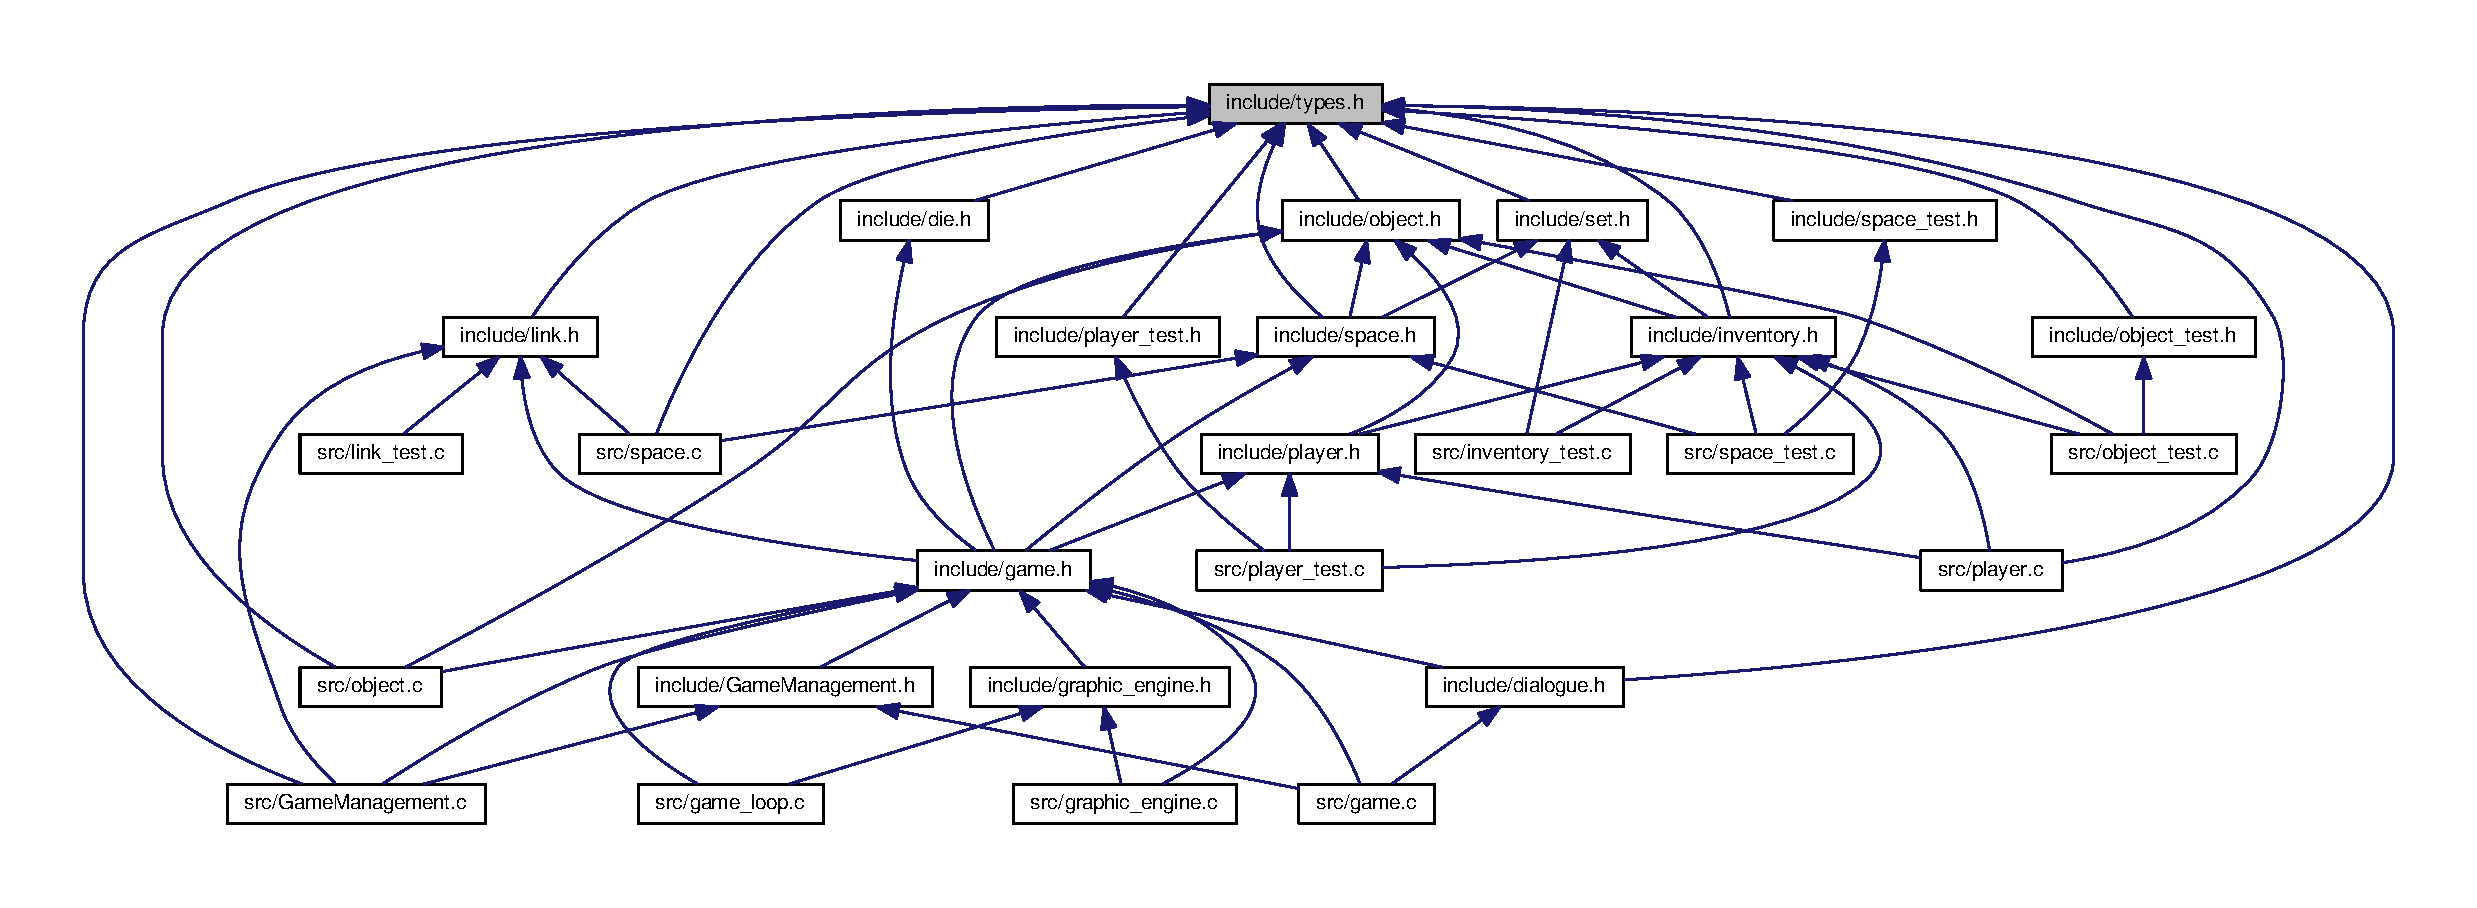
\includegraphics[width=350pt]{types_8h__dep__incl}
\end{center}
\end{figure}
\subsection*{Macros}
\begin{DoxyCompactItemize}
\item 
\#define \hyperlink{types_8h_a92ed8507d1cd2331ad09275c5c4c1c89}{W\+O\+R\+D\+\_\+\+S\+I\+ZE}~1000
\item 
\#define \hyperlink{types_8h_a642e16f35aa1e585c25e405ede76e115}{N\+O\+\_\+\+ID}~-\/1
\item 
\#define \hyperlink{types_8h_a2b9d4cb1200ff8c085b0a4902e0d7229}{M\+A\+X\+\_\+\+D\+E\+S\+C\+R\+I\+P\+T\+I\+ON}~128
\item 
\#define \hyperlink{types_8h_a3a96a0e39038d30582bfa0cf12e87f0c}{M\+A\+X\+\_\+\+L\+O\+N\+G\+\_\+\+D\+E\+S\+C\+R\+I\+P\+T\+I\+ON}~512
\end{DoxyCompactItemize}
\subsection*{Typedefs}
\begin{DoxyCompactItemize}
\item 
typedef long \hyperlink{types_8h_a845e604fb28f7e3d97549da3448149d3}{Id}\hypertarget{types_8h_a845e604fb28f7e3d97549da3448149d3}{}\label{types_8h_a845e604fb28f7e3d97549da3448149d3}

\begin{DoxyCompactList}\small\item\em id\+: long int variable \end{DoxyCompactList}\end{DoxyCompactItemize}
\subsection*{Enumerations}
\begin{DoxyCompactItemize}
\item 
enum \hyperlink{types_8h_a3e5b8192e7d9ffaf3542f1210aec18dd}{B\+O\+OL} \{ \hyperlink{types_8h_a3e5b8192e7d9ffaf3542f1210aec18ddaa1e095cc966dbecf6a0d8aad75348d1a}{F\+A\+L\+SE}, 
\hyperlink{types_8h_a3e5b8192e7d9ffaf3542f1210aec18ddaa82764c3079aea4e60c80e45befbb839}{T\+R\+UE}
 \}\begin{DoxyCompactList}\small\item\em boolean error list \end{DoxyCompactList}
\item 
enum \hyperlink{types_8h_a32c27cc471df37f4fc818d65de0a56c4}{S\+T\+A\+T\+US} \{ \hyperlink{types_8h_a32c27cc471df37f4fc818d65de0a56c4a2fd6f336d08340583bd620a7f5694c90}{E\+R\+R\+OR}, 
\hyperlink{types_8h_a32c27cc471df37f4fc818d65de0a56c4a2bc49ec37d6a5715dd23e85f1ff5bb59}{OK}
 \}\begin{DoxyCompactList}\small\item\em status error list \end{DoxyCompactList}
\item 
enum \hyperlink{types_8h_aa268a41a13430b18e933ed40207178d0}{D\+I\+R\+E\+C\+T\+I\+ON} \{ \hyperlink{types_8h_aa268a41a13430b18e933ed40207178d0a2c63acbe79d9f41ba6bb7766e9c37702}{N}, 
\hyperlink{types_8h_aa268a41a13430b18e933ed40207178d0af1ce01387d2348f8b858721a7db81670}{S}, 
\hyperlink{types_8h_aa268a41a13430b18e933ed40207178d0ab199e021998d49b1f09338d8b9b18ecb}{E}, 
\hyperlink{types_8h_aa268a41a13430b18e933ed40207178d0ab722ceeb601c72cd78fbd35f3581fdf7}{W}
 \}\begin{DoxyCompactList}\small\item\em directons list \end{DoxyCompactList}
\item 
enum \hyperlink{types_8h_a3425906c2a1ce4f324e3b2006ece02cd}{L\+I\+N\+K\+\_\+\+ST} \{ \hyperlink{types_8h_a3425906c2a1ce4f324e3b2006ece02cda0e0143636c29971736eab47415868eae}{O\+P\+EN}, 
\hyperlink{types_8h_a3425906c2a1ce4f324e3b2006ece02cda685f73194ad125cbc784c3210cdb3449}{C\+L\+O\+SE}
 \}\begin{DoxyCompactList}\small\item\em status of link \end{DoxyCompactList}
\end{DoxyCompactItemize}


\subsection{Detailed Description}
Defines some structures and enumerations. 

\begin{DoxyAuthor}{Author}
Juan Moreno 
\end{DoxyAuthor}
\begin{DoxyVersion}{Version}
2.\+0 
\end{DoxyVersion}
\begin{DoxyDate}{Date}
07-\/04-\/2018 
\end{DoxyDate}


\subsection{Macro Definition Documentation}
\index{types.\+h@{types.\+h}!M\+A\+X\+\_\+\+D\+E\+S\+C\+R\+I\+P\+T\+I\+ON@{M\+A\+X\+\_\+\+D\+E\+S\+C\+R\+I\+P\+T\+I\+ON}}
\index{M\+A\+X\+\_\+\+D\+E\+S\+C\+R\+I\+P\+T\+I\+ON@{M\+A\+X\+\_\+\+D\+E\+S\+C\+R\+I\+P\+T\+I\+ON}!types.\+h@{types.\+h}}
\subsubsection[{\texorpdfstring{M\+A\+X\+\_\+\+D\+E\+S\+C\+R\+I\+P\+T\+I\+ON}{MAX_DESCRIPTION}}]{\setlength{\rightskip}{0pt plus 5cm}\#define M\+A\+X\+\_\+\+D\+E\+S\+C\+R\+I\+P\+T\+I\+ON~128}\hypertarget{types_8h_a2b9d4cb1200ff8c085b0a4902e0d7229}{}\label{types_8h_a2b9d4cb1200ff8c085b0a4902e0d7229}
maximum description for an element \index{types.\+h@{types.\+h}!M\+A\+X\+\_\+\+L\+O\+N\+G\+\_\+\+D\+E\+S\+C\+R\+I\+P\+T\+I\+ON@{M\+A\+X\+\_\+\+L\+O\+N\+G\+\_\+\+D\+E\+S\+C\+R\+I\+P\+T\+I\+ON}}
\index{M\+A\+X\+\_\+\+L\+O\+N\+G\+\_\+\+D\+E\+S\+C\+R\+I\+P\+T\+I\+ON@{M\+A\+X\+\_\+\+L\+O\+N\+G\+\_\+\+D\+E\+S\+C\+R\+I\+P\+T\+I\+ON}!types.\+h@{types.\+h}}
\subsubsection[{\texorpdfstring{M\+A\+X\+\_\+\+L\+O\+N\+G\+\_\+\+D\+E\+S\+C\+R\+I\+P\+T\+I\+ON}{MAX_LONG_DESCRIPTION}}]{\setlength{\rightskip}{0pt plus 5cm}\#define M\+A\+X\+\_\+\+L\+O\+N\+G\+\_\+\+D\+E\+S\+C\+R\+I\+P\+T\+I\+ON~512}\hypertarget{types_8h_a3a96a0e39038d30582bfa0cf12e87f0c}{}\label{types_8h_a3a96a0e39038d30582bfa0cf12e87f0c}
maximum description for a long element \index{types.\+h@{types.\+h}!N\+O\+\_\+\+ID@{N\+O\+\_\+\+ID}}
\index{N\+O\+\_\+\+ID@{N\+O\+\_\+\+ID}!types.\+h@{types.\+h}}
\subsubsection[{\texorpdfstring{N\+O\+\_\+\+ID}{NO_ID}}]{\setlength{\rightskip}{0pt plus 5cm}\#define N\+O\+\_\+\+ID~-\/1}\hypertarget{types_8h_a642e16f35aa1e585c25e405ede76e115}{}\label{types_8h_a642e16f35aa1e585c25e405ede76e115}
defines when id is wrong as -\/1 \index{types.\+h@{types.\+h}!W\+O\+R\+D\+\_\+\+S\+I\+ZE@{W\+O\+R\+D\+\_\+\+S\+I\+ZE}}
\index{W\+O\+R\+D\+\_\+\+S\+I\+ZE@{W\+O\+R\+D\+\_\+\+S\+I\+ZE}!types.\+h@{types.\+h}}
\subsubsection[{\texorpdfstring{W\+O\+R\+D\+\_\+\+S\+I\+ZE}{WORD_SIZE}}]{\setlength{\rightskip}{0pt plus 5cm}\#define W\+O\+R\+D\+\_\+\+S\+I\+ZE~1000}\hypertarget{types_8h_a92ed8507d1cd2331ad09275c5c4c1c89}{}\label{types_8h_a92ed8507d1cd2331ad09275c5c4c1c89}
defines a max number for the word 

\subsection{Enumeration Type Documentation}
\index{types.\+h@{types.\+h}!B\+O\+OL@{B\+O\+OL}}
\index{B\+O\+OL@{B\+O\+OL}!types.\+h@{types.\+h}}
\subsubsection[{\texorpdfstring{B\+O\+OL}{BOOL}}]{\setlength{\rightskip}{0pt plus 5cm}enum {\bf B\+O\+OL}}\hypertarget{types_8h_a3e5b8192e7d9ffaf3542f1210aec18dd}{}\label{types_8h_a3e5b8192e7d9ffaf3542f1210aec18dd}


boolean error list 

\begin{Desc}
\item[Enumerator]\par
\begin{description}
\index{F\+A\+L\+SE@{F\+A\+L\+SE}!types.\+h@{types.\+h}}\index{types.\+h@{types.\+h}!F\+A\+L\+SE@{F\+A\+L\+SE}}\item[{\em 
F\+A\+L\+SE\hypertarget{types_8h_a3e5b8192e7d9ffaf3542f1210aec18ddaa1e095cc966dbecf6a0d8aad75348d1a}{}\label{types_8h_a3e5b8192e7d9ffaf3542f1210aec18ddaa1e095cc966dbecf6a0d8aad75348d1a}
}]false condition \index{T\+R\+UE@{T\+R\+UE}!types.\+h@{types.\+h}}\index{types.\+h@{types.\+h}!T\+R\+UE@{T\+R\+UE}}\item[{\em 
T\+R\+UE\hypertarget{types_8h_a3e5b8192e7d9ffaf3542f1210aec18ddaa82764c3079aea4e60c80e45befbb839}{}\label{types_8h_a3e5b8192e7d9ffaf3542f1210aec18ddaa82764c3079aea4e60c80e45befbb839}
}]true condition \end{description}
\end{Desc}
\index{types.\+h@{types.\+h}!D\+I\+R\+E\+C\+T\+I\+ON@{D\+I\+R\+E\+C\+T\+I\+ON}}
\index{D\+I\+R\+E\+C\+T\+I\+ON@{D\+I\+R\+E\+C\+T\+I\+ON}!types.\+h@{types.\+h}}
\subsubsection[{\texorpdfstring{D\+I\+R\+E\+C\+T\+I\+ON}{DIRECTION}}]{\setlength{\rightskip}{0pt plus 5cm}enum {\bf D\+I\+R\+E\+C\+T\+I\+ON}}\hypertarget{types_8h_aa268a41a13430b18e933ed40207178d0}{}\label{types_8h_aa268a41a13430b18e933ed40207178d0}


directons list 

\begin{Desc}
\item[Enumerator]\par
\begin{description}
\index{N@{N}!types.\+h@{types.\+h}}\index{types.\+h@{types.\+h}!N@{N}}\item[{\em 
N\hypertarget{types_8h_aa268a41a13430b18e933ed40207178d0a2c63acbe79d9f41ba6bb7766e9c37702}{}\label{types_8h_aa268a41a13430b18e933ed40207178d0a2c63acbe79d9f41ba6bb7766e9c37702}
}]north direction \index{S@{S}!types.\+h@{types.\+h}}\index{types.\+h@{types.\+h}!S@{S}}\item[{\em 
S\hypertarget{types_8h_aa268a41a13430b18e933ed40207178d0af1ce01387d2348f8b858721a7db81670}{}\label{types_8h_aa268a41a13430b18e933ed40207178d0af1ce01387d2348f8b858721a7db81670}
}]south direction \index{E@{E}!types.\+h@{types.\+h}}\index{types.\+h@{types.\+h}!E@{E}}\item[{\em 
E\hypertarget{types_8h_aa268a41a13430b18e933ed40207178d0ab199e021998d49b1f09338d8b9b18ecb}{}\label{types_8h_aa268a41a13430b18e933ed40207178d0ab199e021998d49b1f09338d8b9b18ecb}
}]east direction \index{W@{W}!types.\+h@{types.\+h}}\index{types.\+h@{types.\+h}!W@{W}}\item[{\em 
W\hypertarget{types_8h_aa268a41a13430b18e933ed40207178d0ab722ceeb601c72cd78fbd35f3581fdf7}{}\label{types_8h_aa268a41a13430b18e933ed40207178d0ab722ceeb601c72cd78fbd35f3581fdf7}
}]west direction \end{description}
\end{Desc}
\index{types.\+h@{types.\+h}!L\+I\+N\+K\+\_\+\+ST@{L\+I\+N\+K\+\_\+\+ST}}
\index{L\+I\+N\+K\+\_\+\+ST@{L\+I\+N\+K\+\_\+\+ST}!types.\+h@{types.\+h}}
\subsubsection[{\texorpdfstring{L\+I\+N\+K\+\_\+\+ST}{LINK_ST}}]{\setlength{\rightskip}{0pt plus 5cm}enum {\bf L\+I\+N\+K\+\_\+\+ST}}\hypertarget{types_8h_a3425906c2a1ce4f324e3b2006ece02cd}{}\label{types_8h_a3425906c2a1ce4f324e3b2006ece02cd}


status of link 

\begin{Desc}
\item[Enumerator]\par
\begin{description}
\index{O\+P\+EN@{O\+P\+EN}!types.\+h@{types.\+h}}\index{types.\+h@{types.\+h}!O\+P\+EN@{O\+P\+EN}}\item[{\em 
O\+P\+EN\hypertarget{types_8h_a3425906c2a1ce4f324e3b2006ece02cda0e0143636c29971736eab47415868eae}{}\label{types_8h_a3425906c2a1ce4f324e3b2006ece02cda0e0143636c29971736eab47415868eae}
}]opened link \index{C\+L\+O\+SE@{C\+L\+O\+SE}!types.\+h@{types.\+h}}\index{types.\+h@{types.\+h}!C\+L\+O\+SE@{C\+L\+O\+SE}}\item[{\em 
C\+L\+O\+SE\hypertarget{types_8h_a3425906c2a1ce4f324e3b2006ece02cda685f73194ad125cbc784c3210cdb3449}{}\label{types_8h_a3425906c2a1ce4f324e3b2006ece02cda685f73194ad125cbc784c3210cdb3449}
}]closed link \end{description}
\end{Desc}
\index{types.\+h@{types.\+h}!S\+T\+A\+T\+US@{S\+T\+A\+T\+US}}
\index{S\+T\+A\+T\+US@{S\+T\+A\+T\+US}!types.\+h@{types.\+h}}
\subsubsection[{\texorpdfstring{S\+T\+A\+T\+US}{STATUS}}]{\setlength{\rightskip}{0pt plus 5cm}enum {\bf S\+T\+A\+T\+US}}\hypertarget{types_8h_a32c27cc471df37f4fc818d65de0a56c4}{}\label{types_8h_a32c27cc471df37f4fc818d65de0a56c4}


status error list 

\begin{Desc}
\item[Enumerator]\par
\begin{description}
\index{E\+R\+R\+OR@{E\+R\+R\+OR}!types.\+h@{types.\+h}}\index{types.\+h@{types.\+h}!E\+R\+R\+OR@{E\+R\+R\+OR}}\item[{\em 
E\+R\+R\+OR\hypertarget{types_8h_a32c27cc471df37f4fc818d65de0a56c4a2fd6f336d08340583bd620a7f5694c90}{}\label{types_8h_a32c27cc471df37f4fc818d65de0a56c4a2fd6f336d08340583bd620a7f5694c90}
}]error \index{OK@{OK}!types.\+h@{types.\+h}}\index{types.\+h@{types.\+h}!OK@{OK}}\item[{\em 
OK\hypertarget{types_8h_a32c27cc471df37f4fc818d65de0a56c4a2bc49ec37d6a5715dd23e85f1ff5bb59}{}\label{types_8h_a32c27cc471df37f4fc818d65de0a56c4a2bc49ec37d6a5715dd23e85f1ff5bb59}
}]No error \end{description}
\end{Desc}

\hypertarget{game_8c}{}\section{src/game.c File Reference}
\label{game_8c}\index{src/game.\+c@{src/game.\+c}}


Defines the game module.  


{\ttfamily \#include $<$stdio.\+h$>$}\\*
{\ttfamily \#include $<$stdlib.\+h$>$}\\*
{\ttfamily \#include $<$string.\+h$>$}\\*
{\ttfamily \#include $<$strings.\+h$>$}\\*
{\ttfamily \#include $<$time.\+h$>$}\\*
{\ttfamily \#include \char`\"{}game.\+h\char`\"{}}\\*
{\ttfamily \#include \char`\"{}Game\+Management.\+h\char`\"{}}\\*
{\ttfamily \#include \char`\"{}dialogue.\+h\char`\"{}}\\*
Include dependency graph for game.\+c\+:
\nopagebreak
\begin{figure}[H]
\begin{center}
\leavevmode
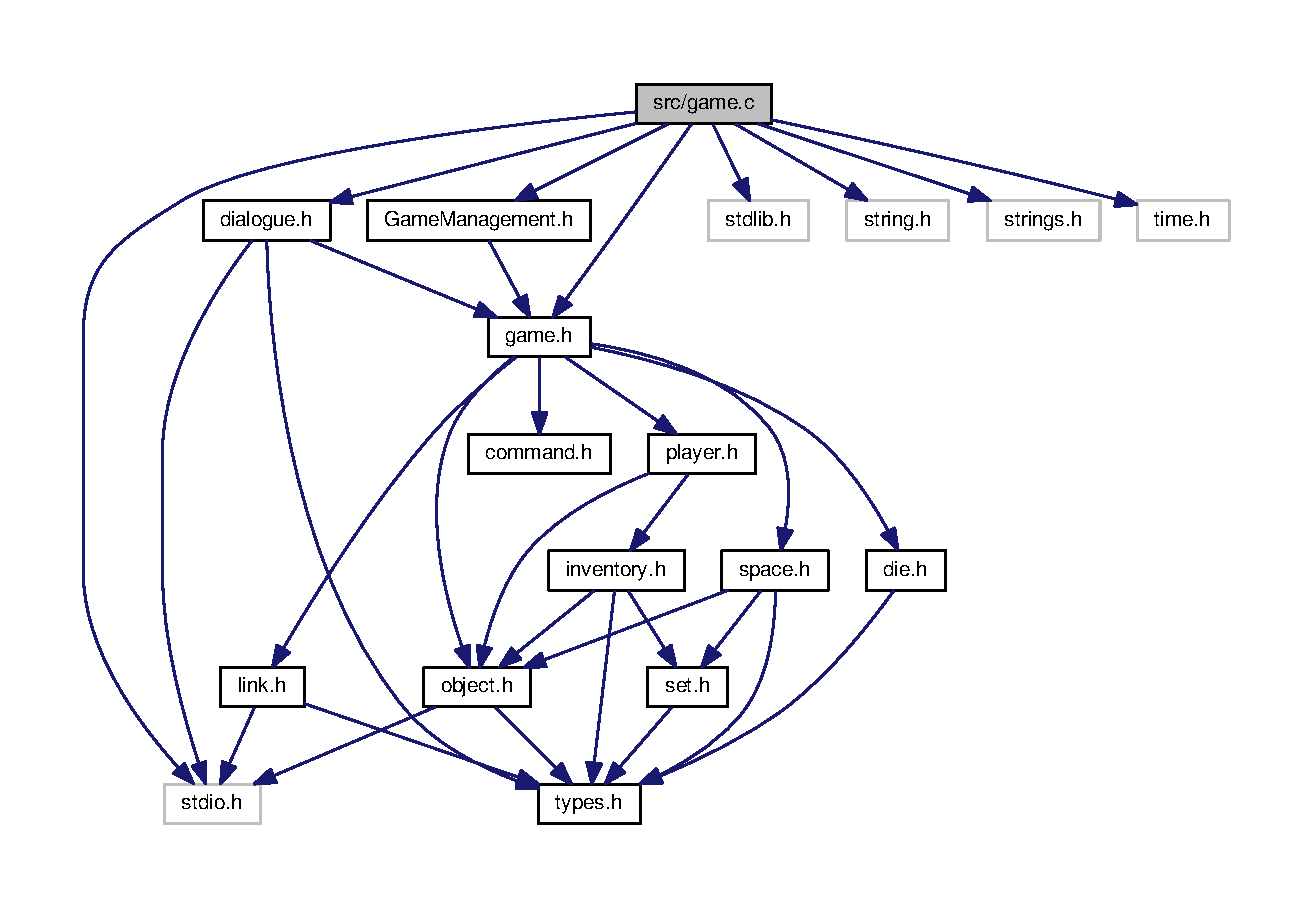
\includegraphics[width=350pt]{game_8c__incl}
\end{center}
\end{figure}
\subsection*{Data Structures}
\begin{DoxyCompactItemize}
\item 
struct \hyperlink{struct__Game}{\+\_\+\+Game}
\begin{DoxyCompactList}\small\item\em game definition \end{DoxyCompactList}\end{DoxyCompactItemize}
\subsection*{Macros}
\begin{DoxyCompactItemize}
\item 
\#define \hyperlink{game_8c_a8366e5ad74afbbea0cd0a414770c304a}{N\+\_\+\+C\+A\+L\+L\+B\+A\+CK}~12
\end{DoxyCompactItemize}
\subsection*{Typedefs}
\begin{DoxyCompactItemize}
\item 
typedef void($\ast$ \hyperlink{game_8c_ac54a175bdefaeb274c3515fc6f43dbe5}{callback\+\_\+fn}) (\hyperlink{game_8h_a57156d39c530aec3fba3a9dad8c2dc6a}{Game} $\ast$game)
\end{DoxyCompactItemize}
\subsection*{Functions}
\begin{DoxyCompactItemize}
\item 
void \hyperlink{game_8c_ac8ed327ed13f97dcb778d0293f14d8bb}{game\+\_\+callback\+\_\+unknown} (\hyperlink{game_8h_a57156d39c530aec3fba3a9dad8c2dc6a}{Game} $\ast$game)
\begin{DoxyCompactList}\small\item\em creates the \char`\"{}unknown\char`\"{} command \end{DoxyCompactList}\item 
void \hyperlink{game_8c_acc98d79a418d2093fc3224b5c02e5418}{game\+\_\+callback\+\_\+exit} (\hyperlink{game_8h_a57156d39c530aec3fba3a9dad8c2dc6a}{Game} $\ast$game)
\begin{DoxyCompactList}\small\item\em creates the \char`\"{}exit\char`\"{} command \end{DoxyCompactList}\item 
void \hyperlink{game_8c_a3553183763f9ee16ae77052056a284b1}{game\+\_\+callback\+\_\+grasp} (\hyperlink{game_8h_a57156d39c530aec3fba3a9dad8c2dc6a}{Game} $\ast$game)
\begin{DoxyCompactList}\small\item\em creates the \char`\"{}grasp\char`\"{} command \end{DoxyCompactList}\item 
void \hyperlink{game_8c_a424d0c659a926b0588a4287ea82552b6}{game\+\_\+callback\+\_\+drop} (\hyperlink{game_8h_a57156d39c530aec3fba3a9dad8c2dc6a}{Game} $\ast$game)
\begin{DoxyCompactList}\small\item\em creates the \char`\"{}drop\char`\"{} command \end{DoxyCompactList}\item 
void \hyperlink{game_8c_a58b275b26a64926b39f498a163d9f22a}{game\+\_\+callback\+\_\+throw} (\hyperlink{game_8h_a57156d39c530aec3fba3a9dad8c2dc6a}{Game} $\ast$game)
\begin{DoxyCompactList}\small\item\em creates the \char`\"{}throw\char`\"{} command \end{DoxyCompactList}\item 
void \hyperlink{game_8c_a83bb67a81f8905d8aebdc441fd23325b}{game\+\_\+callback\+\_\+check} (\hyperlink{game_8h_a57156d39c530aec3fba3a9dad8c2dc6a}{Game} $\ast$game)
\begin{DoxyCompactList}\small\item\em description of elements. \end{DoxyCompactList}\item 
void \hyperlink{game_8c_a7525cbe807f8d1c3b698afcb75903903}{game\+\_\+callback\+\_\+move} (\hyperlink{game_8h_a57156d39c530aec3fba3a9dad8c2dc6a}{Game} $\ast$game)
\begin{DoxyCompactList}\small\item\em command that moves an object \end{DoxyCompactList}\item 
void \hyperlink{game_8c_a0d129f4633cdfeae4332360ba00c0c6d}{game\+\_\+callback\+\_\+turnon} (\hyperlink{game_8h_a57156d39c530aec3fba3a9dad8c2dc6a}{Game} $\ast$game)
\begin{DoxyCompactList}\small\item\em creates de \char`\"{}turn on command\char`\"{}. \end{DoxyCompactList}\item 
void \hyperlink{game_8c_a3f840da3cd6ce1b3273dd5b83719503d}{game\+\_\+callback\+\_\+turnoff} (\hyperlink{game_8h_a57156d39c530aec3fba3a9dad8c2dc6a}{Game} $\ast$game)
\begin{DoxyCompactList}\small\item\em creates de \char`\"{}turn off command\char`\"{}. \end{DoxyCompactList}\item 
void \hyperlink{game_8c_affcf55da4331b7a9e41ca8b791db317c}{game\+\_\+callback\+\_\+unlock} (\hyperlink{game_8h_a57156d39c530aec3fba3a9dad8c2dc6a}{Game} $\ast$game)
\begin{DoxyCompactList}\small\item\em creates de \char`\"{}unlock\char`\"{} command. \end{DoxyCompactList}\item 
void \hyperlink{game_8c_a92370dabeae0c2075c3f0677d3afe3df}{game\+\_\+callback\+\_\+save} (\hyperlink{game_8h_a57156d39c530aec3fba3a9dad8c2dc6a}{Game} $\ast$game)
\begin{DoxyCompactList}\small\item\em creates de \char`\"{}save\char`\"{} command. \end{DoxyCompactList}\item 
void \hyperlink{game_8c_ad933ddba178af5ab5f5c79abc108996f}{game\+\_\+callback\+\_\+load} (\hyperlink{game_8h_a57156d39c530aec3fba3a9dad8c2dc6a}{Game} $\ast$game)
\begin{DoxyCompactList}\small\item\em creates de \char`\"{}load\char`\"{} command. \end{DoxyCompactList}\item 
\hyperlink{types_8h_a32c27cc471df37f4fc818d65de0a56c4}{S\+T\+A\+T\+US} \hyperlink{game_8c_ae5ad86de0a92d9eccb234948458da7f1}{game\+\_\+add\+\_\+space} (\hyperlink{game_8h_a57156d39c530aec3fba3a9dad8c2dc6a}{Game} $\ast$game, \hyperlink{space_8h_a67533ffc2b70463baecc38fb0629bbfc}{Space} $\ast$space)
\begin{DoxyCompactList}\small\item\em adds a space \end{DoxyCompactList}\item 
\hyperlink{types_8h_a845e604fb28f7e3d97549da3448149d3}{Id} \hyperlink{game_8c_ad2dfd865e2bd2c545a15d33f4d1cf3ae}{game\+\_\+get\+\_\+space\+\_\+id\+\_\+at} (\hyperlink{game_8h_a57156d39c530aec3fba3a9dad8c2dc6a}{Game} $\ast$game, int position)
\begin{DoxyCompactList}\small\item\em gets and id \end{DoxyCompactList}\item 
\hyperlink{types_8h_a32c27cc471df37f4fc818d65de0a56c4}{S\+T\+A\+T\+US} \hyperlink{game_8c_a492ca9fb594442dc43fc7d18a3820426}{game\+\_\+set\+\_\+player\+\_\+location} (\hyperlink{game_8h_a57156d39c530aec3fba3a9dad8c2dc6a}{Game} $\ast$game, \hyperlink{types_8h_a845e604fb28f7e3d97549da3448149d3}{Id} id)
\begin{DoxyCompactList}\small\item\em sets location \end{DoxyCompactList}\item 
\hyperlink{game_8h_a57156d39c530aec3fba3a9dad8c2dc6a}{Game} $\ast$ \hyperlink{game_8c_a1cdbe3f06b9bf49eb5e334a22ad3b2b9}{game\+\_\+create} ()
\begin{DoxyCompactList}\small\item\em creates a game \end{DoxyCompactList}\item 
\hyperlink{types_8h_a32c27cc471df37f4fc818d65de0a56c4}{S\+T\+A\+T\+US} \hyperlink{game_8c_afc77f90739be0fd45b7f5616e543bfae}{game\+\_\+create\+\_\+from\+\_\+file} (\hyperlink{game_8h_a57156d39c530aec3fba3a9dad8c2dc6a}{Game} $\ast$game, char $\ast$filename)
\begin{DoxyCompactList}\small\item\em calls the game\+\_\+reader functions \end{DoxyCompactList}\item 
\hyperlink{types_8h_a32c27cc471df37f4fc818d65de0a56c4}{S\+T\+A\+T\+US} \hyperlink{game_8c_a0736924a1235c0e6fe9b6d91c2a12af8}{game\+\_\+destroy} (\hyperlink{game_8h_a57156d39c530aec3fba3a9dad8c2dc6a}{Game} $\ast$game)
\begin{DoxyCompactList}\small\item\em Frees the memory of all the elements in a game. \end{DoxyCompactList}\item 
\hyperlink{types_8h_a32c27cc471df37f4fc818d65de0a56c4}{S\+T\+A\+T\+US} \hyperlink{game_8c_a9597a8e456aa74db536e87d56f56c3b4}{game\+\_\+add\+\_\+object} (\hyperlink{game_8h_a57156d39c530aec3fba3a9dad8c2dc6a}{Game} $\ast$game, \hyperlink{object_8h_a7f8bbcda919b65ce67f92fba08e0212f}{Object} $\ast$object)
\begin{DoxyCompactList}\small\item\em adds an object to the game \end{DoxyCompactList}\item 
\hyperlink{space_8h_a67533ffc2b70463baecc38fb0629bbfc}{Space} $\ast$ \hyperlink{game_8c_a69d94da9d27b542d3ebdeb8b60f1f2dc}{game\+\_\+get\+\_\+space} (\hyperlink{game_8h_a57156d39c530aec3fba3a9dad8c2dc6a}{Game} $\ast$game, \hyperlink{types_8h_a845e604fb28f7e3d97549da3448149d3}{Id} id)
\begin{DoxyCompactList}\small\item\em gets the spaces of the game \end{DoxyCompactList}\item 
\hyperlink{types_8h_a32c27cc471df37f4fc818d65de0a56c4}{S\+T\+A\+T\+US} \hyperlink{game_8c_a7376b540583e0df561780afe83a82370}{game\+\_\+set\+\_\+object\+\_\+location} (\hyperlink{object_8h_a7f8bbcda919b65ce67f92fba08e0212f}{Object} $\ast$object, \hyperlink{types_8h_a845e604fb28f7e3d97549da3448149d3}{Id} id)
\begin{DoxyCompactList}\small\item\em sets a location for an object \end{DoxyCompactList}\item 
\hyperlink{types_8h_a845e604fb28f7e3d97549da3448149d3}{Id} \hyperlink{game_8c_ac6a628f2106f81c37d0e83c67920615f}{game\+\_\+get\+\_\+player\+\_\+location} (\hyperlink{game_8h_a57156d39c530aec3fba3a9dad8c2dc6a}{Game} $\ast$game)
\begin{DoxyCompactList}\small\item\em gets the location of the player \end{DoxyCompactList}\item 
\hyperlink{types_8h_a845e604fb28f7e3d97549da3448149d3}{Id} \hyperlink{game_8c_a7825a43a120a5240133cd4c09f5364e1}{game\+\_\+get\+\_\+object\+\_\+location} (\hyperlink{object_8h_a7f8bbcda919b65ce67f92fba08e0212f}{Object} $\ast$object)
\begin{DoxyCompactList}\small\item\em gets the location of an object \end{DoxyCompactList}\item 
int \hyperlink{game_8c_a8726102792afb740eb8e654d933b1cc1}{game\+\_\+get\+\_\+die\+\_\+lastroll} (\hyperlink{game_8h_a57156d39c530aec3fba3a9dad8c2dc6a}{Game} $\ast$game)
\begin{DoxyCompactList}\small\item\em gets the last value of the die \end{DoxyCompactList}\item 
\hyperlink{types_8h_a32c27cc471df37f4fc818d65de0a56c4}{S\+T\+A\+T\+US} \hyperlink{game_8c_a005b4f436300333e7fff8fba2027337e}{game\+\_\+update} (\hyperlink{game_8h_a57156d39c530aec3fba3a9dad8c2dc6a}{Game} $\ast$game, \hyperlink{command_8h_a0473597db8c45c0289b6b8e2f8abbe32}{T\+\_\+\+Command} cmd)
\begin{DoxyCompactList}\small\item\em executes commands \end{DoxyCompactList}\item 
\hyperlink{command_8h_a0473597db8c45c0289b6b8e2f8abbe32}{T\+\_\+\+Command} \hyperlink{game_8c_ac35df1afdade2b7659ebbcfeca1f0c35}{game\+\_\+get\+\_\+last\+\_\+command} (\hyperlink{game_8h_a57156d39c530aec3fba3a9dad8c2dc6a}{Game} $\ast$game)
\begin{DoxyCompactList}\small\item\em gets the last command selected \end{DoxyCompactList}\item 
\hyperlink{types_8h_a32c27cc471df37f4fc818d65de0a56c4}{S\+T\+A\+T\+US} \hyperlink{game_8c_abb8b884baa9dc2d492f60210e827f5dd}{game\+\_\+get\+\_\+last\+\_\+command\+\_\+status} (\hyperlink{game_8h_a57156d39c530aec3fba3a9dad8c2dc6a}{Game} $\ast$game)
\begin{DoxyCompactList}\small\item\em gets the last command \end{DoxyCompactList}\item 
void \hyperlink{game_8c_a33a5ed8937423f8c012df3cedad4fa4c}{game\+\_\+print\+\_\+data} (\hyperlink{game_8h_a57156d39c530aec3fba3a9dad8c2dc6a}{Game} $\ast$game)
\begin{DoxyCompactList}\small\item\em prints the data of the game \end{DoxyCompactList}\item 
\hyperlink{types_8h_a3e5b8192e7d9ffaf3542f1210aec18dd}{B\+O\+OL} \hyperlink{game_8c_aa6efe0650af110bbd84e742cc8046d93}{game\+\_\+is\+\_\+over} (\hyperlink{game_8h_a57156d39c530aec3fba3a9dad8c2dc6a}{Game} $\ast$game)
\begin{DoxyCompactList}\small\item\em Checks if the game has ended. \end{DoxyCompactList}\item 
\hyperlink{object_8h_a7f8bbcda919b65ce67f92fba08e0212f}{Object} $\ast$ \hyperlink{game_8c_a286c704414005130dab85638f34ca48d}{get\+\_\+object\+\_\+from\+\_\+game} (\hyperlink{game_8h_a57156d39c530aec3fba3a9dad8c2dc6a}{Game} $\ast$game, int i)
\begin{DoxyCompactList}\small\item\em gets and object from the game \end{DoxyCompactList}\item 
\hyperlink{player_8h_af30e2030635a69690f85e48bc6ef202f}{Player} $\ast$ \hyperlink{game_8c_a7ea36d7b226f6ff5196214524b296557}{get\+\_\+player\+\_\+from\+\_\+game} (\hyperlink{game_8h_a57156d39c530aec3fba3a9dad8c2dc6a}{Game} $\ast$game)
\begin{DoxyCompactList}\small\item\em gets the player \end{DoxyCompactList}\item 
char $\ast$ \hyperlink{game_8c_a0c9027fd711bd96429bee8fdfc964493}{game\+\_\+get\+\_\+aux} (\hyperlink{game_8h_a57156d39c530aec3fba3a9dad8c2dc6a}{Game} $\ast$game)
\begin{DoxyCompactList}\small\item\em gets an auxiliary string \end{DoxyCompactList}\item 
\hyperlink{types_8h_a32c27cc471df37f4fc818d65de0a56c4}{S\+T\+A\+T\+US} \hyperlink{game_8c_a4691bee17d5784ad6eb257dfbb252c27}{game\+\_\+add\+\_\+link} (\hyperlink{game_8h_a57156d39c530aec3fba3a9dad8c2dc6a}{Game} $\ast$game, \hyperlink{link_8h_ae3b299941e67be6971bfd64a25505eff}{Link} $\ast$link)
\begin{DoxyCompactList}\small\item\em adds a link to the game \end{DoxyCompactList}\item 
\hyperlink{link_8h_ae3b299941e67be6971bfd64a25505eff}{Link} $\ast$ \hyperlink{game_8c_a1064ec927b8c33cf55982b73845db7d3}{game\+\_\+get\+\_\+link} (\hyperlink{game_8h_a57156d39c530aec3fba3a9dad8c2dc6a}{Game} $\ast$game, \hyperlink{types_8h_a845e604fb28f7e3d97549da3448149d3}{Id} id)
\begin{DoxyCompactList}\small\item\em gets link of the game \end{DoxyCompactList}\item 
\hyperlink{die_8h_a892f0b0bf81d69a1f7a14ea238e36dd3}{Die} $\ast$ \hyperlink{game_8c_acfa528e54998d1b0e522d20b59c548e5}{get\+\_\+die\+\_\+from\+\_\+game} (\hyperlink{game_8h_a57156d39c530aec3fba3a9dad8c2dc6a}{Game} $\ast$game)
\begin{DoxyCompactList}\small\item\em gets die of the game \end{DoxyCompactList}\end{DoxyCompactItemize}


\subsection{Detailed Description}
Defines the game module. 

It implements the game interface and all the associated callbacks for each command.

\begin{DoxyAuthor}{Author}
Juan Moreno 
\end{DoxyAuthor}
\begin{DoxyVersion}{Version}
2.\+4 
\end{DoxyVersion}
\begin{DoxyDate}{Date}
07-\/04-\/2018 
\end{DoxyDate}


\subsection{Macro Definition Documentation}
\index{game.\+c@{game.\+c}!N\+\_\+\+C\+A\+L\+L\+B\+A\+CK@{N\+\_\+\+C\+A\+L\+L\+B\+A\+CK}}
\index{N\+\_\+\+C\+A\+L\+L\+B\+A\+CK@{N\+\_\+\+C\+A\+L\+L\+B\+A\+CK}!game.\+c@{game.\+c}}
\subsubsection[{\texorpdfstring{N\+\_\+\+C\+A\+L\+L\+B\+A\+CK}{N_CALLBACK}}]{\setlength{\rightskip}{0pt plus 5cm}\#define N\+\_\+\+C\+A\+L\+L\+B\+A\+CK~12}\hypertarget{game_8c_a8366e5ad74afbbea0cd0a414770c304a}{}\label{game_8c_a8366e5ad74afbbea0cd0a414770c304a}
Number of callback functions 

\subsection{Typedef Documentation}
\index{game.\+c@{game.\+c}!callback\+\_\+fn@{callback\+\_\+fn}}
\index{callback\+\_\+fn@{callback\+\_\+fn}!game.\+c@{game.\+c}}
\subsubsection[{\texorpdfstring{callback\+\_\+fn}{callback_fn}}]{\setlength{\rightskip}{0pt plus 5cm}typedef void($\ast$ callback\+\_\+fn) ({\bf Game} $\ast$game)}\hypertarget{game_8c_ac54a175bdefaeb274c3515fc6f43dbe5}{}\label{game_8c_ac54a175bdefaeb274c3515fc6f43dbe5}
Define the function type for the callbacks 

\subsection{Function Documentation}
\index{game.\+c@{game.\+c}!game\+\_\+add\+\_\+link@{game\+\_\+add\+\_\+link}}
\index{game\+\_\+add\+\_\+link@{game\+\_\+add\+\_\+link}!game.\+c@{game.\+c}}
\subsubsection[{\texorpdfstring{game\+\_\+add\+\_\+link(\+Game $\ast$game, Link $\ast$link)}{game_add_link(Game *game, Link *link)}}]{\setlength{\rightskip}{0pt plus 5cm}{\bf S\+T\+A\+T\+US} game\+\_\+add\+\_\+link (
\begin{DoxyParamCaption}
\item[{{\bf Game} $\ast$}]{game, }
\item[{{\bf Link} $\ast$}]{link}
\end{DoxyParamCaption}
)}\hypertarget{game_8c_a4691bee17d5784ad6eb257dfbb252c27}{}\label{game_8c_a4691bee17d5784ad6eb257dfbb252c27}


adds a link to the game 

It is the function in charge of adding links to the game when considering it appropriate.

\begin{DoxyAuthor}{Author}
Juan Moreno 
\end{DoxyAuthor}

\begin{DoxyParams}{Parameters}
{\em game} & pointer to game. \\
\hline
{\em link} & pointer to link \\
\hline
\end{DoxyParams}
\begin{DoxyReturn}{Returns}
S\+T\+A\+T\+US, E\+R\+R\+OR if argument received is N\+U\+LL, if not, OK. 
\end{DoxyReturn}
\index{game.\+c@{game.\+c}!game\+\_\+add\+\_\+object@{game\+\_\+add\+\_\+object}}
\index{game\+\_\+add\+\_\+object@{game\+\_\+add\+\_\+object}!game.\+c@{game.\+c}}
\subsubsection[{\texorpdfstring{game\+\_\+add\+\_\+object(\+Game $\ast$game, Object $\ast$object)}{game_add_object(Game *game, Object *object)}}]{\setlength{\rightskip}{0pt plus 5cm}{\bf S\+T\+A\+T\+US} game\+\_\+add\+\_\+object (
\begin{DoxyParamCaption}
\item[{{\bf Game} $\ast$}]{game, }
\item[{{\bf Object} $\ast$}]{object}
\end{DoxyParamCaption}
)}\hypertarget{game_8c_a9597a8e456aa74db536e87d56f56c3b4}{}\label{game_8c_a9597a8e456aa74db536e87d56f56c3b4}


adds an object to the game 

\begin{DoxyAuthor}{Author}
Juan Moreno 
\end{DoxyAuthor}

\begin{DoxyParams}{Parameters}
{\em game} & pointer to game. \\
\hline
{\em object} & pointer to object. \\
\hline
\end{DoxyParams}
\begin{DoxyReturn}{Returns}
S\+T\+A\+T\+US, E\+R\+R\+OR if argument received is N\+U\+LL, if not, OK. 
\end{DoxyReturn}
\index{game.\+c@{game.\+c}!game\+\_\+add\+\_\+space@{game\+\_\+add\+\_\+space}}
\index{game\+\_\+add\+\_\+space@{game\+\_\+add\+\_\+space}!game.\+c@{game.\+c}}
\subsubsection[{\texorpdfstring{game\+\_\+add\+\_\+space(\+Game $\ast$game, Space $\ast$space)}{game_add_space(Game *game, Space *space)}}]{\setlength{\rightskip}{0pt plus 5cm}{\bf S\+T\+A\+T\+US} game\+\_\+add\+\_\+space (
\begin{DoxyParamCaption}
\item[{{\bf Game} $\ast$}]{game, }
\item[{{\bf Space} $\ast$}]{space}
\end{DoxyParamCaption}
)}\hypertarget{game_8c_ae5ad86de0a92d9eccb234948458da7f1}{}\label{game_8c_ae5ad86de0a92d9eccb234948458da7f1}


adds a space 

adds a space to the game

Private functions Function that implements spaces by using the set module to add values.

\begin{DoxyAuthor}{Author}
Juan Moreno 
\end{DoxyAuthor}

\begin{DoxyParams}{Parameters}
{\em game} & pointer to game. \\
\hline
{\em space} & pointer to space. \\
\hline
\end{DoxyParams}
\begin{DoxyReturn}{Returns}
S\+T\+A\+T\+US, E\+R\+R\+OR if argument received is N\+U\+LL, if not, OK. 
\end{DoxyReturn}
\index{game.\+c@{game.\+c}!game\+\_\+callback\+\_\+check@{game\+\_\+callback\+\_\+check}}
\index{game\+\_\+callback\+\_\+check@{game\+\_\+callback\+\_\+check}!game.\+c@{game.\+c}}
\subsubsection[{\texorpdfstring{game\+\_\+callback\+\_\+check(\+Game $\ast$game)}{game_callback_check(Game *game)}}]{\setlength{\rightskip}{0pt plus 5cm}void game\+\_\+callback\+\_\+check (
\begin{DoxyParamCaption}
\item[{{\bf Game} $\ast$}]{game}
\end{DoxyParamCaption}
)}\hypertarget{game_8c_a83bb67a81f8905d8aebdc441fd23325b}{}\label{game_8c_a83bb67a81f8905d8aebdc441fd23325b}


description of elements. 

When checking a principal element of the game, it shows a description of the element you choose.

\begin{DoxyAuthor}{Author}
Juan Moreno 
\end{DoxyAuthor}

\begin{DoxyParams}{Parameters}
{\em game} & pointer to game. \\
\hline
\end{DoxyParams}
\begin{DoxyReturn}{Returns}
void function. 
\end{DoxyReturn}
\index{game.\+c@{game.\+c}!game\+\_\+callback\+\_\+drop@{game\+\_\+callback\+\_\+drop}}
\index{game\+\_\+callback\+\_\+drop@{game\+\_\+callback\+\_\+drop}!game.\+c@{game.\+c}}
\subsubsection[{\texorpdfstring{game\+\_\+callback\+\_\+drop(\+Game $\ast$game)}{game_callback_drop(Game *game)}}]{\setlength{\rightskip}{0pt plus 5cm}void game\+\_\+callback\+\_\+drop (
\begin{DoxyParamCaption}
\item[{{\bf Game} $\ast$}]{game}
\end{DoxyParamCaption}
)}\hypertarget{game_8c_a424d0c659a926b0588a4287ea82552b6}{}\label{game_8c_a424d0c659a926b0588a4287ea82552b6}


creates the \char`\"{}drop\char`\"{} command 

If the player is not holding any objects, or the space hasnt loaded correctly ends the execution, if not reactivates the object in game adds the object to the space set and deletes the player\textquotesingle{}s object

\begin{DoxyAuthor}{Author}
Juan Moreno 
\end{DoxyAuthor}

\begin{DoxyParams}{Parameters}
{\em game} & pointer to game. \\
\hline
\end{DoxyParams}
\begin{DoxyReturn}{Returns}
void function. 
\end{DoxyReturn}
\index{game.\+c@{game.\+c}!game\+\_\+callback\+\_\+exit@{game\+\_\+callback\+\_\+exit}}
\index{game\+\_\+callback\+\_\+exit@{game\+\_\+callback\+\_\+exit}!game.\+c@{game.\+c}}
\subsubsection[{\texorpdfstring{game\+\_\+callback\+\_\+exit(\+Game $\ast$game)}{game_callback_exit(Game *game)}}]{\setlength{\rightskip}{0pt plus 5cm}void game\+\_\+callback\+\_\+exit (
\begin{DoxyParamCaption}
\item[{{\bf Game} $\ast$}]{game}
\end{DoxyParamCaption}
)}\hypertarget{game_8c_acc98d79a418d2093fc3224b5c02e5418}{}\label{game_8c_acc98d79a418d2093fc3224b5c02e5418}


creates the \char`\"{}exit\char`\"{} command 

Exits the game when command is selected.

\begin{DoxyAuthor}{Author}
Juan Moreno 
\end{DoxyAuthor}
\begin{DoxyReturn}{Returns}
void function. 
\end{DoxyReturn}
\index{game.\+c@{game.\+c}!game\+\_\+callback\+\_\+grasp@{game\+\_\+callback\+\_\+grasp}}
\index{game\+\_\+callback\+\_\+grasp@{game\+\_\+callback\+\_\+grasp}!game.\+c@{game.\+c}}
\subsubsection[{\texorpdfstring{game\+\_\+callback\+\_\+grasp(\+Game $\ast$game)}{game_callback_grasp(Game *game)}}]{\setlength{\rightskip}{0pt plus 5cm}void game\+\_\+callback\+\_\+grasp (
\begin{DoxyParamCaption}
\item[{{\bf Game} $\ast$}]{game}
\end{DoxyParamCaption}
)}\hypertarget{game_8c_a3553183763f9ee16ae77052056a284b1}{}\label{game_8c_a3553183763f9ee16ae77052056a284b1}


creates the \char`\"{}grasp\char`\"{} command 

First asks for an object name in the graphic engine\textquotesingle{}s command terminal, then if the player is already holding an object, the object requested doesnt exist in that space or the space hasnt loaded correctly ends. If not, moves the object to a special space recorded as player inventory (-\/7), copies the object in the player object and deletes the object from the set in the space.

\begin{DoxyAuthor}{Author}
Juan Moreno 
\end{DoxyAuthor}

\begin{DoxyParams}{Parameters}
{\em game} & pointer to game. \\
\hline
\end{DoxyParams}
\begin{DoxyReturn}{Returns}
void function. 
\end{DoxyReturn}
\index{game.\+c@{game.\+c}!game\+\_\+callback\+\_\+load@{game\+\_\+callback\+\_\+load}}
\index{game\+\_\+callback\+\_\+load@{game\+\_\+callback\+\_\+load}!game.\+c@{game.\+c}}
\subsubsection[{\texorpdfstring{game\+\_\+callback\+\_\+load(\+Game $\ast$game)}{game_callback_load(Game *game)}}]{\setlength{\rightskip}{0pt plus 5cm}void game\+\_\+callback\+\_\+load (
\begin{DoxyParamCaption}
\item[{{\bf Game} $\ast$}]{game}
\end{DoxyParamCaption}
)}\hypertarget{game_8c_ad933ddba178af5ab5f5c79abc108996f}{}\label{game_8c_ad933ddba178af5ab5f5c79abc108996f}


creates de \char`\"{}load\char`\"{} command. 

It creates the command that enables us to load games that have already been saved.

\begin{DoxyAuthor}{Author}
Juan Moreno 
\end{DoxyAuthor}

\begin{DoxyParams}{Parameters}
{\em game} & pointer to game. \\
\hline
\end{DoxyParams}
\begin{DoxyReturn}{Returns}
void function. 
\end{DoxyReturn}
\index{game.\+c@{game.\+c}!game\+\_\+callback\+\_\+move@{game\+\_\+callback\+\_\+move}}
\index{game\+\_\+callback\+\_\+move@{game\+\_\+callback\+\_\+move}!game.\+c@{game.\+c}}
\subsubsection[{\texorpdfstring{game\+\_\+callback\+\_\+move(\+Game $\ast$game)}{game_callback_move(Game *game)}}]{\setlength{\rightskip}{0pt plus 5cm}void game\+\_\+callback\+\_\+move (
\begin{DoxyParamCaption}
\item[{{\bf Game} $\ast$}]{game}
\end{DoxyParamCaption}
)}\hypertarget{game_8c_a7525cbe807f8d1c3b698afcb75903903}{}\label{game_8c_a7525cbe807f8d1c3b698afcb75903903}


command that moves an object 

It is the function in charge of linking the commands \char`\"{}following\char`\"{} and \char`\"{}previous\char`\"{}.

\begin{DoxyAuthor}{Author}
Juan Moreno 
\end{DoxyAuthor}

\begin{DoxyParams}{Parameters}
{\em game} & pointer to game. \\
\hline
\end{DoxyParams}
\begin{DoxyReturn}{Returns}
void function. 
\end{DoxyReturn}
\index{game.\+c@{game.\+c}!game\+\_\+callback\+\_\+save@{game\+\_\+callback\+\_\+save}}
\index{game\+\_\+callback\+\_\+save@{game\+\_\+callback\+\_\+save}!game.\+c@{game.\+c}}
\subsubsection[{\texorpdfstring{game\+\_\+callback\+\_\+save(\+Game $\ast$game)}{game_callback_save(Game *game)}}]{\setlength{\rightskip}{0pt plus 5cm}void game\+\_\+callback\+\_\+save (
\begin{DoxyParamCaption}
\item[{{\bf Game} $\ast$}]{game}
\end{DoxyParamCaption}
)}\hypertarget{game_8c_a92370dabeae0c2075c3f0677d3afe3df}{}\label{game_8c_a92370dabeae0c2075c3f0677d3afe3df}


creates de \char`\"{}save\char`\"{} command. 

It creates the command that enables us to save the game and creates a new file with the saved game.

\begin{DoxyAuthor}{Author}
Juan Moreno 
\end{DoxyAuthor}

\begin{DoxyParams}{Parameters}
{\em game} & pointer to game. \\
\hline
\end{DoxyParams}
\begin{DoxyReturn}{Returns}
void function. 
\end{DoxyReturn}
\index{game.\+c@{game.\+c}!game\+\_\+callback\+\_\+throw@{game\+\_\+callback\+\_\+throw}}
\index{game\+\_\+callback\+\_\+throw@{game\+\_\+callback\+\_\+throw}!game.\+c@{game.\+c}}
\subsubsection[{\texorpdfstring{game\+\_\+callback\+\_\+throw(\+Game $\ast$game)}{game_callback_throw(Game *game)}}]{\setlength{\rightskip}{0pt plus 5cm}void game\+\_\+callback\+\_\+throw (
\begin{DoxyParamCaption}
\item[{{\bf Game} $\ast$}]{game}
\end{DoxyParamCaption}
)}\hypertarget{game_8c_a58b275b26a64926b39f498a163d9f22a}{}\label{game_8c_a58b275b26a64926b39f498a163d9f22a}


creates the \char`\"{}throw\char`\"{} command 

Rolls the die contained in the game structure, saving its value within it.

\begin{DoxyAuthor}{Author}
Juan Moreno 
\end{DoxyAuthor}

\begin{DoxyParams}{Parameters}
{\em game} & pointer to game. \\
\hline
\end{DoxyParams}
\begin{DoxyReturn}{Returns}
void function. 
\end{DoxyReturn}
\index{game.\+c@{game.\+c}!game\+\_\+callback\+\_\+turnoff@{game\+\_\+callback\+\_\+turnoff}}
\index{game\+\_\+callback\+\_\+turnoff@{game\+\_\+callback\+\_\+turnoff}!game.\+c@{game.\+c}}
\subsubsection[{\texorpdfstring{game\+\_\+callback\+\_\+turnoff(\+Game $\ast$game)}{game_callback_turnoff(Game *game)}}]{\setlength{\rightskip}{0pt plus 5cm}void game\+\_\+callback\+\_\+turnoff (
\begin{DoxyParamCaption}
\item[{{\bf Game} $\ast$}]{game}
\end{DoxyParamCaption}
)}\hypertarget{game_8c_a3f840da3cd6ce1b3273dd5b83719503d}{}\label{game_8c_a3f840da3cd6ce1b3273dd5b83719503d}


creates de \char`\"{}turn off command\char`\"{}. 

It creates the command that enables us to turn off objects or spaces that have that property.

\begin{DoxyAuthor}{Author}
Juan Moreno 
\end{DoxyAuthor}

\begin{DoxyParams}{Parameters}
{\em game} & pointer to game. \\
\hline
\end{DoxyParams}
\begin{DoxyReturn}{Returns}
void function. 
\end{DoxyReturn}
\index{game.\+c@{game.\+c}!game\+\_\+callback\+\_\+turnon@{game\+\_\+callback\+\_\+turnon}}
\index{game\+\_\+callback\+\_\+turnon@{game\+\_\+callback\+\_\+turnon}!game.\+c@{game.\+c}}
\subsubsection[{\texorpdfstring{game\+\_\+callback\+\_\+turnon(\+Game $\ast$game)}{game_callback_turnon(Game *game)}}]{\setlength{\rightskip}{0pt plus 5cm}void game\+\_\+callback\+\_\+turnon (
\begin{DoxyParamCaption}
\item[{{\bf Game} $\ast$}]{game}
\end{DoxyParamCaption}
)}\hypertarget{game_8c_a0d129f4633cdfeae4332360ba00c0c6d}{}\label{game_8c_a0d129f4633cdfeae4332360ba00c0c6d}


creates de \char`\"{}turn on command\char`\"{}. 

It creates the command that enables us to turn on objects or spaces that have that property.

\begin{DoxyAuthor}{Author}
Juan Moreno 
\end{DoxyAuthor}

\begin{DoxyParams}{Parameters}
{\em game} & pointer to game. \\
\hline
\end{DoxyParams}
\begin{DoxyReturn}{Returns}
void function. 
\end{DoxyReturn}
\index{game.\+c@{game.\+c}!game\+\_\+callback\+\_\+unknown@{game\+\_\+callback\+\_\+unknown}}
\index{game\+\_\+callback\+\_\+unknown@{game\+\_\+callback\+\_\+unknown}!game.\+c@{game.\+c}}
\subsubsection[{\texorpdfstring{game\+\_\+callback\+\_\+unknown(\+Game $\ast$game)}{game_callback_unknown(Game *game)}}]{\setlength{\rightskip}{0pt plus 5cm}void game\+\_\+callback\+\_\+unknown (
\begin{DoxyParamCaption}
\item[{{\bf Game} $\ast$}]{game}
\end{DoxyParamCaption}
)}\hypertarget{game_8c_ac8ed327ed13f97dcb778d0293f14d8bb}{}\label{game_8c_ac8ed327ed13f97dcb778d0293f14d8bb}


creates the \char`\"{}unknown\char`\"{} command 

List of callbacks for each command in the game

Callbacks implementation for each action when you write a command that not exists, unknown is written.

\begin{DoxyAuthor}{Author}
Juan Moreno 
\end{DoxyAuthor}
\begin{DoxyReturn}{Returns}
void function. 
\end{DoxyReturn}
\index{game.\+c@{game.\+c}!game\+\_\+callback\+\_\+unlock@{game\+\_\+callback\+\_\+unlock}}
\index{game\+\_\+callback\+\_\+unlock@{game\+\_\+callback\+\_\+unlock}!game.\+c@{game.\+c}}
\subsubsection[{\texorpdfstring{game\+\_\+callback\+\_\+unlock(\+Game $\ast$game)}{game_callback_unlock(Game *game)}}]{\setlength{\rightskip}{0pt plus 5cm}void game\+\_\+callback\+\_\+unlock (
\begin{DoxyParamCaption}
\item[{{\bf Game} $\ast$}]{game}
\end{DoxyParamCaption}
)}\hypertarget{game_8c_affcf55da4331b7a9e41ca8b791db317c}{}\label{game_8c_affcf55da4331b7a9e41ca8b791db317c}


creates de \char`\"{}unlock\char`\"{} command. 

It creates the command that enables us to open links with objecs that have that kind of property

\begin{DoxyAuthor}{Author}
Juan Moreno 
\end{DoxyAuthor}

\begin{DoxyParams}{Parameters}
{\em game} & pointer to game. \\
\hline
\end{DoxyParams}
\begin{DoxyReturn}{Returns}
void function. 
\end{DoxyReturn}
\index{game.\+c@{game.\+c}!game\+\_\+create@{game\+\_\+create}}
\index{game\+\_\+create@{game\+\_\+create}!game.\+c@{game.\+c}}
\subsubsection[{\texorpdfstring{game\+\_\+create()}{game_create()}}]{\setlength{\rightskip}{0pt plus 5cm}{\bf Game}$\ast$ game\+\_\+create (
\begin{DoxyParamCaption}
{}
\end{DoxyParamCaption}
)}\hypertarget{game_8c_a1cdbe3f06b9bf49eb5e334a22ad3b2b9}{}\label{game_8c_a1cdbe3f06b9bf49eb5e334a22ad3b2b9}


creates a game 

Game interface implementation \index{game.\+c@{game.\+c}!game\+\_\+create\+\_\+from\+\_\+file@{game\+\_\+create\+\_\+from\+\_\+file}}
\index{game\+\_\+create\+\_\+from\+\_\+file@{game\+\_\+create\+\_\+from\+\_\+file}!game.\+c@{game.\+c}}
\subsubsection[{\texorpdfstring{game\+\_\+create\+\_\+from\+\_\+file(\+Game $\ast$game, char $\ast$filename)}{game_create_from_file(Game *game, char *filename)}}]{\setlength{\rightskip}{0pt plus 5cm}{\bf S\+T\+A\+T\+US} game\+\_\+create\+\_\+from\+\_\+file (
\begin{DoxyParamCaption}
\item[{{\bf Game} $\ast$}]{game, }
\item[{char $\ast$}]{filename}
\end{DoxyParamCaption}
)}\hypertarget{game_8c_afc77f90739be0fd45b7f5616e543bfae}{}\label{game_8c_afc77f90739be0fd45b7f5616e543bfae}


calls the game\+\_\+reader functions 

Calls to game create to create a new game and calls the game\+\_\+reader functions to load the game\textquotesingle{}s content from the file.

\begin{DoxyAuthor}{Author}
Juan Moreno 
\end{DoxyAuthor}

\begin{DoxyParams}{Parameters}
{\em game} & pointer to game. \\
\hline
{\em filename} & a string containing the name of the file to open. \\
\hline
\end{DoxyParams}
\begin{DoxyReturn}{Returns}
S\+T\+A\+T\+US, E\+R\+R\+OR if argument received is N\+U\+LL, if not, OK. 
\end{DoxyReturn}
\index{game.\+c@{game.\+c}!game\+\_\+destroy@{game\+\_\+destroy}}
\index{game\+\_\+destroy@{game\+\_\+destroy}!game.\+c@{game.\+c}}
\subsubsection[{\texorpdfstring{game\+\_\+destroy(\+Game $\ast$game)}{game_destroy(Game *game)}}]{\setlength{\rightskip}{0pt plus 5cm}{\bf S\+T\+A\+T\+US} game\+\_\+destroy (
\begin{DoxyParamCaption}
\item[{{\bf Game} $\ast$}]{game}
\end{DoxyParamCaption}
)}\hypertarget{game_8c_a0736924a1235c0e6fe9b6d91c2a12af8}{}\label{game_8c_a0736924a1235c0e6fe9b6d91c2a12af8}


Frees the memory of all the elements in a game. 

Receives pointer to game and frees the memory it occupied.

\begin{DoxyAuthor}{Author}
Juan Moreno 
\end{DoxyAuthor}

\begin{DoxyParams}{Parameters}
{\em game} & pointer to game. \\
\hline
\end{DoxyParams}
\begin{DoxyReturn}{Returns}
S\+T\+A\+T\+US, E\+R\+R\+OR if argument received is N\+U\+LL, if not, OK. 
\end{DoxyReturn}
\index{game.\+c@{game.\+c}!game\+\_\+get\+\_\+aux@{game\+\_\+get\+\_\+aux}}
\index{game\+\_\+get\+\_\+aux@{game\+\_\+get\+\_\+aux}!game.\+c@{game.\+c}}
\subsubsection[{\texorpdfstring{game\+\_\+get\+\_\+aux(\+Game $\ast$game)}{game_get_aux(Game *game)}}]{\setlength{\rightskip}{0pt plus 5cm}char$\ast$ game\+\_\+get\+\_\+aux (
\begin{DoxyParamCaption}
\item[{{\bf Game} $\ast$}]{game}
\end{DoxyParamCaption}
)}\hypertarget{game_8c_a0c9027fd711bd96429bee8fdfc964493}{}\label{game_8c_a0c9027fd711bd96429bee8fdfc964493}


gets an auxiliary string 

Function that returns a string that enables the writing

\begin{DoxyAuthor}{Author}
Juan Moreno 
\end{DoxyAuthor}

\begin{DoxyParams}{Parameters}
{\em game} & pointer to game. \\
\hline
\end{DoxyParams}
\begin{DoxyReturn}{Returns}
pointer to game (char string). 
\end{DoxyReturn}
\index{game.\+c@{game.\+c}!game\+\_\+get\+\_\+die\+\_\+lastroll@{game\+\_\+get\+\_\+die\+\_\+lastroll}}
\index{game\+\_\+get\+\_\+die\+\_\+lastroll@{game\+\_\+get\+\_\+die\+\_\+lastroll}!game.\+c@{game.\+c}}
\subsubsection[{\texorpdfstring{game\+\_\+get\+\_\+die\+\_\+lastroll(\+Game $\ast$game)}{game_get_die_lastroll(Game *game)}}]{\setlength{\rightskip}{0pt plus 5cm}int game\+\_\+get\+\_\+die\+\_\+lastroll (
\begin{DoxyParamCaption}
\item[{{\bf Game} $\ast$}]{game}
\end{DoxyParamCaption}
)}\hypertarget{game_8c_a8726102792afb740eb8e654d933b1cc1}{}\label{game_8c_a8726102792afb740eb8e654d933b1cc1}


gets the last value of the die 

Returns the value of the game\textquotesingle{}s die last roll.

\begin{DoxyAuthor}{Author}
Juan Moreno 
\end{DoxyAuthor}

\begin{DoxyParams}{Parameters}
{\em game} & pointer to game. \\
\hline
\end{DoxyParams}
\begin{DoxyReturn}{Returns}
the last number generated of the die (int). 
\end{DoxyReturn}
\index{game.\+c@{game.\+c}!game\+\_\+get\+\_\+last\+\_\+command@{game\+\_\+get\+\_\+last\+\_\+command}}
\index{game\+\_\+get\+\_\+last\+\_\+command@{game\+\_\+get\+\_\+last\+\_\+command}!game.\+c@{game.\+c}}
\subsubsection[{\texorpdfstring{game\+\_\+get\+\_\+last\+\_\+command(\+Game $\ast$game)}{game_get_last_command(Game *game)}}]{\setlength{\rightskip}{0pt plus 5cm}{\bf T\+\_\+\+Command} game\+\_\+get\+\_\+last\+\_\+command (
\begin{DoxyParamCaption}
\item[{{\bf Game} $\ast$}]{game}
\end{DoxyParamCaption}
)}\hypertarget{game_8c_ac35df1afdade2b7659ebbcfeca1f0c35}{}\label{game_8c_ac35df1afdade2b7659ebbcfeca1f0c35}


gets the last command selected 

Returns the last command used by the player.

\begin{DoxyAuthor}{Author}
Juan Moreno 
\end{DoxyAuthor}

\begin{DoxyParams}{Parameters}
{\em game} & pointer to game. \\
\hline
\end{DoxyParams}
\begin{DoxyReturn}{Returns}
\hyperlink{command_8h_a0473597db8c45c0289b6b8e2f8abbe32}{T\+\_\+\+Command} ==$>$ The last command used by the player. 
\end{DoxyReturn}
\index{game.\+c@{game.\+c}!game\+\_\+get\+\_\+last\+\_\+command\+\_\+status@{game\+\_\+get\+\_\+last\+\_\+command\+\_\+status}}
\index{game\+\_\+get\+\_\+last\+\_\+command\+\_\+status@{game\+\_\+get\+\_\+last\+\_\+command\+\_\+status}!game.\+c@{game.\+c}}
\subsubsection[{\texorpdfstring{game\+\_\+get\+\_\+last\+\_\+command\+\_\+status(\+Game $\ast$game)}{game_get_last_command_status(Game *game)}}]{\setlength{\rightskip}{0pt plus 5cm}{\bf S\+T\+A\+T\+US} game\+\_\+get\+\_\+last\+\_\+command\+\_\+status (
\begin{DoxyParamCaption}
\item[{{\bf Game} $\ast$}]{game}
\end{DoxyParamCaption}
)}\hypertarget{game_8c_abb8b884baa9dc2d492f60210e827f5dd}{}\label{game_8c_abb8b884baa9dc2d492f60210e827f5dd}


gets the last command 

Returns the status of the last command used

\begin{DoxyAuthor}{Author}
Juan Moreno 
\end{DoxyAuthor}

\begin{DoxyParams}{Parameters}
{\em game} & pointer to game. \\
\hline
\end{DoxyParams}
\begin{DoxyReturn}{Returns}
S\+T\+A\+T\+US, E\+R\+R\+OR if argument received is N\+U\+LL, if not, OK. 
\end{DoxyReturn}
\index{game.\+c@{game.\+c}!game\+\_\+get\+\_\+link@{game\+\_\+get\+\_\+link}}
\index{game\+\_\+get\+\_\+link@{game\+\_\+get\+\_\+link}!game.\+c@{game.\+c}}
\subsubsection[{\texorpdfstring{game\+\_\+get\+\_\+link(\+Game $\ast$game, Id id)}{game_get_link(Game *game, Id id)}}]{\setlength{\rightskip}{0pt plus 5cm}{\bf Link}$\ast$ game\+\_\+get\+\_\+link (
\begin{DoxyParamCaption}
\item[{{\bf Game} $\ast$}]{game, }
\item[{{\bf Id}}]{id}
\end{DoxyParamCaption}
)}\hypertarget{game_8c_a1064ec927b8c33cf55982b73845db7d3}{}\label{game_8c_a1064ec927b8c33cf55982b73845db7d3}


gets link of the game 

Returns the id of a link doing it in the game module.

\begin{DoxyAuthor}{Author}
Juan Moreno 
\end{DoxyAuthor}

\begin{DoxyParams}{Parameters}
{\em game} & pointer to game. \\
\hline
{\em id} & long int. \\
\hline
\end{DoxyParams}
\begin{DoxyReturn}{Returns}
pointer to link. 
\end{DoxyReturn}
\index{game.\+c@{game.\+c}!game\+\_\+get\+\_\+object\+\_\+location@{game\+\_\+get\+\_\+object\+\_\+location}}
\index{game\+\_\+get\+\_\+object\+\_\+location@{game\+\_\+get\+\_\+object\+\_\+location}!game.\+c@{game.\+c}}
\subsubsection[{\texorpdfstring{game\+\_\+get\+\_\+object\+\_\+location(\+Object $\ast$object)}{game_get_object_location(Object *object)}}]{\setlength{\rightskip}{0pt plus 5cm}{\bf Id} game\+\_\+get\+\_\+object\+\_\+location (
\begin{DoxyParamCaption}
\item[{{\bf Object} $\ast$}]{object}
\end{DoxyParamCaption}
)}\hypertarget{game_8c_a7825a43a120a5240133cd4c09f5364e1}{}\label{game_8c_a7825a43a120a5240133cd4c09f5364e1}


gets the location of an object 

Returns the id where the object is located at that moment.

\begin{DoxyAuthor}{Author}
Juan Moreno 
\end{DoxyAuthor}

\begin{DoxyParams}{Parameters}
{\em object} & pointer to object. \\
\hline
\end{DoxyParams}
\begin{DoxyReturn}{Returns}
An id representing the player\textquotesingle{}s location. 
\end{DoxyReturn}
\index{game.\+c@{game.\+c}!game\+\_\+get\+\_\+player\+\_\+location@{game\+\_\+get\+\_\+player\+\_\+location}}
\index{game\+\_\+get\+\_\+player\+\_\+location@{game\+\_\+get\+\_\+player\+\_\+location}!game.\+c@{game.\+c}}
\subsubsection[{\texorpdfstring{game\+\_\+get\+\_\+player\+\_\+location(\+Game $\ast$game)}{game_get_player_location(Game *game)}}]{\setlength{\rightskip}{0pt plus 5cm}{\bf Id} game\+\_\+get\+\_\+player\+\_\+location (
\begin{DoxyParamCaption}
\item[{{\bf Game} $\ast$}]{game}
\end{DoxyParamCaption}
)}\hypertarget{game_8c_ac6a628f2106f81c37d0e83c67920615f}{}\label{game_8c_ac6a628f2106f81c37d0e83c67920615f}


gets the location of the player 

Returns the id where the player is located at that moment.

\begin{DoxyAuthor}{Author}
Juan Moreno 
\end{DoxyAuthor}

\begin{DoxyParams}{Parameters}
{\em game} & pointer to game \\
\hline
\end{DoxyParams}
\begin{DoxyReturn}{Returns}
An id representing the player\textquotesingle{}s location. 
\end{DoxyReturn}
\index{game.\+c@{game.\+c}!game\+\_\+get\+\_\+space@{game\+\_\+get\+\_\+space}}
\index{game\+\_\+get\+\_\+space@{game\+\_\+get\+\_\+space}!game.\+c@{game.\+c}}
\subsubsection[{\texorpdfstring{game\+\_\+get\+\_\+space(\+Game $\ast$game, Id id)}{game_get_space(Game *game, Id id)}}]{\setlength{\rightskip}{0pt plus 5cm}{\bf Space}$\ast$ game\+\_\+get\+\_\+space (
\begin{DoxyParamCaption}
\item[{{\bf Game} $\ast$}]{game, }
\item[{{\bf Id}}]{id}
\end{DoxyParamCaption}
)}\hypertarget{game_8c_a69d94da9d27b542d3ebdeb8b60f1f2dc}{}\label{game_8c_a69d94da9d27b542d3ebdeb8b60f1f2dc}


gets the spaces of the game 

Returns a pointer to a space with a determined id.

\begin{DoxyAuthor}{Author}
Juan Moreno 
\end{DoxyAuthor}

\begin{DoxyParams}{Parameters}
{\em game} & pointer to game \\
\hline
{\em id} & long int. \\
\hline
\end{DoxyParams}
\begin{DoxyReturn}{Returns}
the spaces of the game(pointer to space), N\+U\+LL if something goes wrong. 
\end{DoxyReturn}
\index{game.\+c@{game.\+c}!game\+\_\+get\+\_\+space\+\_\+id\+\_\+at@{game\+\_\+get\+\_\+space\+\_\+id\+\_\+at}}
\index{game\+\_\+get\+\_\+space\+\_\+id\+\_\+at@{game\+\_\+get\+\_\+space\+\_\+id\+\_\+at}!game.\+c@{game.\+c}}
\subsubsection[{\texorpdfstring{game\+\_\+get\+\_\+space\+\_\+id\+\_\+at(\+Game $\ast$game, int position)}{game_get_space_id_at(Game *game, int position)}}]{\setlength{\rightskip}{0pt plus 5cm}{\bf Id} game\+\_\+get\+\_\+space\+\_\+id\+\_\+at (
\begin{DoxyParamCaption}
\item[{{\bf Game} $\ast$}]{game, }
\item[{int}]{position}
\end{DoxyParamCaption}
)}\hypertarget{game_8c_ad2dfd865e2bd2c545a15d33f4d1cf3ae}{}\label{game_8c_ad2dfd865e2bd2c545a15d33f4d1cf3ae}


gets and id 

gets the location of an space

Function in charge of returning the id of a space in the game.

\begin{DoxyAuthor}{Author}
Juan Moreno 
\end{DoxyAuthor}

\begin{DoxyParams}{Parameters}
{\em game} & pointer to game. \\
\hline
{\em position} & int. \\
\hline
\end{DoxyParams}
\begin{DoxyReturn}{Returns}
Id, N\+O\+\_\+\+ID if inventory is pointing N\+U\+LL. 
\end{DoxyReturn}
\index{game.\+c@{game.\+c}!game\+\_\+is\+\_\+over@{game\+\_\+is\+\_\+over}}
\index{game\+\_\+is\+\_\+over@{game\+\_\+is\+\_\+over}!game.\+c@{game.\+c}}
\subsubsection[{\texorpdfstring{game\+\_\+is\+\_\+over(\+Game $\ast$game)}{game_is_over(Game *game)}}]{\setlength{\rightskip}{0pt plus 5cm}{\bf B\+O\+OL} game\+\_\+is\+\_\+over (
\begin{DoxyParamCaption}
\item[{{\bf Game} $\ast$}]{game}
\end{DoxyParamCaption}
)}\hypertarget{game_8c_aa6efe0650af110bbd84e742cc8046d93}{}\label{game_8c_aa6efe0650af110bbd84e742cc8046d93}


Checks if the game has ended. 

\begin{DoxyAuthor}{Author}
Juan Moreno 
\end{DoxyAuthor}

\begin{DoxyParams}{Parameters}
{\em game} & pointer to game. \\
\hline
\end{DoxyParams}
\begin{DoxyReturn}{Returns}
B\+O\+OL, F\+A\+L\+SE if when checking is not correct, if it is correct, T\+R\+UE. 
\end{DoxyReturn}
\index{game.\+c@{game.\+c}!game\+\_\+print\+\_\+data@{game\+\_\+print\+\_\+data}}
\index{game\+\_\+print\+\_\+data@{game\+\_\+print\+\_\+data}!game.\+c@{game.\+c}}
\subsubsection[{\texorpdfstring{game\+\_\+print\+\_\+data(\+Game $\ast$game)}{game_print_data(Game *game)}}]{\setlength{\rightskip}{0pt plus 5cm}void game\+\_\+print\+\_\+data (
\begin{DoxyParamCaption}
\item[{{\bf Game} $\ast$}]{game}
\end{DoxyParamCaption}
)}\hypertarget{game_8c_a33a5ed8937423f8c012df3cedad4fa4c}{}\label{game_8c_a33a5ed8937423f8c012df3cedad4fa4c}


prints the data of the game 

If game is not pointing to N\+U\+LL, the function prints the data of the game.

\begin{DoxyAuthor}{Author}
Juan Moreno 
\end{DoxyAuthor}

\begin{DoxyParams}{Parameters}
{\em game} & pointer to game. \\
\hline
\end{DoxyParams}
\begin{DoxyReturn}{Returns}
void function. 
\end{DoxyReturn}
\index{game.\+c@{game.\+c}!game\+\_\+set\+\_\+object\+\_\+location@{game\+\_\+set\+\_\+object\+\_\+location}}
\index{game\+\_\+set\+\_\+object\+\_\+location@{game\+\_\+set\+\_\+object\+\_\+location}!game.\+c@{game.\+c}}
\subsubsection[{\texorpdfstring{game\+\_\+set\+\_\+object\+\_\+location(\+Object $\ast$object, Id id)}{game_set_object_location(Object *object, Id id)}}]{\setlength{\rightskip}{0pt plus 5cm}{\bf S\+T\+A\+T\+US} game\+\_\+set\+\_\+object\+\_\+location (
\begin{DoxyParamCaption}
\item[{{\bf Object} $\ast$}]{object, }
\item[{{\bf Id}}]{id}
\end{DoxyParamCaption}
)}\hypertarget{game_8c_a7376b540583e0df561780afe83a82370}{}\label{game_8c_a7376b540583e0df561780afe83a82370}


sets a location for an object 

Modifies the location where an object is placed.

\begin{DoxyAuthor}{Author}
Juan Moreno 
\end{DoxyAuthor}

\begin{DoxyParams}{Parameters}
{\em object} & pointer to object. \\
\hline
{\em id} & long int. \\
\hline
\end{DoxyParams}
\begin{DoxyReturn}{Returns}
S\+T\+A\+T\+US, E\+R\+R\+OR if argument received is N\+U\+LL, if not, OK. 
\end{DoxyReturn}
\index{game.\+c@{game.\+c}!game\+\_\+set\+\_\+player\+\_\+location@{game\+\_\+set\+\_\+player\+\_\+location}}
\index{game\+\_\+set\+\_\+player\+\_\+location@{game\+\_\+set\+\_\+player\+\_\+location}!game.\+c@{game.\+c}}
\subsubsection[{\texorpdfstring{game\+\_\+set\+\_\+player\+\_\+location(\+Game $\ast$game, Id id)}{game_set_player_location(Game *game, Id id)}}]{\setlength{\rightskip}{0pt plus 5cm}{\bf S\+T\+A\+T\+US} game\+\_\+set\+\_\+player\+\_\+location (
\begin{DoxyParamCaption}
\item[{{\bf Game} $\ast$}]{game, }
\item[{{\bf Id}}]{id}
\end{DoxyParamCaption}
)}\hypertarget{game_8c_a492ca9fb594442dc43fc7d18a3820426}{}\label{game_8c_a492ca9fb594442dc43fc7d18a3820426}


sets location 

sets location to player

Function in charge of setting a location for a player in the game.

\begin{DoxyAuthor}{Author}
Juan Moreno 
\end{DoxyAuthor}

\begin{DoxyParams}{Parameters}
{\em game} & pointer to game. \\
\hline
{\em id} & long int. \\
\hline
\end{DoxyParams}
\begin{DoxyReturn}{Returns}
S\+T\+A\+T\+US, E\+R\+R\+OR if argument received is N\+U\+LL, if not, OK. 
\end{DoxyReturn}
\index{game.\+c@{game.\+c}!game\+\_\+update@{game\+\_\+update}}
\index{game\+\_\+update@{game\+\_\+update}!game.\+c@{game.\+c}}
\subsubsection[{\texorpdfstring{game\+\_\+update(\+Game $\ast$game, T\+\_\+\+Command cmd)}{game_update(Game *game, T_Command cmd)}}]{\setlength{\rightskip}{0pt plus 5cm}{\bf S\+T\+A\+T\+US} game\+\_\+update (
\begin{DoxyParamCaption}
\item[{{\bf Game} $\ast$}]{game, }
\item[{{\bf T\+\_\+\+Command}}]{cmd}
\end{DoxyParamCaption}
)}\hypertarget{game_8c_a005b4f436300333e7fff8fba2027337e}{}\label{game_8c_a005b4f436300333e7fff8fba2027337e}


executes commands 

Calls a callback function executing the command defined in it.

\begin{DoxyAuthor}{Author}
Juan Moreno 
\end{DoxyAuthor}

\begin{DoxyParams}{Parameters}
{\em game} & pointer to game. \\
\hline
{\em cmd} & the command to be used. \\
\hline
\end{DoxyParams}
\begin{DoxyReturn}{Returns}
S\+T\+A\+T\+US, E\+R\+R\+OR if argument received is N\+U\+LL, if not, OK. 
\end{DoxyReturn}
\index{game.\+c@{game.\+c}!get\+\_\+die\+\_\+from\+\_\+game@{get\+\_\+die\+\_\+from\+\_\+game}}
\index{get\+\_\+die\+\_\+from\+\_\+game@{get\+\_\+die\+\_\+from\+\_\+game}!game.\+c@{game.\+c}}
\subsubsection[{\texorpdfstring{get\+\_\+die\+\_\+from\+\_\+game(\+Game $\ast$game)}{get_die_from_game(Game *game)}}]{\setlength{\rightskip}{0pt plus 5cm}{\bf Die}$\ast$ get\+\_\+die\+\_\+from\+\_\+game (
\begin{DoxyParamCaption}
\item[{{\bf Game} $\ast$}]{game}
\end{DoxyParamCaption}
)}\hypertarget{game_8c_acfa528e54998d1b0e522d20b59c548e5}{}\label{game_8c_acfa528e54998d1b0e522d20b59c548e5}


gets die of the game 

Returns the value of the die in the game.

\begin{DoxyAuthor}{Author}
Juan Moreno 
\end{DoxyAuthor}

\begin{DoxyParams}{Parameters}
{\em game} & pointer to game. \\
\hline
\end{DoxyParams}
\begin{DoxyReturn}{Returns}
pointer to die. 
\end{DoxyReturn}
\index{game.\+c@{game.\+c}!get\+\_\+object\+\_\+from\+\_\+game@{get\+\_\+object\+\_\+from\+\_\+game}}
\index{get\+\_\+object\+\_\+from\+\_\+game@{get\+\_\+object\+\_\+from\+\_\+game}!game.\+c@{game.\+c}}
\subsubsection[{\texorpdfstring{get\+\_\+object\+\_\+from\+\_\+game(\+Game $\ast$game, int i)}{get_object_from_game(Game *game, int i)}}]{\setlength{\rightskip}{0pt plus 5cm}{\bf Object}$\ast$ get\+\_\+object\+\_\+from\+\_\+game (
\begin{DoxyParamCaption}
\item[{{\bf Game} $\ast$}]{game, }
\item[{int}]{i}
\end{DoxyParamCaption}
)}\hypertarget{game_8c_a286c704414005130dab85638f34ca48d}{}\label{game_8c_a286c704414005130dab85638f34ca48d}


gets and object from the game 

Returns an object, but this time it will be defined with a pointer to game.

\begin{DoxyAuthor}{Author}
Juan Moreno 
\end{DoxyAuthor}

\begin{DoxyParams}{Parameters}
{\em game} & pointer to game. \\
\hline
{\em i} & int (i). \\
\hline
\end{DoxyParams}
\begin{DoxyReturn}{Returns}
pointer to game (object from game struct), N\+U\+LL if something goes wrong. 
\end{DoxyReturn}
\index{game.\+c@{game.\+c}!get\+\_\+player\+\_\+from\+\_\+game@{get\+\_\+player\+\_\+from\+\_\+game}}
\index{get\+\_\+player\+\_\+from\+\_\+game@{get\+\_\+player\+\_\+from\+\_\+game}!game.\+c@{game.\+c}}
\subsubsection[{\texorpdfstring{get\+\_\+player\+\_\+from\+\_\+game(\+Game $\ast$game)}{get_player_from_game(Game *game)}}]{\setlength{\rightskip}{0pt plus 5cm}{\bf Player}$\ast$ get\+\_\+player\+\_\+from\+\_\+game (
\begin{DoxyParamCaption}
\item[{{\bf Game} $\ast$}]{game}
\end{DoxyParamCaption}
)}\hypertarget{game_8c_a7ea36d7b226f6ff5196214524b296557}{}\label{game_8c_a7ea36d7b226f6ff5196214524b296557}


gets the player 

Function in charge of returning the actual player that is playing the game.

\begin{DoxyAuthor}{Author}
Juan Moreno 
\end{DoxyAuthor}

\begin{DoxyParams}{Parameters}
{\em game} & pointer to game. \\
\hline
\end{DoxyParams}
\begin{DoxyReturn}{Returns}
pointer to player. 
\end{DoxyReturn}

\hypertarget{game__loop_8c}{}\section{src/game\+\_\+loop.c File Reference}
\label{game__loop_8c}\index{src/game\+\_\+loop.\+c@{src/game\+\_\+loop.\+c}}


initializes the game  


{\ttfamily \#include $<$stdio.\+h$>$}\\*
{\ttfamily \#include $<$stdlib.\+h$>$}\\*
{\ttfamily \#include $<$string.\+h$>$}\\*
{\ttfamily \#include \char`\"{}graphic\+\_\+engine.\+h\char`\"{}}\\*
{\ttfamily \#include \char`\"{}game.\+h\char`\"{}}\\*
Include dependency graph for game\+\_\+loop.\+c\+:
\nopagebreak
\begin{figure}[H]
\begin{center}
\leavevmode
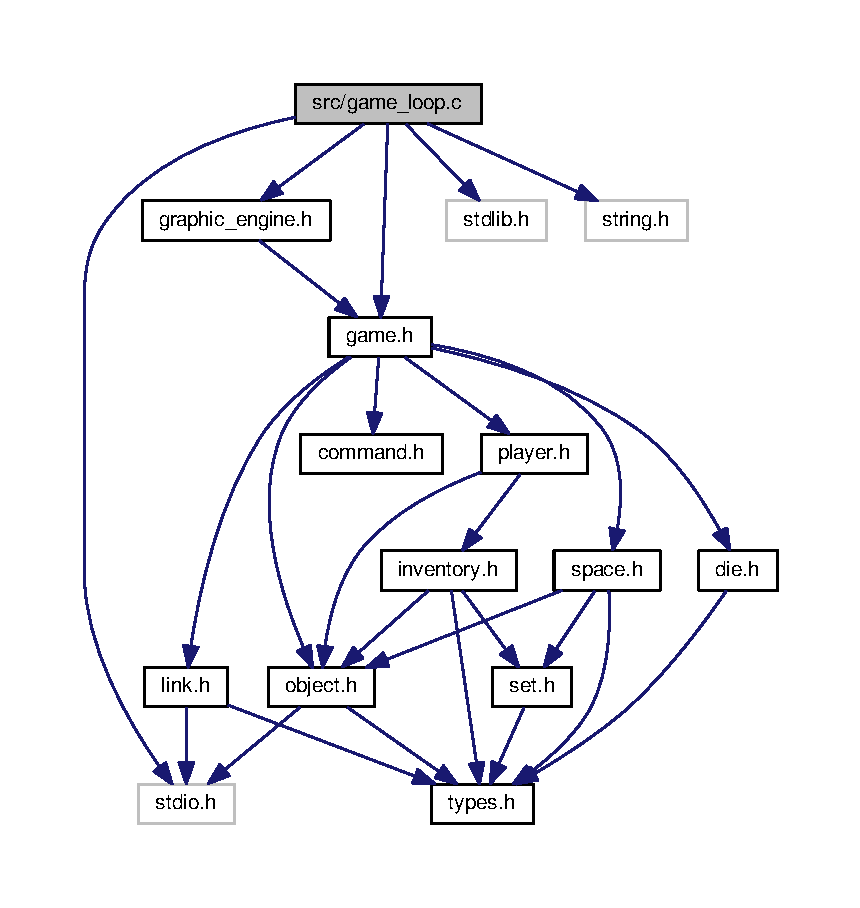
\includegraphics[width=350pt]{game__loop_8c__incl}
\end{center}
\end{figure}
\subsection*{Functions}
\begin{DoxyCompactItemize}
\item 
int \hyperlink{game__loop_8c_a0ddf1224851353fc92bfbff6f499fa97}{main} (int argc, char $\ast$argv\mbox{[}$\,$\mbox{]})
\begin{DoxyCompactList}\small\item\em main function of game \end{DoxyCompactList}\end{DoxyCompactItemize}


\subsection{Detailed Description}
initializes the game 

It defines the game loop and contains the M\+A\+IN function for all the program

\begin{DoxyAuthor}{Author}
Juan Moreno 
\end{DoxyAuthor}
\begin{DoxyVersion}{Version}
3.\+0 
\end{DoxyVersion}
\begin{DoxyDate}{Date}
07-\/04-\/2018 
\end{DoxyDate}


\subsection{Function Documentation}
\index{game\+\_\+loop.\+c@{game\+\_\+loop.\+c}!main@{main}}
\index{main@{main}!game\+\_\+loop.\+c@{game\+\_\+loop.\+c}}
\subsubsection[{\texorpdfstring{main(int argc, char $\ast$argv[])}{main(int argc, char *argv[])}}]{\setlength{\rightskip}{0pt plus 5cm}int main (
\begin{DoxyParamCaption}
\item[{int}]{argc, }
\item[{char $\ast$}]{argv\mbox{[}$\,$\mbox{]}}
\end{DoxyParamCaption}
)}\hypertarget{game__loop_8c_a0ddf1224851353fc92bfbff6f499fa97}{}\label{game__loop_8c_a0ddf1224851353fc92bfbff6f499fa97}


main function of game 

This function is in charge of loading the main function of the game, it has everything working in order to do it properly.

\begin{DoxyAuthor}{Author}
Juan Moreno 
\end{DoxyAuthor}

\begin{DoxyParams}{Parameters}
{\em argc} & int. \\
\hline
{\em argv} & int. \\
\hline
\end{DoxyParams}
\begin{DoxyReturn}{Returns}
int value. 
\end{DoxyReturn}

\hypertarget{GameManagement_8c}{}\section{src/\+Game\+Management.c File Reference}
\label{GameManagement_8c}\index{src/\+Game\+Management.\+c@{src/\+Game\+Management.\+c}}


Contains the function that loads spaces.  


{\ttfamily \#include $<$stdio.\+h$>$}\\*
{\ttfamily \#include $<$stdlib.\+h$>$}\\*
{\ttfamily \#include $<$string.\+h$>$}\\*
{\ttfamily \#include \char`\"{}types.\+h\char`\"{}}\\*
{\ttfamily \#include \char`\"{}game.\+h\char`\"{}}\\*
{\ttfamily \#include \char`\"{}Game\+Management.\+h\char`\"{}}\\*
{\ttfamily \#include \char`\"{}link.\+h\char`\"{}}\\*
Include dependency graph for Game\+Management.\+c\+:
\nopagebreak
\begin{figure}[H]
\begin{center}
\leavevmode
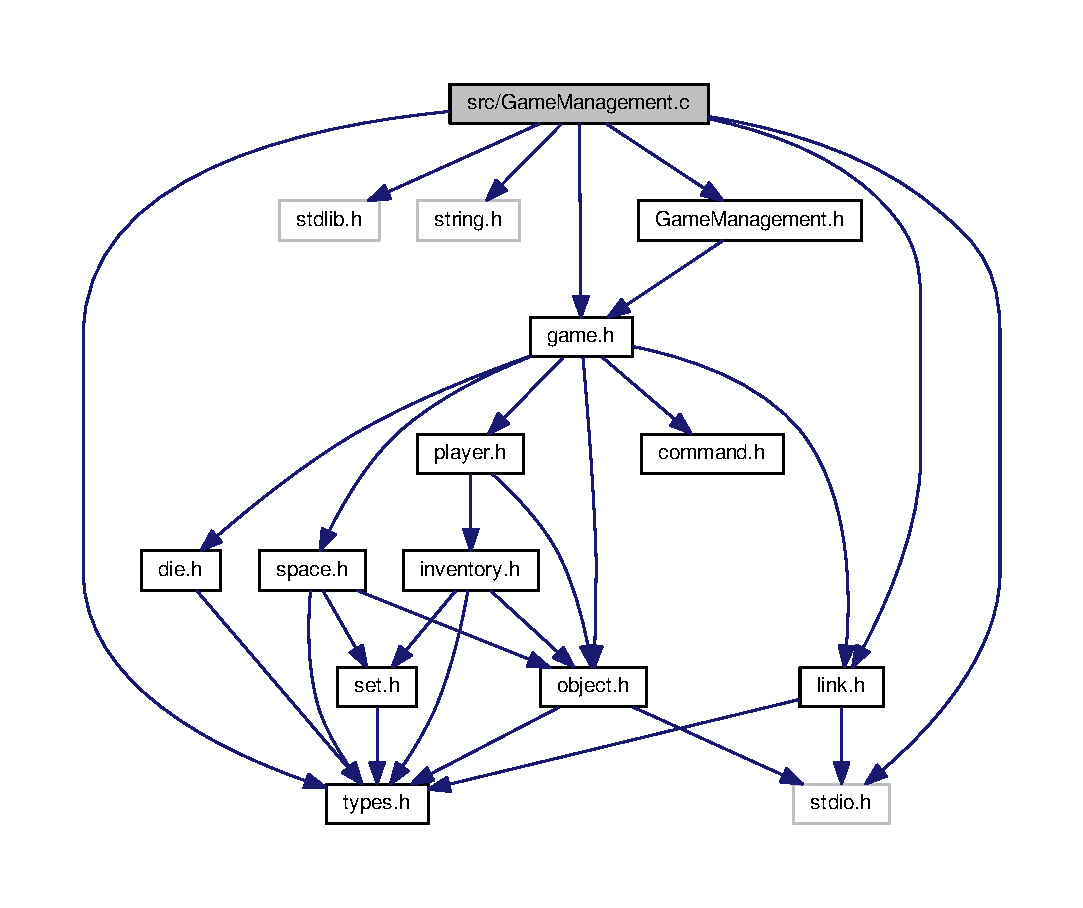
\includegraphics[width=350pt]{GameManagement_8c__incl}
\end{center}
\end{figure}
\subsection*{Functions}
\begin{DoxyCompactItemize}
\item 
\hyperlink{types_8h_a32c27cc471df37f4fc818d65de0a56c4}{S\+T\+A\+T\+US} \hyperlink{GameManagement_8c_a17503aa3d2345dc2f670ae0995ee9d81}{game\+\_\+management\+\_\+load\+\_\+graphics} (\hyperlink{space_8h_a67533ffc2b70463baecc38fb0629bbfc}{Space} $\ast$s, char $\ast$filename, \hyperlink{types_8h_a845e604fb28f7e3d97549da3448149d3}{Id} id)
\begin{DoxyCompactList}\small\item\em loads the graphics \end{DoxyCompactList}\item 
\hyperlink{types_8h_a32c27cc471df37f4fc818d65de0a56c4}{S\+T\+A\+T\+US} \hyperlink{GameManagement_8c_a51753ca919dffdc97f2249bd5edc4fa5}{game\+\_\+management\+\_\+load\+\_\+spaces} (\hyperlink{game_8h_a57156d39c530aec3fba3a9dad8c2dc6a}{Game} $\ast$game, char $\ast$filename)
\begin{DoxyCompactList}\small\item\em loads the spaces \end{DoxyCompactList}\item 
\hyperlink{types_8h_a32c27cc471df37f4fc818d65de0a56c4}{S\+T\+A\+T\+US} \hyperlink{GameManagement_8c_a59fad5fbf3d2f209ff5ab55060ad6974}{game\+\_\+management\+\_\+load\+\_\+objects} (\hyperlink{game_8h_a57156d39c530aec3fba3a9dad8c2dc6a}{Game} $\ast$game, char $\ast$filename)
\begin{DoxyCompactList}\small\item\em loads the objects \end{DoxyCompactList}\item 
\hyperlink{types_8h_a32c27cc471df37f4fc818d65de0a56c4}{S\+T\+A\+T\+US} \hyperlink{GameManagement_8c_a784e0d137d6ffdade3b65165be3a24bc}{game\+\_\+management\+\_\+load\+\_\+links} (\hyperlink{game_8h_a57156d39c530aec3fba3a9dad8c2dc6a}{Game} $\ast$game, char $\ast$filename)
\begin{DoxyCompactList}\small\item\em loads the links \end{DoxyCompactList}\item 
\hyperlink{types_8h_a32c27cc471df37f4fc818d65de0a56c4}{S\+T\+A\+T\+US} \hyperlink{GameManagement_8c_a7deb885075e008a0f2637330ce753047}{game\+\_\+management\+\_\+save\+\_\+game} (\hyperlink{game_8h_a57156d39c530aec3fba3a9dad8c2dc6a}{Game} $\ast$game, char $\ast$filename)
\begin{DoxyCompactList}\small\item\em saves the game \end{DoxyCompactList}\item 
\hyperlink{types_8h_a32c27cc471df37f4fc818d65de0a56c4}{S\+T\+A\+T\+US} \hyperlink{GameManagement_8c_afc72ef5dcc7b540e92ce2bec4fc0c466}{game\+\_\+management\+\_\+load\+\_\+game} (\hyperlink{game_8h_a57156d39c530aec3fba3a9dad8c2dc6a}{Game} $\ast$game, char $\ast$filename)
\begin{DoxyCompactList}\small\item\em saves the game \end{DoxyCompactList}\end{DoxyCompactItemize}


\subsection{Detailed Description}
Contains the function that loads spaces. 

The file is in charge of loading the structural part of the game such as the spaces, the objects and the links.

\begin{DoxyAuthor}{Author}
Borja Pérez 
\end{DoxyAuthor}
\begin{DoxyVersion}{Version}
3.\+0 
\end{DoxyVersion}
\begin{DoxyDate}{Date}
29-\/04-\/2018 
\end{DoxyDate}


\subsection{Function Documentation}
\index{Game\+Management.\+c@{Game\+Management.\+c}!game\+\_\+management\+\_\+load\+\_\+game@{game\+\_\+management\+\_\+load\+\_\+game}}
\index{game\+\_\+management\+\_\+load\+\_\+game@{game\+\_\+management\+\_\+load\+\_\+game}!Game\+Management.\+c@{Game\+Management.\+c}}
\subsubsection[{\texorpdfstring{game\+\_\+management\+\_\+load\+\_\+game(\+Game $\ast$game, char $\ast$filename)}{game_management_load_game(Game *game, char *filename)}}]{\setlength{\rightskip}{0pt plus 5cm}{\bf S\+T\+A\+T\+US} game\+\_\+management\+\_\+load\+\_\+game (
\begin{DoxyParamCaption}
\item[{{\bf Game} $\ast$}]{game, }
\item[{char $\ast$}]{filename}
\end{DoxyParamCaption}
)}\hypertarget{GameManagement_8c_afc72ef5dcc7b540e92ce2bec4fc0c466}{}\label{GameManagement_8c_afc72ef5dcc7b540e92ce2bec4fc0c466}


saves the game 

Function used to load the currect game positioning of objects, spaces, etc. and loads a new file

\begin{DoxyAuthor}{Author}
Borja Pérez 
\end{DoxyAuthor}

\begin{DoxyParams}{Parameters}
{\em game} & a pointer to the game. \\
\hline
{\em filename} & a string with the name of the file from where the game is load. \\
\hline
\end{DoxyParams}
\begin{DoxyReturn}{Returns}
S\+T\+A\+T\+US, E\+R\+R\+OR if argument received is N\+U\+LL, if not, OK. 
\end{DoxyReturn}
\index{Game\+Management.\+c@{Game\+Management.\+c}!game\+\_\+management\+\_\+load\+\_\+graphics@{game\+\_\+management\+\_\+load\+\_\+graphics}}
\index{game\+\_\+management\+\_\+load\+\_\+graphics@{game\+\_\+management\+\_\+load\+\_\+graphics}!Game\+Management.\+c@{Game\+Management.\+c}}
\subsubsection[{\texorpdfstring{game\+\_\+management\+\_\+load\+\_\+graphics(\+Space $\ast$s, char $\ast$filename, Id id)}{game_management_load_graphics(Space *s, char *filename, Id id)}}]{\setlength{\rightskip}{0pt plus 5cm}{\bf S\+T\+A\+T\+US} game\+\_\+management\+\_\+load\+\_\+graphics (
\begin{DoxyParamCaption}
\item[{{\bf Space} $\ast$}]{s, }
\item[{char $\ast$}]{filename, }
\item[{{\bf Id}}]{id}
\end{DoxyParamCaption}
)}\hypertarget{GameManagement_8c_a17503aa3d2345dc2f670ae0995ee9d81}{}\label{GameManagement_8c_a17503aa3d2345dc2f670ae0995ee9d81}


loads the graphics 

Detects graphics in a file (P.\+E graphics.\+txt) and loads them into a game.

\begin{DoxyAuthor}{Author}
Borja Pérez 
\end{DoxyAuthor}

\begin{DoxyParams}{Parameters}
{\em s} & a pointer to the space where the graphics will be loaded. \\
\hline
{\em filename} & a string with the name of the file in where the spaces are loaded. \\
\hline
{\em id} & long int \\
\hline
\end{DoxyParams}
\begin{DoxyReturn}{Returns}
S\+T\+A\+T\+US, E\+R\+R\+OR if argument received is N\+U\+LL, if not, OK. 
\end{DoxyReturn}
\index{Game\+Management.\+c@{Game\+Management.\+c}!game\+\_\+management\+\_\+load\+\_\+links@{game\+\_\+management\+\_\+load\+\_\+links}}
\index{game\+\_\+management\+\_\+load\+\_\+links@{game\+\_\+management\+\_\+load\+\_\+links}!Game\+Management.\+c@{Game\+Management.\+c}}
\subsubsection[{\texorpdfstring{game\+\_\+management\+\_\+load\+\_\+links(\+Game $\ast$game, char $\ast$filename)}{game_management_load_links(Game *game, char *filename)}}]{\setlength{\rightskip}{0pt plus 5cm}{\bf S\+T\+A\+T\+US} game\+\_\+management\+\_\+load\+\_\+links (
\begin{DoxyParamCaption}
\item[{{\bf Game} $\ast$}]{game, }
\item[{char $\ast$}]{filename}
\end{DoxyParamCaption}
)}\hypertarget{GameManagement_8c_a784e0d137d6ffdade3b65165be3a24bc}{}\label{GameManagement_8c_a784e0d137d6ffdade3b65165be3a24bc}


loads the links 

Detects links in a file (P.\+E. data.\+dat) and loads them into a game

\begin{DoxyAuthor}{Author}
Borja Pérez 
\end{DoxyAuthor}

\begin{DoxyParams}{Parameters}
{\em game} & a pointer to the game where the links will be loaded. \\
\hline
{\em filename} & a string with the name of the file in where the links are saved. \\
\hline
\end{DoxyParams}
\begin{DoxyReturn}{Returns}
S\+T\+A\+T\+US, E\+R\+R\+OR if argument received is N\+U\+LL, if not, OK. 
\end{DoxyReturn}
\index{Game\+Management.\+c@{Game\+Management.\+c}!game\+\_\+management\+\_\+load\+\_\+objects@{game\+\_\+management\+\_\+load\+\_\+objects}}
\index{game\+\_\+management\+\_\+load\+\_\+objects@{game\+\_\+management\+\_\+load\+\_\+objects}!Game\+Management.\+c@{Game\+Management.\+c}}
\subsubsection[{\texorpdfstring{game\+\_\+management\+\_\+load\+\_\+objects(\+Game $\ast$game, char $\ast$filename)}{game_management_load_objects(Game *game, char *filename)}}]{\setlength{\rightskip}{0pt plus 5cm}{\bf S\+T\+A\+T\+US} game\+\_\+management\+\_\+load\+\_\+objects (
\begin{DoxyParamCaption}
\item[{{\bf Game} $\ast$}]{game, }
\item[{char $\ast$}]{filename}
\end{DoxyParamCaption}
)}\hypertarget{GameManagement_8c_a59fad5fbf3d2f209ff5ab55060ad6974}{}\label{GameManagement_8c_a59fad5fbf3d2f209ff5ab55060ad6974}


loads the objects 

Detects objects in a file (P.\+E. data.\+dat) and loads them into a game

\begin{DoxyAuthor}{Author}
Borja Pérez 
\end{DoxyAuthor}

\begin{DoxyParams}{Parameters}
{\em game} & a pointer to the game where the objects will be loaded. \\
\hline
{\em filename} & a string with the name of the file in where the objects are saved. \\
\hline
\end{DoxyParams}
\begin{DoxyReturn}{Returns}
S\+T\+A\+T\+US, E\+R\+R\+OR if argument received is N\+U\+LL, if not, OK. 
\end{DoxyReturn}
\index{Game\+Management.\+c@{Game\+Management.\+c}!game\+\_\+management\+\_\+load\+\_\+spaces@{game\+\_\+management\+\_\+load\+\_\+spaces}}
\index{game\+\_\+management\+\_\+load\+\_\+spaces@{game\+\_\+management\+\_\+load\+\_\+spaces}!Game\+Management.\+c@{Game\+Management.\+c}}
\subsubsection[{\texorpdfstring{game\+\_\+management\+\_\+load\+\_\+spaces(\+Game $\ast$game, char $\ast$filename)}{game_management_load_spaces(Game *game, char *filename)}}]{\setlength{\rightskip}{0pt plus 5cm}{\bf S\+T\+A\+T\+US} game\+\_\+management\+\_\+load\+\_\+spaces (
\begin{DoxyParamCaption}
\item[{{\bf Game} $\ast$}]{game, }
\item[{char $\ast$}]{filename}
\end{DoxyParamCaption}
)}\hypertarget{GameManagement_8c_a51753ca919dffdc97f2249bd5edc4fa5}{}\label{GameManagement_8c_a51753ca919dffdc97f2249bd5edc4fa5}


loads the spaces 

Detects spaces in a file (P.\+E. data.\+dat) and loads them into a game.

\begin{DoxyAuthor}{Author}
Borja Pérez 
\end{DoxyAuthor}

\begin{DoxyParams}{Parameters}
{\em game} & a pointer to the game where the spaces will be loaded. \\
\hline
{\em filename} & a string with the name of the file in where the spaces are saved. \\
\hline
\end{DoxyParams}
\begin{DoxyReturn}{Returns}
S\+T\+A\+T\+US, E\+R\+R\+OR if argument received is N\+U\+LL, if not, OK. 
\end{DoxyReturn}
\index{Game\+Management.\+c@{Game\+Management.\+c}!game\+\_\+management\+\_\+save\+\_\+game@{game\+\_\+management\+\_\+save\+\_\+game}}
\index{game\+\_\+management\+\_\+save\+\_\+game@{game\+\_\+management\+\_\+save\+\_\+game}!Game\+Management.\+c@{Game\+Management.\+c}}
\subsubsection[{\texorpdfstring{game\+\_\+management\+\_\+save\+\_\+game(\+Game $\ast$game, char $\ast$filename)}{game_management_save_game(Game *game, char *filename)}}]{\setlength{\rightskip}{0pt plus 5cm}{\bf S\+T\+A\+T\+US} game\+\_\+management\+\_\+save\+\_\+game (
\begin{DoxyParamCaption}
\item[{{\bf Game} $\ast$}]{game, }
\item[{char $\ast$}]{filename}
\end{DoxyParamCaption}
)}\hypertarget{GameManagement_8c_a7deb885075e008a0f2637330ce753047}{}\label{GameManagement_8c_a7deb885075e008a0f2637330ce753047}


saves the game 

Function used to save the currect game positioning of objects, spaces, etc. and creates a new file

\begin{DoxyAuthor}{Author}
Borja Pérez 
\end{DoxyAuthor}

\begin{DoxyParams}{Parameters}
{\em game} & a pointer to the game. \\
\hline
{\em filename} & a string with the name of the file in where the game is saved. \\
\hline
\end{DoxyParams}
\begin{DoxyReturn}{Returns}
S\+T\+A\+T\+US, E\+R\+R\+OR if argument received is N\+U\+LL, if not, OK. 
\end{DoxyReturn}

\hypertarget{graphic__engine_8c}{}\section{src/graphic\+\_\+engine.c File Reference}
\label{graphic__engine_8c}\index{src/graphic\+\_\+engine.\+c@{src/graphic\+\_\+engine.\+c}}


defines the graphic engine  


{\ttfamily \#include $<$stdlib.\+h$>$}\\*
{\ttfamily \#include $<$stdio.\+h$>$}\\*
{\ttfamily \#include $<$string.\+h$>$}\\*
{\ttfamily \#include \char`\"{}screen.\+h\char`\"{}}\\*
{\ttfamily \#include \char`\"{}graphic\+\_\+engine.\+h\char`\"{}}\\*
{\ttfamily \#include \char`\"{}game.\+h\char`\"{}}\\*
Include dependency graph for graphic\+\_\+engine.\+c\+:
\nopagebreak
\begin{figure}[H]
\begin{center}
\leavevmode
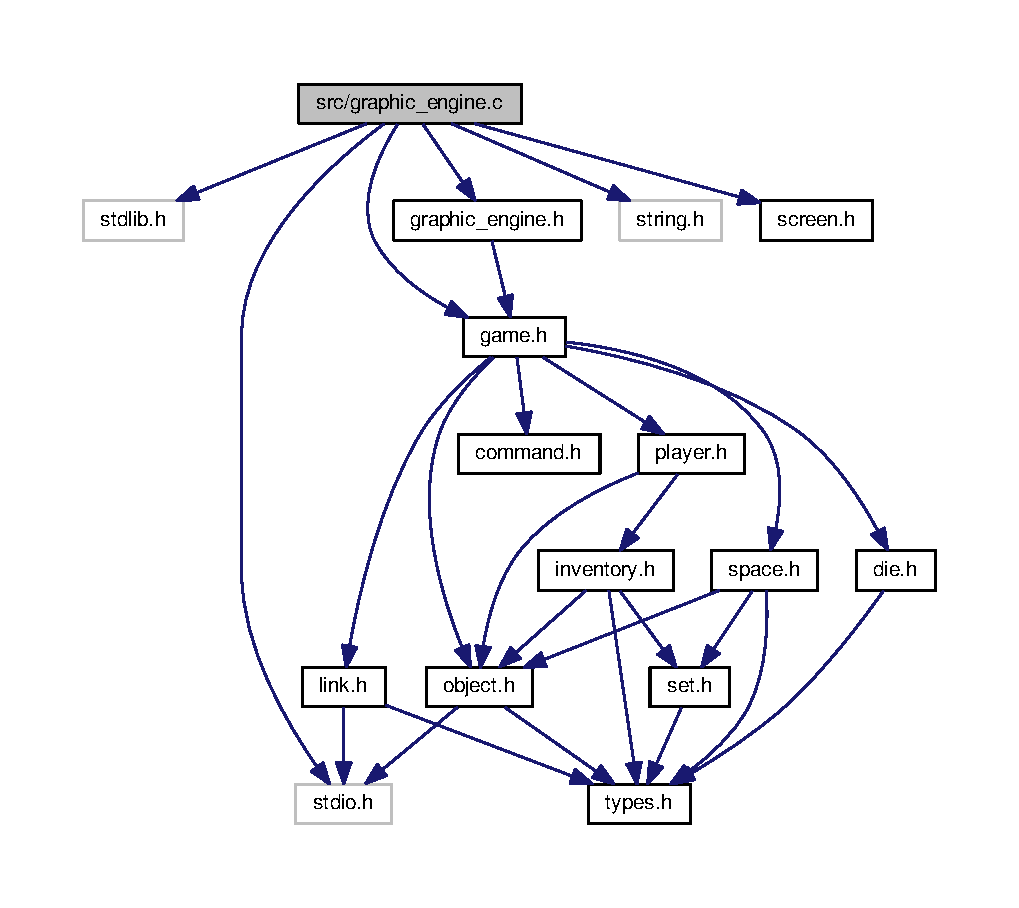
\includegraphics[width=350pt]{graphic__engine_8c__incl}
\end{center}
\end{figure}
\subsection*{Data Structures}
\begin{DoxyCompactItemize}
\item 
struct \hyperlink{struct__Graphic__engine}{\+\_\+\+Graphic\+\_\+engine}
\begin{DoxyCompactList}\small\item\em graphic design \end{DoxyCompactList}\end{DoxyCompactItemize}
\subsection*{Macros}
\begin{DoxyCompactItemize}
\item 
\#define \hyperlink{graphic__engine_8c_a285e2a8573a9f65f505d752acacc6d2c}{S\+S\+I\+ZE}~11
\end{DoxyCompactItemize}
\subsection*{Functions}
\begin{DoxyCompactItemize}
\item 
\hyperlink{graphic__engine_8h_ae1bc5cdbfce93098f066274fdea49af1}{Graphic\+\_\+engine} $\ast$ \hyperlink{graphic__engine_8c_a8c3d9abe7282bee1d77d23ea80a4bdec}{graphic\+\_\+engine\+\_\+create} ()
\begin{DoxyCompactList}\small\item\em creates the graphic engine \end{DoxyCompactList}\item 
void \hyperlink{graphic__engine_8c_a5a5eac4ef2033c5ad71aa6895f362f79}{graphic\+\_\+engine\+\_\+destroy} (\hyperlink{graphic__engine_8h_ae1bc5cdbfce93098f066274fdea49af1}{Graphic\+\_\+engine} $\ast$ge)
\begin{DoxyCompactList}\small\item\em frees memory \end{DoxyCompactList}\item 
void \hyperlink{graphic__engine_8c_a0e275aa477d5fa59e903da33a2a40a5d}{graphic\+\_\+engine\+\_\+paint\+\_\+game} (\hyperlink{graphic__engine_8h_ae1bc5cdbfce93098f066274fdea49af1}{Graphic\+\_\+engine} $\ast$ge, \hyperlink{game_8h_a57156d39c530aec3fba3a9dad8c2dc6a}{Game} $\ast$game)
\begin{DoxyCompactList}\small\item\em paints the game \end{DoxyCompactList}\end{DoxyCompactItemize}


\subsection{Detailed Description}
defines the graphic engine 

Module that contains the graphic information of the game, it is in charge of printing everything.

\begin{DoxyAuthor}{Author}
Dan Roife 
\end{DoxyAuthor}
\begin{DoxyVersion}{Version}
1.\+2 
\end{DoxyVersion}
\begin{DoxyDate}{Date}
07-\/04-\/2018 
\end{DoxyDate}


\subsection{Macro Definition Documentation}
\index{graphic\+\_\+engine.\+c@{graphic\+\_\+engine.\+c}!S\+S\+I\+ZE@{S\+S\+I\+ZE}}
\index{S\+S\+I\+ZE@{S\+S\+I\+ZE}!graphic\+\_\+engine.\+c@{graphic\+\_\+engine.\+c}}
\subsubsection[{\texorpdfstring{S\+S\+I\+ZE}{SSIZE}}]{\setlength{\rightskip}{0pt plus 5cm}\#define S\+S\+I\+ZE~11}\hypertarget{graphic__engine_8c_a285e2a8573a9f65f505d752acacc6d2c}{}\label{graphic__engine_8c_a285e2a8573a9f65f505d752acacc6d2c}
maximum size 

\subsection{Function Documentation}
\index{graphic\+\_\+engine.\+c@{graphic\+\_\+engine.\+c}!graphic\+\_\+engine\+\_\+create@{graphic\+\_\+engine\+\_\+create}}
\index{graphic\+\_\+engine\+\_\+create@{graphic\+\_\+engine\+\_\+create}!graphic\+\_\+engine.\+c@{graphic\+\_\+engine.\+c}}
\subsubsection[{\texorpdfstring{graphic\+\_\+engine\+\_\+create()}{graphic_engine_create()}}]{\setlength{\rightskip}{0pt plus 5cm}{\bf Graphic\+\_\+engine}$\ast$ graphic\+\_\+engine\+\_\+create (
\begin{DoxyParamCaption}
{}
\end{DoxyParamCaption}
)}\hypertarget{graphic__engine_8c_a8c3d9abe7282bee1d77d23ea80a4bdec}{}\label{graphic__engine_8c_a8c3d9abe7282bee1d77d23ea80a4bdec}


creates the graphic engine 

Allocates the memory for a new graphic engine and declares its parts

\begin{DoxyAuthor}{Author}
Dan Roife 
\end{DoxyAuthor}
\begin{DoxyReturn}{Returns}
pointer to a graphic engine. 
\end{DoxyReturn}
\index{graphic\+\_\+engine.\+c@{graphic\+\_\+engine.\+c}!graphic\+\_\+engine\+\_\+destroy@{graphic\+\_\+engine\+\_\+destroy}}
\index{graphic\+\_\+engine\+\_\+destroy@{graphic\+\_\+engine\+\_\+destroy}!graphic\+\_\+engine.\+c@{graphic\+\_\+engine.\+c}}
\subsubsection[{\texorpdfstring{graphic\+\_\+engine\+\_\+destroy(\+Graphic\+\_\+engine $\ast$ge)}{graphic_engine_destroy(Graphic_engine *ge)}}]{\setlength{\rightskip}{0pt plus 5cm}void graphic\+\_\+engine\+\_\+destroy (
\begin{DoxyParamCaption}
\item[{{\bf Graphic\+\_\+engine} $\ast$}]{ge}
\end{DoxyParamCaption}
)}\hypertarget{graphic__engine_8c_a5a5eac4ef2033c5ad71aa6895f362f79}{}\label{graphic__engine_8c_a5a5eac4ef2033c5ad71aa6895f362f79}


frees memory 

Frees the memory allocated for the graphic engine and its parts.

\begin{DoxyAuthor}{Author}
Dan Roife 
\end{DoxyAuthor}

\begin{DoxyParams}{Parameters}
{\em ge} & pointer to graphic engine. \\
\hline
\end{DoxyParams}
\begin{DoxyReturn}{Returns}
void function. 
\end{DoxyReturn}
\index{graphic\+\_\+engine.\+c@{graphic\+\_\+engine.\+c}!graphic\+\_\+engine\+\_\+paint\+\_\+game@{graphic\+\_\+engine\+\_\+paint\+\_\+game}}
\index{graphic\+\_\+engine\+\_\+paint\+\_\+game@{graphic\+\_\+engine\+\_\+paint\+\_\+game}!graphic\+\_\+engine.\+c@{graphic\+\_\+engine.\+c}}
\subsubsection[{\texorpdfstring{graphic\+\_\+engine\+\_\+paint\+\_\+game(\+Graphic\+\_\+engine $\ast$ge, Game $\ast$game)}{graphic_engine_paint_game(Graphic_engine *ge, Game *game)}}]{\setlength{\rightskip}{0pt plus 5cm}void graphic\+\_\+engine\+\_\+paint\+\_\+game (
\begin{DoxyParamCaption}
\item[{{\bf Graphic\+\_\+engine} $\ast$}]{ge, }
\item[{{\bf Game} $\ast$}]{game}
\end{DoxyParamCaption}
)}\hypertarget{graphic__engine_8c_a0e275aa477d5fa59e903da33a2a40a5d}{}\label{graphic__engine_8c_a0e275aa477d5fa59e903da33a2a40a5d}


paints the game 

Shows a graphic interface with the contents of the game.

\begin{DoxyAuthor}{Author}
Dan Roife 
\end{DoxyAuthor}

\begin{DoxyParams}{Parameters}
{\em ge} & pointer to graphic engine. \\
\hline
{\em game} & pointer to game. \\
\hline
\end{DoxyParams}
\begin{DoxyReturn}{Returns}
void function. 
\end{DoxyReturn}

\hypertarget{inventory__test_8c}{}\section{src/inventory\+\_\+test.c File Reference}
\label{inventory__test_8c}\index{src/inventory\+\_\+test.\+c@{src/inventory\+\_\+test.\+c}}


It tests inventory module.  


{\ttfamily \#include $<$stdio.\+h$>$}\\*
{\ttfamily \#include $<$stdlib.\+h$>$}\\*
{\ttfamily \#include $<$string.\+h$>$}\\*
{\ttfamily \#include \char`\"{}inventory.\+h\char`\"{}}\\*
{\ttfamily \#include \char`\"{}inventory\+\_\+test.\+h\char`\"{}}\\*
{\ttfamily \#include \char`\"{}test.\+h\char`\"{}}\\*
{\ttfamily \#include \char`\"{}set.\+h\char`\"{}}\\*
Include dependency graph for inventory\+\_\+test.\+c\+:
\nopagebreak
\begin{figure}[H]
\begin{center}
\leavevmode
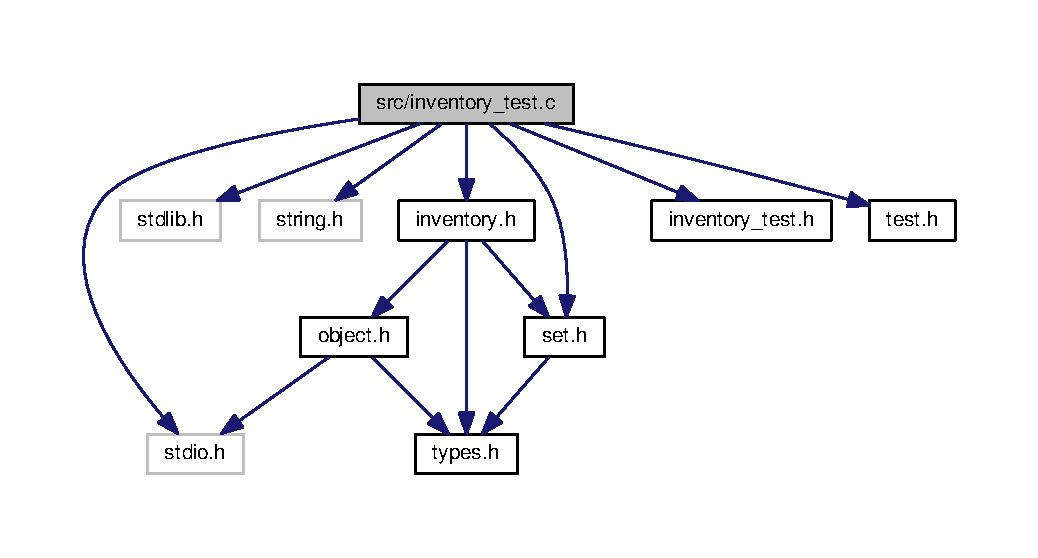
\includegraphics[width=350pt]{inventory__test_8c__incl}
\end{center}
\end{figure}
\subsection*{Macros}
\begin{DoxyCompactItemize}
\item 
\#define \hyperlink{inventory__test_8c_a2a77d2f2c5b698c69c19e1f8782bf709}{M\+A\+X\+\_\+\+T\+E\+S\+TS}~21
\end{DoxyCompactItemize}
\subsection*{Functions}
\begin{DoxyCompactItemize}
\item 
int \hyperlink{inventory__test_8c_a3c04138a5bfe5d72780bb7e82a18e627}{main} (int argc, char $\ast$$\ast$argv)
\begin{DoxyCompactList}\small\item\em Main function for inventory unit tests. \end{DoxyCompactList}\item 
void \hyperlink{inventory__test_8c_a33638f1a88ae16ab8d6bee00145b82b8}{test1\+\_\+inventory\+\_\+create} ()
\item 
void \hyperlink{inventory__test_8c_a40a21fc4411716ecfa2bbb33c783df94}{test1\+\_\+inventory\+\_\+add\+\_\+id} ()
\item 
void \hyperlink{inventory__test_8c_abfb3407529398f76999549e42d567a7e}{test2\+\_\+inventory\+\_\+add\+\_\+id} ()
\item 
void \hyperlink{inventory__test_8c_adb75e7f71748feea51900c782343f550}{test3\+\_\+inventory\+\_\+add\+\_\+id} ()
\item 
void \hyperlink{inventory__test_8c_a967d37c163cbf8ea9335b506c1713f4a}{test4\+\_\+inventory\+\_\+add\+\_\+id} ()
\item 
void \hyperlink{inventory__test_8c_a8e69ae5a26b0115971e51ab94616fb85}{test5\+\_\+inventory\+\_\+add\+\_\+id} ()
\item 
void \hyperlink{inventory__test_8c_ac38fe4f7cdf9fa3972e975ee07caf876}{test1\+\_\+inventory\+\_\+get\+\_\+set} ()
\item 
void \hyperlink{inventory__test_8c_a66737b763a088f8a85549e846b01fbdb}{test2\+\_\+inventory\+\_\+get\+\_\+set} ()
\item 
void \hyperlink{inventory__test_8c_a30d80ddf084113e14192c7a5031528c5}{test1\+\_\+inventory\+\_\+delete\+\_\+id} ()
\item 
void \hyperlink{inventory__test_8c_a23c8b0ed664f86b5fdafbfbd875ee27d}{test2\+\_\+inventory\+\_\+delete\+\_\+id} ()
\item 
void \hyperlink{inventory__test_8c_a3dc930ea10c0e538e9f7227d5a7cdfa1}{test3\+\_\+inventory\+\_\+delete\+\_\+id} ()
\item 
void \hyperlink{inventory__test_8c_ab161eafe6a61db39b2237e97c677d822}{test1\+\_\+inventory\+\_\+destroy} ()
\item 
void \hyperlink{inventory__test_8c_a9f3daec28c696c0671e6a3e905359741}{test2\+\_\+inventory\+\_\+destroy} ()
\item 
void \hyperlink{inventory__test_8c_a7229ceb1916b0da955d23598da89d5ea}{test1\+\_\+inventory\+\_\+print} ()
\item 
void \hyperlink{inventory__test_8c_a76718582c0fbf43fbfc9e6bf3264f48e}{test1\+\_\+inventory\+\_\+get\+\_\+object} ()
\item 
void \hyperlink{inventory__test_8c_a6a440546c4b5335db5bb0e93688bf847}{test2\+\_\+inventory\+\_\+get\+\_\+object} ()
\item 
void \hyperlink{inventory__test_8c_afe8c9730e30b58535afc0481970ab2b1}{test1\+\_\+inventory\+\_\+is\+\_\+empty} ()
\item 
void \hyperlink{inventory__test_8c_a4d2a2a4d4ba59446d013debfe9bf05dc}{test2\+\_\+inventory\+\_\+is\+\_\+empty} ()
\item 
void \hyperlink{inventory__test_8c_a9c8daeb141dbec6ddd5621edade53091}{test3\+\_\+inventory\+\_\+is\+\_\+empty} ()
\item 
void \hyperlink{inventory__test_8c_a7eb3ba387e33c42ff45331c9d9aada34}{test1\+\_\+inventory\+\_\+is\+\_\+full} ()
\item 
void \hyperlink{inventory__test_8c_a1c9e567d4919d5aaccc9580815a8a81d}{test2\+\_\+inventory\+\_\+is\+\_\+full} ()
\end{DoxyCompactItemize}


\subsection{Detailed Description}
It tests inventory module. 

\begin{DoxyAuthor}{Author}
Andres Mena 
\end{DoxyAuthor}
\begin{DoxyVersion}{Version}
1.\+0 
\end{DoxyVersion}
\begin{DoxyDate}{Date}
31-\/03-\/2018 
\end{DoxyDate}
\begin{DoxyCopyright}{Copyright}
G\+NU Public License 
\end{DoxyCopyright}


\subsection{Macro Definition Documentation}
\index{inventory\+\_\+test.\+c@{inventory\+\_\+test.\+c}!M\+A\+X\+\_\+\+T\+E\+S\+TS@{M\+A\+X\+\_\+\+T\+E\+S\+TS}}
\index{M\+A\+X\+\_\+\+T\+E\+S\+TS@{M\+A\+X\+\_\+\+T\+E\+S\+TS}!inventory\+\_\+test.\+c@{inventory\+\_\+test.\+c}}
\subsubsection[{\texorpdfstring{M\+A\+X\+\_\+\+T\+E\+S\+TS}{MAX_TESTS}}]{\setlength{\rightskip}{0pt plus 5cm}\#define M\+A\+X\+\_\+\+T\+E\+S\+TS~21}\hypertarget{inventory__test_8c_a2a77d2f2c5b698c69c19e1f8782bf709}{}\label{inventory__test_8c_a2a77d2f2c5b698c69c19e1f8782bf709}
Max amount of tests posible 

\subsection{Function Documentation}
\index{inventory\+\_\+test.\+c@{inventory\+\_\+test.\+c}!main@{main}}
\index{main@{main}!inventory\+\_\+test.\+c@{inventory\+\_\+test.\+c}}
\subsubsection[{\texorpdfstring{main(int argc, char $\ast$$\ast$argv)}{main(int argc, char **argv)}}]{\setlength{\rightskip}{0pt plus 5cm}int main (
\begin{DoxyParamCaption}
\item[{int}]{argc, }
\item[{char $\ast$$\ast$}]{argv}
\end{DoxyParamCaption}
)}\hypertarget{inventory__test_8c_a3c04138a5bfe5d72780bb7e82a18e627}{}\label{inventory__test_8c_a3c04138a5bfe5d72780bb7e82a18e627}


Main function for inventory unit tests. 

You may execute A\+LL or a S\+I\+N\+G\+LE test 1.-\/ No parameter -\/$>$ A\+LL test are executed 2.-\/ A number means a particular test (the one identified by that number) is executed \index{inventory\+\_\+test.\+c@{inventory\+\_\+test.\+c}!test1\+\_\+inventory\+\_\+add\+\_\+id@{test1\+\_\+inventory\+\_\+add\+\_\+id}}
\index{test1\+\_\+inventory\+\_\+add\+\_\+id@{test1\+\_\+inventory\+\_\+add\+\_\+id}!inventory\+\_\+test.\+c@{inventory\+\_\+test.\+c}}
\subsubsection[{\texorpdfstring{test1\+\_\+inventory\+\_\+add\+\_\+id()}{test1_inventory_add_id()}}]{\setlength{\rightskip}{0pt plus 5cm}void test1\+\_\+inventory\+\_\+add\+\_\+id (
\begin{DoxyParamCaption}
{}
\end{DoxyParamCaption}
)}\hypertarget{inventory__test_8c_a40a21fc4411716ecfa2bbb33c783df94}{}\label{inventory__test_8c_a40a21fc4411716ecfa2bbb33c783df94}
\begin{DoxyRefDesc}{Test}
\item[\hyperlink{test__test000002}{Test}]Test adding id to inventory \end{DoxyRefDesc}
\begin{DoxyPrecond}{Precondition}
N\+U\+LL pointer to inventory 
\end{DoxyPrecond}
\begin{DoxyPostcond}{Postcondition}
S\+T\+A\+T\+US == E\+R\+R\+OR 
\end{DoxyPostcond}
\index{inventory\+\_\+test.\+c@{inventory\+\_\+test.\+c}!test1\+\_\+inventory\+\_\+create@{test1\+\_\+inventory\+\_\+create}}
\index{test1\+\_\+inventory\+\_\+create@{test1\+\_\+inventory\+\_\+create}!inventory\+\_\+test.\+c@{inventory\+\_\+test.\+c}}
\subsubsection[{\texorpdfstring{test1\+\_\+inventory\+\_\+create()}{test1_inventory_create()}}]{\setlength{\rightskip}{0pt plus 5cm}void test1\+\_\+inventory\+\_\+create (
\begin{DoxyParamCaption}
{}
\end{DoxyParamCaption}
)}\hypertarget{inventory__test_8c_a33638f1a88ae16ab8d6bee00145b82b8}{}\label{inventory__test_8c_a33638f1a88ae16ab8d6bee00145b82b8}
\begin{DoxyRefDesc}{Test}
\item[\hyperlink{test__test000001}{Test}]Test inventory creation \end{DoxyRefDesc}
\begin{DoxyPrecond}{Precondition}
link ID 
\end{DoxyPrecond}
\begin{DoxyPostcond}{Postcondition}
Non N\+U\+LL pointer to inventory 
\end{DoxyPostcond}
\index{inventory\+\_\+test.\+c@{inventory\+\_\+test.\+c}!test1\+\_\+inventory\+\_\+delete\+\_\+id@{test1\+\_\+inventory\+\_\+delete\+\_\+id}}
\index{test1\+\_\+inventory\+\_\+delete\+\_\+id@{test1\+\_\+inventory\+\_\+delete\+\_\+id}!inventory\+\_\+test.\+c@{inventory\+\_\+test.\+c}}
\subsubsection[{\texorpdfstring{test1\+\_\+inventory\+\_\+delete\+\_\+id()}{test1_inventory_delete_id()}}]{\setlength{\rightskip}{0pt plus 5cm}void test1\+\_\+inventory\+\_\+delete\+\_\+id (
\begin{DoxyParamCaption}
{}
\end{DoxyParamCaption}
)}\hypertarget{inventory__test_8c_a30d80ddf084113e14192c7a5031528c5}{}\label{inventory__test_8c_a30d80ddf084113e14192c7a5031528c5}
\begin{DoxyRefDesc}{Test}
\item[\hyperlink{test__test000009}{Test}]Test deleting id from inventory \end{DoxyRefDesc}
\begin{DoxyPrecond}{Precondition}
N\+U\+LL pointer to inventory and N\+O\+\_\+\+ID 
\end{DoxyPrecond}
\begin{DoxyPostcond}{Postcondition}
E\+R\+R\+OR 
\end{DoxyPostcond}
\index{inventory\+\_\+test.\+c@{inventory\+\_\+test.\+c}!test1\+\_\+inventory\+\_\+destroy@{test1\+\_\+inventory\+\_\+destroy}}
\index{test1\+\_\+inventory\+\_\+destroy@{test1\+\_\+inventory\+\_\+destroy}!inventory\+\_\+test.\+c@{inventory\+\_\+test.\+c}}
\subsubsection[{\texorpdfstring{test1\+\_\+inventory\+\_\+destroy()}{test1_inventory_destroy()}}]{\setlength{\rightskip}{0pt plus 5cm}void test1\+\_\+inventory\+\_\+destroy (
\begin{DoxyParamCaption}
{}
\end{DoxyParamCaption}
)}\hypertarget{inventory__test_8c_ab161eafe6a61db39b2237e97c677d822}{}\label{inventory__test_8c_ab161eafe6a61db39b2237e97c677d822}
\begin{DoxyRefDesc}{Test}
\item[\hyperlink{test__test000012}{Test}]Test destroying inventory \end{DoxyRefDesc}
\begin{DoxyPrecond}{Precondition}
N\+U\+LL pointer to inventory 
\end{DoxyPrecond}
\begin{DoxyPostcond}{Postcondition}
E\+R\+R\+OR 
\end{DoxyPostcond}
\index{inventory\+\_\+test.\+c@{inventory\+\_\+test.\+c}!test1\+\_\+inventory\+\_\+get\+\_\+object@{test1\+\_\+inventory\+\_\+get\+\_\+object}}
\index{test1\+\_\+inventory\+\_\+get\+\_\+object@{test1\+\_\+inventory\+\_\+get\+\_\+object}!inventory\+\_\+test.\+c@{inventory\+\_\+test.\+c}}
\subsubsection[{\texorpdfstring{test1\+\_\+inventory\+\_\+get\+\_\+object()}{test1_inventory_get_object()}}]{\setlength{\rightskip}{0pt plus 5cm}void test1\+\_\+inventory\+\_\+get\+\_\+object (
\begin{DoxyParamCaption}
{}
\end{DoxyParamCaption}
)}\hypertarget{inventory__test_8c_a76718582c0fbf43fbfc9e6bf3264f48e}{}\label{inventory__test_8c_a76718582c0fbf43fbfc9e6bf3264f48e}
\begin{DoxyRefDesc}{Test}
\item[\hyperlink{test__test000020}{Test}]Test getting objects from inventory \end{DoxyRefDesc}
\begin{DoxyPrecond}{Precondition}
N\+U\+LL pointer to inventory 
\end{DoxyPrecond}
\begin{DoxyPostcond}{Postcondition}
N\+O\+\_\+\+ID 
\end{DoxyPostcond}
\index{inventory\+\_\+test.\+c@{inventory\+\_\+test.\+c}!test1\+\_\+inventory\+\_\+get\+\_\+set@{test1\+\_\+inventory\+\_\+get\+\_\+set}}
\index{test1\+\_\+inventory\+\_\+get\+\_\+set@{test1\+\_\+inventory\+\_\+get\+\_\+set}!inventory\+\_\+test.\+c@{inventory\+\_\+test.\+c}}
\subsubsection[{\texorpdfstring{test1\+\_\+inventory\+\_\+get\+\_\+set()}{test1_inventory_get_set()}}]{\setlength{\rightskip}{0pt plus 5cm}void test1\+\_\+inventory\+\_\+get\+\_\+set (
\begin{DoxyParamCaption}
{}
\end{DoxyParamCaption}
)}\hypertarget{inventory__test_8c_ac38fe4f7cdf9fa3972e975ee07caf876}{}\label{inventory__test_8c_ac38fe4f7cdf9fa3972e975ee07caf876}
\begin{DoxyRefDesc}{Test}
\item[\hyperlink{test__test000007}{Test}]Test getting set from inventory \end{DoxyRefDesc}
\begin{DoxyPrecond}{Precondition}
N\+U\+LL pointer to inventory 
\end{DoxyPrecond}
\begin{DoxyPostcond}{Postcondition}
N\+U\+LL set pointer 
\end{DoxyPostcond}
\index{inventory\+\_\+test.\+c@{inventory\+\_\+test.\+c}!test1\+\_\+inventory\+\_\+is\+\_\+empty@{test1\+\_\+inventory\+\_\+is\+\_\+empty}}
\index{test1\+\_\+inventory\+\_\+is\+\_\+empty@{test1\+\_\+inventory\+\_\+is\+\_\+empty}!inventory\+\_\+test.\+c@{inventory\+\_\+test.\+c}}
\subsubsection[{\texorpdfstring{test1\+\_\+inventory\+\_\+is\+\_\+empty()}{test1_inventory_is_empty()}}]{\setlength{\rightskip}{0pt plus 5cm}void test1\+\_\+inventory\+\_\+is\+\_\+empty (
\begin{DoxyParamCaption}
{}
\end{DoxyParamCaption}
)}\hypertarget{inventory__test_8c_afe8c9730e30b58535afc0481970ab2b1}{}\label{inventory__test_8c_afe8c9730e30b58535afc0481970ab2b1}
\begin{DoxyRefDesc}{Test}
\item[\hyperlink{test__test000017}{Test}]Test if inventory is empty \end{DoxyRefDesc}
\begin{DoxyPrecond}{Precondition}
N\+U\+LL Ponter to inventory 
\end{DoxyPrecond}
\begin{DoxyPostcond}{Postcondition}
B\+O\+OL == F\+A\+L\+SE 
\end{DoxyPostcond}
\index{inventory\+\_\+test.\+c@{inventory\+\_\+test.\+c}!test1\+\_\+inventory\+\_\+is\+\_\+full@{test1\+\_\+inventory\+\_\+is\+\_\+full}}
\index{test1\+\_\+inventory\+\_\+is\+\_\+full@{test1\+\_\+inventory\+\_\+is\+\_\+full}!inventory\+\_\+test.\+c@{inventory\+\_\+test.\+c}}
\subsubsection[{\texorpdfstring{test1\+\_\+inventory\+\_\+is\+\_\+full()}{test1_inventory_is_full()}}]{\setlength{\rightskip}{0pt plus 5cm}void test1\+\_\+inventory\+\_\+is\+\_\+full (
\begin{DoxyParamCaption}
{}
\end{DoxyParamCaption}
)}\hypertarget{inventory__test_8c_a7eb3ba387e33c42ff45331c9d9aada34}{}\label{inventory__test_8c_a7eb3ba387e33c42ff45331c9d9aada34}
\begin{DoxyRefDesc}{Test}
\item[\hyperlink{test__test000015}{Test}]Test if inventory is full \end{DoxyRefDesc}
\begin{DoxyPrecond}{Precondition}
N\+U\+LL pointer to inventory 
\end{DoxyPrecond}
\begin{DoxyPostcond}{Postcondition}
B\+O\+OL == F\+A\+L\+SE 
\end{DoxyPostcond}
\index{inventory\+\_\+test.\+c@{inventory\+\_\+test.\+c}!test1\+\_\+inventory\+\_\+print@{test1\+\_\+inventory\+\_\+print}}
\index{test1\+\_\+inventory\+\_\+print@{test1\+\_\+inventory\+\_\+print}!inventory\+\_\+test.\+c@{inventory\+\_\+test.\+c}}
\subsubsection[{\texorpdfstring{test1\+\_\+inventory\+\_\+print()}{test1_inventory_print()}}]{\setlength{\rightskip}{0pt plus 5cm}void test1\+\_\+inventory\+\_\+print (
\begin{DoxyParamCaption}
{}
\end{DoxyParamCaption}
)}\hypertarget{inventory__test_8c_a7229ceb1916b0da955d23598da89d5ea}{}\label{inventory__test_8c_a7229ceb1916b0da955d23598da89d5ea}
\begin{DoxyRefDesc}{Test}
\item[\hyperlink{test__test000014}{Test}]Test printing inventory \end{DoxyRefDesc}
\begin{DoxyPrecond}{Precondition}
N\+U\+LL pointer to inventory 
\end{DoxyPrecond}
\begin{DoxyPostcond}{Postcondition}
E\+R\+R\+OR 
\end{DoxyPostcond}
\index{inventory\+\_\+test.\+c@{inventory\+\_\+test.\+c}!test2\+\_\+inventory\+\_\+add\+\_\+id@{test2\+\_\+inventory\+\_\+add\+\_\+id}}
\index{test2\+\_\+inventory\+\_\+add\+\_\+id@{test2\+\_\+inventory\+\_\+add\+\_\+id}!inventory\+\_\+test.\+c@{inventory\+\_\+test.\+c}}
\subsubsection[{\texorpdfstring{test2\+\_\+inventory\+\_\+add\+\_\+id()}{test2_inventory_add_id()}}]{\setlength{\rightskip}{0pt plus 5cm}void test2\+\_\+inventory\+\_\+add\+\_\+id (
\begin{DoxyParamCaption}
{}
\end{DoxyParamCaption}
)}\hypertarget{inventory__test_8c_abfb3407529398f76999549e42d567a7e}{}\label{inventory__test_8c_abfb3407529398f76999549e42d567a7e}
\begin{DoxyRefDesc}{Test}
\item[\hyperlink{test__test000003}{Test}]Test adding id to inventory \end{DoxyRefDesc}
\begin{DoxyPrecond}{Precondition}
N\+U\+LL pointer to inventory and N\+O\+\_\+\+ID 
\end{DoxyPrecond}
\begin{DoxyPostcond}{Postcondition}
S\+T\+A\+T\+US == E\+R\+R\+OR 
\end{DoxyPostcond}
\index{inventory\+\_\+test.\+c@{inventory\+\_\+test.\+c}!test2\+\_\+inventory\+\_\+delete\+\_\+id@{test2\+\_\+inventory\+\_\+delete\+\_\+id}}
\index{test2\+\_\+inventory\+\_\+delete\+\_\+id@{test2\+\_\+inventory\+\_\+delete\+\_\+id}!inventory\+\_\+test.\+c@{inventory\+\_\+test.\+c}}
\subsubsection[{\texorpdfstring{test2\+\_\+inventory\+\_\+delete\+\_\+id()}{test2_inventory_delete_id()}}]{\setlength{\rightskip}{0pt plus 5cm}void test2\+\_\+inventory\+\_\+delete\+\_\+id (
\begin{DoxyParamCaption}
{}
\end{DoxyParamCaption}
)}\hypertarget{inventory__test_8c_a23c8b0ed664f86b5fdafbfbd875ee27d}{}\label{inventory__test_8c_a23c8b0ed664f86b5fdafbfbd875ee27d}
\begin{DoxyRefDesc}{Test}
\item[\hyperlink{test__test000010}{Test}]Test deleting id from inventory \end{DoxyRefDesc}
\begin{DoxyPrecond}{Precondition}
N\+U\+LL pointer to inventory and ID 
\end{DoxyPrecond}
\begin{DoxyPostcond}{Postcondition}
E\+R\+R\+OR 
\end{DoxyPostcond}
\index{inventory\+\_\+test.\+c@{inventory\+\_\+test.\+c}!test2\+\_\+inventory\+\_\+destroy@{test2\+\_\+inventory\+\_\+destroy}}
\index{test2\+\_\+inventory\+\_\+destroy@{test2\+\_\+inventory\+\_\+destroy}!inventory\+\_\+test.\+c@{inventory\+\_\+test.\+c}}
\subsubsection[{\texorpdfstring{test2\+\_\+inventory\+\_\+destroy()}{test2_inventory_destroy()}}]{\setlength{\rightskip}{0pt plus 5cm}void test2\+\_\+inventory\+\_\+destroy (
\begin{DoxyParamCaption}
{}
\end{DoxyParamCaption}
)}\hypertarget{inventory__test_8c_a9f3daec28c696c0671e6a3e905359741}{}\label{inventory__test_8c_a9f3daec28c696c0671e6a3e905359741}
\begin{DoxyRefDesc}{Test}
\item[\hyperlink{test__test000013}{Test}]Test destroying inventory \end{DoxyRefDesc}
\begin{DoxyPrecond}{Precondition}
Pointer to inventory 
\end{DoxyPrecond}
\begin{DoxyPostcond}{Postcondition}
OK 
\end{DoxyPostcond}
\index{inventory\+\_\+test.\+c@{inventory\+\_\+test.\+c}!test2\+\_\+inventory\+\_\+get\+\_\+object@{test2\+\_\+inventory\+\_\+get\+\_\+object}}
\index{test2\+\_\+inventory\+\_\+get\+\_\+object@{test2\+\_\+inventory\+\_\+get\+\_\+object}!inventory\+\_\+test.\+c@{inventory\+\_\+test.\+c}}
\subsubsection[{\texorpdfstring{test2\+\_\+inventory\+\_\+get\+\_\+object()}{test2_inventory_get_object()}}]{\setlength{\rightskip}{0pt plus 5cm}void test2\+\_\+inventory\+\_\+get\+\_\+object (
\begin{DoxyParamCaption}
{}
\end{DoxyParamCaption}
)}\hypertarget{inventory__test_8c_a6a440546c4b5335db5bb0e93688bf847}{}\label{inventory__test_8c_a6a440546c4b5335db5bb0e93688bf847}
\begin{DoxyRefDesc}{Test}
\item[\hyperlink{test__test000021}{Test}]Test getting objects from inventory \end{DoxyRefDesc}
\begin{DoxyPrecond}{Precondition}
Pointer to inventory with object 
\end{DoxyPrecond}
\begin{DoxyPostcond}{Postcondition}
id of object 
\end{DoxyPostcond}
\index{inventory\+\_\+test.\+c@{inventory\+\_\+test.\+c}!test2\+\_\+inventory\+\_\+get\+\_\+set@{test2\+\_\+inventory\+\_\+get\+\_\+set}}
\index{test2\+\_\+inventory\+\_\+get\+\_\+set@{test2\+\_\+inventory\+\_\+get\+\_\+set}!inventory\+\_\+test.\+c@{inventory\+\_\+test.\+c}}
\subsubsection[{\texorpdfstring{test2\+\_\+inventory\+\_\+get\+\_\+set()}{test2_inventory_get_set()}}]{\setlength{\rightskip}{0pt plus 5cm}void test2\+\_\+inventory\+\_\+get\+\_\+set (
\begin{DoxyParamCaption}
{}
\end{DoxyParamCaption}
)}\hypertarget{inventory__test_8c_a66737b763a088f8a85549e846b01fbdb}{}\label{inventory__test_8c_a66737b763a088f8a85549e846b01fbdb}
\begin{DoxyRefDesc}{Test}
\item[\hyperlink{test__test000008}{Test}]Test getting set from inventory \end{DoxyRefDesc}
\begin{DoxyPrecond}{Precondition}
Pointer to inventory 
\end{DoxyPrecond}
\begin{DoxyPostcond}{Postcondition}
non N\+U\+LL set pointer 
\end{DoxyPostcond}
\index{inventory\+\_\+test.\+c@{inventory\+\_\+test.\+c}!test2\+\_\+inventory\+\_\+is\+\_\+empty@{test2\+\_\+inventory\+\_\+is\+\_\+empty}}
\index{test2\+\_\+inventory\+\_\+is\+\_\+empty@{test2\+\_\+inventory\+\_\+is\+\_\+empty}!inventory\+\_\+test.\+c@{inventory\+\_\+test.\+c}}
\subsubsection[{\texorpdfstring{test2\+\_\+inventory\+\_\+is\+\_\+empty()}{test2_inventory_is_empty()}}]{\setlength{\rightskip}{0pt plus 5cm}void test2\+\_\+inventory\+\_\+is\+\_\+empty (
\begin{DoxyParamCaption}
{}
\end{DoxyParamCaption}
)}\hypertarget{inventory__test_8c_a4d2a2a4d4ba59446d013debfe9bf05dc}{}\label{inventory__test_8c_a4d2a2a4d4ba59446d013debfe9bf05dc}
\begin{DoxyRefDesc}{Test}
\item[\hyperlink{test__test000018}{Test}]Test if inventory is empty \end{DoxyRefDesc}
\begin{DoxyPrecond}{Precondition}
Ponter to inventory (with no objects) 
\end{DoxyPrecond}
\begin{DoxyPostcond}{Postcondition}
B\+O\+OL == F\+A\+L\+SE 
\end{DoxyPostcond}
\index{inventory\+\_\+test.\+c@{inventory\+\_\+test.\+c}!test2\+\_\+inventory\+\_\+is\+\_\+full@{test2\+\_\+inventory\+\_\+is\+\_\+full}}
\index{test2\+\_\+inventory\+\_\+is\+\_\+full@{test2\+\_\+inventory\+\_\+is\+\_\+full}!inventory\+\_\+test.\+c@{inventory\+\_\+test.\+c}}
\subsubsection[{\texorpdfstring{test2\+\_\+inventory\+\_\+is\+\_\+full()}{test2_inventory_is_full()}}]{\setlength{\rightskip}{0pt plus 5cm}void test2\+\_\+inventory\+\_\+is\+\_\+full (
\begin{DoxyParamCaption}
{}
\end{DoxyParamCaption}
)}\hypertarget{inventory__test_8c_a1c9e567d4919d5aaccc9580815a8a81d}{}\label{inventory__test_8c_a1c9e567d4919d5aaccc9580815a8a81d}
\begin{DoxyRefDesc}{Test}
\item[\hyperlink{test__test000016}{Test}]Test if inventory is full \end{DoxyRefDesc}
\begin{DoxyPrecond}{Precondition}
Ponter to inventory (not full) 
\end{DoxyPrecond}
\begin{DoxyPostcond}{Postcondition}
B\+O\+OL == F\+A\+L\+SE 
\end{DoxyPostcond}
\index{inventory\+\_\+test.\+c@{inventory\+\_\+test.\+c}!test3\+\_\+inventory\+\_\+add\+\_\+id@{test3\+\_\+inventory\+\_\+add\+\_\+id}}
\index{test3\+\_\+inventory\+\_\+add\+\_\+id@{test3\+\_\+inventory\+\_\+add\+\_\+id}!inventory\+\_\+test.\+c@{inventory\+\_\+test.\+c}}
\subsubsection[{\texorpdfstring{test3\+\_\+inventory\+\_\+add\+\_\+id()}{test3_inventory_add_id()}}]{\setlength{\rightskip}{0pt plus 5cm}void test3\+\_\+inventory\+\_\+add\+\_\+id (
\begin{DoxyParamCaption}
{}
\end{DoxyParamCaption}
)}\hypertarget{inventory__test_8c_adb75e7f71748feea51900c782343f550}{}\label{inventory__test_8c_adb75e7f71748feea51900c782343f550}
\begin{DoxyRefDesc}{Test}
\item[\hyperlink{test__test000004}{Test}]Test adding id to inventory \end{DoxyRefDesc}
\begin{DoxyPrecond}{Precondition}
Pointer to inventory and N\+O\+\_\+\+ID 
\end{DoxyPrecond}
\begin{DoxyPostcond}{Postcondition}
S\+T\+A\+T\+US == E\+R\+R\+OR 
\end{DoxyPostcond}
\index{inventory\+\_\+test.\+c@{inventory\+\_\+test.\+c}!test3\+\_\+inventory\+\_\+delete\+\_\+id@{test3\+\_\+inventory\+\_\+delete\+\_\+id}}
\index{test3\+\_\+inventory\+\_\+delete\+\_\+id@{test3\+\_\+inventory\+\_\+delete\+\_\+id}!inventory\+\_\+test.\+c@{inventory\+\_\+test.\+c}}
\subsubsection[{\texorpdfstring{test3\+\_\+inventory\+\_\+delete\+\_\+id()}{test3_inventory_delete_id()}}]{\setlength{\rightskip}{0pt plus 5cm}void test3\+\_\+inventory\+\_\+delete\+\_\+id (
\begin{DoxyParamCaption}
{}
\end{DoxyParamCaption}
)}\hypertarget{inventory__test_8c_a3dc930ea10c0e538e9f7227d5a7cdfa1}{}\label{inventory__test_8c_a3dc930ea10c0e538e9f7227d5a7cdfa1}
\begin{DoxyRefDesc}{Test}
\item[\hyperlink{test__test000011}{Test}]Test deleting id from inventory \end{DoxyRefDesc}
\begin{DoxyPrecond}{Precondition}
Pointer to inventory and id 
\end{DoxyPrecond}
\begin{DoxyPostcond}{Postcondition}
OK 
\end{DoxyPostcond}
\index{inventory\+\_\+test.\+c@{inventory\+\_\+test.\+c}!test3\+\_\+inventory\+\_\+is\+\_\+empty@{test3\+\_\+inventory\+\_\+is\+\_\+empty}}
\index{test3\+\_\+inventory\+\_\+is\+\_\+empty@{test3\+\_\+inventory\+\_\+is\+\_\+empty}!inventory\+\_\+test.\+c@{inventory\+\_\+test.\+c}}
\subsubsection[{\texorpdfstring{test3\+\_\+inventory\+\_\+is\+\_\+empty()}{test3_inventory_is_empty()}}]{\setlength{\rightskip}{0pt plus 5cm}void test3\+\_\+inventory\+\_\+is\+\_\+empty (
\begin{DoxyParamCaption}
{}
\end{DoxyParamCaption}
)}\hypertarget{inventory__test_8c_a9c8daeb141dbec6ddd5621edade53091}{}\label{inventory__test_8c_a9c8daeb141dbec6ddd5621edade53091}
\begin{DoxyRefDesc}{Test}
\item[\hyperlink{test__test000019}{Test}]Test if inventory is empty \end{DoxyRefDesc}
\begin{DoxyPrecond}{Precondition}
Ponter to inventory (with objects) 
\end{DoxyPrecond}
\begin{DoxyPostcond}{Postcondition}
B\+O\+OL == T\+R\+UE 
\end{DoxyPostcond}
\index{inventory\+\_\+test.\+c@{inventory\+\_\+test.\+c}!test4\+\_\+inventory\+\_\+add\+\_\+id@{test4\+\_\+inventory\+\_\+add\+\_\+id}}
\index{test4\+\_\+inventory\+\_\+add\+\_\+id@{test4\+\_\+inventory\+\_\+add\+\_\+id}!inventory\+\_\+test.\+c@{inventory\+\_\+test.\+c}}
\subsubsection[{\texorpdfstring{test4\+\_\+inventory\+\_\+add\+\_\+id()}{test4_inventory_add_id()}}]{\setlength{\rightskip}{0pt plus 5cm}void test4\+\_\+inventory\+\_\+add\+\_\+id (
\begin{DoxyParamCaption}
{}
\end{DoxyParamCaption}
)}\hypertarget{inventory__test_8c_a967d37c163cbf8ea9335b506c1713f4a}{}\label{inventory__test_8c_a967d37c163cbf8ea9335b506c1713f4a}
\begin{DoxyRefDesc}{Test}
\item[\hyperlink{test__test000005}{Test}]Test adding id to inventory \end{DoxyRefDesc}
\begin{DoxyPrecond}{Precondition}
Pointer to inventory and ID 
\end{DoxyPrecond}
\begin{DoxyPostcond}{Postcondition}
S\+T\+A\+T\+US == OK 
\end{DoxyPostcond}
\index{inventory\+\_\+test.\+c@{inventory\+\_\+test.\+c}!test5\+\_\+inventory\+\_\+add\+\_\+id@{test5\+\_\+inventory\+\_\+add\+\_\+id}}
\index{test5\+\_\+inventory\+\_\+add\+\_\+id@{test5\+\_\+inventory\+\_\+add\+\_\+id}!inventory\+\_\+test.\+c@{inventory\+\_\+test.\+c}}
\subsubsection[{\texorpdfstring{test5\+\_\+inventory\+\_\+add\+\_\+id()}{test5_inventory_add_id()}}]{\setlength{\rightskip}{0pt plus 5cm}void test5\+\_\+inventory\+\_\+add\+\_\+id (
\begin{DoxyParamCaption}
{}
\end{DoxyParamCaption}
)}\hypertarget{inventory__test_8c_a8e69ae5a26b0115971e51ab94616fb85}{}\label{inventory__test_8c_a8e69ae5a26b0115971e51ab94616fb85}
\begin{DoxyRefDesc}{Test}
\item[\hyperlink{test__test000006}{Test}]Test adding id to inventory \end{DoxyRefDesc}
\begin{DoxyPrecond}{Precondition}
Pointer to inventory and ID (full inventory) 
\end{DoxyPrecond}
\begin{DoxyPostcond}{Postcondition}
S\+T\+A\+T\+US == E\+R\+R\+OR 
\end{DoxyPostcond}

\hypertarget{link__test_8c}{}\section{src/link\+\_\+test.c File Reference}
\label{link__test_8c}\index{src/link\+\_\+test.\+c@{src/link\+\_\+test.\+c}}


It tests link module.  


{\ttfamily \#include $<$stdio.\+h$>$}\\*
{\ttfamily \#include $<$stdlib.\+h$>$}\\*
{\ttfamily \#include $<$string.\+h$>$}\\*
{\ttfamily \#include \char`\"{}link.\+h\char`\"{}}\\*
{\ttfamily \#include \char`\"{}link\+\_\+test.\+h\char`\"{}}\\*
{\ttfamily \#include \char`\"{}test.\+h\char`\"{}}\\*
Include dependency graph for link\+\_\+test.\+c\+:
\nopagebreak
\begin{figure}[H]
\begin{center}
\leavevmode
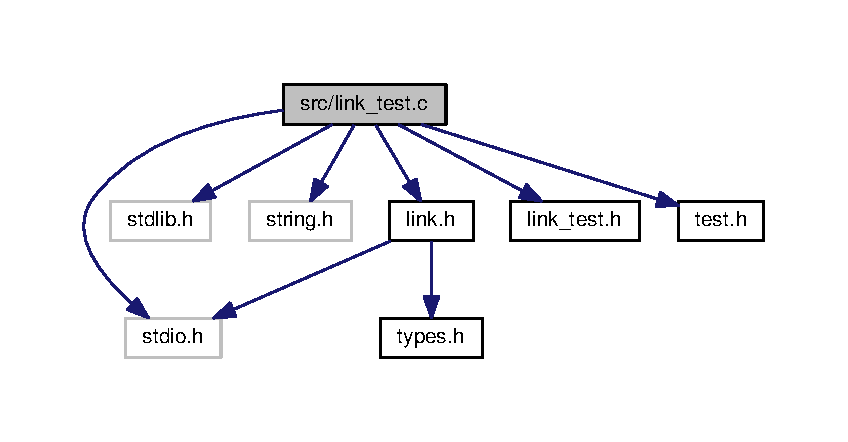
\includegraphics[width=350pt]{link__test_8c__incl}
\end{center}
\end{figure}
\subsection*{Macros}
\begin{DoxyCompactItemize}
\item 
\#define \hyperlink{link__test_8c_a2a77d2f2c5b698c69c19e1f8782bf709}{M\+A\+X\+\_\+\+T\+E\+S\+TS}~28
\end{DoxyCompactItemize}
\subsection*{Functions}
\begin{DoxyCompactItemize}
\item 
int \hyperlink{link__test_8c_a3c04138a5bfe5d72780bb7e82a18e627}{main} (int argc, char $\ast$$\ast$argv)
\begin{DoxyCompactList}\small\item\em Main function for L\+I\+NK unit tests. \end{DoxyCompactList}\item 
void \hyperlink{link__test_8c_a82c5ee441ad22caad8272212a9e9cc26}{test1\+\_\+link\+\_\+create} ()
\item 
void \hyperlink{link__test_8c_a24b5463da176c3e578b0a0fa8bb1f9f0}{test2\+\_\+link\+\_\+create} ()
\item 
void \hyperlink{link__test_8c_ae0e478a0540bed26befc071591e3ff6c}{test1\+\_\+link\+\_\+set\+\_\+name} ()
\item 
void \hyperlink{link__test_8c_aa66c1e991620a5a758ba6e4d6b4a8b73}{test2\+\_\+link\+\_\+set\+\_\+name} ()
\item 
void \hyperlink{link__test_8c_a8396e33f601deb52c940cb89cd7c6bfe}{test3\+\_\+link\+\_\+set\+\_\+name} ()
\item 
void \hyperlink{link__test_8c_a994aea17881a284366d11ac85d8c60a9}{test1\+\_\+link\+\_\+set\+\_\+link1} ()
\item 
void \hyperlink{link__test_8c_af0f992e367c55a169d9d3f1f4cf58d37}{test2\+\_\+link\+\_\+set\+\_\+link1} ()
\item 
void \hyperlink{link__test_8c_a4e44e515a644abf600efd18aaca7963a}{test1\+\_\+link\+\_\+set\+\_\+link2} ()
\item 
void \hyperlink{link__test_8c_ac4fcf188fc807162c5c279962367faa0}{test2\+\_\+link\+\_\+set\+\_\+link2} ()
\item 
void \hyperlink{link__test_8c_a3b39fdba0c3c967716572bfb01beec27}{test1\+\_\+link\+\_\+set\+\_\+status} ()
\item 
void \hyperlink{link__test_8c_a315ea19cd24434d2153b5df9f372a561}{test2\+\_\+link\+\_\+set\+\_\+status} ()
\item 
void \hyperlink{link__test_8c_a044128db00a5cc385d7157dea8bdf3c3}{test1\+\_\+link\+\_\+get\+\_\+name} ()
\item 
void \hyperlink{link__test_8c_a4efc6cfcdc210e2803f9d285734c571e}{test2\+\_\+link\+\_\+get\+\_\+name} ()
\item 
void \hyperlink{link__test_8c_a4e076db559af261fc8e6994cf9cde12c}{test1\+\_\+link\+\_\+get\+\_\+link1} ()
\item 
void \hyperlink{link__test_8c_a7e180eb974324d38e9bec8bada8d2f7a}{test2\+\_\+link\+\_\+get\+\_\+link1} ()
\item 
void \hyperlink{link__test_8c_a7a8a4b1f4730d248d2c7d648ee4da602}{test1\+\_\+link\+\_\+get\+\_\+link2} ()
\item 
void \hyperlink{link__test_8c_ab74179d7a6e4ceff70117cd20b82c95b}{test2\+\_\+link\+\_\+get\+\_\+link2} ()
\item 
void \hyperlink{link__test_8c_a19c70f79fd51d123173f7aaf6ae50bf8}{test1\+\_\+link\+\_\+get\+\_\+id} ()
\item 
void \hyperlink{link__test_8c_a0f967a1782dd7264e73ad428d22d125d}{test2\+\_\+link\+\_\+get\+\_\+id} ()
\item 
void \hyperlink{link__test_8c_ad4ca02e93472a080362a005ea4840218}{test1\+\_\+link\+\_\+destroy} ()
\item 
void \hyperlink{link__test_8c_afae7294e1213cade145448511cfae536}{test2\+\_\+link\+\_\+destroy} ()
\item 
void \hyperlink{link__test_8c_af99aa73f22b107610780db4877e34448}{test1\+\_\+link\+\_\+print} ()
\item 
void \hyperlink{link__test_8c_a0e42040390aae2aae9f0adee136fe359}{test1\+\_\+link\+\_\+set\+\_\+key} ()
\item 
void \hyperlink{link__test_8c_a502c73e4043204f9fa22f744506bf4e9}{test2\+\_\+link\+\_\+set\+\_\+key} ()
\item 
void \hyperlink{link__test_8c_ab9c08837de834dc139566cefae8e25c2}{test3\+\_\+link\+\_\+set\+\_\+key} ()
\item 
void \hyperlink{link__test_8c_a7dbdc2cfa491e66bba605d96304cf9a9}{test1\+\_\+link\+\_\+get\+\_\+key} ()
\item 
void \hyperlink{link__test_8c_abae02eb503ca35d9198dd4cb2f1c8d5e}{test2\+\_\+link\+\_\+get\+\_\+key} ()
\item 
void \hyperlink{link__test_8c_ac096b0cd1e6b6b44682dc43191a94296}{test3\+\_\+link\+\_\+get\+\_\+key} ()
\end{DoxyCompactItemize}


\subsection{Detailed Description}
It tests link module. 

\begin{DoxyAuthor}{Author}
Andres Mena 
\end{DoxyAuthor}
\begin{DoxyVersion}{Version}
1.\+0 
\end{DoxyVersion}
\begin{DoxyDate}{Date}
29-\/03-\/2018 
\end{DoxyDate}
\begin{DoxyCopyright}{Copyright}
G\+NU Public License 
\end{DoxyCopyright}


\subsection{Macro Definition Documentation}
\index{link\+\_\+test.\+c@{link\+\_\+test.\+c}!M\+A\+X\+\_\+\+T\+E\+S\+TS@{M\+A\+X\+\_\+\+T\+E\+S\+TS}}
\index{M\+A\+X\+\_\+\+T\+E\+S\+TS@{M\+A\+X\+\_\+\+T\+E\+S\+TS}!link\+\_\+test.\+c@{link\+\_\+test.\+c}}
\subsubsection[{\texorpdfstring{M\+A\+X\+\_\+\+T\+E\+S\+TS}{MAX_TESTS}}]{\setlength{\rightskip}{0pt plus 5cm}\#define M\+A\+X\+\_\+\+T\+E\+S\+TS~28}\hypertarget{link__test_8c_a2a77d2f2c5b698c69c19e1f8782bf709}{}\label{link__test_8c_a2a77d2f2c5b698c69c19e1f8782bf709}
Max amount of tests posible 

\subsection{Function Documentation}
\index{link\+\_\+test.\+c@{link\+\_\+test.\+c}!main@{main}}
\index{main@{main}!link\+\_\+test.\+c@{link\+\_\+test.\+c}}
\subsubsection[{\texorpdfstring{main(int argc, char $\ast$$\ast$argv)}{main(int argc, char **argv)}}]{\setlength{\rightskip}{0pt plus 5cm}int main (
\begin{DoxyParamCaption}
\item[{int}]{argc, }
\item[{char $\ast$$\ast$}]{argv}
\end{DoxyParamCaption}
)}\hypertarget{link__test_8c_a3c04138a5bfe5d72780bb7e82a18e627}{}\label{link__test_8c_a3c04138a5bfe5d72780bb7e82a18e627}


Main function for L\+I\+NK unit tests. 

You may execute A\+LL or a S\+I\+N\+G\+LE test 1.-\/ No parameter -\/$>$ A\+LL test are executed 2.-\/ A number means a particular test (the one identified by that number) is executed \index{link\+\_\+test.\+c@{link\+\_\+test.\+c}!test1\+\_\+link\+\_\+create@{test1\+\_\+link\+\_\+create}}
\index{test1\+\_\+link\+\_\+create@{test1\+\_\+link\+\_\+create}!link\+\_\+test.\+c@{link\+\_\+test.\+c}}
\subsubsection[{\texorpdfstring{test1\+\_\+link\+\_\+create()}{test1_link_create()}}]{\setlength{\rightskip}{0pt plus 5cm}void test1\+\_\+link\+\_\+create (
\begin{DoxyParamCaption}
{}
\end{DoxyParamCaption}
)}\hypertarget{link__test_8c_a82c5ee441ad22caad8272212a9e9cc26}{}\label{link__test_8c_a82c5ee441ad22caad8272212a9e9cc26}
\begin{DoxyRefDesc}{Test}
\item[\hyperlink{test__test000022}{Test}]Test link creation \end{DoxyRefDesc}
\begin{DoxyPrecond}{Precondition}
N\+O\+\_\+\+ID 
\end{DoxyPrecond}
\begin{DoxyPostcond}{Postcondition}
N\+U\+LL pointer to link 
\end{DoxyPostcond}
\index{link\+\_\+test.\+c@{link\+\_\+test.\+c}!test1\+\_\+link\+\_\+destroy@{test1\+\_\+link\+\_\+destroy}}
\index{test1\+\_\+link\+\_\+destroy@{test1\+\_\+link\+\_\+destroy}!link\+\_\+test.\+c@{link\+\_\+test.\+c}}
\subsubsection[{\texorpdfstring{test1\+\_\+link\+\_\+destroy()}{test1_link_destroy()}}]{\setlength{\rightskip}{0pt plus 5cm}void test1\+\_\+link\+\_\+destroy (
\begin{DoxyParamCaption}
{}
\end{DoxyParamCaption}
)}\hypertarget{link__test_8c_ad4ca02e93472a080362a005ea4840218}{}\label{link__test_8c_ad4ca02e93472a080362a005ea4840218}
\begin{DoxyRefDesc}{Test}
\item[\hyperlink{test__test000041}{Test}]Test function for destroying link \end{DoxyRefDesc}
\begin{DoxyPrecond}{Precondition}
N\+U\+LL pointer to link 
\end{DoxyPrecond}
\begin{DoxyPostcond}{Postcondition}
E\+R\+R\+OR 
\end{DoxyPostcond}
\index{link\+\_\+test.\+c@{link\+\_\+test.\+c}!test1\+\_\+link\+\_\+get\+\_\+id@{test1\+\_\+link\+\_\+get\+\_\+id}}
\index{test1\+\_\+link\+\_\+get\+\_\+id@{test1\+\_\+link\+\_\+get\+\_\+id}!link\+\_\+test.\+c@{link\+\_\+test.\+c}}
\subsubsection[{\texorpdfstring{test1\+\_\+link\+\_\+get\+\_\+id()}{test1_link_get_id()}}]{\setlength{\rightskip}{0pt plus 5cm}void test1\+\_\+link\+\_\+get\+\_\+id (
\begin{DoxyParamCaption}
{}
\end{DoxyParamCaption}
)}\hypertarget{link__test_8c_a19c70f79fd51d123173f7aaf6ae50bf8}{}\label{link__test_8c_a19c70f79fd51d123173f7aaf6ae50bf8}
\begin{DoxyRefDesc}{Test}
\item[\hyperlink{test__test000039}{Test}]Test function for getting link id \end{DoxyRefDesc}
\begin{DoxyPrecond}{Precondition}
Pointer to link 
\end{DoxyPrecond}
\begin{DoxyPostcond}{Postcondition}
link\+\_\+\+ID == Supplied link Id 
\end{DoxyPostcond}
\index{link\+\_\+test.\+c@{link\+\_\+test.\+c}!test1\+\_\+link\+\_\+get\+\_\+key@{test1\+\_\+link\+\_\+get\+\_\+key}}
\index{test1\+\_\+link\+\_\+get\+\_\+key@{test1\+\_\+link\+\_\+get\+\_\+key}!link\+\_\+test.\+c@{link\+\_\+test.\+c}}
\subsubsection[{\texorpdfstring{test1\+\_\+link\+\_\+get\+\_\+key()}{test1_link_get_key()}}]{\setlength{\rightskip}{0pt plus 5cm}void test1\+\_\+link\+\_\+get\+\_\+key (
\begin{DoxyParamCaption}
{}
\end{DoxyParamCaption}
)}\hypertarget{link__test_8c_a7dbdc2cfa491e66bba605d96304cf9a9}{}\label{link__test_8c_a7dbdc2cfa491e66bba605d96304cf9a9}
\begin{DoxyRefDesc}{Test}
\item[\hyperlink{test__test000047}{Test}]Test function for getting link key \end{DoxyRefDesc}
\begin{DoxyPrecond}{Precondition}
null Pointer to link 
\end{DoxyPrecond}
\begin{DoxyPostcond}{Postcondition}
N\+O\+\_\+\+ID 
\end{DoxyPostcond}
\index{link\+\_\+test.\+c@{link\+\_\+test.\+c}!test1\+\_\+link\+\_\+get\+\_\+link1@{test1\+\_\+link\+\_\+get\+\_\+link1}}
\index{test1\+\_\+link\+\_\+get\+\_\+link1@{test1\+\_\+link\+\_\+get\+\_\+link1}!link\+\_\+test.\+c@{link\+\_\+test.\+c}}
\subsubsection[{\texorpdfstring{test1\+\_\+link\+\_\+get\+\_\+link1()}{test1_link_get_link1()}}]{\setlength{\rightskip}{0pt plus 5cm}void test1\+\_\+link\+\_\+get\+\_\+link1 (
\begin{DoxyParamCaption}
{}
\end{DoxyParamCaption}
)}\hypertarget{link__test_8c_a4e076db559af261fc8e6994cf9cde12c}{}\label{link__test_8c_a4e076db559af261fc8e6994cf9cde12c}
\begin{DoxyRefDesc}{Test}
\item[\hyperlink{test__test000035}{Test}]Test function for getting first link \end{DoxyRefDesc}
\begin{DoxyPrecond}{Precondition}
Link pointer (with first link created) 
\end{DoxyPrecond}
\begin{DoxyPostcond}{Postcondition}
id of first link 
\end{DoxyPostcond}
\index{link\+\_\+test.\+c@{link\+\_\+test.\+c}!test1\+\_\+link\+\_\+get\+\_\+link2@{test1\+\_\+link\+\_\+get\+\_\+link2}}
\index{test1\+\_\+link\+\_\+get\+\_\+link2@{test1\+\_\+link\+\_\+get\+\_\+link2}!link\+\_\+test.\+c@{link\+\_\+test.\+c}}
\subsubsection[{\texorpdfstring{test1\+\_\+link\+\_\+get\+\_\+link2()}{test1_link_get_link2()}}]{\setlength{\rightskip}{0pt plus 5cm}void test1\+\_\+link\+\_\+get\+\_\+link2 (
\begin{DoxyParamCaption}
{}
\end{DoxyParamCaption}
)}\hypertarget{link__test_8c_a7a8a4b1f4730d248d2c7d648ee4da602}{}\label{link__test_8c_a7a8a4b1f4730d248d2c7d648ee4da602}
\begin{DoxyRefDesc}{Test}
\item[\hyperlink{test__test000037}{Test}]Test function for getting second link \end{DoxyRefDesc}
\begin{DoxyPrecond}{Precondition}
Link pointer (with second link created) 
\end{DoxyPrecond}
\begin{DoxyPostcond}{Postcondition}
id of second link 
\end{DoxyPostcond}
\index{link\+\_\+test.\+c@{link\+\_\+test.\+c}!test1\+\_\+link\+\_\+get\+\_\+name@{test1\+\_\+link\+\_\+get\+\_\+name}}
\index{test1\+\_\+link\+\_\+get\+\_\+name@{test1\+\_\+link\+\_\+get\+\_\+name}!link\+\_\+test.\+c@{link\+\_\+test.\+c}}
\subsubsection[{\texorpdfstring{test1\+\_\+link\+\_\+get\+\_\+name()}{test1_link_get_name()}}]{\setlength{\rightskip}{0pt plus 5cm}void test1\+\_\+link\+\_\+get\+\_\+name (
\begin{DoxyParamCaption}
{}
\end{DoxyParamCaption}
)}\hypertarget{link__test_8c_a044128db00a5cc385d7157dea8bdf3c3}{}\label{link__test_8c_a044128db00a5cc385d7157dea8bdf3c3}
\begin{DoxyRefDesc}{Test}
\item[\hyperlink{test__test000033}{Test}]Test function for link\+\_\+name obtaining \end{DoxyRefDesc}
\begin{DoxyPrecond}{Precondition}
Link pointer 
\end{DoxyPrecond}
\begin{DoxyPostcond}{Postcondition}
String with name 
\end{DoxyPostcond}
\index{link\+\_\+test.\+c@{link\+\_\+test.\+c}!test1\+\_\+link\+\_\+print@{test1\+\_\+link\+\_\+print}}
\index{test1\+\_\+link\+\_\+print@{test1\+\_\+link\+\_\+print}!link\+\_\+test.\+c@{link\+\_\+test.\+c}}
\subsubsection[{\texorpdfstring{test1\+\_\+link\+\_\+print()}{test1_link_print()}}]{\setlength{\rightskip}{0pt plus 5cm}void test1\+\_\+link\+\_\+print (
\begin{DoxyParamCaption}
{}
\end{DoxyParamCaption}
)}\hypertarget{link__test_8c_af99aa73f22b107610780db4877e34448}{}\label{link__test_8c_af99aa73f22b107610780db4877e34448}
\begin{DoxyRefDesc}{Test}
\item[\hyperlink{test__test000043}{Test}]Test function for printing link \end{DoxyRefDesc}
\begin{DoxyPrecond}{Precondition}
N\+U\+LL pointer to link 
\end{DoxyPrecond}
\begin{DoxyPostcond}{Postcondition}
E\+R\+R\+OR 
\end{DoxyPostcond}
\index{link\+\_\+test.\+c@{link\+\_\+test.\+c}!test1\+\_\+link\+\_\+set\+\_\+key@{test1\+\_\+link\+\_\+set\+\_\+key}}
\index{test1\+\_\+link\+\_\+set\+\_\+key@{test1\+\_\+link\+\_\+set\+\_\+key}!link\+\_\+test.\+c@{link\+\_\+test.\+c}}
\subsubsection[{\texorpdfstring{test1\+\_\+link\+\_\+set\+\_\+key()}{test1_link_set_key()}}]{\setlength{\rightskip}{0pt plus 5cm}void test1\+\_\+link\+\_\+set\+\_\+key (
\begin{DoxyParamCaption}
{}
\end{DoxyParamCaption}
)}\hypertarget{link__test_8c_a0e42040390aae2aae9f0adee136fe359}{}\label{link__test_8c_a0e42040390aae2aae9f0adee136fe359}
\begin{DoxyRefDesc}{Test}
\item[\hyperlink{test__test000044}{Test}]Test function for setting link key \end{DoxyRefDesc}
\begin{DoxyPrecond}{Precondition}
N\+U\+LL pointer to link 
\end{DoxyPrecond}
\begin{DoxyPostcond}{Postcondition}
E\+R\+R\+OR 
\end{DoxyPostcond}
\index{link\+\_\+test.\+c@{link\+\_\+test.\+c}!test1\+\_\+link\+\_\+set\+\_\+link1@{test1\+\_\+link\+\_\+set\+\_\+link1}}
\index{test1\+\_\+link\+\_\+set\+\_\+link1@{test1\+\_\+link\+\_\+set\+\_\+link1}!link\+\_\+test.\+c@{link\+\_\+test.\+c}}
\subsubsection[{\texorpdfstring{test1\+\_\+link\+\_\+set\+\_\+link1()}{test1_link_set_link1()}}]{\setlength{\rightskip}{0pt plus 5cm}void test1\+\_\+link\+\_\+set\+\_\+link1 (
\begin{DoxyParamCaption}
{}
\end{DoxyParamCaption}
)}\hypertarget{link__test_8c_a994aea17881a284366d11ac85d8c60a9}{}\label{link__test_8c_a994aea17881a284366d11ac85d8c60a9}
\begin{DoxyRefDesc}{Test}
\item[\hyperlink{test__test000027}{Test}]Test function for setting first link \end{DoxyRefDesc}
\begin{DoxyPrecond}{Precondition}
pointer to link and id 
\end{DoxyPrecond}
\begin{DoxyPostcond}{Postcondition}
Ouput==OK 
\end{DoxyPostcond}
\index{link\+\_\+test.\+c@{link\+\_\+test.\+c}!test1\+\_\+link\+\_\+set\+\_\+link2@{test1\+\_\+link\+\_\+set\+\_\+link2}}
\index{test1\+\_\+link\+\_\+set\+\_\+link2@{test1\+\_\+link\+\_\+set\+\_\+link2}!link\+\_\+test.\+c@{link\+\_\+test.\+c}}
\subsubsection[{\texorpdfstring{test1\+\_\+link\+\_\+set\+\_\+link2()}{test1_link_set_link2()}}]{\setlength{\rightskip}{0pt plus 5cm}void test1\+\_\+link\+\_\+set\+\_\+link2 (
\begin{DoxyParamCaption}
{}
\end{DoxyParamCaption}
)}\hypertarget{link__test_8c_a4e44e515a644abf600efd18aaca7963a}{}\label{link__test_8c_a4e44e515a644abf600efd18aaca7963a}
\begin{DoxyRefDesc}{Test}
\item[\hyperlink{test__test000029}{Test}]Test function for setting second link \end{DoxyRefDesc}
\begin{DoxyPrecond}{Precondition}
pointer to link and id 
\end{DoxyPrecond}
\begin{DoxyPostcond}{Postcondition}
Ouput==OK 
\end{DoxyPostcond}
\index{link\+\_\+test.\+c@{link\+\_\+test.\+c}!test1\+\_\+link\+\_\+set\+\_\+name@{test1\+\_\+link\+\_\+set\+\_\+name}}
\index{test1\+\_\+link\+\_\+set\+\_\+name@{test1\+\_\+link\+\_\+set\+\_\+name}!link\+\_\+test.\+c@{link\+\_\+test.\+c}}
\subsubsection[{\texorpdfstring{test1\+\_\+link\+\_\+set\+\_\+name()}{test1_link_set_name()}}]{\setlength{\rightskip}{0pt plus 5cm}void test1\+\_\+link\+\_\+set\+\_\+name (
\begin{DoxyParamCaption}
{}
\end{DoxyParamCaption}
)}\hypertarget{link__test_8c_ae0e478a0540bed26befc071591e3ff6c}{}\label{link__test_8c_ae0e478a0540bed26befc071591e3ff6c}
\begin{DoxyRefDesc}{Test}
\item[\hyperlink{test__test000024}{Test}]Test function for link\+\_\+name setting \end{DoxyRefDesc}
\begin{DoxyPrecond}{Precondition}
pointer to link and string with link name 
\end{DoxyPrecond}
\begin{DoxyPostcond}{Postcondition}
Ouput==OK 
\end{DoxyPostcond}
\index{link\+\_\+test.\+c@{link\+\_\+test.\+c}!test1\+\_\+link\+\_\+set\+\_\+status@{test1\+\_\+link\+\_\+set\+\_\+status}}
\index{test1\+\_\+link\+\_\+set\+\_\+status@{test1\+\_\+link\+\_\+set\+\_\+status}!link\+\_\+test.\+c@{link\+\_\+test.\+c}}
\subsubsection[{\texorpdfstring{test1\+\_\+link\+\_\+set\+\_\+status()}{test1_link_set_status()}}]{\setlength{\rightskip}{0pt plus 5cm}void test1\+\_\+link\+\_\+set\+\_\+status (
\begin{DoxyParamCaption}
{}
\end{DoxyParamCaption}
)}\hypertarget{link__test_8c_a3b39fdba0c3c967716572bfb01beec27}{}\label{link__test_8c_a3b39fdba0c3c967716572bfb01beec27}
\begin{DoxyRefDesc}{Test}
\item[\hyperlink{test__test000031}{Test}]Test function for setting status of link \end{DoxyRefDesc}
\begin{DoxyPrecond}{Precondition}
Pointer to link and L\+I\+N\+K\+\_\+\+ST 
\end{DoxyPrecond}
\begin{DoxyPostcond}{Postcondition}
Ouput==OK 
\end{DoxyPostcond}
\index{link\+\_\+test.\+c@{link\+\_\+test.\+c}!test2\+\_\+link\+\_\+create@{test2\+\_\+link\+\_\+create}}
\index{test2\+\_\+link\+\_\+create@{test2\+\_\+link\+\_\+create}!link\+\_\+test.\+c@{link\+\_\+test.\+c}}
\subsubsection[{\texorpdfstring{test2\+\_\+link\+\_\+create()}{test2_link_create()}}]{\setlength{\rightskip}{0pt plus 5cm}void test2\+\_\+link\+\_\+create (
\begin{DoxyParamCaption}
{}
\end{DoxyParamCaption}
)}\hypertarget{link__test_8c_a24b5463da176c3e578b0a0fa8bb1f9f0}{}\label{link__test_8c_a24b5463da176c3e578b0a0fa8bb1f9f0}
\begin{DoxyRefDesc}{Test}
\item[\hyperlink{test__test000023}{Test}]Test link creation \end{DoxyRefDesc}
\begin{DoxyPrecond}{Precondition}
ID 
\end{DoxyPrecond}
\begin{DoxyPostcond}{Postcondition}
link ID == id introduced 
\end{DoxyPostcond}
\index{link\+\_\+test.\+c@{link\+\_\+test.\+c}!test2\+\_\+link\+\_\+destroy@{test2\+\_\+link\+\_\+destroy}}
\index{test2\+\_\+link\+\_\+destroy@{test2\+\_\+link\+\_\+destroy}!link\+\_\+test.\+c@{link\+\_\+test.\+c}}
\subsubsection[{\texorpdfstring{test2\+\_\+link\+\_\+destroy()}{test2_link_destroy()}}]{\setlength{\rightskip}{0pt plus 5cm}void test2\+\_\+link\+\_\+destroy (
\begin{DoxyParamCaption}
{}
\end{DoxyParamCaption}
)}\hypertarget{link__test_8c_afae7294e1213cade145448511cfae536}{}\label{link__test_8c_afae7294e1213cade145448511cfae536}
\begin{DoxyRefDesc}{Test}
\item[\hyperlink{test__test000042}{Test}]Test function for destroying link \end{DoxyRefDesc}
\begin{DoxyPrecond}{Precondition}
pointer to link 
\end{DoxyPrecond}
\begin{DoxyPostcond}{Postcondition}
OK 
\end{DoxyPostcond}
\index{link\+\_\+test.\+c@{link\+\_\+test.\+c}!test2\+\_\+link\+\_\+get\+\_\+id@{test2\+\_\+link\+\_\+get\+\_\+id}}
\index{test2\+\_\+link\+\_\+get\+\_\+id@{test2\+\_\+link\+\_\+get\+\_\+id}!link\+\_\+test.\+c@{link\+\_\+test.\+c}}
\subsubsection[{\texorpdfstring{test2\+\_\+link\+\_\+get\+\_\+id()}{test2_link_get_id()}}]{\setlength{\rightskip}{0pt plus 5cm}void test2\+\_\+link\+\_\+get\+\_\+id (
\begin{DoxyParamCaption}
{}
\end{DoxyParamCaption}
)}\hypertarget{link__test_8c_a0f967a1782dd7264e73ad428d22d125d}{}\label{link__test_8c_a0f967a1782dd7264e73ad428d22d125d}
\begin{DoxyRefDesc}{Test}
\item[\hyperlink{test__test000040}{Test}]Test function for getting link id \end{DoxyRefDesc}
\begin{DoxyPrecond}{Precondition}
N\+U\+LL pointer to link 
\end{DoxyPrecond}
\begin{DoxyPostcond}{Postcondition}
N\+O\+\_\+\+ID 
\end{DoxyPostcond}
\index{link\+\_\+test.\+c@{link\+\_\+test.\+c}!test2\+\_\+link\+\_\+get\+\_\+key@{test2\+\_\+link\+\_\+get\+\_\+key}}
\index{test2\+\_\+link\+\_\+get\+\_\+key@{test2\+\_\+link\+\_\+get\+\_\+key}!link\+\_\+test.\+c@{link\+\_\+test.\+c}}
\subsubsection[{\texorpdfstring{test2\+\_\+link\+\_\+get\+\_\+key()}{test2_link_get_key()}}]{\setlength{\rightskip}{0pt plus 5cm}void test2\+\_\+link\+\_\+get\+\_\+key (
\begin{DoxyParamCaption}
{}
\end{DoxyParamCaption}
)}\hypertarget{link__test_8c_abae02eb503ca35d9198dd4cb2f1c8d5e}{}\label{link__test_8c_abae02eb503ca35d9198dd4cb2f1c8d5e}
\begin{DoxyRefDesc}{Test}
\item[\hyperlink{test__test000048}{Test}]Test function for getting link key \end{DoxyRefDesc}
\begin{DoxyPrecond}{Precondition}
Pointer to link 
\end{DoxyPrecond}
\begin{DoxyPostcond}{Postcondition}
Zero 
\end{DoxyPostcond}
\index{link\+\_\+test.\+c@{link\+\_\+test.\+c}!test2\+\_\+link\+\_\+get\+\_\+link1@{test2\+\_\+link\+\_\+get\+\_\+link1}}
\index{test2\+\_\+link\+\_\+get\+\_\+link1@{test2\+\_\+link\+\_\+get\+\_\+link1}!link\+\_\+test.\+c@{link\+\_\+test.\+c}}
\subsubsection[{\texorpdfstring{test2\+\_\+link\+\_\+get\+\_\+link1()}{test2_link_get_link1()}}]{\setlength{\rightskip}{0pt plus 5cm}void test2\+\_\+link\+\_\+get\+\_\+link1 (
\begin{DoxyParamCaption}
{}
\end{DoxyParamCaption}
)}\hypertarget{link__test_8c_a7e180eb974324d38e9bec8bada8d2f7a}{}\label{link__test_8c_a7e180eb974324d38e9bec8bada8d2f7a}
\begin{DoxyRefDesc}{Test}
\item[\hyperlink{test__test000036}{Test}]Test function for getting first link \end{DoxyRefDesc}
\begin{DoxyPrecond}{Precondition}
N\+U\+LL link pointer 
\end{DoxyPrecond}
\begin{DoxyPostcond}{Postcondition}
N\+O\+\_\+\+ID 
\end{DoxyPostcond}
\index{link\+\_\+test.\+c@{link\+\_\+test.\+c}!test2\+\_\+link\+\_\+get\+\_\+link2@{test2\+\_\+link\+\_\+get\+\_\+link2}}
\index{test2\+\_\+link\+\_\+get\+\_\+link2@{test2\+\_\+link\+\_\+get\+\_\+link2}!link\+\_\+test.\+c@{link\+\_\+test.\+c}}
\subsubsection[{\texorpdfstring{test2\+\_\+link\+\_\+get\+\_\+link2()}{test2_link_get_link2()}}]{\setlength{\rightskip}{0pt plus 5cm}void test2\+\_\+link\+\_\+get\+\_\+link2 (
\begin{DoxyParamCaption}
{}
\end{DoxyParamCaption}
)}\hypertarget{link__test_8c_ab74179d7a6e4ceff70117cd20b82c95b}{}\label{link__test_8c_ab74179d7a6e4ceff70117cd20b82c95b}
\begin{DoxyRefDesc}{Test}
\item[\hyperlink{test__test000038}{Test}]Test function for getting second link \end{DoxyRefDesc}
\begin{DoxyPrecond}{Precondition}
N\+U\+LL link pointer 
\end{DoxyPrecond}
\begin{DoxyPostcond}{Postcondition}
N\+O\+\_\+\+ID 
\end{DoxyPostcond}
\index{link\+\_\+test.\+c@{link\+\_\+test.\+c}!test2\+\_\+link\+\_\+get\+\_\+name@{test2\+\_\+link\+\_\+get\+\_\+name}}
\index{test2\+\_\+link\+\_\+get\+\_\+name@{test2\+\_\+link\+\_\+get\+\_\+name}!link\+\_\+test.\+c@{link\+\_\+test.\+c}}
\subsubsection[{\texorpdfstring{test2\+\_\+link\+\_\+get\+\_\+name()}{test2_link_get_name()}}]{\setlength{\rightskip}{0pt plus 5cm}void test2\+\_\+link\+\_\+get\+\_\+name (
\begin{DoxyParamCaption}
{}
\end{DoxyParamCaption}
)}\hypertarget{link__test_8c_a4efc6cfcdc210e2803f9d285734c571e}{}\label{link__test_8c_a4efc6cfcdc210e2803f9d285734c571e}
\begin{DoxyRefDesc}{Test}
\item[\hyperlink{test__test000034}{Test}]Test function for link\+\_\+name obtaining \end{DoxyRefDesc}
\begin{DoxyPrecond}{Precondition}
N\+U\+LL link pointer 
\end{DoxyPrecond}
\begin{DoxyPostcond}{Postcondition}
N\+U\+LL string 
\end{DoxyPostcond}
\index{link\+\_\+test.\+c@{link\+\_\+test.\+c}!test2\+\_\+link\+\_\+set\+\_\+key@{test2\+\_\+link\+\_\+set\+\_\+key}}
\index{test2\+\_\+link\+\_\+set\+\_\+key@{test2\+\_\+link\+\_\+set\+\_\+key}!link\+\_\+test.\+c@{link\+\_\+test.\+c}}
\subsubsection[{\texorpdfstring{test2\+\_\+link\+\_\+set\+\_\+key()}{test2_link_set_key()}}]{\setlength{\rightskip}{0pt plus 5cm}void test2\+\_\+link\+\_\+set\+\_\+key (
\begin{DoxyParamCaption}
{}
\end{DoxyParamCaption}
)}\hypertarget{link__test_8c_a502c73e4043204f9fa22f744506bf4e9}{}\label{link__test_8c_a502c73e4043204f9fa22f744506bf4e9}
\begin{DoxyRefDesc}{Test}
\item[\hyperlink{test__test000045}{Test}]Test function for setting link key \end{DoxyRefDesc}
\begin{DoxyPrecond}{Precondition}
Pointer to link and N\+O\+\_\+\+ID 
\end{DoxyPrecond}
\begin{DoxyPostcond}{Postcondition}
E\+R\+R\+OR 
\end{DoxyPostcond}
\index{link\+\_\+test.\+c@{link\+\_\+test.\+c}!test2\+\_\+link\+\_\+set\+\_\+link1@{test2\+\_\+link\+\_\+set\+\_\+link1}}
\index{test2\+\_\+link\+\_\+set\+\_\+link1@{test2\+\_\+link\+\_\+set\+\_\+link1}!link\+\_\+test.\+c@{link\+\_\+test.\+c}}
\subsubsection[{\texorpdfstring{test2\+\_\+link\+\_\+set\+\_\+link1()}{test2_link_set_link1()}}]{\setlength{\rightskip}{0pt plus 5cm}void test2\+\_\+link\+\_\+set\+\_\+link1 (
\begin{DoxyParamCaption}
{}
\end{DoxyParamCaption}
)}\hypertarget{link__test_8c_af0f992e367c55a169d9d3f1f4cf58d37}{}\label{link__test_8c_af0f992e367c55a169d9d3f1f4cf58d37}
\begin{DoxyRefDesc}{Test}
\item[\hyperlink{test__test000028}{Test}]Test function for setting first link \end{DoxyRefDesc}
\begin{DoxyPrecond}{Precondition}
N\+U\+LL pointer to link and id 
\end{DoxyPrecond}
\begin{DoxyPostcond}{Postcondition}
Ouput==E\+R\+R\+OR 
\end{DoxyPostcond}
\index{link\+\_\+test.\+c@{link\+\_\+test.\+c}!test2\+\_\+link\+\_\+set\+\_\+link2@{test2\+\_\+link\+\_\+set\+\_\+link2}}
\index{test2\+\_\+link\+\_\+set\+\_\+link2@{test2\+\_\+link\+\_\+set\+\_\+link2}!link\+\_\+test.\+c@{link\+\_\+test.\+c}}
\subsubsection[{\texorpdfstring{test2\+\_\+link\+\_\+set\+\_\+link2()}{test2_link_set_link2()}}]{\setlength{\rightskip}{0pt plus 5cm}void test2\+\_\+link\+\_\+set\+\_\+link2 (
\begin{DoxyParamCaption}
{}
\end{DoxyParamCaption}
)}\hypertarget{link__test_8c_ac4fcf188fc807162c5c279962367faa0}{}\label{link__test_8c_ac4fcf188fc807162c5c279962367faa0}
\begin{DoxyRefDesc}{Test}
\item[\hyperlink{test__test000030}{Test}]Test function for setting second link \end{DoxyRefDesc}
\begin{DoxyPrecond}{Precondition}
N\+U\+LL pointer to link and id 
\end{DoxyPrecond}
\begin{DoxyPostcond}{Postcondition}
Ouput==E\+R\+R\+OR 
\end{DoxyPostcond}
\index{link\+\_\+test.\+c@{link\+\_\+test.\+c}!test2\+\_\+link\+\_\+set\+\_\+name@{test2\+\_\+link\+\_\+set\+\_\+name}}
\index{test2\+\_\+link\+\_\+set\+\_\+name@{test2\+\_\+link\+\_\+set\+\_\+name}!link\+\_\+test.\+c@{link\+\_\+test.\+c}}
\subsubsection[{\texorpdfstring{test2\+\_\+link\+\_\+set\+\_\+name()}{test2_link_set_name()}}]{\setlength{\rightskip}{0pt plus 5cm}void test2\+\_\+link\+\_\+set\+\_\+name (
\begin{DoxyParamCaption}
{}
\end{DoxyParamCaption}
)}\hypertarget{link__test_8c_aa66c1e991620a5a758ba6e4d6b4a8b73}{}\label{link__test_8c_aa66c1e991620a5a758ba6e4d6b4a8b73}
\begin{DoxyRefDesc}{Test}
\item[\hyperlink{test__test000025}{Test}]Test function for link\+\_\+name setting \end{DoxyRefDesc}
\begin{DoxyPrecond}{Precondition}
N\+U\+LL pointer to link and string with link name 
\end{DoxyPrecond}
\begin{DoxyPostcond}{Postcondition}
Ouput==E\+R\+R\+OR 
\end{DoxyPostcond}
\index{link\+\_\+test.\+c@{link\+\_\+test.\+c}!test2\+\_\+link\+\_\+set\+\_\+status@{test2\+\_\+link\+\_\+set\+\_\+status}}
\index{test2\+\_\+link\+\_\+set\+\_\+status@{test2\+\_\+link\+\_\+set\+\_\+status}!link\+\_\+test.\+c@{link\+\_\+test.\+c}}
\subsubsection[{\texorpdfstring{test2\+\_\+link\+\_\+set\+\_\+status()}{test2_link_set_status()}}]{\setlength{\rightskip}{0pt plus 5cm}void test2\+\_\+link\+\_\+set\+\_\+status (
\begin{DoxyParamCaption}
{}
\end{DoxyParamCaption}
)}\hypertarget{link__test_8c_a315ea19cd24434d2153b5df9f372a561}{}\label{link__test_8c_a315ea19cd24434d2153b5df9f372a561}
\begin{DoxyRefDesc}{Test}
\item[\hyperlink{test__test000032}{Test}]Test function for setting status of link \end{DoxyRefDesc}
\begin{DoxyPrecond}{Precondition}
N\+U\+LL pointer to link and L\+I\+N\+K\+\_\+\+ST 
\end{DoxyPrecond}
\begin{DoxyPostcond}{Postcondition}
Ouput==E\+R\+R\+OR 
\end{DoxyPostcond}
\index{link\+\_\+test.\+c@{link\+\_\+test.\+c}!test3\+\_\+link\+\_\+get\+\_\+key@{test3\+\_\+link\+\_\+get\+\_\+key}}
\index{test3\+\_\+link\+\_\+get\+\_\+key@{test3\+\_\+link\+\_\+get\+\_\+key}!link\+\_\+test.\+c@{link\+\_\+test.\+c}}
\subsubsection[{\texorpdfstring{test3\+\_\+link\+\_\+get\+\_\+key()}{test3_link_get_key()}}]{\setlength{\rightskip}{0pt plus 5cm}void test3\+\_\+link\+\_\+get\+\_\+key (
\begin{DoxyParamCaption}
{}
\end{DoxyParamCaption}
)}\hypertarget{link__test_8c_ac096b0cd1e6b6b44682dc43191a94296}{}\label{link__test_8c_ac096b0cd1e6b6b44682dc43191a94296}
\begin{DoxyRefDesc}{Test}
\item[\hyperlink{test__test000049}{Test}]Test function for getting link key \end{DoxyRefDesc}
\begin{DoxyPrecond}{Precondition}
Pointer to link and introduced id 
\end{DoxyPrecond}
\begin{DoxyPostcond}{Postcondition}
Id previosuly introduced 
\end{DoxyPostcond}
\index{link\+\_\+test.\+c@{link\+\_\+test.\+c}!test3\+\_\+link\+\_\+set\+\_\+key@{test3\+\_\+link\+\_\+set\+\_\+key}}
\index{test3\+\_\+link\+\_\+set\+\_\+key@{test3\+\_\+link\+\_\+set\+\_\+key}!link\+\_\+test.\+c@{link\+\_\+test.\+c}}
\subsubsection[{\texorpdfstring{test3\+\_\+link\+\_\+set\+\_\+key()}{test3_link_set_key()}}]{\setlength{\rightskip}{0pt plus 5cm}void test3\+\_\+link\+\_\+set\+\_\+key (
\begin{DoxyParamCaption}
{}
\end{DoxyParamCaption}
)}\hypertarget{link__test_8c_ab9c08837de834dc139566cefae8e25c2}{}\label{link__test_8c_ab9c08837de834dc139566cefae8e25c2}
\begin{DoxyRefDesc}{Test}
\item[\hyperlink{test__test000046}{Test}]Test function for setting link key \end{DoxyRefDesc}
\begin{DoxyPrecond}{Precondition}
Pointer to link and ID 
\end{DoxyPrecond}
\begin{DoxyPostcond}{Postcondition}
OK 
\end{DoxyPostcond}
\index{link\+\_\+test.\+c@{link\+\_\+test.\+c}!test3\+\_\+link\+\_\+set\+\_\+name@{test3\+\_\+link\+\_\+set\+\_\+name}}
\index{test3\+\_\+link\+\_\+set\+\_\+name@{test3\+\_\+link\+\_\+set\+\_\+name}!link\+\_\+test.\+c@{link\+\_\+test.\+c}}
\subsubsection[{\texorpdfstring{test3\+\_\+link\+\_\+set\+\_\+name()}{test3_link_set_name()}}]{\setlength{\rightskip}{0pt plus 5cm}void test3\+\_\+link\+\_\+set\+\_\+name (
\begin{DoxyParamCaption}
{}
\end{DoxyParamCaption}
)}\hypertarget{link__test_8c_a8396e33f601deb52c940cb89cd7c6bfe}{}\label{link__test_8c_a8396e33f601deb52c940cb89cd7c6bfe}
\begin{DoxyRefDesc}{Test}
\item[\hyperlink{test__test000026}{Test}]Test function for link\+\_\+name setting \end{DoxyRefDesc}
\begin{DoxyPrecond}{Precondition}
pointer to link and N\+U\+LL string of characters 
\end{DoxyPrecond}
\begin{DoxyPostcond}{Postcondition}
Ouput==E\+R\+R\+OR 
\end{DoxyPostcond}

\hypertarget{object_8c}{}\section{src/object.c File Reference}
\label{object_8c}\index{src/object.\+c@{src/object.\+c}}


Implements the game object commands.  


{\ttfamily \#include $<$stdio.\+h$>$}\\*
{\ttfamily \#include $<$stdlib.\+h$>$}\\*
{\ttfamily \#include $<$string.\+h$>$}\\*
{\ttfamily \#include \char`\"{}types.\+h\char`\"{}}\\*
{\ttfamily \#include \char`\"{}object.\+h\char`\"{}}\\*
{\ttfamily \#include \char`\"{}game.\+h\char`\"{}}\\*
Include dependency graph for object.\+c\+:
\nopagebreak
\begin{figure}[H]
\begin{center}
\leavevmode
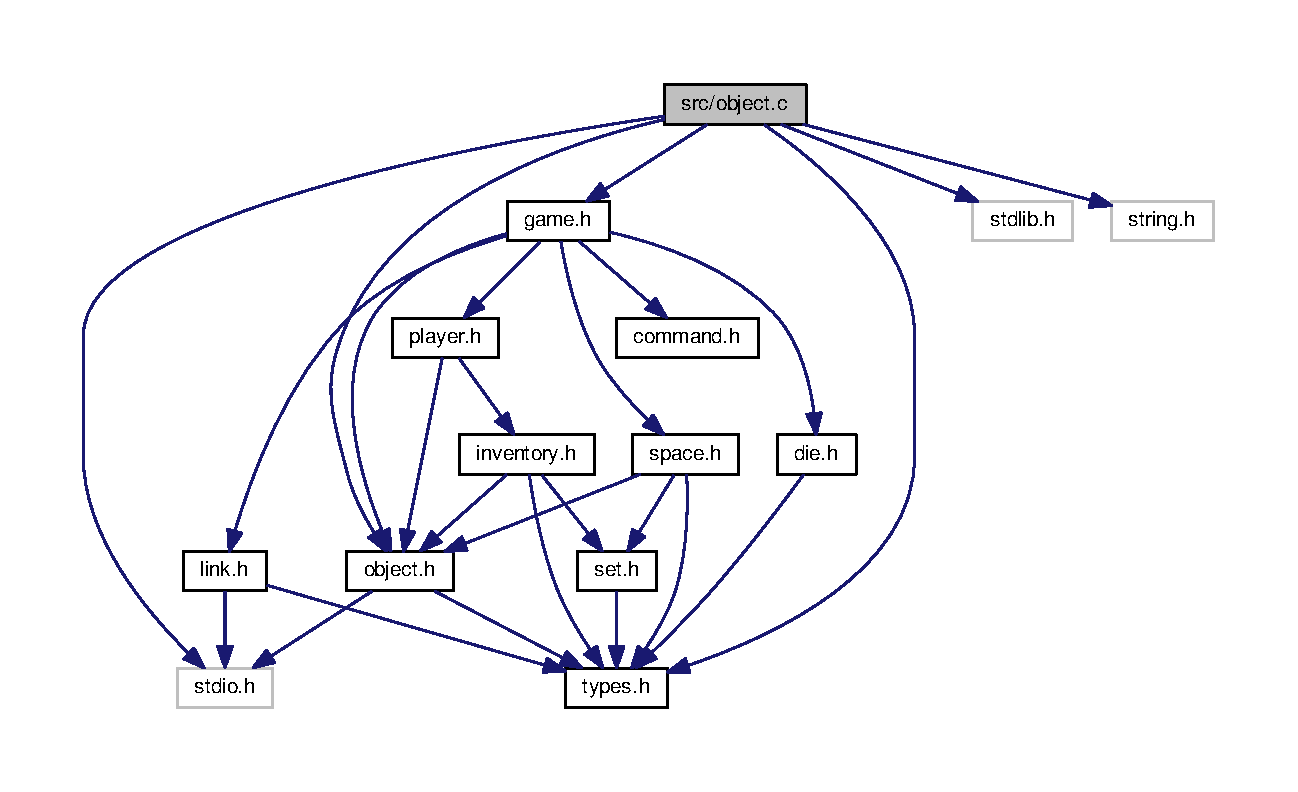
\includegraphics[width=350pt]{object_8c__incl}
\end{center}
\end{figure}
\subsection*{Data Structures}
\begin{DoxyCompactItemize}
\item 
struct \hyperlink{structObjectproperties}{Objectproperties}
\begin{DoxyCompactList}\small\item\em properties of the objects in the game \end{DoxyCompactList}\item 
struct \hyperlink{struct__Object}{\+\_\+\+Object}
\begin{DoxyCompactList}\small\item\em object of the game \end{DoxyCompactList}\end{DoxyCompactItemize}
\subsection*{Functions}
\begin{DoxyCompactItemize}
\item 
\hyperlink{object_8h_a7f8bbcda919b65ce67f92fba08e0212f}{Object} $\ast$ \hyperlink{object_8c_abb0cd30fca5fbddf137c6c04df66bbc7}{object\+\_\+create} (\hyperlink{types_8h_a845e604fb28f7e3d97549da3448149d3}{Id} id)
\begin{DoxyCompactList}\small\item\em creates an object \end{DoxyCompactList}\item 
void \hyperlink{object_8c_a26c44b44a0fbeb25ef0984614c752dfc}{object\+\_\+destroy} (\hyperlink{object_8h_a7f8bbcda919b65ce67f92fba08e0212f}{Object} $\ast$o)
\begin{DoxyCompactList}\small\item\em frees memory \end{DoxyCompactList}\item 
\hyperlink{types_8h_a845e604fb28f7e3d97549da3448149d3}{Id} \hyperlink{object_8c_a9752f952077d92e3caad01bc0ef88219}{object\+\_\+get\+\_\+id} (\hyperlink{object_8h_a7f8bbcda919b65ce67f92fba08e0212f}{Object} $\ast$o)
\begin{DoxyCompactList}\small\item\em gets the id of an object \end{DoxyCompactList}\item 
\hyperlink{types_8h_a845e604fb28f7e3d97549da3448149d3}{Id} \hyperlink{object_8c_a0f486e12d9d5db67ed56f40b5cdc0f7f}{object\+\_\+get\+\_\+original\+\_\+position} (\hyperlink{object_8h_a7f8bbcda919b65ce67f92fba08e0212f}{Object} $\ast$o)
\begin{DoxyCompactList}\small\item\em gets description \end{DoxyCompactList}\item 
\hyperlink{types_8h_a845e604fb28f7e3d97549da3448149d3}{Id} \hyperlink{object_8c_acf961fc31f1928c71c59d96a2ff0d1cd}{object\+\_\+get\+\_\+location} (\hyperlink{object_8h_a7f8bbcda919b65ce67f92fba08e0212f}{Object} $\ast$o)
\begin{DoxyCompactList}\small\item\em gets the location of an object \end{DoxyCompactList}\item 
char $\ast$ \hyperlink{object_8c_a1d9c831b8ea3bc3667c4bf166bd458dd}{object\+\_\+get\+\_\+name} (\hyperlink{object_8h_a7f8bbcda919b65ce67f92fba08e0212f}{Object} $\ast$o)
\begin{DoxyCompactList}\small\item\em gets the name of an object \end{DoxyCompactList}\item 
char $\ast$ \hyperlink{object_8c_a66311e7f25b9eba333bc2ddec8aba14f}{object\+\_\+get\+\_\+original\+\_\+description} (\hyperlink{object_8h_a7f8bbcda919b65ce67f92fba08e0212f}{Object} $\ast$o)
\begin{DoxyCompactList}\small\item\em gets description \end{DoxyCompactList}\item 
char $\ast$ \hyperlink{object_8c_ac1254bf414022a80a5e3d07887c89121}{object\+\_\+get\+\_\+moved\+\_\+description} (\hyperlink{object_8h_a7f8bbcda919b65ce67f92fba08e0212f}{Object} $\ast$o)
\begin{DoxyCompactList}\small\item\em gets description \end{DoxyCompactList}\item 
\hyperlink{types_8h_a32c27cc471df37f4fc818d65de0a56c4}{S\+T\+A\+T\+US} \hyperlink{object_8c_a8d07c8e2c06363c4a41b36198e57fc10}{object\+\_\+set\+\_\+id} (\hyperlink{object_8h_a7f8bbcda919b65ce67f92fba08e0212f}{Object} $\ast$o, \hyperlink{types_8h_a845e604fb28f7e3d97549da3448149d3}{Id} id)
\begin{DoxyCompactList}\small\item\em sets an id for an object \end{DoxyCompactList}\item 
\hyperlink{types_8h_a32c27cc471df37f4fc818d65de0a56c4}{S\+T\+A\+T\+US} \hyperlink{object_8c_a0a4d910353d6334df5831468ff5524f9}{object\+\_\+set\+\_\+location} (\hyperlink{object_8h_a7f8bbcda919b65ce67f92fba08e0212f}{Object} $\ast$o, \hyperlink{types_8h_a845e604fb28f7e3d97549da3448149d3}{Id} id)
\begin{DoxyCompactList}\small\item\em sets location \end{DoxyCompactList}\item 
\hyperlink{types_8h_a32c27cc471df37f4fc818d65de0a56c4}{S\+T\+A\+T\+US} \hyperlink{object_8c_a169ccd54cbbdc828f67fd819ede6000d}{object\+\_\+set\+\_\+original\+\_\+position} (\hyperlink{object_8h_a7f8bbcda919b65ce67f92fba08e0212f}{Object} $\ast$o, \hyperlink{types_8h_a845e604fb28f7e3d97549da3448149d3}{Id} id)
\begin{DoxyCompactList}\small\item\em sets position \end{DoxyCompactList}\item 
\hyperlink{types_8h_a32c27cc471df37f4fc818d65de0a56c4}{S\+T\+A\+T\+US} \hyperlink{object_8c_a839f09c377c10dc0138e844c5c2f9324}{object\+\_\+set\+\_\+name} (\hyperlink{object_8h_a7f8bbcda919b65ce67f92fba08e0212f}{Object} $\ast$o, char $\ast$name)
\begin{DoxyCompactList}\small\item\em sets the name of an object \end{DoxyCompactList}\item 
\hyperlink{types_8h_a32c27cc471df37f4fc818d65de0a56c4}{S\+T\+A\+T\+US} \hyperlink{object_8c_ae70e3276ecd61873f1f0a540ee785e3f}{object\+\_\+set\+\_\+original\+\_\+description} (\hyperlink{object_8h_a7f8bbcda919b65ce67f92fba08e0212f}{Object} $\ast$o, char $\ast$description)
\begin{DoxyCompactList}\small\item\em sets description \end{DoxyCompactList}\item 
\hyperlink{types_8h_a32c27cc471df37f4fc818d65de0a56c4}{S\+T\+A\+T\+US} \hyperlink{object_8c_a684297abcecea4f985c22c09d7a2683e}{object\+\_\+set\+\_\+moved\+\_\+description} (\hyperlink{object_8h_a7f8bbcda919b65ce67f92fba08e0212f}{Object} $\ast$o, char $\ast$description)
\begin{DoxyCompactList}\small\item\em sets description \end{DoxyCompactList}\item 
\hyperlink{types_8h_a32c27cc471df37f4fc818d65de0a56c4}{S\+T\+A\+T\+US} \hyperlink{object_8c_a259c9fd13df4766071af2e0a0d7a1a87}{object\+\_\+set\+\_\+prop\+\_\+\+Movable} (\hyperlink{object_8h_a7f8bbcda919b65ce67f92fba08e0212f}{Object} $\ast$o, \hyperlink{types_8h_a3e5b8192e7d9ffaf3542f1210aec18dd}{B\+O\+OL} st)
\begin{DoxyCompactList}\small\item\em sets status of mobility \end{DoxyCompactList}\item 
\hyperlink{types_8h_a3e5b8192e7d9ffaf3542f1210aec18dd}{B\+O\+OL} \hyperlink{object_8c_a98f562a9ee1801aea8f5f0212bdba008}{object\+\_\+get\+\_\+prop\+\_\+\+Movable} (\hyperlink{object_8h_a7f8bbcda919b65ce67f92fba08e0212f}{Object} $\ast$o)
\begin{DoxyCompactList}\small\item\em gets the mobility status \end{DoxyCompactList}\item 
\hyperlink{types_8h_a32c27cc471df37f4fc818d65de0a56c4}{S\+T\+A\+T\+US} \hyperlink{object_8c_a2b49f5b9d0eba678c034bdf9c91b36b1}{object\+\_\+set\+\_\+prop\+\_\+\+Moved} (\hyperlink{object_8h_a7f8bbcda919b65ce67f92fba08e0212f}{Object} $\ast$o, \hyperlink{types_8h_a3e5b8192e7d9ffaf3542f1210aec18dd}{B\+O\+OL} st)
\begin{DoxyCompactList}\small\item\em sets status of being moved \end{DoxyCompactList}\item 
\hyperlink{types_8h_a3e5b8192e7d9ffaf3542f1210aec18dd}{B\+O\+OL} \hyperlink{object_8c_a6dcd51ad45ff363d05ad96ca06ee56f5}{object\+\_\+get\+\_\+prop\+\_\+\+Moved} (\hyperlink{object_8h_a7f8bbcda919b65ce67f92fba08e0212f}{Object} $\ast$o)
\begin{DoxyCompactList}\small\item\em gets the moved object \end{DoxyCompactList}\item 
\hyperlink{types_8h_a32c27cc471df37f4fc818d65de0a56c4}{S\+T\+A\+T\+US} \hyperlink{object_8c_a1514debf4d64d167eaf1dce61e0675df}{object\+\_\+set\+\_\+prop\+\_\+\+Hidden} (\hyperlink{object_8h_a7f8bbcda919b65ce67f92fba08e0212f}{Object} $\ast$o, \hyperlink{types_8h_a3e5b8192e7d9ffaf3542f1210aec18dd}{B\+O\+OL} st)
\begin{DoxyCompactList}\small\item\em sets status of hidden \end{DoxyCompactList}\item 
\hyperlink{types_8h_a3e5b8192e7d9ffaf3542f1210aec18dd}{B\+O\+OL} \hyperlink{object_8c_a9a6ddffc3ac22a73f1161e1efda8b92d}{object\+\_\+get\+\_\+prop\+\_\+\+Hidden} (\hyperlink{object_8h_a7f8bbcda919b65ce67f92fba08e0212f}{Object} $\ast$o)
\begin{DoxyCompactList}\small\item\em gets the hidden status \end{DoxyCompactList}\item 
\hyperlink{types_8h_a32c27cc471df37f4fc818d65de0a56c4}{S\+T\+A\+T\+US} \hyperlink{object_8c_a7a1071b9008fced8261ba7ea1b3f20b0}{object\+\_\+set\+\_\+prop\+\_\+\+Illuminate} (\hyperlink{object_8h_a7f8bbcda919b65ce67f92fba08e0212f}{Object} $\ast$o, \hyperlink{types_8h_a3e5b8192e7d9ffaf3542f1210aec18dd}{B\+O\+OL} st)
\begin{DoxyCompactList}\small\item\em sets status of ilumination \end{DoxyCompactList}\item 
\hyperlink{types_8h_a3e5b8192e7d9ffaf3542f1210aec18dd}{B\+O\+OL} \hyperlink{object_8c_af6837f83ac2983f6e3214a16257afa59}{object\+\_\+get\+\_\+prop\+\_\+\+Illuminate} (\hyperlink{object_8h_a7f8bbcda919b65ce67f92fba08e0212f}{Object} $\ast$o)
\begin{DoxyCompactList}\small\item\em gets the ilumination status \end{DoxyCompactList}\item 
\hyperlink{types_8h_a32c27cc471df37f4fc818d65de0a56c4}{S\+T\+A\+T\+US} \hyperlink{object_8c_ae8d09d72e32a824c6eac741a623747ed}{object\+\_\+set\+\_\+prop\+\_\+\+Switched\+On} (\hyperlink{object_8h_a7f8bbcda919b65ce67f92fba08e0212f}{Object} $\ast$o, \hyperlink{types_8h_a3e5b8192e7d9ffaf3542f1210aec18dd}{B\+O\+OL} st)
\begin{DoxyCompactList}\small\item\em sets status of switching on \end{DoxyCompactList}\item 
\hyperlink{types_8h_a3e5b8192e7d9ffaf3542f1210aec18dd}{B\+O\+OL} \hyperlink{object_8c_a85049c1ca7de81feec4e99e9951491c0}{object\+\_\+get\+\_\+prop\+\_\+\+Switched\+On} (\hyperlink{object_8h_a7f8bbcda919b65ce67f92fba08e0212f}{Object} $\ast$o)
\begin{DoxyCompactList}\small\item\em gets the switched on status \end{DoxyCompactList}\item 
\hyperlink{types_8h_a32c27cc471df37f4fc818d65de0a56c4}{S\+T\+A\+T\+US} \hyperlink{object_8c_a7ada936990bfb9c93bf2f188de1a585b}{object\+\_\+set\+\_\+prop\+\_\+\+Open} (\hyperlink{object_8h_a7f8bbcda919b65ce67f92fba08e0212f}{Object} $\ast$o, \hyperlink{types_8h_a845e604fb28f7e3d97549da3448149d3}{Id} id)
\begin{DoxyCompactList}\small\item\em sets status of opening \end{DoxyCompactList}\item 
\hyperlink{types_8h_a845e604fb28f7e3d97549da3448149d3}{Id} \hyperlink{object_8c_a1ab2ce1f8aa99b8502044a6a78ff4993}{object\+\_\+get\+\_\+prop\+\_\+\+Open} (\hyperlink{object_8h_a7f8bbcda919b65ce67f92fba08e0212f}{Object} $\ast$o)
\begin{DoxyCompactList}\small\item\em gets the opened object \end{DoxyCompactList}\item 
\hyperlink{types_8h_a32c27cc471df37f4fc818d65de0a56c4}{S\+T\+A\+T\+US} \hyperlink{object_8c_a4a4f1a7f753ec9295548c099ec755718}{object\+\_\+print} (\hyperlink{object_8h_a7f8bbcda919b65ce67f92fba08e0212f}{Object} $\ast$o, F\+I\+LE $\ast$f)
\begin{DoxyCompactList}\small\item\em prints an object \end{DoxyCompactList}\end{DoxyCompactItemize}


\subsection{Detailed Description}
Implements the game object commands. 

The object module has all the functions that helps us manage the objects with a better organisation.

\begin{DoxyAuthor}{Author}
Juan Moreno 
\end{DoxyAuthor}
\begin{DoxyVersion}{Version}
1.\+6 
\end{DoxyVersion}
\begin{DoxyDate}{Date}
07-\/04-\/2018 
\end{DoxyDate}


\subsection{Function Documentation}
\index{object.\+c@{object.\+c}!object\+\_\+create@{object\+\_\+create}}
\index{object\+\_\+create@{object\+\_\+create}!object.\+c@{object.\+c}}
\subsubsection[{\texorpdfstring{object\+\_\+create(\+Id id)}{object_create(Id id)}}]{\setlength{\rightskip}{0pt plus 5cm}{\bf Object}$\ast$ object\+\_\+create (
\begin{DoxyParamCaption}
\item[{{\bf Id}}]{id}
\end{DoxyParamCaption}
)}\hypertarget{object_8c_abb0cd30fca5fbddf137c6c04df66bbc7}{}\label{object_8c_abb0cd30fca5fbddf137c6c04df66bbc7}


creates an object 

It creates a new object initializing the variables of the structure, checks is something goes wrong and if it does go wrong, returns N\+U\+LL.

\begin{DoxyAuthor}{Author}
Juan Moreno 
\end{DoxyAuthor}

\begin{DoxyParams}{Parameters}
{\em id} & long int. \\
\hline
\end{DoxyParams}
\begin{DoxyReturn}{Returns}
Pointer to object, N\+U\+LL if something goes wrong. 
\end{DoxyReturn}
\index{object.\+c@{object.\+c}!object\+\_\+destroy@{object\+\_\+destroy}}
\index{object\+\_\+destroy@{object\+\_\+destroy}!object.\+c@{object.\+c}}
\subsubsection[{\texorpdfstring{object\+\_\+destroy(\+Object $\ast$o)}{object_destroy(Object *o)}}]{\setlength{\rightskip}{0pt plus 5cm}void object\+\_\+destroy (
\begin{DoxyParamCaption}
\item[{{\bf Object} $\ast$}]{o}
\end{DoxyParamCaption}
)}\hypertarget{object_8c_a26c44b44a0fbeb25ef0984614c752dfc}{}\label{object_8c_a26c44b44a0fbeb25ef0984614c752dfc}


frees memory 

Receives pointer to object and frees the memory it occupied.

\begin{DoxyAuthor}{Author}
Juan Moreno 
\end{DoxyAuthor}

\begin{DoxyParams}{Parameters}
{\em o} & pointer to object. \\
\hline
\end{DoxyParams}
\begin{DoxyReturn}{Returns}
void function. 
\end{DoxyReturn}
\index{object.\+c@{object.\+c}!object\+\_\+get\+\_\+id@{object\+\_\+get\+\_\+id}}
\index{object\+\_\+get\+\_\+id@{object\+\_\+get\+\_\+id}!object.\+c@{object.\+c}}
\subsubsection[{\texorpdfstring{object\+\_\+get\+\_\+id(\+Object $\ast$o)}{object_get_id(Object *o)}}]{\setlength{\rightskip}{0pt plus 5cm}{\bf Id} object\+\_\+get\+\_\+id (
\begin{DoxyParamCaption}
\item[{{\bf Object} $\ast$}]{o}
\end{DoxyParamCaption}
)}\hypertarget{object_8c_a9752f952077d92e3caad01bc0ef88219}{}\label{object_8c_a9752f952077d92e3caad01bc0ef88219}


gets the id of an object 

Function in charge of getting the id of an object by using a pointer to object.

\begin{DoxyAuthor}{Author}
Juan Moreno 
\end{DoxyAuthor}

\begin{DoxyParams}{Parameters}
{\em o} & pointer to object. \\
\hline
\end{DoxyParams}
\begin{DoxyReturn}{Returns}
Id, N\+O\+\_\+\+ID if object is pointing N\+U\+LL. 
\end{DoxyReturn}
\index{object.\+c@{object.\+c}!object\+\_\+get\+\_\+location@{object\+\_\+get\+\_\+location}}
\index{object\+\_\+get\+\_\+location@{object\+\_\+get\+\_\+location}!object.\+c@{object.\+c}}
\subsubsection[{\texorpdfstring{object\+\_\+get\+\_\+location(\+Object $\ast$o)}{object_get_location(Object *o)}}]{\setlength{\rightskip}{0pt plus 5cm}{\bf Id} object\+\_\+get\+\_\+location (
\begin{DoxyParamCaption}
\item[{{\bf Object} $\ast$}]{o}
\end{DoxyParamCaption}
)}\hypertarget{object_8c_acf961fc31f1928c71c59d96a2ff0d1cd}{}\label{object_8c_acf961fc31f1928c71c59d96a2ff0d1cd}


gets the location of an object 

Function in charge of getting the location of an object and returning it.

\begin{DoxyAuthor}{Author}
Juan Moreno 
\end{DoxyAuthor}

\begin{DoxyParams}{Parameters}
{\em o} & pointer to object. \\
\hline
\end{DoxyParams}
\begin{DoxyReturn}{Returns}
Id, N\+O\+\_\+\+ID if inventory is pointing N\+U\+LL. 
\end{DoxyReturn}
\index{object.\+c@{object.\+c}!object\+\_\+get\+\_\+moved\+\_\+description@{object\+\_\+get\+\_\+moved\+\_\+description}}
\index{object\+\_\+get\+\_\+moved\+\_\+description@{object\+\_\+get\+\_\+moved\+\_\+description}!object.\+c@{object.\+c}}
\subsubsection[{\texorpdfstring{object\+\_\+get\+\_\+moved\+\_\+description(\+Object $\ast$o)}{object_get_moved_description(Object *o)}}]{\setlength{\rightskip}{0pt plus 5cm}char$\ast$ object\+\_\+get\+\_\+moved\+\_\+description (
\begin{DoxyParamCaption}
\item[{{\bf Object} $\ast$}]{o}
\end{DoxyParamCaption}
)}\hypertarget{object_8c_ac1254bf414022a80a5e3d07887c89121}{}\label{object_8c_ac1254bf414022a80a5e3d07887c89121}


gets description 

Changes the description of the object that has already been created.

\begin{DoxyAuthor}{Author}
Juan Moreno 
\end{DoxyAuthor}

\begin{DoxyParams}{Parameters}
{\em o} & pointer to object. \\
\hline
\end{DoxyParams}
\begin{DoxyReturn}{Returns}
the description of the object (char). 
\end{DoxyReturn}
\index{object.\+c@{object.\+c}!object\+\_\+get\+\_\+name@{object\+\_\+get\+\_\+name}}
\index{object\+\_\+get\+\_\+name@{object\+\_\+get\+\_\+name}!object.\+c@{object.\+c}}
\subsubsection[{\texorpdfstring{object\+\_\+get\+\_\+name(\+Object $\ast$o)}{object_get_name(Object *o)}}]{\setlength{\rightskip}{0pt plus 5cm}char$\ast$ object\+\_\+get\+\_\+name (
\begin{DoxyParamCaption}
\item[{{\bf Object} $\ast$}]{o}
\end{DoxyParamCaption}
)}\hypertarget{object_8c_a1d9c831b8ea3bc3667c4bf166bd458dd}{}\label{object_8c_a1d9c831b8ea3bc3667c4bf166bd458dd}


gets the name of an object 

Function in charge of showing the name of an object that has already been set.

\begin{DoxyAuthor}{Author}
Juan Moreno 
\end{DoxyAuthor}

\begin{DoxyParams}{Parameters}
{\em o} & pointer to object. \\
\hline
\end{DoxyParams}
\begin{DoxyReturn}{Returns}
char (name of the object). 
\end{DoxyReturn}
\index{object.\+c@{object.\+c}!object\+\_\+get\+\_\+original\+\_\+description@{object\+\_\+get\+\_\+original\+\_\+description}}
\index{object\+\_\+get\+\_\+original\+\_\+description@{object\+\_\+get\+\_\+original\+\_\+description}!object.\+c@{object.\+c}}
\subsubsection[{\texorpdfstring{object\+\_\+get\+\_\+original\+\_\+description(\+Object $\ast$o)}{object_get_original_description(Object *o)}}]{\setlength{\rightskip}{0pt plus 5cm}char$\ast$ object\+\_\+get\+\_\+original\+\_\+description (
\begin{DoxyParamCaption}
\item[{{\bf Object} $\ast$}]{o}
\end{DoxyParamCaption}
)}\hypertarget{object_8c_a66311e7f25b9eba333bc2ddec8aba14f}{}\label{object_8c_a66311e7f25b9eba333bc2ddec8aba14f}


gets description 

Changes the description of the object that has already been created.

\begin{DoxyAuthor}{Author}
Juan Moreno 
\end{DoxyAuthor}

\begin{DoxyParams}{Parameters}
{\em o} & pointer to object. \\
\hline
\end{DoxyParams}
\begin{DoxyReturn}{Returns}
the description of the object (char). 
\end{DoxyReturn}
\index{object.\+c@{object.\+c}!object\+\_\+get\+\_\+original\+\_\+position@{object\+\_\+get\+\_\+original\+\_\+position}}
\index{object\+\_\+get\+\_\+original\+\_\+position@{object\+\_\+get\+\_\+original\+\_\+position}!object.\+c@{object.\+c}}
\subsubsection[{\texorpdfstring{object\+\_\+get\+\_\+original\+\_\+position(\+Object $\ast$o)}{object_get_original_position(Object *o)}}]{\setlength{\rightskip}{0pt plus 5cm}{\bf Id} object\+\_\+get\+\_\+original\+\_\+position (
\begin{DoxyParamCaption}
\item[{{\bf Object} $\ast$}]{o}
\end{DoxyParamCaption}
)}\hypertarget{object_8c_a0f486e12d9d5db67ed56f40b5cdc0f7f}{}\label{object_8c_a0f486e12d9d5db67ed56f40b5cdc0f7f}


gets description 

It returns the description that has already been set for an object.

\begin{DoxyAuthor}{Author}
Juan Moreno 
\end{DoxyAuthor}

\begin{DoxyParams}{Parameters}
{\em o} & pointer to object. \\
\hline
\end{DoxyParams}
\begin{DoxyReturn}{Returns}
pointer to char, string of characters that return the description of the object. 
\end{DoxyReturn}
\index{object.\+c@{object.\+c}!object\+\_\+get\+\_\+prop\+\_\+\+Hidden@{object\+\_\+get\+\_\+prop\+\_\+\+Hidden}}
\index{object\+\_\+get\+\_\+prop\+\_\+\+Hidden@{object\+\_\+get\+\_\+prop\+\_\+\+Hidden}!object.\+c@{object.\+c}}
\subsubsection[{\texorpdfstring{object\+\_\+get\+\_\+prop\+\_\+\+Hidden(\+Object $\ast$o)}{object_get_prop_Hidden(Object *o)}}]{\setlength{\rightskip}{0pt plus 5cm}{\bf B\+O\+OL} object\+\_\+get\+\_\+prop\+\_\+\+Hidden (
\begin{DoxyParamCaption}
\item[{{\bf Object} $\ast$}]{o}
\end{DoxyParamCaption}
)}\hypertarget{object_8c_a9a6ddffc3ac22a73f1161e1efda8b92d}{}\label{object_8c_a9a6ddffc3ac22a73f1161e1efda8b92d}


gets the hidden status 

Function that returns a hidden object.

\begin{DoxyAuthor}{Author}
Juan Moreno 
\end{DoxyAuthor}

\begin{DoxyParams}{Parameters}
{\em o} & pointer to object. \\
\hline
\end{DoxyParams}
\begin{DoxyReturn}{Returns}
B\+O\+OL, F\+A\+L\+SE if when checking is not correct, if it is correct, T\+R\+UE. 
\end{DoxyReturn}
\index{object.\+c@{object.\+c}!object\+\_\+get\+\_\+prop\+\_\+\+Illuminate@{object\+\_\+get\+\_\+prop\+\_\+\+Illuminate}}
\index{object\+\_\+get\+\_\+prop\+\_\+\+Illuminate@{object\+\_\+get\+\_\+prop\+\_\+\+Illuminate}!object.\+c@{object.\+c}}
\subsubsection[{\texorpdfstring{object\+\_\+get\+\_\+prop\+\_\+\+Illuminate(\+Object $\ast$o)}{object_get_prop_Illuminate(Object *o)}}]{\setlength{\rightskip}{0pt plus 5cm}{\bf B\+O\+OL} object\+\_\+get\+\_\+prop\+\_\+\+Illuminate (
\begin{DoxyParamCaption}
\item[{{\bf Object} $\ast$}]{o}
\end{DoxyParamCaption}
)}\hypertarget{object_8c_af6837f83ac2983f6e3214a16257afa59}{}\label{object_8c_af6837f83ac2983f6e3214a16257afa59}


gets the ilumination status 

Function that returns an iluminated object.

\begin{DoxyAuthor}{Author}
Juan Moreno 
\end{DoxyAuthor}

\begin{DoxyParams}{Parameters}
{\em o} & pointer to object. \\
\hline
\end{DoxyParams}
\begin{DoxyReturn}{Returns}
B\+O\+OL, F\+A\+L\+SE if when checking is not correct, if it is correct, T\+R\+UE. 
\end{DoxyReturn}
\index{object.\+c@{object.\+c}!object\+\_\+get\+\_\+prop\+\_\+\+Movable@{object\+\_\+get\+\_\+prop\+\_\+\+Movable}}
\index{object\+\_\+get\+\_\+prop\+\_\+\+Movable@{object\+\_\+get\+\_\+prop\+\_\+\+Movable}!object.\+c@{object.\+c}}
\subsubsection[{\texorpdfstring{object\+\_\+get\+\_\+prop\+\_\+\+Movable(\+Object $\ast$o)}{object_get_prop_Movable(Object *o)}}]{\setlength{\rightskip}{0pt plus 5cm}{\bf B\+O\+OL} object\+\_\+get\+\_\+prop\+\_\+\+Movable (
\begin{DoxyParamCaption}
\item[{{\bf Object} $\ast$}]{o}
\end{DoxyParamCaption}
)}\hypertarget{object_8c_a98f562a9ee1801aea8f5f0212bdba008}{}\label{object_8c_a98f562a9ee1801aea8f5f0212bdba008}


gets the mobility status 

Function that returns whether an object is movable or not.

\begin{DoxyAuthor}{Author}
Juan Moreno 
\end{DoxyAuthor}

\begin{DoxyParams}{Parameters}
{\em o} & pointer to object. \\
\hline
\end{DoxyParams}
\begin{DoxyReturn}{Returns}
B\+O\+OL, F\+A\+L\+SE if when checking is not correct, if it is correct, T\+R\+UE. 
\end{DoxyReturn}
\index{object.\+c@{object.\+c}!object\+\_\+get\+\_\+prop\+\_\+\+Moved@{object\+\_\+get\+\_\+prop\+\_\+\+Moved}}
\index{object\+\_\+get\+\_\+prop\+\_\+\+Moved@{object\+\_\+get\+\_\+prop\+\_\+\+Moved}!object.\+c@{object.\+c}}
\subsubsection[{\texorpdfstring{object\+\_\+get\+\_\+prop\+\_\+\+Moved(\+Object $\ast$o)}{object_get_prop_Moved(Object *o)}}]{\setlength{\rightskip}{0pt plus 5cm}{\bf B\+O\+OL} object\+\_\+get\+\_\+prop\+\_\+\+Moved (
\begin{DoxyParamCaption}
\item[{{\bf Object} $\ast$}]{o}
\end{DoxyParamCaption}
)}\hypertarget{object_8c_a6dcd51ad45ff363d05ad96ca06ee56f5}{}\label{object_8c_a6dcd51ad45ff363d05ad96ca06ee56f5}


gets the moved object 

Function that returns the moved object that you already know that can be movable.

\begin{DoxyAuthor}{Author}
Juan Moreno 
\end{DoxyAuthor}

\begin{DoxyParams}{Parameters}
{\em o} & pointer to object. \\
\hline
\end{DoxyParams}
\begin{DoxyReturn}{Returns}
B\+O\+OL, F\+A\+L\+SE if when checking is not correct, if it is correct, T\+R\+UE. 
\end{DoxyReturn}
\index{object.\+c@{object.\+c}!object\+\_\+get\+\_\+prop\+\_\+\+Open@{object\+\_\+get\+\_\+prop\+\_\+\+Open}}
\index{object\+\_\+get\+\_\+prop\+\_\+\+Open@{object\+\_\+get\+\_\+prop\+\_\+\+Open}!object.\+c@{object.\+c}}
\subsubsection[{\texorpdfstring{object\+\_\+get\+\_\+prop\+\_\+\+Open(\+Object $\ast$o)}{object_get_prop_Open(Object *o)}}]{\setlength{\rightskip}{0pt plus 5cm}{\bf Id} object\+\_\+get\+\_\+prop\+\_\+\+Open (
\begin{DoxyParamCaption}
\item[{{\bf Object} $\ast$}]{o}
\end{DoxyParamCaption}
)}\hypertarget{object_8c_a1ab2ce1f8aa99b8502044a6a78ff4993}{}\label{object_8c_a1ab2ce1f8aa99b8502044a6a78ff4993}


gets the opened object 

It gets the position of the objects which is defined in data.\+dat file that can be opened.

\begin{DoxyAuthor}{Author}
Juan Moreno 
\end{DoxyAuthor}

\begin{DoxyParams}{Parameters}
{\em o} & pointer to object. \\
\hline
\end{DoxyParams}
\begin{DoxyReturn}{Returns}
Id, N\+O\+\_\+\+ID if inventory is pointing N\+U\+LL. 
\end{DoxyReturn}
\index{object.\+c@{object.\+c}!object\+\_\+get\+\_\+prop\+\_\+\+Switched\+On@{object\+\_\+get\+\_\+prop\+\_\+\+Switched\+On}}
\index{object\+\_\+get\+\_\+prop\+\_\+\+Switched\+On@{object\+\_\+get\+\_\+prop\+\_\+\+Switched\+On}!object.\+c@{object.\+c}}
\subsubsection[{\texorpdfstring{object\+\_\+get\+\_\+prop\+\_\+\+Switched\+On(\+Object $\ast$o)}{object_get_prop_SwitchedOn(Object *o)}}]{\setlength{\rightskip}{0pt plus 5cm}{\bf B\+O\+OL} object\+\_\+get\+\_\+prop\+\_\+\+Switched\+On (
\begin{DoxyParamCaption}
\item[{{\bf Object} $\ast$}]{o}
\end{DoxyParamCaption}
)}\hypertarget{object_8c_a85049c1ca7de81feec4e99e9951491c0}{}\label{object_8c_a85049c1ca7de81feec4e99e9951491c0}


gets the switched on status 

Function that returns a status that can be iluminated and also is switched on.

\begin{DoxyAuthor}{Author}
Juan Moreno 
\end{DoxyAuthor}

\begin{DoxyParams}{Parameters}
{\em o} & pointer to object. \\
\hline
\end{DoxyParams}
\begin{DoxyReturn}{Returns}
B\+O\+OL, F\+A\+L\+SE if when checking is not correct, if it is correct, T\+R\+UE. 
\end{DoxyReturn}
\index{object.\+c@{object.\+c}!object\+\_\+print@{object\+\_\+print}}
\index{object\+\_\+print@{object\+\_\+print}!object.\+c@{object.\+c}}
\subsubsection[{\texorpdfstring{object\+\_\+print(\+Object $\ast$o, F\+I\+L\+E $\ast$f)}{object_print(Object *o, FILE *f)}}]{\setlength{\rightskip}{0pt plus 5cm}{\bf S\+T\+A\+T\+US} object\+\_\+print (
\begin{DoxyParamCaption}
\item[{{\bf Object} $\ast$}]{o, }
\item[{F\+I\+LE $\ast$}]{f}
\end{DoxyParamCaption}
)}\hypertarget{object_8c_a4a4f1a7f753ec9295548c099ec755718}{}\label{object_8c_a4a4f1a7f753ec9295548c099ec755718}


prints an object 

Writes the object data, used for debugging.

\begin{DoxyAuthor}{Author}
Juan Moreno 
\end{DoxyAuthor}

\begin{DoxyParams}{Parameters}
{\em o} & pointer to object. \\
\hline
{\em f} & file to write the object. \\
\hline
\end{DoxyParams}
\begin{DoxyReturn}{Returns}
S\+T\+A\+T\+US, E\+R\+R\+OR if argument received is N\+U\+LL, if not, OK. 
\end{DoxyReturn}
\index{object.\+c@{object.\+c}!object\+\_\+set\+\_\+id@{object\+\_\+set\+\_\+id}}
\index{object\+\_\+set\+\_\+id@{object\+\_\+set\+\_\+id}!object.\+c@{object.\+c}}
\subsubsection[{\texorpdfstring{object\+\_\+set\+\_\+id(\+Object $\ast$o, Id id)}{object_set_id(Object *o, Id id)}}]{\setlength{\rightskip}{0pt plus 5cm}{\bf S\+T\+A\+T\+US} object\+\_\+set\+\_\+id (
\begin{DoxyParamCaption}
\item[{{\bf Object} $\ast$}]{o, }
\item[{{\bf Id}}]{id}
\end{DoxyParamCaption}
)}\hypertarget{object_8c_a8d07c8e2c06363c4a41b36198e57fc10}{}\label{object_8c_a8d07c8e2c06363c4a41b36198e57fc10}


sets an id for an object 

It spececifically changes the id of a particular object.

\begin{DoxyAuthor}{Author}
Juan Moreno 
\end{DoxyAuthor}

\begin{DoxyParams}{Parameters}
{\em o} & pointer to object. \\
\hline
{\em id} & long int. \\
\hline
\end{DoxyParams}
\begin{DoxyReturn}{Returns}
S\+T\+A\+T\+US, E\+R\+R\+OR if argument received is N\+U\+LL, if not, OK. 
\end{DoxyReturn}
\index{object.\+c@{object.\+c}!object\+\_\+set\+\_\+location@{object\+\_\+set\+\_\+location}}
\index{object\+\_\+set\+\_\+location@{object\+\_\+set\+\_\+location}!object.\+c@{object.\+c}}
\subsubsection[{\texorpdfstring{object\+\_\+set\+\_\+location(\+Object $\ast$o, Id id)}{object_set_location(Object *o, Id id)}}]{\setlength{\rightskip}{0pt plus 5cm}{\bf S\+T\+A\+T\+US} object\+\_\+set\+\_\+location (
\begin{DoxyParamCaption}
\item[{{\bf Object} $\ast$}]{o, }
\item[{{\bf Id}}]{id}
\end{DoxyParamCaption}
)}\hypertarget{object_8c_a0a4d910353d6334df5831468ff5524f9}{}\label{object_8c_a0a4d910353d6334df5831468ff5524f9}


sets location 

Changes an object\textquotesingle{}s location ingame

\begin{DoxyAuthor}{Author}
Juan Moreno 
\end{DoxyAuthor}

\begin{DoxyParams}{Parameters}
{\em o} & pointer to object. \\
\hline
{\em id} & id of the object\textquotesingle{}s location. \\
\hline
\end{DoxyParams}
\begin{DoxyReturn}{Returns}
S\+T\+A\+T\+US, E\+R\+R\+OR if argument received is N\+U\+LL, if not, OK. 
\end{DoxyReturn}
\index{object.\+c@{object.\+c}!object\+\_\+set\+\_\+moved\+\_\+description@{object\+\_\+set\+\_\+moved\+\_\+description}}
\index{object\+\_\+set\+\_\+moved\+\_\+description@{object\+\_\+set\+\_\+moved\+\_\+description}!object.\+c@{object.\+c}}
\subsubsection[{\texorpdfstring{object\+\_\+set\+\_\+moved\+\_\+description(\+Object $\ast$o, char $\ast$description)}{object_set_moved_description(Object *o, char *description)}}]{\setlength{\rightskip}{0pt plus 5cm}{\bf S\+T\+A\+T\+US} object\+\_\+set\+\_\+moved\+\_\+description (
\begin{DoxyParamCaption}
\item[{{\bf Object} $\ast$}]{o, }
\item[{char $\ast$}]{description}
\end{DoxyParamCaption}
)}\hypertarget{object_8c_a684297abcecea4f985c22c09d7a2683e}{}\label{object_8c_a684297abcecea4f985c22c09d7a2683e}


sets description 

It prepares the description of an object that has been moved.

\begin{DoxyAuthor}{Author}
Juan Moreno 
\end{DoxyAuthor}

\begin{DoxyParams}{Parameters}
{\em o} & pointer to object. \\
\hline
{\em description} & pointer to char. \\
\hline
\end{DoxyParams}
\begin{DoxyReturn}{Returns}
S\+T\+A\+T\+US, E\+R\+R\+OR if argument received is N\+U\+LL, if not, OK. 
\end{DoxyReturn}
\index{object.\+c@{object.\+c}!object\+\_\+set\+\_\+name@{object\+\_\+set\+\_\+name}}
\index{object\+\_\+set\+\_\+name@{object\+\_\+set\+\_\+name}!object.\+c@{object.\+c}}
\subsubsection[{\texorpdfstring{object\+\_\+set\+\_\+name(\+Object $\ast$o, char $\ast$name)}{object_set_name(Object *o, char *name)}}]{\setlength{\rightskip}{0pt plus 5cm}{\bf S\+T\+A\+T\+US} object\+\_\+set\+\_\+name (
\begin{DoxyParamCaption}
\item[{{\bf Object} $\ast$}]{o, }
\item[{char $\ast$}]{name}
\end{DoxyParamCaption}
)}\hypertarget{object_8c_a839f09c377c10dc0138e844c5c2f9324}{}\label{object_8c_a839f09c377c10dc0138e844c5c2f9324}


sets the name of an object 

Modifies an object\textquotesingle{}s name in order to set an specific name por each object.

\begin{DoxyAuthor}{Author}
Juan Moreno 
\end{DoxyAuthor}

\begin{DoxyParams}{Parameters}
{\em o} & pointer to object. \\
\hline
{\em name} & name of the object(char). \\
\hline
\end{DoxyParams}
\begin{DoxyReturn}{Returns}
S\+T\+A\+T\+US, E\+R\+R\+OR if argument received is N\+U\+LL, if not, OK. 
\end{DoxyReturn}
\index{object.\+c@{object.\+c}!object\+\_\+set\+\_\+original\+\_\+description@{object\+\_\+set\+\_\+original\+\_\+description}}
\index{object\+\_\+set\+\_\+original\+\_\+description@{object\+\_\+set\+\_\+original\+\_\+description}!object.\+c@{object.\+c}}
\subsubsection[{\texorpdfstring{object\+\_\+set\+\_\+original\+\_\+description(\+Object $\ast$o, char $\ast$description)}{object_set_original_description(Object *o, char *description)}}]{\setlength{\rightskip}{0pt plus 5cm}{\bf S\+T\+A\+T\+US} object\+\_\+set\+\_\+original\+\_\+description (
\begin{DoxyParamCaption}
\item[{{\bf Object} $\ast$}]{o, }
\item[{char $\ast$}]{description}
\end{DoxyParamCaption}
)}\hypertarget{object_8c_ae70e3276ecd61873f1f0a540ee785e3f}{}\label{object_8c_ae70e3276ecd61873f1f0a540ee785e3f}


sets description 

It prepares the description of the objects which is defined in data.\+dat file. Principally describes what the objects do.

\begin{DoxyAuthor}{Author}
Juan Moreno 
\end{DoxyAuthor}

\begin{DoxyParams}{Parameters}
{\em o} & pointer to object. \\
\hline
{\em description} & char (description of the object). \\
\hline
\end{DoxyParams}
\begin{DoxyReturn}{Returns}
S\+T\+A\+T\+US, E\+R\+R\+OR if argument received is N\+U\+LL, if not, OK. 
\end{DoxyReturn}
\index{object.\+c@{object.\+c}!object\+\_\+set\+\_\+original\+\_\+position@{object\+\_\+set\+\_\+original\+\_\+position}}
\index{object\+\_\+set\+\_\+original\+\_\+position@{object\+\_\+set\+\_\+original\+\_\+position}!object.\+c@{object.\+c}}
\subsubsection[{\texorpdfstring{object\+\_\+set\+\_\+original\+\_\+position(\+Object $\ast$o, Id id)}{object_set_original_position(Object *o, Id id)}}]{\setlength{\rightskip}{0pt plus 5cm}{\bf S\+T\+A\+T\+US} object\+\_\+set\+\_\+original\+\_\+position (
\begin{DoxyParamCaption}
\item[{{\bf Object} $\ast$}]{o, }
\item[{{\bf Id}}]{id}
\end{DoxyParamCaption}
)}\hypertarget{object_8c_a169ccd54cbbdc828f67fd819ede6000d}{}\label{object_8c_a169ccd54cbbdc828f67fd819ede6000d}


sets position 

It prepares the position of the objects which is defined in data.\+dat file. Principally defines a position for the object.

\begin{DoxyAuthor}{Author}
Juan Moreno 
\end{DoxyAuthor}

\begin{DoxyParams}{Parameters}
{\em o} & pointer to object. \\
\hline
{\em id} & long int. \\
\hline
\end{DoxyParams}
\begin{DoxyReturn}{Returns}
S\+T\+A\+T\+US, E\+R\+R\+OR if argument received is N\+U\+LL, if not, OK. 
\end{DoxyReturn}
\index{object.\+c@{object.\+c}!object\+\_\+set\+\_\+prop\+\_\+\+Hidden@{object\+\_\+set\+\_\+prop\+\_\+\+Hidden}}
\index{object\+\_\+set\+\_\+prop\+\_\+\+Hidden@{object\+\_\+set\+\_\+prop\+\_\+\+Hidden}!object.\+c@{object.\+c}}
\subsubsection[{\texorpdfstring{object\+\_\+set\+\_\+prop\+\_\+\+Hidden(\+Object $\ast$o, B\+O\+O\+L st)}{object_set_prop_Hidden(Object *o, BOOL st)}}]{\setlength{\rightskip}{0pt plus 5cm}{\bf S\+T\+A\+T\+US} object\+\_\+set\+\_\+prop\+\_\+\+Hidden (
\begin{DoxyParamCaption}
\item[{{\bf Object} $\ast$}]{o, }
\item[{{\bf B\+O\+OL}}]{st}
\end{DoxyParamCaption}
)}\hypertarget{object_8c_a1514debf4d64d167eaf1dce61e0675df}{}\label{object_8c_a1514debf4d64d167eaf1dce61e0675df}


sets status of hidden 

It sets a new status to objects, a hidden status that allows the player to hide objects.

\begin{DoxyAuthor}{Author}
Juan Moreno 
\end{DoxyAuthor}

\begin{DoxyParams}{Parameters}
{\em o} & pointer to object. \\
\hline
{\em st} & Boolean \\
\hline
\end{DoxyParams}
\begin{DoxyReturn}{Returns}
S\+T\+A\+T\+US, E\+R\+R\+OR if argument received is N\+U\+LL, if not, OK. 
\end{DoxyReturn}
\index{object.\+c@{object.\+c}!object\+\_\+set\+\_\+prop\+\_\+\+Illuminate@{object\+\_\+set\+\_\+prop\+\_\+\+Illuminate}}
\index{object\+\_\+set\+\_\+prop\+\_\+\+Illuminate@{object\+\_\+set\+\_\+prop\+\_\+\+Illuminate}!object.\+c@{object.\+c}}
\subsubsection[{\texorpdfstring{object\+\_\+set\+\_\+prop\+\_\+\+Illuminate(\+Object $\ast$o, B\+O\+O\+L st)}{object_set_prop_Illuminate(Object *o, BOOL st)}}]{\setlength{\rightskip}{0pt plus 5cm}{\bf S\+T\+A\+T\+US} object\+\_\+set\+\_\+prop\+\_\+\+Illuminate (
\begin{DoxyParamCaption}
\item[{{\bf Object} $\ast$}]{o, }
\item[{{\bf B\+O\+OL}}]{st}
\end{DoxyParamCaption}
)}\hypertarget{object_8c_a7a1071b9008fced8261ba7ea1b3f20b0}{}\label{object_8c_a7a1071b9008fced8261ba7ea1b3f20b0}


sets status of ilumination 

It sets a new status to objects, an ilumination status that allows the player to iluminate objects.

\begin{DoxyAuthor}{Author}
Juan Moreno 
\end{DoxyAuthor}

\begin{DoxyParams}{Parameters}
{\em o} & pointer to object. \\
\hline
{\em st} & Boolean \\
\hline
\end{DoxyParams}
\begin{DoxyReturn}{Returns}
S\+T\+A\+T\+US, E\+R\+R\+OR if argument received is N\+U\+LL, if not, OK. 
\end{DoxyReturn}
\index{object.\+c@{object.\+c}!object\+\_\+set\+\_\+prop\+\_\+\+Movable@{object\+\_\+set\+\_\+prop\+\_\+\+Movable}}
\index{object\+\_\+set\+\_\+prop\+\_\+\+Movable@{object\+\_\+set\+\_\+prop\+\_\+\+Movable}!object.\+c@{object.\+c}}
\subsubsection[{\texorpdfstring{object\+\_\+set\+\_\+prop\+\_\+\+Movable(\+Object $\ast$o, B\+O\+O\+L st)}{object_set_prop_Movable(Object *o, BOOL st)}}]{\setlength{\rightskip}{0pt plus 5cm}{\bf S\+T\+A\+T\+US} object\+\_\+set\+\_\+prop\+\_\+\+Movable (
\begin{DoxyParamCaption}
\item[{{\bf Object} $\ast$}]{o, }
\item[{{\bf B\+O\+OL}}]{st}
\end{DoxyParamCaption}
)}\hypertarget{object_8c_a259c9fd13df4766071af2e0a0d7a1a87}{}\label{object_8c_a259c9fd13df4766071af2e0a0d7a1a87}


sets status of mobility 

It sets a new status to objects, defines if an object can me movable or not.

\begin{DoxyAuthor}{Author}
Juan Moreno 
\end{DoxyAuthor}

\begin{DoxyParams}{Parameters}
{\em o} & pointer to object. \\
\hline
{\em st} & Boolean \\
\hline
\end{DoxyParams}
\begin{DoxyReturn}{Returns}
S\+T\+A\+T\+US, E\+R\+R\+OR if argument received is N\+U\+LL, if not, OK. 
\end{DoxyReturn}
\index{object.\+c@{object.\+c}!object\+\_\+set\+\_\+prop\+\_\+\+Moved@{object\+\_\+set\+\_\+prop\+\_\+\+Moved}}
\index{object\+\_\+set\+\_\+prop\+\_\+\+Moved@{object\+\_\+set\+\_\+prop\+\_\+\+Moved}!object.\+c@{object.\+c}}
\subsubsection[{\texorpdfstring{object\+\_\+set\+\_\+prop\+\_\+\+Moved(\+Object $\ast$o, B\+O\+O\+L st)}{object_set_prop_Moved(Object *o, BOOL st)}}]{\setlength{\rightskip}{0pt plus 5cm}{\bf S\+T\+A\+T\+US} object\+\_\+set\+\_\+prop\+\_\+\+Moved (
\begin{DoxyParamCaption}
\item[{{\bf Object} $\ast$}]{o, }
\item[{{\bf B\+O\+OL}}]{st}
\end{DoxyParamCaption}
)}\hypertarget{object_8c_a2b49f5b9d0eba678c034bdf9c91b36b1}{}\label{object_8c_a2b49f5b9d0eba678c034bdf9c91b36b1}


sets status of being moved 

Defines an object that is movable and sets if that object is moved or not.

\begin{DoxyAuthor}{Author}
Juan Moreno 
\end{DoxyAuthor}

\begin{DoxyParams}{Parameters}
{\em o} & pointer to object. \\
\hline
{\em st} & Boolean \\
\hline
\end{DoxyParams}
\begin{DoxyReturn}{Returns}
S\+T\+A\+T\+US, E\+R\+R\+OR if argument received is N\+U\+LL, if not, OK. 
\end{DoxyReturn}
\index{object.\+c@{object.\+c}!object\+\_\+set\+\_\+prop\+\_\+\+Open@{object\+\_\+set\+\_\+prop\+\_\+\+Open}}
\index{object\+\_\+set\+\_\+prop\+\_\+\+Open@{object\+\_\+set\+\_\+prop\+\_\+\+Open}!object.\+c@{object.\+c}}
\subsubsection[{\texorpdfstring{object\+\_\+set\+\_\+prop\+\_\+\+Open(\+Object $\ast$o, Id id)}{object_set_prop_Open(Object *o, Id id)}}]{\setlength{\rightskip}{0pt plus 5cm}{\bf S\+T\+A\+T\+US} object\+\_\+set\+\_\+prop\+\_\+\+Open (
\begin{DoxyParamCaption}
\item[{{\bf Object} $\ast$}]{o, }
\item[{{\bf Id}}]{id}
\end{DoxyParamCaption}
)}\hypertarget{object_8c_a7ada936990bfb9c93bf2f188de1a585b}{}\label{object_8c_a7ada936990bfb9c93bf2f188de1a585b}


sets status of opening 

It sets a new status to objects, with this function, objects can be used to open other objects.

\begin{DoxyAuthor}{Author}
Juan Moreno 
\end{DoxyAuthor}

\begin{DoxyParams}{Parameters}
{\em o} & pointer to object. \\
\hline
{\em id} & long int. \\
\hline
\end{DoxyParams}
\begin{DoxyReturn}{Returns}
S\+T\+A\+T\+US, E\+R\+R\+OR if argument received is N\+U\+LL, if not, OK. 
\end{DoxyReturn}
\index{object.\+c@{object.\+c}!object\+\_\+set\+\_\+prop\+\_\+\+Switched\+On@{object\+\_\+set\+\_\+prop\+\_\+\+Switched\+On}}
\index{object\+\_\+set\+\_\+prop\+\_\+\+Switched\+On@{object\+\_\+set\+\_\+prop\+\_\+\+Switched\+On}!object.\+c@{object.\+c}}
\subsubsection[{\texorpdfstring{object\+\_\+set\+\_\+prop\+\_\+\+Switched\+On(\+Object $\ast$o, B\+O\+O\+L st)}{object_set_prop_SwitchedOn(Object *o, BOOL st)}}]{\setlength{\rightskip}{0pt plus 5cm}{\bf S\+T\+A\+T\+US} object\+\_\+set\+\_\+prop\+\_\+\+Switched\+On (
\begin{DoxyParamCaption}
\item[{{\bf Object} $\ast$}]{o, }
\item[{{\bf B\+O\+OL}}]{st}
\end{DoxyParamCaption}
)}\hypertarget{object_8c_ae8d09d72e32a824c6eac741a623747ed}{}\label{object_8c_ae8d09d72e32a824c6eac741a623747ed}


sets status of switching on 

It sets a new status to objects, objects that can be iluminated, should also be able to be turned on and off with the help of the callback commands and this function.

\begin{DoxyAuthor}{Author}
Juan Moreno 
\end{DoxyAuthor}

\begin{DoxyParams}{Parameters}
{\em o} & pointer to object. \\
\hline
{\em st} & Boolean \\
\hline
\end{DoxyParams}
\begin{DoxyReturn}{Returns}
S\+T\+A\+T\+US, E\+R\+R\+OR if argument received is N\+U\+LL, if not, OK. 
\end{DoxyReturn}

\hypertarget{object__test_8c}{}\section{src/object\+\_\+test.c File Reference}
\label{object__test_8c}\index{src/object\+\_\+test.\+c@{src/object\+\_\+test.\+c}}


It tests object module.  


{\ttfamily \#include $<$stdio.\+h$>$}\\*
{\ttfamily \#include $<$stdlib.\+h$>$}\\*
{\ttfamily \#include $<$string.\+h$>$}\\*
{\ttfamily \#include \char`\"{}object.\+h\char`\"{}}\\*
{\ttfamily \#include \char`\"{}object\+\_\+test.\+h\char`\"{}}\\*
{\ttfamily \#include \char`\"{}test.\+h\char`\"{}}\\*
{\ttfamily \#include \char`\"{}inventory.\+h\char`\"{}}\\*
Include dependency graph for object\+\_\+test.\+c\+:
\nopagebreak
\begin{figure}[H]
\begin{center}
\leavevmode
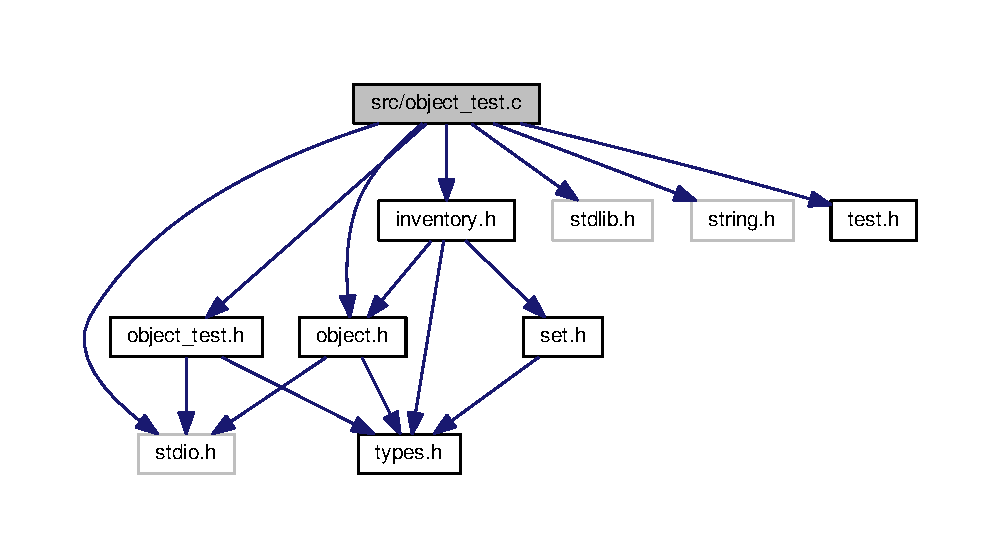
\includegraphics[width=350pt]{object__test_8c__incl}
\end{center}
\end{figure}
\subsection*{Macros}
\begin{DoxyCompactItemize}
\item 
\#define \hyperlink{object__test_8c_a2a77d2f2c5b698c69c19e1f8782bf709}{M\+A\+X\+\_\+\+T\+E\+S\+TS}~55
\end{DoxyCompactItemize}
\subsection*{Functions}
\begin{DoxyCompactItemize}
\item 
int \hyperlink{object__test_8c_a3c04138a5bfe5d72780bb7e82a18e627}{main} (int argc, char $\ast$$\ast$argv)
\begin{DoxyCompactList}\small\item\em Main function for object unit tests. \end{DoxyCompactList}\item 
void \hyperlink{object__test_8c_a3836d69f92ce7149d56bafcaec83f516}{test1\+\_\+object\+\_\+create} ()
\item 
void \hyperlink{object__test_8c_add54ab5e33a1b0a93e9ddcf73591bd9f}{test2\+\_\+object\+\_\+create} ()
\item 
void \hyperlink{object__test_8c_aa88e9e9dab92ba9c58851d7a7a8415f0}{test1\+\_\+object\+\_\+get\+\_\+id} ()
\item 
void \hyperlink{object__test_8c_a1ff250f0f43297f57fcce1f3a6ae490b}{test2\+\_\+object\+\_\+get\+\_\+id} ()
\item 
void \hyperlink{object__test_8c_ac62fbd4db0970e9942aa900a3ee2bba4}{test1\+\_\+object\+\_\+get\+\_\+location} ()
\item 
void \hyperlink{object__test_8c_aa8e3d1f2c80097572d9a453737d8cd44}{test2\+\_\+object\+\_\+get\+\_\+location} ()
\item 
void \hyperlink{object__test_8c_a74e25ad653c4a32b9922fff8e4f916fd}{test1\+\_\+object\+\_\+set\+\_\+name} ()
\item 
void \hyperlink{object__test_8c_acf42b7e7be91ede243f2aaa56c4c9347}{test2\+\_\+object\+\_\+set\+\_\+name} ()
\item 
void \hyperlink{object__test_8c_ab40669b5d083b6484197d917fb6882b1}{test3\+\_\+object\+\_\+set\+\_\+name} ()
\item 
void \hyperlink{object__test_8c_ad2411bc3cc47c9905e63a3d9c561d369}{test1\+\_\+object\+\_\+get\+\_\+name} ()
\item 
void \hyperlink{object__test_8c_abdfafbc7b8588d3dcdb05fd2beb2397e}{test2\+\_\+object\+\_\+get\+\_\+name} ()
\item 
void \hyperlink{object__test_8c_a364b4f750a8a99ee3edd8eace90766da}{test1\+\_\+object\+\_\+set\+\_\+original\+\_\+description} ()
\item 
void \hyperlink{object__test_8c_a9f99963e555263ceef814fec86db4758}{test2\+\_\+object\+\_\+set\+\_\+original\+\_\+description} ()
\item 
void \hyperlink{object__test_8c_a61b511105851e73fb0bdaf0b7624370b}{test3\+\_\+object\+\_\+set\+\_\+original\+\_\+description} ()
\item 
void \hyperlink{object__test_8c_a239d56f1aad1ab85ca1ed897abc98052}{test1\+\_\+object\+\_\+get\+\_\+original\+\_\+description} ()
\item 
void \hyperlink{object__test_8c_af05f0ac1f5b56dd4cd7bedf9f5170cda}{test2\+\_\+object\+\_\+get\+\_\+original\+\_\+description} ()
\item 
void \hyperlink{object__test_8c_a6f19ebf6034115c2cdcc3c7bfea25964}{test1\+\_\+object\+\_\+set\+\_\+id} ()
\item 
void \hyperlink{object__test_8c_a1f0cfd69428a6cf954fe37c9c21f8cb3}{test2\+\_\+object\+\_\+set\+\_\+id} ()
\item 
void \hyperlink{object__test_8c_aeed901e95aa669185059c85183e68a24}{test1\+\_\+object\+\_\+set\+\_\+location} ()
\item 
void \hyperlink{object__test_8c_a728404dd60089346883f325281e88f5f}{test1\+\_\+object\+\_\+get\+\_\+prop\+\_\+\+Movable} ()
\item 
void \hyperlink{object__test_8c_a2b377a9a92a83b71996a961426983bca}{test2\+\_\+object\+\_\+get\+\_\+prop\+\_\+\+Movable} ()
\item 
void \hyperlink{object__test_8c_a3c03468ba567762d74f481366784209d}{test1\+\_\+object\+\_\+set\+\_\+prop\+\_\+\+Movable} ()
\item 
void \hyperlink{object__test_8c_a90b53ff8f01a8c2c233af68f0e59cb82}{test2\+\_\+object\+\_\+set\+\_\+prop\+\_\+\+Movable} ()
\item 
void \hyperlink{object__test_8c_a8764a4a50a115de3c998d6ae53e8020e}{test3\+\_\+object\+\_\+set\+\_\+prop\+\_\+\+Movable} ()
\item 
void \hyperlink{object__test_8c_acc9f038ee43213c830877448b76ccfdf}{test1\+\_\+object\+\_\+get\+\_\+prop\+\_\+\+Moved} ()
\item 
void \hyperlink{object__test_8c_a6c5952b03a7737bb7b44ae4a63a8ff0b}{test2\+\_\+object\+\_\+get\+\_\+prop\+\_\+\+Moved} ()
\item 
void \hyperlink{object__test_8c_a04878b6ba45bdf63222c309bd97f6b65}{test1\+\_\+object\+\_\+set\+\_\+prop\+\_\+\+Moved} ()
\item 
void \hyperlink{object__test_8c_ab357bb60ef2e7c2c32aa8f5bf96dc7f0}{test2\+\_\+object\+\_\+set\+\_\+prop\+\_\+\+Moved} ()
\item 
void \hyperlink{object__test_8c_a7789238ee5681e10b4d49e6e9f457d40}{test3\+\_\+object\+\_\+set\+\_\+prop\+\_\+\+Moved} ()
\item 
void \hyperlink{object__test_8c_ae1755561dd25ae3c9826c095b081e4bb}{test1\+\_\+object\+\_\+get\+\_\+prop\+\_\+\+Hidden} ()
\item 
void \hyperlink{object__test_8c_a2aa1c98ca2de8aab36614e37217a0907}{test2\+\_\+object\+\_\+get\+\_\+prop\+\_\+\+Hidden} ()
\item 
void \hyperlink{object__test_8c_a3684b2ca710956aa6e61d26236497b34}{test1\+\_\+object\+\_\+set\+\_\+prop\+\_\+\+Hidden} ()
\item 
void \hyperlink{object__test_8c_a5f05b32f7e951027ca0fca90da4ae89e}{test2\+\_\+object\+\_\+set\+\_\+prop\+\_\+\+Hidden} ()
\item 
void \hyperlink{object__test_8c_a83a9139598c0d1683c39a390ce4af8ad}{test3\+\_\+object\+\_\+set\+\_\+prop\+\_\+\+Hidden} ()
\item 
void \hyperlink{object__test_8c_a40fbfa7d317b726cb6d02b23deb3914f}{test1\+\_\+object\+\_\+get\+\_\+prop\+\_\+\+Illuminate} ()
\item 
void \hyperlink{object__test_8c_a689e4149735a5543014921c1579950a1}{test2\+\_\+object\+\_\+get\+\_\+prop\+\_\+\+Illuminate} ()
\item 
void \hyperlink{object__test_8c_a31cda74045f4f4a7f222705974dcf6de}{test1\+\_\+object\+\_\+set\+\_\+prop\+\_\+\+Illuminate} ()
\item 
void \hyperlink{object__test_8c_afb0a0cc9ade8ecc2c15ae9e5697e7211}{test2\+\_\+object\+\_\+set\+\_\+prop\+\_\+\+Illuminate} ()
\item 
void \hyperlink{object__test_8c_aa6e6c87c5a7f2d3552dd33d7a5f160cf}{test3\+\_\+object\+\_\+set\+\_\+prop\+\_\+\+Illuminate} ()
\item 
void \hyperlink{object__test_8c_a02608a9321ba268814c20a67e8fbce27}{test1\+\_\+object\+\_\+get\+\_\+prop\+\_\+\+Switched\+On} ()
\item 
void \hyperlink{object__test_8c_a1a023ed883d17c1fd32b924548306cf4}{test2\+\_\+object\+\_\+get\+\_\+prop\+\_\+\+Switched\+On} ()
\item 
void \hyperlink{object__test_8c_a3a0e24b6614bcad78cc6025165d4ab87}{test1\+\_\+object\+\_\+set\+\_\+prop\+\_\+\+Switched\+On} ()
\item 
void \hyperlink{object__test_8c_a08c0ca2b1c356924ca66dcbb15d9e970}{test2\+\_\+object\+\_\+set\+\_\+prop\+\_\+\+Switched\+On} ()
\item 
void \hyperlink{object__test_8c_a404400e229425a94d3ef8c5d826ece78}{test3\+\_\+object\+\_\+set\+\_\+prop\+\_\+\+Switched\+On} ()
\item 
void \hyperlink{object__test_8c_a27e7bae76305733c1a8036bf54a4ff34}{test1\+\_\+object\+\_\+get\+\_\+prop\+\_\+\+Open} ()
\item 
void \hyperlink{object__test_8c_a300abd0f902e0c5865a1351dbb6e65c4}{test2\+\_\+object\+\_\+get\+\_\+prop\+\_\+\+Open} ()
\item 
void \hyperlink{object__test_8c_a353246fe61194086aea1ca9f94008d9a}{test1\+\_\+object\+\_\+set\+\_\+prop\+\_\+\+Open} ()
\item 
void \hyperlink{object__test_8c_a197746b5a031a7d4fda89035f22050f8}{test2\+\_\+object\+\_\+set\+\_\+prop\+\_\+\+Open} ()
\item 
void \hyperlink{object__test_8c_ae36abb53263ed855bde4dc2f47195813}{test3\+\_\+object\+\_\+set\+\_\+prop\+\_\+\+Open} ()
\item 
void \hyperlink{object__test_8c_ad36938109a07bb264f1005fe9ff5b118}{test1\+\_\+object\+\_\+get\+\_\+original\+\_\+position} ()
\item 
void \hyperlink{object__test_8c_a90212ac853f2702bcf7f83046f493810}{test2\+\_\+object\+\_\+get\+\_\+original\+\_\+position} ()
\item 
void \hyperlink{object__test_8c_aaef8c81d135b0e5dcc9972bc04991c69}{test3\+\_\+object\+\_\+get\+\_\+original\+\_\+position} ()
\item 
void \hyperlink{object__test_8c_af3fb1a489226895731af93b686741849}{test1\+\_\+object\+\_\+set\+\_\+original\+\_\+position} ()
\item 
void \hyperlink{object__test_8c_a64501207ceb4c2481bb45a334c71668f}{test2\+\_\+object\+\_\+set\+\_\+original\+\_\+position} ()
\item 
void \hyperlink{object__test_8c_a1a521d43a34ab0744c551f547120b24e}{test3\+\_\+object\+\_\+set\+\_\+original\+\_\+position} ()
\end{DoxyCompactItemize}


\subsection{Detailed Description}
It tests object module. 

\begin{DoxyAuthor}{Author}
Andres Mena 
\end{DoxyAuthor}
\begin{DoxyVersion}{Version}
1.\+0 
\end{DoxyVersion}
\begin{DoxyDate}{Date}
31-\/03-\/2018 
\end{DoxyDate}
\begin{DoxyCopyright}{Copyright}
G\+NU Public License 
\end{DoxyCopyright}


\subsection{Macro Definition Documentation}
\index{object\+\_\+test.\+c@{object\+\_\+test.\+c}!M\+A\+X\+\_\+\+T\+E\+S\+TS@{M\+A\+X\+\_\+\+T\+E\+S\+TS}}
\index{M\+A\+X\+\_\+\+T\+E\+S\+TS@{M\+A\+X\+\_\+\+T\+E\+S\+TS}!object\+\_\+test.\+c@{object\+\_\+test.\+c}}
\subsubsection[{\texorpdfstring{M\+A\+X\+\_\+\+T\+E\+S\+TS}{MAX_TESTS}}]{\setlength{\rightskip}{0pt plus 5cm}\#define M\+A\+X\+\_\+\+T\+E\+S\+TS~55}\hypertarget{object__test_8c_a2a77d2f2c5b698c69c19e1f8782bf709}{}\label{object__test_8c_a2a77d2f2c5b698c69c19e1f8782bf709}
Max amount of tests posible 

\subsection{Function Documentation}
\index{object\+\_\+test.\+c@{object\+\_\+test.\+c}!main@{main}}
\index{main@{main}!object\+\_\+test.\+c@{object\+\_\+test.\+c}}
\subsubsection[{\texorpdfstring{main(int argc, char $\ast$$\ast$argv)}{main(int argc, char **argv)}}]{\setlength{\rightskip}{0pt plus 5cm}int main (
\begin{DoxyParamCaption}
\item[{int}]{argc, }
\item[{char $\ast$$\ast$}]{argv}
\end{DoxyParamCaption}
)}\hypertarget{object__test_8c_a3c04138a5bfe5d72780bb7e82a18e627}{}\label{object__test_8c_a3c04138a5bfe5d72780bb7e82a18e627}


Main function for object unit tests. 

You may execute A\+LL or a S\+I\+N\+G\+LE test 1.-\/ No parameter -\/$>$ A\+LL test are executed 2.-\/ A number means a particular test (the one identified by that number) is executed \index{object\+\_\+test.\+c@{object\+\_\+test.\+c}!test1\+\_\+object\+\_\+create@{test1\+\_\+object\+\_\+create}}
\index{test1\+\_\+object\+\_\+create@{test1\+\_\+object\+\_\+create}!object\+\_\+test.\+c@{object\+\_\+test.\+c}}
\subsubsection[{\texorpdfstring{test1\+\_\+object\+\_\+create()}{test1_object_create()}}]{\setlength{\rightskip}{0pt plus 5cm}void test1\+\_\+object\+\_\+create (
\begin{DoxyParamCaption}
{}
\end{DoxyParamCaption}
)}\hypertarget{object__test_8c_a3836d69f92ce7149d56bafcaec83f516}{}\label{object__test_8c_a3836d69f92ce7149d56bafcaec83f516}
\begin{DoxyRefDesc}{Test}
\item[\hyperlink{test__test000050}{Test}]Test object creation \end{DoxyRefDesc}
\begin{DoxyPrecond}{Precondition}
object ID 
\end{DoxyPrecond}
\begin{DoxyPostcond}{Postcondition}
Non N\+U\+LL pointer to object 
\end{DoxyPostcond}
\index{object\+\_\+test.\+c@{object\+\_\+test.\+c}!test1\+\_\+object\+\_\+get\+\_\+id@{test1\+\_\+object\+\_\+get\+\_\+id}}
\index{test1\+\_\+object\+\_\+get\+\_\+id@{test1\+\_\+object\+\_\+get\+\_\+id}!object\+\_\+test.\+c@{object\+\_\+test.\+c}}
\subsubsection[{\texorpdfstring{test1\+\_\+object\+\_\+get\+\_\+id()}{test1_object_get_id()}}]{\setlength{\rightskip}{0pt plus 5cm}void test1\+\_\+object\+\_\+get\+\_\+id (
\begin{DoxyParamCaption}
{}
\end{DoxyParamCaption}
)}\hypertarget{object__test_8c_aa88e9e9dab92ba9c58851d7a7a8415f0}{}\label{object__test_8c_aa88e9e9dab92ba9c58851d7a7a8415f0}
\begin{DoxyRefDesc}{Test}
\item[\hyperlink{test__test000052}{Test}]Test obtaining id of object \end{DoxyRefDesc}
\begin{DoxyPrecond}{Precondition}
Object pointer N\+U\+LL 
\end{DoxyPrecond}
\begin{DoxyPostcond}{Postcondition}
N\+O\+\_\+\+ID 
\end{DoxyPostcond}
\index{object\+\_\+test.\+c@{object\+\_\+test.\+c}!test1\+\_\+object\+\_\+get\+\_\+location@{test1\+\_\+object\+\_\+get\+\_\+location}}
\index{test1\+\_\+object\+\_\+get\+\_\+location@{test1\+\_\+object\+\_\+get\+\_\+location}!object\+\_\+test.\+c@{object\+\_\+test.\+c}}
\subsubsection[{\texorpdfstring{test1\+\_\+object\+\_\+get\+\_\+location()}{test1_object_get_location()}}]{\setlength{\rightskip}{0pt plus 5cm}void test1\+\_\+object\+\_\+get\+\_\+location (
\begin{DoxyParamCaption}
{}
\end{DoxyParamCaption}
)}\hypertarget{object__test_8c_ac62fbd4db0970e9942aa900a3ee2bba4}{}\label{object__test_8c_ac62fbd4db0970e9942aa900a3ee2bba4}
\begin{DoxyRefDesc}{Test}
\item[\hyperlink{test__test000054}{Test}]Test obtaining location of object \end{DoxyRefDesc}
\begin{DoxyPrecond}{Precondition}
Object pointer N\+U\+LL 
\end{DoxyPrecond}
\begin{DoxyPostcond}{Postcondition}
N\+O\+\_\+\+ID 
\end{DoxyPostcond}
\index{object\+\_\+test.\+c@{object\+\_\+test.\+c}!test1\+\_\+object\+\_\+get\+\_\+name@{test1\+\_\+object\+\_\+get\+\_\+name}}
\index{test1\+\_\+object\+\_\+get\+\_\+name@{test1\+\_\+object\+\_\+get\+\_\+name}!object\+\_\+test.\+c@{object\+\_\+test.\+c}}
\subsubsection[{\texorpdfstring{test1\+\_\+object\+\_\+get\+\_\+name()}{test1_object_get_name()}}]{\setlength{\rightskip}{0pt plus 5cm}void test1\+\_\+object\+\_\+get\+\_\+name (
\begin{DoxyParamCaption}
{}
\end{DoxyParamCaption}
)}\hypertarget{object__test_8c_ad2411bc3cc47c9905e63a3d9c561d369}{}\label{object__test_8c_ad2411bc3cc47c9905e63a3d9c561d369}
\begin{DoxyRefDesc}{Test}
\item[\hyperlink{test__test000059}{Test}]Test function for object\+\_\+name obtaining \end{DoxyRefDesc}
\begin{DoxyPrecond}{Precondition}
Object pointer 
\end{DoxyPrecond}
\begin{DoxyPostcond}{Postcondition}
string of characters (previously added) 
\end{DoxyPostcond}
\index{object\+\_\+test.\+c@{object\+\_\+test.\+c}!test1\+\_\+object\+\_\+get\+\_\+original\+\_\+description@{test1\+\_\+object\+\_\+get\+\_\+original\+\_\+description}}
\index{test1\+\_\+object\+\_\+get\+\_\+original\+\_\+description@{test1\+\_\+object\+\_\+get\+\_\+original\+\_\+description}!object\+\_\+test.\+c@{object\+\_\+test.\+c}}
\subsubsection[{\texorpdfstring{test1\+\_\+object\+\_\+get\+\_\+original\+\_\+description()}{test1_object_get_original_description()}}]{\setlength{\rightskip}{0pt plus 5cm}void test1\+\_\+object\+\_\+get\+\_\+original\+\_\+description (
\begin{DoxyParamCaption}
{}
\end{DoxyParamCaption}
)}\hypertarget{object__test_8c_a239d56f1aad1ab85ca1ed897abc98052}{}\label{object__test_8c_a239d56f1aad1ab85ca1ed897abc98052}
\begin{DoxyRefDesc}{Test}
\item[\hyperlink{test__test000064}{Test}]Test function for description of object obtaining \end{DoxyRefDesc}
\begin{DoxyPrecond}{Precondition}
Object pointer 
\end{DoxyPrecond}
\begin{DoxyPostcond}{Postcondition}
String with name 
\end{DoxyPostcond}
\index{object\+\_\+test.\+c@{object\+\_\+test.\+c}!test1\+\_\+object\+\_\+get\+\_\+original\+\_\+position@{test1\+\_\+object\+\_\+get\+\_\+original\+\_\+position}}
\index{test1\+\_\+object\+\_\+get\+\_\+original\+\_\+position@{test1\+\_\+object\+\_\+get\+\_\+original\+\_\+position}!object\+\_\+test.\+c@{object\+\_\+test.\+c}}
\subsubsection[{\texorpdfstring{test1\+\_\+object\+\_\+get\+\_\+original\+\_\+position()}{test1_object_get_original_position()}}]{\setlength{\rightskip}{0pt plus 5cm}void test1\+\_\+object\+\_\+get\+\_\+original\+\_\+position (
\begin{DoxyParamCaption}
{}
\end{DoxyParamCaption}
)}\hypertarget{object__test_8c_ad36938109a07bb264f1005fe9ff5b118}{}\label{object__test_8c_ad36938109a07bb264f1005fe9ff5b118}
\begin{DoxyRefDesc}{Test}
\item[\hyperlink{test__test000094}{Test}]Test getting original position of object \end{DoxyRefDesc}
\begin{DoxyPrecond}{Precondition}
Object pointer 
\end{DoxyPrecond}
\begin{DoxyPostcond}{Postcondition}
N\+O\+\_\+\+ID 
\end{DoxyPostcond}
\index{object\+\_\+test.\+c@{object\+\_\+test.\+c}!test1\+\_\+object\+\_\+get\+\_\+prop\+\_\+\+Hidden@{test1\+\_\+object\+\_\+get\+\_\+prop\+\_\+\+Hidden}}
\index{test1\+\_\+object\+\_\+get\+\_\+prop\+\_\+\+Hidden@{test1\+\_\+object\+\_\+get\+\_\+prop\+\_\+\+Hidden}!object\+\_\+test.\+c@{object\+\_\+test.\+c}}
\subsubsection[{\texorpdfstring{test1\+\_\+object\+\_\+get\+\_\+prop\+\_\+\+Hidden()}{test1_object_get_prop_Hidden()}}]{\setlength{\rightskip}{0pt plus 5cm}void test1\+\_\+object\+\_\+get\+\_\+prop\+\_\+\+Hidden (
\begin{DoxyParamCaption}
{}
\end{DoxyParamCaption}
)}\hypertarget{object__test_8c_ae1755561dd25ae3c9826c095b081e4bb}{}\label{object__test_8c_ae1755561dd25ae3c9826c095b081e4bb}
\begin{DoxyRefDesc}{Test}
\item[\hyperlink{test__test000100}{Test}]Test obtaining property Hidden of object \end{DoxyRefDesc}
\begin{DoxyPrecond}{Precondition}
Object pointer 
\end{DoxyPrecond}
\begin{DoxyPostcond}{Postcondition}
F\+A\+L\+SE property 
\end{DoxyPostcond}
\index{object\+\_\+test.\+c@{object\+\_\+test.\+c}!test1\+\_\+object\+\_\+get\+\_\+prop\+\_\+\+Illuminate@{test1\+\_\+object\+\_\+get\+\_\+prop\+\_\+\+Illuminate}}
\index{test1\+\_\+object\+\_\+get\+\_\+prop\+\_\+\+Illuminate@{test1\+\_\+object\+\_\+get\+\_\+prop\+\_\+\+Illuminate}!object\+\_\+test.\+c@{object\+\_\+test.\+c}}
\subsubsection[{\texorpdfstring{test1\+\_\+object\+\_\+get\+\_\+prop\+\_\+\+Illuminate()}{test1_object_get_prop_Illuminate()}}]{\setlength{\rightskip}{0pt plus 5cm}void test1\+\_\+object\+\_\+get\+\_\+prop\+\_\+\+Illuminate (
\begin{DoxyParamCaption}
{}
\end{DoxyParamCaption}
)}\hypertarget{object__test_8c_a40fbfa7d317b726cb6d02b23deb3914f}{}\label{object__test_8c_a40fbfa7d317b726cb6d02b23deb3914f}
\begin{DoxyRefDesc}{Test}
\item[\hyperlink{test__test000079}{Test}]Test obtaining property illuminate of object \end{DoxyRefDesc}
\begin{DoxyPrecond}{Precondition}
Object pointer 
\end{DoxyPrecond}
\begin{DoxyPostcond}{Postcondition}
F\+A\+L\+SE property 
\end{DoxyPostcond}
\index{object\+\_\+test.\+c@{object\+\_\+test.\+c}!test1\+\_\+object\+\_\+get\+\_\+prop\+\_\+\+Movable@{test1\+\_\+object\+\_\+get\+\_\+prop\+\_\+\+Movable}}
\index{test1\+\_\+object\+\_\+get\+\_\+prop\+\_\+\+Movable@{test1\+\_\+object\+\_\+get\+\_\+prop\+\_\+\+Movable}!object\+\_\+test.\+c@{object\+\_\+test.\+c}}
\subsubsection[{\texorpdfstring{test1\+\_\+object\+\_\+get\+\_\+prop\+\_\+\+Movable()}{test1_object_get_prop_Movable()}}]{\setlength{\rightskip}{0pt plus 5cm}void test1\+\_\+object\+\_\+get\+\_\+prop\+\_\+\+Movable (
\begin{DoxyParamCaption}
{}
\end{DoxyParamCaption}
)}\hypertarget{object__test_8c_a728404dd60089346883f325281e88f5f}{}\label{object__test_8c_a728404dd60089346883f325281e88f5f}
\begin{DoxyRefDesc}{Test}
\item[\hyperlink{test__test000069}{Test}]Test obtaining property movable of object \end{DoxyRefDesc}
\begin{DoxyPrecond}{Precondition}
Object pointer 
\end{DoxyPrecond}
\begin{DoxyPostcond}{Postcondition}
F\+A\+L\+SE property 
\end{DoxyPostcond}
\index{object\+\_\+test.\+c@{object\+\_\+test.\+c}!test1\+\_\+object\+\_\+get\+\_\+prop\+\_\+\+Moved@{test1\+\_\+object\+\_\+get\+\_\+prop\+\_\+\+Moved}}
\index{test1\+\_\+object\+\_\+get\+\_\+prop\+\_\+\+Moved@{test1\+\_\+object\+\_\+get\+\_\+prop\+\_\+\+Moved}!object\+\_\+test.\+c@{object\+\_\+test.\+c}}
\subsubsection[{\texorpdfstring{test1\+\_\+object\+\_\+get\+\_\+prop\+\_\+\+Moved()}{test1_object_get_prop_Moved()}}]{\setlength{\rightskip}{0pt plus 5cm}void test1\+\_\+object\+\_\+get\+\_\+prop\+\_\+\+Moved (
\begin{DoxyParamCaption}
{}
\end{DoxyParamCaption}
)}\hypertarget{object__test_8c_acc9f038ee43213c830877448b76ccfdf}{}\label{object__test_8c_acc9f038ee43213c830877448b76ccfdf}
\begin{DoxyRefDesc}{Test}
\item[\hyperlink{test__test000074}{Test}]Test obtaining property moved of object \end{DoxyRefDesc}
\begin{DoxyPrecond}{Precondition}
Object pointer 
\end{DoxyPrecond}
\begin{DoxyPostcond}{Postcondition}
F\+A\+L\+SE property 
\end{DoxyPostcond}
\index{object\+\_\+test.\+c@{object\+\_\+test.\+c}!test1\+\_\+object\+\_\+get\+\_\+prop\+\_\+\+Open@{test1\+\_\+object\+\_\+get\+\_\+prop\+\_\+\+Open}}
\index{test1\+\_\+object\+\_\+get\+\_\+prop\+\_\+\+Open@{test1\+\_\+object\+\_\+get\+\_\+prop\+\_\+\+Open}!object\+\_\+test.\+c@{object\+\_\+test.\+c}}
\subsubsection[{\texorpdfstring{test1\+\_\+object\+\_\+get\+\_\+prop\+\_\+\+Open()}{test1_object_get_prop_Open()}}]{\setlength{\rightskip}{0pt plus 5cm}void test1\+\_\+object\+\_\+get\+\_\+prop\+\_\+\+Open (
\begin{DoxyParamCaption}
{}
\end{DoxyParamCaption}
)}\hypertarget{object__test_8c_a27e7bae76305733c1a8036bf54a4ff34}{}\label{object__test_8c_a27e7bae76305733c1a8036bf54a4ff34}
\begin{DoxyRefDesc}{Test}
\item[\hyperlink{test__test000089}{Test}]Test getting property open of object \end{DoxyRefDesc}
\begin{DoxyPrecond}{Precondition}
Object pointer 
\end{DoxyPrecond}
\begin{DoxyPostcond}{Postcondition}
N\+O\+\_\+\+ID 
\end{DoxyPostcond}
\index{object\+\_\+test.\+c@{object\+\_\+test.\+c}!test1\+\_\+object\+\_\+get\+\_\+prop\+\_\+\+Switched\+On@{test1\+\_\+object\+\_\+get\+\_\+prop\+\_\+\+Switched\+On}}
\index{test1\+\_\+object\+\_\+get\+\_\+prop\+\_\+\+Switched\+On@{test1\+\_\+object\+\_\+get\+\_\+prop\+\_\+\+Switched\+On}!object\+\_\+test.\+c@{object\+\_\+test.\+c}}
\subsubsection[{\texorpdfstring{test1\+\_\+object\+\_\+get\+\_\+prop\+\_\+\+Switched\+On()}{test1_object_get_prop_SwitchedOn()}}]{\setlength{\rightskip}{0pt plus 5cm}void test1\+\_\+object\+\_\+get\+\_\+prop\+\_\+\+Switched\+On (
\begin{DoxyParamCaption}
{}
\end{DoxyParamCaption}
)}\hypertarget{object__test_8c_a02608a9321ba268814c20a67e8fbce27}{}\label{object__test_8c_a02608a9321ba268814c20a67e8fbce27}
\begin{DoxyRefDesc}{Test}
\item[\hyperlink{test__test000084}{Test}]Test obtaining property switchedon of object \end{DoxyRefDesc}
\begin{DoxyPrecond}{Precondition}
Object pointer 
\end{DoxyPrecond}
\begin{DoxyPostcond}{Postcondition}
F\+A\+L\+SE property 
\end{DoxyPostcond}
\index{object\+\_\+test.\+c@{object\+\_\+test.\+c}!test1\+\_\+object\+\_\+set\+\_\+id@{test1\+\_\+object\+\_\+set\+\_\+id}}
\index{test1\+\_\+object\+\_\+set\+\_\+id@{test1\+\_\+object\+\_\+set\+\_\+id}!object\+\_\+test.\+c@{object\+\_\+test.\+c}}
\subsubsection[{\texorpdfstring{test1\+\_\+object\+\_\+set\+\_\+id()}{test1_object_set_id()}}]{\setlength{\rightskip}{0pt plus 5cm}void test1\+\_\+object\+\_\+set\+\_\+id (
\begin{DoxyParamCaption}
{}
\end{DoxyParamCaption}
)}\hypertarget{object__test_8c_a6f19ebf6034115c2cdcc3c7bfea25964}{}\label{object__test_8c_a6f19ebf6034115c2cdcc3c7bfea25964}
\begin{DoxyRefDesc}{Test}
\item[\hyperlink{test__test000066}{Test}]Test obtaining id of object \end{DoxyRefDesc}
\begin{DoxyPrecond}{Precondition}
Object pointer (with object id) 
\end{DoxyPrecond}
\begin{DoxyPostcond}{Postcondition}
Id of object 
\end{DoxyPostcond}
\index{object\+\_\+test.\+c@{object\+\_\+test.\+c}!test1\+\_\+object\+\_\+set\+\_\+location@{test1\+\_\+object\+\_\+set\+\_\+location}}
\index{test1\+\_\+object\+\_\+set\+\_\+location@{test1\+\_\+object\+\_\+set\+\_\+location}!object\+\_\+test.\+c@{object\+\_\+test.\+c}}
\subsubsection[{\texorpdfstring{test1\+\_\+object\+\_\+set\+\_\+location()}{test1_object_set_location()}}]{\setlength{\rightskip}{0pt plus 5cm}void test1\+\_\+object\+\_\+set\+\_\+location (
\begin{DoxyParamCaption}
{}
\end{DoxyParamCaption}
)}\hypertarget{object__test_8c_aeed901e95aa669185059c85183e68a24}{}\label{object__test_8c_aeed901e95aa669185059c85183e68a24}
\begin{DoxyRefDesc}{Test}
\item[\hyperlink{test__test000068}{Test}]Test obtaining location of object \end{DoxyRefDesc}
\begin{DoxyPrecond}{Precondition}
Object pointer with object added 
\end{DoxyPrecond}
\begin{DoxyPostcond}{Postcondition}
object location == location sent 
\end{DoxyPostcond}
\index{object\+\_\+test.\+c@{object\+\_\+test.\+c}!test1\+\_\+object\+\_\+set\+\_\+name@{test1\+\_\+object\+\_\+set\+\_\+name}}
\index{test1\+\_\+object\+\_\+set\+\_\+name@{test1\+\_\+object\+\_\+set\+\_\+name}!object\+\_\+test.\+c@{object\+\_\+test.\+c}}
\subsubsection[{\texorpdfstring{test1\+\_\+object\+\_\+set\+\_\+name()}{test1_object_set_name()}}]{\setlength{\rightskip}{0pt plus 5cm}void test1\+\_\+object\+\_\+set\+\_\+name (
\begin{DoxyParamCaption}
{}
\end{DoxyParamCaption}
)}\hypertarget{object__test_8c_a74e25ad653c4a32b9922fff8e4f916fd}{}\label{object__test_8c_a74e25ad653c4a32b9922fff8e4f916fd}
\begin{DoxyRefDesc}{Test}
\item[\hyperlink{test__test000056}{Test}]Test function object\+\_\+name setting \end{DoxyRefDesc}
\begin{DoxyPrecond}{Precondition}
String with space name and Object pointer 
\end{DoxyPrecond}
\begin{DoxyPostcond}{Postcondition}
Ouput==OK 
\end{DoxyPostcond}
\index{object\+\_\+test.\+c@{object\+\_\+test.\+c}!test1\+\_\+object\+\_\+set\+\_\+original\+\_\+description@{test1\+\_\+object\+\_\+set\+\_\+original\+\_\+description}}
\index{test1\+\_\+object\+\_\+set\+\_\+original\+\_\+description@{test1\+\_\+object\+\_\+set\+\_\+original\+\_\+description}!object\+\_\+test.\+c@{object\+\_\+test.\+c}}
\subsubsection[{\texorpdfstring{test1\+\_\+object\+\_\+set\+\_\+original\+\_\+description()}{test1_object_set_original_description()}}]{\setlength{\rightskip}{0pt plus 5cm}void test1\+\_\+object\+\_\+set\+\_\+original\+\_\+description (
\begin{DoxyParamCaption}
{}
\end{DoxyParamCaption}
)}\hypertarget{object__test_8c_a364b4f750a8a99ee3edd8eace90766da}{}\label{object__test_8c_a364b4f750a8a99ee3edd8eace90766da}
\begin{DoxyRefDesc}{Test}
\item[\hyperlink{test__test000061}{Test}]Test function for description of object setting \end{DoxyRefDesc}
\begin{DoxyPrecond}{Precondition}
String of characters and Object pointer 
\end{DoxyPrecond}
\begin{DoxyPostcond}{Postcondition}
S\+T\+A\+T\+US=OK 
\end{DoxyPostcond}
\index{object\+\_\+test.\+c@{object\+\_\+test.\+c}!test1\+\_\+object\+\_\+set\+\_\+original\+\_\+position@{test1\+\_\+object\+\_\+set\+\_\+original\+\_\+position}}
\index{test1\+\_\+object\+\_\+set\+\_\+original\+\_\+position@{test1\+\_\+object\+\_\+set\+\_\+original\+\_\+position}!object\+\_\+test.\+c@{object\+\_\+test.\+c}}
\subsubsection[{\texorpdfstring{test1\+\_\+object\+\_\+set\+\_\+original\+\_\+position()}{test1_object_set_original_position()}}]{\setlength{\rightskip}{0pt plus 5cm}void test1\+\_\+object\+\_\+set\+\_\+original\+\_\+position (
\begin{DoxyParamCaption}
{}
\end{DoxyParamCaption}
)}\hypertarget{object__test_8c_af3fb1a489226895731af93b686741849}{}\label{object__test_8c_af3fb1a489226895731af93b686741849}
\begin{DoxyRefDesc}{Test}
\item[\hyperlink{test__test000097}{Test}]Test setting original position of object \end{DoxyRefDesc}
\begin{DoxyPrecond}{Precondition}
Object pointer with a position 
\end{DoxyPrecond}
\begin{DoxyPostcond}{Postcondition}
Position introduced previously 
\end{DoxyPostcond}
\index{object\+\_\+test.\+c@{object\+\_\+test.\+c}!test1\+\_\+object\+\_\+set\+\_\+prop\+\_\+\+Hidden@{test1\+\_\+object\+\_\+set\+\_\+prop\+\_\+\+Hidden}}
\index{test1\+\_\+object\+\_\+set\+\_\+prop\+\_\+\+Hidden@{test1\+\_\+object\+\_\+set\+\_\+prop\+\_\+\+Hidden}!object\+\_\+test.\+c@{object\+\_\+test.\+c}}
\subsubsection[{\texorpdfstring{test1\+\_\+object\+\_\+set\+\_\+prop\+\_\+\+Hidden()}{test1_object_set_prop_Hidden()}}]{\setlength{\rightskip}{0pt plus 5cm}void test1\+\_\+object\+\_\+set\+\_\+prop\+\_\+\+Hidden (
\begin{DoxyParamCaption}
{}
\end{DoxyParamCaption}
)}\hypertarget{object__test_8c_a3684b2ca710956aa6e61d26236497b34}{}\label{object__test_8c_a3684b2ca710956aa6e61d26236497b34}
\begin{DoxyRefDesc}{Test}
\item[\hyperlink{test__test000102}{Test}]Test setting property Hidden of object \end{DoxyRefDesc}
\begin{DoxyPrecond}{Precondition}
Object pointer and T\+R\+UE boolean 
\end{DoxyPrecond}
\begin{DoxyPostcond}{Postcondition}
T\+R\+UE property 
\end{DoxyPostcond}
\index{object\+\_\+test.\+c@{object\+\_\+test.\+c}!test1\+\_\+object\+\_\+set\+\_\+prop\+\_\+\+Illuminate@{test1\+\_\+object\+\_\+set\+\_\+prop\+\_\+\+Illuminate}}
\index{test1\+\_\+object\+\_\+set\+\_\+prop\+\_\+\+Illuminate@{test1\+\_\+object\+\_\+set\+\_\+prop\+\_\+\+Illuminate}!object\+\_\+test.\+c@{object\+\_\+test.\+c}}
\subsubsection[{\texorpdfstring{test1\+\_\+object\+\_\+set\+\_\+prop\+\_\+\+Illuminate()}{test1_object_set_prop_Illuminate()}}]{\setlength{\rightskip}{0pt plus 5cm}void test1\+\_\+object\+\_\+set\+\_\+prop\+\_\+\+Illuminate (
\begin{DoxyParamCaption}
{}
\end{DoxyParamCaption}
)}\hypertarget{object__test_8c_a31cda74045f4f4a7f222705974dcf6de}{}\label{object__test_8c_a31cda74045f4f4a7f222705974dcf6de}
\begin{DoxyRefDesc}{Test}
\item[\hyperlink{test__test000081}{Test}]Test setting property illuminate of object \end{DoxyRefDesc}
\begin{DoxyPrecond}{Precondition}
Object pointer and T\+R\+UE boolean 
\end{DoxyPrecond}
\begin{DoxyPostcond}{Postcondition}
T\+R\+UE property 
\end{DoxyPostcond}
\index{object\+\_\+test.\+c@{object\+\_\+test.\+c}!test1\+\_\+object\+\_\+set\+\_\+prop\+\_\+\+Movable@{test1\+\_\+object\+\_\+set\+\_\+prop\+\_\+\+Movable}}
\index{test1\+\_\+object\+\_\+set\+\_\+prop\+\_\+\+Movable@{test1\+\_\+object\+\_\+set\+\_\+prop\+\_\+\+Movable}!object\+\_\+test.\+c@{object\+\_\+test.\+c}}
\subsubsection[{\texorpdfstring{test1\+\_\+object\+\_\+set\+\_\+prop\+\_\+\+Movable()}{test1_object_set_prop_Movable()}}]{\setlength{\rightskip}{0pt plus 5cm}void test1\+\_\+object\+\_\+set\+\_\+prop\+\_\+\+Movable (
\begin{DoxyParamCaption}
{}
\end{DoxyParamCaption}
)}\hypertarget{object__test_8c_a3c03468ba567762d74f481366784209d}{}\label{object__test_8c_a3c03468ba567762d74f481366784209d}
\begin{DoxyRefDesc}{Test}
\item[\hyperlink{test__test000071}{Test}]Test setting property movable of object \end{DoxyRefDesc}
\begin{DoxyPrecond}{Precondition}
Object pointer and T\+R\+UE boolean 
\end{DoxyPrecond}
\begin{DoxyPostcond}{Postcondition}
T\+R\+UE property 
\end{DoxyPostcond}
\index{object\+\_\+test.\+c@{object\+\_\+test.\+c}!test1\+\_\+object\+\_\+set\+\_\+prop\+\_\+\+Moved@{test1\+\_\+object\+\_\+set\+\_\+prop\+\_\+\+Moved}}
\index{test1\+\_\+object\+\_\+set\+\_\+prop\+\_\+\+Moved@{test1\+\_\+object\+\_\+set\+\_\+prop\+\_\+\+Moved}!object\+\_\+test.\+c@{object\+\_\+test.\+c}}
\subsubsection[{\texorpdfstring{test1\+\_\+object\+\_\+set\+\_\+prop\+\_\+\+Moved()}{test1_object_set_prop_Moved()}}]{\setlength{\rightskip}{0pt plus 5cm}void test1\+\_\+object\+\_\+set\+\_\+prop\+\_\+\+Moved (
\begin{DoxyParamCaption}
{}
\end{DoxyParamCaption}
)}\hypertarget{object__test_8c_a04878b6ba45bdf63222c309bd97f6b65}{}\label{object__test_8c_a04878b6ba45bdf63222c309bd97f6b65}
\begin{DoxyRefDesc}{Test}
\item[\hyperlink{test__test000076}{Test}]Test setting property moved of object \end{DoxyRefDesc}
\begin{DoxyPrecond}{Precondition}
Object pointer and T\+R\+UE boolean 
\end{DoxyPrecond}
\begin{DoxyPostcond}{Postcondition}
T\+R\+UE property 
\end{DoxyPostcond}
\index{object\+\_\+test.\+c@{object\+\_\+test.\+c}!test1\+\_\+object\+\_\+set\+\_\+prop\+\_\+\+Open@{test1\+\_\+object\+\_\+set\+\_\+prop\+\_\+\+Open}}
\index{test1\+\_\+object\+\_\+set\+\_\+prop\+\_\+\+Open@{test1\+\_\+object\+\_\+set\+\_\+prop\+\_\+\+Open}!object\+\_\+test.\+c@{object\+\_\+test.\+c}}
\subsubsection[{\texorpdfstring{test1\+\_\+object\+\_\+set\+\_\+prop\+\_\+\+Open()}{test1_object_set_prop_Open()}}]{\setlength{\rightskip}{0pt plus 5cm}void test1\+\_\+object\+\_\+set\+\_\+prop\+\_\+\+Open (
\begin{DoxyParamCaption}
{}
\end{DoxyParamCaption}
)}\hypertarget{object__test_8c_a353246fe61194086aea1ca9f94008d9a}{}\label{object__test_8c_a353246fe61194086aea1ca9f94008d9a}
\begin{DoxyRefDesc}{Test}
\item[\hyperlink{test__test000091}{Test}]Test setting property open of object \end{DoxyRefDesc}
\begin{DoxyPrecond}{Precondition}
Object pointer and ID 
\end{DoxyPrecond}
\begin{DoxyPostcond}{Postcondition}
ID previously introduced 
\end{DoxyPostcond}
\index{object\+\_\+test.\+c@{object\+\_\+test.\+c}!test1\+\_\+object\+\_\+set\+\_\+prop\+\_\+\+Switched\+On@{test1\+\_\+object\+\_\+set\+\_\+prop\+\_\+\+Switched\+On}}
\index{test1\+\_\+object\+\_\+set\+\_\+prop\+\_\+\+Switched\+On@{test1\+\_\+object\+\_\+set\+\_\+prop\+\_\+\+Switched\+On}!object\+\_\+test.\+c@{object\+\_\+test.\+c}}
\subsubsection[{\texorpdfstring{test1\+\_\+object\+\_\+set\+\_\+prop\+\_\+\+Switched\+On()}{test1_object_set_prop_SwitchedOn()}}]{\setlength{\rightskip}{0pt plus 5cm}void test1\+\_\+object\+\_\+set\+\_\+prop\+\_\+\+Switched\+On (
\begin{DoxyParamCaption}
{}
\end{DoxyParamCaption}
)}\hypertarget{object__test_8c_a3a0e24b6614bcad78cc6025165d4ab87}{}\label{object__test_8c_a3a0e24b6614bcad78cc6025165d4ab87}
\begin{DoxyRefDesc}{Test}
\item[\hyperlink{test__test000086}{Test}]Test setting property switchedon of object \end{DoxyRefDesc}
\begin{DoxyPrecond}{Precondition}
Object pointer and T\+R\+UE boolean 
\end{DoxyPrecond}
\begin{DoxyPostcond}{Postcondition}
T\+R\+UE property 
\end{DoxyPostcond}
\index{object\+\_\+test.\+c@{object\+\_\+test.\+c}!test2\+\_\+object\+\_\+create@{test2\+\_\+object\+\_\+create}}
\index{test2\+\_\+object\+\_\+create@{test2\+\_\+object\+\_\+create}!object\+\_\+test.\+c@{object\+\_\+test.\+c}}
\subsubsection[{\texorpdfstring{test2\+\_\+object\+\_\+create()}{test2_object_create()}}]{\setlength{\rightskip}{0pt plus 5cm}void test2\+\_\+object\+\_\+create (
\begin{DoxyParamCaption}
{}
\end{DoxyParamCaption}
)}\hypertarget{object__test_8c_add54ab5e33a1b0a93e9ddcf73591bd9f}{}\label{object__test_8c_add54ab5e33a1b0a93e9ddcf73591bd9f}
\begin{DoxyRefDesc}{Test}
\item[\hyperlink{test__test000051}{Test}]Test object creation \end{DoxyRefDesc}
\begin{DoxyPrecond}{Precondition}
object ID 
\end{DoxyPrecond}
\begin{DoxyPostcond}{Postcondition}
Object\+\_\+\+ID == Supplied Object Id 
\end{DoxyPostcond}
\index{object\+\_\+test.\+c@{object\+\_\+test.\+c}!test2\+\_\+object\+\_\+get\+\_\+id@{test2\+\_\+object\+\_\+get\+\_\+id}}
\index{test2\+\_\+object\+\_\+get\+\_\+id@{test2\+\_\+object\+\_\+get\+\_\+id}!object\+\_\+test.\+c@{object\+\_\+test.\+c}}
\subsubsection[{\texorpdfstring{test2\+\_\+object\+\_\+get\+\_\+id()}{test2_object_get_id()}}]{\setlength{\rightskip}{0pt plus 5cm}void test2\+\_\+object\+\_\+get\+\_\+id (
\begin{DoxyParamCaption}
{}
\end{DoxyParamCaption}
)}\hypertarget{object__test_8c_a1ff250f0f43297f57fcce1f3a6ae490b}{}\label{object__test_8c_a1ff250f0f43297f57fcce1f3a6ae490b}
\begin{DoxyRefDesc}{Test}
\item[\hyperlink{test__test000053}{Test}]Test obtaining id of object \end{DoxyRefDesc}
\begin{DoxyPrecond}{Precondition}
Object pointer 
\end{DoxyPrecond}
\begin{DoxyPostcond}{Postcondition}
id of the object 
\end{DoxyPostcond}
\index{object\+\_\+test.\+c@{object\+\_\+test.\+c}!test2\+\_\+object\+\_\+get\+\_\+location@{test2\+\_\+object\+\_\+get\+\_\+location}}
\index{test2\+\_\+object\+\_\+get\+\_\+location@{test2\+\_\+object\+\_\+get\+\_\+location}!object\+\_\+test.\+c@{object\+\_\+test.\+c}}
\subsubsection[{\texorpdfstring{test2\+\_\+object\+\_\+get\+\_\+location()}{test2_object_get_location()}}]{\setlength{\rightskip}{0pt plus 5cm}void test2\+\_\+object\+\_\+get\+\_\+location (
\begin{DoxyParamCaption}
{}
\end{DoxyParamCaption}
)}\hypertarget{object__test_8c_aa8e3d1f2c80097572d9a453737d8cd44}{}\label{object__test_8c_aa8e3d1f2c80097572d9a453737d8cd44}
\begin{DoxyRefDesc}{Test}
\item[\hyperlink{test__test000055}{Test}]Test obtaining location of object \end{DoxyRefDesc}
\begin{DoxyPrecond}{Precondition}
Object pointer 
\end{DoxyPrecond}
\begin{DoxyPostcond}{Postcondition}
id of object previously added 
\end{DoxyPostcond}
\index{object\+\_\+test.\+c@{object\+\_\+test.\+c}!test2\+\_\+object\+\_\+get\+\_\+name@{test2\+\_\+object\+\_\+get\+\_\+name}}
\index{test2\+\_\+object\+\_\+get\+\_\+name@{test2\+\_\+object\+\_\+get\+\_\+name}!object\+\_\+test.\+c@{object\+\_\+test.\+c}}
\subsubsection[{\texorpdfstring{test2\+\_\+object\+\_\+get\+\_\+name()}{test2_object_get_name()}}]{\setlength{\rightskip}{0pt plus 5cm}void test2\+\_\+object\+\_\+get\+\_\+name (
\begin{DoxyParamCaption}
{}
\end{DoxyParamCaption}
)}\hypertarget{object__test_8c_abdfafbc7b8588d3dcdb05fd2beb2397e}{}\label{object__test_8c_abdfafbc7b8588d3dcdb05fd2beb2397e}
\begin{DoxyRefDesc}{Test}
\item[\hyperlink{test__test000060}{Test}]Test function for object\+\_\+name obtaining \end{DoxyRefDesc}
\begin{DoxyPrecond}{Precondition}
Object pointer N\+U\+LL 
\end{DoxyPrecond}
\begin{DoxyPostcond}{Postcondition}
N\+U\+LL 
\end{DoxyPostcond}
\index{object\+\_\+test.\+c@{object\+\_\+test.\+c}!test2\+\_\+object\+\_\+get\+\_\+original\+\_\+description@{test2\+\_\+object\+\_\+get\+\_\+original\+\_\+description}}
\index{test2\+\_\+object\+\_\+get\+\_\+original\+\_\+description@{test2\+\_\+object\+\_\+get\+\_\+original\+\_\+description}!object\+\_\+test.\+c@{object\+\_\+test.\+c}}
\subsubsection[{\texorpdfstring{test2\+\_\+object\+\_\+get\+\_\+original\+\_\+description()}{test2_object_get_original_description()}}]{\setlength{\rightskip}{0pt plus 5cm}void test2\+\_\+object\+\_\+get\+\_\+original\+\_\+description (
\begin{DoxyParamCaption}
{}
\end{DoxyParamCaption}
)}\hypertarget{object__test_8c_af05f0ac1f5b56dd4cd7bedf9f5170cda}{}\label{object__test_8c_af05f0ac1f5b56dd4cd7bedf9f5170cda}
\begin{DoxyRefDesc}{Test}
\item[\hyperlink{test__test000065}{Test}]Test function for description of object obtaining \end{DoxyRefDesc}
\begin{DoxyPrecond}{Precondition}
Object pointer N\+U\+LL 
\end{DoxyPrecond}
\begin{DoxyPostcond}{Postcondition}
N\+U\+LL 
\end{DoxyPostcond}
\index{object\+\_\+test.\+c@{object\+\_\+test.\+c}!test2\+\_\+object\+\_\+get\+\_\+original\+\_\+position@{test2\+\_\+object\+\_\+get\+\_\+original\+\_\+position}}
\index{test2\+\_\+object\+\_\+get\+\_\+original\+\_\+position@{test2\+\_\+object\+\_\+get\+\_\+original\+\_\+position}!object\+\_\+test.\+c@{object\+\_\+test.\+c}}
\subsubsection[{\texorpdfstring{test2\+\_\+object\+\_\+get\+\_\+original\+\_\+position()}{test2_object_get_original_position()}}]{\setlength{\rightskip}{0pt plus 5cm}void test2\+\_\+object\+\_\+get\+\_\+original\+\_\+position (
\begin{DoxyParamCaption}
{}
\end{DoxyParamCaption}
)}\hypertarget{object__test_8c_a90212ac853f2702bcf7f83046f493810}{}\label{object__test_8c_a90212ac853f2702bcf7f83046f493810}
\begin{DoxyRefDesc}{Test}
\item[\hyperlink{test__test000095}{Test}]Test getting original position of object \end{DoxyRefDesc}
\begin{DoxyPrecond}{Precondition}
N\+U\+LL Object pointer 
\end{DoxyPrecond}
\begin{DoxyPostcond}{Postcondition}
N\+O\+\_\+\+ID 
\end{DoxyPostcond}
\index{object\+\_\+test.\+c@{object\+\_\+test.\+c}!test2\+\_\+object\+\_\+get\+\_\+prop\+\_\+\+Hidden@{test2\+\_\+object\+\_\+get\+\_\+prop\+\_\+\+Hidden}}
\index{test2\+\_\+object\+\_\+get\+\_\+prop\+\_\+\+Hidden@{test2\+\_\+object\+\_\+get\+\_\+prop\+\_\+\+Hidden}!object\+\_\+test.\+c@{object\+\_\+test.\+c}}
\subsubsection[{\texorpdfstring{test2\+\_\+object\+\_\+get\+\_\+prop\+\_\+\+Hidden()}{test2_object_get_prop_Hidden()}}]{\setlength{\rightskip}{0pt plus 5cm}void test2\+\_\+object\+\_\+get\+\_\+prop\+\_\+\+Hidden (
\begin{DoxyParamCaption}
{}
\end{DoxyParamCaption}
)}\hypertarget{object__test_8c_a2aa1c98ca2de8aab36614e37217a0907}{}\label{object__test_8c_a2aa1c98ca2de8aab36614e37217a0907}
\begin{DoxyRefDesc}{Test}
\item[\hyperlink{test__test000101}{Test}]Test obtaining property Hidden of object \end{DoxyRefDesc}
\begin{DoxyPrecond}{Precondition}
N\+U\+LL Object pointer 
\end{DoxyPrecond}
\begin{DoxyPostcond}{Postcondition}
F\+A\+L\+SE property 
\end{DoxyPostcond}
\index{object\+\_\+test.\+c@{object\+\_\+test.\+c}!test2\+\_\+object\+\_\+get\+\_\+prop\+\_\+\+Illuminate@{test2\+\_\+object\+\_\+get\+\_\+prop\+\_\+\+Illuminate}}
\index{test2\+\_\+object\+\_\+get\+\_\+prop\+\_\+\+Illuminate@{test2\+\_\+object\+\_\+get\+\_\+prop\+\_\+\+Illuminate}!object\+\_\+test.\+c@{object\+\_\+test.\+c}}
\subsubsection[{\texorpdfstring{test2\+\_\+object\+\_\+get\+\_\+prop\+\_\+\+Illuminate()}{test2_object_get_prop_Illuminate()}}]{\setlength{\rightskip}{0pt plus 5cm}void test2\+\_\+object\+\_\+get\+\_\+prop\+\_\+\+Illuminate (
\begin{DoxyParamCaption}
{}
\end{DoxyParamCaption}
)}\hypertarget{object__test_8c_a689e4149735a5543014921c1579950a1}{}\label{object__test_8c_a689e4149735a5543014921c1579950a1}
\begin{DoxyRefDesc}{Test}
\item[\hyperlink{test__test000080}{Test}]Test obtaining property illuminate of object \end{DoxyRefDesc}
\begin{DoxyPrecond}{Precondition}
N\+U\+LL Object pointer 
\end{DoxyPrecond}
\begin{DoxyPostcond}{Postcondition}
F\+A\+L\+SE property 
\end{DoxyPostcond}
\index{object\+\_\+test.\+c@{object\+\_\+test.\+c}!test2\+\_\+object\+\_\+get\+\_\+prop\+\_\+\+Movable@{test2\+\_\+object\+\_\+get\+\_\+prop\+\_\+\+Movable}}
\index{test2\+\_\+object\+\_\+get\+\_\+prop\+\_\+\+Movable@{test2\+\_\+object\+\_\+get\+\_\+prop\+\_\+\+Movable}!object\+\_\+test.\+c@{object\+\_\+test.\+c}}
\subsubsection[{\texorpdfstring{test2\+\_\+object\+\_\+get\+\_\+prop\+\_\+\+Movable()}{test2_object_get_prop_Movable()}}]{\setlength{\rightskip}{0pt plus 5cm}void test2\+\_\+object\+\_\+get\+\_\+prop\+\_\+\+Movable (
\begin{DoxyParamCaption}
{}
\end{DoxyParamCaption}
)}\hypertarget{object__test_8c_a2b377a9a92a83b71996a961426983bca}{}\label{object__test_8c_a2b377a9a92a83b71996a961426983bca}
\begin{DoxyRefDesc}{Test}
\item[\hyperlink{test__test000070}{Test}]Test obtaining property movable of object \end{DoxyRefDesc}
\begin{DoxyPrecond}{Precondition}
N\+U\+LL Object pointer 
\end{DoxyPrecond}
\begin{DoxyPostcond}{Postcondition}
F\+A\+L\+SE property 
\end{DoxyPostcond}
\index{object\+\_\+test.\+c@{object\+\_\+test.\+c}!test2\+\_\+object\+\_\+get\+\_\+prop\+\_\+\+Moved@{test2\+\_\+object\+\_\+get\+\_\+prop\+\_\+\+Moved}}
\index{test2\+\_\+object\+\_\+get\+\_\+prop\+\_\+\+Moved@{test2\+\_\+object\+\_\+get\+\_\+prop\+\_\+\+Moved}!object\+\_\+test.\+c@{object\+\_\+test.\+c}}
\subsubsection[{\texorpdfstring{test2\+\_\+object\+\_\+get\+\_\+prop\+\_\+\+Moved()}{test2_object_get_prop_Moved()}}]{\setlength{\rightskip}{0pt plus 5cm}void test2\+\_\+object\+\_\+get\+\_\+prop\+\_\+\+Moved (
\begin{DoxyParamCaption}
{}
\end{DoxyParamCaption}
)}\hypertarget{object__test_8c_a6c5952b03a7737bb7b44ae4a63a8ff0b}{}\label{object__test_8c_a6c5952b03a7737bb7b44ae4a63a8ff0b}
\begin{DoxyRefDesc}{Test}
\item[\hyperlink{test__test000075}{Test}]Test obtaining property moved of object \end{DoxyRefDesc}
\begin{DoxyPrecond}{Precondition}
N\+U\+LL Object pointer 
\end{DoxyPrecond}
\begin{DoxyPostcond}{Postcondition}
F\+A\+L\+SE property 
\end{DoxyPostcond}
\index{object\+\_\+test.\+c@{object\+\_\+test.\+c}!test2\+\_\+object\+\_\+get\+\_\+prop\+\_\+\+Open@{test2\+\_\+object\+\_\+get\+\_\+prop\+\_\+\+Open}}
\index{test2\+\_\+object\+\_\+get\+\_\+prop\+\_\+\+Open@{test2\+\_\+object\+\_\+get\+\_\+prop\+\_\+\+Open}!object\+\_\+test.\+c@{object\+\_\+test.\+c}}
\subsubsection[{\texorpdfstring{test2\+\_\+object\+\_\+get\+\_\+prop\+\_\+\+Open()}{test2_object_get_prop_Open()}}]{\setlength{\rightskip}{0pt plus 5cm}void test2\+\_\+object\+\_\+get\+\_\+prop\+\_\+\+Open (
\begin{DoxyParamCaption}
{}
\end{DoxyParamCaption}
)}\hypertarget{object__test_8c_a300abd0f902e0c5865a1351dbb6e65c4}{}\label{object__test_8c_a300abd0f902e0c5865a1351dbb6e65c4}
\begin{DoxyRefDesc}{Test}
\item[\hyperlink{test__test000090}{Test}]Test getting property open of object \end{DoxyRefDesc}
\begin{DoxyPrecond}{Precondition}
null Object pointer 
\end{DoxyPrecond}
\begin{DoxyPostcond}{Postcondition}
N\+O\+\_\+\+ID 
\end{DoxyPostcond}
\index{object\+\_\+test.\+c@{object\+\_\+test.\+c}!test2\+\_\+object\+\_\+get\+\_\+prop\+\_\+\+Switched\+On@{test2\+\_\+object\+\_\+get\+\_\+prop\+\_\+\+Switched\+On}}
\index{test2\+\_\+object\+\_\+get\+\_\+prop\+\_\+\+Switched\+On@{test2\+\_\+object\+\_\+get\+\_\+prop\+\_\+\+Switched\+On}!object\+\_\+test.\+c@{object\+\_\+test.\+c}}
\subsubsection[{\texorpdfstring{test2\+\_\+object\+\_\+get\+\_\+prop\+\_\+\+Switched\+On()}{test2_object_get_prop_SwitchedOn()}}]{\setlength{\rightskip}{0pt plus 5cm}void test2\+\_\+object\+\_\+get\+\_\+prop\+\_\+\+Switched\+On (
\begin{DoxyParamCaption}
{}
\end{DoxyParamCaption}
)}\hypertarget{object__test_8c_a1a023ed883d17c1fd32b924548306cf4}{}\label{object__test_8c_a1a023ed883d17c1fd32b924548306cf4}
\begin{DoxyRefDesc}{Test}
\item[\hyperlink{test__test000085}{Test}]Test obtaining property switchedon of object \end{DoxyRefDesc}
\begin{DoxyPrecond}{Precondition}
N\+U\+LL Object pointer 
\end{DoxyPrecond}
\begin{DoxyPostcond}{Postcondition}
F\+A\+L\+SE property 
\end{DoxyPostcond}
\index{object\+\_\+test.\+c@{object\+\_\+test.\+c}!test2\+\_\+object\+\_\+set\+\_\+id@{test2\+\_\+object\+\_\+set\+\_\+id}}
\index{test2\+\_\+object\+\_\+set\+\_\+id@{test2\+\_\+object\+\_\+set\+\_\+id}!object\+\_\+test.\+c@{object\+\_\+test.\+c}}
\subsubsection[{\texorpdfstring{test2\+\_\+object\+\_\+set\+\_\+id()}{test2_object_set_id()}}]{\setlength{\rightskip}{0pt plus 5cm}void test2\+\_\+object\+\_\+set\+\_\+id (
\begin{DoxyParamCaption}
{}
\end{DoxyParamCaption}
)}\hypertarget{object__test_8c_a1f0cfd69428a6cf954fe37c9c21f8cb3}{}\label{object__test_8c_a1f0cfd69428a6cf954fe37c9c21f8cb3}
\begin{DoxyRefDesc}{Test}
\item[\hyperlink{test__test000067}{Test}]Test obtaining id of object \end{DoxyRefDesc}
\begin{DoxyPrecond}{Precondition}
N\+U\+LL Object pointer 
\end{DoxyPrecond}
\begin{DoxyPostcond}{Postcondition}
N\+U\+LL 
\end{DoxyPostcond}
\index{object\+\_\+test.\+c@{object\+\_\+test.\+c}!test2\+\_\+object\+\_\+set\+\_\+name@{test2\+\_\+object\+\_\+set\+\_\+name}}
\index{test2\+\_\+object\+\_\+set\+\_\+name@{test2\+\_\+object\+\_\+set\+\_\+name}!object\+\_\+test.\+c@{object\+\_\+test.\+c}}
\subsubsection[{\texorpdfstring{test2\+\_\+object\+\_\+set\+\_\+name()}{test2_object_set_name()}}]{\setlength{\rightskip}{0pt plus 5cm}void test2\+\_\+object\+\_\+set\+\_\+name (
\begin{DoxyParamCaption}
{}
\end{DoxyParamCaption}
)}\hypertarget{object__test_8c_acf42b7e7be91ede243f2aaa56c4c9347}{}\label{object__test_8c_acf42b7e7be91ede243f2aaa56c4c9347}
\begin{DoxyRefDesc}{Test}
\item[\hyperlink{test__test000057}{Test}]Test function for object\+\_\+name setting \end{DoxyRefDesc}
\begin{DoxyPrecond}{Precondition}
Space pointer = N\+U\+LL 
\end{DoxyPrecond}
\begin{DoxyPostcond}{Postcondition}
S\+T\+A\+T\+US=E\+R\+R\+OR 
\end{DoxyPostcond}
\index{object\+\_\+test.\+c@{object\+\_\+test.\+c}!test2\+\_\+object\+\_\+set\+\_\+original\+\_\+description@{test2\+\_\+object\+\_\+set\+\_\+original\+\_\+description}}
\index{test2\+\_\+object\+\_\+set\+\_\+original\+\_\+description@{test2\+\_\+object\+\_\+set\+\_\+original\+\_\+description}!object\+\_\+test.\+c@{object\+\_\+test.\+c}}
\subsubsection[{\texorpdfstring{test2\+\_\+object\+\_\+set\+\_\+original\+\_\+description()}{test2_object_set_original_description()}}]{\setlength{\rightskip}{0pt plus 5cm}void test2\+\_\+object\+\_\+set\+\_\+original\+\_\+description (
\begin{DoxyParamCaption}
{}
\end{DoxyParamCaption}
)}\hypertarget{object__test_8c_a9f99963e555263ceef814fec86db4758}{}\label{object__test_8c_a9f99963e555263ceef814fec86db4758}
\begin{DoxyRefDesc}{Test}
\item[\hyperlink{test__test000062}{Test}]Test function for description of object setting \end{DoxyRefDesc}
\begin{DoxyPrecond}{Precondition}
N\+U\+LL space pointer and string of characters 
\end{DoxyPrecond}
\begin{DoxyPostcond}{Postcondition}
S\+T\+A\+T\+US=E\+R\+R\+OR 
\end{DoxyPostcond}
\index{object\+\_\+test.\+c@{object\+\_\+test.\+c}!test2\+\_\+object\+\_\+set\+\_\+original\+\_\+position@{test2\+\_\+object\+\_\+set\+\_\+original\+\_\+position}}
\index{test2\+\_\+object\+\_\+set\+\_\+original\+\_\+position@{test2\+\_\+object\+\_\+set\+\_\+original\+\_\+position}!object\+\_\+test.\+c@{object\+\_\+test.\+c}}
\subsubsection[{\texorpdfstring{test2\+\_\+object\+\_\+set\+\_\+original\+\_\+position()}{test2_object_set_original_position()}}]{\setlength{\rightskip}{0pt plus 5cm}void test2\+\_\+object\+\_\+set\+\_\+original\+\_\+position (
\begin{DoxyParamCaption}
{}
\end{DoxyParamCaption}
)}\hypertarget{object__test_8c_a64501207ceb4c2481bb45a334c71668f}{}\label{object__test_8c_a64501207ceb4c2481bb45a334c71668f}
\begin{DoxyRefDesc}{Test}
\item[\hyperlink{test__test000098}{Test}]Test setting original position of object \end{DoxyRefDesc}
\begin{DoxyPrecond}{Precondition}
Object pointer with N\+O\+\_\+\+ID 
\end{DoxyPrecond}
\begin{DoxyPostcond}{Postcondition}
E\+R\+R\+OR 
\end{DoxyPostcond}
\index{object\+\_\+test.\+c@{object\+\_\+test.\+c}!test2\+\_\+object\+\_\+set\+\_\+prop\+\_\+\+Hidden@{test2\+\_\+object\+\_\+set\+\_\+prop\+\_\+\+Hidden}}
\index{test2\+\_\+object\+\_\+set\+\_\+prop\+\_\+\+Hidden@{test2\+\_\+object\+\_\+set\+\_\+prop\+\_\+\+Hidden}!object\+\_\+test.\+c@{object\+\_\+test.\+c}}
\subsubsection[{\texorpdfstring{test2\+\_\+object\+\_\+set\+\_\+prop\+\_\+\+Hidden()}{test2_object_set_prop_Hidden()}}]{\setlength{\rightskip}{0pt plus 5cm}void test2\+\_\+object\+\_\+set\+\_\+prop\+\_\+\+Hidden (
\begin{DoxyParamCaption}
{}
\end{DoxyParamCaption}
)}\hypertarget{object__test_8c_a5f05b32f7e951027ca0fca90da4ae89e}{}\label{object__test_8c_a5f05b32f7e951027ca0fca90da4ae89e}
\begin{DoxyRefDesc}{Test}
\item[\hyperlink{test__test000103}{Test}]Test setting property Hidden of object \end{DoxyRefDesc}
\begin{DoxyPrecond}{Precondition}
null Object pointer and F\+A\+L\+SE boolean 
\end{DoxyPrecond}
\begin{DoxyPostcond}{Postcondition}
F\+A\+L\+SE property 
\end{DoxyPostcond}
\index{object\+\_\+test.\+c@{object\+\_\+test.\+c}!test2\+\_\+object\+\_\+set\+\_\+prop\+\_\+\+Illuminate@{test2\+\_\+object\+\_\+set\+\_\+prop\+\_\+\+Illuminate}}
\index{test2\+\_\+object\+\_\+set\+\_\+prop\+\_\+\+Illuminate@{test2\+\_\+object\+\_\+set\+\_\+prop\+\_\+\+Illuminate}!object\+\_\+test.\+c@{object\+\_\+test.\+c}}
\subsubsection[{\texorpdfstring{test2\+\_\+object\+\_\+set\+\_\+prop\+\_\+\+Illuminate()}{test2_object_set_prop_Illuminate()}}]{\setlength{\rightskip}{0pt plus 5cm}void test2\+\_\+object\+\_\+set\+\_\+prop\+\_\+\+Illuminate (
\begin{DoxyParamCaption}
{}
\end{DoxyParamCaption}
)}\hypertarget{object__test_8c_afb0a0cc9ade8ecc2c15ae9e5697e7211}{}\label{object__test_8c_afb0a0cc9ade8ecc2c15ae9e5697e7211}
\begin{DoxyRefDesc}{Test}
\item[\hyperlink{test__test000082}{Test}]Test setting property illuminate of object \end{DoxyRefDesc}
\begin{DoxyPrecond}{Precondition}
null Object pointer and F\+A\+L\+SE boolean 
\end{DoxyPrecond}
\begin{DoxyPostcond}{Postcondition}
F\+A\+L\+SE property 
\end{DoxyPostcond}
\index{object\+\_\+test.\+c@{object\+\_\+test.\+c}!test2\+\_\+object\+\_\+set\+\_\+prop\+\_\+\+Movable@{test2\+\_\+object\+\_\+set\+\_\+prop\+\_\+\+Movable}}
\index{test2\+\_\+object\+\_\+set\+\_\+prop\+\_\+\+Movable@{test2\+\_\+object\+\_\+set\+\_\+prop\+\_\+\+Movable}!object\+\_\+test.\+c@{object\+\_\+test.\+c}}
\subsubsection[{\texorpdfstring{test2\+\_\+object\+\_\+set\+\_\+prop\+\_\+\+Movable()}{test2_object_set_prop_Movable()}}]{\setlength{\rightskip}{0pt plus 5cm}void test2\+\_\+object\+\_\+set\+\_\+prop\+\_\+\+Movable (
\begin{DoxyParamCaption}
{}
\end{DoxyParamCaption}
)}\hypertarget{object__test_8c_a90b53ff8f01a8c2c233af68f0e59cb82}{}\label{object__test_8c_a90b53ff8f01a8c2c233af68f0e59cb82}
\begin{DoxyRefDesc}{Test}
\item[\hyperlink{test__test000072}{Test}]Test setting property movable of object \end{DoxyRefDesc}
\begin{DoxyPrecond}{Precondition}
null Object pointer and F\+A\+L\+SE boolean 
\end{DoxyPrecond}
\begin{DoxyPostcond}{Postcondition}
F\+A\+L\+SE property 
\end{DoxyPostcond}
\index{object\+\_\+test.\+c@{object\+\_\+test.\+c}!test2\+\_\+object\+\_\+set\+\_\+prop\+\_\+\+Moved@{test2\+\_\+object\+\_\+set\+\_\+prop\+\_\+\+Moved}}
\index{test2\+\_\+object\+\_\+set\+\_\+prop\+\_\+\+Moved@{test2\+\_\+object\+\_\+set\+\_\+prop\+\_\+\+Moved}!object\+\_\+test.\+c@{object\+\_\+test.\+c}}
\subsubsection[{\texorpdfstring{test2\+\_\+object\+\_\+set\+\_\+prop\+\_\+\+Moved()}{test2_object_set_prop_Moved()}}]{\setlength{\rightskip}{0pt plus 5cm}void test2\+\_\+object\+\_\+set\+\_\+prop\+\_\+\+Moved (
\begin{DoxyParamCaption}
{}
\end{DoxyParamCaption}
)}\hypertarget{object__test_8c_ab357bb60ef2e7c2c32aa8f5bf96dc7f0}{}\label{object__test_8c_ab357bb60ef2e7c2c32aa8f5bf96dc7f0}
\begin{DoxyRefDesc}{Test}
\item[\hyperlink{test__test000077}{Test}]Test setting property moved of object \end{DoxyRefDesc}
\begin{DoxyPrecond}{Precondition}
null Object pointer and F\+A\+L\+SE boolean 
\end{DoxyPrecond}
\begin{DoxyPostcond}{Postcondition}
F\+A\+L\+SE property 
\end{DoxyPostcond}
\index{object\+\_\+test.\+c@{object\+\_\+test.\+c}!test2\+\_\+object\+\_\+set\+\_\+prop\+\_\+\+Open@{test2\+\_\+object\+\_\+set\+\_\+prop\+\_\+\+Open}}
\index{test2\+\_\+object\+\_\+set\+\_\+prop\+\_\+\+Open@{test2\+\_\+object\+\_\+set\+\_\+prop\+\_\+\+Open}!object\+\_\+test.\+c@{object\+\_\+test.\+c}}
\subsubsection[{\texorpdfstring{test2\+\_\+object\+\_\+set\+\_\+prop\+\_\+\+Open()}{test2_object_set_prop_Open()}}]{\setlength{\rightskip}{0pt plus 5cm}void test2\+\_\+object\+\_\+set\+\_\+prop\+\_\+\+Open (
\begin{DoxyParamCaption}
{}
\end{DoxyParamCaption}
)}\hypertarget{object__test_8c_a197746b5a031a7d4fda89035f22050f8}{}\label{object__test_8c_a197746b5a031a7d4fda89035f22050f8}
\begin{DoxyRefDesc}{Test}
\item[\hyperlink{test__test000092}{Test}]Test setting property open of object \end{DoxyRefDesc}
\begin{DoxyPrecond}{Precondition}
Object pointer and N\+O\+\_\+\+ID 
\end{DoxyPrecond}
\begin{DoxyPostcond}{Postcondition}
E\+R\+R\+OR 
\end{DoxyPostcond}
\index{object\+\_\+test.\+c@{object\+\_\+test.\+c}!test2\+\_\+object\+\_\+set\+\_\+prop\+\_\+\+Switched\+On@{test2\+\_\+object\+\_\+set\+\_\+prop\+\_\+\+Switched\+On}}
\index{test2\+\_\+object\+\_\+set\+\_\+prop\+\_\+\+Switched\+On@{test2\+\_\+object\+\_\+set\+\_\+prop\+\_\+\+Switched\+On}!object\+\_\+test.\+c@{object\+\_\+test.\+c}}
\subsubsection[{\texorpdfstring{test2\+\_\+object\+\_\+set\+\_\+prop\+\_\+\+Switched\+On()}{test2_object_set_prop_SwitchedOn()}}]{\setlength{\rightskip}{0pt plus 5cm}void test2\+\_\+object\+\_\+set\+\_\+prop\+\_\+\+Switched\+On (
\begin{DoxyParamCaption}
{}
\end{DoxyParamCaption}
)}\hypertarget{object__test_8c_a08c0ca2b1c356924ca66dcbb15d9e970}{}\label{object__test_8c_a08c0ca2b1c356924ca66dcbb15d9e970}
\begin{DoxyRefDesc}{Test}
\item[\hyperlink{test__test000087}{Test}]Test setting property switchedon of object \end{DoxyRefDesc}
\begin{DoxyPrecond}{Precondition}
null Object pointer and F\+A\+L\+SE boolean 
\end{DoxyPrecond}
\begin{DoxyPostcond}{Postcondition}
F\+A\+L\+SE property 
\end{DoxyPostcond}
\index{object\+\_\+test.\+c@{object\+\_\+test.\+c}!test3\+\_\+object\+\_\+get\+\_\+original\+\_\+position@{test3\+\_\+object\+\_\+get\+\_\+original\+\_\+position}}
\index{test3\+\_\+object\+\_\+get\+\_\+original\+\_\+position@{test3\+\_\+object\+\_\+get\+\_\+original\+\_\+position}!object\+\_\+test.\+c@{object\+\_\+test.\+c}}
\subsubsection[{\texorpdfstring{test3\+\_\+object\+\_\+get\+\_\+original\+\_\+position()}{test3_object_get_original_position()}}]{\setlength{\rightskip}{0pt plus 5cm}void test3\+\_\+object\+\_\+get\+\_\+original\+\_\+position (
\begin{DoxyParamCaption}
{}
\end{DoxyParamCaption}
)}\hypertarget{object__test_8c_aaef8c81d135b0e5dcc9972bc04991c69}{}\label{object__test_8c_aaef8c81d135b0e5dcc9972bc04991c69}
\begin{DoxyRefDesc}{Test}
\item[\hyperlink{test__test000096}{Test}]Test getting original position of object \end{DoxyRefDesc}
\begin{DoxyPrecond}{Precondition}
Object pointer with a position 
\end{DoxyPrecond}
\begin{DoxyPostcond}{Postcondition}
Position introduced previously 
\end{DoxyPostcond}
\index{object\+\_\+test.\+c@{object\+\_\+test.\+c}!test3\+\_\+object\+\_\+set\+\_\+name@{test3\+\_\+object\+\_\+set\+\_\+name}}
\index{test3\+\_\+object\+\_\+set\+\_\+name@{test3\+\_\+object\+\_\+set\+\_\+name}!object\+\_\+test.\+c@{object\+\_\+test.\+c}}
\subsubsection[{\texorpdfstring{test3\+\_\+object\+\_\+set\+\_\+name()}{test3_object_set_name()}}]{\setlength{\rightskip}{0pt plus 5cm}void test3\+\_\+object\+\_\+set\+\_\+name (
\begin{DoxyParamCaption}
{}
\end{DoxyParamCaption}
)}\hypertarget{object__test_8c_ab40669b5d083b6484197d917fb6882b1}{}\label{object__test_8c_ab40669b5d083b6484197d917fb6882b1}
\begin{DoxyRefDesc}{Test}
\item[\hyperlink{test__test000058}{Test}]Test function for object\+\_\+name setting \end{DoxyRefDesc}
\begin{DoxyPrecond}{Precondition}
N\+U\+LL string 
\end{DoxyPrecond}
\begin{DoxyPostcond}{Postcondition}
S\+T\+A\+T\+US=E\+R\+R\+OR 
\end{DoxyPostcond}
\index{object\+\_\+test.\+c@{object\+\_\+test.\+c}!test3\+\_\+object\+\_\+set\+\_\+original\+\_\+description@{test3\+\_\+object\+\_\+set\+\_\+original\+\_\+description}}
\index{test3\+\_\+object\+\_\+set\+\_\+original\+\_\+description@{test3\+\_\+object\+\_\+set\+\_\+original\+\_\+description}!object\+\_\+test.\+c@{object\+\_\+test.\+c}}
\subsubsection[{\texorpdfstring{test3\+\_\+object\+\_\+set\+\_\+original\+\_\+description()}{test3_object_set_original_description()}}]{\setlength{\rightskip}{0pt plus 5cm}void test3\+\_\+object\+\_\+set\+\_\+original\+\_\+description (
\begin{DoxyParamCaption}
{}
\end{DoxyParamCaption}
)}\hypertarget{object__test_8c_a61b511105851e73fb0bdaf0b7624370b}{}\label{object__test_8c_a61b511105851e73fb0bdaf0b7624370b}
\begin{DoxyRefDesc}{Test}
\item[\hyperlink{test__test000063}{Test}]Test function for description of object setting \end{DoxyRefDesc}
\begin{DoxyPrecond}{Precondition}
String of characters N\+U\+LL and object pointer 
\end{DoxyPrecond}
\begin{DoxyPostcond}{Postcondition}
S\+T\+A\+T\+US=E\+R\+R\+OR 
\end{DoxyPostcond}
\index{object\+\_\+test.\+c@{object\+\_\+test.\+c}!test3\+\_\+object\+\_\+set\+\_\+original\+\_\+position@{test3\+\_\+object\+\_\+set\+\_\+original\+\_\+position}}
\index{test3\+\_\+object\+\_\+set\+\_\+original\+\_\+position@{test3\+\_\+object\+\_\+set\+\_\+original\+\_\+position}!object\+\_\+test.\+c@{object\+\_\+test.\+c}}
\subsubsection[{\texorpdfstring{test3\+\_\+object\+\_\+set\+\_\+original\+\_\+position()}{test3_object_set_original_position()}}]{\setlength{\rightskip}{0pt plus 5cm}void test3\+\_\+object\+\_\+set\+\_\+original\+\_\+position (
\begin{DoxyParamCaption}
{}
\end{DoxyParamCaption}
)}\hypertarget{object__test_8c_a1a521d43a34ab0744c551f547120b24e}{}\label{object__test_8c_a1a521d43a34ab0744c551f547120b24e}
\begin{DoxyRefDesc}{Test}
\item[\hyperlink{test__test000099}{Test}]Test setting original position of object \end{DoxyRefDesc}
\begin{DoxyPrecond}{Precondition}
null Object pointer 
\end{DoxyPrecond}
\begin{DoxyPostcond}{Postcondition}
E\+R\+R\+OR 
\end{DoxyPostcond}
\index{object\+\_\+test.\+c@{object\+\_\+test.\+c}!test3\+\_\+object\+\_\+set\+\_\+prop\+\_\+\+Hidden@{test3\+\_\+object\+\_\+set\+\_\+prop\+\_\+\+Hidden}}
\index{test3\+\_\+object\+\_\+set\+\_\+prop\+\_\+\+Hidden@{test3\+\_\+object\+\_\+set\+\_\+prop\+\_\+\+Hidden}!object\+\_\+test.\+c@{object\+\_\+test.\+c}}
\subsubsection[{\texorpdfstring{test3\+\_\+object\+\_\+set\+\_\+prop\+\_\+\+Hidden()}{test3_object_set_prop_Hidden()}}]{\setlength{\rightskip}{0pt plus 5cm}void test3\+\_\+object\+\_\+set\+\_\+prop\+\_\+\+Hidden (
\begin{DoxyParamCaption}
{}
\end{DoxyParamCaption}
)}\hypertarget{object__test_8c_a83a9139598c0d1683c39a390ce4af8ad}{}\label{object__test_8c_a83a9139598c0d1683c39a390ce4af8ad}
\begin{DoxyRefDesc}{Test}
\item[\hyperlink{test__test000104}{Test}]Test setting property Hidden of object \end{DoxyRefDesc}
\begin{DoxyPrecond}{Precondition}
null Object pointer 
\end{DoxyPrecond}
\begin{DoxyPostcond}{Postcondition}
E\+R\+R\+OR 
\end{DoxyPostcond}
\index{object\+\_\+test.\+c@{object\+\_\+test.\+c}!test3\+\_\+object\+\_\+set\+\_\+prop\+\_\+\+Illuminate@{test3\+\_\+object\+\_\+set\+\_\+prop\+\_\+\+Illuminate}}
\index{test3\+\_\+object\+\_\+set\+\_\+prop\+\_\+\+Illuminate@{test3\+\_\+object\+\_\+set\+\_\+prop\+\_\+\+Illuminate}!object\+\_\+test.\+c@{object\+\_\+test.\+c}}
\subsubsection[{\texorpdfstring{test3\+\_\+object\+\_\+set\+\_\+prop\+\_\+\+Illuminate()}{test3_object_set_prop_Illuminate()}}]{\setlength{\rightskip}{0pt plus 5cm}void test3\+\_\+object\+\_\+set\+\_\+prop\+\_\+\+Illuminate (
\begin{DoxyParamCaption}
{}
\end{DoxyParamCaption}
)}\hypertarget{object__test_8c_aa6e6c87c5a7f2d3552dd33d7a5f160cf}{}\label{object__test_8c_aa6e6c87c5a7f2d3552dd33d7a5f160cf}
\begin{DoxyRefDesc}{Test}
\item[\hyperlink{test__test000083}{Test}]Test setting property illuminate of object \end{DoxyRefDesc}
\begin{DoxyPrecond}{Precondition}
null Object pointer 
\end{DoxyPrecond}
\begin{DoxyPostcond}{Postcondition}
E\+R\+R\+OR 
\end{DoxyPostcond}
\index{object\+\_\+test.\+c@{object\+\_\+test.\+c}!test3\+\_\+object\+\_\+set\+\_\+prop\+\_\+\+Movable@{test3\+\_\+object\+\_\+set\+\_\+prop\+\_\+\+Movable}}
\index{test3\+\_\+object\+\_\+set\+\_\+prop\+\_\+\+Movable@{test3\+\_\+object\+\_\+set\+\_\+prop\+\_\+\+Movable}!object\+\_\+test.\+c@{object\+\_\+test.\+c}}
\subsubsection[{\texorpdfstring{test3\+\_\+object\+\_\+set\+\_\+prop\+\_\+\+Movable()}{test3_object_set_prop_Movable()}}]{\setlength{\rightskip}{0pt plus 5cm}void test3\+\_\+object\+\_\+set\+\_\+prop\+\_\+\+Movable (
\begin{DoxyParamCaption}
{}
\end{DoxyParamCaption}
)}\hypertarget{object__test_8c_a8764a4a50a115de3c998d6ae53e8020e}{}\label{object__test_8c_a8764a4a50a115de3c998d6ae53e8020e}
\begin{DoxyRefDesc}{Test}
\item[\hyperlink{test__test000073}{Test}]Test setting property movable of object \end{DoxyRefDesc}
\begin{DoxyPrecond}{Precondition}
null Object pointer 
\end{DoxyPrecond}
\begin{DoxyPostcond}{Postcondition}
E\+R\+R\+OR 
\end{DoxyPostcond}
\index{object\+\_\+test.\+c@{object\+\_\+test.\+c}!test3\+\_\+object\+\_\+set\+\_\+prop\+\_\+\+Moved@{test3\+\_\+object\+\_\+set\+\_\+prop\+\_\+\+Moved}}
\index{test3\+\_\+object\+\_\+set\+\_\+prop\+\_\+\+Moved@{test3\+\_\+object\+\_\+set\+\_\+prop\+\_\+\+Moved}!object\+\_\+test.\+c@{object\+\_\+test.\+c}}
\subsubsection[{\texorpdfstring{test3\+\_\+object\+\_\+set\+\_\+prop\+\_\+\+Moved()}{test3_object_set_prop_Moved()}}]{\setlength{\rightskip}{0pt plus 5cm}void test3\+\_\+object\+\_\+set\+\_\+prop\+\_\+\+Moved (
\begin{DoxyParamCaption}
{}
\end{DoxyParamCaption}
)}\hypertarget{object__test_8c_a7789238ee5681e10b4d49e6e9f457d40}{}\label{object__test_8c_a7789238ee5681e10b4d49e6e9f457d40}
\begin{DoxyRefDesc}{Test}
\item[\hyperlink{test__test000078}{Test}]Test setting property moved of object \end{DoxyRefDesc}
\begin{DoxyPrecond}{Precondition}
null Object pointer 
\end{DoxyPrecond}
\begin{DoxyPostcond}{Postcondition}
E\+R\+R\+OR 
\end{DoxyPostcond}
\index{object\+\_\+test.\+c@{object\+\_\+test.\+c}!test3\+\_\+object\+\_\+set\+\_\+prop\+\_\+\+Open@{test3\+\_\+object\+\_\+set\+\_\+prop\+\_\+\+Open}}
\index{test3\+\_\+object\+\_\+set\+\_\+prop\+\_\+\+Open@{test3\+\_\+object\+\_\+set\+\_\+prop\+\_\+\+Open}!object\+\_\+test.\+c@{object\+\_\+test.\+c}}
\subsubsection[{\texorpdfstring{test3\+\_\+object\+\_\+set\+\_\+prop\+\_\+\+Open()}{test3_object_set_prop_Open()}}]{\setlength{\rightskip}{0pt plus 5cm}void test3\+\_\+object\+\_\+set\+\_\+prop\+\_\+\+Open (
\begin{DoxyParamCaption}
{}
\end{DoxyParamCaption}
)}\hypertarget{object__test_8c_ae36abb53263ed855bde4dc2f47195813}{}\label{object__test_8c_ae36abb53263ed855bde4dc2f47195813}
\begin{DoxyRefDesc}{Test}
\item[\hyperlink{test__test000093}{Test}]Test setting property open of object \end{DoxyRefDesc}
\begin{DoxyPrecond}{Precondition}
null Object pointer 
\end{DoxyPrecond}
\begin{DoxyPostcond}{Postcondition}
E\+R\+R\+OR 
\end{DoxyPostcond}
\index{object\+\_\+test.\+c@{object\+\_\+test.\+c}!test3\+\_\+object\+\_\+set\+\_\+prop\+\_\+\+Switched\+On@{test3\+\_\+object\+\_\+set\+\_\+prop\+\_\+\+Switched\+On}}
\index{test3\+\_\+object\+\_\+set\+\_\+prop\+\_\+\+Switched\+On@{test3\+\_\+object\+\_\+set\+\_\+prop\+\_\+\+Switched\+On}!object\+\_\+test.\+c@{object\+\_\+test.\+c}}
\subsubsection[{\texorpdfstring{test3\+\_\+object\+\_\+set\+\_\+prop\+\_\+\+Switched\+On()}{test3_object_set_prop_SwitchedOn()}}]{\setlength{\rightskip}{0pt plus 5cm}void test3\+\_\+object\+\_\+set\+\_\+prop\+\_\+\+Switched\+On (
\begin{DoxyParamCaption}
{}
\end{DoxyParamCaption}
)}\hypertarget{object__test_8c_a404400e229425a94d3ef8c5d826ece78}{}\label{object__test_8c_a404400e229425a94d3ef8c5d826ece78}
\begin{DoxyRefDesc}{Test}
\item[\hyperlink{test__test000088}{Test}]Test setting property switchedon of object \end{DoxyRefDesc}
\begin{DoxyPrecond}{Precondition}
null Object pointer 
\end{DoxyPrecond}
\begin{DoxyPostcond}{Postcondition}
E\+R\+R\+OR 
\end{DoxyPostcond}

\hypertarget{player_8c}{}\section{src/player.c File Reference}
\label{player_8c}\index{src/player.\+c@{src/player.\+c}}


Implements the game player commands.  


{\ttfamily \#include $<$stdio.\+h$>$}\\*
{\ttfamily \#include $<$stdlib.\+h$>$}\\*
{\ttfamily \#include $<$string.\+h$>$}\\*
{\ttfamily \#include \char`\"{}types.\+h\char`\"{}}\\*
{\ttfamily \#include \char`\"{}player.\+h\char`\"{}}\\*
{\ttfamily \#include \char`\"{}inventory.\+h\char`\"{}}\\*
Include dependency graph for player.\+c\+:
\nopagebreak
\begin{figure}[H]
\begin{center}
\leavevmode
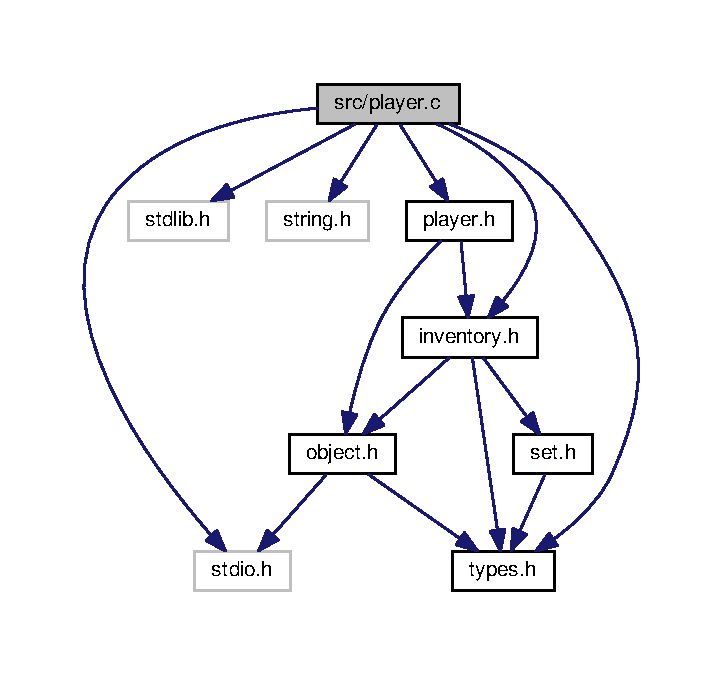
\includegraphics[width=347pt]{player_8c__incl}
\end{center}
\end{figure}
\subsection*{Data Structures}
\begin{DoxyCompactItemize}
\item 
struct \hyperlink{struct__Player}{\+\_\+\+Player}
\begin{DoxyCompactList}\small\item\em player definition \end{DoxyCompactList}\end{DoxyCompactItemize}
\subsection*{Functions}
\begin{DoxyCompactItemize}
\item 
\hyperlink{player_8h_af30e2030635a69690f85e48bc6ef202f}{Player} $\ast$ \hyperlink{player_8c_a97ea1d0deda3c51ef6ce63a13dab7a38}{player\+\_\+create} (\hyperlink{types_8h_a845e604fb28f7e3d97549da3448149d3}{Id} id)
\begin{DoxyCompactList}\small\item\em creates a player \end{DoxyCompactList}\item 
\hyperlink{types_8h_a32c27cc471df37f4fc818d65de0a56c4}{S\+T\+A\+T\+US} \hyperlink{player_8c_a4a602c75f8e3391cbd288c35a83a10fe}{player\+\_\+destroy} (\hyperlink{player_8h_af30e2030635a69690f85e48bc6ef202f}{Player} $\ast$p)
\begin{DoxyCompactList}\small\item\em frees memory \end{DoxyCompactList}\item 
char $\ast$ \hyperlink{player_8c_aaec42336dad00b854be6f071c653d645}{player\+\_\+get\+\_\+name} (\hyperlink{player_8h_af30e2030635a69690f85e48bc6ef202f}{Player} $\ast$p)
\begin{DoxyCompactList}\small\item\em gets the name of a player \end{DoxyCompactList}\item 
\hyperlink{types_8h_a845e604fb28f7e3d97549da3448149d3}{Id} \hyperlink{player_8c_ace9de3676a44420727bcc1d2935ae3e4}{player\+\_\+get\+\_\+id} (\hyperlink{player_8h_af30e2030635a69690f85e48bc6ef202f}{Player} $\ast$p)
\begin{DoxyCompactList}\small\item\em gets the id of a player \end{DoxyCompactList}\item 
\hyperlink{types_8h_a845e604fb28f7e3d97549da3448149d3}{Id} \hyperlink{player_8c_a00fd04dabfe1024ea62fe7c335097db7}{player\+\_\+get\+\_\+location} (\hyperlink{player_8h_af30e2030635a69690f85e48bc6ef202f}{Player} $\ast$p)
\begin{DoxyCompactList}\small\item\em gets the location of an player \end{DoxyCompactList}\item 
\hyperlink{types_8h_a845e604fb28f7e3d97549da3448149d3}{Id} \hyperlink{player_8c_afdb5019868014ca1647d716989664795}{player\+\_\+get\+\_\+object} (\hyperlink{player_8h_af30e2030635a69690f85e48bc6ef202f}{Player} $\ast$p, int position)
\begin{DoxyCompactList}\small\item\em gets an object \end{DoxyCompactList}\item 
\hyperlink{inventory_8h_a2253bf64ac4ce6a9c1d6f39c0b0d32a3}{Inventory} $\ast$ \hyperlink{player_8c_a727c2314037de6f622a513eb1291838f}{player\+\_\+get\+\_\+inventory} (\hyperlink{player_8h_af30e2030635a69690f85e48bc6ef202f}{Player} $\ast$p)
\begin{DoxyCompactList}\small\item\em gets an inventory \end{DoxyCompactList}\item 
\hyperlink{types_8h_a32c27cc471df37f4fc818d65de0a56c4}{S\+T\+A\+T\+US} \hyperlink{player_8c_a5c123d5c69f8d8fa0610c8212e56a3cd}{player\+\_\+set\+\_\+name} (\hyperlink{player_8h_af30e2030635a69690f85e48bc6ef202f}{Player} $\ast$p, char $\ast$name)
\begin{DoxyCompactList}\small\item\em sets name \end{DoxyCompactList}\item 
\hyperlink{types_8h_a32c27cc471df37f4fc818d65de0a56c4}{S\+T\+A\+T\+US} \hyperlink{player_8c_a1df02c30af1e7fd4ed798b62823d0206}{player\+\_\+set\+\_\+id} (\hyperlink{player_8h_af30e2030635a69690f85e48bc6ef202f}{Player} $\ast$p, \hyperlink{types_8h_a845e604fb28f7e3d97549da3448149d3}{Id} id)
\begin{DoxyCompactList}\small\item\em sets an id for a player \end{DoxyCompactList}\item 
\hyperlink{types_8h_a3e5b8192e7d9ffaf3542f1210aec18dd}{B\+O\+OL} \hyperlink{player_8c_a50d2d4bf00b796ffd28bd91bfcfd4685}{player\+\_\+has\+\_\+id} (\hyperlink{player_8h_af30e2030635a69690f85e48bc6ef202f}{Player} $\ast$p, \hyperlink{types_8h_a845e604fb28f7e3d97549da3448149d3}{Id} id)
\begin{DoxyCompactList}\small\item\em checks if player has an id \end{DoxyCompactList}\item 
\hyperlink{types_8h_a32c27cc471df37f4fc818d65de0a56c4}{S\+T\+A\+T\+US} \hyperlink{player_8c_a53cf87aa437ae42972050bd6da169888}{player\+\_\+set\+\_\+location} (\hyperlink{player_8h_af30e2030635a69690f85e48bc6ef202f}{Player} $\ast$p, \hyperlink{types_8h_a845e604fb28f7e3d97549da3448149d3}{Id} location)
\begin{DoxyCompactList}\small\item\em sets location \end{DoxyCompactList}\item 
\hyperlink{types_8h_a32c27cc471df37f4fc818d65de0a56c4}{S\+T\+A\+T\+US} \hyperlink{player_8c_a4096c89077192eedd36aebdba24e9e5e}{player\+\_\+set\+\_\+object} (\hyperlink{player_8h_af30e2030635a69690f85e48bc6ef202f}{Player} $\ast$p, \hyperlink{types_8h_a845e604fb28f7e3d97549da3448149d3}{Id} id)
\begin{DoxyCompactList}\small\item\em sets object \end{DoxyCompactList}\item 
\hyperlink{types_8h_a3e5b8192e7d9ffaf3542f1210aec18dd}{B\+O\+OL} \hyperlink{player_8c_a8b27bf719c2fe3fa9a4712d28dc6f316}{player\+\_\+inventory\+\_\+is\+\_\+empty} (\hyperlink{player_8h_af30e2030635a69690f85e48bc6ef202f}{Player} $\ast$p)
\begin{DoxyCompactList}\small\item\em checks if inventory is empty \end{DoxyCompactList}\item 
\hyperlink{types_8h_a3e5b8192e7d9ffaf3542f1210aec18dd}{B\+O\+OL} \hyperlink{player_8c_a5b4a99b2bcfc728a1bc61d7d33db649e}{player\+\_\+inventory\+\_\+is\+\_\+full} (\hyperlink{player_8h_af30e2030635a69690f85e48bc6ef202f}{Player} $\ast$p)
\begin{DoxyCompactList}\small\item\em checks if inventory is full \end{DoxyCompactList}\item 
\hyperlink{types_8h_a32c27cc471df37f4fc818d65de0a56c4}{S\+T\+A\+T\+US} \hyperlink{player_8c_a45c2b556f12fb90a1b9940bf8d79841f}{player\+\_\+remove\+\_\+object} (\hyperlink{player_8h_af30e2030635a69690f85e48bc6ef202f}{Player} $\ast$p, \hyperlink{types_8h_a845e604fb28f7e3d97549da3448149d3}{Id} id)
\begin{DoxyCompactList}\small\item\em removes an object \end{DoxyCompactList}\end{DoxyCompactItemize}


\subsection{Detailed Description}
Implements the game player commands. 

The player will be the one doing every action, such as picking an object or moving to a certain parts. It is in charge of getting the commands done.

\begin{DoxyAuthor}{Author}
Borja Pérez 
\end{DoxyAuthor}
\begin{DoxyVersion}{Version}
1.\+6 
\end{DoxyVersion}
\begin{DoxyDate}{Date}
09-\/04-\/2018 
\end{DoxyDate}


\subsection{Function Documentation}
\index{player.\+c@{player.\+c}!player\+\_\+create@{player\+\_\+create}}
\index{player\+\_\+create@{player\+\_\+create}!player.\+c@{player.\+c}}
\subsubsection[{\texorpdfstring{player\+\_\+create(\+Id id)}{player_create(Id id)}}]{\setlength{\rightskip}{0pt plus 5cm}{\bf Player}$\ast$ player\+\_\+create (
\begin{DoxyParamCaption}
\item[{{\bf Id}}]{id}
\end{DoxyParamCaption}
)}\hypertarget{player_8c_a97ea1d0deda3c51ef6ce63a13dab7a38}{}\label{player_8c_a97ea1d0deda3c51ef6ce63a13dab7a38}


creates a player 

It creates a new object initializing the variables of the structure.

\begin{DoxyAuthor}{Author}
Borja Pérez 
\end{DoxyAuthor}

\begin{DoxyParams}{Parameters}
{\em id} & long int. \\
\hline
\end{DoxyParams}
\begin{DoxyReturn}{Returns}
pointer to player, N\+U\+LL if something goes wrong. 
\end{DoxyReturn}
\index{player.\+c@{player.\+c}!player\+\_\+destroy@{player\+\_\+destroy}}
\index{player\+\_\+destroy@{player\+\_\+destroy}!player.\+c@{player.\+c}}
\subsubsection[{\texorpdfstring{player\+\_\+destroy(\+Player $\ast$p)}{player_destroy(Player *p)}}]{\setlength{\rightskip}{0pt plus 5cm}{\bf S\+T\+A\+T\+US} player\+\_\+destroy (
\begin{DoxyParamCaption}
\item[{{\bf Player} $\ast$}]{p}
\end{DoxyParamCaption}
)}\hypertarget{player_8c_a4a602c75f8e3391cbd288c35a83a10fe}{}\label{player_8c_a4a602c75f8e3391cbd288c35a83a10fe}


frees memory 

Receives pointer to player and frees the memory it occupied.

\begin{DoxyAuthor}{Author}
Borja Pérez 
\end{DoxyAuthor}

\begin{DoxyParams}{Parameters}
{\em p} & pointer to player. \\
\hline
\end{DoxyParams}
\begin{DoxyReturn}{Returns}
S\+T\+A\+T\+US, E\+R\+R\+OR if argument received is N\+U\+LL, if not, OK. 
\end{DoxyReturn}
\index{player.\+c@{player.\+c}!player\+\_\+get\+\_\+id@{player\+\_\+get\+\_\+id}}
\index{player\+\_\+get\+\_\+id@{player\+\_\+get\+\_\+id}!player.\+c@{player.\+c}}
\subsubsection[{\texorpdfstring{player\+\_\+get\+\_\+id(\+Player $\ast$p)}{player_get_id(Player *p)}}]{\setlength{\rightskip}{0pt plus 5cm}{\bf Id} player\+\_\+get\+\_\+id (
\begin{DoxyParamCaption}
\item[{{\bf Player} $\ast$}]{p}
\end{DoxyParamCaption}
)}\hypertarget{player_8c_ace9de3676a44420727bcc1d2935ae3e4}{}\label{player_8c_ace9de3676a44420727bcc1d2935ae3e4}


gets the id of a player 

Function in charge of getting the id of an player by using a pointer to it.

\begin{DoxyAuthor}{Author}
Borja Pérez 
\end{DoxyAuthor}

\begin{DoxyParams}{Parameters}
{\em p} & pointer to player. \\
\hline
\end{DoxyParams}
\begin{DoxyReturn}{Returns}
Id, N\+O\+\_\+\+ID if object is pointing N\+U\+LL. 
\end{DoxyReturn}
\index{player.\+c@{player.\+c}!player\+\_\+get\+\_\+inventory@{player\+\_\+get\+\_\+inventory}}
\index{player\+\_\+get\+\_\+inventory@{player\+\_\+get\+\_\+inventory}!player.\+c@{player.\+c}}
\subsubsection[{\texorpdfstring{player\+\_\+get\+\_\+inventory(\+Player $\ast$p)}{player_get_inventory(Player *p)}}]{\setlength{\rightskip}{0pt plus 5cm}{\bf Inventory}$\ast$ player\+\_\+get\+\_\+inventory (
\begin{DoxyParamCaption}
\item[{{\bf Player} $\ast$}]{p}
\end{DoxyParamCaption}
)}\hypertarget{player_8c_a727c2314037de6f622a513eb1291838f}{}\label{player_8c_a727c2314037de6f622a513eb1291838f}


gets an inventory 

The player has an inventory that enables the player to take more than one object.

\begin{DoxyAuthor}{Author}
Borja Pérez 
\end{DoxyAuthor}

\begin{DoxyParams}{Parameters}
{\em p} & pointer to player. \\
\hline
\end{DoxyParams}
\begin{DoxyReturn}{Returns}
pointer to inventory (objects). 
\end{DoxyReturn}
\index{player.\+c@{player.\+c}!player\+\_\+get\+\_\+location@{player\+\_\+get\+\_\+location}}
\index{player\+\_\+get\+\_\+location@{player\+\_\+get\+\_\+location}!player.\+c@{player.\+c}}
\subsubsection[{\texorpdfstring{player\+\_\+get\+\_\+location(\+Player $\ast$p)}{player_get_location(Player *p)}}]{\setlength{\rightskip}{0pt plus 5cm}{\bf Id} player\+\_\+get\+\_\+location (
\begin{DoxyParamCaption}
\item[{{\bf Player} $\ast$}]{p}
\end{DoxyParamCaption}
)}\hypertarget{player_8c_a00fd04dabfe1024ea62fe7c335097db7}{}\label{player_8c_a00fd04dabfe1024ea62fe7c335097db7}


gets the location of an player 

Function in charge of getting the location of a player and returning it.

\begin{DoxyAuthor}{Author}
Borja Pérez 
\end{DoxyAuthor}

\begin{DoxyParams}{Parameters}
{\em p} & pointer to player \\
\hline
\end{DoxyParams}
\begin{DoxyReturn}{Returns}
Id, N\+O\+\_\+\+ID if inventory is pointing N\+U\+LL. 
\end{DoxyReturn}
\index{player.\+c@{player.\+c}!player\+\_\+get\+\_\+name@{player\+\_\+get\+\_\+name}}
\index{player\+\_\+get\+\_\+name@{player\+\_\+get\+\_\+name}!player.\+c@{player.\+c}}
\subsubsection[{\texorpdfstring{player\+\_\+get\+\_\+name(\+Player $\ast$p)}{player_get_name(Player *p)}}]{\setlength{\rightskip}{0pt plus 5cm}char$\ast$ player\+\_\+get\+\_\+name (
\begin{DoxyParamCaption}
\item[{{\bf Player} $\ast$}]{p}
\end{DoxyParamCaption}
)}\hypertarget{player_8c_aaec42336dad00b854be6f071c653d645}{}\label{player_8c_aaec42336dad00b854be6f071c653d645}


gets the name of a player 

Function in charge of showing the name of a player that has already been set.

\begin{DoxyAuthor}{Author}
Borja Pérez 
\end{DoxyAuthor}

\begin{DoxyParams}{Parameters}
{\em p} & pointer to object. \\
\hline
\end{DoxyParams}
\begin{DoxyReturn}{Returns}
char (name of the player). 
\end{DoxyReturn}
\index{player.\+c@{player.\+c}!player\+\_\+get\+\_\+object@{player\+\_\+get\+\_\+object}}
\index{player\+\_\+get\+\_\+object@{player\+\_\+get\+\_\+object}!player.\+c@{player.\+c}}
\subsubsection[{\texorpdfstring{player\+\_\+get\+\_\+object(\+Player $\ast$p, int position)}{player_get_object(Player *p, int position)}}]{\setlength{\rightskip}{0pt plus 5cm}{\bf Id} player\+\_\+get\+\_\+object (
\begin{DoxyParamCaption}
\item[{{\bf Player} $\ast$}]{p, }
\item[{int}]{position}
\end{DoxyParamCaption}
)}\hypertarget{player_8c_afdb5019868014ca1647d716989664795}{}\label{player_8c_afdb5019868014ca1647d716989664795}


gets an object 

Function in charge of getting the object that the player will carry.

\begin{DoxyAuthor}{Author}
Borja Pérez 
\end{DoxyAuthor}

\begin{DoxyParams}{Parameters}
{\em p} & pointer to player. \\
\hline
{\em position} & int (position of the object). \\
\hline
\end{DoxyParams}
\begin{DoxyReturn}{Returns}
Id, N\+O\+\_\+\+ID if inventory is pointing N\+U\+LL. 
\end{DoxyReturn}
\index{player.\+c@{player.\+c}!player\+\_\+has\+\_\+id@{player\+\_\+has\+\_\+id}}
\index{player\+\_\+has\+\_\+id@{player\+\_\+has\+\_\+id}!player.\+c@{player.\+c}}
\subsubsection[{\texorpdfstring{player\+\_\+has\+\_\+id(\+Player $\ast$p, Id id)}{player_has_id(Player *p, Id id)}}]{\setlength{\rightskip}{0pt plus 5cm}{\bf B\+O\+OL} player\+\_\+has\+\_\+id (
\begin{DoxyParamCaption}
\item[{{\bf Player} $\ast$}]{p, }
\item[{{\bf Id}}]{id}
\end{DoxyParamCaption}
)}\hypertarget{player_8c_a50d2d4bf00b796ffd28bd91bfcfd4685}{}\label{player_8c_a50d2d4bf00b796ffd28bd91bfcfd4685}


checks if player has an id 

Function in charge of making sure that the player is getting an id.

\begin{DoxyAuthor}{Author}
Borja Pérez 
\end{DoxyAuthor}

\begin{DoxyParams}{Parameters}
{\em p} & pointer to player. \\
\hline
{\em id} & long int. \\
\hline
\end{DoxyParams}
\begin{DoxyReturn}{Returns}
B\+O\+OL, F\+A\+L\+SE if when checking is not correct, if it is correct, T\+R\+UE. 
\end{DoxyReturn}
\index{player.\+c@{player.\+c}!player\+\_\+inventory\+\_\+is\+\_\+empty@{player\+\_\+inventory\+\_\+is\+\_\+empty}}
\index{player\+\_\+inventory\+\_\+is\+\_\+empty@{player\+\_\+inventory\+\_\+is\+\_\+empty}!player.\+c@{player.\+c}}
\subsubsection[{\texorpdfstring{player\+\_\+inventory\+\_\+is\+\_\+empty(\+Player $\ast$p)}{player_inventory_is_empty(Player *p)}}]{\setlength{\rightskip}{0pt plus 5cm}{\bf B\+O\+OL} player\+\_\+inventory\+\_\+is\+\_\+empty (
\begin{DoxyParamCaption}
\item[{{\bf Player} $\ast$}]{p}
\end{DoxyParamCaption}
)}\hypertarget{player_8c_a8b27bf719c2fe3fa9a4712d28dc6f316}{}\label{player_8c_a8b27bf719c2fe3fa9a4712d28dc6f316}


checks if inventory is empty 

Function in charge of making sure that the inventory is empty using a pointer to player in order to work with other modules more easily.

\begin{DoxyAuthor}{Author}
Borja Pérez 
\end{DoxyAuthor}

\begin{DoxyParams}{Parameters}
{\em p} & pointer to player. \\
\hline
\end{DoxyParams}
\begin{DoxyReturn}{Returns}
B\+O\+OL, F\+A\+L\+SE if when checking is not correct, if it is correct, T\+R\+UE. 
\end{DoxyReturn}
\index{player.\+c@{player.\+c}!player\+\_\+inventory\+\_\+is\+\_\+full@{player\+\_\+inventory\+\_\+is\+\_\+full}}
\index{player\+\_\+inventory\+\_\+is\+\_\+full@{player\+\_\+inventory\+\_\+is\+\_\+full}!player.\+c@{player.\+c}}
\subsubsection[{\texorpdfstring{player\+\_\+inventory\+\_\+is\+\_\+full(\+Player $\ast$p)}{player_inventory_is_full(Player *p)}}]{\setlength{\rightskip}{0pt plus 5cm}{\bf B\+O\+OL} player\+\_\+inventory\+\_\+is\+\_\+full (
\begin{DoxyParamCaption}
\item[{{\bf Player} $\ast$}]{p}
\end{DoxyParamCaption}
)}\hypertarget{player_8c_a5b4a99b2bcfc728a1bc61d7d33db649e}{}\label{player_8c_a5b4a99b2bcfc728a1bc61d7d33db649e}


checks if inventory is full 

Function in charge of making sure that the inventory is full using a pointer to player in order to work with other modules more easily.

\begin{DoxyAuthor}{Author}
Borja Pérez 
\end{DoxyAuthor}

\begin{DoxyParams}{Parameters}
{\em p} & pointer to player. \\
\hline
\end{DoxyParams}
\begin{DoxyReturn}{Returns}
B\+O\+OL, F\+A\+L\+SE if when checking is not correct, if it is correct, T\+R\+UE. 
\end{DoxyReturn}
\index{player.\+c@{player.\+c}!player\+\_\+remove\+\_\+object@{player\+\_\+remove\+\_\+object}}
\index{player\+\_\+remove\+\_\+object@{player\+\_\+remove\+\_\+object}!player.\+c@{player.\+c}}
\subsubsection[{\texorpdfstring{player\+\_\+remove\+\_\+object(\+Player $\ast$p, Id id)}{player_remove_object(Player *p, Id id)}}]{\setlength{\rightskip}{0pt plus 5cm}{\bf S\+T\+A\+T\+US} player\+\_\+remove\+\_\+object (
\begin{DoxyParamCaption}
\item[{{\bf Player} $\ast$}]{p, }
\item[{{\bf Id}}]{id}
\end{DoxyParamCaption}
)}\hypertarget{player_8c_a45c2b556f12fb90a1b9940bf8d79841f}{}\label{player_8c_a45c2b556f12fb90a1b9940bf8d79841f}


removes an object 

Deletes an object by using other functions prepared for this specific one.

\begin{DoxyAuthor}{Author}
Borja Pérez 
\end{DoxyAuthor}

\begin{DoxyParams}{Parameters}
{\em p} & pointer to player. \\
\hline
{\em id} & long int. \\
\hline
\end{DoxyParams}
\begin{DoxyReturn}{Returns}
S\+T\+A\+T\+US, E\+R\+R\+OR if argument received is N\+U\+LL, if not, OK. 
\end{DoxyReturn}
\index{player.\+c@{player.\+c}!player\+\_\+set\+\_\+id@{player\+\_\+set\+\_\+id}}
\index{player\+\_\+set\+\_\+id@{player\+\_\+set\+\_\+id}!player.\+c@{player.\+c}}
\subsubsection[{\texorpdfstring{player\+\_\+set\+\_\+id(\+Player $\ast$p, Id id)}{player_set_id(Player *p, Id id)}}]{\setlength{\rightskip}{0pt plus 5cm}{\bf S\+T\+A\+T\+US} player\+\_\+set\+\_\+id (
\begin{DoxyParamCaption}
\item[{{\bf Player} $\ast$}]{p, }
\item[{{\bf Id}}]{id}
\end{DoxyParamCaption}
)}\hypertarget{player_8c_a1df02c30af1e7fd4ed798b62823d0206}{}\label{player_8c_a1df02c30af1e7fd4ed798b62823d0206}


sets an id for a player 

Function in charge of changing a player\textquotesingle{}s id.

\begin{DoxyAuthor}{Author}
Borja Pérez 
\end{DoxyAuthor}

\begin{DoxyParams}{Parameters}
{\em p} & pointer to player. \\
\hline
{\em id} & long int. \\
\hline
\end{DoxyParams}
\begin{DoxyReturn}{Returns}
S\+T\+A\+T\+US, E\+R\+R\+OR if argument received is N\+U\+LL, if not, OK. 
\end{DoxyReturn}
\index{player.\+c@{player.\+c}!player\+\_\+set\+\_\+location@{player\+\_\+set\+\_\+location}}
\index{player\+\_\+set\+\_\+location@{player\+\_\+set\+\_\+location}!player.\+c@{player.\+c}}
\subsubsection[{\texorpdfstring{player\+\_\+set\+\_\+location(\+Player $\ast$p, Id location)}{player_set_location(Player *p, Id location)}}]{\setlength{\rightskip}{0pt plus 5cm}{\bf S\+T\+A\+T\+US} player\+\_\+set\+\_\+location (
\begin{DoxyParamCaption}
\item[{{\bf Player} $\ast$}]{p, }
\item[{{\bf Id}}]{location}
\end{DoxyParamCaption}
)}\hypertarget{player_8c_a53cf87aa437ae42972050bd6da169888}{}\label{player_8c_a53cf87aa437ae42972050bd6da169888}


sets location 

Changes a player\textquotesingle{}s location.

\begin{DoxyAuthor}{Author}
Borja Pérez 
\end{DoxyAuthor}

\begin{DoxyParams}{Parameters}
{\em p} & pointer to player. \\
\hline
{\em location} & The id of the player\textquotesingle{}s location. \\
\hline
\end{DoxyParams}
\begin{DoxyReturn}{Returns}
S\+T\+A\+T\+US, E\+R\+R\+OR if argument received is N\+U\+LL, if not, OK. 
\end{DoxyReturn}
\index{player.\+c@{player.\+c}!player\+\_\+set\+\_\+name@{player\+\_\+set\+\_\+name}}
\index{player\+\_\+set\+\_\+name@{player\+\_\+set\+\_\+name}!player.\+c@{player.\+c}}
\subsubsection[{\texorpdfstring{player\+\_\+set\+\_\+name(\+Player $\ast$p, char $\ast$name)}{player_set_name(Player *p, char *name)}}]{\setlength{\rightskip}{0pt plus 5cm}{\bf S\+T\+A\+T\+US} player\+\_\+set\+\_\+name (
\begin{DoxyParamCaption}
\item[{{\bf Player} $\ast$}]{p, }
\item[{char $\ast$}]{name}
\end{DoxyParamCaption}
)}\hypertarget{player_8c_a5c123d5c69f8d8fa0610c8212e56a3cd}{}\label{player_8c_a5c123d5c69f8d8fa0610c8212e56a3cd}


sets name 

Function in charge of changing the name of a player.

\begin{DoxyAuthor}{Author}
Borja Pérez 
\end{DoxyAuthor}

\begin{DoxyParams}{Parameters}
{\em p} & pointer to player. \\
\hline
{\em name} & char( string for the name of the player). \\
\hline
\end{DoxyParams}
\begin{DoxyReturn}{Returns}
S\+T\+A\+T\+US, E\+R\+R\+OR if argument received is N\+U\+LL, if not, OK. 
\end{DoxyReturn}
\index{player.\+c@{player.\+c}!player\+\_\+set\+\_\+object@{player\+\_\+set\+\_\+object}}
\index{player\+\_\+set\+\_\+object@{player\+\_\+set\+\_\+object}!player.\+c@{player.\+c}}
\subsubsection[{\texorpdfstring{player\+\_\+set\+\_\+object(\+Player $\ast$p, Id id)}{player_set_object(Player *p, Id id)}}]{\setlength{\rightskip}{0pt plus 5cm}{\bf S\+T\+A\+T\+US} player\+\_\+set\+\_\+object (
\begin{DoxyParamCaption}
\item[{{\bf Player} $\ast$}]{p, }
\item[{{\bf Id}}]{id}
\end{DoxyParamCaption}
)}\hypertarget{player_8c_a4096c89077192eedd36aebdba24e9e5e}{}\label{player_8c_a4096c89077192eedd36aebdba24e9e5e}


sets object 

Changes the object carried by a player.

\begin{DoxyAuthor}{Author}
Borja Pérez 
\end{DoxyAuthor}

\begin{DoxyParams}{Parameters}
{\em p} & pointer to player. \\
\hline
{\em id} & long int. \\
\hline
\end{DoxyParams}
\begin{DoxyReturn}{Returns}
S\+T\+A\+T\+US, E\+R\+R\+OR if argument received is N\+U\+LL, if not, OK. 
\end{DoxyReturn}

\hypertarget{player__test_8c}{}\section{src/player\+\_\+test.c File Reference}
\label{player__test_8c}\index{src/player\+\_\+test.\+c@{src/player\+\_\+test.\+c}}


It tests player module.  


{\ttfamily \#include $<$stdio.\+h$>$}\\*
{\ttfamily \#include $<$stdlib.\+h$>$}\\*
{\ttfamily \#include $<$string.\+h$>$}\\*
{\ttfamily \#include \char`\"{}player.\+h\char`\"{}}\\*
{\ttfamily \#include \char`\"{}player\+\_\+test.\+h\char`\"{}}\\*
{\ttfamily \#include \char`\"{}test.\+h\char`\"{}}\\*
{\ttfamily \#include \char`\"{}inventory.\+h\char`\"{}}\\*
Include dependency graph for player\+\_\+test.\+c\+:
\nopagebreak
\begin{figure}[H]
\begin{center}
\leavevmode
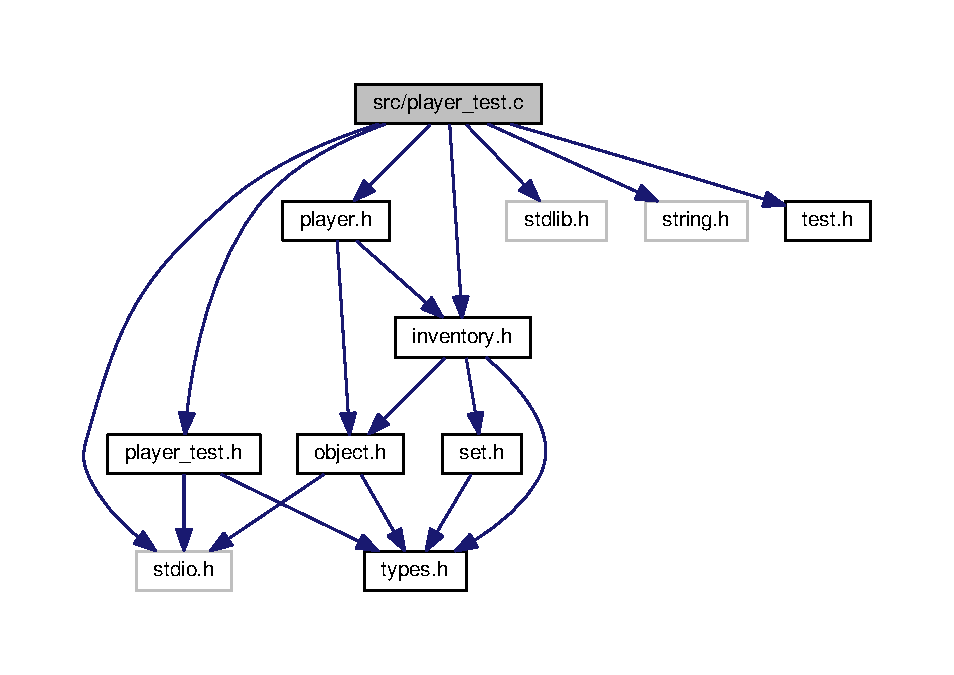
\includegraphics[width=350pt]{player__test_8c__incl}
\end{center}
\end{figure}
\subsection*{Macros}
\begin{DoxyCompactItemize}
\item 
\#define \hyperlink{player__test_8c_a2a77d2f2c5b698c69c19e1f8782bf709}{M\+A\+X\+\_\+\+T\+E\+S\+TS}~16
\end{DoxyCompactItemize}
\subsection*{Functions}
\begin{DoxyCompactItemize}
\item 
int \hyperlink{player__test_8c_a3c04138a5bfe5d72780bb7e82a18e627}{main} (int argc, char $\ast$$\ast$argv)
\begin{DoxyCompactList}\small\item\em Main function for player unit tests. \end{DoxyCompactList}\item 
void \hyperlink{player__test_8c_ab29768452373e16bb6aaa1f7998f62fb}{test1\+\_\+player\+\_\+create} ()
\item 
void \hyperlink{player__test_8c_a4f6eca5f9d8c08d2a7fc70c209ecf854}{test2\+\_\+player\+\_\+create} ()
\item 
void \hyperlink{player__test_8c_aae84b37f9cc0fbde18a62807385c359a}{test3\+\_\+player\+\_\+create} ()
\item 
void \hyperlink{player__test_8c_a14d75d99f9fce3bd703b0c242c8690f9}{test1\+\_\+player\+\_\+destroy} ()
\item 
void \hyperlink{player__test_8c_ae873be01647faf96d3906aa9629e87f0}{test2\+\_\+player\+\_\+destroy} ()
\item 
void \hyperlink{player__test_8c_a53eb6ee101f01fe988c5da03129d2e2f}{test1\+\_\+player\+\_\+get\+\_\+object} ()
\item 
void \hyperlink{player__test_8c_a83e8fea42cd87151cd67d0643a78134f}{test2\+\_\+player\+\_\+get\+\_\+object} ()
\item 
void \hyperlink{player__test_8c_ac8d8b030a98c0e44f4e98e08cda59537}{test1\+\_\+player\+\_\+set\+\_\+object} ()
\item 
void \hyperlink{player__test_8c_a9e7db6b857907187146df64abd16aca5}{test2\+\_\+player\+\_\+set\+\_\+object} ()
\item 
void \hyperlink{player__test_8c_a0685839b423f685dcdabb7b9fe411cd1}{test1\+\_\+player\+\_\+remove\+\_\+object} ()
\item 
void \hyperlink{player__test_8c_af9e74e12ad6961761f1ff61afa56be3e}{test2\+\_\+player\+\_\+remove\+\_\+object} ()
\item 
void \hyperlink{player__test_8c_a8841b3b289649eb76edaa8110ad5899c}{test1\+\_\+player\+\_\+has\+\_\+id} ()
\item 
void \hyperlink{player__test_8c_afa75f333281fc35b24968a5629f09b0b}{test2\+\_\+player\+\_\+has\+\_\+id} ()
\item 
void \hyperlink{player__test_8c_a3b450c7540eddb05810dc9c25e4de082}{test3\+\_\+player\+\_\+has\+\_\+id} ()
\item 
void \hyperlink{player__test_8c_ad4a86b57bc18593265c205d7b27b9ecb}{test1\+\_\+player\+\_\+get\+\_\+inventory} ()
\item 
void \hyperlink{player__test_8c_a8f3a62c708fbed848568841ca8b1cd26}{test2\+\_\+player\+\_\+get\+\_\+inventory} ()
\end{DoxyCompactItemize}


\subsection{Detailed Description}
It tests player module. 

\begin{DoxyAuthor}{Author}
Andres Mena 
\end{DoxyAuthor}
\begin{DoxyVersion}{Version}
1.\+0 
\end{DoxyVersion}
\begin{DoxyDate}{Date}
31-\/03-\/2018 
\end{DoxyDate}
\begin{DoxyCopyright}{Copyright}
G\+NU Public License 
\end{DoxyCopyright}


\subsection{Macro Definition Documentation}
\index{player\+\_\+test.\+c@{player\+\_\+test.\+c}!M\+A\+X\+\_\+\+T\+E\+S\+TS@{M\+A\+X\+\_\+\+T\+E\+S\+TS}}
\index{M\+A\+X\+\_\+\+T\+E\+S\+TS@{M\+A\+X\+\_\+\+T\+E\+S\+TS}!player\+\_\+test.\+c@{player\+\_\+test.\+c}}
\subsubsection[{\texorpdfstring{M\+A\+X\+\_\+\+T\+E\+S\+TS}{MAX_TESTS}}]{\setlength{\rightskip}{0pt plus 5cm}\#define M\+A\+X\+\_\+\+T\+E\+S\+TS~16}\hypertarget{player__test_8c_a2a77d2f2c5b698c69c19e1f8782bf709}{}\label{player__test_8c_a2a77d2f2c5b698c69c19e1f8782bf709}
Max amount of tests posible 

\subsection{Function Documentation}
\index{player\+\_\+test.\+c@{player\+\_\+test.\+c}!main@{main}}
\index{main@{main}!player\+\_\+test.\+c@{player\+\_\+test.\+c}}
\subsubsection[{\texorpdfstring{main(int argc, char $\ast$$\ast$argv)}{main(int argc, char **argv)}}]{\setlength{\rightskip}{0pt plus 5cm}int main (
\begin{DoxyParamCaption}
\item[{int}]{argc, }
\item[{char $\ast$$\ast$}]{argv}
\end{DoxyParamCaption}
)}\hypertarget{player__test_8c_a3c04138a5bfe5d72780bb7e82a18e627}{}\label{player__test_8c_a3c04138a5bfe5d72780bb7e82a18e627}


Main function for player unit tests. 

You may execute A\+LL or a S\+I\+N\+G\+LE test 1.-\/ No parameter -\/$>$ A\+LL test are executed 2.-\/ A number means a particular test (the one identified by that number) is executed \index{player\+\_\+test.\+c@{player\+\_\+test.\+c}!test1\+\_\+player\+\_\+create@{test1\+\_\+player\+\_\+create}}
\index{test1\+\_\+player\+\_\+create@{test1\+\_\+player\+\_\+create}!player\+\_\+test.\+c@{player\+\_\+test.\+c}}
\subsubsection[{\texorpdfstring{test1\+\_\+player\+\_\+create()}{test1_player_create()}}]{\setlength{\rightskip}{0pt plus 5cm}void test1\+\_\+player\+\_\+create (
\begin{DoxyParamCaption}
{}
\end{DoxyParamCaption}
)}\hypertarget{player__test_8c_ab29768452373e16bb6aaa1f7998f62fb}{}\label{player__test_8c_ab29768452373e16bb6aaa1f7998f62fb}
\begin{DoxyRefDesc}{Test}
\item[\hyperlink{test__test000105}{Test}]Test player creation \end{DoxyRefDesc}
\begin{DoxyPrecond}{Precondition}
ID 
\end{DoxyPrecond}
\begin{DoxyPostcond}{Postcondition}
Non N\+U\+LL pointer to player 
\end{DoxyPostcond}
\index{player\+\_\+test.\+c@{player\+\_\+test.\+c}!test1\+\_\+player\+\_\+destroy@{test1\+\_\+player\+\_\+destroy}}
\index{test1\+\_\+player\+\_\+destroy@{test1\+\_\+player\+\_\+destroy}!player\+\_\+test.\+c@{player\+\_\+test.\+c}}
\subsubsection[{\texorpdfstring{test1\+\_\+player\+\_\+destroy()}{test1_player_destroy()}}]{\setlength{\rightskip}{0pt plus 5cm}void test1\+\_\+player\+\_\+destroy (
\begin{DoxyParamCaption}
{}
\end{DoxyParamCaption}
)}\hypertarget{player__test_8c_a14d75d99f9fce3bd703b0c242c8690f9}{}\label{player__test_8c_a14d75d99f9fce3bd703b0c242c8690f9}
\begin{DoxyRefDesc}{Test}
\item[\hyperlink{test__test000108}{Test}]Test player creation \end{DoxyRefDesc}
\begin{DoxyPrecond}{Precondition}
N\+U\+LL pointer to player 
\end{DoxyPrecond}
\begin{DoxyPostcond}{Postcondition}
S\+T\+A\+T\+US == E\+R\+R\+OR 
\end{DoxyPostcond}
\index{player\+\_\+test.\+c@{player\+\_\+test.\+c}!test1\+\_\+player\+\_\+get\+\_\+inventory@{test1\+\_\+player\+\_\+get\+\_\+inventory}}
\index{test1\+\_\+player\+\_\+get\+\_\+inventory@{test1\+\_\+player\+\_\+get\+\_\+inventory}!player\+\_\+test.\+c@{player\+\_\+test.\+c}}
\subsubsection[{\texorpdfstring{test1\+\_\+player\+\_\+get\+\_\+inventory()}{test1_player_get_inventory()}}]{\setlength{\rightskip}{0pt plus 5cm}void test1\+\_\+player\+\_\+get\+\_\+inventory (
\begin{DoxyParamCaption}
{}
\end{DoxyParamCaption}
)}\hypertarget{player__test_8c_ad4a86b57bc18593265c205d7b27b9ecb}{}\label{player__test_8c_ad4a86b57bc18593265c205d7b27b9ecb}
\begin{DoxyRefDesc}{Test}
\item[\hyperlink{test__test000113}{Test}]Test player inventory \end{DoxyRefDesc}
\begin{DoxyPrecond}{Precondition}
N\+U\+LL pointer to player 
\end{DoxyPrecond}
\begin{DoxyPostcond}{Postcondition}
N\+U\+LL 
\end{DoxyPostcond}
\index{player\+\_\+test.\+c@{player\+\_\+test.\+c}!test1\+\_\+player\+\_\+get\+\_\+object@{test1\+\_\+player\+\_\+get\+\_\+object}}
\index{test1\+\_\+player\+\_\+get\+\_\+object@{test1\+\_\+player\+\_\+get\+\_\+object}!player\+\_\+test.\+c@{player\+\_\+test.\+c}}
\subsubsection[{\texorpdfstring{test1\+\_\+player\+\_\+get\+\_\+object()}{test1_player_get_object()}}]{\setlength{\rightskip}{0pt plus 5cm}void test1\+\_\+player\+\_\+get\+\_\+object (
\begin{DoxyParamCaption}
{}
\end{DoxyParamCaption}
)}\hypertarget{player__test_8c_a53eb6ee101f01fe988c5da03129d2e2f}{}\label{player__test_8c_a53eb6ee101f01fe988c5da03129d2e2f}
\begin{DoxyRefDesc}{Test}
\item[\hyperlink{test__test000115}{Test}]Test getting objects from player \end{DoxyRefDesc}
\begin{DoxyPrecond}{Precondition}
N\+U\+LL pointer to player 
\end{DoxyPrecond}
\begin{DoxyPostcond}{Postcondition}
N\+O\+\_\+\+ID 
\end{DoxyPostcond}
\index{player\+\_\+test.\+c@{player\+\_\+test.\+c}!test1\+\_\+player\+\_\+has\+\_\+id@{test1\+\_\+player\+\_\+has\+\_\+id}}
\index{test1\+\_\+player\+\_\+has\+\_\+id@{test1\+\_\+player\+\_\+has\+\_\+id}!player\+\_\+test.\+c@{player\+\_\+test.\+c}}
\subsubsection[{\texorpdfstring{test1\+\_\+player\+\_\+has\+\_\+id()}{test1_player_has_id()}}]{\setlength{\rightskip}{0pt plus 5cm}void test1\+\_\+player\+\_\+has\+\_\+id (
\begin{DoxyParamCaption}
{}
\end{DoxyParamCaption}
)}\hypertarget{player__test_8c_a8841b3b289649eb76edaa8110ad5899c}{}\label{player__test_8c_a8841b3b289649eb76edaa8110ad5899c}
\begin{DoxyRefDesc}{Test}
\item[\hyperlink{test__test000110}{Test}]Test if player has id \end{DoxyRefDesc}
\begin{DoxyPrecond}{Precondition}
N\+U\+LL pointer to player 
\end{DoxyPrecond}
\begin{DoxyPostcond}{Postcondition}
B\+O\+OL == F\+A\+L\+SE 
\end{DoxyPostcond}
\index{player\+\_\+test.\+c@{player\+\_\+test.\+c}!test1\+\_\+player\+\_\+remove\+\_\+object@{test1\+\_\+player\+\_\+remove\+\_\+object}}
\index{test1\+\_\+player\+\_\+remove\+\_\+object@{test1\+\_\+player\+\_\+remove\+\_\+object}!player\+\_\+test.\+c@{player\+\_\+test.\+c}}
\subsubsection[{\texorpdfstring{test1\+\_\+player\+\_\+remove\+\_\+object()}{test1_player_remove_object()}}]{\setlength{\rightskip}{0pt plus 5cm}void test1\+\_\+player\+\_\+remove\+\_\+object (
\begin{DoxyParamCaption}
{}
\end{DoxyParamCaption}
)}\hypertarget{player__test_8c_a0685839b423f685dcdabb7b9fe411cd1}{}\label{player__test_8c_a0685839b423f685dcdabb7b9fe411cd1}
\begin{DoxyRefDesc}{Test}
\item[\hyperlink{test__test000119}{Test}]Test removing objects from player \end{DoxyRefDesc}
\begin{DoxyPrecond}{Precondition}
N\+U\+LL pointer to player 
\end{DoxyPrecond}
\begin{DoxyPostcond}{Postcondition}
E\+R\+R\+OR 
\end{DoxyPostcond}
\index{player\+\_\+test.\+c@{player\+\_\+test.\+c}!test1\+\_\+player\+\_\+set\+\_\+object@{test1\+\_\+player\+\_\+set\+\_\+object}}
\index{test1\+\_\+player\+\_\+set\+\_\+object@{test1\+\_\+player\+\_\+set\+\_\+object}!player\+\_\+test.\+c@{player\+\_\+test.\+c}}
\subsubsection[{\texorpdfstring{test1\+\_\+player\+\_\+set\+\_\+object()}{test1_player_set_object()}}]{\setlength{\rightskip}{0pt plus 5cm}void test1\+\_\+player\+\_\+set\+\_\+object (
\begin{DoxyParamCaption}
{}
\end{DoxyParamCaption}
)}\hypertarget{player__test_8c_ac8d8b030a98c0e44f4e98e08cda59537}{}\label{player__test_8c_ac8d8b030a98c0e44f4e98e08cda59537}
\begin{DoxyRefDesc}{Test}
\item[\hyperlink{test__test000117}{Test}]Test setting objects to player \end{DoxyRefDesc}
\begin{DoxyPrecond}{Precondition}
N\+U\+LL pointer to player 
\end{DoxyPrecond}
\begin{DoxyPostcond}{Postcondition}
E\+R\+R\+OR 
\end{DoxyPostcond}
\index{player\+\_\+test.\+c@{player\+\_\+test.\+c}!test2\+\_\+player\+\_\+create@{test2\+\_\+player\+\_\+create}}
\index{test2\+\_\+player\+\_\+create@{test2\+\_\+player\+\_\+create}!player\+\_\+test.\+c@{player\+\_\+test.\+c}}
\subsubsection[{\texorpdfstring{test2\+\_\+player\+\_\+create()}{test2_player_create()}}]{\setlength{\rightskip}{0pt plus 5cm}void test2\+\_\+player\+\_\+create (
\begin{DoxyParamCaption}
{}
\end{DoxyParamCaption}
)}\hypertarget{player__test_8c_a4f6eca5f9d8c08d2a7fc70c209ecf854}{}\label{player__test_8c_a4f6eca5f9d8c08d2a7fc70c209ecf854}
\begin{DoxyRefDesc}{Test}
\item[\hyperlink{test__test000106}{Test}]Test player creation \end{DoxyRefDesc}
\begin{DoxyPrecond}{Precondition}
Player ID 
\end{DoxyPrecond}
\begin{DoxyPostcond}{Postcondition}
Player\+\_\+\+ID == Supplied player Id 
\end{DoxyPostcond}
\index{player\+\_\+test.\+c@{player\+\_\+test.\+c}!test2\+\_\+player\+\_\+destroy@{test2\+\_\+player\+\_\+destroy}}
\index{test2\+\_\+player\+\_\+destroy@{test2\+\_\+player\+\_\+destroy}!player\+\_\+test.\+c@{player\+\_\+test.\+c}}
\subsubsection[{\texorpdfstring{test2\+\_\+player\+\_\+destroy()}{test2_player_destroy()}}]{\setlength{\rightskip}{0pt plus 5cm}void test2\+\_\+player\+\_\+destroy (
\begin{DoxyParamCaption}
{}
\end{DoxyParamCaption}
)}\hypertarget{player__test_8c_ae873be01647faf96d3906aa9629e87f0}{}\label{player__test_8c_ae873be01647faf96d3906aa9629e87f0}
\begin{DoxyRefDesc}{Test}
\item[\hyperlink{test__test000109}{Test}]Test player creation \end{DoxyRefDesc}
\begin{DoxyPrecond}{Precondition}
Pointer to player 
\end{DoxyPrecond}
\begin{DoxyPostcond}{Postcondition}
S\+T\+A\+T\+US == OK 
\end{DoxyPostcond}
\index{player\+\_\+test.\+c@{player\+\_\+test.\+c}!test2\+\_\+player\+\_\+get\+\_\+inventory@{test2\+\_\+player\+\_\+get\+\_\+inventory}}
\index{test2\+\_\+player\+\_\+get\+\_\+inventory@{test2\+\_\+player\+\_\+get\+\_\+inventory}!player\+\_\+test.\+c@{player\+\_\+test.\+c}}
\subsubsection[{\texorpdfstring{test2\+\_\+player\+\_\+get\+\_\+inventory()}{test2_player_get_inventory()}}]{\setlength{\rightskip}{0pt plus 5cm}void test2\+\_\+player\+\_\+get\+\_\+inventory (
\begin{DoxyParamCaption}
{}
\end{DoxyParamCaption}
)}\hypertarget{player__test_8c_a8f3a62c708fbed848568841ca8b1cd26}{}\label{player__test_8c_a8f3a62c708fbed848568841ca8b1cd26}
\begin{DoxyRefDesc}{Test}
\item[\hyperlink{test__test000114}{Test}]Test player inventory \end{DoxyRefDesc}
\begin{DoxyPrecond}{Precondition}
Pointer to player and inventory 
\end{DoxyPrecond}
\begin{DoxyPostcond}{Postcondition}
inventory not N\+U\+LL 
\end{DoxyPostcond}
\index{player\+\_\+test.\+c@{player\+\_\+test.\+c}!test2\+\_\+player\+\_\+get\+\_\+object@{test2\+\_\+player\+\_\+get\+\_\+object}}
\index{test2\+\_\+player\+\_\+get\+\_\+object@{test2\+\_\+player\+\_\+get\+\_\+object}!player\+\_\+test.\+c@{player\+\_\+test.\+c}}
\subsubsection[{\texorpdfstring{test2\+\_\+player\+\_\+get\+\_\+object()}{test2_player_get_object()}}]{\setlength{\rightskip}{0pt plus 5cm}void test2\+\_\+player\+\_\+get\+\_\+object (
\begin{DoxyParamCaption}
{}
\end{DoxyParamCaption}
)}\hypertarget{player__test_8c_a83e8fea42cd87151cd67d0643a78134f}{}\label{player__test_8c_a83e8fea42cd87151cd67d0643a78134f}
\begin{DoxyRefDesc}{Test}
\item[\hyperlink{test__test000116}{Test}]Test getting objects from player \end{DoxyRefDesc}
\begin{DoxyPrecond}{Precondition}
Pointer to player (with object) 
\end{DoxyPrecond}
\begin{DoxyPostcond}{Postcondition}
object ID 
\end{DoxyPostcond}
\index{player\+\_\+test.\+c@{player\+\_\+test.\+c}!test2\+\_\+player\+\_\+has\+\_\+id@{test2\+\_\+player\+\_\+has\+\_\+id}}
\index{test2\+\_\+player\+\_\+has\+\_\+id@{test2\+\_\+player\+\_\+has\+\_\+id}!player\+\_\+test.\+c@{player\+\_\+test.\+c}}
\subsubsection[{\texorpdfstring{test2\+\_\+player\+\_\+has\+\_\+id()}{test2_player_has_id()}}]{\setlength{\rightskip}{0pt plus 5cm}void test2\+\_\+player\+\_\+has\+\_\+id (
\begin{DoxyParamCaption}
{}
\end{DoxyParamCaption}
)}\hypertarget{player__test_8c_afa75f333281fc35b24968a5629f09b0b}{}\label{player__test_8c_afa75f333281fc35b24968a5629f09b0b}
\begin{DoxyRefDesc}{Test}
\item[\hyperlink{test__test000111}{Test}]Test if player has id \end{DoxyRefDesc}
\begin{DoxyPrecond}{Precondition}
Pointer to player and id 
\end{DoxyPrecond}
\begin{DoxyPostcond}{Postcondition}
B\+O\+OL == F\+A\+L\+SE 
\end{DoxyPostcond}
\index{player\+\_\+test.\+c@{player\+\_\+test.\+c}!test2\+\_\+player\+\_\+remove\+\_\+object@{test2\+\_\+player\+\_\+remove\+\_\+object}}
\index{test2\+\_\+player\+\_\+remove\+\_\+object@{test2\+\_\+player\+\_\+remove\+\_\+object}!player\+\_\+test.\+c@{player\+\_\+test.\+c}}
\subsubsection[{\texorpdfstring{test2\+\_\+player\+\_\+remove\+\_\+object()}{test2_player_remove_object()}}]{\setlength{\rightskip}{0pt plus 5cm}void test2\+\_\+player\+\_\+remove\+\_\+object (
\begin{DoxyParamCaption}
{}
\end{DoxyParamCaption}
)}\hypertarget{player__test_8c_af9e74e12ad6961761f1ff61afa56be3e}{}\label{player__test_8c_af9e74e12ad6961761f1ff61afa56be3e}
\begin{DoxyRefDesc}{Test}
\item[\hyperlink{test__test000120}{Test}]Test removing objects from player \end{DoxyRefDesc}
\begin{DoxyPrecond}{Precondition}
Pointer to player (with objects) 
\end{DoxyPrecond}
\begin{DoxyPostcond}{Postcondition}
OK 
\end{DoxyPostcond}
\index{player\+\_\+test.\+c@{player\+\_\+test.\+c}!test2\+\_\+player\+\_\+set\+\_\+object@{test2\+\_\+player\+\_\+set\+\_\+object}}
\index{test2\+\_\+player\+\_\+set\+\_\+object@{test2\+\_\+player\+\_\+set\+\_\+object}!player\+\_\+test.\+c@{player\+\_\+test.\+c}}
\subsubsection[{\texorpdfstring{test2\+\_\+player\+\_\+set\+\_\+object()}{test2_player_set_object()}}]{\setlength{\rightskip}{0pt plus 5cm}void test2\+\_\+player\+\_\+set\+\_\+object (
\begin{DoxyParamCaption}
{}
\end{DoxyParamCaption}
)}\hypertarget{player__test_8c_a9e7db6b857907187146df64abd16aca5}{}\label{player__test_8c_a9e7db6b857907187146df64abd16aca5}
\begin{DoxyRefDesc}{Test}
\item[\hyperlink{test__test000118}{Test}]Test setting objects to player \end{DoxyRefDesc}
\begin{DoxyPrecond}{Precondition}
Pointer to player and id 
\end{DoxyPrecond}
\begin{DoxyPostcond}{Postcondition}
OK 
\end{DoxyPostcond}
\index{player\+\_\+test.\+c@{player\+\_\+test.\+c}!test3\+\_\+player\+\_\+create@{test3\+\_\+player\+\_\+create}}
\index{test3\+\_\+player\+\_\+create@{test3\+\_\+player\+\_\+create}!player\+\_\+test.\+c@{player\+\_\+test.\+c}}
\subsubsection[{\texorpdfstring{test3\+\_\+player\+\_\+create()}{test3_player_create()}}]{\setlength{\rightskip}{0pt plus 5cm}void test3\+\_\+player\+\_\+create (
\begin{DoxyParamCaption}
{}
\end{DoxyParamCaption}
)}\hypertarget{player__test_8c_aae84b37f9cc0fbde18a62807385c359a}{}\label{player__test_8c_aae84b37f9cc0fbde18a62807385c359a}
\begin{DoxyRefDesc}{Test}
\item[\hyperlink{test__test000107}{Test}]Test player creation \end{DoxyRefDesc}
\begin{DoxyPrecond}{Precondition}
Player ID 
\end{DoxyPrecond}
\begin{DoxyPostcond}{Postcondition}
Player location == 0 
\end{DoxyPostcond}
\index{player\+\_\+test.\+c@{player\+\_\+test.\+c}!test3\+\_\+player\+\_\+has\+\_\+id@{test3\+\_\+player\+\_\+has\+\_\+id}}
\index{test3\+\_\+player\+\_\+has\+\_\+id@{test3\+\_\+player\+\_\+has\+\_\+id}!player\+\_\+test.\+c@{player\+\_\+test.\+c}}
\subsubsection[{\texorpdfstring{test3\+\_\+player\+\_\+has\+\_\+id()}{test3_player_has_id()}}]{\setlength{\rightskip}{0pt plus 5cm}void test3\+\_\+player\+\_\+has\+\_\+id (
\begin{DoxyParamCaption}
{}
\end{DoxyParamCaption}
)}\hypertarget{player__test_8c_a3b450c7540eddb05810dc9c25e4de082}{}\label{player__test_8c_a3b450c7540eddb05810dc9c25e4de082}
\begin{DoxyRefDesc}{Test}
\item[\hyperlink{test__test000112}{Test}]Test if player has id \end{DoxyRefDesc}
\begin{DoxyPrecond}{Precondition}
Pointer to player and id 
\end{DoxyPrecond}
\begin{DoxyPostcond}{Postcondition}
B\+O\+OL == T\+R\+UE 
\end{DoxyPostcond}

\hypertarget{screen_8c}{}\section{src/screen.c File Reference}
\label{screen_8c}\index{src/screen.\+c@{src/screen.\+c}}


Defines the screen.  


{\ttfamily \#include $<$stdio.\+h$>$}\\*
{\ttfamily \#include $<$stdlib.\+h$>$}\\*
{\ttfamily \#include $<$string.\+h$>$}\\*
{\ttfamily \#include \char`\"{}screen.\+h\char`\"{}}\\*
Include dependency graph for screen.\+c\+:
\nopagebreak
\begin{figure}[H]
\begin{center}
\leavevmode
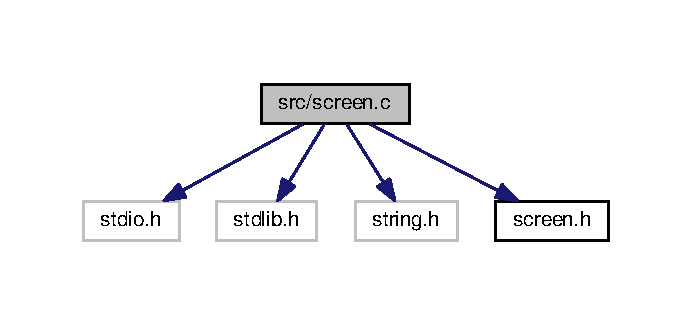
\includegraphics[width=332pt]{screen_8c__incl}
\end{center}
\end{figure}
\subsection*{Data Structures}
\begin{DoxyCompactItemize}
\item 
struct \hyperlink{struct__Area}{\+\_\+\+Area}
\begin{DoxyCompactList}\small\item\em screen of the game \end{DoxyCompactList}\end{DoxyCompactItemize}
\subsection*{Macros}
\begin{DoxyCompactItemize}
\item 
\#define \hyperlink{screen_8c_a3cfd3aa62338d12609f6d65bce97e9cd}{R\+O\+WS}~37
\item 
\#define \hyperlink{screen_8c_a06c6c391fc11d106e9909f0401b255b1}{C\+O\+L\+U\+M\+NS}~142
\item 
\#define \hyperlink{screen_8c_afba5c5b9f73273ce653f890bb64740b0}{T\+O\+T\+A\+L\+\_\+\+D\+A\+TA}~(\hyperlink{screen_8c_a3cfd3aa62338d12609f6d65bce97e9cd}{R\+O\+WS} $\ast$ \hyperlink{screen_8c_a06c6c391fc11d106e9909f0401b255b1}{C\+O\+L\+U\+M\+NS}) + 1
\item 
\#define \hyperlink{screen_8c_a5e7c78a2c827b39d4464f2fc84058f87}{B\+G\+\_\+\+C\+H\+AR}~\textquotesingle{}$\sim$\textquotesingle{}
\item 
\#define \hyperlink{screen_8c_a0bbf43d51e6cd6f7119cf1d0063a3a94}{F\+G\+\_\+\+C\+H\+AR}~\textquotesingle{} \textquotesingle{}
\item 
\#define \hyperlink{screen_8c_accdbea14ea06c15e271784368bd993e8}{P\+R\+O\+M\+PT}~\char`\"{} prompt\+:$>$ \char`\"{}
\item 
\#define \hyperlink{screen_8c_a28b37557462b06fbb08e707dc0ba2136}{A\+C\+C\+E\+SS}(d,  x,  y)~(d + ((y) $\ast$ \hyperlink{screen_8c_a06c6c391fc11d106e9909f0401b255b1}{C\+O\+L\+U\+M\+NS}) + (x))
\end{DoxyCompactItemize}
\subsection*{Functions}
\begin{DoxyCompactItemize}
\item 
int \hyperlink{screen_8c_ad1b32d3d54fea228f1ef0c73de4a3929}{screen\+\_\+area\+\_\+cursor\+\_\+is\+\_\+out\+\_\+of\+\_\+bounds} (\hyperlink{screen_8h_acfdfc42f6522d75fa3c16713afde8127}{Area} $\ast$area)
\begin{DoxyCompactList}\small\item\em checks if cursor is out of the limits \end{DoxyCompactList}\item 
void \hyperlink{screen_8c_a110e0b378730322f5a2f1dc91e65e2aa}{screen\+\_\+area\+\_\+scroll\+\_\+up} (\hyperlink{screen_8h_acfdfc42f6522d75fa3c16713afde8127}{Area} $\ast$area)
\begin{DoxyCompactList}\small\item\em scrolls up the screen area \end{DoxyCompactList}\item 
void \hyperlink{screen_8c_a55dedaa3b402fef825ceb6c3a957781d}{screen\+\_\+utils\+\_\+replaces\+\_\+special\+\_\+chars} (char $\ast$str)
\begin{DoxyCompactList}\small\item\em replaces special characters \end{DoxyCompactList}\item 
void \hyperlink{screen_8c_a9dbb6c251337c03c078dc330caee48d2}{screen\+\_\+init} ()
\begin{DoxyCompactList}\small\item\em initialises a new screen \end{DoxyCompactList}\item 
void \hyperlink{screen_8c_a3d6d82dde2bb4f3ddc4d276dabe313ef}{screen\+\_\+destroy} ()
\begin{DoxyCompactList}\small\item\em frees memory \end{DoxyCompactList}\item 
void \hyperlink{screen_8c_a3eaa0547a956d39b6c55c9593524e0d1}{screen\+\_\+paint} ()
\begin{DoxyCompactList}\small\item\em paints the screen \end{DoxyCompactList}\item 
void \hyperlink{screen_8c_a57b2f852be623dca59255306c1482eb2}{screen\+\_\+gets} (char $\ast$str)
\begin{DoxyCompactList}\small\item\em gets the data \end{DoxyCompactList}\item 
\hyperlink{screen_8h_acfdfc42f6522d75fa3c16713afde8127}{Area} $\ast$ \hyperlink{screen_8c_a194528bec3ed3b57618a8f2df9bea743}{screen\+\_\+area\+\_\+init} (int x, int y, int width, int height)
\begin{DoxyCompactList}\small\item\em creates new area \end{DoxyCompactList}\item 
void \hyperlink{screen_8c_aca5123ed5a7afb75e79c0001e5d1df4f}{screen\+\_\+area\+\_\+destroy} (\hyperlink{screen_8h_acfdfc42f6522d75fa3c16713afde8127}{Area} $\ast$area)
\begin{DoxyCompactList}\small\item\em frees memory \end{DoxyCompactList}\item 
void \hyperlink{screen_8c_a0950dc68cba3d491b909a8abaac1c666}{screen\+\_\+area\+\_\+clear} (\hyperlink{screen_8h_acfdfc42f6522d75fa3c16713afde8127}{Area} $\ast$area)
\begin{DoxyCompactList}\small\item\em clears the area \end{DoxyCompactList}\item 
void \hyperlink{screen_8c_af77fa9df4f7170e1e3bf1c6209b7f0c2}{screen\+\_\+area\+\_\+reset\+\_\+cursor} (\hyperlink{screen_8h_acfdfc42f6522d75fa3c16713afde8127}{Area} $\ast$area)
\begin{DoxyCompactList}\small\item\em resets cursor \end{DoxyCompactList}\item 
void \hyperlink{screen_8c_a4f4cd4c7899c096d6c90cc33de9a9814}{screen\+\_\+area\+\_\+puts} (\hyperlink{screen_8h_acfdfc42f6522d75fa3c16713afde8127}{Area} $\ast$area, char $\ast$str)
\begin{DoxyCompactList}\small\item\em puts area \end{DoxyCompactList}\end{DoxyCompactItemize}
\subsection*{Variables}
\begin{DoxyCompactItemize}
\item 
char $\ast$ \hyperlink{screen_8c_a34a5b96f7a2aa5db335b9fd09706cf0a}{\+\_\+\+\_\+data}
\end{DoxyCompactItemize}


\subsection{Detailed Description}
Defines the screen. 

\begin{DoxyAuthor}{Author}
Borja Pérez 
\end{DoxyAuthor}
\begin{DoxyVersion}{Version}
1.\+1 
\end{DoxyVersion}
\begin{DoxyDate}{Date}
29-\/04-\/2018 
\end{DoxyDate}


\subsection{Macro Definition Documentation}
\index{screen.\+c@{screen.\+c}!A\+C\+C\+E\+SS@{A\+C\+C\+E\+SS}}
\index{A\+C\+C\+E\+SS@{A\+C\+C\+E\+SS}!screen.\+c@{screen.\+c}}
\subsubsection[{\texorpdfstring{A\+C\+C\+E\+SS}{ACCESS}}]{\setlength{\rightskip}{0pt plus 5cm}\#define A\+C\+C\+E\+SS(
\begin{DoxyParamCaption}
\item[{}]{d, }
\item[{}]{x, }
\item[{}]{y}
\end{DoxyParamCaption}
)~(d + ((y) $\ast$ {\bf C\+O\+L\+U\+M\+NS}) + (x))}\hypertarget{screen_8c_a28b37557462b06fbb08e707dc0ba2136}{}\label{screen_8c_a28b37557462b06fbb08e707dc0ba2136}
access to the screen \index{screen.\+c@{screen.\+c}!B\+G\+\_\+\+C\+H\+AR@{B\+G\+\_\+\+C\+H\+AR}}
\index{B\+G\+\_\+\+C\+H\+AR@{B\+G\+\_\+\+C\+H\+AR}!screen.\+c@{screen.\+c}}
\subsubsection[{\texorpdfstring{B\+G\+\_\+\+C\+H\+AR}{BG_CHAR}}]{\setlength{\rightskip}{0pt plus 5cm}\#define B\+G\+\_\+\+C\+H\+AR~\textquotesingle{}$\sim$\textquotesingle{}}\hypertarget{screen_8c_a5e7c78a2c827b39d4464f2fc84058f87}{}\label{screen_8c_a5e7c78a2c827b39d4464f2fc84058f87}
action to make \index{screen.\+c@{screen.\+c}!C\+O\+L\+U\+M\+NS@{C\+O\+L\+U\+M\+NS}}
\index{C\+O\+L\+U\+M\+NS@{C\+O\+L\+U\+M\+NS}!screen.\+c@{screen.\+c}}
\subsubsection[{\texorpdfstring{C\+O\+L\+U\+M\+NS}{COLUMNS}}]{\setlength{\rightskip}{0pt plus 5cm}\#define C\+O\+L\+U\+M\+NS~142}\hypertarget{screen_8c_a06c6c391fc11d106e9909f0401b255b1}{}\label{screen_8c_a06c6c391fc11d106e9909f0401b255b1}
columns of the game \index{screen.\+c@{screen.\+c}!F\+G\+\_\+\+C\+H\+AR@{F\+G\+\_\+\+C\+H\+AR}}
\index{F\+G\+\_\+\+C\+H\+AR@{F\+G\+\_\+\+C\+H\+AR}!screen.\+c@{screen.\+c}}
\subsubsection[{\texorpdfstring{F\+G\+\_\+\+C\+H\+AR}{FG_CHAR}}]{\setlength{\rightskip}{0pt plus 5cm}\#define F\+G\+\_\+\+C\+H\+AR~\textquotesingle{} \textquotesingle{}}\hypertarget{screen_8c_a0bbf43d51e6cd6f7119cf1d0063a3a94}{}\label{screen_8c_a0bbf43d51e6cd6f7119cf1d0063a3a94}
blank space \index{screen.\+c@{screen.\+c}!P\+R\+O\+M\+PT@{P\+R\+O\+M\+PT}}
\index{P\+R\+O\+M\+PT@{P\+R\+O\+M\+PT}!screen.\+c@{screen.\+c}}
\subsubsection[{\texorpdfstring{P\+R\+O\+M\+PT}{PROMPT}}]{\setlength{\rightskip}{0pt plus 5cm}\#define P\+R\+O\+M\+PT~\char`\"{} prompt\+:$>$ \char`\"{}}\hypertarget{screen_8c_accdbea14ea06c15e271784368bd993e8}{}\label{screen_8c_accdbea14ea06c15e271784368bd993e8}
action to make \index{screen.\+c@{screen.\+c}!R\+O\+WS@{R\+O\+WS}}
\index{R\+O\+WS@{R\+O\+WS}!screen.\+c@{screen.\+c}}
\subsubsection[{\texorpdfstring{R\+O\+WS}{ROWS}}]{\setlength{\rightskip}{0pt plus 5cm}\#define R\+O\+WS~37}\hypertarget{screen_8c_a3cfd3aa62338d12609f6d65bce97e9cd}{}\label{screen_8c_a3cfd3aa62338d12609f6d65bce97e9cd}
rows of the game \index{screen.\+c@{screen.\+c}!T\+O\+T\+A\+L\+\_\+\+D\+A\+TA@{T\+O\+T\+A\+L\+\_\+\+D\+A\+TA}}
\index{T\+O\+T\+A\+L\+\_\+\+D\+A\+TA@{T\+O\+T\+A\+L\+\_\+\+D\+A\+TA}!screen.\+c@{screen.\+c}}
\subsubsection[{\texorpdfstring{T\+O\+T\+A\+L\+\_\+\+D\+A\+TA}{TOTAL_DATA}}]{\setlength{\rightskip}{0pt plus 5cm}\#define T\+O\+T\+A\+L\+\_\+\+D\+A\+TA~({\bf R\+O\+WS} $\ast$ {\bf C\+O\+L\+U\+M\+NS}) + 1}\hypertarget{screen_8c_afba5c5b9f73273ce653f890bb64740b0}{}\label{screen_8c_afba5c5b9f73273ce653f890bb64740b0}
total data of the game 

\subsection{Function Documentation}
\index{screen.\+c@{screen.\+c}!screen\+\_\+area\+\_\+clear@{screen\+\_\+area\+\_\+clear}}
\index{screen\+\_\+area\+\_\+clear@{screen\+\_\+area\+\_\+clear}!screen.\+c@{screen.\+c}}
\subsubsection[{\texorpdfstring{screen\+\_\+area\+\_\+clear(\+Area $\ast$area)}{screen_area_clear(Area *area)}}]{\setlength{\rightskip}{0pt plus 5cm}void screen\+\_\+area\+\_\+clear (
\begin{DoxyParamCaption}
\item[{{\bf Area} $\ast$}]{area}
\end{DoxyParamCaption}
)}\hypertarget{screen_8c_a0950dc68cba3d491b909a8abaac1c666}{}\label{screen_8c_a0950dc68cba3d491b909a8abaac1c666}


clears the area 

Deletes everthing in the area, leaving it as if it was just created.

\begin{DoxyAuthor}{Author}
Andrés Mena 
\end{DoxyAuthor}

\begin{DoxyParams}{Parameters}
{\em area} & pointer to area. \\
\hline
\end{DoxyParams}
\begin{DoxyReturn}{Returns}
void. 
\end{DoxyReturn}
\index{screen.\+c@{screen.\+c}!screen\+\_\+area\+\_\+cursor\+\_\+is\+\_\+out\+\_\+of\+\_\+bounds@{screen\+\_\+area\+\_\+cursor\+\_\+is\+\_\+out\+\_\+of\+\_\+bounds}}
\index{screen\+\_\+area\+\_\+cursor\+\_\+is\+\_\+out\+\_\+of\+\_\+bounds@{screen\+\_\+area\+\_\+cursor\+\_\+is\+\_\+out\+\_\+of\+\_\+bounds}!screen.\+c@{screen.\+c}}
\subsubsection[{\texorpdfstring{screen\+\_\+area\+\_\+cursor\+\_\+is\+\_\+out\+\_\+of\+\_\+bounds(\+Area $\ast$area)}{screen_area_cursor_is_out_of_bounds(Area *area)}}]{\setlength{\rightskip}{0pt plus 5cm}int screen\+\_\+area\+\_\+cursor\+\_\+is\+\_\+out\+\_\+of\+\_\+bounds (
\begin{DoxyParamCaption}
\item[{{\bf Area} $\ast$}]{area}
\end{DoxyParamCaption}
)}\hypertarget{screen_8c_ad1b32d3d54fea228f1ef0c73de4a3929}{}\label{screen_8c_ad1b32d3d54fea228f1ef0c73de4a3929}


checks if cursor is out of the limits 

\begin{DoxyAuthor}{Author}
Andrés Mena 
\end{DoxyAuthor}

\begin{DoxyParams}{Parameters}
{\em area} & pointer to area \\
\hline
\end{DoxyParams}
\begin{DoxyReturn}{Returns}
int (data of the cursor). 
\end{DoxyReturn}
\index{screen.\+c@{screen.\+c}!screen\+\_\+area\+\_\+destroy@{screen\+\_\+area\+\_\+destroy}}
\index{screen\+\_\+area\+\_\+destroy@{screen\+\_\+area\+\_\+destroy}!screen.\+c@{screen.\+c}}
\subsubsection[{\texorpdfstring{screen\+\_\+area\+\_\+destroy(\+Area $\ast$area)}{screen_area_destroy(Area *area)}}]{\setlength{\rightskip}{0pt plus 5cm}void screen\+\_\+area\+\_\+destroy (
\begin{DoxyParamCaption}
\item[{{\bf Area} $\ast$}]{area}
\end{DoxyParamCaption}
)}\hypertarget{screen_8c_aca5123ed5a7afb75e79c0001e5d1df4f}{}\label{screen_8c_aca5123ed5a7afb75e79c0001e5d1df4f}


frees memory 

Receives pointer to area and frees the memory it occupied.

\begin{DoxyAuthor}{Author}
Andrés Mena 
\end{DoxyAuthor}

\begin{DoxyParams}{Parameters}
{\em area} & pointer to area. \\
\hline
\end{DoxyParams}
\begin{DoxyReturn}{Returns}
void. 
\end{DoxyReturn}
\index{screen.\+c@{screen.\+c}!screen\+\_\+area\+\_\+init@{screen\+\_\+area\+\_\+init}}
\index{screen\+\_\+area\+\_\+init@{screen\+\_\+area\+\_\+init}!screen.\+c@{screen.\+c}}
\subsubsection[{\texorpdfstring{screen\+\_\+area\+\_\+init(int x, int y, int width, int height)}{screen_area_init(int x, int y, int width, int height)}}]{\setlength{\rightskip}{0pt plus 5cm}{\bf Area}$\ast$ screen\+\_\+area\+\_\+init (
\begin{DoxyParamCaption}
\item[{int}]{x, }
\item[{int}]{y, }
\item[{int}]{width, }
\item[{int}]{height}
\end{DoxyParamCaption}
)}\hypertarget{screen_8c_a194528bec3ed3b57618a8f2df9bea743}{}\label{screen_8c_a194528bec3ed3b57618a8f2df9bea743}


creates new area 

Allocates memory for an area, using x and y coordinates as a start point and width and height as the size.

\begin{DoxyAuthor}{Author}
Andrés Mena 
\end{DoxyAuthor}

\begin{DoxyParams}{Parameters}
{\em x} & int (coord x). \\
\hline
{\em y} & int (coord y). \\
\hline
{\em width} & int (width of the area). \\
\hline
{\em height} & int (height of the area). \\
\hline
\end{DoxyParams}
\begin{DoxyReturn}{Returns}
pointer to area. 
\end{DoxyReturn}
\index{screen.\+c@{screen.\+c}!screen\+\_\+area\+\_\+puts@{screen\+\_\+area\+\_\+puts}}
\index{screen\+\_\+area\+\_\+puts@{screen\+\_\+area\+\_\+puts}!screen.\+c@{screen.\+c}}
\subsubsection[{\texorpdfstring{screen\+\_\+area\+\_\+puts(\+Area $\ast$area, char $\ast$str)}{screen_area_puts(Area *area, char *str)}}]{\setlength{\rightskip}{0pt plus 5cm}void screen\+\_\+area\+\_\+puts (
\begin{DoxyParamCaption}
\item[{{\bf Area} $\ast$}]{area, }
\item[{char $\ast$}]{str}
\end{DoxyParamCaption}
)}\hypertarget{screen_8c_a4f4cd4c7899c096d6c90cc33de9a9814}{}\label{screen_8c_a4f4cd4c7899c096d6c90cc33de9a9814}


puts area 

Starts a new line in the area.

\begin{DoxyAuthor}{Author}
Andrés Mena 
\end{DoxyAuthor}

\begin{DoxyParams}{Parameters}
{\em area} & pointer to area. \\
\hline
{\em str} & char. \\
\hline
\end{DoxyParams}
\begin{DoxyReturn}{Returns}
void. 
\end{DoxyReturn}
\index{screen.\+c@{screen.\+c}!screen\+\_\+area\+\_\+reset\+\_\+cursor@{screen\+\_\+area\+\_\+reset\+\_\+cursor}}
\index{screen\+\_\+area\+\_\+reset\+\_\+cursor@{screen\+\_\+area\+\_\+reset\+\_\+cursor}!screen.\+c@{screen.\+c}}
\subsubsection[{\texorpdfstring{screen\+\_\+area\+\_\+reset\+\_\+cursor(\+Area $\ast$area)}{screen_area_reset_cursor(Area *area)}}]{\setlength{\rightskip}{0pt plus 5cm}void screen\+\_\+area\+\_\+reset\+\_\+cursor (
\begin{DoxyParamCaption}
\item[{{\bf Area} $\ast$}]{area}
\end{DoxyParamCaption}
)}\hypertarget{screen_8c_af77fa9df4f7170e1e3bf1c6209b7f0c2}{}\label{screen_8c_af77fa9df4f7170e1e3bf1c6209b7f0c2}


resets cursor 

Resets the cursor, leaving it in the 0,0 coordinates of the area.

\begin{DoxyAuthor}{Author}
Andrés Mena 
\end{DoxyAuthor}

\begin{DoxyParams}{Parameters}
{\em area} & pointer to area. \\
\hline
\end{DoxyParams}
\begin{DoxyReturn}{Returns}
void. 
\end{DoxyReturn}
\index{screen.\+c@{screen.\+c}!screen\+\_\+area\+\_\+scroll\+\_\+up@{screen\+\_\+area\+\_\+scroll\+\_\+up}}
\index{screen\+\_\+area\+\_\+scroll\+\_\+up@{screen\+\_\+area\+\_\+scroll\+\_\+up}!screen.\+c@{screen.\+c}}
\subsubsection[{\texorpdfstring{screen\+\_\+area\+\_\+scroll\+\_\+up(\+Area $\ast$area)}{screen_area_scroll_up(Area *area)}}]{\setlength{\rightskip}{0pt plus 5cm}void screen\+\_\+area\+\_\+scroll\+\_\+up (
\begin{DoxyParamCaption}
\item[{{\bf Area} $\ast$}]{area}
\end{DoxyParamCaption}
)}\hypertarget{screen_8c_a110e0b378730322f5a2f1dc91e65e2aa}{}\label{screen_8c_a110e0b378730322f5a2f1dc91e65e2aa}


scrolls up the screen area 

\begin{DoxyAuthor}{Author}
Andrés Mena 
\end{DoxyAuthor}

\begin{DoxyParams}{Parameters}
{\em area} & pointer to area \\
\hline
\end{DoxyParams}
\begin{DoxyReturn}{Returns}
void function. 
\end{DoxyReturn}
\index{screen.\+c@{screen.\+c}!screen\+\_\+destroy@{screen\+\_\+destroy}}
\index{screen\+\_\+destroy@{screen\+\_\+destroy}!screen.\+c@{screen.\+c}}
\subsubsection[{\texorpdfstring{screen\+\_\+destroy()}{screen_destroy()}}]{\setlength{\rightskip}{0pt plus 5cm}void screen\+\_\+destroy (
\begin{DoxyParamCaption}
{}
\end{DoxyParamCaption}
)}\hypertarget{screen_8c_a3d6d82dde2bb4f3ddc4d276dabe313ef}{}\label{screen_8c_a3d6d82dde2bb4f3ddc4d276dabe313ef}


frees memory 

frees the data that screen occupied.

\begin{DoxyAuthor}{Author}
Andrés Mena 
\end{DoxyAuthor}
\begin{DoxyReturn}{Returns}
void. 
\end{DoxyReturn}
\index{screen.\+c@{screen.\+c}!screen\+\_\+gets@{screen\+\_\+gets}}
\index{screen\+\_\+gets@{screen\+\_\+gets}!screen.\+c@{screen.\+c}}
\subsubsection[{\texorpdfstring{screen\+\_\+gets(char $\ast$str)}{screen_gets(char *str)}}]{\setlength{\rightskip}{0pt plus 5cm}void screen\+\_\+gets (
\begin{DoxyParamCaption}
\item[{char $\ast$}]{str}
\end{DoxyParamCaption}
)}\hypertarget{screen_8c_a57b2f852be623dca59255306c1482eb2}{}\label{screen_8c_a57b2f852be623dca59255306c1482eb2}


gets the data 

Gets the data typed in the ingame console (commands).

\begin{DoxyAuthor}{Author}
Andrés Mena 
\end{DoxyAuthor}

\begin{DoxyParams}{Parameters}
{\em str} & char (data of the console). \\
\hline
\end{DoxyParams}
\begin{DoxyReturn}{Returns}
void. 
\end{DoxyReturn}
\index{screen.\+c@{screen.\+c}!screen\+\_\+init@{screen\+\_\+init}}
\index{screen\+\_\+init@{screen\+\_\+init}!screen.\+c@{screen.\+c}}
\subsubsection[{\texorpdfstring{screen\+\_\+init()}{screen_init()}}]{\setlength{\rightskip}{0pt plus 5cm}void screen\+\_\+init (
\begin{DoxyParamCaption}
{}
\end{DoxyParamCaption}
)}\hypertarget{screen_8c_a9dbb6c251337c03c078dc330caee48d2}{}\label{screen_8c_a9dbb6c251337c03c078dc330caee48d2}


initialises a new screen 

Destroys any previous screen and allocates memory for a new one.

\begin{DoxyAuthor}{Author}
Andrés Mena 
\end{DoxyAuthor}
\begin{DoxyReturn}{Returns}
void. 
\end{DoxyReturn}
\index{screen.\+c@{screen.\+c}!screen\+\_\+paint@{screen\+\_\+paint}}
\index{screen\+\_\+paint@{screen\+\_\+paint}!screen.\+c@{screen.\+c}}
\subsubsection[{\texorpdfstring{screen\+\_\+paint()}{screen_paint()}}]{\setlength{\rightskip}{0pt plus 5cm}void screen\+\_\+paint (
\begin{DoxyParamCaption}
{}
\end{DoxyParamCaption}
)}\hypertarget{screen_8c_a3eaa0547a956d39b6c55c9593524e0d1}{}\label{screen_8c_a3eaa0547a956d39b6c55c9593524e0d1}


paints the screen 

Prints a screen in the console.

\begin{DoxyAuthor}{Author}
Andrés Mena 
\end{DoxyAuthor}
\begin{DoxyReturn}{Returns}
void. 
\end{DoxyReturn}
\index{screen.\+c@{screen.\+c}!screen\+\_\+utils\+\_\+replaces\+\_\+special\+\_\+chars@{screen\+\_\+utils\+\_\+replaces\+\_\+special\+\_\+chars}}
\index{screen\+\_\+utils\+\_\+replaces\+\_\+special\+\_\+chars@{screen\+\_\+utils\+\_\+replaces\+\_\+special\+\_\+chars}!screen.\+c@{screen.\+c}}
\subsubsection[{\texorpdfstring{screen\+\_\+utils\+\_\+replaces\+\_\+special\+\_\+chars(char $\ast$str)}{screen_utils_replaces_special_chars(char *str)}}]{\setlength{\rightskip}{0pt plus 5cm}void screen\+\_\+utils\+\_\+replaces\+\_\+special\+\_\+chars (
\begin{DoxyParamCaption}
\item[{char $\ast$}]{str}
\end{DoxyParamCaption}
)}\hypertarget{screen_8c_a55dedaa3b402fef825ceb6c3a957781d}{}\label{screen_8c_a55dedaa3b402fef825ceb6c3a957781d}


replaces special characters 

\begin{DoxyAuthor}{Author}
Andrés Mena 
\end{DoxyAuthor}

\begin{DoxyParams}{Parameters}
{\em str} & (char string). \\
\hline
\end{DoxyParams}
\begin{DoxyReturn}{Returns}
void function. 
\end{DoxyReturn}


\subsection{Variable Documentation}
\index{screen.\+c@{screen.\+c}!\+\_\+\+\_\+data@{\+\_\+\+\_\+data}}
\index{\+\_\+\+\_\+data@{\+\_\+\+\_\+data}!screen.\+c@{screen.\+c}}
\subsubsection[{\texorpdfstring{\+\_\+\+\_\+data}{__data}}]{\setlength{\rightskip}{0pt plus 5cm}char$\ast$ \+\_\+\+\_\+data}\hypertarget{screen_8c_a34a5b96f7a2aa5db335b9fd09706cf0a}{}\label{screen_8c_a34a5b96f7a2aa5db335b9fd09706cf0a}
data of the game 
\hypertarget{space_8c}{}\section{src/space.c File Reference}
\label{space_8c}\index{src/space.\+c@{src/space.\+c}}


Defines the space related functions.  


{\ttfamily \#include $<$stdio.\+h$>$}\\*
{\ttfamily \#include $<$stdlib.\+h$>$}\\*
{\ttfamily \#include $<$string.\+h$>$}\\*
{\ttfamily \#include \char`\"{}types.\+h\char`\"{}}\\*
{\ttfamily \#include \char`\"{}space.\+h\char`\"{}}\\*
{\ttfamily \#include \char`\"{}link.\+h\char`\"{}}\\*
Include dependency graph for space.\+c\+:
\nopagebreak
\begin{figure}[H]
\begin{center}
\leavevmode
\includegraphics[width=350pt]{space_8c__incl}
\end{center}
\end{figure}
\subsection*{Data Structures}
\begin{DoxyCompactItemize}
\item 
struct \hyperlink{struct__Space}{\+\_\+\+Space}
\begin{DoxyCompactList}\small\item\em spaces of the game \end{DoxyCompactList}\end{DoxyCompactItemize}
\subsection*{Functions}
\begin{DoxyCompactItemize}
\item 
char $\ast$ \hyperlink{space_8c_a82ebe192d237170b770156f2b2dd0ede}{space\+\_\+get\+\_\+gdesc\+\_\+line} (\hyperlink{space_8h_a67533ffc2b70463baecc38fb0629bbfc}{Space} $\ast$s, int line)
\begin{DoxyCompactList}\small\item\em gets description \end{DoxyCompactList}\item 
\hyperlink{types_8h_a32c27cc471df37f4fc818d65de0a56c4}{S\+T\+A\+T\+US} \hyperlink{space_8c_a3d92143458bc73e064379d54b363ffb1}{space\+\_\+set\+\_\+gdesc\+\_\+line} (\hyperlink{space_8h_a67533ffc2b70463baecc38fb0629bbfc}{Space} $\ast$s, int line, char $\ast$c)
\begin{DoxyCompactList}\small\item\em sets description \end{DoxyCompactList}\item 
\hyperlink{space_8h_a67533ffc2b70463baecc38fb0629bbfc}{Space} $\ast$ \hyperlink{space_8c_a162866fcea156b800fd546d0ffd271c9}{space\+\_\+create} (\hyperlink{types_8h_a845e604fb28f7e3d97549da3448149d3}{Id} id)
\begin{DoxyCompactList}\small\item\em allocates memory for a new space \end{DoxyCompactList}\item 
\hyperlink{types_8h_a32c27cc471df37f4fc818d65de0a56c4}{S\+T\+A\+T\+US} \hyperlink{space_8c_a5c70c70398923693ddbe4dfac8d72a0d}{space\+\_\+destroy} (\hyperlink{space_8h_a67533ffc2b70463baecc38fb0629bbfc}{Space} $\ast$space)
\begin{DoxyCompactList}\small\item\em frees memory \end{DoxyCompactList}\item 
\hyperlink{types_8h_a32c27cc471df37f4fc818d65de0a56c4}{S\+T\+A\+T\+US} \hyperlink{space_8c_aab5b468f9822ab78dbe16d1321870d93}{space\+\_\+set\+\_\+name} (\hyperlink{space_8h_a67533ffc2b70463baecc38fb0629bbfc}{Space} $\ast$space, char $\ast$name)
\begin{DoxyCompactList}\small\item\em sets the name of a space \end{DoxyCompactList}\item 
\hyperlink{types_8h_a32c27cc471df37f4fc818d65de0a56c4}{S\+T\+A\+T\+US} \hyperlink{space_8c_a52d48979efbb5ba49c0988ddffc33769}{space\+\_\+set\+\_\+short\+\_\+description} (\hyperlink{space_8h_a67533ffc2b70463baecc38fb0629bbfc}{Space} $\ast$space, char $\ast$description)
\begin{DoxyCompactList}\small\item\em sets description \end{DoxyCompactList}\item 
char $\ast$ \hyperlink{space_8c_aa389d6b22e635bb9d2f1a18d9cd0d1cb}{space\+\_\+get\+\_\+short\+\_\+description} (\hyperlink{space_8h_a67533ffc2b70463baecc38fb0629bbfc}{Space} $\ast$space)
\begin{DoxyCompactList}\small\item\em gets description \end{DoxyCompactList}\item 
\hyperlink{types_8h_a32c27cc471df37f4fc818d65de0a56c4}{S\+T\+A\+T\+US} \hyperlink{space_8c_adaea1c731830282c8a29f3477a93ac2e}{space\+\_\+set\+\_\+long\+\_\+description} (\hyperlink{space_8h_a67533ffc2b70463baecc38fb0629bbfc}{Space} $\ast$space, char $\ast$description)
\begin{DoxyCompactList}\small\item\em sets description \end{DoxyCompactList}\item 
char $\ast$ \hyperlink{space_8c_a5c38e8f0892b1683b4f058d17ea1549d}{space\+\_\+get\+\_\+long\+\_\+description} (\hyperlink{space_8h_a67533ffc2b70463baecc38fb0629bbfc}{Space} $\ast$space)
\begin{DoxyCompactList}\small\item\em gets description \end{DoxyCompactList}\item 
\hyperlink{types_8h_a32c27cc471df37f4fc818d65de0a56c4}{S\+T\+A\+T\+US} \hyperlink{space_8c_a9e6e3e3bac4996ac6b8bd555e52bfb26}{space\+\_\+set\+\_\+north} (\hyperlink{space_8h_a67533ffc2b70463baecc38fb0629bbfc}{Space} $\ast$space, \hyperlink{types_8h_a845e604fb28f7e3d97549da3448149d3}{Id} id)
\begin{DoxyCompactList}\small\item\em sets location of spaces \end{DoxyCompactList}\item 
\hyperlink{types_8h_a32c27cc471df37f4fc818d65de0a56c4}{S\+T\+A\+T\+US} \hyperlink{space_8c_a422ab9f220b4c471c44256a27377de1a}{space\+\_\+set\+\_\+south} (\hyperlink{space_8h_a67533ffc2b70463baecc38fb0629bbfc}{Space} $\ast$space, \hyperlink{types_8h_a845e604fb28f7e3d97549da3448149d3}{Id} id)
\begin{DoxyCompactList}\small\item\em sets location of spaces \end{DoxyCompactList}\item 
\hyperlink{types_8h_a32c27cc471df37f4fc818d65de0a56c4}{S\+T\+A\+T\+US} \hyperlink{space_8c_a860a8f3e0227955ad56d1a12f0bdc44a}{space\+\_\+set\+\_\+east} (\hyperlink{space_8h_a67533ffc2b70463baecc38fb0629bbfc}{Space} $\ast$space, \hyperlink{types_8h_a845e604fb28f7e3d97549da3448149d3}{Id} id)
\begin{DoxyCompactList}\small\item\em sets location of spaces \end{DoxyCompactList}\item 
\hyperlink{types_8h_a32c27cc471df37f4fc818d65de0a56c4}{S\+T\+A\+T\+US} \hyperlink{space_8c_ad44b14cb38902cf31fa1f341beaab0db}{space\+\_\+set\+\_\+west} (\hyperlink{space_8h_a67533ffc2b70463baecc38fb0629bbfc}{Space} $\ast$space, \hyperlink{types_8h_a845e604fb28f7e3d97549da3448149d3}{Id} id)
\begin{DoxyCompactList}\small\item\em sets location of spaces \end{DoxyCompactList}\item 
\hyperlink{types_8h_a32c27cc471df37f4fc818d65de0a56c4}{S\+T\+A\+T\+US} \hyperlink{space_8c_aa2707bdca8fd356ed8d15fd48e820a4f}{space\+\_\+set\+\_\+up} (\hyperlink{space_8h_a67533ffc2b70463baecc38fb0629bbfc}{Space} $\ast$space, \hyperlink{types_8h_a845e604fb28f7e3d97549da3448149d3}{Id} id)
\begin{DoxyCompactList}\small\item\em sets location of spaces \end{DoxyCompactList}\item 
\hyperlink{types_8h_a32c27cc471df37f4fc818d65de0a56c4}{S\+T\+A\+T\+US} \hyperlink{space_8c_ae5b9fef52456ffccffbd73f882a56d23}{space\+\_\+set\+\_\+down} (\hyperlink{space_8h_a67533ffc2b70463baecc38fb0629bbfc}{Space} $\ast$space, \hyperlink{types_8h_a845e604fb28f7e3d97549da3448149d3}{Id} id)
\begin{DoxyCompactList}\small\item\em sets location of spaces \end{DoxyCompactList}\item 
\hyperlink{types_8h_a32c27cc471df37f4fc818d65de0a56c4}{S\+T\+A\+T\+US} \hyperlink{space_8c_ab2803dc6dee6ca4360860b0b9a66b34e}{space\+\_\+set\+\_\+iluminate} (\hyperlink{space_8h_a67533ffc2b70463baecc38fb0629bbfc}{Space} $\ast$space, \hyperlink{types_8h_a3e5b8192e7d9ffaf3542f1210aec18dd}{B\+O\+OL} iluminate)
\begin{DoxyCompactList}\small\item\em sets ilumination \end{DoxyCompactList}\item 
\hyperlink{types_8h_a3e5b8192e7d9ffaf3542f1210aec18dd}{B\+O\+OL} \hyperlink{space_8c_aef4fa60815bc64dde3c16855aa470f63}{space\+\_\+get\+\_\+iluminate} (\hyperlink{space_8h_a67533ffc2b70463baecc38fb0629bbfc}{Space} $\ast$space)
\begin{DoxyCompactList}\small\item\em returns the iluminated space \end{DoxyCompactList}\item 
\hyperlink{types_8h_a32c27cc471df37f4fc818d65de0a56c4}{S\+T\+A\+T\+US} \hyperlink{space_8c_a97f27baaafef8eb986d167788dc84bec}{space\+\_\+set\+\_\+object} (\hyperlink{space_8h_a67533ffc2b70463baecc38fb0629bbfc}{Space} $\ast$space, \hyperlink{object_8h_a7f8bbcda919b65ce67f92fba08e0212f}{Object} $\ast$o)
\begin{DoxyCompactList}\small\item\em sets an object for a space \end{DoxyCompactList}\item 
int \hyperlink{space_8c_ab39ec663cd2f64cd8406f5ba6f5493ea}{space\+\_\+get\+\_\+object\+\_\+number} (\hyperlink{space_8h_a67533ffc2b70463baecc38fb0629bbfc}{Space} $\ast$space)
\begin{DoxyCompactList}\small\item\em gets number \end{DoxyCompactList}\item 
const char $\ast$ \hyperlink{space_8c_a310c540cd6e11073f7328add1f927001}{space\+\_\+get\+\_\+name} (\hyperlink{space_8h_a67533ffc2b70463baecc38fb0629bbfc}{Space} $\ast$space)
\begin{DoxyCompactList}\small\item\em gets the name of a space \end{DoxyCompactList}\item 
\hyperlink{types_8h_a845e604fb28f7e3d97549da3448149d3}{Id} \hyperlink{space_8c_ac8ddfd0d8692fd852ee49698c446cb50}{space\+\_\+get\+\_\+id} (\hyperlink{space_8h_a67533ffc2b70463baecc38fb0629bbfc}{Space} $\ast$space)
\begin{DoxyCompactList}\small\item\em gets the id of a space \end{DoxyCompactList}\item 
\hyperlink{types_8h_a845e604fb28f7e3d97549da3448149d3}{Id} \hyperlink{space_8c_ad331fba774897900f615d9d2e8d81a90}{space\+\_\+get\+\_\+north} (\hyperlink{space_8h_a67533ffc2b70463baecc38fb0629bbfc}{Space} $\ast$space)
\begin{DoxyCompactList}\small\item\em gets location of spaces \end{DoxyCompactList}\item 
\hyperlink{types_8h_a845e604fb28f7e3d97549da3448149d3}{Id} \hyperlink{space_8c_a9b86e1335c423eaad832e50d4c12cf1f}{space\+\_\+get\+\_\+south} (\hyperlink{space_8h_a67533ffc2b70463baecc38fb0629bbfc}{Space} $\ast$space)
\begin{DoxyCompactList}\small\item\em gets location of spaces \end{DoxyCompactList}\item 
\hyperlink{types_8h_a845e604fb28f7e3d97549da3448149d3}{Id} \hyperlink{space_8c_a978a22b77f74bb2dab68a00571abbe0b}{space\+\_\+get\+\_\+east} (\hyperlink{space_8h_a67533ffc2b70463baecc38fb0629bbfc}{Space} $\ast$space)
\begin{DoxyCompactList}\small\item\em gets location of spaces \end{DoxyCompactList}\item 
\hyperlink{types_8h_a845e604fb28f7e3d97549da3448149d3}{Id} \hyperlink{space_8c_af495ebfd5d13eba1a48cebd10992a17f}{space\+\_\+get\+\_\+west} (\hyperlink{space_8h_a67533ffc2b70463baecc38fb0629bbfc}{Space} $\ast$space)
\begin{DoxyCompactList}\small\item\em gets location of spaces \end{DoxyCompactList}\item 
\hyperlink{types_8h_a845e604fb28f7e3d97549da3448149d3}{Id} \hyperlink{space_8c_a174a988b899d5a0db889a31b70763c9c}{space\+\_\+get\+\_\+up} (\hyperlink{space_8h_a67533ffc2b70463baecc38fb0629bbfc}{Space} $\ast$space)
\begin{DoxyCompactList}\small\item\em gets location of spaces \end{DoxyCompactList}\item 
\hyperlink{types_8h_a845e604fb28f7e3d97549da3448149d3}{Id} \hyperlink{space_8c_ab269eab72b9ea7254044b34b1c177602}{space\+\_\+get\+\_\+down} (\hyperlink{space_8h_a67533ffc2b70463baecc38fb0629bbfc}{Space} $\ast$space)
\begin{DoxyCompactList}\small\item\em gets location of spaces \end{DoxyCompactList}\item 
\hyperlink{set_8h_a6d3b7f7c92cbb4577ef3ef7ddbf93161}{Set} $\ast$ \hyperlink{space_8c_ab24abae4e127bf0bca596cd71ba3aad6}{space\+\_\+get\+\_\+object} (\hyperlink{space_8h_a67533ffc2b70463baecc38fb0629bbfc}{Space} $\ast$space)
\begin{DoxyCompactList}\small\item\em gets an object from a space \end{DoxyCompactList}\item 
\hyperlink{types_8h_a32c27cc471df37f4fc818d65de0a56c4}{S\+T\+A\+T\+US} \hyperlink{space_8c_ab7c8deb146adb40f1c07660e5442650e}{space\+\_\+object\+\_\+destroy} (\hyperlink{space_8h_a67533ffc2b70463baecc38fb0629bbfc}{Space} $\ast$s, \hyperlink{types_8h_a845e604fb28f7e3d97549da3448149d3}{Id} id)
\begin{DoxyCompactList}\small\item\em frees memory \end{DoxyCompactList}\item 
\hyperlink{types_8h_a32c27cc471df37f4fc818d65de0a56c4}{S\+T\+A\+T\+US} \hyperlink{space_8c_a18eca058da6cdf20ae5eda9d122d992e}{space\+\_\+print} (\hyperlink{space_8h_a67533ffc2b70463baecc38fb0629bbfc}{Space} $\ast$space)
\begin{DoxyCompactList}\small\item\em prints the spaces \end{DoxyCompactList}\item 
\hyperlink{types_8h_a3e5b8192e7d9ffaf3542f1210aec18dd}{B\+O\+OL} \hyperlink{space_8c_a0642818ac93d8696fa46f371b8c2801d}{space\+\_\+is\+\_\+linked} (\hyperlink{space_8h_a67533ffc2b70463baecc38fb0629bbfc}{Space} $\ast$s)
\begin{DoxyCompactList}\small\item\em checks if space is linked \end{DoxyCompactList}\end{DoxyCompactItemize}


\subsection{Detailed Description}
Defines the space related functions. 

Sets the new functionality of the space module that will allow is incorporate other new complements created.

\begin{DoxyAuthor}{Author}
Dan Roife 
\end{DoxyAuthor}
\begin{DoxyVersion}{Version}
1.\+1 
\end{DoxyVersion}
\begin{DoxyDate}{Date}
08-\/04-\/2018 
\end{DoxyDate}


\subsection{Function Documentation}
\index{space.\+c@{space.\+c}!space\+\_\+create@{space\+\_\+create}}
\index{space\+\_\+create@{space\+\_\+create}!space.\+c@{space.\+c}}
\subsubsection[{\texorpdfstring{space\+\_\+create(\+Id id)}{space_create(Id id)}}]{\setlength{\rightskip}{0pt plus 5cm}{\bf Space}$\ast$ space\+\_\+create (
\begin{DoxyParamCaption}
\item[{{\bf Id}}]{id}
\end{DoxyParamCaption}
)}\hypertarget{space_8c_a162866fcea156b800fd546d0ffd271c9}{}\label{space_8c_a162866fcea156b800fd546d0ffd271c9}


allocates memory for a new space 

It creates a new space initializing the variables of the structure, checks is something goes wrong and if it does go wrong, returns N\+U\+LL.

\begin{DoxyAuthor}{Author}
Dan Roife 
\end{DoxyAuthor}

\begin{DoxyParams}{Parameters}
{\em id} & (long int). \\
\hline
\end{DoxyParams}
\begin{DoxyReturn}{Returns}
Pointer to space, N\+U\+LL if something goes wrong. 
\end{DoxyReturn}
\index{space.\+c@{space.\+c}!space\+\_\+destroy@{space\+\_\+destroy}}
\index{space\+\_\+destroy@{space\+\_\+destroy}!space.\+c@{space.\+c}}
\subsubsection[{\texorpdfstring{space\+\_\+destroy(\+Space $\ast$space)}{space_destroy(Space *space)}}]{\setlength{\rightskip}{0pt plus 5cm}{\bf S\+T\+A\+T\+US} space\+\_\+destroy (
\begin{DoxyParamCaption}
\item[{{\bf Space} $\ast$}]{space}
\end{DoxyParamCaption}
)}\hypertarget{space_8c_a5c70c70398923693ddbe4dfac8d72a0d}{}\label{space_8c_a5c70c70398923693ddbe4dfac8d72a0d}


frees memory 

Receives pointer to space and frees the memory it occupied.

\begin{DoxyAuthor}{Author}
Dan Roife 
\end{DoxyAuthor}

\begin{DoxyParams}{Parameters}
{\em space} & pointer to space. \\
\hline
\end{DoxyParams}
\begin{DoxyReturn}{Returns}
S\+T\+A\+T\+US, E\+R\+R\+OR if argument received is N\+U\+LL, if not, OK. 
\end{DoxyReturn}
\index{space.\+c@{space.\+c}!space\+\_\+get\+\_\+down@{space\+\_\+get\+\_\+down}}
\index{space\+\_\+get\+\_\+down@{space\+\_\+get\+\_\+down}!space.\+c@{space.\+c}}
\subsubsection[{\texorpdfstring{space\+\_\+get\+\_\+down(\+Space $\ast$space)}{space_get_down(Space *space)}}]{\setlength{\rightskip}{0pt plus 5cm}{\bf Id} space\+\_\+get\+\_\+down (
\begin{DoxyParamCaption}
\item[{{\bf Space} $\ast$}]{space}
\end{DoxyParamCaption}
)}\hypertarget{space_8c_ab269eab72b9ea7254044b34b1c177602}{}\label{space_8c_ab269eab72b9ea7254044b34b1c177602}


gets location of spaces 

Returns the down space\textquotesingle{}s id.

\begin{DoxyAuthor}{Author}
Dan Roife 
\end{DoxyAuthor}

\begin{DoxyParams}{Parameters}
{\em space} & pointer to space. \\
\hline
\end{DoxyParams}
\begin{DoxyReturn}{Returns}
Id, N\+O\+\_\+\+ID if inventory is pointing N\+U\+LL. 
\end{DoxyReturn}
\index{space.\+c@{space.\+c}!space\+\_\+get\+\_\+east@{space\+\_\+get\+\_\+east}}
\index{space\+\_\+get\+\_\+east@{space\+\_\+get\+\_\+east}!space.\+c@{space.\+c}}
\subsubsection[{\texorpdfstring{space\+\_\+get\+\_\+east(\+Space $\ast$space)}{space_get_east(Space *space)}}]{\setlength{\rightskip}{0pt plus 5cm}{\bf Id} space\+\_\+get\+\_\+east (
\begin{DoxyParamCaption}
\item[{{\bf Space} $\ast$}]{space}
\end{DoxyParamCaption}
)}\hypertarget{space_8c_a978a22b77f74bb2dab68a00571abbe0b}{}\label{space_8c_a978a22b77f74bb2dab68a00571abbe0b}


gets location of spaces 

Returns the eastern space\textquotesingle{}s id.

\begin{DoxyAuthor}{Author}
Dan Roife 
\end{DoxyAuthor}

\begin{DoxyParams}{Parameters}
{\em space} & pointer to space. \\
\hline
\end{DoxyParams}
\begin{DoxyReturn}{Returns}
Id, N\+O\+\_\+\+ID if inventory is pointing N\+U\+LL. 
\end{DoxyReturn}
\index{space.\+c@{space.\+c}!space\+\_\+get\+\_\+gdesc\+\_\+line@{space\+\_\+get\+\_\+gdesc\+\_\+line}}
\index{space\+\_\+get\+\_\+gdesc\+\_\+line@{space\+\_\+get\+\_\+gdesc\+\_\+line}!space.\+c@{space.\+c}}
\subsubsection[{\texorpdfstring{space\+\_\+get\+\_\+gdesc\+\_\+line(\+Space $\ast$s, int line)}{space_get_gdesc_line(Space *s, int line)}}]{\setlength{\rightskip}{0pt plus 5cm}char$\ast$ space\+\_\+get\+\_\+gdesc\+\_\+line (
\begin{DoxyParamCaption}
\item[{{\bf Space} $\ast$}]{s, }
\item[{int}]{line}
\end{DoxyParamCaption}
)}\hypertarget{space_8c_a82ebe192d237170b770156f2b2dd0ede}{}\label{space_8c_a82ebe192d237170b770156f2b2dd0ede}


gets description 

returns a char string with the graphic description.

\begin{DoxyAuthor}{Author}
Juan Moreno 
\end{DoxyAuthor}

\begin{DoxyParams}{Parameters}
{\em s} & pointer to space. \\
\hline
{\em line} & int value. \\
\hline
\end{DoxyParams}
\begin{DoxyReturn}{Returns}
pointer to char. 
\end{DoxyReturn}
\index{space.\+c@{space.\+c}!space\+\_\+get\+\_\+id@{space\+\_\+get\+\_\+id}}
\index{space\+\_\+get\+\_\+id@{space\+\_\+get\+\_\+id}!space.\+c@{space.\+c}}
\subsubsection[{\texorpdfstring{space\+\_\+get\+\_\+id(\+Space $\ast$space)}{space_get_id(Space *space)}}]{\setlength{\rightskip}{0pt plus 5cm}{\bf Id} space\+\_\+get\+\_\+id (
\begin{DoxyParamCaption}
\item[{{\bf Space} $\ast$}]{space}
\end{DoxyParamCaption}
)}\hypertarget{space_8c_ac8ddfd0d8692fd852ee49698c446cb50}{}\label{space_8c_ac8ddfd0d8692fd852ee49698c446cb50}


gets the id of a space 

Function in charge of getting the id of a space by using a pointer to it.

\begin{DoxyAuthor}{Author}
Dan Roife 
\end{DoxyAuthor}

\begin{DoxyParams}{Parameters}
{\em space} & pointer to space. \\
\hline
\end{DoxyParams}
\begin{DoxyReturn}{Returns}
Id, N\+O\+\_\+\+ID if space is pointing N\+U\+LL. 
\end{DoxyReturn}
\index{space.\+c@{space.\+c}!space\+\_\+get\+\_\+iluminate@{space\+\_\+get\+\_\+iluminate}}
\index{space\+\_\+get\+\_\+iluminate@{space\+\_\+get\+\_\+iluminate}!space.\+c@{space.\+c}}
\subsubsection[{\texorpdfstring{space\+\_\+get\+\_\+iluminate(\+Space $\ast$space)}{space_get_iluminate(Space *space)}}]{\setlength{\rightskip}{0pt plus 5cm}{\bf B\+O\+OL} space\+\_\+get\+\_\+iluminate (
\begin{DoxyParamCaption}
\item[{{\bf Space} $\ast$}]{space}
\end{DoxyParamCaption}
)}\hypertarget{space_8c_aef4fa60815bc64dde3c16855aa470f63}{}\label{space_8c_aef4fa60815bc64dde3c16855aa470f63}


returns the iluminated space 

It is the function in charge of returning a iluminated space that has already been set.

\begin{DoxyAuthor}{Author}
Dan Roife 
\end{DoxyAuthor}

\begin{DoxyParams}{Parameters}
{\em space} & pointer to space. \\
\hline
\end{DoxyParams}
\begin{DoxyReturn}{Returns}
B\+O\+OL, F\+A\+L\+SE if when checking is not correct, if it is correct, T\+R\+UE. 
\end{DoxyReturn}
\index{space.\+c@{space.\+c}!space\+\_\+get\+\_\+long\+\_\+description@{space\+\_\+get\+\_\+long\+\_\+description}}
\index{space\+\_\+get\+\_\+long\+\_\+description@{space\+\_\+get\+\_\+long\+\_\+description}!space.\+c@{space.\+c}}
\subsubsection[{\texorpdfstring{space\+\_\+get\+\_\+long\+\_\+description(\+Space $\ast$space)}{space_get_long_description(Space *space)}}]{\setlength{\rightskip}{0pt plus 5cm}char$\ast$ space\+\_\+get\+\_\+long\+\_\+description (
\begin{DoxyParamCaption}
\item[{{\bf Space} $\ast$}]{space}
\end{DoxyParamCaption}
)}\hypertarget{space_8c_a5c38e8f0892b1683b4f058d17ea1549d}{}\label{space_8c_a5c38e8f0892b1683b4f058d17ea1549d}


gets description 

Returns a char string that describe the space.

\begin{DoxyAuthor}{Author}
Dan Roife 
\end{DoxyAuthor}

\begin{DoxyParams}{Parameters}
{\em space} & pointer to space. \\
\hline
\end{DoxyParams}
\begin{DoxyReturn}{Returns}
pointer to space (char string). 
\end{DoxyReturn}
\index{space.\+c@{space.\+c}!space\+\_\+get\+\_\+name@{space\+\_\+get\+\_\+name}}
\index{space\+\_\+get\+\_\+name@{space\+\_\+get\+\_\+name}!space.\+c@{space.\+c}}
\subsubsection[{\texorpdfstring{space\+\_\+get\+\_\+name(\+Space $\ast$space)}{space_get_name(Space *space)}}]{\setlength{\rightskip}{0pt plus 5cm}const char$\ast$ space\+\_\+get\+\_\+name (
\begin{DoxyParamCaption}
\item[{{\bf Space} $\ast$}]{space}
\end{DoxyParamCaption}
)}\hypertarget{space_8c_a310c540cd6e11073f7328add1f927001}{}\label{space_8c_a310c540cd6e11073f7328add1f927001}


gets the name of a space 

Function in charge of showing the name of a space that has already been set.

\begin{DoxyAuthor}{Author}
Dan Roife 
\end{DoxyAuthor}

\begin{DoxyParams}{Parameters}
{\em space} & pointer to space. \\
\hline
\end{DoxyParams}
\begin{DoxyReturn}{Returns}
char (string that contains the name of the space). 
\end{DoxyReturn}
\index{space.\+c@{space.\+c}!space\+\_\+get\+\_\+north@{space\+\_\+get\+\_\+north}}
\index{space\+\_\+get\+\_\+north@{space\+\_\+get\+\_\+north}!space.\+c@{space.\+c}}
\subsubsection[{\texorpdfstring{space\+\_\+get\+\_\+north(\+Space $\ast$space)}{space_get_north(Space *space)}}]{\setlength{\rightskip}{0pt plus 5cm}{\bf Id} space\+\_\+get\+\_\+north (
\begin{DoxyParamCaption}
\item[{{\bf Space} $\ast$}]{space}
\end{DoxyParamCaption}
)}\hypertarget{space_8c_ad331fba774897900f615d9d2e8d81a90}{}\label{space_8c_ad331fba774897900f615d9d2e8d81a90}


gets location of spaces 

Returns the northern space\textquotesingle{}s id.

\begin{DoxyAuthor}{Author}
Dan Roife 
\end{DoxyAuthor}

\begin{DoxyParams}{Parameters}
{\em space} & pointer to space. \\
\hline
\end{DoxyParams}
\begin{DoxyReturn}{Returns}
Id, N\+O\+\_\+\+ID if inventory is pointing N\+U\+LL. 
\end{DoxyReturn}
\index{space.\+c@{space.\+c}!space\+\_\+get\+\_\+object@{space\+\_\+get\+\_\+object}}
\index{space\+\_\+get\+\_\+object@{space\+\_\+get\+\_\+object}!space.\+c@{space.\+c}}
\subsubsection[{\texorpdfstring{space\+\_\+get\+\_\+object(\+Space $\ast$space)}{space_get_object(Space *space)}}]{\setlength{\rightskip}{0pt plus 5cm}{\bf Set}$\ast$ space\+\_\+get\+\_\+object (
\begin{DoxyParamCaption}
\item[{{\bf Space} $\ast$}]{space}
\end{DoxyParamCaption}
)}\hypertarget{space_8c_ab24abae4e127bf0bca596cd71ba3aad6}{}\label{space_8c_ab24abae4e127bf0bca596cd71ba3aad6}


gets an object from a space 

Returns a space\textquotesingle{}s set where the ids of the objects in the space are saved.

\begin{DoxyAuthor}{Author}
Dan Roife 
\end{DoxyAuthor}

\begin{DoxyParams}{Parameters}
{\em space} & pointer to space. \\
\hline
\end{DoxyParams}
\begin{DoxyReturn}{Returns}
\hyperlink{set_8h_a6d3b7f7c92cbb4577ef3ef7ddbf93161}{Set} ==$>$ The space\textquotesingle{}s set 
\end{DoxyReturn}
\index{space.\+c@{space.\+c}!space\+\_\+get\+\_\+object\+\_\+number@{space\+\_\+get\+\_\+object\+\_\+number}}
\index{space\+\_\+get\+\_\+object\+\_\+number@{space\+\_\+get\+\_\+object\+\_\+number}!space.\+c@{space.\+c}}
\subsubsection[{\texorpdfstring{space\+\_\+get\+\_\+object\+\_\+number(\+Space $\ast$space)}{space_get_object_number(Space *space)}}]{\setlength{\rightskip}{0pt plus 5cm}int space\+\_\+get\+\_\+object\+\_\+number (
\begin{DoxyParamCaption}
\item[{{\bf Space} $\ast$}]{space}
\end{DoxyParamCaption}
)}\hypertarget{space_8c_ab39ec663cd2f64cd8406f5ba6f5493ea}{}\label{space_8c_ab39ec663cd2f64cd8406f5ba6f5493ea}


gets number 

Function in charge of getting the number of objects that are located in a space.

\begin{DoxyAuthor}{Author}
Dan Roife 
\end{DoxyAuthor}

\begin{DoxyParams}{Parameters}
{\em space} & pointer to space. \\
\hline
\end{DoxyParams}
\begin{DoxyReturn}{Returns}
int (number of objects). 
\end{DoxyReturn}
\index{space.\+c@{space.\+c}!space\+\_\+get\+\_\+short\+\_\+description@{space\+\_\+get\+\_\+short\+\_\+description}}
\index{space\+\_\+get\+\_\+short\+\_\+description@{space\+\_\+get\+\_\+short\+\_\+description}!space.\+c@{space.\+c}}
\subsubsection[{\texorpdfstring{space\+\_\+get\+\_\+short\+\_\+description(\+Space $\ast$space)}{space_get_short_description(Space *space)}}]{\setlength{\rightskip}{0pt plus 5cm}char$\ast$ space\+\_\+get\+\_\+short\+\_\+description (
\begin{DoxyParamCaption}
\item[{{\bf Space} $\ast$}]{space}
\end{DoxyParamCaption}
)}\hypertarget{space_8c_aa389d6b22e635bb9d2f1a18d9cd0d1cb}{}\label{space_8c_aa389d6b22e635bb9d2f1a18d9cd0d1cb}


gets description 

Returns a char string that describe the space.

\begin{DoxyAuthor}{Author}
Dan Roife 
\end{DoxyAuthor}

\begin{DoxyParams}{Parameters}
{\em space} & pointer to space. \\
\hline
\end{DoxyParams}
\begin{DoxyReturn}{Returns}
pointer to space (char string). 
\end{DoxyReturn}
\index{space.\+c@{space.\+c}!space\+\_\+get\+\_\+south@{space\+\_\+get\+\_\+south}}
\index{space\+\_\+get\+\_\+south@{space\+\_\+get\+\_\+south}!space.\+c@{space.\+c}}
\subsubsection[{\texorpdfstring{space\+\_\+get\+\_\+south(\+Space $\ast$space)}{space_get_south(Space *space)}}]{\setlength{\rightskip}{0pt plus 5cm}{\bf Id} space\+\_\+get\+\_\+south (
\begin{DoxyParamCaption}
\item[{{\bf Space} $\ast$}]{space}
\end{DoxyParamCaption}
)}\hypertarget{space_8c_a9b86e1335c423eaad832e50d4c12cf1f}{}\label{space_8c_a9b86e1335c423eaad832e50d4c12cf1f}


gets location of spaces 

Returns the southern space\textquotesingle{}s id.

\begin{DoxyAuthor}{Author}
Dan Roife 
\end{DoxyAuthor}

\begin{DoxyParams}{Parameters}
{\em space} & pointer to space. \\
\hline
\end{DoxyParams}
\begin{DoxyReturn}{Returns}
Id, N\+O\+\_\+\+ID if inventory is pointing N\+U\+LL. 
\end{DoxyReturn}
\index{space.\+c@{space.\+c}!space\+\_\+get\+\_\+up@{space\+\_\+get\+\_\+up}}
\index{space\+\_\+get\+\_\+up@{space\+\_\+get\+\_\+up}!space.\+c@{space.\+c}}
\subsubsection[{\texorpdfstring{space\+\_\+get\+\_\+up(\+Space $\ast$space)}{space_get_up(Space *space)}}]{\setlength{\rightskip}{0pt plus 5cm}{\bf Id} space\+\_\+get\+\_\+up (
\begin{DoxyParamCaption}
\item[{{\bf Space} $\ast$}]{space}
\end{DoxyParamCaption}
)}\hypertarget{space_8c_a174a988b899d5a0db889a31b70763c9c}{}\label{space_8c_a174a988b899d5a0db889a31b70763c9c}


gets location of spaces 

Returns the upper space\textquotesingle{}s id.

\begin{DoxyAuthor}{Author}
Dan Roife 
\end{DoxyAuthor}

\begin{DoxyParams}{Parameters}
{\em space} & pointer to space. \\
\hline
\end{DoxyParams}
\begin{DoxyReturn}{Returns}
Id, N\+O\+\_\+\+ID if inventory is pointing N\+U\+LL. 
\end{DoxyReturn}
\index{space.\+c@{space.\+c}!space\+\_\+get\+\_\+west@{space\+\_\+get\+\_\+west}}
\index{space\+\_\+get\+\_\+west@{space\+\_\+get\+\_\+west}!space.\+c@{space.\+c}}
\subsubsection[{\texorpdfstring{space\+\_\+get\+\_\+west(\+Space $\ast$space)}{space_get_west(Space *space)}}]{\setlength{\rightskip}{0pt plus 5cm}{\bf Id} space\+\_\+get\+\_\+west (
\begin{DoxyParamCaption}
\item[{{\bf Space} $\ast$}]{space}
\end{DoxyParamCaption}
)}\hypertarget{space_8c_af495ebfd5d13eba1a48cebd10992a17f}{}\label{space_8c_af495ebfd5d13eba1a48cebd10992a17f}


gets location of spaces 

Returns the western space\textquotesingle{}s id.

\begin{DoxyAuthor}{Author}
Dan Roife 
\end{DoxyAuthor}

\begin{DoxyParams}{Parameters}
{\em space} & pointer to space. \\
\hline
\end{DoxyParams}
\begin{DoxyReturn}{Returns}
Id, N\+O\+\_\+\+ID if inventory is pointing N\+U\+LL. 
\end{DoxyReturn}
\index{space.\+c@{space.\+c}!space\+\_\+is\+\_\+linked@{space\+\_\+is\+\_\+linked}}
\index{space\+\_\+is\+\_\+linked@{space\+\_\+is\+\_\+linked}!space.\+c@{space.\+c}}
\subsubsection[{\texorpdfstring{space\+\_\+is\+\_\+linked(\+Space $\ast$s)}{space_is_linked(Space *s)}}]{\setlength{\rightskip}{0pt plus 5cm}{\bf B\+O\+OL} space\+\_\+is\+\_\+linked (
\begin{DoxyParamCaption}
\item[{{\bf Space} $\ast$}]{s}
\end{DoxyParamCaption}
)}\hypertarget{space_8c_a0642818ac93d8696fa46f371b8c2801d}{}\label{space_8c_a0642818ac93d8696fa46f371b8c2801d}


checks if space is linked 

It determines if a space is linked to another one by using the \char`\"{}link\char`\"{} module functions.

\begin{DoxyAuthor}{Author}
Dan Roife 
\end{DoxyAuthor}

\begin{DoxyParams}{Parameters}
{\em s} & pointer to space. \\
\hline
\end{DoxyParams}
\begin{DoxyReturn}{Returns}
B\+O\+OL, F\+A\+L\+SE if when checking is not correct, if it is correct, T\+R\+UE. 
\end{DoxyReturn}
\index{space.\+c@{space.\+c}!space\+\_\+object\+\_\+destroy@{space\+\_\+object\+\_\+destroy}}
\index{space\+\_\+object\+\_\+destroy@{space\+\_\+object\+\_\+destroy}!space.\+c@{space.\+c}}
\subsubsection[{\texorpdfstring{space\+\_\+object\+\_\+destroy(\+Space $\ast$s, Id id)}{space_object_destroy(Space *s, Id id)}}]{\setlength{\rightskip}{0pt plus 5cm}{\bf S\+T\+A\+T\+US} space\+\_\+object\+\_\+destroy (
\begin{DoxyParamCaption}
\item[{{\bf Space} $\ast$}]{s, }
\item[{{\bf Id}}]{id}
\end{DoxyParamCaption}
)}\hypertarget{space_8c_ab7c8deb146adb40f1c07660e5442650e}{}\label{space_8c_ab7c8deb146adb40f1c07660e5442650e}


frees memory 

Receives pointer to space and frees the memory it occupied. I this case, it destroys an object from a space.

\begin{DoxyAuthor}{Author}
Dan Roife 
\end{DoxyAuthor}

\begin{DoxyParams}{Parameters}
{\em s} & pointer to space. \\
\hline
{\em id} & long int. \\
\hline
\end{DoxyParams}
\begin{DoxyReturn}{Returns}
S\+T\+A\+T\+US, E\+R\+R\+OR if argument received is N\+U\+LL, if not, OK. 
\end{DoxyReturn}
\index{space.\+c@{space.\+c}!space\+\_\+print@{space\+\_\+print}}
\index{space\+\_\+print@{space\+\_\+print}!space.\+c@{space.\+c}}
\subsubsection[{\texorpdfstring{space\+\_\+print(\+Space $\ast$space)}{space_print(Space *space)}}]{\setlength{\rightskip}{0pt plus 5cm}{\bf S\+T\+A\+T\+US} space\+\_\+print (
\begin{DoxyParamCaption}
\item[{{\bf Space} $\ast$}]{space}
\end{DoxyParamCaption}
)}\hypertarget{space_8c_a18eca058da6cdf20ae5eda9d122d992e}{}\label{space_8c_a18eca058da6cdf20ae5eda9d122d992e}


prints the spaces 

Function in charge of printing spaces, in order to check that everything is working correctly.

\begin{DoxyAuthor}{Author}
Dan Roife 
\end{DoxyAuthor}

\begin{DoxyParams}{Parameters}
{\em space} & pointer to space \\
\hline
\end{DoxyParams}
\begin{DoxyReturn}{Returns}
S\+T\+A\+T\+US, E\+R\+R\+OR if argument received is N\+U\+LL, if not, OK. 
\end{DoxyReturn}
\index{space.\+c@{space.\+c}!space\+\_\+set\+\_\+down@{space\+\_\+set\+\_\+down}}
\index{space\+\_\+set\+\_\+down@{space\+\_\+set\+\_\+down}!space.\+c@{space.\+c}}
\subsubsection[{\texorpdfstring{space\+\_\+set\+\_\+down(\+Space $\ast$space, Id id)}{space_set_down(Space *space, Id id)}}]{\setlength{\rightskip}{0pt plus 5cm}{\bf S\+T\+A\+T\+US} space\+\_\+set\+\_\+down (
\begin{DoxyParamCaption}
\item[{{\bf Space} $\ast$}]{space, }
\item[{{\bf Id}}]{id}
\end{DoxyParamCaption}
)}\hypertarget{space_8c_ae5b9fef52456ffccffbd73f882a56d23}{}\label{space_8c_ae5b9fef52456ffccffbd73f882a56d23}


sets location of spaces 

Modifies down link with another space.

\begin{DoxyAuthor}{Author}
Dan Roife 
\end{DoxyAuthor}

\begin{DoxyParams}{Parameters}
{\em space} & pointer to space. \\
\hline
{\em id} & (long int). \\
\hline
\end{DoxyParams}
\begin{DoxyReturn}{Returns}
S\+T\+A\+T\+US, E\+R\+R\+OR if argument received is N\+U\+LL, if not, OK. 
\end{DoxyReturn}
\index{space.\+c@{space.\+c}!space\+\_\+set\+\_\+east@{space\+\_\+set\+\_\+east}}
\index{space\+\_\+set\+\_\+east@{space\+\_\+set\+\_\+east}!space.\+c@{space.\+c}}
\subsubsection[{\texorpdfstring{space\+\_\+set\+\_\+east(\+Space $\ast$space, Id id)}{space_set_east(Space *space, Id id)}}]{\setlength{\rightskip}{0pt plus 5cm}{\bf S\+T\+A\+T\+US} space\+\_\+set\+\_\+east (
\begin{DoxyParamCaption}
\item[{{\bf Space} $\ast$}]{space, }
\item[{{\bf Id}}]{id}
\end{DoxyParamCaption}
)}\hypertarget{space_8c_a860a8f3e0227955ad56d1a12f0bdc44a}{}\label{space_8c_a860a8f3e0227955ad56d1a12f0bdc44a}


sets location of spaces 

Modifies the eastern link with another space.

\begin{DoxyAuthor}{Author}
Dan Roife 
\end{DoxyAuthor}

\begin{DoxyParams}{Parameters}
{\em space} & pointer to space. \\
\hline
{\em id} & (long int). \\
\hline
\end{DoxyParams}
\begin{DoxyReturn}{Returns}
S\+T\+A\+T\+US, E\+R\+R\+OR if argument received is N\+U\+LL, if not, OK. 
\end{DoxyReturn}
\index{space.\+c@{space.\+c}!space\+\_\+set\+\_\+gdesc\+\_\+line@{space\+\_\+set\+\_\+gdesc\+\_\+line}}
\index{space\+\_\+set\+\_\+gdesc\+\_\+line@{space\+\_\+set\+\_\+gdesc\+\_\+line}!space.\+c@{space.\+c}}
\subsubsection[{\texorpdfstring{space\+\_\+set\+\_\+gdesc\+\_\+line(\+Space $\ast$s, int line, char $\ast$c)}{space_set_gdesc_line(Space *s, int line, char *c)}}]{\setlength{\rightskip}{0pt plus 5cm}{\bf S\+T\+A\+T\+US} space\+\_\+set\+\_\+gdesc\+\_\+line (
\begin{DoxyParamCaption}
\item[{{\bf Space} $\ast$}]{s, }
\item[{int}]{line, }
\item[{char $\ast$}]{c}
\end{DoxyParamCaption}
)}\hypertarget{space_8c_a3d92143458bc73e064379d54b363ffb1}{}\label{space_8c_a3d92143458bc73e064379d54b363ffb1}


sets description 

Sets a status for the graphic description.

\begin{DoxyAuthor}{Author}
Juan Moreno 
\end{DoxyAuthor}

\begin{DoxyParams}{Parameters}
{\em s} & pointer to space. \\
\hline
{\em line} & int value. \\
\hline
{\em c} & pointer to char. \\
\hline
\end{DoxyParams}
\begin{DoxyReturn}{Returns}
S\+T\+A\+T\+US, E\+R\+R\+OR if argument received is N\+U\+LL, if not, OK. 
\end{DoxyReturn}
\index{space.\+c@{space.\+c}!space\+\_\+set\+\_\+iluminate@{space\+\_\+set\+\_\+iluminate}}
\index{space\+\_\+set\+\_\+iluminate@{space\+\_\+set\+\_\+iluminate}!space.\+c@{space.\+c}}
\subsubsection[{\texorpdfstring{space\+\_\+set\+\_\+iluminate(\+Space $\ast$space, B\+O\+O\+L iluminate)}{space_set_iluminate(Space *space, BOOL iluminate)}}]{\setlength{\rightskip}{0pt plus 5cm}{\bf S\+T\+A\+T\+US} space\+\_\+set\+\_\+iluminate (
\begin{DoxyParamCaption}
\item[{{\bf Space} $\ast$}]{space, }
\item[{{\bf B\+O\+OL}}]{iluminate}
\end{DoxyParamCaption}
)}\hypertarget{space_8c_ab2803dc6dee6ca4360860b0b9a66b34e}{}\label{space_8c_ab2803dc6dee6ca4360860b0b9a66b34e}


sets ilumination 

Adds a new functionality that enables us to iluminate spaces.

\begin{DoxyAuthor}{Author}
Dan Roife 
\end{DoxyAuthor}

\begin{DoxyParams}{Parameters}
{\em space} & pointer to space. \\
\hline
{\em iluminate} & Boolean. \\
\hline
\end{DoxyParams}
\begin{DoxyReturn}{Returns}
S\+T\+A\+T\+US, E\+R\+R\+OR if argument received is N\+U\+LL, if not, OK. 
\end{DoxyReturn}
\index{space.\+c@{space.\+c}!space\+\_\+set\+\_\+long\+\_\+description@{space\+\_\+set\+\_\+long\+\_\+description}}
\index{space\+\_\+set\+\_\+long\+\_\+description@{space\+\_\+set\+\_\+long\+\_\+description}!space.\+c@{space.\+c}}
\subsubsection[{\texorpdfstring{space\+\_\+set\+\_\+long\+\_\+description(\+Space $\ast$space, char $\ast$description)}{space_set_long_description(Space *space, char *description)}}]{\setlength{\rightskip}{0pt plus 5cm}{\bf S\+T\+A\+T\+US} space\+\_\+set\+\_\+long\+\_\+description (
\begin{DoxyParamCaption}
\item[{{\bf Space} $\ast$}]{space, }
\item[{char $\ast$}]{description}
\end{DoxyParamCaption}
)}\hypertarget{space_8c_adaea1c731830282c8a29f3477a93ac2e}{}\label{space_8c_adaea1c731830282c8a29f3477a93ac2e}


sets description 

Adds a new description for an specific space.

\begin{DoxyAuthor}{Author}
Dan Roife 
\end{DoxyAuthor}

\begin{DoxyParams}{Parameters}
{\em space} & pointer to space. \\
\hline
{\em description} & char (description of the space). \\
\hline
\end{DoxyParams}
\begin{DoxyReturn}{Returns}
S\+T\+A\+T\+US, E\+R\+R\+OR if argument received is N\+U\+LL, if not, OK. 
\end{DoxyReturn}
\index{space.\+c@{space.\+c}!space\+\_\+set\+\_\+name@{space\+\_\+set\+\_\+name}}
\index{space\+\_\+set\+\_\+name@{space\+\_\+set\+\_\+name}!space.\+c@{space.\+c}}
\subsubsection[{\texorpdfstring{space\+\_\+set\+\_\+name(\+Space $\ast$space, char $\ast$name)}{space_set_name(Space *space, char *name)}}]{\setlength{\rightskip}{0pt plus 5cm}{\bf S\+T\+A\+T\+US} space\+\_\+set\+\_\+name (
\begin{DoxyParamCaption}
\item[{{\bf Space} $\ast$}]{space, }
\item[{char $\ast$}]{name}
\end{DoxyParamCaption}
)}\hypertarget{space_8c_aab5b468f9822ab78dbe16d1321870d93}{}\label{space_8c_aab5b468f9822ab78dbe16d1321870d93}


sets the name of a space 

Modifies a space\textquotesingle{}s name in order to set a name for that space.

\begin{DoxyAuthor}{Author}
Dan Roife 
\end{DoxyAuthor}

\begin{DoxyParams}{Parameters}
{\em space} & pointer to space. \\
\hline
{\em name} & char (name of the space). \\
\hline
\end{DoxyParams}
\begin{DoxyReturn}{Returns}
S\+T\+A\+T\+US, E\+R\+R\+OR if argument received is N\+U\+LL, if not, OK. 
\end{DoxyReturn}
\index{space.\+c@{space.\+c}!space\+\_\+set\+\_\+north@{space\+\_\+set\+\_\+north}}
\index{space\+\_\+set\+\_\+north@{space\+\_\+set\+\_\+north}!space.\+c@{space.\+c}}
\subsubsection[{\texorpdfstring{space\+\_\+set\+\_\+north(\+Space $\ast$space, Id id)}{space_set_north(Space *space, Id id)}}]{\setlength{\rightskip}{0pt plus 5cm}{\bf S\+T\+A\+T\+US} space\+\_\+set\+\_\+north (
\begin{DoxyParamCaption}
\item[{{\bf Space} $\ast$}]{space, }
\item[{{\bf Id}}]{id}
\end{DoxyParamCaption}
)}\hypertarget{space_8c_a9e6e3e3bac4996ac6b8bd555e52bfb26}{}\label{space_8c_a9e6e3e3bac4996ac6b8bd555e52bfb26}


sets location of spaces 

Modifies the northern link with another space.

\begin{DoxyAuthor}{Author}
Dan Roife 
\end{DoxyAuthor}

\begin{DoxyParams}{Parameters}
{\em space} & pointer to space. \\
\hline
{\em id} & (long int). \\
\hline
\end{DoxyParams}
\begin{DoxyReturn}{Returns}
S\+T\+A\+T\+US, E\+R\+R\+OR if argument received is N\+U\+LL, if not, OK. 
\end{DoxyReturn}
\index{space.\+c@{space.\+c}!space\+\_\+set\+\_\+object@{space\+\_\+set\+\_\+object}}
\index{space\+\_\+set\+\_\+object@{space\+\_\+set\+\_\+object}!space.\+c@{space.\+c}}
\subsubsection[{\texorpdfstring{space\+\_\+set\+\_\+object(\+Space $\ast$space, Object $\ast$o)}{space_set_object(Space *space, Object *o)}}]{\setlength{\rightskip}{0pt plus 5cm}{\bf S\+T\+A\+T\+US} space\+\_\+set\+\_\+object (
\begin{DoxyParamCaption}
\item[{{\bf Space} $\ast$}]{space, }
\item[{{\bf Object} $\ast$}]{o}
\end{DoxyParamCaption}
)}\hypertarget{space_8c_a97f27baaafef8eb986d167788dc84bec}{}\label{space_8c_a97f27baaafef8eb986d167788dc84bec}


sets an object for a space 

Adds a new id to the object set in the space.

\begin{DoxyAuthor}{Author}
Dan Roife 
\end{DoxyAuthor}

\begin{DoxyParams}{Parameters}
{\em space} & pointer to space. \\
\hline
{\em o} & pointer to object. \\
\hline
\end{DoxyParams}
\begin{DoxyReturn}{Returns}
S\+T\+A\+T\+US, E\+R\+R\+OR if argument received is N\+U\+LL, if not, OK. 
\end{DoxyReturn}
\index{space.\+c@{space.\+c}!space\+\_\+set\+\_\+short\+\_\+description@{space\+\_\+set\+\_\+short\+\_\+description}}
\index{space\+\_\+set\+\_\+short\+\_\+description@{space\+\_\+set\+\_\+short\+\_\+description}!space.\+c@{space.\+c}}
\subsubsection[{\texorpdfstring{space\+\_\+set\+\_\+short\+\_\+description(\+Space $\ast$space, char $\ast$description)}{space_set_short_description(Space *space, char *description)}}]{\setlength{\rightskip}{0pt plus 5cm}{\bf S\+T\+A\+T\+US} space\+\_\+set\+\_\+short\+\_\+description (
\begin{DoxyParamCaption}
\item[{{\bf Space} $\ast$}]{space, }
\item[{char $\ast$}]{description}
\end{DoxyParamCaption}
)}\hypertarget{space_8c_a52d48979efbb5ba49c0988ddffc33769}{}\label{space_8c_a52d48979efbb5ba49c0988ddffc33769}


sets description 

Adds a new description for an specific space.

\begin{DoxyAuthor}{Author}
Dan Roife 
\end{DoxyAuthor}

\begin{DoxyParams}{Parameters}
{\em space} & pointer to space. \\
\hline
{\em description} & char (description of the space). \\
\hline
\end{DoxyParams}
\begin{DoxyReturn}{Returns}
S\+T\+A\+T\+US, E\+R\+R\+OR if argument received is N\+U\+LL, if not, OK. 
\end{DoxyReturn}
\index{space.\+c@{space.\+c}!space\+\_\+set\+\_\+south@{space\+\_\+set\+\_\+south}}
\index{space\+\_\+set\+\_\+south@{space\+\_\+set\+\_\+south}!space.\+c@{space.\+c}}
\subsubsection[{\texorpdfstring{space\+\_\+set\+\_\+south(\+Space $\ast$space, Id id)}{space_set_south(Space *space, Id id)}}]{\setlength{\rightskip}{0pt plus 5cm}{\bf S\+T\+A\+T\+US} space\+\_\+set\+\_\+south (
\begin{DoxyParamCaption}
\item[{{\bf Space} $\ast$}]{space, }
\item[{{\bf Id}}]{id}
\end{DoxyParamCaption}
)}\hypertarget{space_8c_a422ab9f220b4c471c44256a27377de1a}{}\label{space_8c_a422ab9f220b4c471c44256a27377de1a}


sets location of spaces 

Modifies the southern link with another space.

\begin{DoxyAuthor}{Author}
Dan Roife 
\end{DoxyAuthor}

\begin{DoxyParams}{Parameters}
{\em space} & pointer to space. \\
\hline
{\em id} & (long int). \\
\hline
\end{DoxyParams}
\begin{DoxyReturn}{Returns}
S\+T\+A\+T\+US, E\+R\+R\+OR if argument received is N\+U\+LL, if not, OK. 
\end{DoxyReturn}
\index{space.\+c@{space.\+c}!space\+\_\+set\+\_\+up@{space\+\_\+set\+\_\+up}}
\index{space\+\_\+set\+\_\+up@{space\+\_\+set\+\_\+up}!space.\+c@{space.\+c}}
\subsubsection[{\texorpdfstring{space\+\_\+set\+\_\+up(\+Space $\ast$space, Id id)}{space_set_up(Space *space, Id id)}}]{\setlength{\rightskip}{0pt plus 5cm}{\bf S\+T\+A\+T\+US} space\+\_\+set\+\_\+up (
\begin{DoxyParamCaption}
\item[{{\bf Space} $\ast$}]{space, }
\item[{{\bf Id}}]{id}
\end{DoxyParamCaption}
)}\hypertarget{space_8c_aa2707bdca8fd356ed8d15fd48e820a4f}{}\label{space_8c_aa2707bdca8fd356ed8d15fd48e820a4f}


sets location of spaces 

Modifies the upper link with another space.

\begin{DoxyAuthor}{Author}
Dan Roife 
\end{DoxyAuthor}

\begin{DoxyParams}{Parameters}
{\em space} & pointer to space. \\
\hline
{\em id} & (long int). \\
\hline
\end{DoxyParams}
\begin{DoxyReturn}{Returns}
S\+T\+A\+T\+US, E\+R\+R\+OR if argument received is N\+U\+LL, if not, OK. 
\end{DoxyReturn}
\index{space.\+c@{space.\+c}!space\+\_\+set\+\_\+west@{space\+\_\+set\+\_\+west}}
\index{space\+\_\+set\+\_\+west@{space\+\_\+set\+\_\+west}!space.\+c@{space.\+c}}
\subsubsection[{\texorpdfstring{space\+\_\+set\+\_\+west(\+Space $\ast$space, Id id)}{space_set_west(Space *space, Id id)}}]{\setlength{\rightskip}{0pt plus 5cm}{\bf S\+T\+A\+T\+US} space\+\_\+set\+\_\+west (
\begin{DoxyParamCaption}
\item[{{\bf Space} $\ast$}]{space, }
\item[{{\bf Id}}]{id}
\end{DoxyParamCaption}
)}\hypertarget{space_8c_ad44b14cb38902cf31fa1f341beaab0db}{}\label{space_8c_ad44b14cb38902cf31fa1f341beaab0db}


sets location of spaces 

Modifies the western link with another space.

\begin{DoxyAuthor}{Author}
Dan Roife 
\end{DoxyAuthor}

\begin{DoxyParams}{Parameters}
{\em space} & pointer to space. \\
\hline
{\em id} & (long int). \\
\hline
\end{DoxyParams}
\begin{DoxyReturn}{Returns}
S\+T\+A\+T\+US, E\+R\+R\+OR if argument received is N\+U\+LL, if not, OK. 
\end{DoxyReturn}

\hypertarget{space__test_8c}{}\section{src/space\+\_\+test.c File Reference}
\label{space__test_8c}\index{src/space\+\_\+test.\+c@{src/space\+\_\+test.\+c}}


It tests space module.  


{\ttfamily \#include $<$stdio.\+h$>$}\\*
{\ttfamily \#include $<$stdlib.\+h$>$}\\*
{\ttfamily \#include $<$string.\+h$>$}\\*
{\ttfamily \#include \char`\"{}space.\+h\char`\"{}}\\*
{\ttfamily \#include \char`\"{}space\+\_\+test.\+h\char`\"{}}\\*
{\ttfamily \#include \char`\"{}test.\+h\char`\"{}}\\*
{\ttfamily \#include \char`\"{}inventory.\+h\char`\"{}}\\*
Include dependency graph for space\+\_\+test.\+c\+:
\nopagebreak
\begin{figure}[H]
\begin{center}
\leavevmode
\includegraphics[width=350pt]{space__test_8c__incl}
\end{center}
\end{figure}
\subsection*{Macros}
\begin{DoxyCompactItemize}
\item 
\#define \hyperlink{space__test_8c_a2a77d2f2c5b698c69c19e1f8782bf709}{M\+A\+X\+\_\+\+T\+E\+S\+TS}~61
\end{DoxyCompactItemize}
\subsection*{Functions}
\begin{DoxyCompactItemize}
\item 
int \hyperlink{space__test_8c_a3c04138a5bfe5d72780bb7e82a18e627}{main} (int argc, char $\ast$$\ast$argv)
\begin{DoxyCompactList}\small\item\em Main function for space unit tests. \end{DoxyCompactList}\item 
void \hyperlink{space__test_8c_a69278cc022dc5688d4725f8d36317b30}{test1\+\_\+space\+\_\+create} ()
\item 
void \hyperlink{space__test_8c_a012cd3cf37a8d91e2d7098a264c29d65}{test2\+\_\+space\+\_\+create} ()
\item 
void \hyperlink{space__test_8c_af3febdc46ce54799ebfcdbc4330ee93e}{test1\+\_\+space\+\_\+destroy} ()
\item 
void \hyperlink{space__test_8c_ad8a5df09bd9f731be1ce6048e92e58c4}{test2\+\_\+space\+\_\+destroy} ()
\item 
void \hyperlink{space__test_8c_a2569bab6cfeec15f722d232bb8c78c9e}{test1\+\_\+space\+\_\+set\+\_\+name} ()
\item 
void \hyperlink{space__test_8c_a5a868ba017602ba6b58447cb394e81a6}{test2\+\_\+space\+\_\+set\+\_\+name} ()
\item 
void \hyperlink{space__test_8c_aa24a337830006e33706ab6ac1c416b47}{test3\+\_\+space\+\_\+set\+\_\+name} ()
\item 
void \hyperlink{space__test_8c_ad12c42523c517507566c5c68b1527689}{test1\+\_\+space\+\_\+get\+\_\+name} ()
\item 
void \hyperlink{space__test_8c_aee88ed31c63efc674051a4563aed86e2}{test2\+\_\+space\+\_\+get\+\_\+name} ()
\item 
void \hyperlink{space__test_8c_a36f278e9a36d1af63082a6aeb968a094}{test1\+\_\+space\+\_\+set\+\_\+short\+\_\+description} ()
\item 
void \hyperlink{space__test_8c_a1e5f764e51c98d987ceb47df09ed08d7}{test2\+\_\+space\+\_\+set\+\_\+short\+\_\+description} ()
\item 
void \hyperlink{space__test_8c_afe042540e90d5901e352bbd4a45ec4ac}{test3\+\_\+space\+\_\+set\+\_\+short\+\_\+description} ()
\item 
void \hyperlink{space__test_8c_ace49b6853779ebcd4d4d403e73ad6cda}{test1\+\_\+space\+\_\+get\+\_\+short\+\_\+description} ()
\item 
void \hyperlink{space__test_8c_a67b5e5c2289fb036c25e3618e2658954}{test2\+\_\+space\+\_\+get\+\_\+short\+\_\+description} ()
\item 
void \hyperlink{space__test_8c_a3d3457a89f705948102cf1e5d4a7b45b}{test1\+\_\+space\+\_\+set\+\_\+north} ()
\item 
void \hyperlink{space__test_8c_a3bc7fe26c1e36ffd195099a9983206e1}{test2\+\_\+space\+\_\+set\+\_\+north} ()
\item 
void \hyperlink{space__test_8c_ac2961dcc4d7645660ca6953a70315b0a}{test3\+\_\+space\+\_\+set\+\_\+north} ()
\item 
void \hyperlink{space__test_8c_a3a87f1e1e173d622bfbd3bcd14e060ca}{test1\+\_\+space\+\_\+get\+\_\+north} ()
\item 
void \hyperlink{space__test_8c_a61891c9cebb9d26dc9f149ad8341517c}{test2\+\_\+space\+\_\+get\+\_\+north} ()
\item 
void \hyperlink{space__test_8c_ab1f093af4be3ca8e525d0517cc846f47}{test1\+\_\+space\+\_\+set\+\_\+east} ()
\item 
void \hyperlink{space__test_8c_a5df66d103388be4518c379b224f53770}{test2\+\_\+space\+\_\+set\+\_\+east} ()
\item 
void \hyperlink{space__test_8c_adf98486d8745110660515d14b71b5656}{test3\+\_\+space\+\_\+set\+\_\+east} ()
\item 
void \hyperlink{space__test_8c_a354adb2722b06ec65b7212d2736d6417}{test1\+\_\+space\+\_\+get\+\_\+east} ()
\item 
void \hyperlink{space__test_8c_a249293510e61c6d5465f52c14343d02b}{test2\+\_\+space\+\_\+get\+\_\+east} ()
\item 
void \hyperlink{space__test_8c_ab680a8797f793dffd58546074b87d21f}{test1\+\_\+space\+\_\+set\+\_\+west} ()
\item 
void \hyperlink{space__test_8c_aa51b05ffd99b7bbd8f2dfc23c8f85870}{test2\+\_\+space\+\_\+set\+\_\+west} ()
\item 
void \hyperlink{space__test_8c_a8150758940559ef958649a2fab36bee0}{test3\+\_\+space\+\_\+set\+\_\+west} ()
\item 
void \hyperlink{space__test_8c_a1f08c6866885bfc093717f57b1b86539}{test1\+\_\+space\+\_\+get\+\_\+west} ()
\item 
void \hyperlink{space__test_8c_af1cf02b01c007aec0684186b39666c32}{test2\+\_\+space\+\_\+get\+\_\+west} ()
\item 
void \hyperlink{space__test_8c_a21938e16547b3080e9251f960117a859}{test1\+\_\+space\+\_\+set\+\_\+south} ()
\item 
void \hyperlink{space__test_8c_ac9f950741f12ccfcc5ad5d9e71d3d90a}{test2\+\_\+space\+\_\+set\+\_\+south} ()
\item 
void \hyperlink{space__test_8c_ab2626f0045b225c79a8c5d56298e2065}{test3\+\_\+space\+\_\+set\+\_\+south} ()
\item 
void \hyperlink{space__test_8c_a8e345065f58565e131bdb3a9d0096ed5}{test1\+\_\+space\+\_\+get\+\_\+south} ()
\item 
void \hyperlink{space__test_8c_a40fe07c07c1069023b362a9e506c4c59}{test2\+\_\+space\+\_\+get\+\_\+south} ()
\item 
void \hyperlink{space__test_8c_a208ae9352ff979024f6ebef4e791356a}{test1\+\_\+space\+\_\+set\+\_\+object} ()
\item 
void \hyperlink{space__test_8c_a6349e2b547c71dee23b96d8bbf7a1806}{test2\+\_\+space\+\_\+set\+\_\+object} ()
\item 
void \hyperlink{space__test_8c_a4a1ca89fa511c04bb07c14edb19c17ba}{test1\+\_\+space\+\_\+get\+\_\+object} ()
\item 
void \hyperlink{space__test_8c_a920df9e02482f4f1e6a5ebcaec523860}{test1\+\_\+space\+\_\+get\+\_\+id} ()
\item 
void \hyperlink{space__test_8c_af9087176b0d3c41d83a17a4918b13e31}{test2\+\_\+space\+\_\+get\+\_\+id} ()
\item 
void \hyperlink{space__test_8c_a07d793d51acfebb4d3261cafbbf35a4b}{test1\+\_\+space\+\_\+get\+\_\+object\+\_\+number} ()
\item 
void \hyperlink{space__test_8c_a77ab44cb3b3511ecdda66c13718d9048}{test2\+\_\+space\+\_\+get\+\_\+object\+\_\+number} ()
\item 
void \hyperlink{space__test_8c_ace18d8edf7b88e4b4d3e84dfa0b244bf}{test3\+\_\+space\+\_\+get\+\_\+object\+\_\+number} ()
\item 
void \hyperlink{space__test_8c_a5eac430f7edc2c3c762186580bf2f7cb}{test1\+\_\+space\+\_\+set\+\_\+long\+\_\+description} ()
\item 
void \hyperlink{space__test_8c_a669293c8c232547b7bfc913e38856abd}{test2\+\_\+space\+\_\+set\+\_\+long\+\_\+description} ()
\item 
void \hyperlink{space__test_8c_a1273cecbf0126415fa33af5639ee3058}{test3\+\_\+space\+\_\+set\+\_\+long\+\_\+description} ()
\item 
void \hyperlink{space__test_8c_aaec8bbc606d2e3294f4efbe7c102d482}{test1\+\_\+space\+\_\+get\+\_\+long\+\_\+description} ()
\item 
void \hyperlink{space__test_8c_a102af2c9cd571ef59b393a93ecde63aa}{test2\+\_\+space\+\_\+get\+\_\+long\+\_\+description} ()
\item 
void \hyperlink{space__test_8c_a43e340258ebc17b956c845dd0f4d93fa}{test1\+\_\+space\+\_\+get\+\_\+iluminate} ()
\item 
void \hyperlink{space__test_8c_ac3a020093f98ed086245f3f80bd4d415}{test2\+\_\+space\+\_\+get\+\_\+iluminate} ()
\item 
void \hyperlink{space__test_8c_af91f2dc174c3e15c5db66317f1c1a25d}{test1\+\_\+space\+\_\+set\+\_\+iluminate} ()
\item 
void \hyperlink{space__test_8c_a2576a23407d714fa26ce8f988a5df0e5}{test2\+\_\+space\+\_\+set\+\_\+iluminate} ()
\item 
void \hyperlink{space__test_8c_a087e9efe152864bbb919b3d4208f66b7}{test1\+\_\+space\+\_\+set\+\_\+up} ()
\item 
void \hyperlink{space__test_8c_a93508104720cd2f5ba4ac9652d8d238e}{test2\+\_\+space\+\_\+set\+\_\+up} ()
\item 
void \hyperlink{space__test_8c_a4b9cd940aa6ec095996f2051ee938070}{test3\+\_\+space\+\_\+set\+\_\+up} ()
\item 
void \hyperlink{space__test_8c_a27def98869466837b2b9e46c8979b795}{test1\+\_\+space\+\_\+get\+\_\+up} ()
\item 
void \hyperlink{space__test_8c_a293a03e22f1bc96f193cc84abfd23fa4}{test2\+\_\+space\+\_\+get\+\_\+up} ()
\item 
void \hyperlink{space__test_8c_acfdc180b8543b1fd7e320423416a7eec}{test1\+\_\+space\+\_\+set\+\_\+down} ()
\item 
void \hyperlink{space__test_8c_a4d579ee19e22dfc43891f0dca5db14a6}{test2\+\_\+space\+\_\+set\+\_\+down} ()
\item 
void \hyperlink{space__test_8c_a38591396f4d83f2f2783de8944fe93eb}{test3\+\_\+space\+\_\+set\+\_\+down} ()
\item 
void \hyperlink{space__test_8c_a31b56fea7bd46484d0e2e21dda7add5d}{test1\+\_\+space\+\_\+get\+\_\+down} ()
\item 
void \hyperlink{space__test_8c_a4390a534575e1516d30140e8e40e3b52}{test2\+\_\+space\+\_\+get\+\_\+down} ()
\end{DoxyCompactItemize}


\subsection{Detailed Description}
It tests space module. 

\begin{DoxyAuthor}{Author}
Andres Mena 
\end{DoxyAuthor}
\begin{DoxyVersion}{Version}
1.\+0 
\end{DoxyVersion}
\begin{DoxyDate}{Date}
31-\/03-\/2018 
\end{DoxyDate}
\begin{DoxyCopyright}{Copyright}
G\+NU Public License 
\end{DoxyCopyright}


\subsection{Macro Definition Documentation}
\index{space\+\_\+test.\+c@{space\+\_\+test.\+c}!M\+A\+X\+\_\+\+T\+E\+S\+TS@{M\+A\+X\+\_\+\+T\+E\+S\+TS}}
\index{M\+A\+X\+\_\+\+T\+E\+S\+TS@{M\+A\+X\+\_\+\+T\+E\+S\+TS}!space\+\_\+test.\+c@{space\+\_\+test.\+c}}
\subsubsection[{\texorpdfstring{M\+A\+X\+\_\+\+T\+E\+S\+TS}{MAX_TESTS}}]{\setlength{\rightskip}{0pt plus 5cm}\#define M\+A\+X\+\_\+\+T\+E\+S\+TS~61}\hypertarget{space__test_8c_a2a77d2f2c5b698c69c19e1f8782bf709}{}\label{space__test_8c_a2a77d2f2c5b698c69c19e1f8782bf709}
Max amount of tests posible 

\subsection{Function Documentation}
\index{space\+\_\+test.\+c@{space\+\_\+test.\+c}!main@{main}}
\index{main@{main}!space\+\_\+test.\+c@{space\+\_\+test.\+c}}
\subsubsection[{\texorpdfstring{main(int argc, char $\ast$$\ast$argv)}{main(int argc, char **argv)}}]{\setlength{\rightskip}{0pt plus 5cm}int main (
\begin{DoxyParamCaption}
\item[{int}]{argc, }
\item[{char $\ast$$\ast$}]{argv}
\end{DoxyParamCaption}
)}\hypertarget{space__test_8c_a3c04138a5bfe5d72780bb7e82a18e627}{}\label{space__test_8c_a3c04138a5bfe5d72780bb7e82a18e627}


Main function for space unit tests. 

You may execute A\+LL or a S\+I\+N\+G\+LE test 1.-\/ No parameter -\/$>$ A\+LL test are executed 2.-\/ A number means a particular test (the one identified by that number) is executed \index{space\+\_\+test.\+c@{space\+\_\+test.\+c}!test1\+\_\+space\+\_\+create@{test1\+\_\+space\+\_\+create}}
\index{test1\+\_\+space\+\_\+create@{test1\+\_\+space\+\_\+create}!space\+\_\+test.\+c@{space\+\_\+test.\+c}}
\subsubsection[{\texorpdfstring{test1\+\_\+space\+\_\+create()}{test1_space_create()}}]{\setlength{\rightskip}{0pt plus 5cm}void test1\+\_\+space\+\_\+create (
\begin{DoxyParamCaption}
{}
\end{DoxyParamCaption}
)}\hypertarget{space__test_8c_a69278cc022dc5688d4725f8d36317b30}{}\label{space__test_8c_a69278cc022dc5688d4725f8d36317b30}
\begin{DoxyRefDesc}{Test}
\item[\hyperlink{test__test000121}{Test}]Test space creation \end{DoxyRefDesc}
\begin{DoxyPrecond}{Precondition}
Space ID 
\end{DoxyPrecond}
\begin{DoxyPostcond}{Postcondition}
Non N\+U\+LL pointer to space 
\end{DoxyPostcond}
\index{space\+\_\+test.\+c@{space\+\_\+test.\+c}!test1\+\_\+space\+\_\+destroy@{test1\+\_\+space\+\_\+destroy}}
\index{test1\+\_\+space\+\_\+destroy@{test1\+\_\+space\+\_\+destroy}!space\+\_\+test.\+c@{space\+\_\+test.\+c}}
\subsubsection[{\texorpdfstring{test1\+\_\+space\+\_\+destroy()}{test1_space_destroy()}}]{\setlength{\rightskip}{0pt plus 5cm}void test1\+\_\+space\+\_\+destroy (
\begin{DoxyParamCaption}
{}
\end{DoxyParamCaption}
)}\hypertarget{space__test_8c_af3febdc46ce54799ebfcdbc4330ee93e}{}\label{space__test_8c_af3febdc46ce54799ebfcdbc4330ee93e}
\begin{DoxyRefDesc}{Test}
\item[\hyperlink{test__test000123}{Test}]Test space destruction \end{DoxyRefDesc}
\begin{DoxyPrecond}{Precondition}
N\+U\+LL pointer to space 
\end{DoxyPrecond}
\begin{DoxyPostcond}{Postcondition}
S\+T\+A\+T\+US==E\+R\+R\+OR 
\end{DoxyPostcond}
\index{space\+\_\+test.\+c@{space\+\_\+test.\+c}!test1\+\_\+space\+\_\+get\+\_\+down@{test1\+\_\+space\+\_\+get\+\_\+down}}
\index{test1\+\_\+space\+\_\+get\+\_\+down@{test1\+\_\+space\+\_\+get\+\_\+down}!space\+\_\+test.\+c@{space\+\_\+test.\+c}}
\subsubsection[{\texorpdfstring{test1\+\_\+space\+\_\+get\+\_\+down()}{test1_space_get_down()}}]{\setlength{\rightskip}{0pt plus 5cm}void test1\+\_\+space\+\_\+get\+\_\+down (
\begin{DoxyParamCaption}
{}
\end{DoxyParamCaption}
)}\hypertarget{space__test_8c_a31b56fea7bd46484d0e2e21dda7add5d}{}\label{space__test_8c_a31b56fea7bd46484d0e2e21dda7add5d}
\begin{DoxyRefDesc}{Test}
\item[\hyperlink{test__test000180}{Test}]Test function for getting down space \end{DoxyRefDesc}
\begin{DoxyPrecond}{Precondition}
Space pointer N\+U\+LL 
\end{DoxyPrecond}
\begin{DoxyPostcond}{Postcondition}
N\+O\+\_\+\+ID 
\end{DoxyPostcond}
\index{space\+\_\+test.\+c@{space\+\_\+test.\+c}!test1\+\_\+space\+\_\+get\+\_\+east@{test1\+\_\+space\+\_\+get\+\_\+east}}
\index{test1\+\_\+space\+\_\+get\+\_\+east@{test1\+\_\+space\+\_\+get\+\_\+east}!space\+\_\+test.\+c@{space\+\_\+test.\+c}}
\subsubsection[{\texorpdfstring{test1\+\_\+space\+\_\+get\+\_\+east()}{test1_space_get_east()}}]{\setlength{\rightskip}{0pt plus 5cm}void test1\+\_\+space\+\_\+get\+\_\+east (
\begin{DoxyParamCaption}
{}
\end{DoxyParamCaption}
)}\hypertarget{space__test_8c_a354adb2722b06ec65b7212d2736d6417}{}\label{space__test_8c_a354adb2722b06ec65b7212d2736d6417}
\begin{DoxyRefDesc}{Test}
\item[\hyperlink{test__test000161}{Test}]Test function for getting east space \end{DoxyRefDesc}
\begin{DoxyPrecond}{Precondition}
Space pointer N\+U\+LL 
\end{DoxyPrecond}
\begin{DoxyPostcond}{Postcondition}
N\+O\+\_\+\+ID 
\end{DoxyPostcond}
\index{space\+\_\+test.\+c@{space\+\_\+test.\+c}!test1\+\_\+space\+\_\+get\+\_\+id@{test1\+\_\+space\+\_\+get\+\_\+id}}
\index{test1\+\_\+space\+\_\+get\+\_\+id@{test1\+\_\+space\+\_\+get\+\_\+id}!space\+\_\+test.\+c@{space\+\_\+test.\+c}}
\subsubsection[{\texorpdfstring{test1\+\_\+space\+\_\+get\+\_\+id()}{test1_space_get_id()}}]{\setlength{\rightskip}{0pt plus 5cm}void test1\+\_\+space\+\_\+get\+\_\+id (
\begin{DoxyParamCaption}
{}
\end{DoxyParamCaption}
)}\hypertarget{space__test_8c_a920df9e02482f4f1e6a5ebcaec523860}{}\label{space__test_8c_a920df9e02482f4f1e6a5ebcaec523860}
\begin{DoxyRefDesc}{Test}
\item[\hyperlink{test__test000125}{Test}]Test id of space \end{DoxyRefDesc}
\begin{DoxyPrecond}{Precondition}
Space pointer N\+U\+LL 
\end{DoxyPrecond}
\begin{DoxyPostcond}{Postcondition}
N\+O\+\_\+\+ID 
\end{DoxyPostcond}
\index{space\+\_\+test.\+c@{space\+\_\+test.\+c}!test1\+\_\+space\+\_\+get\+\_\+iluminate@{test1\+\_\+space\+\_\+get\+\_\+iluminate}}
\index{test1\+\_\+space\+\_\+get\+\_\+iluminate@{test1\+\_\+space\+\_\+get\+\_\+iluminate}!space\+\_\+test.\+c@{space\+\_\+test.\+c}}
\subsubsection[{\texorpdfstring{test1\+\_\+space\+\_\+get\+\_\+iluminate()}{test1_space_get_iluminate()}}]{\setlength{\rightskip}{0pt plus 5cm}void test1\+\_\+space\+\_\+get\+\_\+iluminate (
\begin{DoxyParamCaption}
{}
\end{DoxyParamCaption}
)}\hypertarget{space__test_8c_a43e340258ebc17b956c845dd0f4d93fa}{}\label{space__test_8c_a43e340258ebc17b956c845dd0f4d93fa}
\begin{DoxyRefDesc}{Test}
\item[\hyperlink{test__test000168}{Test}]Test function for getting iluminate property of space \end{DoxyRefDesc}
\begin{DoxyPrecond}{Precondition}
Space pointer 
\end{DoxyPrecond}
\begin{DoxyPostcond}{Postcondition}
F\+A\+L\+SE 
\end{DoxyPostcond}
\index{space\+\_\+test.\+c@{space\+\_\+test.\+c}!test1\+\_\+space\+\_\+get\+\_\+long\+\_\+description@{test1\+\_\+space\+\_\+get\+\_\+long\+\_\+description}}
\index{test1\+\_\+space\+\_\+get\+\_\+long\+\_\+description@{test1\+\_\+space\+\_\+get\+\_\+long\+\_\+description}!space\+\_\+test.\+c@{space\+\_\+test.\+c}}
\subsubsection[{\texorpdfstring{test1\+\_\+space\+\_\+get\+\_\+long\+\_\+description()}{test1_space_get_long_description()}}]{\setlength{\rightskip}{0pt plus 5cm}void test1\+\_\+space\+\_\+get\+\_\+long\+\_\+description (
\begin{DoxyParamCaption}
{}
\end{DoxyParamCaption}
)}\hypertarget{space__test_8c_aaec8bbc606d2e3294f4efbe7c102d482}{}\label{space__test_8c_aaec8bbc606d2e3294f4efbe7c102d482}
\begin{DoxyRefDesc}{Test}
\item[\hyperlink{test__test000143}{Test}]Test function for description of space obtaining \end{DoxyRefDesc}
\begin{DoxyPrecond}{Precondition}
Space pointer 
\end{DoxyPrecond}
\begin{DoxyPostcond}{Postcondition}
String with name 
\end{DoxyPostcond}
\index{space\+\_\+test.\+c@{space\+\_\+test.\+c}!test1\+\_\+space\+\_\+get\+\_\+name@{test1\+\_\+space\+\_\+get\+\_\+name}}
\index{test1\+\_\+space\+\_\+get\+\_\+name@{test1\+\_\+space\+\_\+get\+\_\+name}!space\+\_\+test.\+c@{space\+\_\+test.\+c}}
\subsubsection[{\texorpdfstring{test1\+\_\+space\+\_\+get\+\_\+name()}{test1_space_get_name()}}]{\setlength{\rightskip}{0pt plus 5cm}void test1\+\_\+space\+\_\+get\+\_\+name (
\begin{DoxyParamCaption}
{}
\end{DoxyParamCaption}
)}\hypertarget{space__test_8c_ad12c42523c517507566c5c68b1527689}{}\label{space__test_8c_ad12c42523c517507566c5c68b1527689}
\begin{DoxyRefDesc}{Test}
\item[\hyperlink{test__test000133}{Test}]Test function for space\+\_\+name obtaining \end{DoxyRefDesc}
\begin{DoxyPrecond}{Precondition}
Space pointer 
\end{DoxyPrecond}
\begin{DoxyPostcond}{Postcondition}
String with name 
\end{DoxyPostcond}
\index{space\+\_\+test.\+c@{space\+\_\+test.\+c}!test1\+\_\+space\+\_\+get\+\_\+north@{test1\+\_\+space\+\_\+get\+\_\+north}}
\index{test1\+\_\+space\+\_\+get\+\_\+north@{test1\+\_\+space\+\_\+get\+\_\+north}!space\+\_\+test.\+c@{space\+\_\+test.\+c}}
\subsubsection[{\texorpdfstring{test1\+\_\+space\+\_\+get\+\_\+north()}{test1_space_get_north()}}]{\setlength{\rightskip}{0pt plus 5cm}void test1\+\_\+space\+\_\+get\+\_\+north (
\begin{DoxyParamCaption}
{}
\end{DoxyParamCaption}
)}\hypertarget{space__test_8c_a3a87f1e1e173d622bfbd3bcd14e060ca}{}\label{space__test_8c_a3a87f1e1e173d622bfbd3bcd14e060ca}
\begin{DoxyRefDesc}{Test}
\item[\hyperlink{test__test000151}{Test}]Test function for getting north space \end{DoxyRefDesc}
\begin{DoxyPrecond}{Precondition}
Space pointer N\+U\+LL 
\end{DoxyPrecond}
\begin{DoxyPostcond}{Postcondition}
N\+O\+\_\+\+ID 
\end{DoxyPostcond}
\index{space\+\_\+test.\+c@{space\+\_\+test.\+c}!test1\+\_\+space\+\_\+get\+\_\+object@{test1\+\_\+space\+\_\+get\+\_\+object}}
\index{test1\+\_\+space\+\_\+get\+\_\+object@{test1\+\_\+space\+\_\+get\+\_\+object}!space\+\_\+test.\+c@{space\+\_\+test.\+c}}
\subsubsection[{\texorpdfstring{test1\+\_\+space\+\_\+get\+\_\+object()}{test1_space_get_object()}}]{\setlength{\rightskip}{0pt plus 5cm}void test1\+\_\+space\+\_\+get\+\_\+object (
\begin{DoxyParamCaption}
{}
\end{DoxyParamCaption}
)}\hypertarget{space__test_8c_a4a1ca89fa511c04bb07c14edb19c17ba}{}\label{space__test_8c_a4a1ca89fa511c04bb07c14edb19c17ba}
\begin{DoxyRefDesc}{Test}
\item[\hyperlink{test__test000147}{Test}]Test function for getting objects \end{DoxyRefDesc}
\begin{DoxyPrecond}{Precondition}
Space pointer and object pointer 
\end{DoxyPrecond}
\begin{DoxyPostcond}{Postcondition}
Not N\+U\+LL 
\end{DoxyPostcond}
\index{space\+\_\+test.\+c@{space\+\_\+test.\+c}!test1\+\_\+space\+\_\+get\+\_\+object\+\_\+number@{test1\+\_\+space\+\_\+get\+\_\+object\+\_\+number}}
\index{test1\+\_\+space\+\_\+get\+\_\+object\+\_\+number@{test1\+\_\+space\+\_\+get\+\_\+object\+\_\+number}!space\+\_\+test.\+c@{space\+\_\+test.\+c}}
\subsubsection[{\texorpdfstring{test1\+\_\+space\+\_\+get\+\_\+object\+\_\+number()}{test1_space_get_object_number()}}]{\setlength{\rightskip}{0pt plus 5cm}void test1\+\_\+space\+\_\+get\+\_\+object\+\_\+number (
\begin{DoxyParamCaption}
{}
\end{DoxyParamCaption}
)}\hypertarget{space__test_8c_a07d793d51acfebb4d3261cafbbf35a4b}{}\label{space__test_8c_a07d793d51acfebb4d3261cafbbf35a4b}
\begin{DoxyRefDesc}{Test}
\item[\hyperlink{test__test000127}{Test}]Test number of objects in space \end{DoxyRefDesc}
\begin{DoxyPrecond}{Precondition}
Space pointer N\+U\+LL 
\end{DoxyPrecond}
\begin{DoxyPostcond}{Postcondition}
N\+O\+\_\+\+ID 
\end{DoxyPostcond}
\index{space\+\_\+test.\+c@{space\+\_\+test.\+c}!test1\+\_\+space\+\_\+get\+\_\+short\+\_\+description@{test1\+\_\+space\+\_\+get\+\_\+short\+\_\+description}}
\index{test1\+\_\+space\+\_\+get\+\_\+short\+\_\+description@{test1\+\_\+space\+\_\+get\+\_\+short\+\_\+description}!space\+\_\+test.\+c@{space\+\_\+test.\+c}}
\subsubsection[{\texorpdfstring{test1\+\_\+space\+\_\+get\+\_\+short\+\_\+description()}{test1_space_get_short_description()}}]{\setlength{\rightskip}{0pt plus 5cm}void test1\+\_\+space\+\_\+get\+\_\+short\+\_\+description (
\begin{DoxyParamCaption}
{}
\end{DoxyParamCaption}
)}\hypertarget{space__test_8c_ace49b6853779ebcd4d4d403e73ad6cda}{}\label{space__test_8c_ace49b6853779ebcd4d4d403e73ad6cda}
\begin{DoxyRefDesc}{Test}
\item[\hyperlink{test__test000138}{Test}]Test function for description of space obtaining \end{DoxyRefDesc}
\begin{DoxyPrecond}{Precondition}
Space pointer 
\end{DoxyPrecond}
\begin{DoxyPostcond}{Postcondition}
String with name 
\end{DoxyPostcond}
\index{space\+\_\+test.\+c@{space\+\_\+test.\+c}!test1\+\_\+space\+\_\+get\+\_\+south@{test1\+\_\+space\+\_\+get\+\_\+south}}
\index{test1\+\_\+space\+\_\+get\+\_\+south@{test1\+\_\+space\+\_\+get\+\_\+south}!space\+\_\+test.\+c@{space\+\_\+test.\+c}}
\subsubsection[{\texorpdfstring{test1\+\_\+space\+\_\+get\+\_\+south()}{test1_space_get_south()}}]{\setlength{\rightskip}{0pt plus 5cm}void test1\+\_\+space\+\_\+get\+\_\+south (
\begin{DoxyParamCaption}
{}
\end{DoxyParamCaption}
)}\hypertarget{space__test_8c_a8e345065f58565e131bdb3a9d0096ed5}{}\label{space__test_8c_a8e345065f58565e131bdb3a9d0096ed5}
\begin{DoxyRefDesc}{Test}
\item[\hyperlink{test__test000156}{Test}]Test function for getting south space \end{DoxyRefDesc}
\begin{DoxyPrecond}{Precondition}
Space pointer N\+U\+LL 
\end{DoxyPrecond}
\begin{DoxyPostcond}{Postcondition}
N\+O\+\_\+\+ID 
\end{DoxyPostcond}
\index{space\+\_\+test.\+c@{space\+\_\+test.\+c}!test1\+\_\+space\+\_\+get\+\_\+up@{test1\+\_\+space\+\_\+get\+\_\+up}}
\index{test1\+\_\+space\+\_\+get\+\_\+up@{test1\+\_\+space\+\_\+get\+\_\+up}!space\+\_\+test.\+c@{space\+\_\+test.\+c}}
\subsubsection[{\texorpdfstring{test1\+\_\+space\+\_\+get\+\_\+up()}{test1_space_get_up()}}]{\setlength{\rightskip}{0pt plus 5cm}void test1\+\_\+space\+\_\+get\+\_\+up (
\begin{DoxyParamCaption}
{}
\end{DoxyParamCaption}
)}\hypertarget{space__test_8c_a27def98869466837b2b9e46c8979b795}{}\label{space__test_8c_a27def98869466837b2b9e46c8979b795}
\begin{DoxyRefDesc}{Test}
\item[\hyperlink{test__test000175}{Test}]Test function for getting up space \end{DoxyRefDesc}
\begin{DoxyPrecond}{Precondition}
Space pointer N\+U\+LL 
\end{DoxyPrecond}
\begin{DoxyPostcond}{Postcondition}
N\+O\+\_\+\+ID 
\end{DoxyPostcond}
\index{space\+\_\+test.\+c@{space\+\_\+test.\+c}!test1\+\_\+space\+\_\+get\+\_\+west@{test1\+\_\+space\+\_\+get\+\_\+west}}
\index{test1\+\_\+space\+\_\+get\+\_\+west@{test1\+\_\+space\+\_\+get\+\_\+west}!space\+\_\+test.\+c@{space\+\_\+test.\+c}}
\subsubsection[{\texorpdfstring{test1\+\_\+space\+\_\+get\+\_\+west()}{test1_space_get_west()}}]{\setlength{\rightskip}{0pt plus 5cm}void test1\+\_\+space\+\_\+get\+\_\+west (
\begin{DoxyParamCaption}
{}
\end{DoxyParamCaption}
)}\hypertarget{space__test_8c_a1f08c6866885bfc093717f57b1b86539}{}\label{space__test_8c_a1f08c6866885bfc093717f57b1b86539}
\begin{DoxyRefDesc}{Test}
\item[\hyperlink{test__test000166}{Test}]Test function for getting west space \end{DoxyRefDesc}
\begin{DoxyPrecond}{Precondition}
Space pointer N\+U\+LL 
\end{DoxyPrecond}
\begin{DoxyPostcond}{Postcondition}
N\+O\+\_\+\+ID 
\end{DoxyPostcond}
\index{space\+\_\+test.\+c@{space\+\_\+test.\+c}!test1\+\_\+space\+\_\+set\+\_\+down@{test1\+\_\+space\+\_\+set\+\_\+down}}
\index{test1\+\_\+space\+\_\+set\+\_\+down@{test1\+\_\+space\+\_\+set\+\_\+down}!space\+\_\+test.\+c@{space\+\_\+test.\+c}}
\subsubsection[{\texorpdfstring{test1\+\_\+space\+\_\+set\+\_\+down()}{test1_space_set_down()}}]{\setlength{\rightskip}{0pt plus 5cm}void test1\+\_\+space\+\_\+set\+\_\+down (
\begin{DoxyParamCaption}
{}
\end{DoxyParamCaption}
)}\hypertarget{space__test_8c_acfdc180b8543b1fd7e320423416a7eec}{}\label{space__test_8c_acfdc180b8543b1fd7e320423416a7eec}
\begin{DoxyRefDesc}{Test}
\item[\hyperlink{test__test000177}{Test}]Test function for setting down space \end{DoxyRefDesc}
\begin{DoxyPrecond}{Precondition}
Space pointer N\+U\+LL 
\end{DoxyPrecond}
\begin{DoxyPostcond}{Postcondition}
E\+R\+R\+OR 
\end{DoxyPostcond}
\index{space\+\_\+test.\+c@{space\+\_\+test.\+c}!test1\+\_\+space\+\_\+set\+\_\+east@{test1\+\_\+space\+\_\+set\+\_\+east}}
\index{test1\+\_\+space\+\_\+set\+\_\+east@{test1\+\_\+space\+\_\+set\+\_\+east}!space\+\_\+test.\+c@{space\+\_\+test.\+c}}
\subsubsection[{\texorpdfstring{test1\+\_\+space\+\_\+set\+\_\+east()}{test1_space_set_east()}}]{\setlength{\rightskip}{0pt plus 5cm}void test1\+\_\+space\+\_\+set\+\_\+east (
\begin{DoxyParamCaption}
{}
\end{DoxyParamCaption}
)}\hypertarget{space__test_8c_ab1f093af4be3ca8e525d0517cc846f47}{}\label{space__test_8c_ab1f093af4be3ca8e525d0517cc846f47}
\begin{DoxyRefDesc}{Test}
\item[\hyperlink{test__test000158}{Test}]Test function for setting east space \end{DoxyRefDesc}
\begin{DoxyPrecond}{Precondition}
Space pointer N\+U\+LL 
\end{DoxyPrecond}
\begin{DoxyPostcond}{Postcondition}
E\+R\+R\+OR 
\end{DoxyPostcond}
\index{space\+\_\+test.\+c@{space\+\_\+test.\+c}!test1\+\_\+space\+\_\+set\+\_\+iluminate@{test1\+\_\+space\+\_\+set\+\_\+iluminate}}
\index{test1\+\_\+space\+\_\+set\+\_\+iluminate@{test1\+\_\+space\+\_\+set\+\_\+iluminate}!space\+\_\+test.\+c@{space\+\_\+test.\+c}}
\subsubsection[{\texorpdfstring{test1\+\_\+space\+\_\+set\+\_\+iluminate()}{test1_space_set_iluminate()}}]{\setlength{\rightskip}{0pt plus 5cm}void test1\+\_\+space\+\_\+set\+\_\+iluminate (
\begin{DoxyParamCaption}
{}
\end{DoxyParamCaption}
)}\hypertarget{space__test_8c_af91f2dc174c3e15c5db66317f1c1a25d}{}\label{space__test_8c_af91f2dc174c3e15c5db66317f1c1a25d}
\begin{DoxyRefDesc}{Test}
\item[\hyperlink{test__test000170}{Test}]Test function for setting iluminate property of space \end{DoxyRefDesc}
\begin{DoxyPrecond}{Precondition}
Space pointer and F\+A\+L\+SE 
\end{DoxyPrecond}
\begin{DoxyPostcond}{Postcondition}
F\+A\+L\+SE 
\end{DoxyPostcond}
\index{space\+\_\+test.\+c@{space\+\_\+test.\+c}!test1\+\_\+space\+\_\+set\+\_\+long\+\_\+description@{test1\+\_\+space\+\_\+set\+\_\+long\+\_\+description}}
\index{test1\+\_\+space\+\_\+set\+\_\+long\+\_\+description@{test1\+\_\+space\+\_\+set\+\_\+long\+\_\+description}!space\+\_\+test.\+c@{space\+\_\+test.\+c}}
\subsubsection[{\texorpdfstring{test1\+\_\+space\+\_\+set\+\_\+long\+\_\+description()}{test1_space_set_long_description()}}]{\setlength{\rightskip}{0pt plus 5cm}void test1\+\_\+space\+\_\+set\+\_\+long\+\_\+description (
\begin{DoxyParamCaption}
{}
\end{DoxyParamCaption}
)}\hypertarget{space__test_8c_a5eac430f7edc2c3c762186580bf2f7cb}{}\label{space__test_8c_a5eac430f7edc2c3c762186580bf2f7cb}
\begin{DoxyRefDesc}{Test}
\item[\hyperlink{test__test000140}{Test}]Test function for description of space setting \end{DoxyRefDesc}
\begin{DoxyPrecond}{Precondition}
String of characters 
\end{DoxyPrecond}
\begin{DoxyPostcond}{Postcondition}
S\+T\+A\+T\+US=OK 
\end{DoxyPostcond}
\index{space\+\_\+test.\+c@{space\+\_\+test.\+c}!test1\+\_\+space\+\_\+set\+\_\+name@{test1\+\_\+space\+\_\+set\+\_\+name}}
\index{test1\+\_\+space\+\_\+set\+\_\+name@{test1\+\_\+space\+\_\+set\+\_\+name}!space\+\_\+test.\+c@{space\+\_\+test.\+c}}
\subsubsection[{\texorpdfstring{test1\+\_\+space\+\_\+set\+\_\+name()}{test1_space_set_name()}}]{\setlength{\rightskip}{0pt plus 5cm}void test1\+\_\+space\+\_\+set\+\_\+name (
\begin{DoxyParamCaption}
{}
\end{DoxyParamCaption}
)}\hypertarget{space__test_8c_a2569bab6cfeec15f722d232bb8c78c9e}{}\label{space__test_8c_a2569bab6cfeec15f722d232bb8c78c9e}
\begin{DoxyRefDesc}{Test}
\item[\hyperlink{test__test000130}{Test}]Test function for space\+\_\+name setting \end{DoxyRefDesc}
\begin{DoxyPrecond}{Precondition}
String with space name 
\end{DoxyPrecond}
\begin{DoxyPostcond}{Postcondition}
Ouput==OK 
\end{DoxyPostcond}
\index{space\+\_\+test.\+c@{space\+\_\+test.\+c}!test1\+\_\+space\+\_\+set\+\_\+north@{test1\+\_\+space\+\_\+set\+\_\+north}}
\index{test1\+\_\+space\+\_\+set\+\_\+north@{test1\+\_\+space\+\_\+set\+\_\+north}!space\+\_\+test.\+c@{space\+\_\+test.\+c}}
\subsubsection[{\texorpdfstring{test1\+\_\+space\+\_\+set\+\_\+north()}{test1_space_set_north()}}]{\setlength{\rightskip}{0pt plus 5cm}void test1\+\_\+space\+\_\+set\+\_\+north (
\begin{DoxyParamCaption}
{}
\end{DoxyParamCaption}
)}\hypertarget{space__test_8c_a3d3457a89f705948102cf1e5d4a7b45b}{}\label{space__test_8c_a3d3457a89f705948102cf1e5d4a7b45b}
\begin{DoxyRefDesc}{Test}
\item[\hyperlink{test__test000148}{Test}]Test function for setting north space \end{DoxyRefDesc}
\begin{DoxyPrecond}{Precondition}
Space pointer N\+U\+LL 
\end{DoxyPrecond}
\begin{DoxyPostcond}{Postcondition}
E\+R\+R\+OR 
\end{DoxyPostcond}
\index{space\+\_\+test.\+c@{space\+\_\+test.\+c}!test1\+\_\+space\+\_\+set\+\_\+object@{test1\+\_\+space\+\_\+set\+\_\+object}}
\index{test1\+\_\+space\+\_\+set\+\_\+object@{test1\+\_\+space\+\_\+set\+\_\+object}!space\+\_\+test.\+c@{space\+\_\+test.\+c}}
\subsubsection[{\texorpdfstring{test1\+\_\+space\+\_\+set\+\_\+object()}{test1_space_set_object()}}]{\setlength{\rightskip}{0pt plus 5cm}void test1\+\_\+space\+\_\+set\+\_\+object (
\begin{DoxyParamCaption}
{}
\end{DoxyParamCaption}
)}\hypertarget{space__test_8c_a208ae9352ff979024f6ebef4e791356a}{}\label{space__test_8c_a208ae9352ff979024f6ebef4e791356a}
\begin{DoxyRefDesc}{Test}
\item[\hyperlink{test__test000145}{Test}]Test function for setting objects \end{DoxyRefDesc}
\begin{DoxyPrecond}{Precondition}
Space pointer N\+U\+LL and object pointer 
\end{DoxyPrecond}
\begin{DoxyPostcond}{Postcondition}
E\+R\+R\+OR 
\end{DoxyPostcond}
\index{space\+\_\+test.\+c@{space\+\_\+test.\+c}!test1\+\_\+space\+\_\+set\+\_\+short\+\_\+description@{test1\+\_\+space\+\_\+set\+\_\+short\+\_\+description}}
\index{test1\+\_\+space\+\_\+set\+\_\+short\+\_\+description@{test1\+\_\+space\+\_\+set\+\_\+short\+\_\+description}!space\+\_\+test.\+c@{space\+\_\+test.\+c}}
\subsubsection[{\texorpdfstring{test1\+\_\+space\+\_\+set\+\_\+short\+\_\+description()}{test1_space_set_short_description()}}]{\setlength{\rightskip}{0pt plus 5cm}void test1\+\_\+space\+\_\+set\+\_\+short\+\_\+description (
\begin{DoxyParamCaption}
{}
\end{DoxyParamCaption}
)}\hypertarget{space__test_8c_a36f278e9a36d1af63082a6aeb968a094}{}\label{space__test_8c_a36f278e9a36d1af63082a6aeb968a094}
\begin{DoxyRefDesc}{Test}
\item[\hyperlink{test__test000135}{Test}]Test function for description of space setting \end{DoxyRefDesc}
\begin{DoxyPrecond}{Precondition}
String of characters 
\end{DoxyPrecond}
\begin{DoxyPostcond}{Postcondition}
S\+T\+A\+T\+US=OK 
\end{DoxyPostcond}
\index{space\+\_\+test.\+c@{space\+\_\+test.\+c}!test1\+\_\+space\+\_\+set\+\_\+south@{test1\+\_\+space\+\_\+set\+\_\+south}}
\index{test1\+\_\+space\+\_\+set\+\_\+south@{test1\+\_\+space\+\_\+set\+\_\+south}!space\+\_\+test.\+c@{space\+\_\+test.\+c}}
\subsubsection[{\texorpdfstring{test1\+\_\+space\+\_\+set\+\_\+south()}{test1_space_set_south()}}]{\setlength{\rightskip}{0pt plus 5cm}void test1\+\_\+space\+\_\+set\+\_\+south (
\begin{DoxyParamCaption}
{}
\end{DoxyParamCaption}
)}\hypertarget{space__test_8c_a21938e16547b3080e9251f960117a859}{}\label{space__test_8c_a21938e16547b3080e9251f960117a859}
\begin{DoxyRefDesc}{Test}
\item[\hyperlink{test__test000153}{Test}]Test function for setting south space \end{DoxyRefDesc}
\begin{DoxyPrecond}{Precondition}
Space pointer N\+U\+LL 
\end{DoxyPrecond}
\begin{DoxyPostcond}{Postcondition}
E\+R\+R\+OR 
\end{DoxyPostcond}
\index{space\+\_\+test.\+c@{space\+\_\+test.\+c}!test1\+\_\+space\+\_\+set\+\_\+up@{test1\+\_\+space\+\_\+set\+\_\+up}}
\index{test1\+\_\+space\+\_\+set\+\_\+up@{test1\+\_\+space\+\_\+set\+\_\+up}!space\+\_\+test.\+c@{space\+\_\+test.\+c}}
\subsubsection[{\texorpdfstring{test1\+\_\+space\+\_\+set\+\_\+up()}{test1_space_set_up()}}]{\setlength{\rightskip}{0pt plus 5cm}void test1\+\_\+space\+\_\+set\+\_\+up (
\begin{DoxyParamCaption}
{}
\end{DoxyParamCaption}
)}\hypertarget{space__test_8c_a087e9efe152864bbb919b3d4208f66b7}{}\label{space__test_8c_a087e9efe152864bbb919b3d4208f66b7}
\begin{DoxyRefDesc}{Test}
\item[\hyperlink{test__test000172}{Test}]Test function for setting up space \end{DoxyRefDesc}
\begin{DoxyPrecond}{Precondition}
Space pointer N\+U\+LL 
\end{DoxyPrecond}
\begin{DoxyPostcond}{Postcondition}
E\+R\+R\+OR 
\end{DoxyPostcond}
\index{space\+\_\+test.\+c@{space\+\_\+test.\+c}!test1\+\_\+space\+\_\+set\+\_\+west@{test1\+\_\+space\+\_\+set\+\_\+west}}
\index{test1\+\_\+space\+\_\+set\+\_\+west@{test1\+\_\+space\+\_\+set\+\_\+west}!space\+\_\+test.\+c@{space\+\_\+test.\+c}}
\subsubsection[{\texorpdfstring{test1\+\_\+space\+\_\+set\+\_\+west()}{test1_space_set_west()}}]{\setlength{\rightskip}{0pt plus 5cm}void test1\+\_\+space\+\_\+set\+\_\+west (
\begin{DoxyParamCaption}
{}
\end{DoxyParamCaption}
)}\hypertarget{space__test_8c_ab680a8797f793dffd58546074b87d21f}{}\label{space__test_8c_ab680a8797f793dffd58546074b87d21f}
\begin{DoxyRefDesc}{Test}
\item[\hyperlink{test__test000163}{Test}]Test function for setting west space \end{DoxyRefDesc}
\begin{DoxyPrecond}{Precondition}
Space pointer N\+U\+LL 
\end{DoxyPrecond}
\begin{DoxyPostcond}{Postcondition}
E\+R\+R\+OR 
\end{DoxyPostcond}
\index{space\+\_\+test.\+c@{space\+\_\+test.\+c}!test2\+\_\+space\+\_\+create@{test2\+\_\+space\+\_\+create}}
\index{test2\+\_\+space\+\_\+create@{test2\+\_\+space\+\_\+create}!space\+\_\+test.\+c@{space\+\_\+test.\+c}}
\subsubsection[{\texorpdfstring{test2\+\_\+space\+\_\+create()}{test2_space_create()}}]{\setlength{\rightskip}{0pt plus 5cm}void test2\+\_\+space\+\_\+create (
\begin{DoxyParamCaption}
{}
\end{DoxyParamCaption}
)}\hypertarget{space__test_8c_a012cd3cf37a8d91e2d7098a264c29d65}{}\label{space__test_8c_a012cd3cf37a8d91e2d7098a264c29d65}
\begin{DoxyRefDesc}{Test}
\item[\hyperlink{test__test000122}{Test}]Test space creation \end{DoxyRefDesc}
\begin{DoxyPrecond}{Precondition}
Space ID 
\end{DoxyPrecond}
\begin{DoxyPostcond}{Postcondition}
Space\+\_\+\+ID == Supplied Space Id 
\end{DoxyPostcond}
\index{space\+\_\+test.\+c@{space\+\_\+test.\+c}!test2\+\_\+space\+\_\+destroy@{test2\+\_\+space\+\_\+destroy}}
\index{test2\+\_\+space\+\_\+destroy@{test2\+\_\+space\+\_\+destroy}!space\+\_\+test.\+c@{space\+\_\+test.\+c}}
\subsubsection[{\texorpdfstring{test2\+\_\+space\+\_\+destroy()}{test2_space_destroy()}}]{\setlength{\rightskip}{0pt plus 5cm}void test2\+\_\+space\+\_\+destroy (
\begin{DoxyParamCaption}
{}
\end{DoxyParamCaption}
)}\hypertarget{space__test_8c_ad8a5df09bd9f731be1ce6048e92e58c4}{}\label{space__test_8c_ad8a5df09bd9f731be1ce6048e92e58c4}
\begin{DoxyRefDesc}{Test}
\item[\hyperlink{test__test000124}{Test}]Test space destruction \end{DoxyRefDesc}
\begin{DoxyPrecond}{Precondition}
Space pointer 
\end{DoxyPrecond}
\begin{DoxyPostcond}{Postcondition}
S\+T\+A\+T\+US==OK 
\end{DoxyPostcond}
\index{space\+\_\+test.\+c@{space\+\_\+test.\+c}!test2\+\_\+space\+\_\+get\+\_\+down@{test2\+\_\+space\+\_\+get\+\_\+down}}
\index{test2\+\_\+space\+\_\+get\+\_\+down@{test2\+\_\+space\+\_\+get\+\_\+down}!space\+\_\+test.\+c@{space\+\_\+test.\+c}}
\subsubsection[{\texorpdfstring{test2\+\_\+space\+\_\+get\+\_\+down()}{test2_space_get_down()}}]{\setlength{\rightskip}{0pt plus 5cm}void test2\+\_\+space\+\_\+get\+\_\+down (
\begin{DoxyParamCaption}
{}
\end{DoxyParamCaption}
)}\hypertarget{space__test_8c_a4390a534575e1516d30140e8e40e3b52}{}\label{space__test_8c_a4390a534575e1516d30140e8e40e3b52}
\begin{DoxyRefDesc}{Test}
\item[\hyperlink{test__test000181}{Test}]Test function for getting down space \end{DoxyRefDesc}
\begin{DoxyPrecond}{Precondition}
Space pointer 
\end{DoxyPrecond}
\begin{DoxyPostcond}{Postcondition}
ID of down space 
\end{DoxyPostcond}
\index{space\+\_\+test.\+c@{space\+\_\+test.\+c}!test2\+\_\+space\+\_\+get\+\_\+east@{test2\+\_\+space\+\_\+get\+\_\+east}}
\index{test2\+\_\+space\+\_\+get\+\_\+east@{test2\+\_\+space\+\_\+get\+\_\+east}!space\+\_\+test.\+c@{space\+\_\+test.\+c}}
\subsubsection[{\texorpdfstring{test2\+\_\+space\+\_\+get\+\_\+east()}{test2_space_get_east()}}]{\setlength{\rightskip}{0pt plus 5cm}void test2\+\_\+space\+\_\+get\+\_\+east (
\begin{DoxyParamCaption}
{}
\end{DoxyParamCaption}
)}\hypertarget{space__test_8c_a249293510e61c6d5465f52c14343d02b}{}\label{space__test_8c_a249293510e61c6d5465f52c14343d02b}
\begin{DoxyRefDesc}{Test}
\item[\hyperlink{test__test000162}{Test}]Test function for getting east space \end{DoxyRefDesc}
\begin{DoxyPrecond}{Precondition}
Space pointer 
\end{DoxyPrecond}
\begin{DoxyPostcond}{Postcondition}
ID of east space 
\end{DoxyPostcond}
\index{space\+\_\+test.\+c@{space\+\_\+test.\+c}!test2\+\_\+space\+\_\+get\+\_\+id@{test2\+\_\+space\+\_\+get\+\_\+id}}
\index{test2\+\_\+space\+\_\+get\+\_\+id@{test2\+\_\+space\+\_\+get\+\_\+id}!space\+\_\+test.\+c@{space\+\_\+test.\+c}}
\subsubsection[{\texorpdfstring{test2\+\_\+space\+\_\+get\+\_\+id()}{test2_space_get_id()}}]{\setlength{\rightskip}{0pt plus 5cm}void test2\+\_\+space\+\_\+get\+\_\+id (
\begin{DoxyParamCaption}
{}
\end{DoxyParamCaption}
)}\hypertarget{space__test_8c_af9087176b0d3c41d83a17a4918b13e31}{}\label{space__test_8c_af9087176b0d3c41d83a17a4918b13e31}
\begin{DoxyRefDesc}{Test}
\item[\hyperlink{test__test000126}{Test}]Test id of space \end{DoxyRefDesc}
\begin{DoxyPrecond}{Precondition}
Space pointer not N\+U\+LL 
\end{DoxyPrecond}
\begin{DoxyPostcond}{Postcondition}
Id of the space 
\end{DoxyPostcond}
\index{space\+\_\+test.\+c@{space\+\_\+test.\+c}!test2\+\_\+space\+\_\+get\+\_\+iluminate@{test2\+\_\+space\+\_\+get\+\_\+iluminate}}
\index{test2\+\_\+space\+\_\+get\+\_\+iluminate@{test2\+\_\+space\+\_\+get\+\_\+iluminate}!space\+\_\+test.\+c@{space\+\_\+test.\+c}}
\subsubsection[{\texorpdfstring{test2\+\_\+space\+\_\+get\+\_\+iluminate()}{test2_space_get_iluminate()}}]{\setlength{\rightskip}{0pt plus 5cm}void test2\+\_\+space\+\_\+get\+\_\+iluminate (
\begin{DoxyParamCaption}
{}
\end{DoxyParamCaption}
)}\hypertarget{space__test_8c_ac3a020093f98ed086245f3f80bd4d415}{}\label{space__test_8c_ac3a020093f98ed086245f3f80bd4d415}
\begin{DoxyRefDesc}{Test}
\item[\hyperlink{test__test000169}{Test}]Test function for getting iluminate property of space \end{DoxyRefDesc}
\begin{DoxyPrecond}{Precondition}
null Space pointer 
\end{DoxyPrecond}
\begin{DoxyPostcond}{Postcondition}
F\+A\+L\+SE 
\end{DoxyPostcond}
\index{space\+\_\+test.\+c@{space\+\_\+test.\+c}!test2\+\_\+space\+\_\+get\+\_\+long\+\_\+description@{test2\+\_\+space\+\_\+get\+\_\+long\+\_\+description}}
\index{test2\+\_\+space\+\_\+get\+\_\+long\+\_\+description@{test2\+\_\+space\+\_\+get\+\_\+long\+\_\+description}!space\+\_\+test.\+c@{space\+\_\+test.\+c}}
\subsubsection[{\texorpdfstring{test2\+\_\+space\+\_\+get\+\_\+long\+\_\+description()}{test2_space_get_long_description()}}]{\setlength{\rightskip}{0pt plus 5cm}void test2\+\_\+space\+\_\+get\+\_\+long\+\_\+description (
\begin{DoxyParamCaption}
{}
\end{DoxyParamCaption}
)}\hypertarget{space__test_8c_a102af2c9cd571ef59b393a93ecde63aa}{}\label{space__test_8c_a102af2c9cd571ef59b393a93ecde63aa}
\begin{DoxyRefDesc}{Test}
\item[\hyperlink{test__test000144}{Test}]Test function for description of space obtaining \end{DoxyRefDesc}
\begin{DoxyPrecond}{Precondition}
Space pointer N\+U\+LL 
\end{DoxyPrecond}
\begin{DoxyPostcond}{Postcondition}
N\+U\+LL 
\end{DoxyPostcond}
\index{space\+\_\+test.\+c@{space\+\_\+test.\+c}!test2\+\_\+space\+\_\+get\+\_\+name@{test2\+\_\+space\+\_\+get\+\_\+name}}
\index{test2\+\_\+space\+\_\+get\+\_\+name@{test2\+\_\+space\+\_\+get\+\_\+name}!space\+\_\+test.\+c@{space\+\_\+test.\+c}}
\subsubsection[{\texorpdfstring{test2\+\_\+space\+\_\+get\+\_\+name()}{test2_space_get_name()}}]{\setlength{\rightskip}{0pt plus 5cm}void test2\+\_\+space\+\_\+get\+\_\+name (
\begin{DoxyParamCaption}
{}
\end{DoxyParamCaption}
)}\hypertarget{space__test_8c_aee88ed31c63efc674051a4563aed86e2}{}\label{space__test_8c_aee88ed31c63efc674051a4563aed86e2}
\begin{DoxyRefDesc}{Test}
\item[\hyperlink{test__test000134}{Test}]Test function for space\+\_\+name obtaining \end{DoxyRefDesc}
\begin{DoxyPrecond}{Precondition}
Space pointer N\+U\+LL 
\end{DoxyPrecond}
\begin{DoxyPostcond}{Postcondition}
N\+U\+LL 
\end{DoxyPostcond}
\index{space\+\_\+test.\+c@{space\+\_\+test.\+c}!test2\+\_\+space\+\_\+get\+\_\+north@{test2\+\_\+space\+\_\+get\+\_\+north}}
\index{test2\+\_\+space\+\_\+get\+\_\+north@{test2\+\_\+space\+\_\+get\+\_\+north}!space\+\_\+test.\+c@{space\+\_\+test.\+c}}
\subsubsection[{\texorpdfstring{test2\+\_\+space\+\_\+get\+\_\+north()}{test2_space_get_north()}}]{\setlength{\rightskip}{0pt plus 5cm}void test2\+\_\+space\+\_\+get\+\_\+north (
\begin{DoxyParamCaption}
{}
\end{DoxyParamCaption}
)}\hypertarget{space__test_8c_a61891c9cebb9d26dc9f149ad8341517c}{}\label{space__test_8c_a61891c9cebb9d26dc9f149ad8341517c}
\begin{DoxyRefDesc}{Test}
\item[\hyperlink{test__test000152}{Test}]Test function for getting north space \end{DoxyRefDesc}
\begin{DoxyPrecond}{Precondition}
Space pointer 
\end{DoxyPrecond}
\begin{DoxyPostcond}{Postcondition}
ID of north space 
\end{DoxyPostcond}
\index{space\+\_\+test.\+c@{space\+\_\+test.\+c}!test2\+\_\+space\+\_\+get\+\_\+object\+\_\+number@{test2\+\_\+space\+\_\+get\+\_\+object\+\_\+number}}
\index{test2\+\_\+space\+\_\+get\+\_\+object\+\_\+number@{test2\+\_\+space\+\_\+get\+\_\+object\+\_\+number}!space\+\_\+test.\+c@{space\+\_\+test.\+c}}
\subsubsection[{\texorpdfstring{test2\+\_\+space\+\_\+get\+\_\+object\+\_\+number()}{test2_space_get_object_number()}}]{\setlength{\rightskip}{0pt plus 5cm}void test2\+\_\+space\+\_\+get\+\_\+object\+\_\+number (
\begin{DoxyParamCaption}
{}
\end{DoxyParamCaption}
)}\hypertarget{space__test_8c_a77ab44cb3b3511ecdda66c13718d9048}{}\label{space__test_8c_a77ab44cb3b3511ecdda66c13718d9048}
\begin{DoxyRefDesc}{Test}
\item[\hyperlink{test__test000128}{Test}]Test number of objects in space \end{DoxyRefDesc}
\begin{DoxyPrecond}{Precondition}
Space without objects pointer 
\end{DoxyPrecond}
\begin{DoxyPostcond}{Postcondition}
N\+O\+\_\+\+ID 
\end{DoxyPostcond}
\index{space\+\_\+test.\+c@{space\+\_\+test.\+c}!test2\+\_\+space\+\_\+get\+\_\+short\+\_\+description@{test2\+\_\+space\+\_\+get\+\_\+short\+\_\+description}}
\index{test2\+\_\+space\+\_\+get\+\_\+short\+\_\+description@{test2\+\_\+space\+\_\+get\+\_\+short\+\_\+description}!space\+\_\+test.\+c@{space\+\_\+test.\+c}}
\subsubsection[{\texorpdfstring{test2\+\_\+space\+\_\+get\+\_\+short\+\_\+description()}{test2_space_get_short_description()}}]{\setlength{\rightskip}{0pt plus 5cm}void test2\+\_\+space\+\_\+get\+\_\+short\+\_\+description (
\begin{DoxyParamCaption}
{}
\end{DoxyParamCaption}
)}\hypertarget{space__test_8c_a67b5e5c2289fb036c25e3618e2658954}{}\label{space__test_8c_a67b5e5c2289fb036c25e3618e2658954}
\begin{DoxyRefDesc}{Test}
\item[\hyperlink{test__test000139}{Test}]Test function for description of space obtaining \end{DoxyRefDesc}
\begin{DoxyPrecond}{Precondition}
Space pointer N\+U\+LL 
\end{DoxyPrecond}
\begin{DoxyPostcond}{Postcondition}
N\+U\+LL 
\end{DoxyPostcond}
\index{space\+\_\+test.\+c@{space\+\_\+test.\+c}!test2\+\_\+space\+\_\+get\+\_\+south@{test2\+\_\+space\+\_\+get\+\_\+south}}
\index{test2\+\_\+space\+\_\+get\+\_\+south@{test2\+\_\+space\+\_\+get\+\_\+south}!space\+\_\+test.\+c@{space\+\_\+test.\+c}}
\subsubsection[{\texorpdfstring{test2\+\_\+space\+\_\+get\+\_\+south()}{test2_space_get_south()}}]{\setlength{\rightskip}{0pt plus 5cm}void test2\+\_\+space\+\_\+get\+\_\+south (
\begin{DoxyParamCaption}
{}
\end{DoxyParamCaption}
)}\hypertarget{space__test_8c_a40fe07c07c1069023b362a9e506c4c59}{}\label{space__test_8c_a40fe07c07c1069023b362a9e506c4c59}
\begin{DoxyRefDesc}{Test}
\item[\hyperlink{test__test000157}{Test}]Test function for getting south space \end{DoxyRefDesc}
\begin{DoxyPrecond}{Precondition}
Space pointer 
\end{DoxyPrecond}
\begin{DoxyPostcond}{Postcondition}
ID of south space 
\end{DoxyPostcond}
\index{space\+\_\+test.\+c@{space\+\_\+test.\+c}!test2\+\_\+space\+\_\+get\+\_\+up@{test2\+\_\+space\+\_\+get\+\_\+up}}
\index{test2\+\_\+space\+\_\+get\+\_\+up@{test2\+\_\+space\+\_\+get\+\_\+up}!space\+\_\+test.\+c@{space\+\_\+test.\+c}}
\subsubsection[{\texorpdfstring{test2\+\_\+space\+\_\+get\+\_\+up()}{test2_space_get_up()}}]{\setlength{\rightskip}{0pt plus 5cm}void test2\+\_\+space\+\_\+get\+\_\+up (
\begin{DoxyParamCaption}
{}
\end{DoxyParamCaption}
)}\hypertarget{space__test_8c_a293a03e22f1bc96f193cc84abfd23fa4}{}\label{space__test_8c_a293a03e22f1bc96f193cc84abfd23fa4}
\begin{DoxyRefDesc}{Test}
\item[\hyperlink{test__test000176}{Test}]Test function for getting up space \end{DoxyRefDesc}
\begin{DoxyPrecond}{Precondition}
Space pointer 
\end{DoxyPrecond}
\begin{DoxyPostcond}{Postcondition}
ID of up space 
\end{DoxyPostcond}
\index{space\+\_\+test.\+c@{space\+\_\+test.\+c}!test2\+\_\+space\+\_\+get\+\_\+west@{test2\+\_\+space\+\_\+get\+\_\+west}}
\index{test2\+\_\+space\+\_\+get\+\_\+west@{test2\+\_\+space\+\_\+get\+\_\+west}!space\+\_\+test.\+c@{space\+\_\+test.\+c}}
\subsubsection[{\texorpdfstring{test2\+\_\+space\+\_\+get\+\_\+west()}{test2_space_get_west()}}]{\setlength{\rightskip}{0pt plus 5cm}void test2\+\_\+space\+\_\+get\+\_\+west (
\begin{DoxyParamCaption}
{}
\end{DoxyParamCaption}
)}\hypertarget{space__test_8c_af1cf02b01c007aec0684186b39666c32}{}\label{space__test_8c_af1cf02b01c007aec0684186b39666c32}
\begin{DoxyRefDesc}{Test}
\item[\hyperlink{test__test000167}{Test}]Test function for getting west space \end{DoxyRefDesc}
\begin{DoxyPrecond}{Precondition}
Space pointer 
\end{DoxyPrecond}
\begin{DoxyPostcond}{Postcondition}
ID of west space 
\end{DoxyPostcond}
\index{space\+\_\+test.\+c@{space\+\_\+test.\+c}!test2\+\_\+space\+\_\+set\+\_\+down@{test2\+\_\+space\+\_\+set\+\_\+down}}
\index{test2\+\_\+space\+\_\+set\+\_\+down@{test2\+\_\+space\+\_\+set\+\_\+down}!space\+\_\+test.\+c@{space\+\_\+test.\+c}}
\subsubsection[{\texorpdfstring{test2\+\_\+space\+\_\+set\+\_\+down()}{test2_space_set_down()}}]{\setlength{\rightskip}{0pt plus 5cm}void test2\+\_\+space\+\_\+set\+\_\+down (
\begin{DoxyParamCaption}
{}
\end{DoxyParamCaption}
)}\hypertarget{space__test_8c_a4d579ee19e22dfc43891f0dca5db14a6}{}\label{space__test_8c_a4d579ee19e22dfc43891f0dca5db14a6}
\begin{DoxyRefDesc}{Test}
\item[\hyperlink{test__test000178}{Test}]Test function for setting down space \end{DoxyRefDesc}
\begin{DoxyPrecond}{Precondition}
Space pointer and N\+O\+\_\+\+ID 
\end{DoxyPrecond}
\begin{DoxyPostcond}{Postcondition}
E\+R\+R\+OR 
\end{DoxyPostcond}
\index{space\+\_\+test.\+c@{space\+\_\+test.\+c}!test2\+\_\+space\+\_\+set\+\_\+east@{test2\+\_\+space\+\_\+set\+\_\+east}}
\index{test2\+\_\+space\+\_\+set\+\_\+east@{test2\+\_\+space\+\_\+set\+\_\+east}!space\+\_\+test.\+c@{space\+\_\+test.\+c}}
\subsubsection[{\texorpdfstring{test2\+\_\+space\+\_\+set\+\_\+east()}{test2_space_set_east()}}]{\setlength{\rightskip}{0pt plus 5cm}void test2\+\_\+space\+\_\+set\+\_\+east (
\begin{DoxyParamCaption}
{}
\end{DoxyParamCaption}
)}\hypertarget{space__test_8c_a5df66d103388be4518c379b224f53770}{}\label{space__test_8c_a5df66d103388be4518c379b224f53770}
\begin{DoxyRefDesc}{Test}
\item[\hyperlink{test__test000159}{Test}]Test function for setting east space \end{DoxyRefDesc}
\begin{DoxyPrecond}{Precondition}
Space pointer and N\+O\+\_\+\+ID 
\end{DoxyPrecond}
\begin{DoxyPostcond}{Postcondition}
E\+R\+R\+OR 
\end{DoxyPostcond}
\index{space\+\_\+test.\+c@{space\+\_\+test.\+c}!test2\+\_\+space\+\_\+set\+\_\+iluminate@{test2\+\_\+space\+\_\+set\+\_\+iluminate}}
\index{test2\+\_\+space\+\_\+set\+\_\+iluminate@{test2\+\_\+space\+\_\+set\+\_\+iluminate}!space\+\_\+test.\+c@{space\+\_\+test.\+c}}
\subsubsection[{\texorpdfstring{test2\+\_\+space\+\_\+set\+\_\+iluminate()}{test2_space_set_iluminate()}}]{\setlength{\rightskip}{0pt plus 5cm}void test2\+\_\+space\+\_\+set\+\_\+iluminate (
\begin{DoxyParamCaption}
{}
\end{DoxyParamCaption}
)}\hypertarget{space__test_8c_a2576a23407d714fa26ce8f988a5df0e5}{}\label{space__test_8c_a2576a23407d714fa26ce8f988a5df0e5}
\begin{DoxyRefDesc}{Test}
\item[\hyperlink{test__test000171}{Test}]Test function for setting iluminate property of space \end{DoxyRefDesc}
\begin{DoxyPrecond}{Precondition}
null Space pointer and T\+R\+UE 
\end{DoxyPrecond}
\begin{DoxyPostcond}{Postcondition}
T\+R\+UE 
\end{DoxyPostcond}
\index{space\+\_\+test.\+c@{space\+\_\+test.\+c}!test2\+\_\+space\+\_\+set\+\_\+long\+\_\+description@{test2\+\_\+space\+\_\+set\+\_\+long\+\_\+description}}
\index{test2\+\_\+space\+\_\+set\+\_\+long\+\_\+description@{test2\+\_\+space\+\_\+set\+\_\+long\+\_\+description}!space\+\_\+test.\+c@{space\+\_\+test.\+c}}
\subsubsection[{\texorpdfstring{test2\+\_\+space\+\_\+set\+\_\+long\+\_\+description()}{test2_space_set_long_description()}}]{\setlength{\rightskip}{0pt plus 5cm}void test2\+\_\+space\+\_\+set\+\_\+long\+\_\+description (
\begin{DoxyParamCaption}
{}
\end{DoxyParamCaption}
)}\hypertarget{space__test_8c_a669293c8c232547b7bfc913e38856abd}{}\label{space__test_8c_a669293c8c232547b7bfc913e38856abd}
\begin{DoxyRefDesc}{Test}
\item[\hyperlink{test__test000141}{Test}]Test function for description of space setting \end{DoxyRefDesc}
\begin{DoxyPrecond}{Precondition}
N\+U\+LL space pointer 
\end{DoxyPrecond}
\begin{DoxyPostcond}{Postcondition}
S\+T\+A\+T\+US=E\+R\+R\+OR 
\end{DoxyPostcond}
\index{space\+\_\+test.\+c@{space\+\_\+test.\+c}!test2\+\_\+space\+\_\+set\+\_\+name@{test2\+\_\+space\+\_\+set\+\_\+name}}
\index{test2\+\_\+space\+\_\+set\+\_\+name@{test2\+\_\+space\+\_\+set\+\_\+name}!space\+\_\+test.\+c@{space\+\_\+test.\+c}}
\subsubsection[{\texorpdfstring{test2\+\_\+space\+\_\+set\+\_\+name()}{test2_space_set_name()}}]{\setlength{\rightskip}{0pt plus 5cm}void test2\+\_\+space\+\_\+set\+\_\+name (
\begin{DoxyParamCaption}
{}
\end{DoxyParamCaption}
)}\hypertarget{space__test_8c_a5a868ba017602ba6b58447cb394e81a6}{}\label{space__test_8c_a5a868ba017602ba6b58447cb394e81a6}
\begin{DoxyRefDesc}{Test}
\item[\hyperlink{test__test000131}{Test}]Test function for space\+\_\+name setting \end{DoxyRefDesc}
\begin{DoxyPrecond}{Precondition}
Space pointer = N\+U\+LL 
\end{DoxyPrecond}
\begin{DoxyPostcond}{Postcondition}
S\+T\+A\+T\+US=E\+R\+R\+OR 
\end{DoxyPostcond}
\index{space\+\_\+test.\+c@{space\+\_\+test.\+c}!test2\+\_\+space\+\_\+set\+\_\+north@{test2\+\_\+space\+\_\+set\+\_\+north}}
\index{test2\+\_\+space\+\_\+set\+\_\+north@{test2\+\_\+space\+\_\+set\+\_\+north}!space\+\_\+test.\+c@{space\+\_\+test.\+c}}
\subsubsection[{\texorpdfstring{test2\+\_\+space\+\_\+set\+\_\+north()}{test2_space_set_north()}}]{\setlength{\rightskip}{0pt plus 5cm}void test2\+\_\+space\+\_\+set\+\_\+north (
\begin{DoxyParamCaption}
{}
\end{DoxyParamCaption}
)}\hypertarget{space__test_8c_a3bc7fe26c1e36ffd195099a9983206e1}{}\label{space__test_8c_a3bc7fe26c1e36ffd195099a9983206e1}
\begin{DoxyRefDesc}{Test}
\item[\hyperlink{test__test000149}{Test}]Test function for setting north space \end{DoxyRefDesc}
\begin{DoxyPrecond}{Precondition}
Space pointer and N\+O\+\_\+\+ID 
\end{DoxyPrecond}
\begin{DoxyPostcond}{Postcondition}
E\+R\+R\+OR 
\end{DoxyPostcond}
\index{space\+\_\+test.\+c@{space\+\_\+test.\+c}!test2\+\_\+space\+\_\+set\+\_\+object@{test2\+\_\+space\+\_\+set\+\_\+object}}
\index{test2\+\_\+space\+\_\+set\+\_\+object@{test2\+\_\+space\+\_\+set\+\_\+object}!space\+\_\+test.\+c@{space\+\_\+test.\+c}}
\subsubsection[{\texorpdfstring{test2\+\_\+space\+\_\+set\+\_\+object()}{test2_space_set_object()}}]{\setlength{\rightskip}{0pt plus 5cm}void test2\+\_\+space\+\_\+set\+\_\+object (
\begin{DoxyParamCaption}
{}
\end{DoxyParamCaption}
)}\hypertarget{space__test_8c_a6349e2b547c71dee23b96d8bbf7a1806}{}\label{space__test_8c_a6349e2b547c71dee23b96d8bbf7a1806}
\begin{DoxyRefDesc}{Test}
\item[\hyperlink{test__test000146}{Test}]Test function for setting objects \end{DoxyRefDesc}
\begin{DoxyPrecond}{Precondition}
Space pointer and object pointer 
\end{DoxyPrecond}
\begin{DoxyPostcond}{Postcondition}
OK 
\end{DoxyPostcond}
\index{space\+\_\+test.\+c@{space\+\_\+test.\+c}!test2\+\_\+space\+\_\+set\+\_\+short\+\_\+description@{test2\+\_\+space\+\_\+set\+\_\+short\+\_\+description}}
\index{test2\+\_\+space\+\_\+set\+\_\+short\+\_\+description@{test2\+\_\+space\+\_\+set\+\_\+short\+\_\+description}!space\+\_\+test.\+c@{space\+\_\+test.\+c}}
\subsubsection[{\texorpdfstring{test2\+\_\+space\+\_\+set\+\_\+short\+\_\+description()}{test2_space_set_short_description()}}]{\setlength{\rightskip}{0pt plus 5cm}void test2\+\_\+space\+\_\+set\+\_\+short\+\_\+description (
\begin{DoxyParamCaption}
{}
\end{DoxyParamCaption}
)}\hypertarget{space__test_8c_a1e5f764e51c98d987ceb47df09ed08d7}{}\label{space__test_8c_a1e5f764e51c98d987ceb47df09ed08d7}
\begin{DoxyRefDesc}{Test}
\item[\hyperlink{test__test000136}{Test}]Test function for description of space setting \end{DoxyRefDesc}
\begin{DoxyPrecond}{Precondition}
N\+U\+LL space pointer 
\end{DoxyPrecond}
\begin{DoxyPostcond}{Postcondition}
S\+T\+A\+T\+US=E\+R\+R\+OR 
\end{DoxyPostcond}
\index{space\+\_\+test.\+c@{space\+\_\+test.\+c}!test2\+\_\+space\+\_\+set\+\_\+south@{test2\+\_\+space\+\_\+set\+\_\+south}}
\index{test2\+\_\+space\+\_\+set\+\_\+south@{test2\+\_\+space\+\_\+set\+\_\+south}!space\+\_\+test.\+c@{space\+\_\+test.\+c}}
\subsubsection[{\texorpdfstring{test2\+\_\+space\+\_\+set\+\_\+south()}{test2_space_set_south()}}]{\setlength{\rightskip}{0pt plus 5cm}void test2\+\_\+space\+\_\+set\+\_\+south (
\begin{DoxyParamCaption}
{}
\end{DoxyParamCaption}
)}\hypertarget{space__test_8c_ac9f950741f12ccfcc5ad5d9e71d3d90a}{}\label{space__test_8c_ac9f950741f12ccfcc5ad5d9e71d3d90a}
\begin{DoxyRefDesc}{Test}
\item[\hyperlink{test__test000154}{Test}]Test function for setting south space \end{DoxyRefDesc}
\begin{DoxyPrecond}{Precondition}
Space pointer and N\+O\+\_\+\+ID 
\end{DoxyPrecond}
\begin{DoxyPostcond}{Postcondition}
E\+R\+R\+OR 
\end{DoxyPostcond}
\index{space\+\_\+test.\+c@{space\+\_\+test.\+c}!test2\+\_\+space\+\_\+set\+\_\+up@{test2\+\_\+space\+\_\+set\+\_\+up}}
\index{test2\+\_\+space\+\_\+set\+\_\+up@{test2\+\_\+space\+\_\+set\+\_\+up}!space\+\_\+test.\+c@{space\+\_\+test.\+c}}
\subsubsection[{\texorpdfstring{test2\+\_\+space\+\_\+set\+\_\+up()}{test2_space_set_up()}}]{\setlength{\rightskip}{0pt plus 5cm}void test2\+\_\+space\+\_\+set\+\_\+up (
\begin{DoxyParamCaption}
{}
\end{DoxyParamCaption}
)}\hypertarget{space__test_8c_a93508104720cd2f5ba4ac9652d8d238e}{}\label{space__test_8c_a93508104720cd2f5ba4ac9652d8d238e}
\begin{DoxyRefDesc}{Test}
\item[\hyperlink{test__test000173}{Test}]Test function for setting up space \end{DoxyRefDesc}
\begin{DoxyPrecond}{Precondition}
Space pointer and N\+O\+\_\+\+ID 
\end{DoxyPrecond}
\begin{DoxyPostcond}{Postcondition}
E\+R\+R\+OR 
\end{DoxyPostcond}
\index{space\+\_\+test.\+c@{space\+\_\+test.\+c}!test2\+\_\+space\+\_\+set\+\_\+west@{test2\+\_\+space\+\_\+set\+\_\+west}}
\index{test2\+\_\+space\+\_\+set\+\_\+west@{test2\+\_\+space\+\_\+set\+\_\+west}!space\+\_\+test.\+c@{space\+\_\+test.\+c}}
\subsubsection[{\texorpdfstring{test2\+\_\+space\+\_\+set\+\_\+west()}{test2_space_set_west()}}]{\setlength{\rightskip}{0pt plus 5cm}void test2\+\_\+space\+\_\+set\+\_\+west (
\begin{DoxyParamCaption}
{}
\end{DoxyParamCaption}
)}\hypertarget{space__test_8c_aa51b05ffd99b7bbd8f2dfc23c8f85870}{}\label{space__test_8c_aa51b05ffd99b7bbd8f2dfc23c8f85870}
\begin{DoxyRefDesc}{Test}
\item[\hyperlink{test__test000164}{Test}]Test function for setting west space \end{DoxyRefDesc}
\begin{DoxyPrecond}{Precondition}
Space pointer and N\+O\+\_\+\+ID 
\end{DoxyPrecond}
\begin{DoxyPostcond}{Postcondition}
E\+R\+R\+OR 
\end{DoxyPostcond}
\index{space\+\_\+test.\+c@{space\+\_\+test.\+c}!test3\+\_\+space\+\_\+get\+\_\+object\+\_\+number@{test3\+\_\+space\+\_\+get\+\_\+object\+\_\+number}}
\index{test3\+\_\+space\+\_\+get\+\_\+object\+\_\+number@{test3\+\_\+space\+\_\+get\+\_\+object\+\_\+number}!space\+\_\+test.\+c@{space\+\_\+test.\+c}}
\subsubsection[{\texorpdfstring{test3\+\_\+space\+\_\+get\+\_\+object\+\_\+number()}{test3_space_get_object_number()}}]{\setlength{\rightskip}{0pt plus 5cm}void test3\+\_\+space\+\_\+get\+\_\+object\+\_\+number (
\begin{DoxyParamCaption}
{}
\end{DoxyParamCaption}
)}\hypertarget{space__test_8c_ace18d8edf7b88e4b4d3e84dfa0b244bf}{}\label{space__test_8c_ace18d8edf7b88e4b4d3e84dfa0b244bf}
\begin{DoxyRefDesc}{Test}
\item[\hyperlink{test__test000129}{Test}]Test number of objects in space \end{DoxyRefDesc}
\begin{DoxyPrecond}{Precondition}
Space (with one object) pointer 
\end{DoxyPrecond}
\begin{DoxyPostcond}{Postcondition}
Number of objects in the space (1) 
\end{DoxyPostcond}
\index{space\+\_\+test.\+c@{space\+\_\+test.\+c}!test3\+\_\+space\+\_\+set\+\_\+down@{test3\+\_\+space\+\_\+set\+\_\+down}}
\index{test3\+\_\+space\+\_\+set\+\_\+down@{test3\+\_\+space\+\_\+set\+\_\+down}!space\+\_\+test.\+c@{space\+\_\+test.\+c}}
\subsubsection[{\texorpdfstring{test3\+\_\+space\+\_\+set\+\_\+down()}{test3_space_set_down()}}]{\setlength{\rightskip}{0pt plus 5cm}void test3\+\_\+space\+\_\+set\+\_\+down (
\begin{DoxyParamCaption}
{}
\end{DoxyParamCaption}
)}\hypertarget{space__test_8c_a38591396f4d83f2f2783de8944fe93eb}{}\label{space__test_8c_a38591396f4d83f2f2783de8944fe93eb}
\begin{DoxyRefDesc}{Test}
\item[\hyperlink{test__test000179}{Test}]Test function for setting down space \end{DoxyRefDesc}
\begin{DoxyPrecond}{Precondition}
Space pointer and id 
\end{DoxyPrecond}
\begin{DoxyPostcond}{Postcondition}
OK 
\end{DoxyPostcond}
\index{space\+\_\+test.\+c@{space\+\_\+test.\+c}!test3\+\_\+space\+\_\+set\+\_\+east@{test3\+\_\+space\+\_\+set\+\_\+east}}
\index{test3\+\_\+space\+\_\+set\+\_\+east@{test3\+\_\+space\+\_\+set\+\_\+east}!space\+\_\+test.\+c@{space\+\_\+test.\+c}}
\subsubsection[{\texorpdfstring{test3\+\_\+space\+\_\+set\+\_\+east()}{test3_space_set_east()}}]{\setlength{\rightskip}{0pt plus 5cm}void test3\+\_\+space\+\_\+set\+\_\+east (
\begin{DoxyParamCaption}
{}
\end{DoxyParamCaption}
)}\hypertarget{space__test_8c_adf98486d8745110660515d14b71b5656}{}\label{space__test_8c_adf98486d8745110660515d14b71b5656}
\begin{DoxyRefDesc}{Test}
\item[\hyperlink{test__test000160}{Test}]Test function for setting east space \end{DoxyRefDesc}
\begin{DoxyPrecond}{Precondition}
Space pointer and id 
\end{DoxyPrecond}
\begin{DoxyPostcond}{Postcondition}
OK 
\end{DoxyPostcond}
\index{space\+\_\+test.\+c@{space\+\_\+test.\+c}!test3\+\_\+space\+\_\+set\+\_\+long\+\_\+description@{test3\+\_\+space\+\_\+set\+\_\+long\+\_\+description}}
\index{test3\+\_\+space\+\_\+set\+\_\+long\+\_\+description@{test3\+\_\+space\+\_\+set\+\_\+long\+\_\+description}!space\+\_\+test.\+c@{space\+\_\+test.\+c}}
\subsubsection[{\texorpdfstring{test3\+\_\+space\+\_\+set\+\_\+long\+\_\+description()}{test3_space_set_long_description()}}]{\setlength{\rightskip}{0pt plus 5cm}void test3\+\_\+space\+\_\+set\+\_\+long\+\_\+description (
\begin{DoxyParamCaption}
{}
\end{DoxyParamCaption}
)}\hypertarget{space__test_8c_a1273cecbf0126415fa33af5639ee3058}{}\label{space__test_8c_a1273cecbf0126415fa33af5639ee3058}
\begin{DoxyRefDesc}{Test}
\item[\hyperlink{test__test000142}{Test}]Test function for description of space setting \end{DoxyRefDesc}
\begin{DoxyPrecond}{Precondition}
String of characters N\+U\+LL 
\end{DoxyPrecond}
\begin{DoxyPostcond}{Postcondition}
S\+T\+A\+T\+US=E\+R\+R\+OR 
\end{DoxyPostcond}
\index{space\+\_\+test.\+c@{space\+\_\+test.\+c}!test3\+\_\+space\+\_\+set\+\_\+name@{test3\+\_\+space\+\_\+set\+\_\+name}}
\index{test3\+\_\+space\+\_\+set\+\_\+name@{test3\+\_\+space\+\_\+set\+\_\+name}!space\+\_\+test.\+c@{space\+\_\+test.\+c}}
\subsubsection[{\texorpdfstring{test3\+\_\+space\+\_\+set\+\_\+name()}{test3_space_set_name()}}]{\setlength{\rightskip}{0pt plus 5cm}void test3\+\_\+space\+\_\+set\+\_\+name (
\begin{DoxyParamCaption}
{}
\end{DoxyParamCaption}
)}\hypertarget{space__test_8c_aa24a337830006e33706ab6ac1c416b47}{}\label{space__test_8c_aa24a337830006e33706ab6ac1c416b47}
\begin{DoxyRefDesc}{Test}
\item[\hyperlink{test__test000132}{Test}]Test function for space\+\_\+name setting \end{DoxyRefDesc}
\begin{DoxyPrecond}{Precondition}
N\+U\+LL string 
\end{DoxyPrecond}
\begin{DoxyPostcond}{Postcondition}
S\+T\+A\+T\+US=E\+R\+R\+OR 
\end{DoxyPostcond}
\index{space\+\_\+test.\+c@{space\+\_\+test.\+c}!test3\+\_\+space\+\_\+set\+\_\+north@{test3\+\_\+space\+\_\+set\+\_\+north}}
\index{test3\+\_\+space\+\_\+set\+\_\+north@{test3\+\_\+space\+\_\+set\+\_\+north}!space\+\_\+test.\+c@{space\+\_\+test.\+c}}
\subsubsection[{\texorpdfstring{test3\+\_\+space\+\_\+set\+\_\+north()}{test3_space_set_north()}}]{\setlength{\rightskip}{0pt plus 5cm}void test3\+\_\+space\+\_\+set\+\_\+north (
\begin{DoxyParamCaption}
{}
\end{DoxyParamCaption}
)}\hypertarget{space__test_8c_ac2961dcc4d7645660ca6953a70315b0a}{}\label{space__test_8c_ac2961dcc4d7645660ca6953a70315b0a}
\begin{DoxyRefDesc}{Test}
\item[\hyperlink{test__test000150}{Test}]Test function for setting north space \end{DoxyRefDesc}
\begin{DoxyPrecond}{Precondition}
Space pointer and id 
\end{DoxyPrecond}
\begin{DoxyPostcond}{Postcondition}
OK 
\end{DoxyPostcond}
\index{space\+\_\+test.\+c@{space\+\_\+test.\+c}!test3\+\_\+space\+\_\+set\+\_\+short\+\_\+description@{test3\+\_\+space\+\_\+set\+\_\+short\+\_\+description}}
\index{test3\+\_\+space\+\_\+set\+\_\+short\+\_\+description@{test3\+\_\+space\+\_\+set\+\_\+short\+\_\+description}!space\+\_\+test.\+c@{space\+\_\+test.\+c}}
\subsubsection[{\texorpdfstring{test3\+\_\+space\+\_\+set\+\_\+short\+\_\+description()}{test3_space_set_short_description()}}]{\setlength{\rightskip}{0pt plus 5cm}void test3\+\_\+space\+\_\+set\+\_\+short\+\_\+description (
\begin{DoxyParamCaption}
{}
\end{DoxyParamCaption}
)}\hypertarget{space__test_8c_afe042540e90d5901e352bbd4a45ec4ac}{}\label{space__test_8c_afe042540e90d5901e352bbd4a45ec4ac}
\begin{DoxyRefDesc}{Test}
\item[\hyperlink{test__test000137}{Test}]Test function for description of space setting \end{DoxyRefDesc}
\begin{DoxyPrecond}{Precondition}
String of characters N\+U\+LL 
\end{DoxyPrecond}
\begin{DoxyPostcond}{Postcondition}
S\+T\+A\+T\+US=E\+R\+R\+OR 
\end{DoxyPostcond}
\index{space\+\_\+test.\+c@{space\+\_\+test.\+c}!test3\+\_\+space\+\_\+set\+\_\+south@{test3\+\_\+space\+\_\+set\+\_\+south}}
\index{test3\+\_\+space\+\_\+set\+\_\+south@{test3\+\_\+space\+\_\+set\+\_\+south}!space\+\_\+test.\+c@{space\+\_\+test.\+c}}
\subsubsection[{\texorpdfstring{test3\+\_\+space\+\_\+set\+\_\+south()}{test3_space_set_south()}}]{\setlength{\rightskip}{0pt plus 5cm}void test3\+\_\+space\+\_\+set\+\_\+south (
\begin{DoxyParamCaption}
{}
\end{DoxyParamCaption}
)}\hypertarget{space__test_8c_ab2626f0045b225c79a8c5d56298e2065}{}\label{space__test_8c_ab2626f0045b225c79a8c5d56298e2065}
\begin{DoxyRefDesc}{Test}
\item[\hyperlink{test__test000155}{Test}]Test function for setting south space \end{DoxyRefDesc}
\begin{DoxyPrecond}{Precondition}
Space pointer and id 
\end{DoxyPrecond}
\begin{DoxyPostcond}{Postcondition}
OK 
\end{DoxyPostcond}
\index{space\+\_\+test.\+c@{space\+\_\+test.\+c}!test3\+\_\+space\+\_\+set\+\_\+up@{test3\+\_\+space\+\_\+set\+\_\+up}}
\index{test3\+\_\+space\+\_\+set\+\_\+up@{test3\+\_\+space\+\_\+set\+\_\+up}!space\+\_\+test.\+c@{space\+\_\+test.\+c}}
\subsubsection[{\texorpdfstring{test3\+\_\+space\+\_\+set\+\_\+up()}{test3_space_set_up()}}]{\setlength{\rightskip}{0pt plus 5cm}void test3\+\_\+space\+\_\+set\+\_\+up (
\begin{DoxyParamCaption}
{}
\end{DoxyParamCaption}
)}\hypertarget{space__test_8c_a4b9cd940aa6ec095996f2051ee938070}{}\label{space__test_8c_a4b9cd940aa6ec095996f2051ee938070}
\begin{DoxyRefDesc}{Test}
\item[\hyperlink{test__test000174}{Test}]Test function for setting up space \end{DoxyRefDesc}
\begin{DoxyPrecond}{Precondition}
Space pointer and id 
\end{DoxyPrecond}
\begin{DoxyPostcond}{Postcondition}
OK 
\end{DoxyPostcond}
\index{space\+\_\+test.\+c@{space\+\_\+test.\+c}!test3\+\_\+space\+\_\+set\+\_\+west@{test3\+\_\+space\+\_\+set\+\_\+west}}
\index{test3\+\_\+space\+\_\+set\+\_\+west@{test3\+\_\+space\+\_\+set\+\_\+west}!space\+\_\+test.\+c@{space\+\_\+test.\+c}}
\subsubsection[{\texorpdfstring{test3\+\_\+space\+\_\+set\+\_\+west()}{test3_space_set_west()}}]{\setlength{\rightskip}{0pt plus 5cm}void test3\+\_\+space\+\_\+set\+\_\+west (
\begin{DoxyParamCaption}
{}
\end{DoxyParamCaption}
)}\hypertarget{space__test_8c_a8150758940559ef958649a2fab36bee0}{}\label{space__test_8c_a8150758940559ef958649a2fab36bee0}
\begin{DoxyRefDesc}{Test}
\item[\hyperlink{test__test000165}{Test}]Test function for setting west space \end{DoxyRefDesc}
\begin{DoxyPrecond}{Precondition}
Space pointer and id 
\end{DoxyPrecond}
\begin{DoxyPostcond}{Postcondition}
OK 
\end{DoxyPostcond}

%--- End generated contents ---

% Index
\backmatter
\newpage
\phantomsection
\clearemptydoublepage
\addcontentsline{toc}{chapter}{Index}
\printindex

\end{document}
